\documentclass[twoside]{book}

% Packages required by doxygen
\usepackage{fixltx2e}
\usepackage{calc}
\usepackage{doxygen}
\usepackage{graphicx}
\usepackage[utf8]{inputenc}
\usepackage{makeidx}
\usepackage{multicol}
\usepackage{multirow}
\PassOptionsToPackage{warn}{textcomp}
\usepackage{textcomp}
\usepackage[nointegrals]{wasysym}
\usepackage[table]{xcolor}

% Font selection
\usepackage[T1]{fontenc}
\usepackage{mathptmx}
\usepackage[scaled=.90]{helvet}
\usepackage{courier}
\usepackage{amssymb}
\usepackage{sectsty}
\renewcommand{\familydefault}{\sfdefault}
\allsectionsfont{%
  \fontseries{bc}\selectfont%
  \color{darkgray}%
}
\renewcommand{\DoxyLabelFont}{%
  \fontseries{bc}\selectfont%
  \color{darkgray}%
}
\newcommand{\+}{\discretionary{\mbox{\scriptsize$\hookleftarrow$}}{}{}}

% Page & text layout
\usepackage{geometry}
\geometry{%
  a4paper,%
  top=2.5cm,%
  bottom=2.5cm,%
  left=2.5cm,%
  right=2.5cm%
}
\tolerance=750
\hfuzz=15pt
\hbadness=750
\setlength{\emergencystretch}{15pt}
\setlength{\parindent}{0cm}
\setlength{\parskip}{0.2cm}
\makeatletter
\renewcommand{\paragraph}{%
  \@startsection{paragraph}{4}{0ex}{-1.0ex}{1.0ex}{%
    \normalfont\normalsize\bfseries\SS@parafont%
  }%
}
\renewcommand{\subparagraph}{%
  \@startsection{subparagraph}{5}{0ex}{-1.0ex}{1.0ex}{%
    \normalfont\normalsize\bfseries\SS@subparafont%
  }%
}
\makeatother

% Headers & footers
\usepackage{fancyhdr}
\pagestyle{fancyplain}
\fancyhead[LE]{\fancyplain{}{\bfseries\thepage}}
\fancyhead[CE]{\fancyplain{}{}}
\fancyhead[RE]{\fancyplain{}{\bfseries\leftmark}}
\fancyhead[LO]{\fancyplain{}{\bfseries\rightmark}}
\fancyhead[CO]{\fancyplain{}{}}
\fancyhead[RO]{\fancyplain{}{\bfseries\thepage}}
\fancyfoot[LE]{\fancyplain{}{}}
\fancyfoot[CE]{\fancyplain{}{}}
\fancyfoot[RE]{\fancyplain{}{\bfseries\scriptsize 生成于 2014年 十二月 17日 星期三 20\+:12\+:30 , 为 百度地图\+S\+D\+K for i\+O\+S v2.\+6.\+0 类参考使用  Doxygen }}
\fancyfoot[LO]{\fancyplain{}{\bfseries\scriptsize 生成于 2014年 十二月 17日 星期三 20\+:12\+:30 , 为 百度地图\+S\+D\+K for i\+O\+S v2.\+6.\+0 类参考使用  Doxygen }}
\fancyfoot[CO]{\fancyplain{}{}}
\fancyfoot[RO]{\fancyplain{}{}}
\renewcommand{\footrulewidth}{0.4pt}
\renewcommand{\chaptermark}[1]{%
  \markboth{#1}{}%
}
\renewcommand{\sectionmark}[1]{%
  \markright{\thesection\ #1}%
}

% Indices & bibliography
\usepackage{natbib}
\usepackage[titles]{tocloft}
\setcounter{tocdepth}{3}
\setcounter{secnumdepth}{5}
\makeindex

% Hyperlinks (required, but should be loaded last)
\usepackage{ifpdf}
\ifpdf
  \usepackage[pdftex,pagebackref=true]{hyperref}
\else
  \usepackage[ps2pdf,pagebackref=true]{hyperref}
\fi
\hypersetup{%
  colorlinks=true,%
  linkcolor=blue,%
  citecolor=blue,%
  unicode%
}

% Custom commands
\newcommand{\clearemptydoublepage}{%
  \newpage{\pagestyle{empty}\cleardoublepage}%
}


%===== C O N T E N T S =====

\begin{document}

% Titlepage & ToC
\hypersetup{pageanchor=false,
             bookmarks=true,
             bookmarksnumbered=true,
             pdfencoding=unicode
            }
\pagenumbering{roman}
\begin{titlepage}
\vspace*{7cm}
\begin{center}%
{\Large 百度地图\+S\+D\+K for i\+O\+S v2.6.0 类参考 }\\
\vspace*{1cm}
{\large 制作者 Doxygen 1.8.8}\\
\vspace*{0.5cm}
{\small 2014年 十二月 17日 星期三 20:12:30}\\
\end{center}
\end{titlepage}
\clearemptydoublepage
\tableofcontents
\clearemptydoublepage
\pagenumbering{arabic}
\hypersetup{pageanchor=true}

%--- Begin generated contents ---
\chapter{继承关系索引}
\section{类继承关系}
此继承关系列表按字典顺序粗略的排序\+: \begin{DoxyCompactList}
\item \contentsline{section}{B\+M\+K\+Coordinate\+Bounds}{\pageref{struct_b_m_k_coordinate_bounds}}{}
\item \contentsline{section}{B\+M\+K\+Coordinate\+Region}{\pageref{struct_b_m_k_coordinate_region}}{}
\item \contentsline{section}{B\+M\+K\+Coordinate\+Span}{\pageref{struct_b_m_k_coordinate_span}}{}
\item \contentsline{section}{B\+M\+K\+Geo\+Point}{\pageref{struct_b_m_k_geo_point}}{}
\item \contentsline{section}{B\+M\+K\+Map\+Point}{\pageref{struct_b_m_k_map_point}}{}
\item \contentsline{section}{B\+M\+K\+Map\+Rect}{\pageref{struct_b_m_k_map_rect}}{}
\item \contentsline{section}{B\+M\+K\+Map\+Size}{\pageref{struct_b_m_k_map_size}}{}
\item \contentsline{section}{B\+M\+K\+Map\+View(Annotation\+A\+P\+I)}{\pageref{category_b_m_k_map_view_07_annotation_a_p_i_08}}{}
\item \contentsline{section}{B\+M\+K\+Map\+View(Heat\+Map\+A\+P\+I)}{\pageref{category_b_m_k_map_view_07_heat_map_a_p_i_08}}{}
\item \contentsline{section}{B\+M\+K\+Map\+View(Location\+View\+A\+P\+I)}{\pageref{category_b_m_k_map_view_07_location_view_a_p_i_08}}{}
\item \contentsline{section}{B\+M\+K\+Map\+View(Overlays\+A\+P\+I)}{\pageref{category_b_m_k_map_view_07_overlays_a_p_i_08}}{}
\item N\+S\+Object\begin{DoxyCompactList}
\item \contentsline{section}{B\+M\+K\+Address\+Component}{\pageref{interface_b_m_k_address_component}}{}
\item \contentsline{section}{B\+M\+K\+Base\+Cloud\+Search\+Info}{\pageref{interface_b_m_k_base_cloud_search_info}}{}
\begin{DoxyCompactList}
\item \contentsline{section}{B\+M\+K\+Cloud\+Detail\+Search\+Info}{\pageref{interface_b_m_k_cloud_detail_search_info}}{}
\item \contentsline{section}{B\+M\+K\+Cloud\+Search\+Info}{\pageref{interface_b_m_k_cloud_search_info}}{}
\begin{DoxyCompactList}
\item \contentsline{section}{B\+M\+K\+Cloud\+Bound\+Search\+Info}{\pageref{interface_b_m_k_cloud_bound_search_info}}{}
\item \contentsline{section}{B\+M\+K\+Cloud\+Local\+Search\+Info}{\pageref{interface_b_m_k_cloud_local_search_info}}{}
\item \contentsline{section}{B\+M\+K\+Cloud\+Nearby\+Search\+Info}{\pageref{interface_b_m_k_cloud_nearby_search_info}}{}
\end{DoxyCompactList}
\end{DoxyCompactList}
\item \contentsline{section}{B\+M\+K\+Base\+Poi\+Search\+Option}{\pageref{interface_b_m_k_base_poi_search_option}}{}
\begin{DoxyCompactList}
\item \contentsline{section}{B\+M\+K\+Bound\+Search\+Option}{\pageref{interface_b_m_k_bound_search_option}}{}
\item \contentsline{section}{B\+M\+K\+City\+Search\+Option}{\pageref{interface_b_m_k_city_search_option}}{}
\item \contentsline{section}{B\+M\+K\+Nearby\+Search\+Option}{\pageref{interface_b_m_k_nearby_search_option}}{}
\end{DoxyCompactList}
\item \contentsline{section}{B\+M\+K\+Base\+Route\+Plan\+Option}{\pageref{interface_b_m_k_base_route_plan_option}}{}
\begin{DoxyCompactList}
\item \contentsline{section}{B\+M\+K\+Driving\+Route\+Plan\+Option}{\pageref{interface_b_m_k_driving_route_plan_option}}{}
\item \contentsline{section}{B\+M\+K\+Transit\+Route\+Plan\+Option}{\pageref{interface_b_m_k_transit_route_plan_option}}{}
\item \contentsline{section}{B\+M\+K\+Walking\+Route\+Plan\+Option}{\pageref{interface_b_m_k_walking_route_plan_option}}{}
\end{DoxyCompactList}
\item \contentsline{section}{B\+M\+K\+Bus\+Line\+Result}{\pageref{interface_b_m_k_bus_line_result}}{}
\item \contentsline{section}{B\+M\+K\+Bus\+Line\+Search}{\pageref{interface_b_m_k_bus_line_search}}{}
\item \contentsline{section}{B\+M\+K\+Bus\+Line\+Search\+Option}{\pageref{interface_b_m_k_bus_line_search_option}}{}
\item \contentsline{section}{B\+M\+K\+City\+List\+Info}{\pageref{interface_b_m_k_city_list_info}}{}
\item \contentsline{section}{B\+M\+K\+Cloud\+P\+O\+I\+Info}{\pageref{interface_b_m_k_cloud_p_o_i_info}}{}
\item \contentsline{section}{B\+M\+K\+Cloud\+P\+O\+I\+List}{\pageref{interface_b_m_k_cloud_p_o_i_list}}{}
\item \contentsline{section}{B\+M\+K\+Cloud\+Search}{\pageref{interface_b_m_k_cloud_search}}{}
\item \contentsline{section}{B\+M\+K\+Driving\+Route\+Result}{\pageref{interface_b_m_k_driving_route_result}}{}
\item \contentsline{section}{B\+M\+K\+Geo\+Code\+Result}{\pageref{interface_b_m_k_geo_code_result}}{}
\item \contentsline{section}{B\+M\+K\+Geo\+Code\+Search}{\pageref{interface_b_m_k_geo_code_search}}{}
\item \contentsline{section}{B\+M\+K\+Geo\+Code\+Search\+Option}{\pageref{interface_b_m_k_geo_code_search_option}}{}
\item \contentsline{section}{B\+M\+K\+Gradient}{\pageref{interface_b_m_k_gradient}}{}
\item \contentsline{section}{B\+M\+K\+Heat\+Map}{\pageref{interface_b_m_k_heat_map}}{}
\item \contentsline{section}{B\+M\+K\+Heat\+Map\+Node}{\pageref{interface_b_m_k_heat_map_node}}{}
\item \contentsline{section}{B\+M\+K\+Location\+Service}{\pageref{interface_b_m_k_location_service}}{}
\item \contentsline{section}{B\+M\+K\+Location\+Share\+U\+R\+L\+Option}{\pageref{interface_b_m_k_location_share_u_r_l_option}}{}
\item \contentsline{section}{B\+M\+K\+Location\+View\+Display\+Param}{\pageref{interface_b_m_k_location_view_display_param}}{}
\item \contentsline{section}{B\+M\+K\+Map\+Manager}{\pageref{interface_b_m_k_map_manager}}{}
\item \contentsline{section}{B\+M\+K\+Map\+Poi}{\pageref{interface_b_m_k_map_poi}}{}
\item \contentsline{section}{B\+M\+K\+Map\+Status}{\pageref{interface_b_m_k_map_status}}{}
\item \contentsline{section}{B\+M\+K\+Navigation}{\pageref{interface_b_m_k_navigation}}{}
\item \contentsline{section}{B\+M\+K\+Navi\+Para}{\pageref{interface_b_m_k_navi_para}}{}
\item \contentsline{section}{B\+M\+K\+Offline\+Map}{\pageref{interface_b_m_k_offline_map}}{}
\item \contentsline{section}{B\+M\+K\+O\+L\+Search\+Record}{\pageref{interface_b_m_k_o_l_search_record}}{}
\item \contentsline{section}{B\+M\+K\+O\+L\+Update\+Element}{\pageref{interface_b_m_k_o_l_update_element}}{}
\item \contentsline{section}{B\+M\+K\+Plan\+Node}{\pageref{interface_b_m_k_plan_node}}{}
\item \contentsline{section}{B\+M\+K\+Poi\+Detail\+Result}{\pageref{interface_b_m_k_poi_detail_result}}{}
\item \contentsline{section}{B\+M\+K\+Poi\+Detail\+Search\+Option}{\pageref{interface_b_m_k_poi_detail_search_option}}{}
\item \contentsline{section}{B\+M\+K\+Poi\+Detail\+Share\+U\+R\+L\+Option}{\pageref{interface_b_m_k_poi_detail_share_u_r_l_option}}{}
\item \contentsline{section}{B\+M\+K\+Poi\+Info}{\pageref{interface_b_m_k_poi_info}}{}
\item \contentsline{section}{B\+M\+K\+Poi\+Result}{\pageref{interface_b_m_k_poi_result}}{}
\item \contentsline{section}{B\+M\+K\+Poi\+Search}{\pageref{interface_b_m_k_poi_search}}{}
\item \contentsline{section}{B\+M\+K\+Reverse\+Geo\+Code\+Option}{\pageref{interface_b_m_k_reverse_geo_code_option}}{}
\item \contentsline{section}{B\+M\+K\+Reverse\+Geo\+Code\+Result}{\pageref{interface_b_m_k_reverse_geo_code_result}}{}
\item \contentsline{section}{B\+M\+K\+Route\+Line}{\pageref{interface_b_m_k_route_line}}{}
\begin{DoxyCompactList}
\item \contentsline{section}{B\+M\+K\+Driving\+Route\+Line}{\pageref{interface_b_m_k_driving_route_line}}{}
\item \contentsline{section}{B\+M\+K\+Transit\+Route\+Line}{\pageref{interface_b_m_k_transit_route_line}}{}
\item \contentsline{section}{B\+M\+K\+Walking\+Route\+Line}{\pageref{interface_b_m_k_walking_route_line}}{}
\end{DoxyCompactList}
\item \contentsline{section}{B\+M\+K\+Route\+Node}{\pageref{interface_b_m_k_route_node}}{}
\begin{DoxyCompactList}
\item \contentsline{section}{B\+M\+K\+Bus\+Station}{\pageref{interface_b_m_k_bus_station}}{}
\end{DoxyCompactList}
\item \contentsline{section}{B\+M\+K\+Route\+Search}{\pageref{interface_b_m_k_route_search}}{}
\item \contentsline{section}{B\+M\+K\+Route\+Step}{\pageref{interface_b_m_k_route_step}}{}
\begin{DoxyCompactList}
\item \contentsline{section}{B\+M\+K\+Bus\+Step}{\pageref{interface_b_m_k_bus_step}}{}
\item \contentsline{section}{B\+M\+K\+Driving\+Step}{\pageref{interface_b_m_k_driving_step}}{}
\item \contentsline{section}{B\+M\+K\+Transit\+Step}{\pageref{interface_b_m_k_transit_step}}{}
\item \contentsline{section}{B\+M\+K\+Walking\+Step}{\pageref{interface_b_m_k_walking_step}}{}
\end{DoxyCompactList}
\item \contentsline{section}{B\+M\+K\+Shape}{\pageref{interface_b_m_k_shape}}{}
\begin{DoxyCompactList}
\item \contentsline{section}{B\+M\+K\+Multi\+Point}{\pageref{interface_b_m_k_multi_point}}{}
\begin{DoxyCompactList}
\item \contentsline{section}{B\+M\+K\+Arcline}{\pageref{interface_b_m_k_arcline}}{}
\item \contentsline{section}{B\+M\+K\+Circle}{\pageref{interface_b_m_k_circle}}{}
\item \contentsline{section}{B\+M\+K\+Polygon}{\pageref{interface_b_m_k_polygon}}{}
\item \contentsline{section}{B\+M\+K\+Polyline}{\pageref{interface_b_m_k_polyline}}{}
\end{DoxyCompactList}
\item \contentsline{section}{B\+M\+K\+Point\+Annotation}{\pageref{interface_b_m_k_point_annotation}}{}
\end{DoxyCompactList}
\item \contentsline{section}{B\+M\+K\+Share\+U\+R\+L\+Result}{\pageref{interface_b_m_k_share_u_r_l_result}}{}
\item \contentsline{section}{B\+M\+K\+Share\+U\+R\+L\+Search}{\pageref{interface_b_m_k_share_u_r_l_search}}{}
\item \contentsline{section}{B\+M\+K\+Suggest\+Addr\+Info}{\pageref{interface_b_m_k_suggest_addr_info}}{}
\item \contentsline{section}{B\+M\+K\+Suggestion\+Result}{\pageref{interface_b_m_k_suggestion_result}}{}
\item \contentsline{section}{B\+M\+K\+Suggestion\+Search}{\pageref{interface_b_m_k_suggestion_search}}{}
\item \contentsline{section}{B\+M\+K\+Suggestion\+Search\+Option}{\pageref{interface_b_m_k_suggestion_search_option}}{}
\item \contentsline{section}{B\+M\+K\+Taxi\+Info}{\pageref{interface_b_m_k_taxi_info}}{}
\item \contentsline{section}{B\+M\+K\+Time}{\pageref{interface_b_m_k_time}}{}
\item \contentsline{section}{B\+M\+K\+Transit\+Route\+Result}{\pageref{interface_b_m_k_transit_route_result}}{}
\item \contentsline{section}{B\+M\+K\+User\+Location}{\pageref{interface_b_m_k_user_location}}{}
\item \contentsline{section}{B\+M\+K\+Vehicle\+Info}{\pageref{interface_b_m_k_vehicle_info}}{}
\item \contentsline{section}{B\+M\+K\+Walking\+Route\+Result}{\pageref{interface_b_m_k_walking_route_result}}{}
\end{DoxyCompactList}
\item $<$N\+S\+Object$>$\begin{DoxyCompactList}
\item \contentsline{section}{$<$B\+M\+K\+Annotation$>$}{\pageref{protocol_b_m_k_annotation-p}}{}
\begin{DoxyCompactList}
\item \contentsline{section}{$<$B\+M\+K\+Overlay$>$}{\pageref{protocol_b_m_k_overlay-p}}{}
\begin{DoxyCompactList}
\item \contentsline{section}{B\+M\+K\+Arcline}{\pageref{interface_b_m_k_arcline}}{}
\item \contentsline{section}{B\+M\+K\+Circle}{\pageref{interface_b_m_k_circle}}{}
\item \contentsline{section}{B\+M\+K\+Polygon}{\pageref{interface_b_m_k_polygon}}{}
\item \contentsline{section}{B\+M\+K\+Polyline}{\pageref{interface_b_m_k_polyline}}{}
\end{DoxyCompactList}
\item \contentsline{section}{B\+M\+K\+Shape}{\pageref{interface_b_m_k_shape}}{}
\end{DoxyCompactList}
\item \contentsline{section}{$<$B\+M\+K\+General\+Delegate$>$}{\pageref{protocol_b_m_k_general_delegate-p}}{}
\item \contentsline{section}{$<$B\+M\+K\+Location\+Service\+Delegate$>$}{\pageref{protocol_b_m_k_location_service_delegate-p}}{}
\end{DoxyCompactList}
\item $<$N\+S\+Object\+N\+S\+Object$>$\begin{DoxyCompactList}
\item \contentsline{section}{$<$B\+M\+K\+Bus\+Line\+Search\+Delegate$>$}{\pageref{protocol_b_m_k_bus_line_search_delegate-p}}{}
\item \contentsline{section}{$<$B\+M\+K\+Cloud\+Search\+Delegate$>$}{\pageref{protocol_b_m_k_cloud_search_delegate-p}}{}
\item \contentsline{section}{$<$B\+M\+K\+Geo\+Code\+Search\+Delegate$>$}{\pageref{protocol_b_m_k_geo_code_search_delegate-p}}{}
\item \contentsline{section}{$<$B\+M\+K\+Offline\+Map\+Delegate$>$}{\pageref{protocol_b_m_k_offline_map_delegate-p}}{}
\item \contentsline{section}{$<$B\+M\+K\+Poi\+Search\+Delegate$>$}{\pageref{protocol_b_m_k_poi_search_delegate-p}}{}
\item \contentsline{section}{$<$B\+M\+K\+Route\+Search\+Delegate$>$}{\pageref{protocol_b_m_k_route_search_delegate-p}}{}
\item \contentsline{section}{$<$B\+M\+K\+Share\+U\+R\+L\+Search\+Delegate$>$}{\pageref{protocol_b_m_k_share_u_r_l_search_delegate-p}}{}
\item \contentsline{section}{$<$B\+M\+K\+Suggestion\+Search\+Delegate$>$}{\pageref{protocol_b_m_k_suggestion_search_delegate-p}}{}
\end{DoxyCompactList}
\item U\+I\+View\begin{DoxyCompactList}
\item \contentsline{section}{B\+M\+K\+Action\+Paopao\+View}{\pageref{interface_b_m_k_action_paopao_view}}{}
\item \contentsline{section}{B\+M\+K\+Annotation\+View}{\pageref{interface_b_m_k_annotation_view}}{}
\begin{DoxyCompactList}
\item \contentsline{section}{B\+M\+K\+Pin\+Annotation\+View}{\pageref{interface_b_m_k_pin_annotation_view}}{}
\end{DoxyCompactList}
\item \contentsline{section}{B\+M\+K\+Map\+View}{\pageref{interface_b_m_k_map_view}}{}
\item \contentsline{section}{B\+M\+K\+Overlay\+View}{\pageref{interface_b_m_k_overlay_view}}{}
\begin{DoxyCompactList}
\item \contentsline{section}{B\+M\+K\+Ground\+Overlay\+View}{\pageref{interface_b_m_k_ground_overlay_view}}{}
\item \contentsline{section}{B\+M\+K\+Overlay\+G\+L\+Basic\+View}{\pageref{interface_b_m_k_overlay_g_l_basic_view}}{}
\begin{DoxyCompactList}
\item \contentsline{section}{B\+M\+K\+Arcline\+View}{\pageref{interface_b_m_k_arcline_view}}{}
\item \contentsline{section}{B\+M\+K\+Circle\+View}{\pageref{interface_b_m_k_circle_view}}{}
\item \contentsline{section}{B\+M\+K\+Polygon\+View}{\pageref{interface_b_m_k_polygon_view}}{}
\item \contentsline{section}{B\+M\+K\+Polyline\+View}{\pageref{interface_b_m_k_polyline_view}}{}
\end{DoxyCompactList}
\item \contentsline{section}{B\+M\+K\+Overlay\+Path\+View}{\pageref{interface_b_m_k_overlay_path_view}}{}
\end{DoxyCompactList}
\end{DoxyCompactList}
\item $<$U\+I\+View\+N\+S\+Object$>$\begin{DoxyCompactList}
\item \contentsline{section}{$<$B\+M\+K\+Map\+View\+Delegate$>$}{\pageref{protocol_b_m_k_map_view_delegate-p}}{}
\end{DoxyCompactList}
\end{DoxyCompactList}

\chapter{类索引}
\section{类列表}
这里列出了所有类、结构、联合以及接口定义等,并附带简要说明\+:\begin{DoxyCompactList}
\item\contentsline{section}{\hyperlink{interface_b_m_k_action_paopao_view}{B\+M\+K\+Action\+Paopao\+View} \\*该类用于定义一个\+Paopao\+View }{\pageref{interface_b_m_k_action_paopao_view}}{}
\item\contentsline{section}{\hyperlink{interface_b_m_k_address_component}{B\+M\+K\+Address\+Component} \\*此类表示地址结果的层次化信息 }{\pageref{interface_b_m_k_address_component}}{}
\item\contentsline{section}{\hyperlink{protocol_b_m_k_annotation-p}{$<$\+B\+M\+K\+Annotation$>$} \\*该类为标注点的protocol,提供了标注类的基本信息函数 }{\pageref{protocol_b_m_k_annotation-p}}{}
\item\contentsline{section}{\hyperlink{interface_b_m_k_annotation_view}{B\+M\+K\+Annotation\+View} \\*标注view }{\pageref{interface_b_m_k_annotation_view}}{}
\item\contentsline{section}{\hyperlink{interface_b_m_k_arcline}{B\+M\+K\+Arcline} \\*此类用于定义一段圆弧 }{\pageref{interface_b_m_k_arcline}}{}
\item\contentsline{section}{\hyperlink{interface_b_m_k_arcline_view}{B\+M\+K\+Arcline\+View} \\*此类用于定义一个圆弧\+View }{\pageref{interface_b_m_k_arcline_view}}{}
\item\contentsline{section}{\hyperlink{interface_b_m_k_base_cloud_search_info}{B\+M\+K\+Base\+Cloud\+Search\+Info} \\*云检索基础信息类,所有类型云检索的基类 }{\pageref{interface_b_m_k_base_cloud_search_info}}{}
\item\contentsline{section}{\hyperlink{interface_b_m_k_base_poi_search_option}{B\+M\+K\+Base\+Poi\+Search\+Option} \\*检索基础信息类,所有类型\+Poi检索的基类 }{\pageref{interface_b_m_k_base_poi_search_option}}{}
\item\contentsline{section}{\hyperlink{interface_b_m_k_base_route_plan_option}{B\+M\+K\+Base\+Route\+Plan\+Option} \\*路线查询基础信息类 }{\pageref{interface_b_m_k_base_route_plan_option}}{}
\item\contentsline{section}{\hyperlink{interface_b_m_k_bound_search_option}{B\+M\+K\+Bound\+Search\+Option} \\*矩形云检索参数信息类 }{\pageref{interface_b_m_k_bound_search_option}}{}
\item\contentsline{section}{\hyperlink{interface_b_m_k_bus_line_result}{B\+M\+K\+Bus\+Line\+Result} \\*此类表示公共交通信息查询结果 }{\pageref{interface_b_m_k_bus_line_result}}{}
\item\contentsline{section}{\hyperlink{interface_b_m_k_bus_line_search}{B\+M\+K\+Bus\+Line\+Search} \\*Busline搜索服务 }{\pageref{interface_b_m_k_bus_line_search}}{}
\item\contentsline{section}{\hyperlink{protocol_b_m_k_bus_line_search_delegate-p}{$<$\+B\+M\+K\+Bus\+Line\+Search\+Delegate$>$} \\*搜索delegate,用于获取搜索结果 }{\pageref{protocol_b_m_k_bus_line_search_delegate-p}}{}
\item\contentsline{section}{\hyperlink{interface_b_m_k_bus_line_search_option}{B\+M\+K\+Bus\+Line\+Search\+Option} \\*公交线路检索信息类 }{\pageref{interface_b_m_k_bus_line_search_option}}{}
\item\contentsline{section}{\hyperlink{interface_b_m_k_bus_station}{B\+M\+K\+Bus\+Station} \\*此类表示公交站点信息 }{\pageref{interface_b_m_k_bus_station}}{}
\item\contentsline{section}{\hyperlink{interface_b_m_k_bus_step}{B\+M\+K\+Bus\+Step} \\*此类表示公交线路中的一个路段 }{\pageref{interface_b_m_k_bus_step}}{}
\item\contentsline{section}{\hyperlink{interface_b_m_k_circle}{B\+M\+K\+Circle} \\*该类用于定义一个圆 }{\pageref{interface_b_m_k_circle}}{}
\item\contentsline{section}{\hyperlink{interface_b_m_k_circle_view}{B\+M\+K\+Circle\+View} \\*该类用于定义圆对应的\+View }{\pageref{interface_b_m_k_circle_view}}{}
\item\contentsline{section}{\hyperlink{interface_b_m_k_city_list_info}{B\+M\+K\+City\+List\+Info} \\*城市列表信息类 }{\pageref{interface_b_m_k_city_list_info}}{}
\item\contentsline{section}{\hyperlink{interface_b_m_k_city_search_option}{B\+M\+K\+City\+Search\+Option} \\*本地云检索参数信息类 }{\pageref{interface_b_m_k_city_search_option}}{}
\item\contentsline{section}{\hyperlink{interface_b_m_k_cloud_bound_search_info}{B\+M\+K\+Cloud\+Bound\+Search\+Info} \\*矩形云检索参数信息类 }{\pageref{interface_b_m_k_cloud_bound_search_info}}{}
\item\contentsline{section}{\hyperlink{interface_b_m_k_cloud_detail_search_info}{B\+M\+K\+Cloud\+Detail\+Search\+Info} \\*详情云检索参数信息类 }{\pageref{interface_b_m_k_cloud_detail_search_info}}{}
\item\contentsline{section}{\hyperlink{interface_b_m_k_cloud_local_search_info}{B\+M\+K\+Cloud\+Local\+Search\+Info} \\*本地云检索参数信息类 }{\pageref{interface_b_m_k_cloud_local_search_info}}{}
\item\contentsline{section}{\hyperlink{interface_b_m_k_cloud_nearby_search_info}{B\+M\+K\+Cloud\+Nearby\+Search\+Info} \\*周边云检索参数信息类 }{\pageref{interface_b_m_k_cloud_nearby_search_info}}{}
\item\contentsline{section}{\hyperlink{interface_b_m_k_cloud_p_o_i_info}{B\+M\+K\+Cloud\+P\+O\+I\+Info} \\*云检索结果信息类 }{\pageref{interface_b_m_k_cloud_p_o_i_info}}{}
\item\contentsline{section}{\hyperlink{interface_b_m_k_cloud_p_o_i_list}{B\+M\+K\+Cloud\+P\+O\+I\+List} \\*云检索结果列表类 }{\pageref{interface_b_m_k_cloud_p_o_i_list}}{}
\item\contentsline{section}{\hyperlink{interface_b_m_k_cloud_search}{B\+M\+K\+Cloud\+Search} \\*云检索服务 }{\pageref{interface_b_m_k_cloud_search}}{}
\item\contentsline{section}{\hyperlink{protocol_b_m_k_cloud_search_delegate-p}{$<$\+B\+M\+K\+Cloud\+Search\+Delegate$>$} \\*云检索delegate,用于获取云检索结果 }{\pageref{protocol_b_m_k_cloud_search_delegate-p}}{}
\item\contentsline{section}{\hyperlink{interface_b_m_k_cloud_search_info}{B\+M\+K\+Cloud\+Search\+Info} \\*本地,周边,矩形云检索基础信息类 }{\pageref{interface_b_m_k_cloud_search_info}}{}
\item\contentsline{section}{\hyperlink{struct_b_m_k_coordinate_bounds}{B\+M\+K\+Coordinate\+Bounds} \\*表示一个经纬度区域 }{\pageref{struct_b_m_k_coordinate_bounds}}{}
\item\contentsline{section}{\hyperlink{struct_b_m_k_coordinate_region}{B\+M\+K\+Coordinate\+Region} \\*表示一个经纬度区域 }{\pageref{struct_b_m_k_coordinate_region}}{}
\item\contentsline{section}{\hyperlink{struct_b_m_k_coordinate_span}{B\+M\+K\+Coordinate\+Span} \\*表示一个经纬度范围 }{\pageref{struct_b_m_k_coordinate_span}}{}
\item\contentsline{section}{\hyperlink{interface_b_m_k_driving_route_line}{B\+M\+K\+Driving\+Route\+Line} \\*此类表示一条驾车路线 }{\pageref{interface_b_m_k_driving_route_line}}{}
\item\contentsline{section}{\hyperlink{interface_b_m_k_driving_route_plan_option}{B\+M\+K\+Driving\+Route\+Plan\+Option} \\*驾车查询基础信息类 }{\pageref{interface_b_m_k_driving_route_plan_option}}{}
\item\contentsline{section}{\hyperlink{interface_b_m_k_driving_route_result}{B\+M\+K\+Driving\+Route\+Result} \\*此类表示驾车路线结果 }{\pageref{interface_b_m_k_driving_route_result}}{}
\item\contentsline{section}{\hyperlink{interface_b_m_k_driving_step}{B\+M\+K\+Driving\+Step} \\*此类表示驾车路线中的一个路段 }{\pageref{interface_b_m_k_driving_step}}{}
\item\contentsline{section}{\hyperlink{protocol_b_m_k_general_delegate-p}{$<$\+B\+M\+K\+General\+Delegate$>$} \\*通知\+Delegate }{\pageref{protocol_b_m_k_general_delegate-p}}{}
\item\contentsline{section}{\hyperlink{interface_b_m_k_geo_code_result}{B\+M\+K\+Geo\+Code\+Result} \\*地址编码结果 }{\pageref{interface_b_m_k_geo_code_result}}{}
\item\contentsline{section}{\hyperlink{interface_b_m_k_geo_code_search}{B\+M\+K\+Geo\+Code\+Search} \\*Geo搜索服务 }{\pageref{interface_b_m_k_geo_code_search}}{}
\item\contentsline{section}{\hyperlink{protocol_b_m_k_geo_code_search_delegate-p}{$<$\+B\+M\+K\+Geo\+Code\+Search\+Delegate$>$} \\*搜索delegate,用于获取搜索结果 }{\pageref{protocol_b_m_k_geo_code_search_delegate-p}}{}
\item\contentsline{section}{\hyperlink{interface_b_m_k_geo_code_search_option}{B\+M\+K\+Geo\+Code\+Search\+Option} \\*Geo检索信息类 }{\pageref{interface_b_m_k_geo_code_search_option}}{}
\item\contentsline{section}{\hyperlink{struct_b_m_k_geo_point}{B\+M\+K\+Geo\+Point} \\*表示一个经纬度坐标点 }{\pageref{struct_b_m_k_geo_point}}{}
\item\contentsline{section}{\hyperlink{interface_b_m_k_gradient}{B\+M\+K\+Gradient} \\*此类表示热力图渐变色 }{\pageref{interface_b_m_k_gradient}}{}
\item\contentsline{section}{\hyperlink{interface_b_m_k_ground_overlay_view}{B\+M\+K\+Ground\+Overlay\+View} \\*该类用于定义一个\+B\+M\+K\+Ground\+Overlay\+View }{\pageref{interface_b_m_k_ground_overlay_view}}{}
\item\contentsline{section}{\hyperlink{interface_b_m_k_heat_map}{B\+M\+K\+Heat\+Map} \\*热力图的绘制数据和显示样式类 }{\pageref{interface_b_m_k_heat_map}}{}
\item\contentsline{section}{\hyperlink{interface_b_m_k_heat_map_node}{B\+M\+K\+Heat\+Map\+Node} \\*热力图节点信息 }{\pageref{interface_b_m_k_heat_map_node}}{}
\item\contentsline{section}{\hyperlink{interface_b_m_k_location_service}{B\+M\+K\+Location\+Service} }{\pageref{interface_b_m_k_location_service}}{}
\item\contentsline{section}{\hyperlink{protocol_b_m_k_location_service_delegate-p}{$<$\+B\+M\+K\+Location\+Service\+Delegate$>$} \\*定位服务\+Delegate,调用start\+User\+Location\+Service定位成功后,用此\+Delegate来获取定位数据 }{\pageref{protocol_b_m_k_location_service_delegate-p}}{}
\item\contentsline{section}{\hyperlink{interface_b_m_k_location_share_u_r_l_option}{B\+M\+K\+Location\+Share\+U\+R\+L\+Option} \\*反geo短串分享检索信息类 }{\pageref{interface_b_m_k_location_share_u_r_l_option}}{}
\item\contentsline{section}{\hyperlink{interface_b_m_k_location_view_display_param}{B\+M\+K\+Location\+View\+Display\+Param} \\*此类表示定位图层自定义样式参数 }{\pageref{interface_b_m_k_location_view_display_param}}{}
\item\contentsline{section}{\hyperlink{interface_b_m_k_map_manager}{B\+M\+K\+Map\+Manager} \\*主引擎类 }{\pageref{interface_b_m_k_map_manager}}{}
\item\contentsline{section}{\hyperlink{interface_b_m_k_map_poi}{B\+M\+K\+Map\+Poi} \\*点击地图标注返回数据结构 }{\pageref{interface_b_m_k_map_poi}}{}
\item\contentsline{section}{\hyperlink{struct_b_m_k_map_point}{B\+M\+K\+Map\+Point} \\*地理坐标点,用直角地理坐标表示 }{\pageref{struct_b_m_k_map_point}}{}
\item\contentsline{section}{\hyperlink{struct_b_m_k_map_rect}{B\+M\+K\+Map\+Rect} \\*矩形,用直角地理坐标表示 }{\pageref{struct_b_m_k_map_rect}}{}
\item\contentsline{section}{\hyperlink{struct_b_m_k_map_size}{B\+M\+K\+Map\+Size} \\*矩形大小,用直角地理坐标表示 }{\pageref{struct_b_m_k_map_size}}{}
\item\contentsline{section}{\hyperlink{interface_b_m_k_map_status}{B\+M\+K\+Map\+Status} \\*此类表示地图状态信息 }{\pageref{interface_b_m_k_map_status}}{}
\item\contentsline{section}{\hyperlink{interface_b_m_k_map_view}{B\+M\+K\+Map\+View} \\*地图\+View类,使用此\+View可以显示地图窗口,并且对地图进行相关的操作 }{\pageref{interface_b_m_k_map_view}}{}
\item\contentsline{section}{\hyperlink{category_b_m_k_map_view_07_annotation_a_p_i_08}{B\+M\+K\+Map\+View(\+Annotation\+A\+P\+I)} }{\pageref{category_b_m_k_map_view_07_annotation_a_p_i_08}}{}
\item\contentsline{section}{\hyperlink{category_b_m_k_map_view_07_heat_map_a_p_i_08}{B\+M\+K\+Map\+View(\+Heat\+Map\+A\+P\+I)} }{\pageref{category_b_m_k_map_view_07_heat_map_a_p_i_08}}{}
\item\contentsline{section}{\hyperlink{category_b_m_k_map_view_07_location_view_a_p_i_08}{B\+M\+K\+Map\+View(\+Location\+View\+A\+P\+I)} }{\pageref{category_b_m_k_map_view_07_location_view_a_p_i_08}}{}
\item\contentsline{section}{\hyperlink{category_b_m_k_map_view_07_overlays_a_p_i_08}{B\+M\+K\+Map\+View(\+Overlays\+A\+P\+I)} \\*地图\+View类(和\+Overlay操作相关的接口) }{\pageref{category_b_m_k_map_view_07_overlays_a_p_i_08}}{}
\item\contentsline{section}{\hyperlink{protocol_b_m_k_map_view_delegate-p}{$<$\+B\+M\+K\+Map\+View\+Delegate$>$} \\*Map\+View的\+Delegate,map\+View通过此类来通知用户对应的事件 }{\pageref{protocol_b_m_k_map_view_delegate-p}}{}
\item\contentsline{section}{\hyperlink{interface_b_m_k_multi_point}{B\+M\+K\+Multi\+Point} \\*该类定义多个点,是个由多个点组成的虚基类, 不能直接实例化对象, 要使用其子类\+B\+M\+K\+Polyline,B\+M\+K\+Polygon来实例化 }{\pageref{interface_b_m_k_multi_point}}{}
\item\contentsline{section}{\hyperlink{interface_b_m_k_navigation}{B\+M\+K\+Navigation} \\*主引擎类 }{\pageref{interface_b_m_k_navigation}}{}
\item\contentsline{section}{\hyperlink{interface_b_m_k_navi_para}{B\+M\+K\+Navi\+Para} \\*此类管理调起导航时传入的参数 }{\pageref{interface_b_m_k_navi_para}}{}
\item\contentsline{section}{\hyperlink{interface_b_m_k_nearby_search_option}{B\+M\+K\+Nearby\+Search\+Option} \\*周边云检索参数信息类 }{\pageref{interface_b_m_k_nearby_search_option}}{}
\item\contentsline{section}{\hyperlink{interface_b_m_k_offline_map}{B\+M\+K\+Offline\+Map} \\*离线地图服务 }{\pageref{interface_b_m_k_offline_map}}{}
\item\contentsline{section}{\hyperlink{protocol_b_m_k_offline_map_delegate-p}{$<$\+B\+M\+K\+Offline\+Map\+Delegate$>$} \\*离线地图delegate,用于获取通知 }{\pageref{protocol_b_m_k_offline_map_delegate-p}}{}
\item\contentsline{section}{\hyperlink{interface_b_m_k_o_l_search_record}{B\+M\+K\+O\+L\+Search\+Record} \\*离线地图搜索城市记录结构 }{\pageref{interface_b_m_k_o_l_search_record}}{}
\item\contentsline{section}{\hyperlink{interface_b_m_k_o_l_update_element}{B\+M\+K\+O\+L\+Update\+Element} \\*离线地图更新信息 }{\pageref{interface_b_m_k_o_l_update_element}}{}
\item\contentsline{section}{\hyperlink{protocol_b_m_k_overlay-p}{$<$\+B\+M\+K\+Overlay$>$} \\*该类是地图覆盖物的基类,所有地图的覆盖物需要继承自此类 }{\pageref{protocol_b_m_k_overlay-p}}{}
\item\contentsline{section}{\hyperlink{interface_b_m_k_overlay_g_l_basic_view}{B\+M\+K\+Overlay\+G\+L\+Basic\+View} \\*该类定义了一个用opengl绘制的\+Overlay\+View的基类,如果需要用gdi进行绘制请继承于\+B\+M\+K\+Overlay\+Path\+View类 }{\pageref{interface_b_m_k_overlay_g_l_basic_view}}{}
\item\contentsline{section}{\hyperlink{interface_b_m_k_overlay_path_view}{B\+M\+K\+Overlay\+Path\+View} \\*该类定义了一个基本的\+Overlay\+View,并且在\+B\+Map\+Kit中预置了几个经常使用的\+Overlay\+View }{\pageref{interface_b_m_k_overlay_path_view}}{}
\item\contentsline{section}{\hyperlink{interface_b_m_k_overlay_view}{B\+M\+K\+Overlay\+View} \\*该类是地图覆盖物\+View的基类,提供绘制overlay的接口但本身并无实现,所有地图覆盖物\+View需要继承自此类 }{\pageref{interface_b_m_k_overlay_view}}{}
\item\contentsline{section}{\hyperlink{interface_b_m_k_pin_annotation_view}{B\+M\+K\+Pin\+Annotation\+View} \\*提供类似大头针效果的annotation view }{\pageref{interface_b_m_k_pin_annotation_view}}{}
\item\contentsline{section}{\hyperlink{interface_b_m_k_plan_node}{B\+M\+K\+Plan\+Node} \\*线路检索节点信息,一个路线检索节点可以通过经纬度坐标或城市名加地名确定 }{\pageref{interface_b_m_k_plan_node}}{}
\item\contentsline{section}{\hyperlink{interface_b_m_k_poi_detail_result}{B\+M\+K\+Poi\+Detail\+Result} \\*Poi详情检索结果类 }{\pageref{interface_b_m_k_poi_detail_result}}{}
\item\contentsline{section}{\hyperlink{interface_b_m_k_poi_detail_search_option}{B\+M\+K\+Poi\+Detail\+Search\+Option} \\*Poi详情检索信息类 }{\pageref{interface_b_m_k_poi_detail_search_option}}{}
\item\contentsline{section}{\hyperlink{interface_b_m_k_poi_detail_share_u_r_l_option}{B\+M\+K\+Poi\+Detail\+Share\+U\+R\+L\+Option} \\*Poi详情短串分享检索信息类 }{\pageref{interface_b_m_k_poi_detail_share_u_r_l_option}}{}
\item\contentsline{section}{\hyperlink{interface_b_m_k_poi_info}{B\+M\+K\+Poi\+Info} \\*P\+O\+I信息类 }{\pageref{interface_b_m_k_poi_info}}{}
\item\contentsline{section}{\hyperlink{interface_b_m_k_point_annotation}{B\+M\+K\+Point\+Annotation} \\*表示一个点的annotation }{\pageref{interface_b_m_k_point_annotation}}{}
\item\contentsline{section}{\hyperlink{interface_b_m_k_poi_result}{B\+M\+K\+Poi\+Result} \\*P\+O\+I搜索结果类 }{\pageref{interface_b_m_k_poi_result}}{}
\item\contentsline{section}{\hyperlink{interface_b_m_k_poi_search}{B\+M\+K\+Poi\+Search} \\*搜索服务 }{\pageref{interface_b_m_k_poi_search}}{}
\item\contentsline{section}{\hyperlink{protocol_b_m_k_poi_search_delegate-p}{$<$\+B\+M\+K\+Poi\+Search\+Delegate$>$} \\*搜索delegate,用于获取搜索结果 }{\pageref{protocol_b_m_k_poi_search_delegate-p}}{}
\item\contentsline{section}{\hyperlink{interface_b_m_k_polygon}{B\+M\+K\+Polygon} \\*此类用于定义一个多边形区域 }{\pageref{interface_b_m_k_polygon}}{}
\item\contentsline{section}{\hyperlink{interface_b_m_k_polygon_view}{B\+M\+K\+Polygon\+View} \\*此类用于定义一个多边形\+View }{\pageref{interface_b_m_k_polygon_view}}{}
\item\contentsline{section}{\hyperlink{interface_b_m_k_polyline}{B\+M\+K\+Polyline} \\*此类用于定义一段折线 }{\pageref{interface_b_m_k_polyline}}{}
\item\contentsline{section}{\hyperlink{interface_b_m_k_polyline_view}{B\+M\+K\+Polyline\+View} \\*此类用于定义一个折线\+View }{\pageref{interface_b_m_k_polyline_view}}{}
\item\contentsline{section}{\hyperlink{interface_b_m_k_reverse_geo_code_option}{B\+M\+K\+Reverse\+Geo\+Code\+Option} \\*反geo检索信息类 }{\pageref{interface_b_m_k_reverse_geo_code_option}}{}
\item\contentsline{section}{\hyperlink{interface_b_m_k_reverse_geo_code_result}{B\+M\+K\+Reverse\+Geo\+Code\+Result} \\*反地址编码结果 }{\pageref{interface_b_m_k_reverse_geo_code_result}}{}
\item\contentsline{section}{\hyperlink{interface_b_m_k_route_line}{B\+M\+K\+Route\+Line} }{\pageref{interface_b_m_k_route_line}}{}
\item\contentsline{section}{\hyperlink{interface_b_m_k_route_node}{B\+M\+K\+Route\+Node} \\*此类表示路线中的一节点,节点包括:路线起终点,公交站点等 }{\pageref{interface_b_m_k_route_node}}{}
\item\contentsline{section}{\hyperlink{interface_b_m_k_route_search}{B\+M\+K\+Route\+Search} \\*Route搜索服务 }{\pageref{interface_b_m_k_route_search}}{}
\item\contentsline{section}{\hyperlink{protocol_b_m_k_route_search_delegate-p}{$<$\+B\+M\+K\+Route\+Search\+Delegate$>$} \\*路线搜索delegate,用于获取路线搜索结果 }{\pageref{protocol_b_m_k_route_search_delegate-p}}{}
\item\contentsline{section}{\hyperlink{interface_b_m_k_route_step}{B\+M\+K\+Route\+Step} \\*此类表示路线中的一个路段(基类) }{\pageref{interface_b_m_k_route_step}}{}
\item\contentsline{section}{\hyperlink{interface_b_m_k_shape}{B\+M\+K\+Shape} \\*该类为一个抽象类,定义了基于\+B\+M\+K\+Annotation的\+B\+M\+K\+Shape类的基本属性和行为,不能直接使用,必须子类化之后才能使用 }{\pageref{interface_b_m_k_shape}}{}
\item\contentsline{section}{\hyperlink{interface_b_m_k_share_u_r_l_result}{B\+M\+K\+Share\+U\+R\+L\+Result} \\*分享\+U\+R\+L结果类 }{\pageref{interface_b_m_k_share_u_r_l_result}}{}
\item\contentsline{section}{\hyperlink{interface_b_m_k_share_u_r_l_search}{B\+M\+K\+Share\+U\+R\+L\+Search} \\*短串搜索服务 }{\pageref{interface_b_m_k_share_u_r_l_search}}{}
\item\contentsline{section}{\hyperlink{protocol_b_m_k_share_u_r_l_search_delegate-p}{$<$\+B\+M\+K\+Share\+U\+R\+L\+Search\+Delegate$>$} \\*搜索delegate,用于获取搜索结果 }{\pageref{protocol_b_m_k_share_u_r_l_search_delegate-p}}{}
\item\contentsline{section}{\hyperlink{interface_b_m_k_suggest_addr_info}{B\+M\+K\+Suggest\+Addr\+Info} \\*路线搜索地址结果类.\+当输入的起点或终点有多个地点选择时,或者选定的城市没有此地点,但其它城市有(驾乘或步行),返回该类的实例 }{\pageref{interface_b_m_k_suggest_addr_info}}{}
\item\contentsline{section}{\hyperlink{interface_b_m_k_suggestion_result}{B\+M\+K\+Suggestion\+Result} \\*Suggestion结果类 }{\pageref{interface_b_m_k_suggestion_result}}{}
\item\contentsline{section}{\hyperlink{interface_b_m_k_suggestion_search}{B\+M\+K\+Suggestion\+Search} \\*Sug搜索服务 }{\pageref{interface_b_m_k_suggestion_search}}{}
\item\contentsline{section}{\hyperlink{protocol_b_m_k_suggestion_search_delegate-p}{$<$\+B\+M\+K\+Suggestion\+Search\+Delegate$>$} \\*搜索delegate,用于获取搜索结果 }{\pageref{protocol_b_m_k_suggestion_search_delegate-p}}{}
\item\contentsline{section}{\hyperlink{interface_b_m_k_suggestion_search_option}{B\+M\+K\+Suggestion\+Search\+Option} \\*Sug检索信息类 }{\pageref{interface_b_m_k_suggestion_search_option}}{}
\item\contentsline{section}{\hyperlink{interface_b_m_k_taxi_info}{B\+M\+K\+Taxi\+Info} \\*打车信息类 }{\pageref{interface_b_m_k_taxi_info}}{}
\item\contentsline{section}{\hyperlink{interface_b_m_k_time}{B\+M\+K\+Time} \\*此类代表一个时间段,每个属性都是一个时间段。 }{\pageref{interface_b_m_k_time}}{}
\item\contentsline{section}{\hyperlink{interface_b_m_k_transit_route_line}{B\+M\+K\+Transit\+Route\+Line} \\*此类表示一个换乘路线,换乘路线将根据既定策略调配多种交通工具 }{\pageref{interface_b_m_k_transit_route_line}}{}
\item\contentsline{section}{\hyperlink{interface_b_m_k_transit_route_plan_option}{B\+M\+K\+Transit\+Route\+Plan\+Option} \\*公交查询基础信息类 }{\pageref{interface_b_m_k_transit_route_plan_option}}{}
\item\contentsline{section}{\hyperlink{interface_b_m_k_transit_route_result}{B\+M\+K\+Transit\+Route\+Result} }{\pageref{interface_b_m_k_transit_route_result}}{}
\item\contentsline{section}{\hyperlink{interface_b_m_k_transit_step}{B\+M\+K\+Transit\+Step} \\*此类表示公交换乘路线中的一个路段 }{\pageref{interface_b_m_k_transit_step}}{}
\item\contentsline{section}{\hyperlink{interface_b_m_k_user_location}{B\+M\+K\+User\+Location} }{\pageref{interface_b_m_k_user_location}}{}
\item\contentsline{section}{\hyperlink{interface_b_m_k_vehicle_info}{B\+M\+K\+Vehicle\+Info} \\*路线换乘方案里的交通工具信息类 }{\pageref{interface_b_m_k_vehicle_info}}{}
\item\contentsline{section}{\hyperlink{interface_b_m_k_walking_route_line}{B\+M\+K\+Walking\+Route\+Line} \\*此类表示一条步行路线 }{\pageref{interface_b_m_k_walking_route_line}}{}
\item\contentsline{section}{\hyperlink{interface_b_m_k_walking_route_plan_option}{B\+M\+K\+Walking\+Route\+Plan\+Option} \\*步行查询基础信息类 }{\pageref{interface_b_m_k_walking_route_plan_option}}{}
\item\contentsline{section}{\hyperlink{interface_b_m_k_walking_route_result}{B\+M\+K\+Walking\+Route\+Result} \\*此类表示步行路线结果 }{\pageref{interface_b_m_k_walking_route_result}}{}
\item\contentsline{section}{\hyperlink{interface_b_m_k_walking_step}{B\+M\+K\+Walking\+Step} \\*此类表示步行路线中的一个路段 }{\pageref{interface_b_m_k_walking_step}}{}
\end{DoxyCompactList}

\chapter{类说明}
\hypertarget{interface_b_m_k_action_paopao_view}{\section{B\+M\+K\+Action\+Paopao\+View类 参考}
\label{interface_b_m_k_action_paopao_view}\index{B\+M\+K\+Action\+Paopao\+View@{B\+M\+K\+Action\+Paopao\+View}}
}


该类用于定义一个\+Paopao\+View  




{\ttfamily \#import $<$B\+M\+K\+Action\+Paopao\+View.\+h$>$}

类 B\+M\+K\+Action\+Paopao\+View 继承关系图\+:\begin{figure}[H]
\begin{center}
\leavevmode
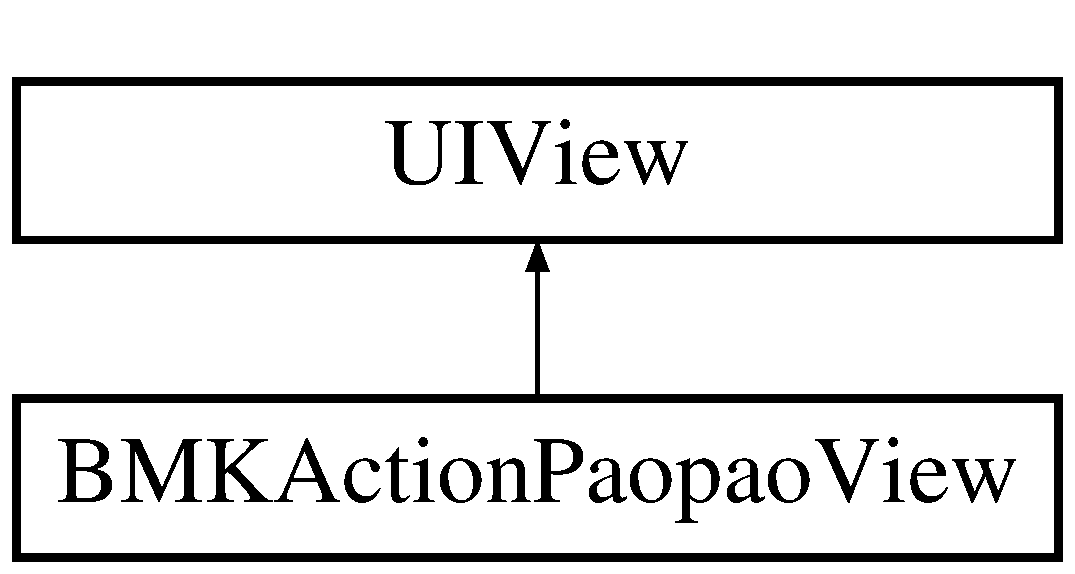
\includegraphics[height=2.000000cm]{interface_b_m_k_action_paopao_view}
\end{center}
\end{figure}
\subsection*{Instance Methods}
\begin{DoxyCompactItemize}
\item 
(id) -\/ \hyperlink{interface_b_m_k_action_paopao_view_ae6a2f4ea0ff6a408b963f6f1eb068ef5}{init\+With\+Custom\+View\+:}
\end{DoxyCompactItemize}


\subsection{详细描述}
该类用于定义一个\+Paopao\+View 

\subsection{Method Documentation}
\hypertarget{interface_b_m_k_action_paopao_view_ae6a2f4ea0ff6a408b963f6f1eb068ef5}{\index{B\+M\+K\+Action\+Paopao\+View@{B\+M\+K\+Action\+Paopao\+View}!init\+With\+Custom\+View\+:@{init\+With\+Custom\+View\+:}}
\index{init\+With\+Custom\+View\+:@{init\+With\+Custom\+View\+:}!B\+M\+K\+Action\+Paopao\+View@{B\+M\+K\+Action\+Paopao\+View}}
\subsubsection[{init\+With\+Custom\+View\+:}]{\setlength{\rightskip}{0pt plus 5cm}-\/ (id) init\+With\+Custom\+View\+: 
\begin{DoxyParamCaption}
\item[{(U\+I\+View $\ast$)}]{custom\+View}
\end{DoxyParamCaption}
}}\label{interface_b_m_k_action_paopao_view_ae6a2f4ea0ff6a408b963f6f1eb068ef5}
初始化并返回一个\+B\+M\+K\+Action\+Paopao\+View 
\begin{DoxyParams}{参数}
{\em custom\+View} & 自定义\+View,custom\+View=nil时返回默认的\+Paopao\+View \\
\hline
\end{DoxyParams}
\begin{DoxyReturn}{返回}
初始化成功则返回\+B\+M\+K\+Action\+Paopao\+View,否则返回nil 
\end{DoxyReturn}


该类的文档由以下文件生成\+:\begin{DoxyCompactItemize}
\item 
output/map\+\_\+search\+\_\+cloud\+\_\+loc\+\_\+util/inc/B\+M\+K\+Action\+Paopao\+View.\+h\end{DoxyCompactItemize}

\hypertarget{interface_b_m_k_address_component}{\section{B\+M\+K\+Address\+Component类 参考}
\label{interface_b_m_k_address_component}\index{B\+M\+K\+Address\+Component@{B\+M\+K\+Address\+Component}}
}


此类表示地址结果的层次化信息  




{\ttfamily \#import $<$B\+M\+K\+Geocode\+Type.\+h$>$}

类 B\+M\+K\+Address\+Component 继承关系图\+:\begin{figure}[H]
\begin{center}
\leavevmode
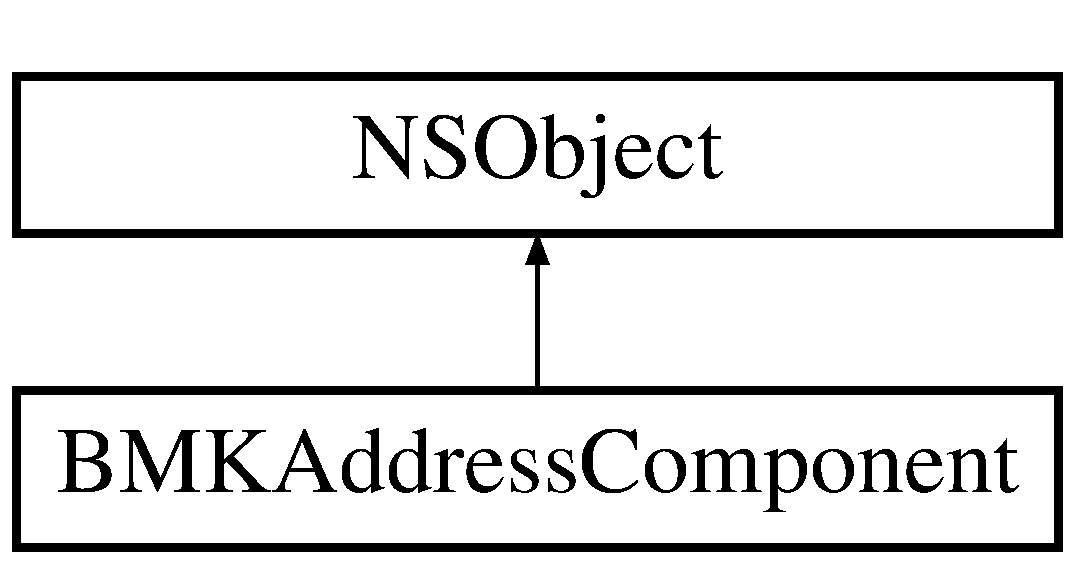
\includegraphics[height=2.000000cm]{interface_b_m_k_address_component}
\end{center}
\end{figure}
\subsection*{Protected 属性}
\begin{DoxyCompactItemize}
\item 
\hypertarget{interface_b_m_k_address_component_aa0266bba479e431954882b7ab5cbfa07}{N\+S\+String $\ast$ {\bfseries \+\_\+street\+Number}}\label{interface_b_m_k_address_component_aa0266bba479e431954882b7ab5cbfa07}

\item 
\hypertarget{interface_b_m_k_address_component_a8eb365c63cc3c5993b597658fc398181}{N\+S\+String $\ast$ {\bfseries \+\_\+street\+Name}}\label{interface_b_m_k_address_component_a8eb365c63cc3c5993b597658fc398181}

\item 
\hypertarget{interface_b_m_k_address_component_af95961f735ab9789f2be5e11a3ff6875}{N\+S\+String $\ast$ {\bfseries \+\_\+district}}\label{interface_b_m_k_address_component_af95961f735ab9789f2be5e11a3ff6875}

\item 
\hypertarget{interface_b_m_k_address_component_aedb7357a02424464616394fb9b051c56}{N\+S\+String $\ast$ {\bfseries \+\_\+city}}\label{interface_b_m_k_address_component_aedb7357a02424464616394fb9b051c56}

\item 
\hypertarget{interface_b_m_k_address_component_a233c3fae615c60ff44ce462fe7de7e30}{N\+S\+String $\ast$ {\bfseries \+\_\+province}}\label{interface_b_m_k_address_component_a233c3fae615c60ff44ce462fe7de7e30}

\end{DoxyCompactItemize}
\subsection*{属性}
\begin{DoxyCompactItemize}
\item 
\hypertarget{interface_b_m_k_address_component_a7a9e0a709b4969472aa1b17a042975c8}{N\+S\+String $\ast$ \hyperlink{interface_b_m_k_address_component_a7a9e0a709b4969472aa1b17a042975c8}{street\+Number}}\label{interface_b_m_k_address_component_a7a9e0a709b4969472aa1b17a042975c8}

\begin{DoxyCompactList}\small\item\em 街道号码 \end{DoxyCompactList}\item 
\hypertarget{interface_b_m_k_address_component_afef3697cbdab210a40b85a4d628aa6b8}{N\+S\+String $\ast$ \hyperlink{interface_b_m_k_address_component_afef3697cbdab210a40b85a4d628aa6b8}{street\+Name}}\label{interface_b_m_k_address_component_afef3697cbdab210a40b85a4d628aa6b8}

\begin{DoxyCompactList}\small\item\em 街道名称 \end{DoxyCompactList}\item 
\hypertarget{interface_b_m_k_address_component_a3bb4c8b38bef483378a4ed4e0ec33aaa}{N\+S\+String $\ast$ \hyperlink{interface_b_m_k_address_component_a3bb4c8b38bef483378a4ed4e0ec33aaa}{district}}\label{interface_b_m_k_address_component_a3bb4c8b38bef483378a4ed4e0ec33aaa}

\begin{DoxyCompactList}\small\item\em 区县名称 \end{DoxyCompactList}\item 
\hypertarget{interface_b_m_k_address_component_ad7a30c029e65d37d09d106ca5cb55d1b}{N\+S\+String $\ast$ \hyperlink{interface_b_m_k_address_component_ad7a30c029e65d37d09d106ca5cb55d1b}{city}}\label{interface_b_m_k_address_component_ad7a30c029e65d37d09d106ca5cb55d1b}

\begin{DoxyCompactList}\small\item\em 城市名称 \end{DoxyCompactList}\item 
\hypertarget{interface_b_m_k_address_component_a849d581c8eaa3447b9aaa1764f7ac85c}{N\+S\+String $\ast$ \hyperlink{interface_b_m_k_address_component_a849d581c8eaa3447b9aaa1764f7ac85c}{province}}\label{interface_b_m_k_address_component_a849d581c8eaa3447b9aaa1764f7ac85c}

\begin{DoxyCompactList}\small\item\em 省份名称 \end{DoxyCompactList}\end{DoxyCompactItemize}


\subsection{详细描述}
此类表示地址结果的层次化信息 

该类的文档由以下文件生成\+:\begin{DoxyCompactItemize}
\item 
output/map\+\_\+search\+\_\+cloud\+\_\+loc\+\_\+util/inc/B\+M\+K\+Geocode\+Type.\+h\end{DoxyCompactItemize}

\hypertarget{protocol_b_m_k_annotation-p}{\section{$<$B\+M\+K\+Annotation$>$协议 参考}
\label{protocol_b_m_k_annotation-p}\index{$<$\+B\+M\+K\+Annotation$>$@{$<$\+B\+M\+K\+Annotation$>$}}
}


该类为标注点的protocol,提供了标注类的基本信息函数  




{\ttfamily \#import $<$B\+M\+K\+Annotation.\+h$>$}

类 $<$B\+M\+K\+Annotation$>$ 继承关系图\+:\begin{figure}[H]
\begin{center}
\leavevmode
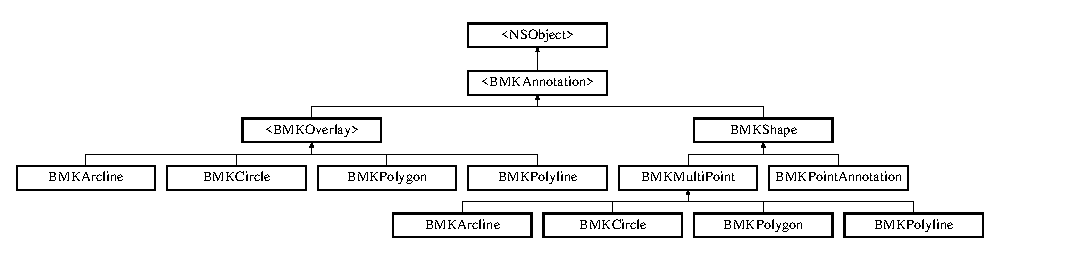
\includegraphics[height=2.962963cm]{protocol_b_m_k_annotation-p}
\end{center}
\end{figure}
\subsection*{Instance Methods}
\begin{DoxyCompactItemize}
\item 
(N\+S\+String $\ast$) -\/ \hyperlink{protocol_b_m_k_annotation-p_a249e1b880f8ded8541a0fe59ef4abb12}{title}
\item 
(N\+S\+String $\ast$) -\/ \hyperlink{protocol_b_m_k_annotation-p_a62aea71f4631251330e8a6fc3d3bdf11}{subtitle}
\item 
(void) -\/ \hyperlink{protocol_b_m_k_annotation-p_a86db1788af78d273e1e155d3aa3d978f}{set\+Coordinate\+:}
\end{DoxyCompactItemize}
\subsection*{属性}
\begin{DoxyCompactItemize}
\item 
\hypertarget{protocol_b_m_k_annotation-p_ab7ed7fd80fc518acf82cf0048490f9be}{C\+L\+Location\+Coordinate2\+D \hyperlink{protocol_b_m_k_annotation-p_ab7ed7fd80fc518acf82cf0048490f9be}{coordinate}}\label{protocol_b_m_k_annotation-p_ab7ed7fd80fc518acf82cf0048490f9be}

\begin{DoxyCompactList}\small\item\em 标注view中心坐标. \end{DoxyCompactList}\end{DoxyCompactItemize}


\subsection{详细描述}
该类为标注点的protocol,提供了标注类的基本信息函数 

\subsection{Method Documentation}
\hypertarget{protocol_b_m_k_annotation-p_a86db1788af78d273e1e155d3aa3d978f}{\index{B\+M\+K\+Annotation-\/p@{B\+M\+K\+Annotation-\/p}!set\+Coordinate\+:@{set\+Coordinate\+:}}
\index{set\+Coordinate\+:@{set\+Coordinate\+:}!B\+M\+K\+Annotation-\/p@{B\+M\+K\+Annotation-\/p}}
\subsubsection[{set\+Coordinate\+:}]{\setlength{\rightskip}{0pt plus 5cm}-\/ (void) set\+Coordinate\+: 
\begin{DoxyParamCaption}
\item[{(C\+L\+Location\+Coordinate2\+D)}]{new\+Coordinate}
\end{DoxyParamCaption}
\hspace{0.3cm}{\ttfamily [optional]}}}\label{protocol_b_m_k_annotation-p_a86db1788af78d273e1e155d3aa3d978f}
设置标注的坐标,在拖拽时会被调用. 
\begin{DoxyParams}{参数}
{\em new\+Coordinate} & 新的坐标值 \\
\hline
\end{DoxyParams}
\hypertarget{protocol_b_m_k_annotation-p_a62aea71f4631251330e8a6fc3d3bdf11}{\index{B\+M\+K\+Annotation-\/p@{B\+M\+K\+Annotation-\/p}!subtitle@{subtitle}}
\index{subtitle@{subtitle}!B\+M\+K\+Annotation-\/p@{B\+M\+K\+Annotation-\/p}}
\subsubsection[{subtitle}]{\setlength{\rightskip}{0pt plus 5cm}-\/ (N\+S\+String $\ast$) subtitle 
\begin{DoxyParamCaption}
{}
\end{DoxyParamCaption}
\hspace{0.3cm}{\ttfamily [optional]}}}\label{protocol_b_m_k_annotation-p_a62aea71f4631251330e8a6fc3d3bdf11}
获取annotation副标题 \begin{DoxyReturn}{返回}
返回annotation的副标题信息 
\end{DoxyReturn}
\hypertarget{protocol_b_m_k_annotation-p_a249e1b880f8ded8541a0fe59ef4abb12}{\index{B\+M\+K\+Annotation-\/p@{B\+M\+K\+Annotation-\/p}!title@{title}}
\index{title@{title}!B\+M\+K\+Annotation-\/p@{B\+M\+K\+Annotation-\/p}}
\subsubsection[{title}]{\setlength{\rightskip}{0pt plus 5cm}-\/ (N\+S\+String $\ast$) title 
\begin{DoxyParamCaption}
{}
\end{DoxyParamCaption}
\hspace{0.3cm}{\ttfamily [optional]}}}\label{protocol_b_m_k_annotation-p_a249e1b880f8ded8541a0fe59ef4abb12}
获取annotation标题 \begin{DoxyReturn}{返回}
返回annotation的标题信息 
\end{DoxyReturn}


该协议的文档由以下文件生成\+:\begin{DoxyCompactItemize}
\item 
output/map\+\_\+search\+\_\+cloud\+\_\+loc\+\_\+util/inc/B\+M\+K\+Annotation.\+h\end{DoxyCompactItemize}

\hypertarget{interface_b_m_k_annotation_view}{\section{B\+M\+K\+Annotation\+View类 参考}
\label{interface_b_m_k_annotation_view}\index{B\+M\+K\+Annotation\+View@{B\+M\+K\+Annotation\+View}}
}


标注view  




{\ttfamily \#import $<$B\+M\+K\+Annotation\+View.\+h$>$}

类 B\+M\+K\+Annotation\+View 继承关系图\+:\begin{figure}[H]
\begin{center}
\leavevmode
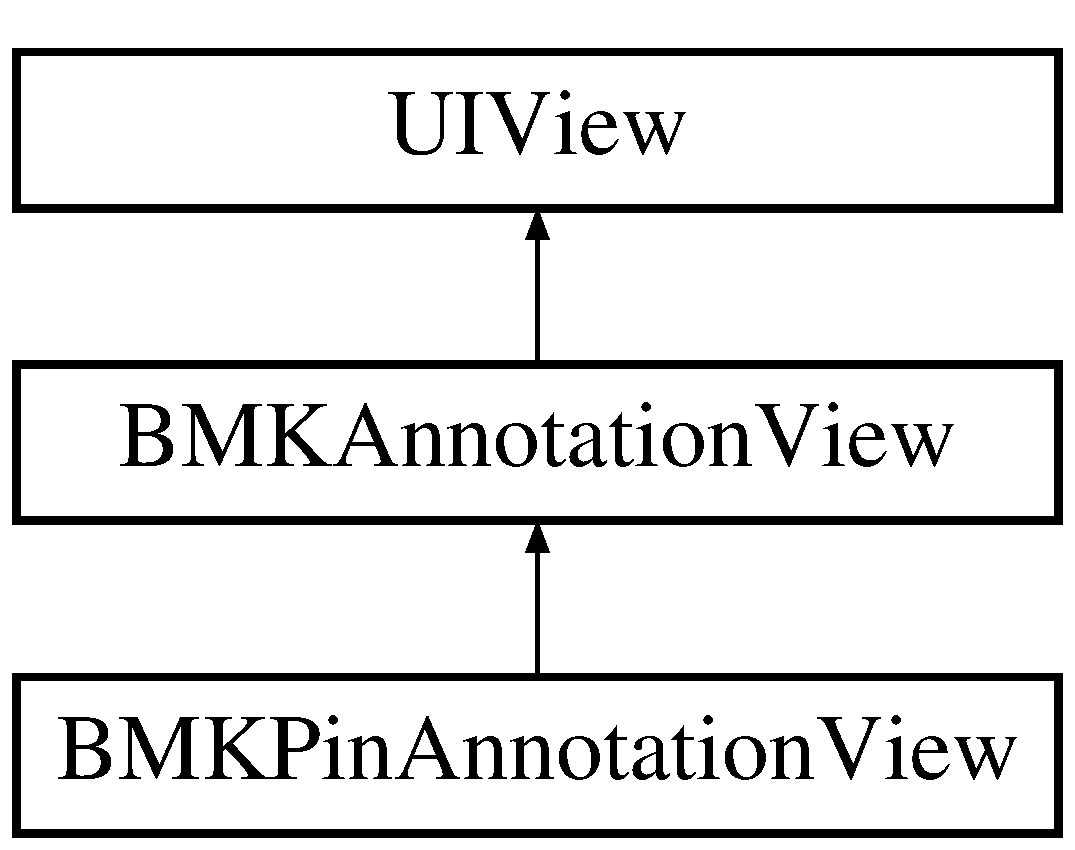
\includegraphics[height=3.000000cm]{interface_b_m_k_annotation_view}
\end{center}
\end{figure}
\subsection*{Instance Methods}
\begin{DoxyCompactItemize}
\item 
(id) -\/ \hyperlink{interface_b_m_k_annotation_view_ae2b46541ec52b7d8ee0857a9ec369f5f}{init\+With\+Annotation\+:reuse\+Identifier\+:}
\item 
(void) -\/ \hyperlink{interface_b_m_k_annotation_view_ae74849e624ac0cfaa7695b7cc97ddf23}{prepare\+For\+Reuse}
\item 
(void) -\/ \hyperlink{interface_b_m_k_annotation_view_abc0e70812fb7b3bccdbb574ddb578c21}{set\+Selected\+:animated\+:}
\item 
\hypertarget{interface_b_m_k_annotation_view_a54d15e7cc4e89d89d2233ec7fc408ad9}{(B\+O\+O\+L draggable) -\/ \hyperlink{interface_b_m_k_annotation_view_a54d15e7cc4e89d89d2233ec7fc408ad9}{\+\_\+\+\_\+\+O\+S\+X\+\_\+\+A\+V\+A\+I\+L\+A\+B\+L\+E\+\_\+\+S\+T\+A\+R\+T\+I\+N\+G}}\label{interface_b_m_k_annotation_view_a54d15e7cc4e89d89d2233ec7fc408ad9}

\begin{DoxyCompactList}\small\item\em 当设为\+Y\+E\+S并实现了set\+Coordinate\+:方法时,支持将view在地图上拖动, ios 3.\+2以后支持 \end{DoxyCompactList}\item 
\hypertarget{interface_b_m_k_annotation_view_a623e818d48c983176a6553104b21a34c}{(B\+M\+K\+Annotation\+View\+Drag\+State \\*
drag\+State) -\/ \hyperlink{interface_b_m_k_annotation_view_a623e818d48c983176a6553104b21a34c}{\+\_\+\+\_\+\+O\+S\+X\+\_\+\+A\+V\+A\+I\+L\+A\+B\+L\+E\+\_\+\+S\+T\+A\+R\+T\+I\+N\+G}}\label{interface_b_m_k_annotation_view_a623e818d48c983176a6553104b21a34c}

\begin{DoxyCompactList}\small\item\em 当前view的拖动状态, ios 3.\+2以后支持 \end{DoxyCompactList}\end{DoxyCompactItemize}
\subsection*{属性}
\begin{DoxyCompactItemize}
\item 
\hypertarget{interface_b_m_k_annotation_view_aba3efdbef49c0301af03ce0d47348358}{N\+S\+String $\ast$ \hyperlink{interface_b_m_k_annotation_view_aba3efdbef49c0301af03ce0d47348358}{reuse\+Identifier}}\label{interface_b_m_k_annotation_view_aba3efdbef49c0301af03ce0d47348358}

\begin{DoxyCompactList}\small\item\em 复用标志 \end{DoxyCompactList}\item 
\hypertarget{interface_b_m_k_annotation_view_af351c55cfa4b90f2e5090f0503ff699c}{\hyperlink{interface_b_m_k_action_paopao_view}{B\+M\+K\+Action\+Paopao\+View} $\ast$ \hyperlink{interface_b_m_k_annotation_view_af351c55cfa4b90f2e5090f0503ff699c}{paopao\+View}}\label{interface_b_m_k_annotation_view_af351c55cfa4b90f2e5090f0503ff699c}

\begin{DoxyCompactList}\small\item\em paopao\+View \end{DoxyCompactList}\item 
\hypertarget{interface_b_m_k_annotation_view_a466f040671f2235667a4034aba879bb5}{id$<$ \hyperlink{protocol_b_m_k_annotation-p}{B\+M\+K\+Annotation} $>$ \hyperlink{interface_b_m_k_annotation_view_a466f040671f2235667a4034aba879bb5}{annotation}}\label{interface_b_m_k_annotation_view_a466f040671f2235667a4034aba879bb5}

\begin{DoxyCompactList}\small\item\em 关联的annotation \end{DoxyCompactList}\item 
\hypertarget{interface_b_m_k_annotation_view_a3186f78dcb098002e39fd226cbc1c9b6}{U\+I\+Image $\ast$ \hyperlink{interface_b_m_k_annotation_view_a3186f78dcb098002e39fd226cbc1c9b6}{image}}\label{interface_b_m_k_annotation_view_a3186f78dcb098002e39fd226cbc1c9b6}

\begin{DoxyCompactList}\small\item\em annotation view显示的图像 \end{DoxyCompactList}\item 
\hypertarget{interface_b_m_k_annotation_view_a12a4f32e8adc7732c80d772eb403cd61}{C\+G\+Point \hyperlink{interface_b_m_k_annotation_view_a12a4f32e8adc7732c80d772eb403cd61}{center\+Offset}}\label{interface_b_m_k_annotation_view_a12a4f32e8adc7732c80d772eb403cd61}

\begin{DoxyCompactList}\small\item\em 默认情况下, annotation view的中心位于annotation的坐标位置,可以设置center\+Offset改变view的位置,正的偏移使view朝右下方移动,负的朝左上方,单位是像素 \end{DoxyCompactList}\item 
\hypertarget{interface_b_m_k_annotation_view_aacdcb492cbbc469803ba50def87f44e5}{C\+G\+Point \hyperlink{interface_b_m_k_annotation_view_aacdcb492cbbc469803ba50def87f44e5}{callout\+Offset}}\label{interface_b_m_k_annotation_view_aacdcb492cbbc469803ba50def87f44e5}

\begin{DoxyCompactList}\small\item\em 默认情况下, 弹出的气泡位于view正中上方,可以设置callout\+Offset改变view的位置,正的偏移使view朝右下方移动,负的朝左上方,单位是像素 \end{DoxyCompactList}\item 
\hypertarget{interface_b_m_k_annotation_view_a18cef771d9b9feeb74a4bc4dd7fba526}{B\+O\+O\+L \hyperlink{interface_b_m_k_annotation_view_a18cef771d9b9feeb74a4bc4dd7fba526}{enabled3\+D}}\label{interface_b_m_k_annotation_view_a18cef771d9b9feeb74a4bc4dd7fba526}

\begin{DoxyCompactList}\small\item\em 默认情况下,标注没有3\+D效果,可以设置enabled3\+D改变使用3\+D效果,使得标注在地图旋转和俯视时跟随旋转、俯视 \end{DoxyCompactList}\item 
\hypertarget{interface_b_m_k_annotation_view_ad768885a75146458b4efd168885478fe}{B\+O\+O\+L \hyperlink{interface_b_m_k_annotation_view_ad768885a75146458b4efd168885478fe}{enabled}}\label{interface_b_m_k_annotation_view_ad768885a75146458b4efd168885478fe}

\begin{DoxyCompactList}\small\item\em 默认为\+Y\+E\+S,当为\+N\+O时view忽略触摸事件 \end{DoxyCompactList}\item 
\hypertarget{interface_b_m_k_annotation_view_a09799664ef861651bd7996f0fbab6483}{B\+O\+O\+L \hyperlink{interface_b_m_k_annotation_view_a09799664ef861651bd7996f0fbab6483}{selected}}\label{interface_b_m_k_annotation_view_a09799664ef861651bd7996f0fbab6483}

\begin{DoxyCompactList}\small\item\em 默认为\+N\+O,当view被点中时被设为\+Y\+E\+S,用户不要直接设置这个属性. \end{DoxyCompactList}\item 
\hypertarget{interface_b_m_k_annotation_view_adef94e946f5b152c59be1cdb5eccfb74}{B\+O\+O\+L \hyperlink{interface_b_m_k_annotation_view_adef94e946f5b152c59be1cdb5eccfb74}{can\+Show\+Callout}}\label{interface_b_m_k_annotation_view_adef94e946f5b152c59be1cdb5eccfb74}

\begin{DoxyCompactList}\small\item\em 当为\+Y\+E\+S时,view被选中时会弹出气泡,annotation必须实现了title这个方法 \end{DoxyCompactList}\item 
\hypertarget{interface_b_m_k_annotation_view_ae182c0fb7dc1898c4941a123def7f926}{U\+I\+View $\ast$ \hyperlink{interface_b_m_k_annotation_view_ae182c0fb7dc1898c4941a123def7f926}{left\+Callout\+Accessory\+View}}\label{interface_b_m_k_annotation_view_ae182c0fb7dc1898c4941a123def7f926}

\begin{DoxyCompactList}\small\item\em 显示在气泡左侧的view \end{DoxyCompactList}\item 
\hypertarget{interface_b_m_k_annotation_view_a65793288845c27e23233373b3e6b6216}{U\+I\+View $\ast$ \hyperlink{interface_b_m_k_annotation_view_a65793288845c27e23233373b3e6b6216}{right\+Callout\+Accessory\+View}}\label{interface_b_m_k_annotation_view_a65793288845c27e23233373b3e6b6216}

\begin{DoxyCompactList}\small\item\em 显示在气泡右侧的view \end{DoxyCompactList}\end{DoxyCompactItemize}


\subsection{详细描述}
标注view 

\subsection{Method Documentation}
\hypertarget{interface_b_m_k_annotation_view_ae2b46541ec52b7d8ee0857a9ec369f5f}{\index{B\+M\+K\+Annotation\+View@{B\+M\+K\+Annotation\+View}!init\+With\+Annotation\+:reuse\+Identifier\+:@{init\+With\+Annotation\+:reuse\+Identifier\+:}}
\index{init\+With\+Annotation\+:reuse\+Identifier\+:@{init\+With\+Annotation\+:reuse\+Identifier\+:}!B\+M\+K\+Annotation\+View@{B\+M\+K\+Annotation\+View}}
\subsubsection[{init\+With\+Annotation\+:reuse\+Identifier\+:}]{\setlength{\rightskip}{0pt plus 5cm}-\/ (id) init\+With\+Annotation\+: 
\begin{DoxyParamCaption}
\item[{(id$<$ {\bf B\+M\+K\+Annotation} $>$)}]{annotation}
\item[{reuseIdentifier:(N\+S\+String $\ast$)}]{reuse\+Identifier}
\end{DoxyParamCaption}
}}\label{interface_b_m_k_annotation_view_ae2b46541ec52b7d8ee0857a9ec369f5f}
初始化并返回一个annotation view 
\begin{DoxyParams}{参数}
{\em annotation} & 关联的annotation对象 \\
\hline
{\em reuse\+Identifier} & 如果要重用view,传入一个字符串,否则设为nil,建议重用view \\
\hline
\end{DoxyParams}
\begin{DoxyReturn}{返回}
初始化成功则返回annotation view,否则返回nil 
\end{DoxyReturn}
\hypertarget{interface_b_m_k_annotation_view_ae74849e624ac0cfaa7695b7cc97ddf23}{\index{B\+M\+K\+Annotation\+View@{B\+M\+K\+Annotation\+View}!prepare\+For\+Reuse@{prepare\+For\+Reuse}}
\index{prepare\+For\+Reuse@{prepare\+For\+Reuse}!B\+M\+K\+Annotation\+View@{B\+M\+K\+Annotation\+View}}
\subsubsection[{prepare\+For\+Reuse}]{\setlength{\rightskip}{0pt plus 5cm}-\/ (void) prepare\+For\+Reuse 
\begin{DoxyParamCaption}
{}
\end{DoxyParamCaption}
}}\label{interface_b_m_k_annotation_view_ae74849e624ac0cfaa7695b7cc97ddf23}
当view从reuse队列里取出时被调用 默认不做任何事 \hypertarget{interface_b_m_k_annotation_view_abc0e70812fb7b3bccdbb574ddb578c21}{\index{B\+M\+K\+Annotation\+View@{B\+M\+K\+Annotation\+View}!set\+Selected\+:animated\+:@{set\+Selected\+:animated\+:}}
\index{set\+Selected\+:animated\+:@{set\+Selected\+:animated\+:}!B\+M\+K\+Annotation\+View@{B\+M\+K\+Annotation\+View}}
\subsubsection[{set\+Selected\+:animated\+:}]{\setlength{\rightskip}{0pt plus 5cm}-\/ (void) set\+Selected\+: 
\begin{DoxyParamCaption}
\item[{(B\+O\+O\+L)}]{selected}
\item[{animated:(B\+O\+O\+L)}]{animated}
\end{DoxyParamCaption}
}}\label{interface_b_m_k_annotation_view_abc0e70812fb7b3bccdbb574ddb578c21}
设定view的选中状态 该方法被\+B\+M\+K\+Map\+View调用 
\begin{DoxyParams}{参数}
{\em selected} & 如果view需要显示为选中状态,该值为\+Y\+E\+S \\
\hline
{\em animated} & 如果需要动画效果,该值为\+Y\+E\+S,暂不支持 \\
\hline
\end{DoxyParams}


该类的文档由以下文件生成\+:\begin{DoxyCompactItemize}
\item 
output/map\+\_\+search\+\_\+cloud\+\_\+loc\+\_\+util/inc/B\+M\+K\+Annotation\+View.\+h\end{DoxyCompactItemize}

\hypertarget{interface_b_m_k_arcline}{\section{B\+M\+K\+Arcline类 参考}
\label{interface_b_m_k_arcline}\index{B\+M\+K\+Arcline@{B\+M\+K\+Arcline}}
}


此类用于定义一段圆弧  




{\ttfamily \#import $<$B\+M\+K\+Arcline.\+h$>$}

类 B\+M\+K\+Arcline 继承关系图\+:\begin{figure}[H]
\begin{center}
\leavevmode
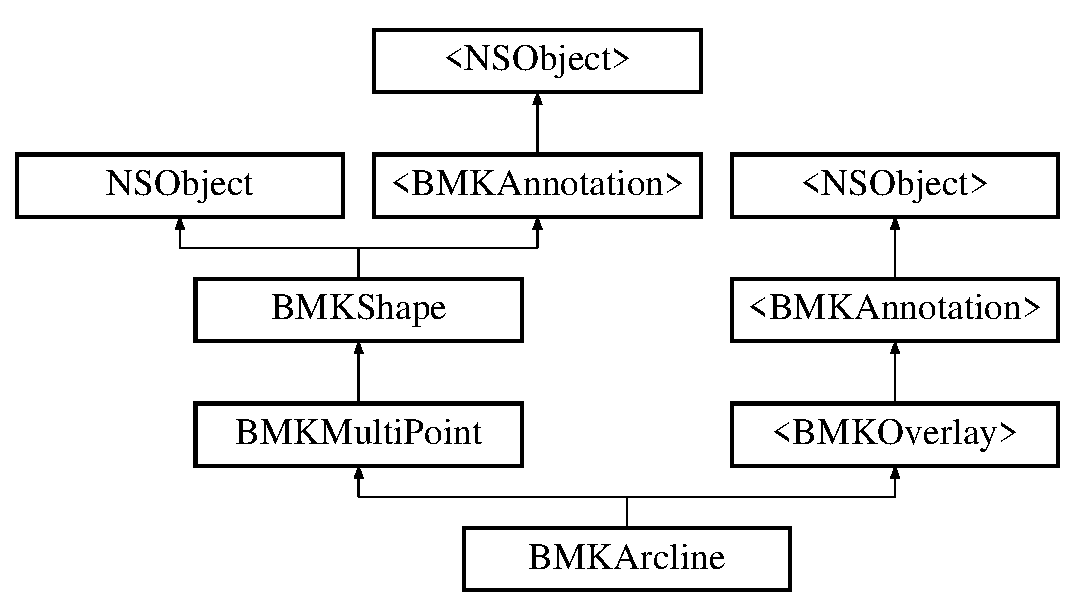
\includegraphics[height=5.000000cm]{interface_b_m_k_arcline}
\end{center}
\end{figure}
\subsection*{Class Methods}
\begin{DoxyCompactItemize}
\item 
(\hyperlink{interface_b_m_k_arcline}{B\+M\+K\+Arcline} $\ast$) + \hyperlink{interface_b_m_k_arcline_ad439d6682d48b51c0b04e84772a38a79}{arcline\+With\+Points\+:}
\item 
(\hyperlink{interface_b_m_k_arcline}{B\+M\+K\+Arcline} $\ast$) + \hyperlink{interface_b_m_k_arcline_a34a5daa9fc480861aa52e2ef5b0ccb3a}{arcline\+With\+Coordinates\+:}
\end{DoxyCompactItemize}
\subsection*{Protected 属性}
\begin{DoxyCompactItemize}
\item 
\hypertarget{interface_b_m_k_arcline_abbb8f0dba8c81ab8bcd8cc8e587d51cf}{\hyperlink{struct_b_m_k_map_rect}{B\+M\+K\+Map\+Rect} {\bfseries \+\_\+bounding\+Map\+Rect}}\label{interface_b_m_k_arcline_abbb8f0dba8c81ab8bcd8cc8e587d51cf}

\item 
\hypertarget{interface_b_m_k_arcline_ae74be329c0bfedce99b890f70d3b871e}{bool {\bfseries is\+You\+Arc}}\label{interface_b_m_k_arcline_ae74be329c0bfedce99b890f70d3b871e}

\end{DoxyCompactItemize}
\subsection*{额外继承的成员函数}


\subsection{详细描述}
此类用于定义一段圆弧 

\subsection{Method Documentation}
\hypertarget{interface_b_m_k_arcline_a34a5daa9fc480861aa52e2ef5b0ccb3a}{\index{B\+M\+K\+Arcline@{B\+M\+K\+Arcline}!arcline\+With\+Coordinates\+:@{arcline\+With\+Coordinates\+:}}
\index{arcline\+With\+Coordinates\+:@{arcline\+With\+Coordinates\+:}!B\+M\+K\+Arcline@{B\+M\+K\+Arcline}}
\subsubsection[{arcline\+With\+Coordinates\+:}]{\setlength{\rightskip}{0pt plus 5cm}+ ({\bf B\+M\+K\+Arcline} $\ast$) arcline\+With\+Coordinates\+: 
\begin{DoxyParamCaption}
\item[{(C\+L\+Location\+Coordinate2\+D $\ast$)}]{coords}
\end{DoxyParamCaption}
}}\label{interface_b_m_k_arcline_a34a5daa9fc480861aa52e2ef5b0ccb3a}
根据指定经纬度生成一段圆弧 
\begin{DoxyParams}{参数}
{\em coords} & 指定的经纬度坐标点数组 \\
\hline
\end{DoxyParams}
\begin{DoxyReturn}{返回}
新生成的圆弧对象 
\end{DoxyReturn}
\hypertarget{interface_b_m_k_arcline_ad439d6682d48b51c0b04e84772a38a79}{\index{B\+M\+K\+Arcline@{B\+M\+K\+Arcline}!arcline\+With\+Points\+:@{arcline\+With\+Points\+:}}
\index{arcline\+With\+Points\+:@{arcline\+With\+Points\+:}!B\+M\+K\+Arcline@{B\+M\+K\+Arcline}}
\subsubsection[{arcline\+With\+Points\+:}]{\setlength{\rightskip}{0pt plus 5cm}+ ({\bf B\+M\+K\+Arcline} $\ast$) arcline\+With\+Points\+: 
\begin{DoxyParamCaption}
\item[{({\bf B\+M\+K\+Map\+Point} $\ast$)}]{points}
\end{DoxyParamCaption}
}}\label{interface_b_m_k_arcline_ad439d6682d48b51c0b04e84772a38a79}
根据指定坐标点生成一段圆弧 
\begin{DoxyParams}{参数}
{\em points} & 指定的直角坐标点数组 \\
\hline
\end{DoxyParams}
\begin{DoxyReturn}{返回}
新生成的圆弧对象 
\end{DoxyReturn}


该类的文档由以下文件生成\+:\begin{DoxyCompactItemize}
\item 
output/map\+\_\+search\+\_\+cloud\+\_\+loc\+\_\+util/inc/B\+M\+K\+Arcline.\+h\end{DoxyCompactItemize}

\hypertarget{interface_b_m_k_arcline_view}{\section{B\+M\+K\+Arcline\+View类 参考}
\label{interface_b_m_k_arcline_view}\index{B\+M\+K\+Arcline\+View@{B\+M\+K\+Arcline\+View}}
}


此类用于定义一个圆弧\+View  




{\ttfamily \#import $<$B\+M\+K\+Arcline\+View.\+h$>$}

类 B\+M\+K\+Arcline\+View 继承关系图\+:\begin{figure}[H]
\begin{center}
\leavevmode
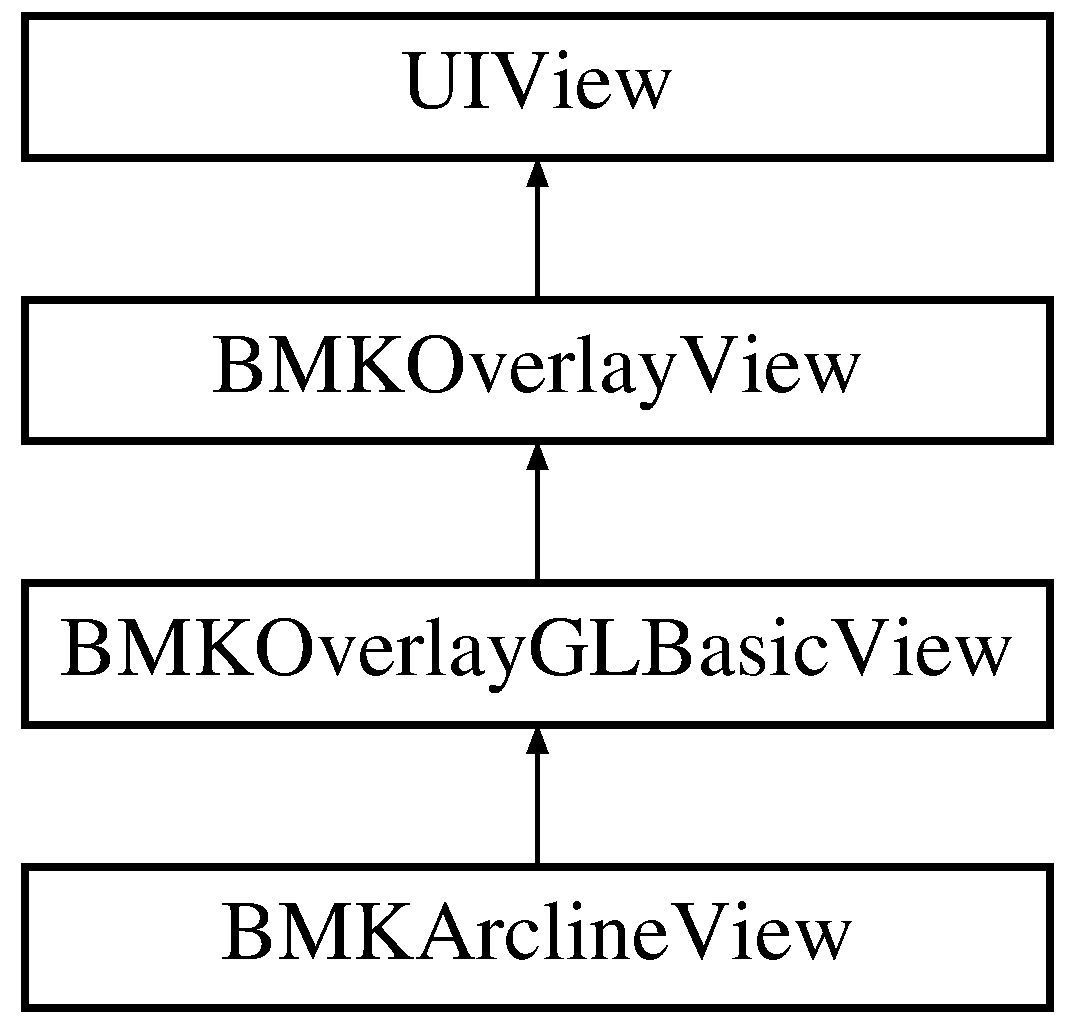
\includegraphics[height=4.000000cm]{interface_b_m_k_arcline_view}
\end{center}
\end{figure}
\subsection*{Instance Methods}
\begin{DoxyCompactItemize}
\item 
(id) -\/ \hyperlink{interface_b_m_k_arcline_view_ab5f05370f8d16895a04be3fb4168210a}{init\+With\+Arcline\+:}
\end{DoxyCompactItemize}
\subsection*{属性}
\begin{DoxyCompactItemize}
\item 
\hypertarget{interface_b_m_k_arcline_view_a824cf05f5bd4ff3790e78095ee72e6c2}{\hyperlink{interface_b_m_k_arcline}{B\+M\+K\+Arcline} $\ast$ \hyperlink{interface_b_m_k_arcline_view_a824cf05f5bd4ff3790e78095ee72e6c2}{arcline}}\label{interface_b_m_k_arcline_view_a824cf05f5bd4ff3790e78095ee72e6c2}

\begin{DoxyCompactList}\small\item\em 该\+View对应的圆弧数据对象 \end{DoxyCompactList}\end{DoxyCompactItemize}
\subsection*{额外继承的成员函数}


\subsection{详细描述}
此类用于定义一个圆弧\+View 

\subsection{Method Documentation}
\hypertarget{interface_b_m_k_arcline_view_ab5f05370f8d16895a04be3fb4168210a}{\index{B\+M\+K\+Arcline\+View@{B\+M\+K\+Arcline\+View}!init\+With\+Arcline\+:@{init\+With\+Arcline\+:}}
\index{init\+With\+Arcline\+:@{init\+With\+Arcline\+:}!B\+M\+K\+Arcline\+View@{B\+M\+K\+Arcline\+View}}
\subsubsection[{init\+With\+Arcline\+:}]{\setlength{\rightskip}{0pt plus 5cm}-\/ (id) init\+With\+Arcline\+: 
\begin{DoxyParamCaption}
\item[{({\bf B\+M\+K\+Arcline} $\ast$)}]{arcline}
\end{DoxyParamCaption}
}}\label{interface_b_m_k_arcline_view_ab5f05370f8d16895a04be3fb4168210a}
根据指定的弧线生成一个圆弧\+View 
\begin{DoxyParams}{参数}
{\em arcline} & 指定的弧线数据对象 \\
\hline
\end{DoxyParams}
\begin{DoxyReturn}{返回}
新生成的弧线\+View 
\end{DoxyReturn}


该类的文档由以下文件生成\+:\begin{DoxyCompactItemize}
\item 
output/map\+\_\+search\+\_\+cloud\+\_\+loc\+\_\+util/inc/B\+M\+K\+Arcline\+View.\+h\end{DoxyCompactItemize}

\hypertarget{interface_b_m_k_base_cloud_search_info}{\section{B\+M\+K\+Base\+Cloud\+Search\+Info类 参考}
\label{interface_b_m_k_base_cloud_search_info}\index{B\+M\+K\+Base\+Cloud\+Search\+Info@{B\+M\+K\+Base\+Cloud\+Search\+Info}}
}


云检索基础信息类,所有类型云检索的基类  




{\ttfamily \#import $<$B\+M\+K\+Cloud\+Search\+Info.\+h$>$}

类 B\+M\+K\+Base\+Cloud\+Search\+Info 继承关系图\+:\begin{figure}[H]
\begin{center}
\leavevmode
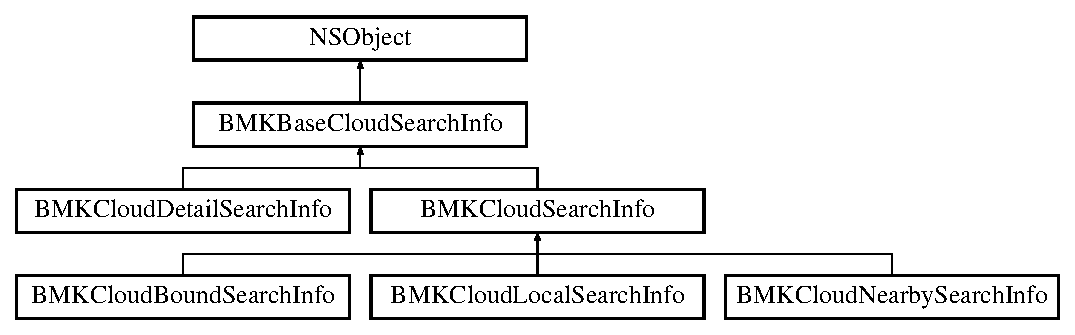
\includegraphics[height=4.000000cm]{interface_b_m_k_base_cloud_search_info}
\end{center}
\end{figure}
\subsection*{Protected 属性}
\begin{DoxyCompactItemize}
\item 
\hypertarget{interface_b_m_k_base_cloud_search_info_a7e0ee4faf41da0365d2f427b677f621a}{N\+S\+String $\ast$ {\bfseries \+\_\+ak}}\label{interface_b_m_k_base_cloud_search_info_a7e0ee4faf41da0365d2f427b677f621a}

\item 
\hypertarget{interface_b_m_k_base_cloud_search_info_a2c8bc1521f7025190278e3f29647c652}{N\+S\+String $\ast$ {\bfseries \+\_\+sn}}\label{interface_b_m_k_base_cloud_search_info_a2c8bc1521f7025190278e3f29647c652}

\item 
\hypertarget{interface_b_m_k_base_cloud_search_info_a3d23b81d16c3054a5b73c2f017b435c3}{int {\bfseries \+\_\+geo\+Table\+Id}}\label{interface_b_m_k_base_cloud_search_info_a3d23b81d16c3054a5b73c2f017b435c3}

\end{DoxyCompactItemize}
\subsection*{属性}
\begin{DoxyCompactItemize}
\item 
\hypertarget{interface_b_m_k_base_cloud_search_info_a3ac025d61069505d4ff685e4c77b78a4}{N\+S\+String $\ast$ \hyperlink{interface_b_m_k_base_cloud_search_info_a3ac025d61069505d4ff685e4c77b78a4}{ak}}\label{interface_b_m_k_base_cloud_search_info_a3ac025d61069505d4ff685e4c77b78a4}

\begin{DoxyCompactList}\small\item\em access\+\_\+key(必须),最大长度50 \end{DoxyCompactList}\item 
\hypertarget{interface_b_m_k_base_cloud_search_info_a0dcbea8108d264a217566025d43aff12}{N\+S\+String $\ast$ \hyperlink{interface_b_m_k_base_cloud_search_info_a0dcbea8108d264a217566025d43aff12}{sn}}\label{interface_b_m_k_base_cloud_search_info_a0dcbea8108d264a217566025d43aff12}

\begin{DoxyCompactList}\small\item\em 用户的权限签名,(可选),最大长度50 \end{DoxyCompactList}\item 
\hypertarget{interface_b_m_k_base_cloud_search_info_acb6f48270abf3f46a0412bcd658d099c}{int \hyperlink{interface_b_m_k_base_cloud_search_info_acb6f48270abf3f46a0412bcd658d099c}{geo\+Table\+Id}}\label{interface_b_m_k_base_cloud_search_info_acb6f48270abf3f46a0412bcd658d099c}

\begin{DoxyCompactList}\small\item\em geo table 表主键(必须) \end{DoxyCompactList}\end{DoxyCompactItemize}


\subsection{详细描述}
云检索基础信息类,所有类型云检索的基类 

该类的文档由以下文件生成\+:\begin{DoxyCompactItemize}
\item 
output/map\+\_\+search\+\_\+cloud\+\_\+loc\+\_\+util/inc/B\+M\+K\+Cloud\+Search\+Info.\+h\end{DoxyCompactItemize}

\hypertarget{interface_b_m_k_base_poi_search_option}{\section{B\+M\+K\+Base\+Poi\+Search\+Option类 参考}
\label{interface_b_m_k_base_poi_search_option}\index{B\+M\+K\+Base\+Poi\+Search\+Option@{B\+M\+K\+Base\+Poi\+Search\+Option}}
}


检索基础信息类,所有类型\+Poi检索的基类  




{\ttfamily \#import $<$B\+M\+K\+Poi\+Search\+Option.\+h$>$}

类 B\+M\+K\+Base\+Poi\+Search\+Option 继承关系图\+:\begin{figure}[H]
\begin{center}
\leavevmode
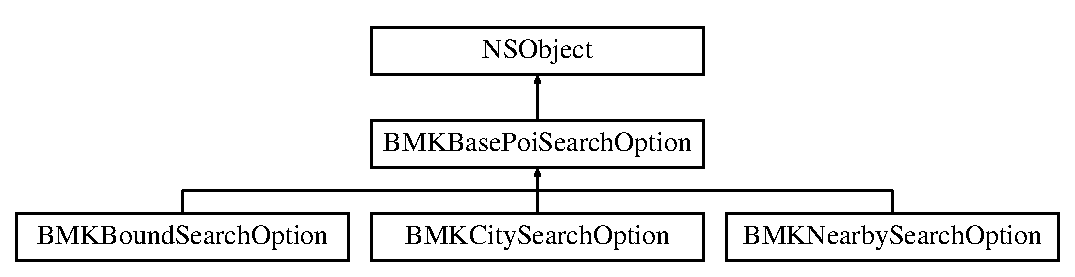
\includegraphics[height=3.000000cm]{interface_b_m_k_base_poi_search_option}
\end{center}
\end{figure}
\subsection*{Protected 属性}
\begin{DoxyCompactItemize}
\item 
\hypertarget{interface_b_m_k_base_poi_search_option_aec623956bb8cfc11c5d5959c6cf698da}{N\+S\+String $\ast$ {\bfseries \+\_\+keyword}}\label{interface_b_m_k_base_poi_search_option_aec623956bb8cfc11c5d5959c6cf698da}

\item 
\hypertarget{interface_b_m_k_base_poi_search_option_a9d3de22e269b9f69806e8f0b077d039f}{int {\bfseries \+\_\+page\+Index}}\label{interface_b_m_k_base_poi_search_option_a9d3de22e269b9f69806e8f0b077d039f}

\item 
\hypertarget{interface_b_m_k_base_poi_search_option_aa2e8a12a6101e57ec5e384f1cef92429}{int {\bfseries \+\_\+page\+Capacity}}\label{interface_b_m_k_base_poi_search_option_aa2e8a12a6101e57ec5e384f1cef92429}

\end{DoxyCompactItemize}
\subsection*{属性}
\begin{DoxyCompactItemize}
\item 
\hypertarget{interface_b_m_k_base_poi_search_option_af74b52da74e6d70c2904774938d4358a}{N\+S\+String $\ast$ \hyperlink{interface_b_m_k_base_poi_search_option_af74b52da74e6d70c2904774938d4358a}{keyword}}\label{interface_b_m_k_base_poi_search_option_af74b52da74e6d70c2904774938d4358a}

\begin{DoxyCompactList}\small\item\em 搜索关键字 \end{DoxyCompactList}\item 
\hypertarget{interface_b_m_k_base_poi_search_option_a23b7f5ccb9cdb0c77dc80e57039be011}{int \hyperlink{interface_b_m_k_base_poi_search_option_a23b7f5ccb9cdb0c77dc80e57039be011}{page\+Index}}\label{interface_b_m_k_base_poi_search_option_a23b7f5ccb9cdb0c77dc80e57039be011}

\begin{DoxyCompactList}\small\item\em 分页索引,可选,默认为0 \end{DoxyCompactList}\item 
\hypertarget{interface_b_m_k_base_poi_search_option_a6c4467b4e1f98bebf75d59f95b6fc85d}{int \hyperlink{interface_b_m_k_base_poi_search_option_a6c4467b4e1f98bebf75d59f95b6fc85d}{page\+Capacity}}\label{interface_b_m_k_base_poi_search_option_a6c4467b4e1f98bebf75d59f95b6fc85d}

\begin{DoxyCompactList}\small\item\em 分页数量,可选,默认为10,最多为50 \end{DoxyCompactList}\end{DoxyCompactItemize}


\subsection{详细描述}
检索基础信息类,所有类型\+Poi检索的基类 

该类的文档由以下文件生成\+:\begin{DoxyCompactItemize}
\item 
output/map\+\_\+search\+\_\+cloud\+\_\+loc\+\_\+util/inc/B\+M\+K\+Poi\+Search\+Option.\+h\end{DoxyCompactItemize}

\hypertarget{interface_b_m_k_base_route_plan_option}{\section{B\+M\+K\+Base\+Route\+Plan\+Option类 参考}
\label{interface_b_m_k_base_route_plan_option}\index{B\+M\+K\+Base\+Route\+Plan\+Option@{B\+M\+K\+Base\+Route\+Plan\+Option}}
}


路线查询基础信息类  




{\ttfamily \#import $<$B\+M\+K\+Route\+Search\+Option.\+h$>$}

类 B\+M\+K\+Base\+Route\+Plan\+Option 继承关系图\+:\begin{figure}[H]
\begin{center}
\leavevmode
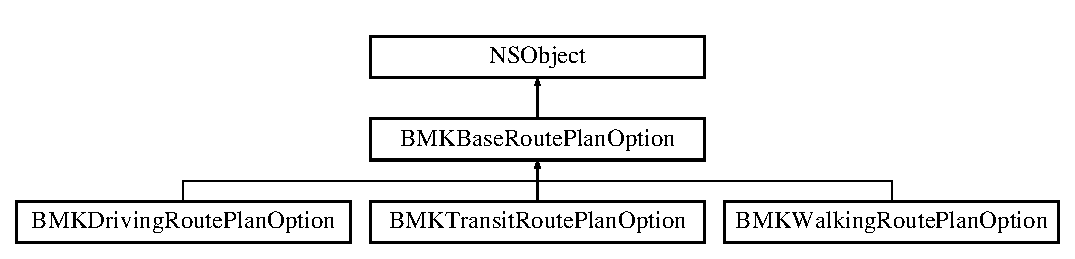
\includegraphics[height=3.000000cm]{interface_b_m_k_base_route_plan_option}
\end{center}
\end{figure}
\subsection*{Protected 属性}
\begin{DoxyCompactItemize}
\item 
\hypertarget{interface_b_m_k_base_route_plan_option_a1a668d22cbdfdf6f4b619522a5c24482}{\hyperlink{interface_b_m_k_plan_node}{B\+M\+K\+Plan\+Node} $\ast$ {\bfseries \+\_\+from}}\label{interface_b_m_k_base_route_plan_option_a1a668d22cbdfdf6f4b619522a5c24482}

\item 
\hypertarget{interface_b_m_k_base_route_plan_option_a57edc8a986cecead42fef9e55949157c}{\hyperlink{interface_b_m_k_plan_node}{B\+M\+K\+Plan\+Node} $\ast$ {\bfseries \+\_\+to}}\label{interface_b_m_k_base_route_plan_option_a57edc8a986cecead42fef9e55949157c}

\end{DoxyCompactItemize}
\subsection*{属性}
\begin{DoxyCompactItemize}
\item 
\hypertarget{interface_b_m_k_base_route_plan_option_afb4bc6a8468e1bf3dbb24c86abf06827}{\hyperlink{interface_b_m_k_plan_node}{B\+M\+K\+Plan\+Node} $\ast$ \hyperlink{interface_b_m_k_base_route_plan_option_afb4bc6a8468e1bf3dbb24c86abf06827}{from}}\label{interface_b_m_k_base_route_plan_option_afb4bc6a8468e1bf3dbb24c86abf06827}

\begin{DoxyCompactList}\small\item\em 检索的起点,可通过关键字、坐标两种方式指定 \end{DoxyCompactList}\item 
\hypertarget{interface_b_m_k_base_route_plan_option_a6a01852ca226bdc1f580bb4a10745c62}{\hyperlink{interface_b_m_k_plan_node}{B\+M\+K\+Plan\+Node} $\ast$ \hyperlink{interface_b_m_k_base_route_plan_option_a6a01852ca226bdc1f580bb4a10745c62}{to}}\label{interface_b_m_k_base_route_plan_option_a6a01852ca226bdc1f580bb4a10745c62}

\begin{DoxyCompactList}\small\item\em 检索的终点,可通过关键字、坐标两种方式指定 \end{DoxyCompactList}\end{DoxyCompactItemize}


\subsection{详细描述}
路线查询基础信息类 

该类的文档由以下文件生成\+:\begin{DoxyCompactItemize}
\item 
output/map\+\_\+search\+\_\+cloud\+\_\+loc\+\_\+util/inc/B\+M\+K\+Route\+Search\+Option.\+h\end{DoxyCompactItemize}

\hypertarget{interface_b_m_k_bound_search_option}{\section{B\+M\+K\+Bound\+Search\+Option类 参考}
\label{interface_b_m_k_bound_search_option}\index{B\+M\+K\+Bound\+Search\+Option@{B\+M\+K\+Bound\+Search\+Option}}
}


矩形云检索参数信息类  




{\ttfamily \#import $<$B\+M\+K\+Poi\+Search\+Option.\+h$>$}

类 B\+M\+K\+Bound\+Search\+Option 继承关系图\+:\begin{figure}[H]
\begin{center}
\leavevmode
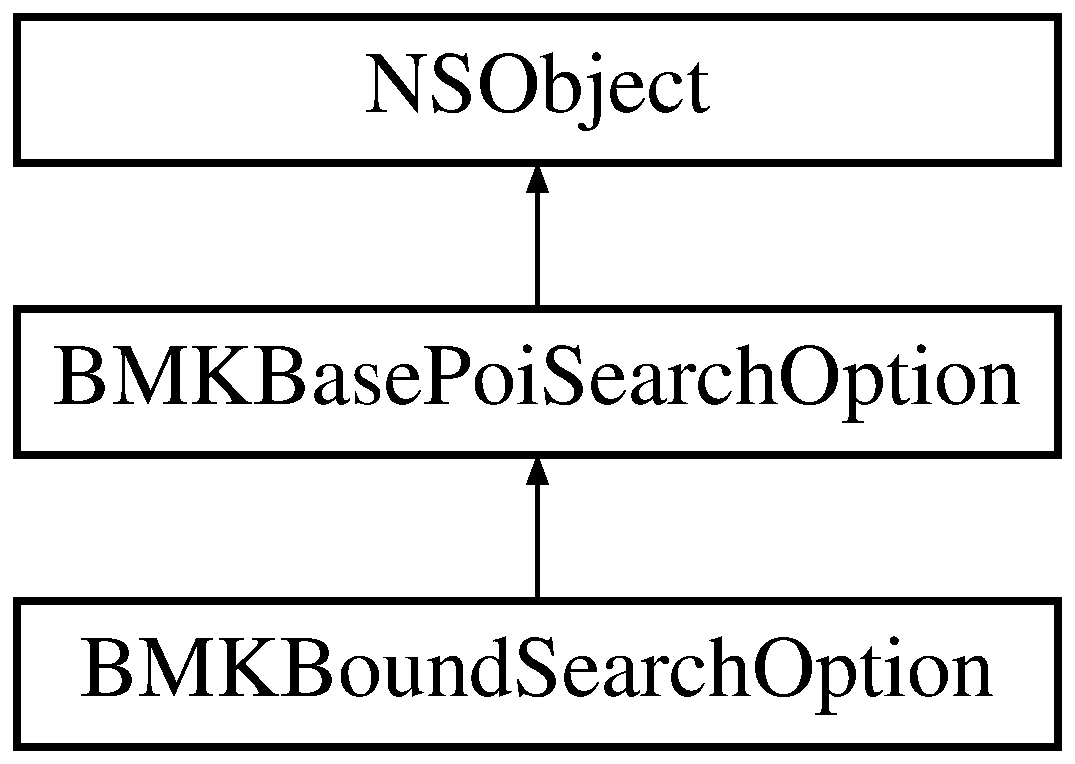
\includegraphics[height=3.000000cm]{interface_b_m_k_bound_search_option}
\end{center}
\end{figure}
\subsection*{Protected 属性}
\begin{DoxyCompactItemize}
\item 
\hypertarget{interface_b_m_k_bound_search_option_a439e395186d7cb9f72bb2cea6c112a26}{C\+L\+Location\+Coordinate2\+D {\bfseries \+\_\+left\+Bottom}}\label{interface_b_m_k_bound_search_option_a439e395186d7cb9f72bb2cea6c112a26}

\item 
\hypertarget{interface_b_m_k_bound_search_option_a4bd165343e4ea38ceabb6da210c90793}{C\+L\+Location\+Coordinate2\+D {\bfseries \+\_\+right\+Top}}\label{interface_b_m_k_bound_search_option_a4bd165343e4ea38ceabb6da210c90793}

\end{DoxyCompactItemize}
\subsection*{属性}
\begin{DoxyCompactItemize}
\item 
\hypertarget{interface_b_m_k_bound_search_option_ad68044c4ded82d49551ea014f20e5b67}{C\+L\+Location\+Coordinate2\+D \hyperlink{interface_b_m_k_bound_search_option_ad68044c4ded82d49551ea014f20e5b67}{left\+Bottom}}\label{interface_b_m_k_bound_search_option_ad68044c4ded82d49551ea014f20e5b67}

\begin{DoxyCompactList}\small\item\em 矩形区域,左下角和右上角的经纬度坐标点。 \end{DoxyCompactList}\item 
\hypertarget{interface_b_m_k_bound_search_option_a6864fdcb6ad4d284a17a31d76a4e54f8}{C\+L\+Location\+Coordinate2\+D {\bfseries right\+Top}}\label{interface_b_m_k_bound_search_option_a6864fdcb6ad4d284a17a31d76a4e54f8}

\end{DoxyCompactItemize}


\subsection{详细描述}
矩形云检索参数信息类 

该类的文档由以下文件生成\+:\begin{DoxyCompactItemize}
\item 
output/map\+\_\+search\+\_\+cloud\+\_\+loc\+\_\+util/inc/B\+M\+K\+Poi\+Search\+Option.\+h\end{DoxyCompactItemize}

\hypertarget{interface_b_m_k_bus_line_result}{\section{B\+M\+K\+Bus\+Line\+Result类 参考}
\label{interface_b_m_k_bus_line_result}\index{B\+M\+K\+Bus\+Line\+Result@{B\+M\+K\+Bus\+Line\+Result}}
}


此类表示公共交通信息查询结果  




{\ttfamily \#import $<$B\+M\+K\+Route\+Search\+Type.\+h$>$}

类 B\+M\+K\+Bus\+Line\+Result 继承关系图\+:\begin{figure}[H]
\begin{center}
\leavevmode
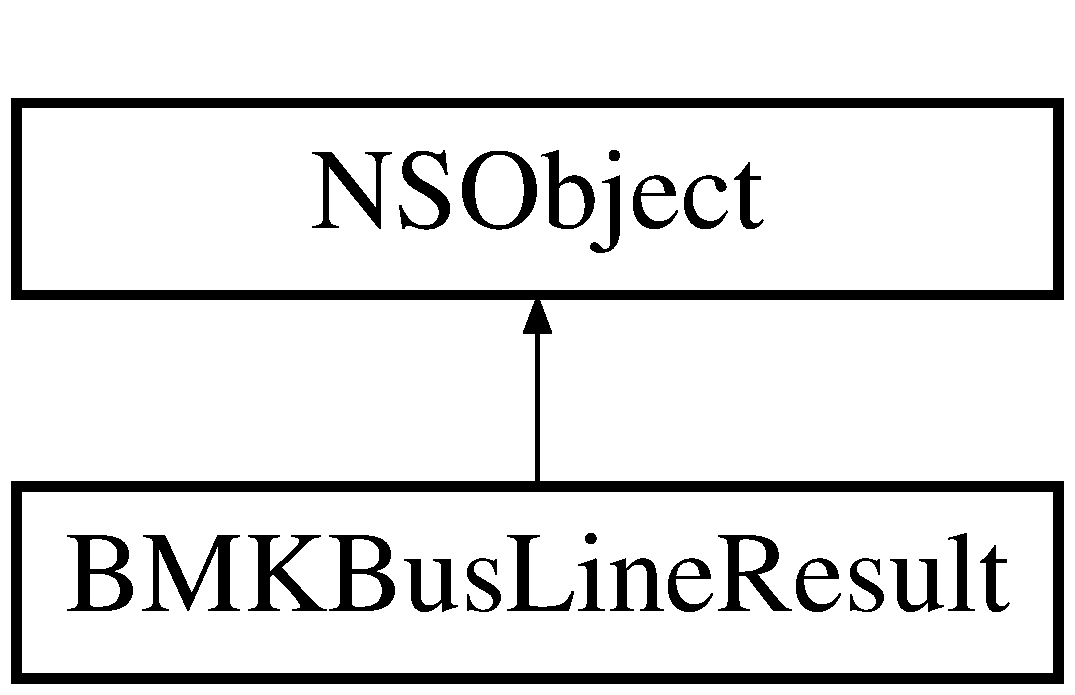
\includegraphics[height=2.000000cm]{interface_b_m_k_bus_line_result}
\end{center}
\end{figure}
\subsection*{Protected 属性}
\begin{DoxyCompactItemize}
\item 
\hypertarget{interface_b_m_k_bus_line_result_aee7114770e2a79b6e7251f02620d9db8}{N\+S\+String $\ast$ {\bfseries \+\_\+bus\+Company}}\label{interface_b_m_k_bus_line_result_aee7114770e2a79b6e7251f02620d9db8}

\item 
\hypertarget{interface_b_m_k_bus_line_result_a4e808af429044d025496bde44a7ebe9a}{N\+S\+String $\ast$ {\bfseries \+\_\+bus\+Line\+Name}}\label{interface_b_m_k_bus_line_result_a4e808af429044d025496bde44a7ebe9a}

\item 
\hypertarget{interface_b_m_k_bus_line_result_a1f62568a2f5223570aa368ef69ee30d1}{N\+S\+String $\ast$ {\bfseries \+\_\+uid}}\label{interface_b_m_k_bus_line_result_a1f62568a2f5223570aa368ef69ee30d1}

\item 
\hypertarget{interface_b_m_k_bus_line_result_a3fa16167a58b75ecfcabdcae7a540f62}{N\+S\+String $\ast$ {\bfseries \+\_\+start\+Time}}\label{interface_b_m_k_bus_line_result_a3fa16167a58b75ecfcabdcae7a540f62}

\item 
\hypertarget{interface_b_m_k_bus_line_result_acdac46e5cde2e8e71fc5a66912cca622}{N\+S\+String $\ast$ {\bfseries \+\_\+end\+Time}}\label{interface_b_m_k_bus_line_result_acdac46e5cde2e8e71fc5a66912cca622}

\item 
\hypertarget{interface_b_m_k_bus_line_result_a5c1f994e7352d047f6dbc8c1d5c39776}{int {\bfseries \+\_\+is\+Mon\+Ticket}}\label{interface_b_m_k_bus_line_result_a5c1f994e7352d047f6dbc8c1d5c39776}

\item 
\hypertarget{interface_b_m_k_bus_line_result_a4884541cd5344ae4f5a32de53bcc51b9}{N\+S\+Array $\ast$ {\bfseries \+\_\+bus\+Stations}}\label{interface_b_m_k_bus_line_result_a4884541cd5344ae4f5a32de53bcc51b9}

\item 
\hypertarget{interface_b_m_k_bus_line_result_ad0c810738565c208509cb7e7d52859e9}{N\+S\+Array $\ast$ {\bfseries \+\_\+bus\+Steps}}\label{interface_b_m_k_bus_line_result_ad0c810738565c208509cb7e7d52859e9}

\end{DoxyCompactItemize}
\subsection*{属性}
\begin{DoxyCompactItemize}
\item 
\hypertarget{interface_b_m_k_bus_line_result_a7ecd49d7ffa31f0d5b0a3f38c678f2bd}{N\+S\+String $\ast$ \hyperlink{interface_b_m_k_bus_line_result_a7ecd49d7ffa31f0d5b0a3f38c678f2bd}{bus\+Company}}\label{interface_b_m_k_bus_line_result_a7ecd49d7ffa31f0d5b0a3f38c678f2bd}

\begin{DoxyCompactList}\small\item\em 公交公司名称 \end{DoxyCompactList}\item 
\hypertarget{interface_b_m_k_bus_line_result_a5bbf221cefe58aa67edf770eaaf23a81}{N\+S\+String $\ast$ \hyperlink{interface_b_m_k_bus_line_result_a5bbf221cefe58aa67edf770eaaf23a81}{bus\+Line\+Name}}\label{interface_b_m_k_bus_line_result_a5bbf221cefe58aa67edf770eaaf23a81}

\begin{DoxyCompactList}\small\item\em 公交线路名称 \end{DoxyCompactList}\item 
\hypertarget{interface_b_m_k_bus_line_result_aaa4925efede5021b4c08e6c011a005de}{N\+S\+String $\ast$ \hyperlink{interface_b_m_k_bus_line_result_aaa4925efede5021b4c08e6c011a005de}{uid}}\label{interface_b_m_k_bus_line_result_aaa4925efede5021b4c08e6c011a005de}

\begin{DoxyCompactList}\small\item\em 公交线路uid \end{DoxyCompactList}\item 
\hypertarget{interface_b_m_k_bus_line_result_a884e91eeb4adda0d053fd98b84afa0ba}{N\+S\+String $\ast$ \hyperlink{interface_b_m_k_bus_line_result_a884e91eeb4adda0d053fd98b84afa0ba}{start\+Time}}\label{interface_b_m_k_bus_line_result_a884e91eeb4adda0d053fd98b84afa0ba}

\begin{DoxyCompactList}\small\item\em 公交路线首班车时间 \end{DoxyCompactList}\item 
\hypertarget{interface_b_m_k_bus_line_result_aec007f4464a050b671052ef32abad8f8}{N\+S\+String $\ast$ \hyperlink{interface_b_m_k_bus_line_result_aec007f4464a050b671052ef32abad8f8}{end\+Time}}\label{interface_b_m_k_bus_line_result_aec007f4464a050b671052ef32abad8f8}

\begin{DoxyCompactList}\small\item\em 公交路线末班车时间 \end{DoxyCompactList}\item 
\hypertarget{interface_b_m_k_bus_line_result_a2c311dc1e3378a192ffacdb2c3654ade}{int \hyperlink{interface_b_m_k_bus_line_result_a2c311dc1e3378a192ffacdb2c3654ade}{is\+Mon\+Ticket}}\label{interface_b_m_k_bus_line_result_a2c311dc1e3378a192ffacdb2c3654ade}

\begin{DoxyCompactList}\small\item\em 公交是线是否有月票 \end{DoxyCompactList}\item 
\hypertarget{interface_b_m_k_bus_line_result_a9fe3884161bea9c3955a65eebbb00d70}{N\+S\+Array $\ast$ \hyperlink{interface_b_m_k_bus_line_result_a9fe3884161bea9c3955a65eebbb00d70}{bus\+Stations}}\label{interface_b_m_k_bus_line_result_a9fe3884161bea9c3955a65eebbb00d70}

\begin{DoxyCompactList}\small\item\em 所有公交站点信息,成员类型为\+B\+M\+K\+Bus\+Station \end{DoxyCompactList}\item 
\hypertarget{interface_b_m_k_bus_line_result_acbb640c72f6b2649ee131c95fd826407}{N\+S\+Array $\ast$ \hyperlink{interface_b_m_k_bus_line_result_acbb640c72f6b2649ee131c95fd826407}{bus\+Steps}}\label{interface_b_m_k_bus_line_result_acbb640c72f6b2649ee131c95fd826407}

\begin{DoxyCompactList}\small\item\em 公交路线分段信息,成员类型为\+B\+M\+K\+Bus\+Step \end{DoxyCompactList}\end{DoxyCompactItemize}


\subsection{详细描述}
此类表示公共交通信息查询结果 

该类的文档由以下文件生成\+:\begin{DoxyCompactItemize}
\item 
output/map\+\_\+search\+\_\+cloud\+\_\+loc\+\_\+util/inc/B\+M\+K\+Route\+Search\+Type.\+h\end{DoxyCompactItemize}

\hypertarget{interface_b_m_k_bus_line_search}{\section{B\+M\+K\+Bus\+Line\+Search类 参考}
\label{interface_b_m_k_bus_line_search}\index{B\+M\+K\+Bus\+Line\+Search@{B\+M\+K\+Bus\+Line\+Search}}
}


busline搜索服务  




{\ttfamily \#import $<$B\+M\+K\+Bus\+Line\+Search.\+h$>$}

类 B\+M\+K\+Bus\+Line\+Search 继承关系图\+:\begin{figure}[H]
\begin{center}
\leavevmode
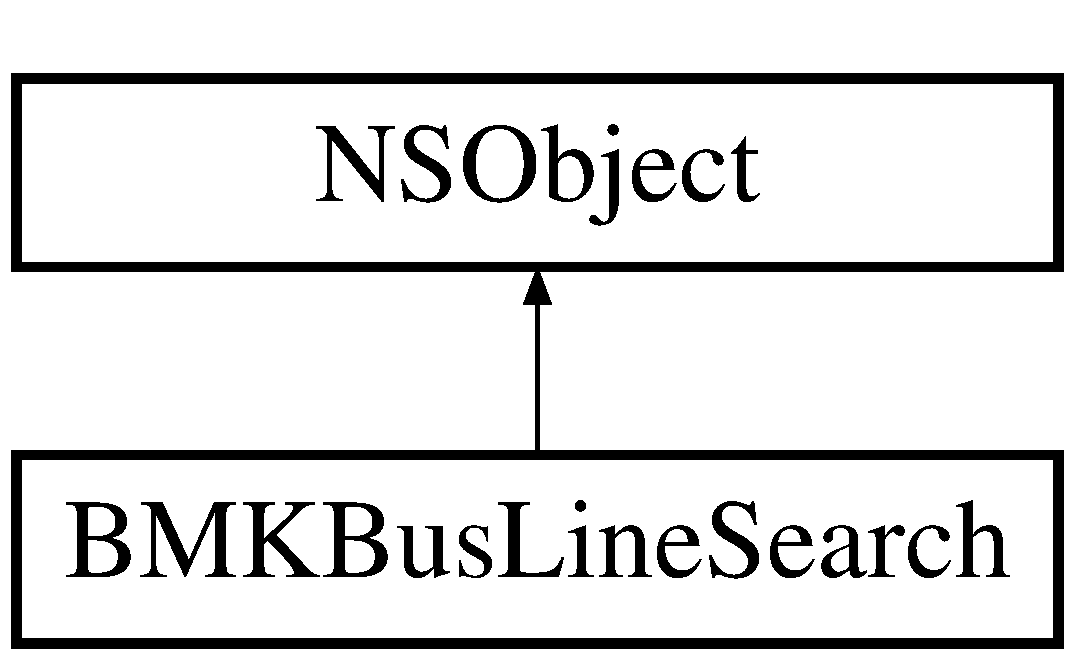
\includegraphics[height=2.000000cm]{interface_b_m_k_bus_line_search}
\end{center}
\end{figure}
\subsection*{Instance Methods}
\begin{DoxyCompactItemize}
\item 
(B\+O\+O\+L) -\/ \hyperlink{interface_b_m_k_bus_line_search_a652cac8a9fbaa46ddd7a0b09f5af8644}{bus\+Line\+Search\+:}
\end{DoxyCompactItemize}
\subsection*{属性}
\begin{DoxyCompactItemize}
\item 
\hypertarget{interface_b_m_k_bus_line_search_a87ccf434516c41498d6744f988e748a4}{id$<$ \hyperlink{protocol_b_m_k_bus_line_search_delegate-p}{B\+M\+K\+Bus\+Line\+Search\+Delegate} $>$ \hyperlink{interface_b_m_k_bus_line_search_a87ccf434516c41498d6744f988e748a4}{delegate}}\label{interface_b_m_k_bus_line_search_a87ccf434516c41498d6744f988e748a4}

\begin{DoxyCompactList}\small\item\em 检索模块的\+Delegate,此处记得不用的时候需要置nil,否则影响内存的释放 \end{DoxyCompactList}\end{DoxyCompactItemize}


\subsection{详细描述}
busline搜索服务 

\subsection{Method Documentation}
\hypertarget{interface_b_m_k_bus_line_search_a652cac8a9fbaa46ddd7a0b09f5af8644}{\index{B\+M\+K\+Bus\+Line\+Search@{B\+M\+K\+Bus\+Line\+Search}!bus\+Line\+Search\+:@{bus\+Line\+Search\+:}}
\index{bus\+Line\+Search\+:@{bus\+Line\+Search\+:}!B\+M\+K\+Bus\+Line\+Search@{B\+M\+K\+Bus\+Line\+Search}}
\subsubsection[{bus\+Line\+Search\+:}]{\setlength{\rightskip}{0pt plus 5cm}-\/ (B\+O\+O\+L) bus\+Line\+Search\+: 
\begin{DoxyParamCaption}
\item[{({\bf B\+M\+K\+Bus\+Line\+Search\+Option} $\ast$)}]{bus\+Line\+Search\+Option}
\end{DoxyParamCaption}
}}\label{interface_b_m_k_bus_line_search_a652cac8a9fbaa46ddd7a0b09f5af8644}
公交详情检索 异步函数,返回结果在\+B\+M\+K\+Bus\+Line\+Search\+Delegate的on\+Get\+Bus\+Detail\+Result通知 
\begin{DoxyParams}{参数}
{\em bus\+Line\+Search\+Option} & 公交线路检索信息类 \\
\hline
\end{DoxyParams}
\begin{DoxyReturn}{返回}
成功返回\+Y\+E\+S,否则返回\+N\+O 
\end{DoxyReturn}


该类的文档由以下文件生成\+:\begin{DoxyCompactItemize}
\item 
output/map\+\_\+search\+\_\+cloud\+\_\+loc\+\_\+util/inc/B\+M\+K\+Bus\+Line\+Search.\+h\end{DoxyCompactItemize}

\hypertarget{protocol_b_m_k_bus_line_search_delegate-p}{\section{$<$B\+M\+K\+Bus\+Line\+Search\+Delegate$>$协议 参考}
\label{protocol_b_m_k_bus_line_search_delegate-p}\index{$<$\+B\+M\+K\+Bus\+Line\+Search\+Delegate$>$@{$<$\+B\+M\+K\+Bus\+Line\+Search\+Delegate$>$}}
}


搜索delegate,用于获取搜索结果  




{\ttfamily \#import $<$B\+M\+K\+Bus\+Line\+Search.\+h$>$}

类 $<$B\+M\+K\+Bus\+Line\+Search\+Delegate$>$ 继承关系图\+:\begin{figure}[H]
\begin{center}
\leavevmode
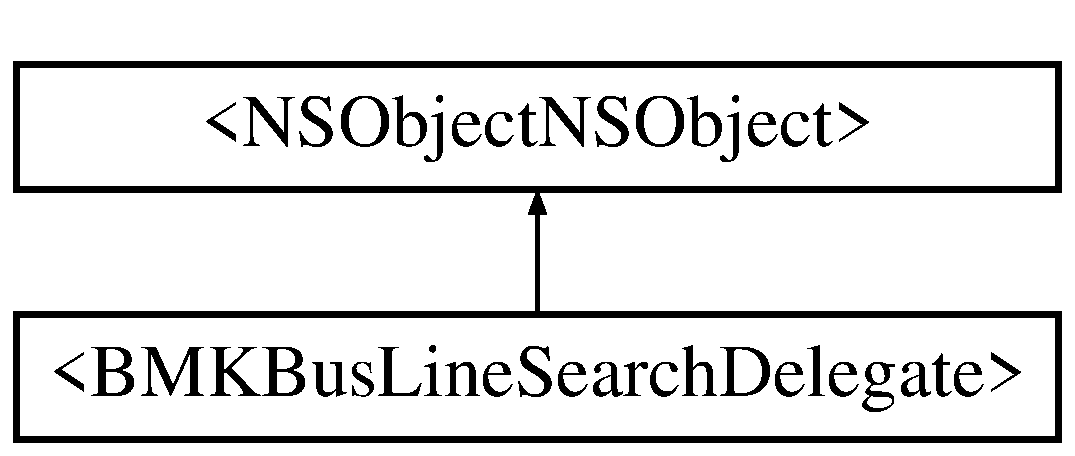
\includegraphics[height=2.000000cm]{protocol_b_m_k_bus_line_search_delegate-p}
\end{center}
\end{figure}
\subsection*{Instance Methods}
\begin{DoxyCompactItemize}
\item 
(void) -\/ \hyperlink{protocol_b_m_k_bus_line_search_delegate-p_ae1c5bce88d11150d38f8179368f39137}{on\+Get\+Bus\+Detail\+Result\+:result\+:error\+Code\+:}
\end{DoxyCompactItemize}


\subsection{详细描述}
搜索delegate,用于获取搜索结果 

\subsection{Method Documentation}
\hypertarget{protocol_b_m_k_bus_line_search_delegate-p_ae1c5bce88d11150d38f8179368f39137}{\index{B\+M\+K\+Bus\+Line\+Search\+Delegate-\/p@{B\+M\+K\+Bus\+Line\+Search\+Delegate-\/p}!on\+Get\+Bus\+Detail\+Result\+:result\+:error\+Code\+:@{on\+Get\+Bus\+Detail\+Result\+:result\+:error\+Code\+:}}
\index{on\+Get\+Bus\+Detail\+Result\+:result\+:error\+Code\+:@{on\+Get\+Bus\+Detail\+Result\+:result\+:error\+Code\+:}!B\+M\+K\+Bus\+Line\+Search\+Delegate-\/p@{B\+M\+K\+Bus\+Line\+Search\+Delegate-\/p}}
\subsubsection[{on\+Get\+Bus\+Detail\+Result\+:result\+:error\+Code\+:}]{\setlength{\rightskip}{0pt plus 5cm}-\/ (void) on\+Get\+Bus\+Detail\+Result\+: 
\begin{DoxyParamCaption}
\item[{({\bf B\+M\+K\+Bus\+Line\+Search} $\ast$)}]{searcher}
\item[{result:({\bf B\+M\+K\+Bus\+Line\+Result} $\ast$)}]{bus\+Line\+Result}
\item[{errorCode:(B\+M\+K\+Search\+Error\+Code)}]{error}
\end{DoxyParamCaption}
\hspace{0.3cm}{\ttfamily [optional]}}}\label{protocol_b_m_k_bus_line_search_delegate-p_ae1c5bce88d11150d38f8179368f39137}
返回busdetail搜索结果 
\begin{DoxyParams}{参数}
{\em searcher} & 搜索对象 \\
\hline
{\em bus\+Line\+Result} & 搜索结果 \\
\hline
{\em error} & 错误号,\\
\hline
\end{DoxyParams}
\begin{DoxySeeAlso}{参见}
B\+M\+K\+Search\+Error\+Code 
\end{DoxySeeAlso}


该协议的文档由以下文件生成\+:\begin{DoxyCompactItemize}
\item 
output/map\+\_\+search\+\_\+cloud\+\_\+loc\+\_\+util/inc/B\+M\+K\+Bus\+Line\+Search.\+h\end{DoxyCompactItemize}

\hypertarget{interface_b_m_k_bus_line_search_option}{\section{B\+M\+K\+Bus\+Line\+Search\+Option类 参考}
\label{interface_b_m_k_bus_line_search_option}\index{B\+M\+K\+Bus\+Line\+Search\+Option@{B\+M\+K\+Bus\+Line\+Search\+Option}}
}


公交线路检索信息类  




{\ttfamily \#import $<$B\+M\+K\+Bus\+Line\+Search\+Option.\+h$>$}

类 B\+M\+K\+Bus\+Line\+Search\+Option 继承关系图\+:\begin{figure}[H]
\begin{center}
\leavevmode
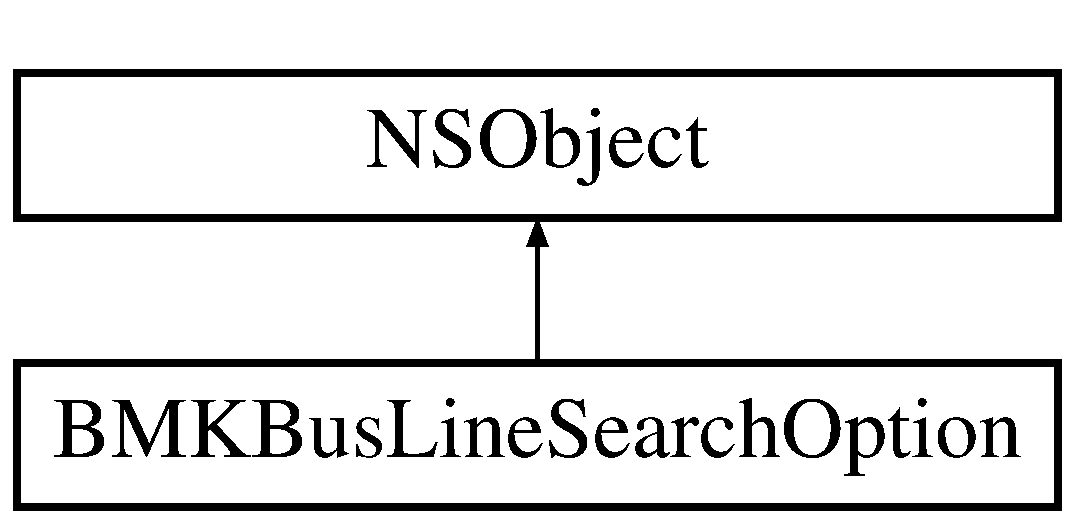
\includegraphics[height=2.000000cm]{interface_b_m_k_bus_line_search_option}
\end{center}
\end{figure}
\subsection*{Protected 属性}
\begin{DoxyCompactItemize}
\item 
\hypertarget{interface_b_m_k_bus_line_search_option_a7a4d92693254a3f0d2c1e79b3a5eb88b}{N\+S\+String $\ast$ {\bfseries \+\_\+city}}\label{interface_b_m_k_bus_line_search_option_a7a4d92693254a3f0d2c1e79b3a5eb88b}

\item 
\hypertarget{interface_b_m_k_bus_line_search_option_a382c85171a018c5487143fd560068c39}{N\+S\+String $\ast$ {\bfseries \+\_\+bus\+Line\+Uid}}\label{interface_b_m_k_bus_line_search_option_a382c85171a018c5487143fd560068c39}

\end{DoxyCompactItemize}
\subsection*{属性}
\begin{DoxyCompactItemize}
\item 
\hypertarget{interface_b_m_k_bus_line_search_option_ac8dc465234c79e3882cddbd3e16ff21a}{N\+S\+String $\ast$ \hyperlink{interface_b_m_k_bus_line_search_option_ac8dc465234c79e3882cddbd3e16ff21a}{city}}\label{interface_b_m_k_bus_line_search_option_ac8dc465234c79e3882cddbd3e16ff21a}

\begin{DoxyCompactList}\small\item\em 城市名 \end{DoxyCompactList}\item 
\hypertarget{interface_b_m_k_bus_line_search_option_ac514e5b1930f97cecca6821562877146}{N\+S\+String $\ast$ \hyperlink{interface_b_m_k_bus_line_search_option_ac514e5b1930f97cecca6821562877146}{bus\+Line\+Uid}}\label{interface_b_m_k_bus_line_search_option_ac514e5b1930f97cecca6821562877146}

\begin{DoxyCompactList}\small\item\em 公交线路的uid \end{DoxyCompactList}\end{DoxyCompactItemize}


\subsection{详细描述}
公交线路检索信息类 

该类的文档由以下文件生成\+:\begin{DoxyCompactItemize}
\item 
output/map\+\_\+search\+\_\+cloud\+\_\+loc\+\_\+util/inc/B\+M\+K\+Bus\+Line\+Search\+Option.\+h\end{DoxyCompactItemize}

\hypertarget{interface_b_m_k_bus_station}{\section{B\+M\+K\+Bus\+Station类 参考}
\label{interface_b_m_k_bus_station}\index{B\+M\+K\+Bus\+Station@{B\+M\+K\+Bus\+Station}}
}


此类表示公交站点信息  




{\ttfamily \#import $<$B\+M\+K\+Route\+Search\+Type.\+h$>$}

类 B\+M\+K\+Bus\+Station 继承关系图\+:\begin{figure}[H]
\begin{center}
\leavevmode
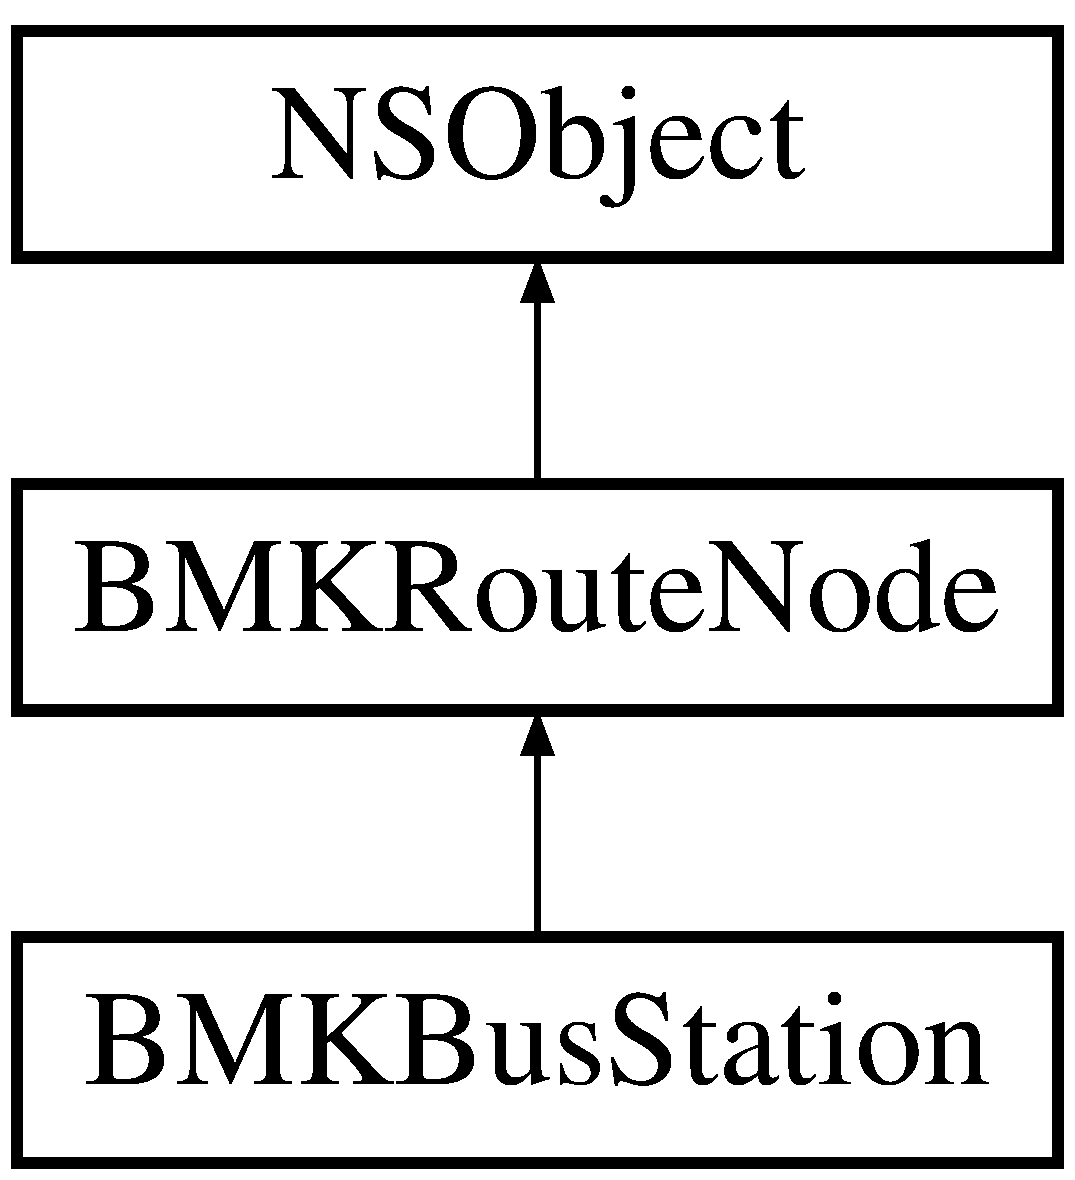
\includegraphics[height=3.000000cm]{interface_b_m_k_bus_station}
\end{center}
\end{figure}
\subsection*{额外继承的成员函数}


\subsection{详细描述}
此类表示公交站点信息 

该类的文档由以下文件生成\+:\begin{DoxyCompactItemize}
\item 
output/map\+\_\+search\+\_\+cloud\+\_\+loc\+\_\+util/inc/B\+M\+K\+Route\+Search\+Type.\+h\end{DoxyCompactItemize}

\hypertarget{interface_b_m_k_bus_step}{\section{B\+M\+K\+Bus\+Step类 参考}
\label{interface_b_m_k_bus_step}\index{B\+M\+K\+Bus\+Step@{B\+M\+K\+Bus\+Step}}
}


此类表示公交线路中的一个路段  




{\ttfamily \#import $<$B\+M\+K\+Route\+Search\+Type.\+h$>$}

类 B\+M\+K\+Bus\+Step 继承关系图\+:\begin{figure}[H]
\begin{center}
\leavevmode
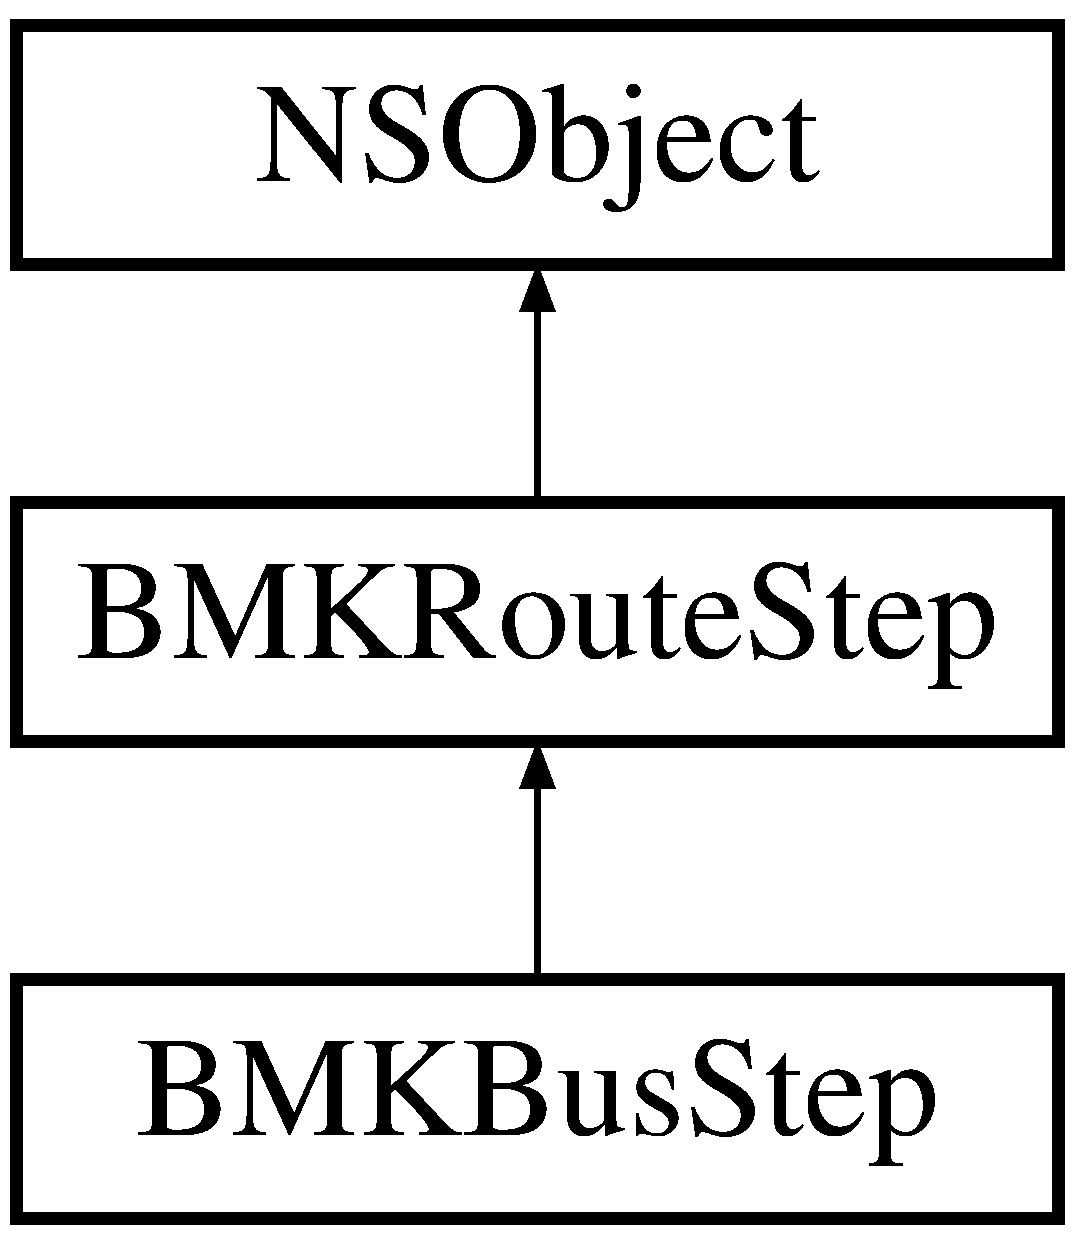
\includegraphics[height=3.000000cm]{interface_b_m_k_bus_step}
\end{center}
\end{figure}
\subsection*{额外继承的成员函数}


\subsection{详细描述}
此类表示公交线路中的一个路段 

该类的文档由以下文件生成\+:\begin{DoxyCompactItemize}
\item 
output/map\+\_\+search\+\_\+cloud\+\_\+loc\+\_\+util/inc/B\+M\+K\+Route\+Search\+Type.\+h\end{DoxyCompactItemize}

\hypertarget{interface_b_m_k_circle}{\section{B\+M\+K\+Circle类 参考}
\label{interface_b_m_k_circle}\index{B\+M\+K\+Circle@{B\+M\+K\+Circle}}
}


该类用于定义一个圆  




{\ttfamily \#import $<$B\+M\+K\+Circle.\+h$>$}

类 B\+M\+K\+Circle 继承关系图\+:\begin{figure}[H]
\begin{center}
\leavevmode
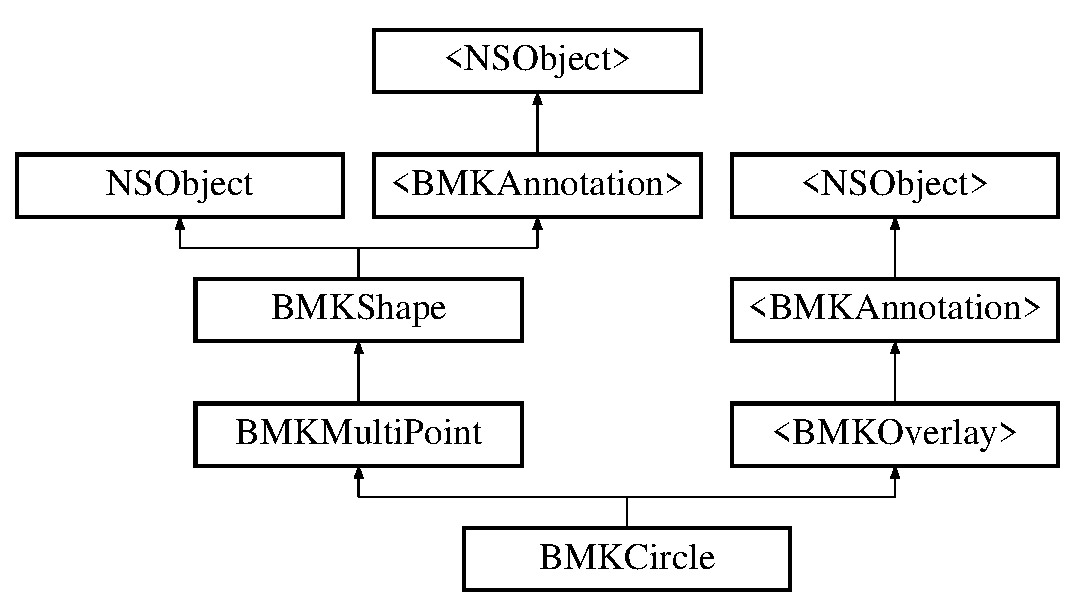
\includegraphics[height=5.000000cm]{interface_b_m_k_circle}
\end{center}
\end{figure}
\subsection*{Class Methods}
\begin{DoxyCompactItemize}
\item 
(\hyperlink{interface_b_m_k_circle}{B\+M\+K\+Circle} $\ast$) + \hyperlink{interface_b_m_k_circle_a82a7234e92fda719b74d6055ee30d360}{circle\+With\+Center\+Coordinate\+:radius\+:}
\item 
(\hyperlink{interface_b_m_k_circle}{B\+M\+K\+Circle} $\ast$) + \hyperlink{interface_b_m_k_circle_af4109f36f784b80a758a0b48c636e4a7}{circle\+With\+Map\+Rect\+:}
\end{DoxyCompactItemize}
\subsection*{Protected 属性}
\begin{DoxyCompactItemize}
\item 
\hypertarget{interface_b_m_k_circle_a2dffabfbaa1ac6642adc5a475d6ee453}{package B\+O\+O\+L {\bfseries \+\_\+invalidate}}\label{interface_b_m_k_circle_a2dffabfbaa1ac6642adc5a475d6ee453}

\item 
\hypertarget{interface_b_m_k_circle_abdd404f22d461b81d8d4d203778cee58}{C\+L\+Location\+Coordinate2\+D {\bfseries \+\_\+coordinate}}\label{interface_b_m_k_circle_abdd404f22d461b81d8d4d203778cee58}

\item 
\hypertarget{interface_b_m_k_circle_a84860dbbaa96509cfa4c7590908aabe8}{C\+L\+Location\+Distance {\bfseries \+\_\+radius}}\label{interface_b_m_k_circle_a84860dbbaa96509cfa4c7590908aabe8}

\item 
\hypertarget{interface_b_m_k_circle_abfa42e25c856dd426fb74b9531e1061b}{\hyperlink{struct_b_m_k_map_rect}{B\+M\+K\+Map\+Rect} {\bfseries \+\_\+bounding\+Map\+Rect}}\label{interface_b_m_k_circle_abfa42e25c856dd426fb74b9531e1061b}

\end{DoxyCompactItemize}
\subsection*{属性}
\begin{DoxyCompactItemize}
\item 
\hypertarget{interface_b_m_k_circle_a1c516c10dec1971c686e07f814f333f9}{C\+L\+Location\+Coordinate2\+D \hyperlink{interface_b_m_k_circle_a1c516c10dec1971c686e07f814f333f9}{coordinate}}\label{interface_b_m_k_circle_a1c516c10dec1971c686e07f814f333f9}

\begin{DoxyCompactList}\small\item\em 中心点坐标 \end{DoxyCompactList}\item 
\hypertarget{interface_b_m_k_circle_a42507e4c17b4a1c1309fcbe06e370bf5}{C\+L\+Location\+Distance \hyperlink{interface_b_m_k_circle_a42507e4c17b4a1c1309fcbe06e370bf5}{radius}}\label{interface_b_m_k_circle_a42507e4c17b4a1c1309fcbe06e370bf5}

\begin{DoxyCompactList}\small\item\em 半径,单位:米 \end{DoxyCompactList}\item 
\hypertarget{interface_b_m_k_circle_a462a1696e47b1523dd481b22d43bcf46}{\hyperlink{struct_b_m_k_map_rect}{B\+M\+K\+Map\+Rect} \hyperlink{interface_b_m_k_circle_a462a1696e47b1523dd481b22d43bcf46}{bounding\+Map\+Rect}}\label{interface_b_m_k_circle_a462a1696e47b1523dd481b22d43bcf46}

\begin{DoxyCompactList}\small\item\em 该圆的外接矩形 \end{DoxyCompactList}\end{DoxyCompactItemize}
\subsection*{额外继承的成员函数}


\subsection{详细描述}
该类用于定义一个圆 

\subsection{Method Documentation}
\hypertarget{interface_b_m_k_circle_a82a7234e92fda719b74d6055ee30d360}{\index{B\+M\+K\+Circle@{B\+M\+K\+Circle}!circle\+With\+Center\+Coordinate\+:radius\+:@{circle\+With\+Center\+Coordinate\+:radius\+:}}
\index{circle\+With\+Center\+Coordinate\+:radius\+:@{circle\+With\+Center\+Coordinate\+:radius\+:}!B\+M\+K\+Circle@{B\+M\+K\+Circle}}
\subsubsection[{circle\+With\+Center\+Coordinate\+:radius\+:}]{\setlength{\rightskip}{0pt plus 5cm}+ ({\bf B\+M\+K\+Circle} $\ast$) circle\+With\+Center\+Coordinate\+: 
\begin{DoxyParamCaption}
\item[{(C\+L\+Location\+Coordinate2\+D)}]{coord}
\item[{radius:(C\+L\+Location\+Distance)}]{radius}
\end{DoxyParamCaption}
}}\label{interface_b_m_k_circle_a82a7234e92fda719b74d6055ee30d360}
根据中心点和半径生成圆 
\begin{DoxyParams}{参数}
{\em coord} & 中心点的经纬度坐标 \\
\hline
{\em radius} & 半径,单位:米 \\
\hline
\end{DoxyParams}
\begin{DoxyReturn}{返回}
新生成的圆 
\end{DoxyReturn}
\hypertarget{interface_b_m_k_circle_af4109f36f784b80a758a0b48c636e4a7}{\index{B\+M\+K\+Circle@{B\+M\+K\+Circle}!circle\+With\+Map\+Rect\+:@{circle\+With\+Map\+Rect\+:}}
\index{circle\+With\+Map\+Rect\+:@{circle\+With\+Map\+Rect\+:}!B\+M\+K\+Circle@{B\+M\+K\+Circle}}
\subsubsection[{circle\+With\+Map\+Rect\+:}]{\setlength{\rightskip}{0pt plus 5cm}+ ({\bf B\+M\+K\+Circle} $\ast$) circle\+With\+Map\+Rect\+: 
\begin{DoxyParamCaption}
\item[{({\bf B\+M\+K\+Map\+Rect})}]{map\+Rect}
\end{DoxyParamCaption}
}}\label{interface_b_m_k_circle_af4109f36f784b80a758a0b48c636e4a7}
根据指定的直角坐标矩形生成圆,半径由较长的那条边决定,radius = M\+A\+X(width, height)/2 
\begin{DoxyParams}{参数}
{\em map\+Rect} & 指定的直角坐标矩形 \\
\hline
\end{DoxyParams}
\begin{DoxyReturn}{返回}
新生成的圆 
\end{DoxyReturn}


该类的文档由以下文件生成\+:\begin{DoxyCompactItemize}
\item 
output/map\+\_\+search\+\_\+cloud\+\_\+loc\+\_\+util/inc/B\+M\+K\+Circle.\+h\end{DoxyCompactItemize}

\hypertarget{interface_b_m_k_circle_view}{\section{B\+M\+K\+Circle\+View类 参考}
\label{interface_b_m_k_circle_view}\index{B\+M\+K\+Circle\+View@{B\+M\+K\+Circle\+View}}
}


该类用于定义圆对应的\+View  




{\ttfamily \#import $<$B\+M\+K\+Circle\+View.\+h$>$}

类 B\+M\+K\+Circle\+View 继承关系图\+:\begin{figure}[H]
\begin{center}
\leavevmode
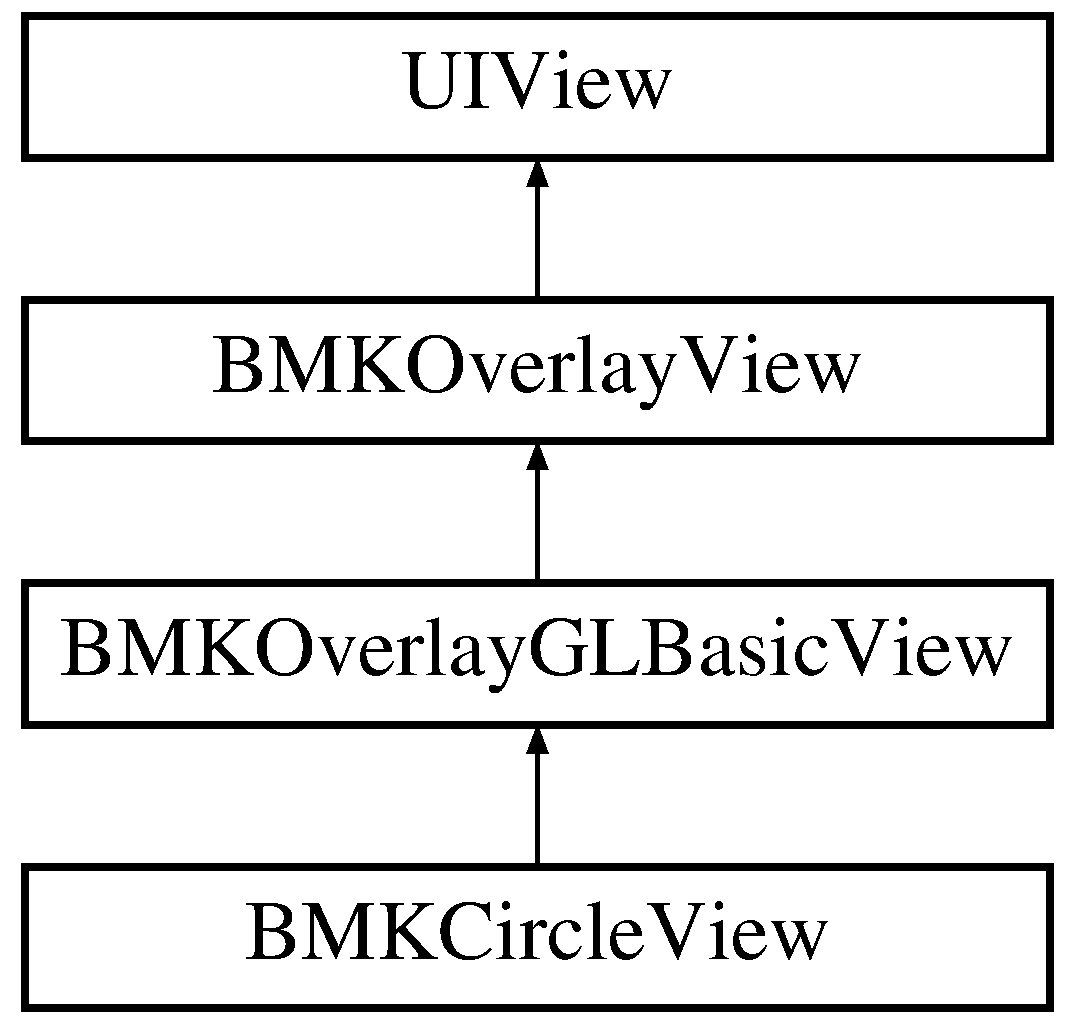
\includegraphics[height=4.000000cm]{interface_b_m_k_circle_view}
\end{center}
\end{figure}
\subsection*{Instance Methods}
\begin{DoxyCompactItemize}
\item 
(id) -\/ \hyperlink{interface_b_m_k_circle_view_a35f06526cf5423a39d434edc0517d34e}{init\+With\+Circle\+:}
\end{DoxyCompactItemize}
\subsection*{属性}
\begin{DoxyCompactItemize}
\item 
\hypertarget{interface_b_m_k_circle_view_a07fe8c131d40bb225849dbc9bfb17e18}{\hyperlink{interface_b_m_k_circle}{B\+M\+K\+Circle} $\ast$ \hyperlink{interface_b_m_k_circle_view_a07fe8c131d40bb225849dbc9bfb17e18}{circle}}\label{interface_b_m_k_circle_view_a07fe8c131d40bb225849dbc9bfb17e18}

\begin{DoxyCompactList}\small\item\em 该\+View对应的圆 \end{DoxyCompactList}\end{DoxyCompactItemize}
\subsection*{额外继承的成员函数}


\subsection{详细描述}
该类用于定义圆对应的\+View 

\subsection{Method Documentation}
\hypertarget{interface_b_m_k_circle_view_a35f06526cf5423a39d434edc0517d34e}{\index{B\+M\+K\+Circle\+View@{B\+M\+K\+Circle\+View}!init\+With\+Circle\+:@{init\+With\+Circle\+:}}
\index{init\+With\+Circle\+:@{init\+With\+Circle\+:}!B\+M\+K\+Circle\+View@{B\+M\+K\+Circle\+View}}
\subsubsection[{init\+With\+Circle\+:}]{\setlength{\rightskip}{0pt plus 5cm}-\/ (id) init\+With\+Circle\+: 
\begin{DoxyParamCaption}
\item[{({\bf B\+M\+K\+Circle} $\ast$)}]{circle}
\end{DoxyParamCaption}
}}\label{interface_b_m_k_circle_view_a35f06526cf5423a39d434edc0517d34e}
根据指定圆生成对应的\+View 
\begin{DoxyParams}{参数}
{\em circle} & 指定的圆 \\
\hline
\end{DoxyParams}
\begin{DoxyReturn}{返回}
生成的\+View 
\end{DoxyReturn}


该类的文档由以下文件生成\+:\begin{DoxyCompactItemize}
\item 
output/map\+\_\+search\+\_\+cloud\+\_\+loc\+\_\+util/inc/B\+M\+K\+Circle\+View.\+h\end{DoxyCompactItemize}

\hypertarget{interface_b_m_k_city_list_info}{\section{B\+M\+K\+City\+List\+Info类 参考}
\label{interface_b_m_k_city_list_info}\index{B\+M\+K\+City\+List\+Info@{B\+M\+K\+City\+List\+Info}}
}


城市列表信息类  




{\ttfamily \#import $<$B\+M\+K\+Poi\+Search\+Type.\+h$>$}

类 B\+M\+K\+City\+List\+Info 继承关系图\+:\begin{figure}[H]
\begin{center}
\leavevmode
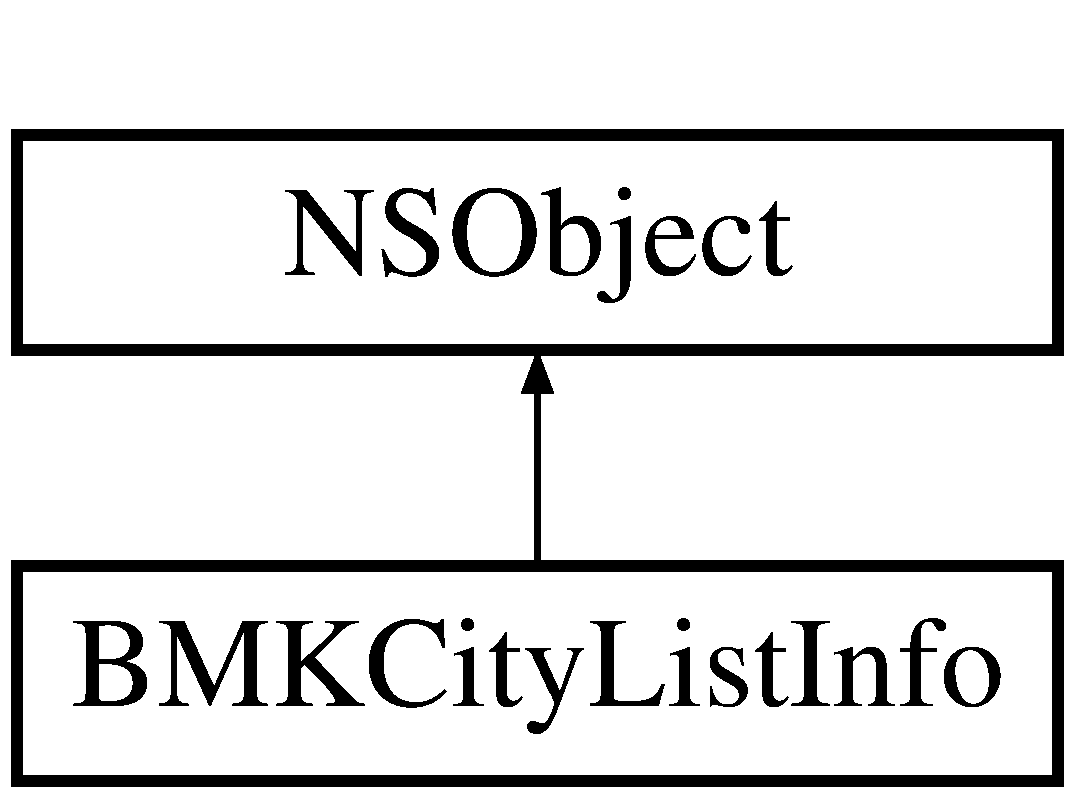
\includegraphics[height=2.000000cm]{interface_b_m_k_city_list_info}
\end{center}
\end{figure}
\subsection*{Protected 属性}
\begin{DoxyCompactItemize}
\item 
\hypertarget{interface_b_m_k_city_list_info_a868f1df35a24867c0957420506703225}{N\+S\+String $\ast$ {\bfseries \+\_\+city}}\label{interface_b_m_k_city_list_info_a868f1df35a24867c0957420506703225}

\item 
\hypertarget{interface_b_m_k_city_list_info_a0cc9abd0bfad17b52c924611f975db77}{int {\bfseries \+\_\+num}}\label{interface_b_m_k_city_list_info_a0cc9abd0bfad17b52c924611f975db77}

\end{DoxyCompactItemize}
\subsection*{属性}
\begin{DoxyCompactItemize}
\item 
\hypertarget{interface_b_m_k_city_list_info_ad1b2093344ad0524a9bef93c823f8242}{N\+S\+String $\ast$ \hyperlink{interface_b_m_k_city_list_info_ad1b2093344ad0524a9bef93c823f8242}{city}}\label{interface_b_m_k_city_list_info_ad1b2093344ad0524a9bef93c823f8242}

\begin{DoxyCompactList}\small\item\em 城市名称 \end{DoxyCompactList}\item 
\hypertarget{interface_b_m_k_city_list_info_a63163c524339e1687d90541b3a24b54c}{int \hyperlink{interface_b_m_k_city_list_info_a63163c524339e1687d90541b3a24b54c}{num}}\label{interface_b_m_k_city_list_info_a63163c524339e1687d90541b3a24b54c}

\begin{DoxyCompactList}\small\item\em 该城市所含搜索结果数目 \end{DoxyCompactList}\end{DoxyCompactItemize}


\subsection{详细描述}
城市列表信息类 

该类的文档由以下文件生成\+:\begin{DoxyCompactItemize}
\item 
output/map\+\_\+search\+\_\+cloud\+\_\+loc\+\_\+util/inc/B\+M\+K\+Poi\+Search\+Type.\+h\end{DoxyCompactItemize}

\hypertarget{interface_b_m_k_city_search_option}{\section{B\+M\+K\+City\+Search\+Option类 参考}
\label{interface_b_m_k_city_search_option}\index{B\+M\+K\+City\+Search\+Option@{B\+M\+K\+City\+Search\+Option}}
}


本地云检索参数信息类  




{\ttfamily \#import $<$B\+M\+K\+Poi\+Search\+Option.\+h$>$}

类 B\+M\+K\+City\+Search\+Option 继承关系图\+:\begin{figure}[H]
\begin{center}
\leavevmode
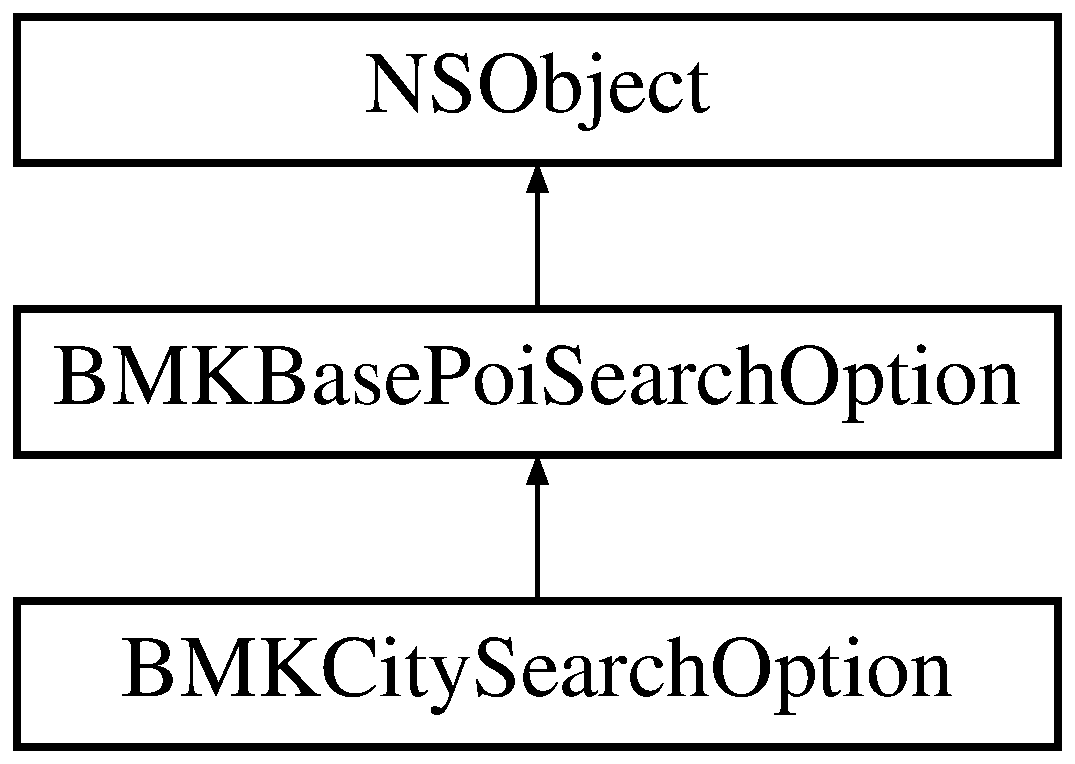
\includegraphics[height=3.000000cm]{interface_b_m_k_city_search_option}
\end{center}
\end{figure}
\subsection*{Protected 属性}
\begin{DoxyCompactItemize}
\item 
\hypertarget{interface_b_m_k_city_search_option_a6d14cd2f7fcac7cd601ef9bfd0439720}{N\+S\+String $\ast$ {\bfseries \+\_\+city}}\label{interface_b_m_k_city_search_option_a6d14cd2f7fcac7cd601ef9bfd0439720}

\end{DoxyCompactItemize}
\subsection*{属性}
\begin{DoxyCompactItemize}
\item 
\hypertarget{interface_b_m_k_city_search_option_af9e2e37c3edcd43445f58660e770f8b1}{N\+S\+String $\ast$ \hyperlink{interface_b_m_k_city_search_option_af9e2e37c3edcd43445f58660e770f8b1}{city}}\label{interface_b_m_k_city_search_option_af9e2e37c3edcd43445f58660e770f8b1}

\begin{DoxyCompactList}\small\item\em 区域名称(市或区的名字,如北京市,海淀区),必选, 必须最长25个字符 \end{DoxyCompactList}\end{DoxyCompactItemize}


\subsection{详细描述}
本地云检索参数信息类 

该类的文档由以下文件生成\+:\begin{DoxyCompactItemize}
\item 
output/map\+\_\+search\+\_\+cloud\+\_\+loc\+\_\+util/inc/B\+M\+K\+Poi\+Search\+Option.\+h\end{DoxyCompactItemize}

\hypertarget{interface_b_m_k_cloud_bound_search_info}{\section{B\+M\+K\+Cloud\+Bound\+Search\+Info类 参考}
\label{interface_b_m_k_cloud_bound_search_info}\index{B\+M\+K\+Cloud\+Bound\+Search\+Info@{B\+M\+K\+Cloud\+Bound\+Search\+Info}}
}


矩形云检索参数信息类  




{\ttfamily \#import $<$B\+M\+K\+Cloud\+Search\+Info.\+h$>$}

类 B\+M\+K\+Cloud\+Bound\+Search\+Info 继承关系图\+:\begin{figure}[H]
\begin{center}
\leavevmode
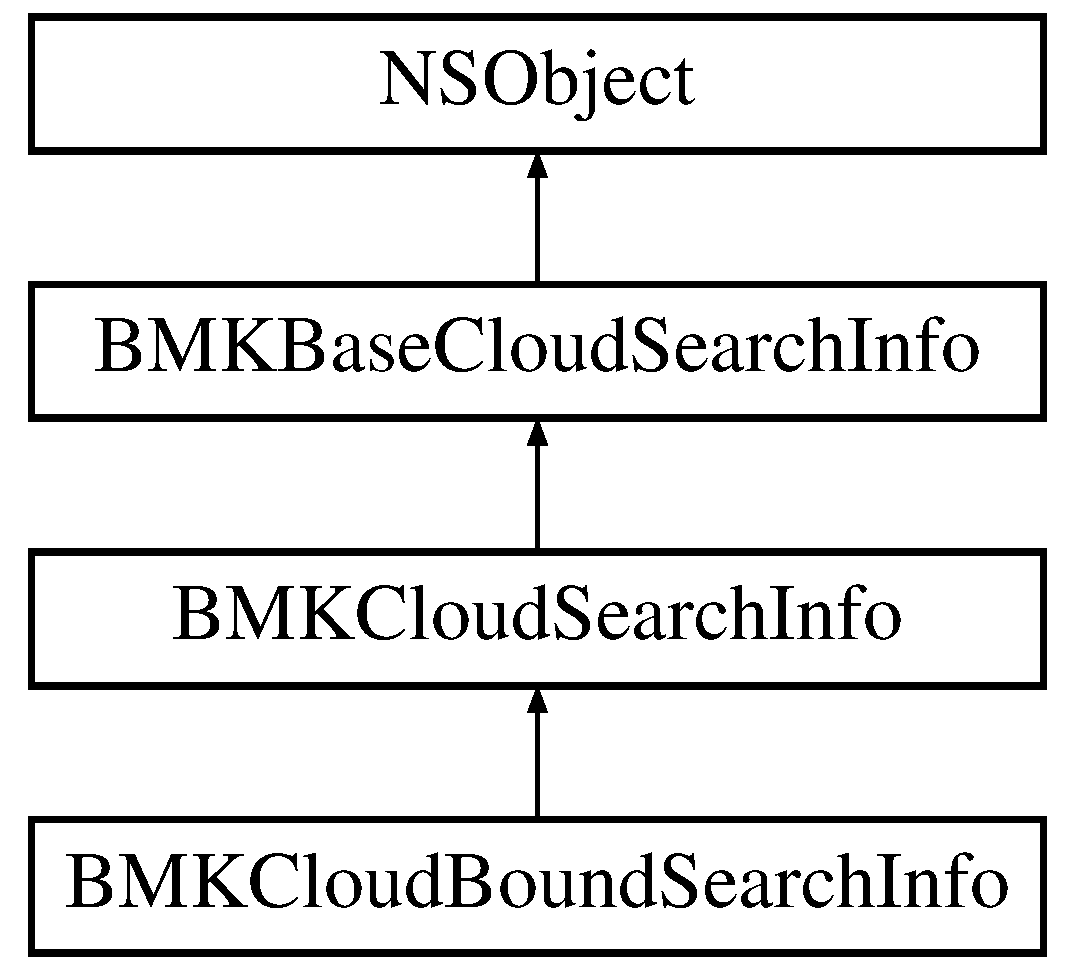
\includegraphics[height=4.000000cm]{interface_b_m_k_cloud_bound_search_info}
\end{center}
\end{figure}
\subsection*{Protected 属性}
\begin{DoxyCompactItemize}
\item 
\hypertarget{interface_b_m_k_cloud_bound_search_info_aab508b50d538d64dbd6e45d3280aa1d9}{N\+S\+String $\ast$ {\bfseries \+\_\+bounds}}\label{interface_b_m_k_cloud_bound_search_info_aab508b50d538d64dbd6e45d3280aa1d9}

\end{DoxyCompactItemize}
\subsection*{属性}
\begin{DoxyCompactItemize}
\item 
\hypertarget{interface_b_m_k_cloud_bound_search_info_a23623d581d1b1e81766d9c46048966cb}{N\+S\+String $\ast$ \hyperlink{interface_b_m_k_cloud_bound_search_info_a23623d581d1b1e81766d9c46048966cb}{bounds}}\label{interface_b_m_k_cloud_bound_search_info_a23623d581d1b1e81766d9c46048966cb}

\begin{DoxyCompactList}\small\item\em 矩形区域,左下角和右上角的经纬度坐标点。2个点用;号分隔(116.\+30,36.\+20;117.\+30,37.\+20),string(25) \end{DoxyCompactList}\end{DoxyCompactItemize}


\subsection{详细描述}
矩形云检索参数信息类 

该类的文档由以下文件生成\+:\begin{DoxyCompactItemize}
\item 
output/map\+\_\+search\+\_\+cloud\+\_\+loc\+\_\+util/inc/B\+M\+K\+Cloud\+Search\+Info.\+h\end{DoxyCompactItemize}

\hypertarget{interface_b_m_k_cloud_detail_search_info}{\section{B\+M\+K\+Cloud\+Detail\+Search\+Info类 参考}
\label{interface_b_m_k_cloud_detail_search_info}\index{B\+M\+K\+Cloud\+Detail\+Search\+Info@{B\+M\+K\+Cloud\+Detail\+Search\+Info}}
}


详情云检索参数信息类  




{\ttfamily \#import $<$B\+M\+K\+Cloud\+Search\+Info.\+h$>$}

类 B\+M\+K\+Cloud\+Detail\+Search\+Info 继承关系图\+:\begin{figure}[H]
\begin{center}
\leavevmode
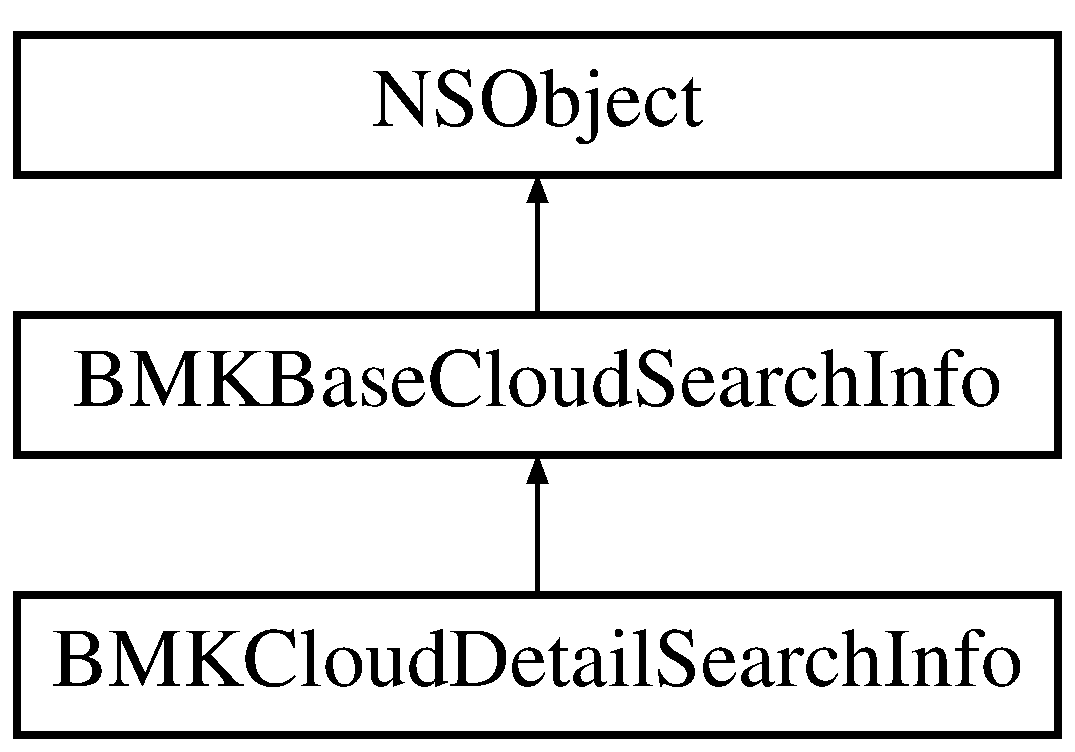
\includegraphics[height=3.000000cm]{interface_b_m_k_cloud_detail_search_info}
\end{center}
\end{figure}
\subsection*{Protected 属性}
\begin{DoxyCompactItemize}
\item 
\hypertarget{interface_b_m_k_cloud_detail_search_info_af0561e1d6ce5656002bb7b576ac51b4f}{N\+S\+String $\ast$ {\bfseries \+\_\+uid}}\label{interface_b_m_k_cloud_detail_search_info_af0561e1d6ce5656002bb7b576ac51b4f}

\end{DoxyCompactItemize}
\subsection*{属性}
\begin{DoxyCompactItemize}
\item 
\hypertarget{interface_b_m_k_cloud_detail_search_info_ad553991a75b6d30409a9d3525bea9c52}{N\+S\+String $\ast$ \hyperlink{interface_b_m_k_cloud_detail_search_info_ad553991a75b6d30409a9d3525bea9c52}{uid}}\label{interface_b_m_k_cloud_detail_search_info_ad553991a75b6d30409a9d3525bea9c52}

\begin{DoxyCompactList}\small\item\em uid为poi点的id值 \end{DoxyCompactList}\end{DoxyCompactItemize}


\subsection{详细描述}
详情云检索参数信息类 

该类的文档由以下文件生成\+:\begin{DoxyCompactItemize}
\item 
output/map\+\_\+search\+\_\+cloud\+\_\+loc\+\_\+util/inc/B\+M\+K\+Cloud\+Search\+Info.\+h\end{DoxyCompactItemize}

\hypertarget{interface_b_m_k_cloud_local_search_info}{\section{B\+M\+K\+Cloud\+Local\+Search\+Info类 参考}
\label{interface_b_m_k_cloud_local_search_info}\index{B\+M\+K\+Cloud\+Local\+Search\+Info@{B\+M\+K\+Cloud\+Local\+Search\+Info}}
}


本地云检索参数信息类  




{\ttfamily \#import $<$B\+M\+K\+Cloud\+Search\+Info.\+h$>$}

类 B\+M\+K\+Cloud\+Local\+Search\+Info 继承关系图\+:\begin{figure}[H]
\begin{center}
\leavevmode
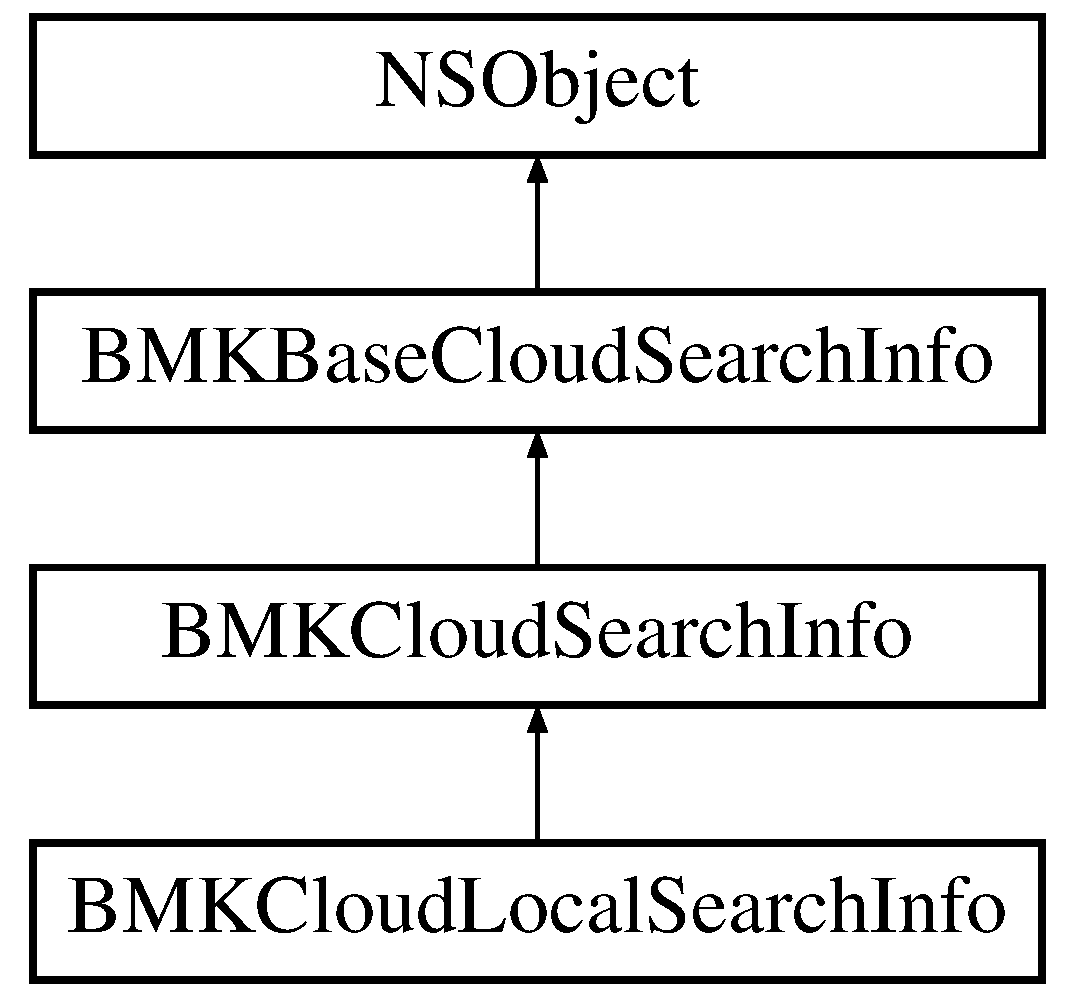
\includegraphics[height=4.000000cm]{interface_b_m_k_cloud_local_search_info}
\end{center}
\end{figure}
\subsection*{Protected 属性}
\begin{DoxyCompactItemize}
\item 
\hypertarget{interface_b_m_k_cloud_local_search_info_a222e06088269c5b3e67d3f9a416d7eff}{N\+S\+String $\ast$ {\bfseries \+\_\+region}}\label{interface_b_m_k_cloud_local_search_info_a222e06088269c5b3e67d3f9a416d7eff}

\end{DoxyCompactItemize}
\subsection*{属性}
\begin{DoxyCompactItemize}
\item 
\hypertarget{interface_b_m_k_cloud_local_search_info_a0f5a080b5eed8356479c5b3f3e483e29}{N\+S\+String $\ast$ \hyperlink{interface_b_m_k_cloud_local_search_info_a0f5a080b5eed8356479c5b3f3e483e29}{region}}\label{interface_b_m_k_cloud_local_search_info_a0f5a080b5eed8356479c5b3f3e483e29}

\begin{DoxyCompactList}\small\item\em 区域名称(市或区的名字,如北京市,海淀区),必选, 必须最长25个字符 \end{DoxyCompactList}\end{DoxyCompactItemize}


\subsection{详细描述}
本地云检索参数信息类 

该类的文档由以下文件生成\+:\begin{DoxyCompactItemize}
\item 
output/map\+\_\+search\+\_\+cloud\+\_\+loc\+\_\+util/inc/B\+M\+K\+Cloud\+Search\+Info.\+h\end{DoxyCompactItemize}

\hypertarget{interface_b_m_k_cloud_nearby_search_info}{\section{B\+M\+K\+Cloud\+Nearby\+Search\+Info类 参考}
\label{interface_b_m_k_cloud_nearby_search_info}\index{B\+M\+K\+Cloud\+Nearby\+Search\+Info@{B\+M\+K\+Cloud\+Nearby\+Search\+Info}}
}


周边云检索参数信息类  




{\ttfamily \#import $<$B\+M\+K\+Cloud\+Search\+Info.\+h$>$}

类 B\+M\+K\+Cloud\+Nearby\+Search\+Info 继承关系图\+:\begin{figure}[H]
\begin{center}
\leavevmode
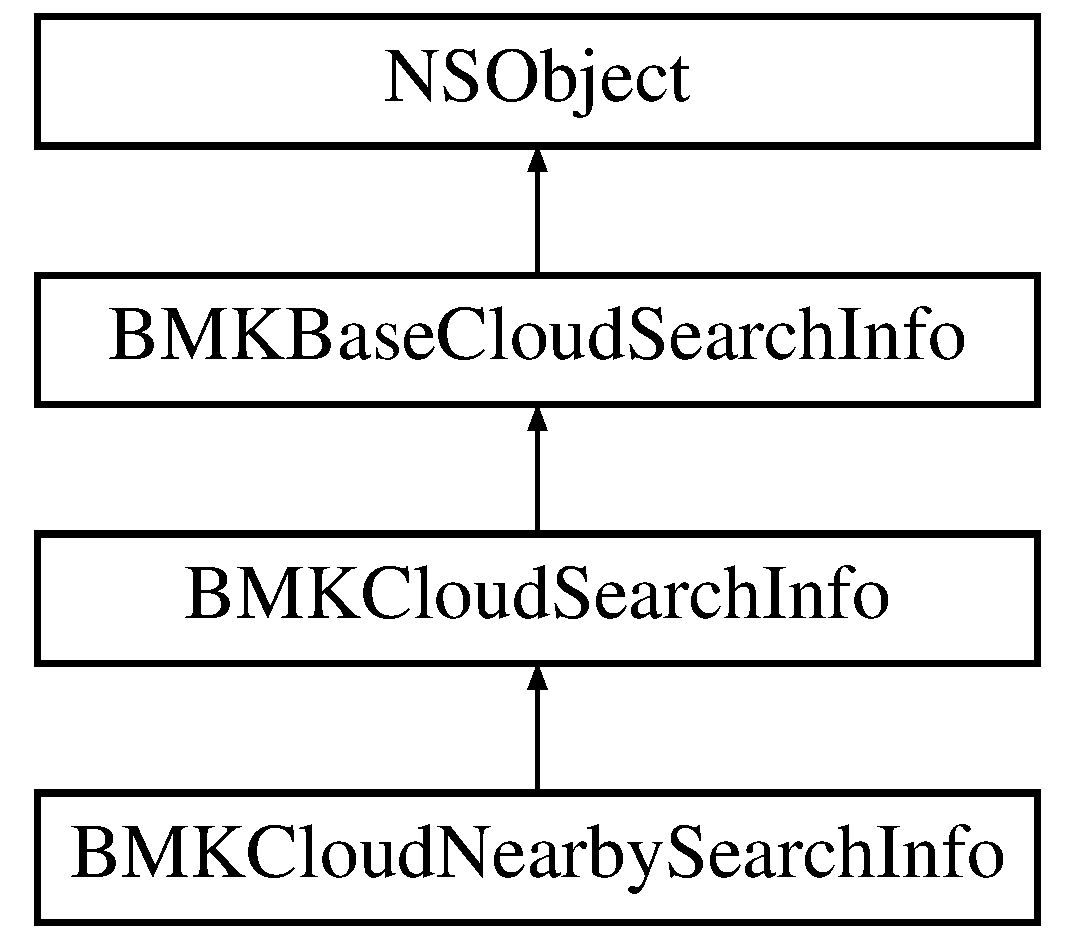
\includegraphics[height=4.000000cm]{interface_b_m_k_cloud_nearby_search_info}
\end{center}
\end{figure}
\subsection*{Protected 属性}
\begin{DoxyCompactItemize}
\item 
\hypertarget{interface_b_m_k_cloud_nearby_search_info_a6a4cfe0d1809afeaa9f9fd78bb29ded3}{N\+S\+String $\ast$ {\bfseries \+\_\+location}}\label{interface_b_m_k_cloud_nearby_search_info_a6a4cfe0d1809afeaa9f9fd78bb29ded3}

\item 
\hypertarget{interface_b_m_k_cloud_nearby_search_info_a30c18210f666d7913e3f8d9c00161016}{int {\bfseries \+\_\+radius}}\label{interface_b_m_k_cloud_nearby_search_info_a30c18210f666d7913e3f8d9c00161016}

\end{DoxyCompactItemize}
\subsection*{属性}
\begin{DoxyCompactItemize}
\item 
\hypertarget{interface_b_m_k_cloud_nearby_search_info_ae129357a1f589b69f9a2f8ca3613f015}{N\+S\+String $\ast$ \hyperlink{interface_b_m_k_cloud_nearby_search_info_ae129357a1f589b69f9a2f8ca3613f015}{location}}\label{interface_b_m_k_cloud_nearby_search_info_ae129357a1f589b69f9a2f8ca3613f015}

\begin{DoxyCompactList}\small\item\em 检索的中心点,逗号分隔的经纬度(116.\+4321,38.\+76623),string(25) \end{DoxyCompactList}\item 
\hypertarget{interface_b_m_k_cloud_nearby_search_info_af736625a3a921ec13dd0c8a6deb1c52f}{int \hyperlink{interface_b_m_k_cloud_nearby_search_info_af736625a3a921ec13dd0c8a6deb1c52f}{radius}}\label{interface_b_m_k_cloud_nearby_search_info_af736625a3a921ec13dd0c8a6deb1c52f}

\begin{DoxyCompactList}\small\item\em 周边检索半径 \end{DoxyCompactList}\end{DoxyCompactItemize}


\subsection{详细描述}
周边云检索参数信息类 

该类的文档由以下文件生成\+:\begin{DoxyCompactItemize}
\item 
output/map\+\_\+search\+\_\+cloud\+\_\+loc\+\_\+util/inc/B\+M\+K\+Cloud\+Search\+Info.\+h\end{DoxyCompactItemize}

\hypertarget{interface_b_m_k_cloud_p_o_i_info}{\section{B\+M\+K\+Cloud\+P\+O\+I\+Info类 参考}
\label{interface_b_m_k_cloud_p_o_i_info}\index{B\+M\+K\+Cloud\+P\+O\+I\+Info@{B\+M\+K\+Cloud\+P\+O\+I\+Info}}
}


云检索结果信息类  




{\ttfamily \#import $<$B\+M\+K\+Cloud\+P\+O\+I\+List.\+h$>$}

类 B\+M\+K\+Cloud\+P\+O\+I\+Info 继承关系图\+:\begin{figure}[H]
\begin{center}
\leavevmode
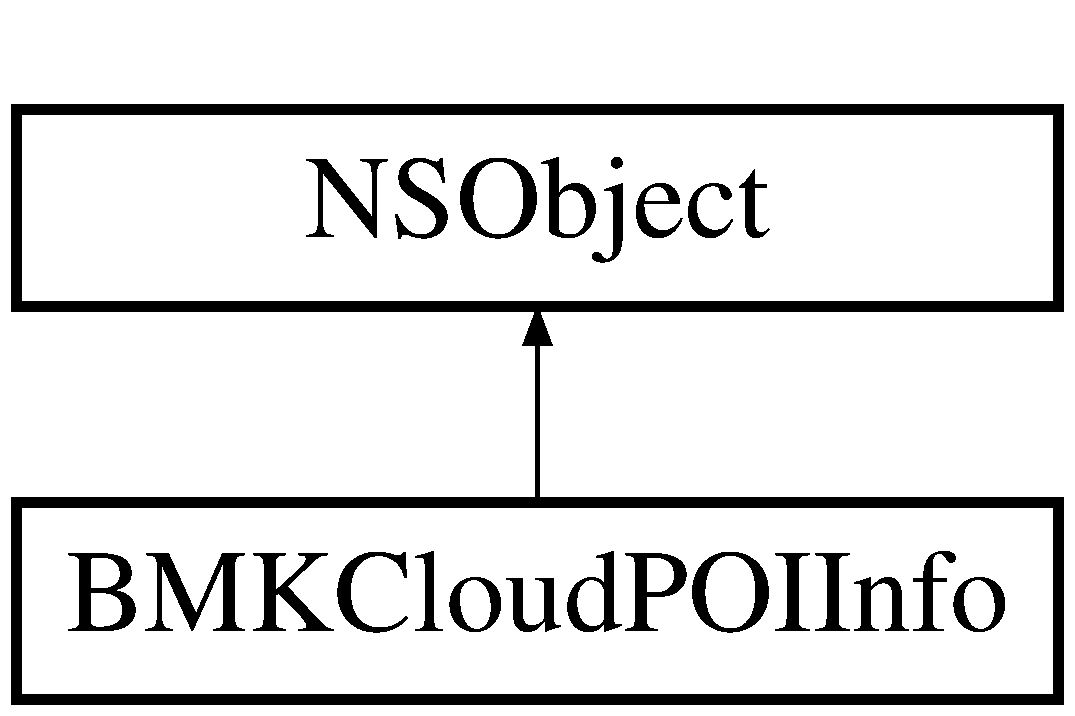
\includegraphics[height=2.000000cm]{interface_b_m_k_cloud_p_o_i_info}
\end{center}
\end{figure}
\subsection*{Protected 属性}
\begin{DoxyCompactItemize}
\item 
\hypertarget{interface_b_m_k_cloud_p_o_i_info_a15045f4a4be1416b93e05c60e28a4c1b}{int {\bfseries \+\_\+uid}}\label{interface_b_m_k_cloud_p_o_i_info_a15045f4a4be1416b93e05c60e28a4c1b}

\item 
\hypertarget{interface_b_m_k_cloud_p_o_i_info_a82a894e1d15daf69a52da80f7ef3ea6a}{int {\bfseries \+\_\+geotable\+Id}}\label{interface_b_m_k_cloud_p_o_i_info_a82a894e1d15daf69a52da80f7ef3ea6a}

\item 
\hypertarget{interface_b_m_k_cloud_p_o_i_info_ab96b69fa322abff5474318fc83e1b5b2}{N\+S\+String $\ast$ {\bfseries \+\_\+title}}\label{interface_b_m_k_cloud_p_o_i_info_ab96b69fa322abff5474318fc83e1b5b2}

\item 
\hypertarget{interface_b_m_k_cloud_p_o_i_info_a041ca0932012f892d436909b43104e65}{N\+S\+String $\ast$ {\bfseries \+\_\+address}}\label{interface_b_m_k_cloud_p_o_i_info_a041ca0932012f892d436909b43104e65}

\item 
\hypertarget{interface_b_m_k_cloud_p_o_i_info_adae710495f2b8898af9ca1c773cb0d81}{N\+S\+String $\ast$ {\bfseries \+\_\+province}}\label{interface_b_m_k_cloud_p_o_i_info_adae710495f2b8898af9ca1c773cb0d81}

\item 
\hypertarget{interface_b_m_k_cloud_p_o_i_info_af6ae3d92e14c0ed11910700087fa296c}{N\+S\+String $\ast$ {\bfseries \+\_\+city}}\label{interface_b_m_k_cloud_p_o_i_info_af6ae3d92e14c0ed11910700087fa296c}

\item 
\hypertarget{interface_b_m_k_cloud_p_o_i_info_a5b28b645901af1799733d068bfdb0168}{N\+S\+String $\ast$ {\bfseries \+\_\+district}}\label{interface_b_m_k_cloud_p_o_i_info_a5b28b645901af1799733d068bfdb0168}

\item 
\hypertarget{interface_b_m_k_cloud_p_o_i_info_a8216e102a0ea3efd4e9b0c4e74888eee}{float {\bfseries \+\_\+latitude}}\label{interface_b_m_k_cloud_p_o_i_info_a8216e102a0ea3efd4e9b0c4e74888eee}

\item 
\hypertarget{interface_b_m_k_cloud_p_o_i_info_ab6025818e05241d008964c322a92b59f}{float {\bfseries \+\_\+longitude}}\label{interface_b_m_k_cloud_p_o_i_info_ab6025818e05241d008964c322a92b59f}

\item 
\hypertarget{interface_b_m_k_cloud_p_o_i_info_a7a918dcc5736a1e5cb4077000e9f4762}{N\+S\+String $\ast$ {\bfseries \+\_\+tags}}\label{interface_b_m_k_cloud_p_o_i_info_a7a918dcc5736a1e5cb4077000e9f4762}

\item 
\hypertarget{interface_b_m_k_cloud_p_o_i_info_aa72375b226a48c5c1b764da84e234acd}{float {\bfseries \+\_\+distance}}\label{interface_b_m_k_cloud_p_o_i_info_aa72375b226a48c5c1b764da84e234acd}

\item 
\hypertarget{interface_b_m_k_cloud_p_o_i_info_ae1e73b90bd2948218f37c4c1c065c68e}{float {\bfseries \+\_\+weight}}\label{interface_b_m_k_cloud_p_o_i_info_ae1e73b90bd2948218f37c4c1c065c68e}

\item 
\hypertarget{interface_b_m_k_cloud_p_o_i_info_a8a653bb3edd7997f7597a536a0dfd2b8}{N\+S\+Mutable\+Dictionary $\ast$ {\bfseries \+\_\+custom\+Dict}}\label{interface_b_m_k_cloud_p_o_i_info_a8a653bb3edd7997f7597a536a0dfd2b8}

\item 
\hypertarget{interface_b_m_k_cloud_p_o_i_info_a50b88f009188671372e5e49737316723}{int {\bfseries \+\_\+creattime}}\label{interface_b_m_k_cloud_p_o_i_info_a50b88f009188671372e5e49737316723}

\item 
\hypertarget{interface_b_m_k_cloud_p_o_i_info_a16a8328b7762f299ee3ccb80e9fa7e7f}{int {\bfseries \+\_\+modifytime}}\label{interface_b_m_k_cloud_p_o_i_info_a16a8328b7762f299ee3ccb80e9fa7e7f}

\item 
\hypertarget{interface_b_m_k_cloud_p_o_i_info_a661013183cb3afa290911a19e17772dc}{int {\bfseries \+\_\+type}}\label{interface_b_m_k_cloud_p_o_i_info_a661013183cb3afa290911a19e17772dc}

\end{DoxyCompactItemize}
\subsection*{属性}
\begin{DoxyCompactItemize}
\item 
\hypertarget{interface_b_m_k_cloud_p_o_i_info_abb0966b7d9483bd0f76ddbe51a0e7f8d}{int \hyperlink{interface_b_m_k_cloud_p_o_i_info_abb0966b7d9483bd0f76ddbe51a0e7f8d}{uid}}\label{interface_b_m_k_cloud_p_o_i_info_abb0966b7d9483bd0f76ddbe51a0e7f8d}

\begin{DoxyCompactList}\small\item\em poi数据id \end{DoxyCompactList}\item 
\hypertarget{interface_b_m_k_cloud_p_o_i_info_afdbe8af3568db64da15ff72c4784f9e0}{int \hyperlink{interface_b_m_k_cloud_p_o_i_info_afdbe8af3568db64da15ff72c4784f9e0}{geotable\+Id}}\label{interface_b_m_k_cloud_p_o_i_info_afdbe8af3568db64da15ff72c4784f9e0}

\begin{DoxyCompactList}\small\item\em 所属table的id \end{DoxyCompactList}\item 
\hypertarget{interface_b_m_k_cloud_p_o_i_info_a60e87ba41e258c019ba9a908e8f3d568}{N\+S\+String $\ast$ \hyperlink{interface_b_m_k_cloud_p_o_i_info_a60e87ba41e258c019ba9a908e8f3d568}{title}}\label{interface_b_m_k_cloud_p_o_i_info_a60e87ba41e258c019ba9a908e8f3d568}

\begin{DoxyCompactList}\small\item\em poi名称 \end{DoxyCompactList}\item 
\hypertarget{interface_b_m_k_cloud_p_o_i_info_a5aca5f066f1846b57dcee3e8b1f7fc42}{N\+S\+String $\ast$ \hyperlink{interface_b_m_k_cloud_p_o_i_info_a5aca5f066f1846b57dcee3e8b1f7fc42}{address}}\label{interface_b_m_k_cloud_p_o_i_info_a5aca5f066f1846b57dcee3e8b1f7fc42}

\begin{DoxyCompactList}\small\item\em poi地址 \end{DoxyCompactList}\item 
\hypertarget{interface_b_m_k_cloud_p_o_i_info_a4720a89b1c53739717b2d39e2dd9ab8c}{N\+S\+String $\ast$ \hyperlink{interface_b_m_k_cloud_p_o_i_info_a4720a89b1c53739717b2d39e2dd9ab8c}{province}}\label{interface_b_m_k_cloud_p_o_i_info_a4720a89b1c53739717b2d39e2dd9ab8c}

\begin{DoxyCompactList}\small\item\em poi所属省 \end{DoxyCompactList}\item 
\hypertarget{interface_b_m_k_cloud_p_o_i_info_af3f736bc4edb9eb0f9cc15e8d8f7506a}{N\+S\+String $\ast$ \hyperlink{interface_b_m_k_cloud_p_o_i_info_af3f736bc4edb9eb0f9cc15e8d8f7506a}{city}}\label{interface_b_m_k_cloud_p_o_i_info_af3f736bc4edb9eb0f9cc15e8d8f7506a}

\begin{DoxyCompactList}\small\item\em poi所属城市 \end{DoxyCompactList}\item 
\hypertarget{interface_b_m_k_cloud_p_o_i_info_a86050cd40cd0d9ca405c1d840118230e}{N\+S\+String $\ast$ \hyperlink{interface_b_m_k_cloud_p_o_i_info_a86050cd40cd0d9ca405c1d840118230e}{district}}\label{interface_b_m_k_cloud_p_o_i_info_a86050cd40cd0d9ca405c1d840118230e}

\begin{DoxyCompactList}\small\item\em poi所属区县 \end{DoxyCompactList}\item 
\hypertarget{interface_b_m_k_cloud_p_o_i_info_aa3f813eb6432c8e06dff09b86dc39d2d}{float \hyperlink{interface_b_m_k_cloud_p_o_i_info_aa3f813eb6432c8e06dff09b86dc39d2d}{latitude}}\label{interface_b_m_k_cloud_p_o_i_info_aa3f813eb6432c8e06dff09b86dc39d2d}

\begin{DoxyCompactList}\small\item\em poi所处位置的纬度 \end{DoxyCompactList}\item 
\hypertarget{interface_b_m_k_cloud_p_o_i_info_a264d6879046f355e29bf3b081a87c34b}{float \hyperlink{interface_b_m_k_cloud_p_o_i_info_a264d6879046f355e29bf3b081a87c34b}{longitude}}\label{interface_b_m_k_cloud_p_o_i_info_a264d6879046f355e29bf3b081a87c34b}

\begin{DoxyCompactList}\small\item\em poi所处位置的经度 \end{DoxyCompactList}\item 
\hypertarget{interface_b_m_k_cloud_p_o_i_info_a4b96d539885001b526b8b5480262f457}{N\+S\+String $\ast$ \hyperlink{interface_b_m_k_cloud_p_o_i_info_a4b96d539885001b526b8b5480262f457}{tags}}\label{interface_b_m_k_cloud_p_o_i_info_a4b96d539885001b526b8b5480262f457}

\begin{DoxyCompactList}\small\item\em poi标签 \end{DoxyCompactList}\item 
\hypertarget{interface_b_m_k_cloud_p_o_i_info_a3e8027eee75b69a5ee797105b1748e50}{float \hyperlink{interface_b_m_k_cloud_p_o_i_info_a3e8027eee75b69a5ee797105b1748e50}{distance}}\label{interface_b_m_k_cloud_p_o_i_info_a3e8027eee75b69a5ee797105b1748e50}

\begin{DoxyCompactList}\small\item\em poi距离 \end{DoxyCompactList}\item 
\hypertarget{interface_b_m_k_cloud_p_o_i_info_a288cc18055e737da98ba768a9f1090e9}{float \hyperlink{interface_b_m_k_cloud_p_o_i_info_a288cc18055e737da98ba768a9f1090e9}{weight}}\label{interface_b_m_k_cloud_p_o_i_info_a288cc18055e737da98ba768a9f1090e9}

\begin{DoxyCompactList}\small\item\em 权重 \end{DoxyCompactList}\item 
\hypertarget{interface_b_m_k_cloud_p_o_i_info_a3b6f0fcda523876ce3dd6851e0ee1b6a}{N\+S\+Mutable\+Dictionary $\ast$ \hyperlink{interface_b_m_k_cloud_p_o_i_info_a3b6f0fcda523876ce3dd6851e0ee1b6a}{custom\+Dict}}\label{interface_b_m_k_cloud_p_o_i_info_a3b6f0fcda523876ce3dd6851e0ee1b6a}

\begin{DoxyCompactList}\small\item\em 自定义列 \end{DoxyCompactList}\item 
\hypertarget{interface_b_m_k_cloud_p_o_i_info_a95dbfc6564c669e2dd1634c26e025f7e}{int \hyperlink{interface_b_m_k_cloud_p_o_i_info_a95dbfc6564c669e2dd1634c26e025f7e}{creattime}}\label{interface_b_m_k_cloud_p_o_i_info_a95dbfc6564c669e2dd1634c26e025f7e}

\begin{DoxyCompactList}\small\item\em 创建时间 \end{DoxyCompactList}\item 
\hypertarget{interface_b_m_k_cloud_p_o_i_info_a4d664b3045b1e1a998439a8896c3ef88}{int \hyperlink{interface_b_m_k_cloud_p_o_i_info_a4d664b3045b1e1a998439a8896c3ef88}{modifytime}}\label{interface_b_m_k_cloud_p_o_i_info_a4d664b3045b1e1a998439a8896c3ef88}

\begin{DoxyCompactList}\small\item\em 修改时间 \end{DoxyCompactList}\item 
\hypertarget{interface_b_m_k_cloud_p_o_i_info_a7a51645c4ec8dcfa08ae4624749878cb}{int \hyperlink{interface_b_m_k_cloud_p_o_i_info_a7a51645c4ec8dcfa08ae4624749878cb}{type}}\label{interface_b_m_k_cloud_p_o_i_info_a7a51645c4ec8dcfa08ae4624749878cb}

\begin{DoxyCompactList}\small\item\em 类型 \end{DoxyCompactList}\end{DoxyCompactItemize}


\subsection{详细描述}
云检索结果信息类 

该类的文档由以下文件生成\+:\begin{DoxyCompactItemize}
\item 
output/map\+\_\+search\+\_\+cloud\+\_\+loc\+\_\+util/inc/B\+M\+K\+Cloud\+P\+O\+I\+List.\+h\end{DoxyCompactItemize}

\hypertarget{interface_b_m_k_cloud_p_o_i_list}{\section{B\+M\+K\+Cloud\+P\+O\+I\+List类 参考}
\label{interface_b_m_k_cloud_p_o_i_list}\index{B\+M\+K\+Cloud\+P\+O\+I\+List@{B\+M\+K\+Cloud\+P\+O\+I\+List}}
}


云检索结果列表类  




{\ttfamily \#import $<$B\+M\+K\+Cloud\+P\+O\+I\+List.\+h$>$}

类 B\+M\+K\+Cloud\+P\+O\+I\+List 继承关系图\+:\begin{figure}[H]
\begin{center}
\leavevmode
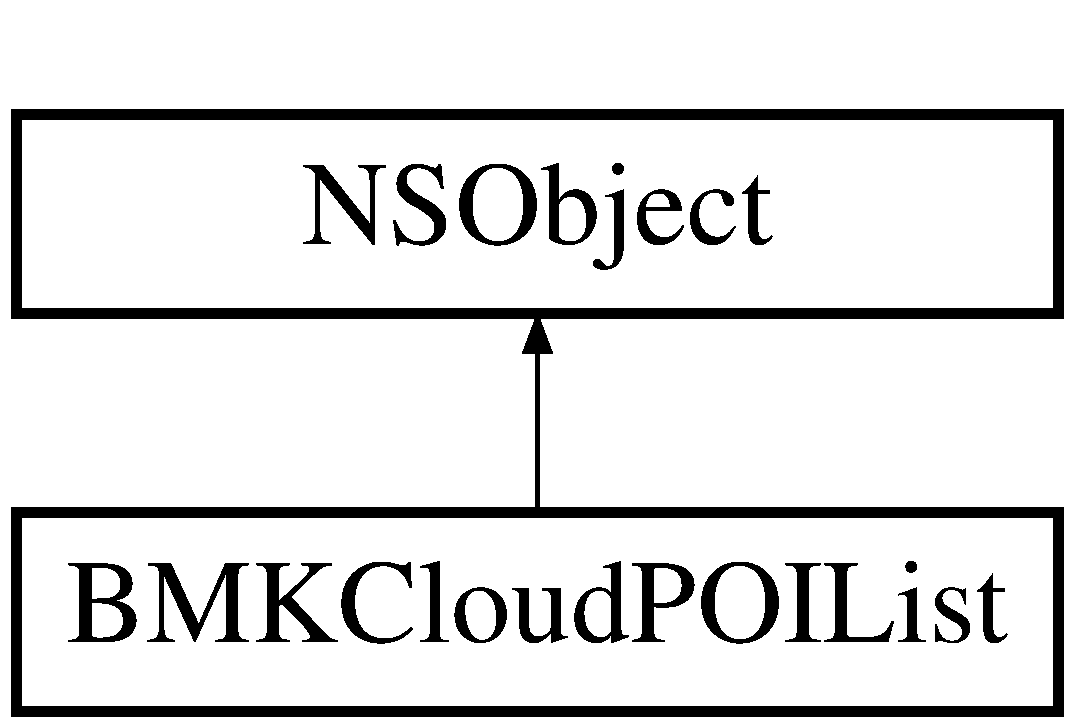
\includegraphics[height=2.000000cm]{interface_b_m_k_cloud_p_o_i_list}
\end{center}
\end{figure}
\subsection*{Protected 属性}
\begin{DoxyCompactItemize}
\item 
\hypertarget{interface_b_m_k_cloud_p_o_i_list_aeb5ee15bcbcfeaceb50cc735bcd5ca88}{N\+S\+Integer {\bfseries \+\_\+status}}\label{interface_b_m_k_cloud_p_o_i_list_aeb5ee15bcbcfeaceb50cc735bcd5ca88}

\item 
\hypertarget{interface_b_m_k_cloud_p_o_i_list_a0dead6846580429a7bca29d4c6336b90}{N\+S\+Integer {\bfseries \+\_\+total}}\label{interface_b_m_k_cloud_p_o_i_list_a0dead6846580429a7bca29d4c6336b90}

\item 
\hypertarget{interface_b_m_k_cloud_p_o_i_list_a43b86ee89f20f0bf99d10140fbc485ca}{N\+S\+Integer {\bfseries \+\_\+size}}\label{interface_b_m_k_cloud_p_o_i_list_a43b86ee89f20f0bf99d10140fbc485ca}

\item 
\hypertarget{interface_b_m_k_cloud_p_o_i_list_a1889b7fae8eef754ecac35daf15e65c6}{N\+S\+Integer {\bfseries \+\_\+page\+Num}}\label{interface_b_m_k_cloud_p_o_i_list_a1889b7fae8eef754ecac35daf15e65c6}

\item 
\hypertarget{interface_b_m_k_cloud_p_o_i_list_a513d425912e3517a7ae9286d8ef39d49}{N\+S\+Array $\ast$ {\bfseries \+\_\+\+P\+O\+Is}}\label{interface_b_m_k_cloud_p_o_i_list_a513d425912e3517a7ae9286d8ef39d49}

\end{DoxyCompactItemize}
\subsection*{属性}
\begin{DoxyCompactItemize}
\item 
\hypertarget{interface_b_m_k_cloud_p_o_i_list_a9a0761aa32216b6d96a3f3d538d8f2db}{N\+S\+Integer \hyperlink{interface_b_m_k_cloud_p_o_i_list_a9a0761aa32216b6d96a3f3d538d8f2db}{status}}\label{interface_b_m_k_cloud_p_o_i_list_a9a0761aa32216b6d96a3f3d538d8f2db}

\begin{DoxyCompactList}\small\item\em 搜索状态 \end{DoxyCompactList}\item 
\hypertarget{interface_b_m_k_cloud_p_o_i_list_a71aa046e96ad04026feb159383d3f615}{N\+S\+Integer \hyperlink{interface_b_m_k_cloud_p_o_i_list_a71aa046e96ad04026feb159383d3f615}{total}}\label{interface_b_m_k_cloud_p_o_i_list_a71aa046e96ad04026feb159383d3f615}

\begin{DoxyCompactList}\small\item\em 结果总数 \end{DoxyCompactList}\item 
\hypertarget{interface_b_m_k_cloud_p_o_i_list_a2d38d103dd34862c538ed99a635aafb5}{N\+S\+Integer \hyperlink{interface_b_m_k_cloud_p_o_i_list_a2d38d103dd34862c538ed99a635aafb5}{size}}\label{interface_b_m_k_cloud_p_o_i_list_a2d38d103dd34862c538ed99a635aafb5}

\begin{DoxyCompactList}\small\item\em 当前页返回数量 \end{DoxyCompactList}\item 
\hypertarget{interface_b_m_k_cloud_p_o_i_list_a1301275f0561c350c223dcf838502df8}{N\+S\+Integer \hyperlink{interface_b_m_k_cloud_p_o_i_list_a1301275f0561c350c223dcf838502df8}{page\+Num}}\label{interface_b_m_k_cloud_p_o_i_list_a1301275f0561c350c223dcf838502df8}

\begin{DoxyCompactList}\small\item\em 页数 \end{DoxyCompactList}\item 
\hypertarget{interface_b_m_k_cloud_p_o_i_list_a682ea5efc9695565e9ceacc9553d436d}{N\+S\+Array $\ast$ \hyperlink{interface_b_m_k_cloud_p_o_i_list_a682ea5efc9695565e9ceacc9553d436d}{P\+O\+Is}}\label{interface_b_m_k_cloud_p_o_i_list_a682ea5efc9695565e9ceacc9553d436d}

\begin{DoxyCompactList}\small\item\em P\+O\+I结果列表 \end{DoxyCompactList}\end{DoxyCompactItemize}


\subsection{详细描述}
云检索结果列表类 

该类的文档由以下文件生成\+:\begin{DoxyCompactItemize}
\item 
output/map\+\_\+search\+\_\+cloud\+\_\+loc\+\_\+util/inc/B\+M\+K\+Cloud\+P\+O\+I\+List.\+h\end{DoxyCompactItemize}

\hypertarget{interface_b_m_k_cloud_search}{\section{B\+M\+K\+Cloud\+Search类 参考}
\label{interface_b_m_k_cloud_search}\index{B\+M\+K\+Cloud\+Search@{B\+M\+K\+Cloud\+Search}}
}


云检索服务  




{\ttfamily \#import $<$B\+M\+K\+Cloud\+Search.\+h$>$}

类 B\+M\+K\+Cloud\+Search 继承关系图\+:\begin{figure}[H]
\begin{center}
\leavevmode
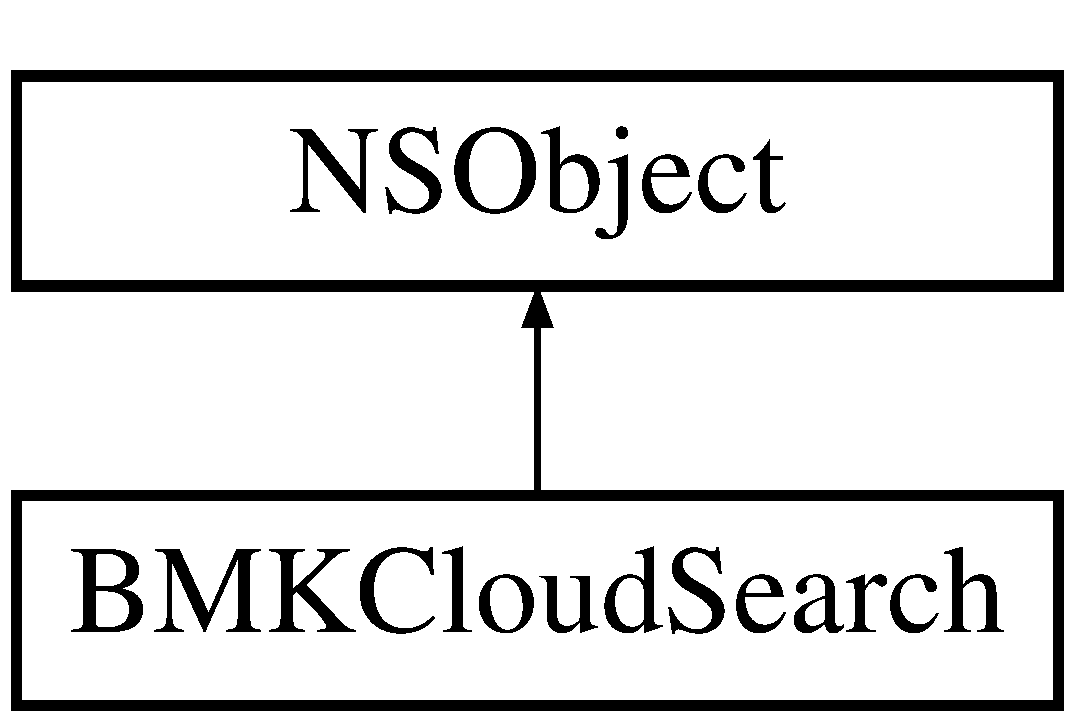
\includegraphics[height=2.000000cm]{interface_b_m_k_cloud_search}
\end{center}
\end{figure}
\subsection*{Instance Methods}
\begin{DoxyCompactItemize}
\item 
(B\+O\+O\+L) -\/ \hyperlink{interface_b_m_k_cloud_search_a473c4aeff275be5840ac6cf8010ce1d8}{local\+Search\+With\+Search\+Info\+:}
\item 
(B\+O\+O\+L) -\/ \hyperlink{interface_b_m_k_cloud_search_abe65e1b2f2b67e1d081c697caae80e4b}{nearby\+Search\+With\+Search\+Info\+:}
\item 
(B\+O\+O\+L) -\/ \hyperlink{interface_b_m_k_cloud_search_a7b2a5b409e884fb240e94f42cbad5208}{bound\+Search\+With\+Search\+Info\+:}
\item 
(B\+O\+O\+L) -\/ \hyperlink{interface_b_m_k_cloud_search_aaa7dcb1e49edd705290a3e79d8d22e92}{detail\+Search\+With\+Search\+Info\+:}
\end{DoxyCompactItemize}
\subsection*{属性}
\begin{DoxyCompactItemize}
\item 
\hypertarget{interface_b_m_k_cloud_search_ac35ac10ba735ab371814e2d69c27af23}{id$<$ \hyperlink{protocol_b_m_k_cloud_search_delegate-p}{B\+M\+K\+Cloud\+Search\+Delegate} $>$ \hyperlink{interface_b_m_k_cloud_search_ac35ac10ba735ab371814e2d69c27af23}{delegate}}\label{interface_b_m_k_cloud_search_ac35ac10ba735ab371814e2d69c27af23}

\begin{DoxyCompactList}\small\item\em 检索模块的\+Delegate,此处记得不用的时候需要置nil,否则影响内存的释放 \end{DoxyCompactList}\end{DoxyCompactItemize}


\subsection{详细描述}
云检索服务 

\subsection{Method Documentation}
\hypertarget{interface_b_m_k_cloud_search_a7b2a5b409e884fb240e94f42cbad5208}{\index{B\+M\+K\+Cloud\+Search@{B\+M\+K\+Cloud\+Search}!bound\+Search\+With\+Search\+Info\+:@{bound\+Search\+With\+Search\+Info\+:}}
\index{bound\+Search\+With\+Search\+Info\+:@{bound\+Search\+With\+Search\+Info\+:}!B\+M\+K\+Cloud\+Search@{B\+M\+K\+Cloud\+Search}}
\subsubsection[{bound\+Search\+With\+Search\+Info\+:}]{\setlength{\rightskip}{0pt plus 5cm}-\/ (B\+O\+O\+L) bound\+Search\+With\+Search\+Info\+: 
\begin{DoxyParamCaption}
\item[{({\bf B\+M\+K\+Cloud\+Bound\+Search\+Info} $\ast$)}]{search\+Info}
\end{DoxyParamCaption}
}}\label{interface_b_m_k_cloud_search_a7b2a5b409e884fb240e94f42cbad5208}
矩形云检索 异步函数,返回结果在\+B\+M\+K\+Cloud\+Search\+Delegate的on\+Get\+Cloud\+Poi\+Result通知 
\begin{DoxyParams}{参数}
{\em search\+Info} & 搜索参数 \\
\hline
\end{DoxyParams}
\begin{DoxyReturn}{返回}
成功返回\+Y\+E\+S,否则返回\+N\+O 
\end{DoxyReturn}
\hypertarget{interface_b_m_k_cloud_search_aaa7dcb1e49edd705290a3e79d8d22e92}{\index{B\+M\+K\+Cloud\+Search@{B\+M\+K\+Cloud\+Search}!detail\+Search\+With\+Search\+Info\+:@{detail\+Search\+With\+Search\+Info\+:}}
\index{detail\+Search\+With\+Search\+Info\+:@{detail\+Search\+With\+Search\+Info\+:}!B\+M\+K\+Cloud\+Search@{B\+M\+K\+Cloud\+Search}}
\subsubsection[{detail\+Search\+With\+Search\+Info\+:}]{\setlength{\rightskip}{0pt plus 5cm}-\/ (B\+O\+O\+L) detail\+Search\+With\+Search\+Info\+: 
\begin{DoxyParamCaption}
\item[{({\bf B\+M\+K\+Cloud\+Detail\+Search\+Info} $\ast$)}]{search\+Info}
\end{DoxyParamCaption}
}}\label{interface_b_m_k_cloud_search_aaa7dcb1e49edd705290a3e79d8d22e92}
详情云检索 异步函数,返回结果在\+B\+M\+K\+Cloud\+Search\+Delegate的on\+Get\+Cloud\+Poi\+Detail\+Result通知 
\begin{DoxyParams}{参数}
{\em search\+Info} & 搜索参数 \\
\hline
\end{DoxyParams}
\begin{DoxyReturn}{返回}
成功返回\+Y\+E\+S,否则返回\+N\+O 
\end{DoxyReturn}
\hypertarget{interface_b_m_k_cloud_search_a473c4aeff275be5840ac6cf8010ce1d8}{\index{B\+M\+K\+Cloud\+Search@{B\+M\+K\+Cloud\+Search}!local\+Search\+With\+Search\+Info\+:@{local\+Search\+With\+Search\+Info\+:}}
\index{local\+Search\+With\+Search\+Info\+:@{local\+Search\+With\+Search\+Info\+:}!B\+M\+K\+Cloud\+Search@{B\+M\+K\+Cloud\+Search}}
\subsubsection[{local\+Search\+With\+Search\+Info\+:}]{\setlength{\rightskip}{0pt plus 5cm}-\/ (B\+O\+O\+L) local\+Search\+With\+Search\+Info\+: 
\begin{DoxyParamCaption}
\item[{({\bf B\+M\+K\+Cloud\+Local\+Search\+Info} $\ast$)}]{search\+Info}
\end{DoxyParamCaption}
}}\label{interface_b_m_k_cloud_search_a473c4aeff275be5840ac6cf8010ce1d8}
本地云检索 异步函数,返回结果在\+B\+M\+K\+Cloud\+Search\+Delegate的on\+Get\+Cloud\+Poi\+Result通知 
\begin{DoxyParams}{参数}
{\em search\+Info} & 搜索参数 \\
\hline
\end{DoxyParams}
\begin{DoxyReturn}{返回}
成功返回\+Y\+E\+S,否则返回\+N\+O 
\end{DoxyReturn}
\hypertarget{interface_b_m_k_cloud_search_abe65e1b2f2b67e1d081c697caae80e4b}{\index{B\+M\+K\+Cloud\+Search@{B\+M\+K\+Cloud\+Search}!nearby\+Search\+With\+Search\+Info\+:@{nearby\+Search\+With\+Search\+Info\+:}}
\index{nearby\+Search\+With\+Search\+Info\+:@{nearby\+Search\+With\+Search\+Info\+:}!B\+M\+K\+Cloud\+Search@{B\+M\+K\+Cloud\+Search}}
\subsubsection[{nearby\+Search\+With\+Search\+Info\+:}]{\setlength{\rightskip}{0pt plus 5cm}-\/ (B\+O\+O\+L) nearby\+Search\+With\+Search\+Info\+: 
\begin{DoxyParamCaption}
\item[{({\bf B\+M\+K\+Cloud\+Nearby\+Search\+Info} $\ast$)}]{search\+Info}
\end{DoxyParamCaption}
}}\label{interface_b_m_k_cloud_search_abe65e1b2f2b67e1d081c697caae80e4b}
周边云检索 异步函数,返回结果在\+B\+M\+K\+Cloud\+Search\+Delegate的on\+Get\+Cloud\+Poi\+Result通知 
\begin{DoxyParams}{参数}
{\em search\+Info} & 搜索参数 \\
\hline
\end{DoxyParams}
\begin{DoxyReturn}{返回}
成功返回\+Y\+E\+S,否则返回\+N\+O 
\end{DoxyReturn}


该类的文档由以下文件生成\+:\begin{DoxyCompactItemize}
\item 
output/map\+\_\+search\+\_\+cloud\+\_\+loc\+\_\+util/inc/B\+M\+K\+Cloud\+Search.\+h\end{DoxyCompactItemize}

\hypertarget{protocol_b_m_k_cloud_search_delegate-p}{\section{$<$B\+M\+K\+Cloud\+Search\+Delegate$>$协议 参考}
\label{protocol_b_m_k_cloud_search_delegate-p}\index{$<$\+B\+M\+K\+Cloud\+Search\+Delegate$>$@{$<$\+B\+M\+K\+Cloud\+Search\+Delegate$>$}}
}


云检索delegate,用于获取云检索结果  




{\ttfamily \#import $<$B\+M\+K\+Cloud\+Search.\+h$>$}

类 $<$B\+M\+K\+Cloud\+Search\+Delegate$>$ 继承关系图\+:\begin{figure}[H]
\begin{center}
\leavevmode
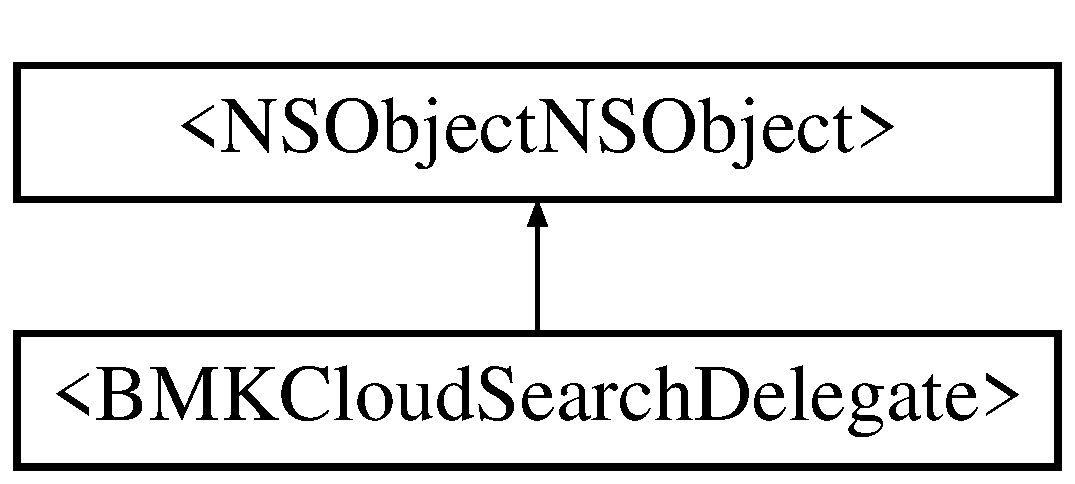
\includegraphics[height=2.000000cm]{protocol_b_m_k_cloud_search_delegate-p}
\end{center}
\end{figure}
\subsection*{Instance Methods}
\begin{DoxyCompactItemize}
\item 
(void) -\/ \hyperlink{protocol_b_m_k_cloud_search_delegate-p_aadc90dad37954d8527d4aca657c802f4}{on\+Get\+Cloud\+Poi\+Result\+:search\+Type\+:error\+Code\+:}
\item 
(void) -\/ \hyperlink{protocol_b_m_k_cloud_search_delegate-p_a5abcb777d4533baa036beb635268b60d}{on\+Get\+Cloud\+Poi\+Detail\+Result\+:search\+Type\+:error\+Code\+:}
\end{DoxyCompactItemize}


\subsection{详细描述}
云检索delegate,用于获取云检索结果 

\subsection{Method Documentation}
\hypertarget{protocol_b_m_k_cloud_search_delegate-p_a5abcb777d4533baa036beb635268b60d}{\index{B\+M\+K\+Cloud\+Search\+Delegate-\/p@{B\+M\+K\+Cloud\+Search\+Delegate-\/p}!on\+Get\+Cloud\+Poi\+Detail\+Result\+:search\+Type\+:error\+Code\+:@{on\+Get\+Cloud\+Poi\+Detail\+Result\+:search\+Type\+:error\+Code\+:}}
\index{on\+Get\+Cloud\+Poi\+Detail\+Result\+:search\+Type\+:error\+Code\+:@{on\+Get\+Cloud\+Poi\+Detail\+Result\+:search\+Type\+:error\+Code\+:}!B\+M\+K\+Cloud\+Search\+Delegate-\/p@{B\+M\+K\+Cloud\+Search\+Delegate-\/p}}
\subsubsection[{on\+Get\+Cloud\+Poi\+Detail\+Result\+:search\+Type\+:error\+Code\+:}]{\setlength{\rightskip}{0pt plus 5cm}-\/ (void) on\+Get\+Cloud\+Poi\+Detail\+Result\+: 
\begin{DoxyParamCaption}
\item[{({\bf B\+M\+K\+Cloud\+P\+O\+I\+Info} $\ast$)}]{poi\+Detail\+Result}
\item[{searchType:(int)}]{type}
\item[{errorCode:(int)}]{error}
\end{DoxyParamCaption}
\hspace{0.3cm}{\ttfamily [optional]}}}\label{protocol_b_m_k_cloud_search_delegate-p_a5abcb777d4533baa036beb635268b60d}
返回云检索\+P\+O\+I详情 
\begin{DoxyParams}{参数}
{\em poi\+Detail\+Result} & 类型为\+B\+M\+K\+Cloud\+P\+O\+I\+Info \\
\hline
{\em type} & 返回结果类型: B\+M\+K\+\_\+\+C\+L\+O\+U\+D\+\_\+\+D\+E\+T\+A\+I\+L\+\_\+\+S\+E\+A\+R\+C\+H \\
\hline
{\em error} & 错误号,\\
\hline
\end{DoxyParams}
\begin{DoxySeeAlso}{参见}
B\+M\+K\+Error\+Code 
\end{DoxySeeAlso}
\hypertarget{protocol_b_m_k_cloud_search_delegate-p_aadc90dad37954d8527d4aca657c802f4}{\index{B\+M\+K\+Cloud\+Search\+Delegate-\/p@{B\+M\+K\+Cloud\+Search\+Delegate-\/p}!on\+Get\+Cloud\+Poi\+Result\+:search\+Type\+:error\+Code\+:@{on\+Get\+Cloud\+Poi\+Result\+:search\+Type\+:error\+Code\+:}}
\index{on\+Get\+Cloud\+Poi\+Result\+:search\+Type\+:error\+Code\+:@{on\+Get\+Cloud\+Poi\+Result\+:search\+Type\+:error\+Code\+:}!B\+M\+K\+Cloud\+Search\+Delegate-\/p@{B\+M\+K\+Cloud\+Search\+Delegate-\/p}}
\subsubsection[{on\+Get\+Cloud\+Poi\+Result\+:search\+Type\+:error\+Code\+:}]{\setlength{\rightskip}{0pt plus 5cm}-\/ (void) on\+Get\+Cloud\+Poi\+Result\+: 
\begin{DoxyParamCaption}
\item[{(N\+S\+Array $\ast$)}]{poi\+Result\+List}
\item[{searchType:(int)}]{type}
\item[{errorCode:(int)}]{error}
\end{DoxyParamCaption}
\hspace{0.3cm}{\ttfamily [optional]}}}\label{protocol_b_m_k_cloud_search_delegate-p_aadc90dad37954d8527d4aca657c802f4}
返回云检索\+P\+O\+I列表结果 
\begin{DoxyParams}{参数}
{\em poi\+Result\+List} & 云检索结果列表,成员类型为\+B\+M\+K\+Cloud\+P\+O\+I\+List \\
\hline
{\em type} & 返回结果类型: B\+M\+K\+\_\+\+C\+L\+O\+U\+D\+\_\+\+L\+O\+C\+A\+L\+\_\+\+S\+E\+A\+R\+C\+H,B\+M\+K\+\_\+\+C\+L\+O\+U\+D\+\_\+\+N\+E\+A\+R\+B\+Y\+\_\+\+S\+E\+A\+R\+C\+H,B\+M\+K\+\_\+\+C\+L\+O\+U\+D\+\_\+\+B\+O\+U\+N\+D\+\_\+\+S\+E\+A\+R\+C\+H \\
\hline
{\em error} & 错误号,\\
\hline
\end{DoxyParams}
\begin{DoxySeeAlso}{参见}
B\+M\+K\+Error\+Code 
\end{DoxySeeAlso}


该协议的文档由以下文件生成\+:\begin{DoxyCompactItemize}
\item 
output/map\+\_\+search\+\_\+cloud\+\_\+loc\+\_\+util/inc/B\+M\+K\+Cloud\+Search.\+h\end{DoxyCompactItemize}

\hypertarget{interface_b_m_k_cloud_search_info}{\section{B\+M\+K\+Cloud\+Search\+Info类 参考}
\label{interface_b_m_k_cloud_search_info}\index{B\+M\+K\+Cloud\+Search\+Info@{B\+M\+K\+Cloud\+Search\+Info}}
}


本地,周边,矩形云检索基础信息类  




{\ttfamily \#import $<$B\+M\+K\+Cloud\+Search\+Info.\+h$>$}

类 B\+M\+K\+Cloud\+Search\+Info 继承关系图\+:\begin{figure}[H]
\begin{center}
\leavevmode
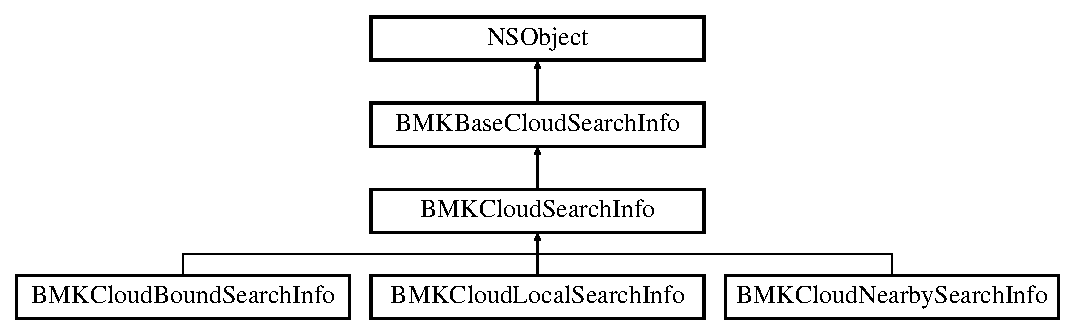
\includegraphics[height=4.000000cm]{interface_b_m_k_cloud_search_info}
\end{center}
\end{figure}
\subsection*{Protected 属性}
\begin{DoxyCompactItemize}
\item 
\hypertarget{interface_b_m_k_cloud_search_info_a5422fe46667de549c2b294ceb921a78b}{N\+S\+String $\ast$ {\bfseries \+\_\+keyword}}\label{interface_b_m_k_cloud_search_info_a5422fe46667de549c2b294ceb921a78b}

\item 
\hypertarget{interface_b_m_k_cloud_search_info_a40b12c1fbccf0956451838cd83f82be0}{N\+S\+String $\ast$ {\bfseries \+\_\+tags}}\label{interface_b_m_k_cloud_search_info_a40b12c1fbccf0956451838cd83f82be0}

\item 
\hypertarget{interface_b_m_k_cloud_search_info_a263c562ad6526d87421ec56a7ea55ea0}{N\+S\+String $\ast$ {\bfseries \+\_\+sortby}}\label{interface_b_m_k_cloud_search_info_a263c562ad6526d87421ec56a7ea55ea0}

\item 
\hypertarget{interface_b_m_k_cloud_search_info_a03b41d160bf2aaec634b34296dc5f0c5}{N\+S\+String $\ast$ {\bfseries \+\_\+filter}}\label{interface_b_m_k_cloud_search_info_a03b41d160bf2aaec634b34296dc5f0c5}

\item 
\hypertarget{interface_b_m_k_cloud_search_info_ac0e87c49e04dc123eb147ff4bf1e8cb6}{N\+S\+Integer {\bfseries \+\_\+page\+Index}}\label{interface_b_m_k_cloud_search_info_ac0e87c49e04dc123eb147ff4bf1e8cb6}

\item 
\hypertarget{interface_b_m_k_cloud_search_info_aca814c9ad2df72058f20575244e64ec3}{N\+S\+Integer {\bfseries \+\_\+page\+Size}}\label{interface_b_m_k_cloud_search_info_aca814c9ad2df72058f20575244e64ec3}

\end{DoxyCompactItemize}
\subsection*{属性}
\begin{DoxyCompactItemize}
\item 
\hypertarget{interface_b_m_k_cloud_search_info_a90f2d3ef36a31112ca8fdb6d70fabea6}{N\+S\+String $\ast$ \hyperlink{interface_b_m_k_cloud_search_info_a90f2d3ef36a31112ca8fdb6d70fabea6}{keyword}}\label{interface_b_m_k_cloud_search_info_a90f2d3ef36a31112ca8fdb6d70fabea6}

\begin{DoxyCompactList}\small\item\em 检索关键字,必选。最长45个字符 \end{DoxyCompactList}\item 
\hypertarget{interface_b_m_k_cloud_search_info_ae2c16f1281195d1fbf738ac23552d8f7}{N\+S\+String $\ast$ \hyperlink{interface_b_m_k_cloud_search_info_ae2c16f1281195d1fbf738ac23552d8f7}{tags}}\label{interface_b_m_k_cloud_search_info_ae2c16f1281195d1fbf738ac23552d8f7}

\begin{DoxyCompactList}\small\item\em 标签,可选,空格分隔的多字符串,最长45个字符,样例:美食 小吃 \end{DoxyCompactList}\item 
N\+S\+String $\ast$ \hyperlink{interface_b_m_k_cloud_search_info_ab0d42d1b9e841c5e538e457e819a07f7}{sortby}
\begin{DoxyCompactList}\small\item\em 排序字段,可选: sortby=\{keyname\}\+:1 升序;sortby=\{keyname\}\+:-\/1 降序 \end{DoxyCompactList}\item 
N\+S\+String $\ast$ \hyperlink{interface_b_m_k_cloud_search_info_a65d91501d19f2a6aa027de6f9e5bc837}{filter}
\begin{DoxyCompactList}\small\item\em 过滤条件,可选\+:'$\vert$'竖线分隔的多个key-\/value对,price\+:9.\+99,19.\+99$\vert$time\+:2012,2012 \end{DoxyCompactList}\item 
\hypertarget{interface_b_m_k_cloud_search_info_aeea99c3907cafe38def8105839ad4c8a}{N\+S\+Integer \hyperlink{interface_b_m_k_cloud_search_info_aeea99c3907cafe38def8105839ad4c8a}{page\+Index}}\label{interface_b_m_k_cloud_search_info_aeea99c3907cafe38def8105839ad4c8a}

\begin{DoxyCompactList}\small\item\em 分页索引,可选,默认为0 \end{DoxyCompactList}\item 
\hypertarget{interface_b_m_k_cloud_search_info_ab625992f8620205a6b24a1490a999fde}{N\+S\+Integer \hyperlink{interface_b_m_k_cloud_search_info_ab625992f8620205a6b24a1490a999fde}{page\+Size}}\label{interface_b_m_k_cloud_search_info_ab625992f8620205a6b24a1490a999fde}

\begin{DoxyCompactList}\small\item\em 分页数量,可选,默认为10,最多为50 \end{DoxyCompactList}\end{DoxyCompactItemize}


\subsection{详细描述}
本地,周边,矩形云检索基础信息类 

\subsection{属性说明}
\hypertarget{interface_b_m_k_cloud_search_info_a65d91501d19f2a6aa027de6f9e5bc837}{\index{B\+M\+K\+Cloud\+Search\+Info@{B\+M\+K\+Cloud\+Search\+Info}!filter@{filter}}
\index{filter@{filter}!B\+M\+K\+Cloud\+Search\+Info@{B\+M\+K\+Cloud\+Search\+Info}}
\subsubsection[{filter}]{\setlength{\rightskip}{0pt plus 5cm}-\/ (N\+S\+String$\ast$) filter\hspace{0.3cm}{\ttfamily [read]}, {\ttfamily [write]}, {\ttfamily [nonatomic]}, {\ttfamily [strong]}}}\label{interface_b_m_k_cloud_search_info_a65d91501d19f2a6aa027de6f9e5bc837}


过滤条件,可选\+:'$\vert$'竖线分隔的多个key-\/value对,price\+:9.\+99,19.\+99$\vert$time\+:2012,2012 

过滤条件,可选 '$\vert$'竖线分隔的多个key-\/value对 key为筛选字段的名称(存储服务中定义) value可以是整形或者浮点数的一个区间:格式为“small,big”逗号分隔的2个数字 样例:筛选价格为9.99到19.99并且生产时间为2013年的项:price\+:9.\+99,19.\+99$\vert$time\+:2012,2012 \hypertarget{interface_b_m_k_cloud_search_info_ab0d42d1b9e841c5e538e457e819a07f7}{\index{B\+M\+K\+Cloud\+Search\+Info@{B\+M\+K\+Cloud\+Search\+Info}!sortby@{sortby}}
\index{sortby@{sortby}!B\+M\+K\+Cloud\+Search\+Info@{B\+M\+K\+Cloud\+Search\+Info}}
\subsubsection[{sortby}]{\setlength{\rightskip}{0pt plus 5cm}-\/ (N\+S\+String$\ast$) sortby\hspace{0.3cm}{\ttfamily [read]}, {\ttfamily [write]}, {\ttfamily [nonatomic]}, {\ttfamily [strong]}}}\label{interface_b_m_k_cloud_search_info_ab0d42d1b9e841c5e538e457e819a07f7}


排序字段,可选: sortby=\{keyname\}\+:1 升序;sortby=\{keyname\}\+:-\/1 降序 

排序字段,可选: sortby=\{keyname\}\+:1 升序;sortby=\{keyname\}\+:-\/1 降序。 以下keyname为系统预定义的: 1.\+distance 距离排序 2.\+weight 权重排序 默认为按weight排序 如果需要自定义排序则指定排序字段 样例:按照价格由便宜到贵排序sortby=price\+:1 

该类的文档由以下文件生成\+:\begin{DoxyCompactItemize}
\item 
output/map\+\_\+search\+\_\+cloud\+\_\+loc\+\_\+util/inc/B\+M\+K\+Cloud\+Search\+Info.\+h\end{DoxyCompactItemize}

\hypertarget{struct_b_m_k_coordinate_bounds}{\section{B\+M\+K\+Coordinate\+Bounds结构体 参考}
\label{struct_b_m_k_coordinate_bounds}\index{B\+M\+K\+Coordinate\+Bounds@{B\+M\+K\+Coordinate\+Bounds}}
}


表示一个经纬度区域  




{\ttfamily \#include $<$B\+M\+K\+Types.\+h$>$}

\subsection*{Public 属性}
\begin{DoxyCompactItemize}
\item 
\hypertarget{struct_b_m_k_coordinate_bounds_a0ebf42cb8682f2a6990fc7c6e439702e}{C\+L\+Location\+Coordinate2\+D \hyperlink{struct_b_m_k_coordinate_bounds_a0ebf42cb8682f2a6990fc7c6e439702e}{north\+East}}\label{struct_b_m_k_coordinate_bounds_a0ebf42cb8682f2a6990fc7c6e439702e}

\begin{DoxyCompactList}\small\item\em 东北角点经纬度坐标 \end{DoxyCompactList}\item 
\hypertarget{struct_b_m_k_coordinate_bounds_afd02c24b2ffe5aba18a125a48cdd1c37}{C\+L\+Location\+Coordinate2\+D \hyperlink{struct_b_m_k_coordinate_bounds_afd02c24b2ffe5aba18a125a48cdd1c37}{south\+West}}\label{struct_b_m_k_coordinate_bounds_afd02c24b2ffe5aba18a125a48cdd1c37}

\begin{DoxyCompactList}\small\item\em 西南角点经纬度坐标 \end{DoxyCompactList}\end{DoxyCompactItemize}


\subsection{详细描述}
表示一个经纬度区域 

该结构体的文档由以下文件生成\+:\begin{DoxyCompactItemize}
\item 
output/map\+\_\+search\+\_\+cloud\+\_\+loc\+\_\+util/inc/B\+M\+K\+Types.\+h\end{DoxyCompactItemize}

\hypertarget{struct_b_m_k_coordinate_region}{\section{B\+M\+K\+Coordinate\+Region结构体 参考}
\label{struct_b_m_k_coordinate_region}\index{B\+M\+K\+Coordinate\+Region@{B\+M\+K\+Coordinate\+Region}}
}


表示一个经纬度区域  




{\ttfamily \#include $<$B\+M\+K\+Types.\+h$>$}

\subsection*{Public 属性}
\begin{DoxyCompactItemize}
\item 
\hypertarget{struct_b_m_k_coordinate_region_a298c069df033a5690fdebc3c63f86903}{C\+L\+Location\+Coordinate2\+D \hyperlink{struct_b_m_k_coordinate_region_a298c069df033a5690fdebc3c63f86903}{center}}\label{struct_b_m_k_coordinate_region_a298c069df033a5690fdebc3c63f86903}

\begin{DoxyCompactList}\small\item\em 中心点经纬度坐标 \end{DoxyCompactList}\item 
\hypertarget{struct_b_m_k_coordinate_region_a75e65758cbbf7cb3ed6007d4ce301292}{\hyperlink{struct_b_m_k_coordinate_span}{B\+M\+K\+Coordinate\+Span} \hyperlink{struct_b_m_k_coordinate_region_a75e65758cbbf7cb3ed6007d4ce301292}{span}}\label{struct_b_m_k_coordinate_region_a75e65758cbbf7cb3ed6007d4ce301292}

\begin{DoxyCompactList}\small\item\em 经纬度范围 \end{DoxyCompactList}\end{DoxyCompactItemize}


\subsection{详细描述}
表示一个经纬度区域 

该结构体的文档由以下文件生成\+:\begin{DoxyCompactItemize}
\item 
output/map\+\_\+search\+\_\+cloud\+\_\+loc\+\_\+util/inc/B\+M\+K\+Types.\+h\end{DoxyCompactItemize}

\hypertarget{struct_b_m_k_coordinate_span}{\section{B\+M\+K\+Coordinate\+Span结构体 参考}
\label{struct_b_m_k_coordinate_span}\index{B\+M\+K\+Coordinate\+Span@{B\+M\+K\+Coordinate\+Span}}
}


表示一个经纬度范围  




{\ttfamily \#include $<$B\+M\+K\+Types.\+h$>$}

\subsection*{Public 属性}
\begin{DoxyCompactItemize}
\item 
\hypertarget{struct_b_m_k_coordinate_span_a759543f626366ce4fe599b8896f352a2}{C\+L\+Location\+Degrees \hyperlink{struct_b_m_k_coordinate_span_a759543f626366ce4fe599b8896f352a2}{latitude\+Delta}}\label{struct_b_m_k_coordinate_span_a759543f626366ce4fe599b8896f352a2}

\begin{DoxyCompactList}\small\item\em 纬度范围 \end{DoxyCompactList}\item 
\hypertarget{struct_b_m_k_coordinate_span_ab3bc7d18bbd0fce7c806c51f0e0df447}{C\+L\+Location\+Degrees \hyperlink{struct_b_m_k_coordinate_span_ab3bc7d18bbd0fce7c806c51f0e0df447}{longitude\+Delta}}\label{struct_b_m_k_coordinate_span_ab3bc7d18bbd0fce7c806c51f0e0df447}

\begin{DoxyCompactList}\small\item\em 经度范围 \end{DoxyCompactList}\end{DoxyCompactItemize}


\subsection{详细描述}
表示一个经纬度范围 

该结构体的文档由以下文件生成\+:\begin{DoxyCompactItemize}
\item 
output/map\+\_\+search\+\_\+cloud\+\_\+loc\+\_\+util/inc/B\+M\+K\+Types.\+h\end{DoxyCompactItemize}

\hypertarget{interface_b_m_k_driving_route_line}{\section{B\+M\+K\+Driving\+Route\+Line类 参考}
\label{interface_b_m_k_driving_route_line}\index{B\+M\+K\+Driving\+Route\+Line@{B\+M\+K\+Driving\+Route\+Line}}
}


此类表示一条驾车路线  




{\ttfamily \#import $<$B\+M\+K\+Route\+Search\+Type.\+h$>$}

类 B\+M\+K\+Driving\+Route\+Line 继承关系图\+:\begin{figure}[H]
\begin{center}
\leavevmode
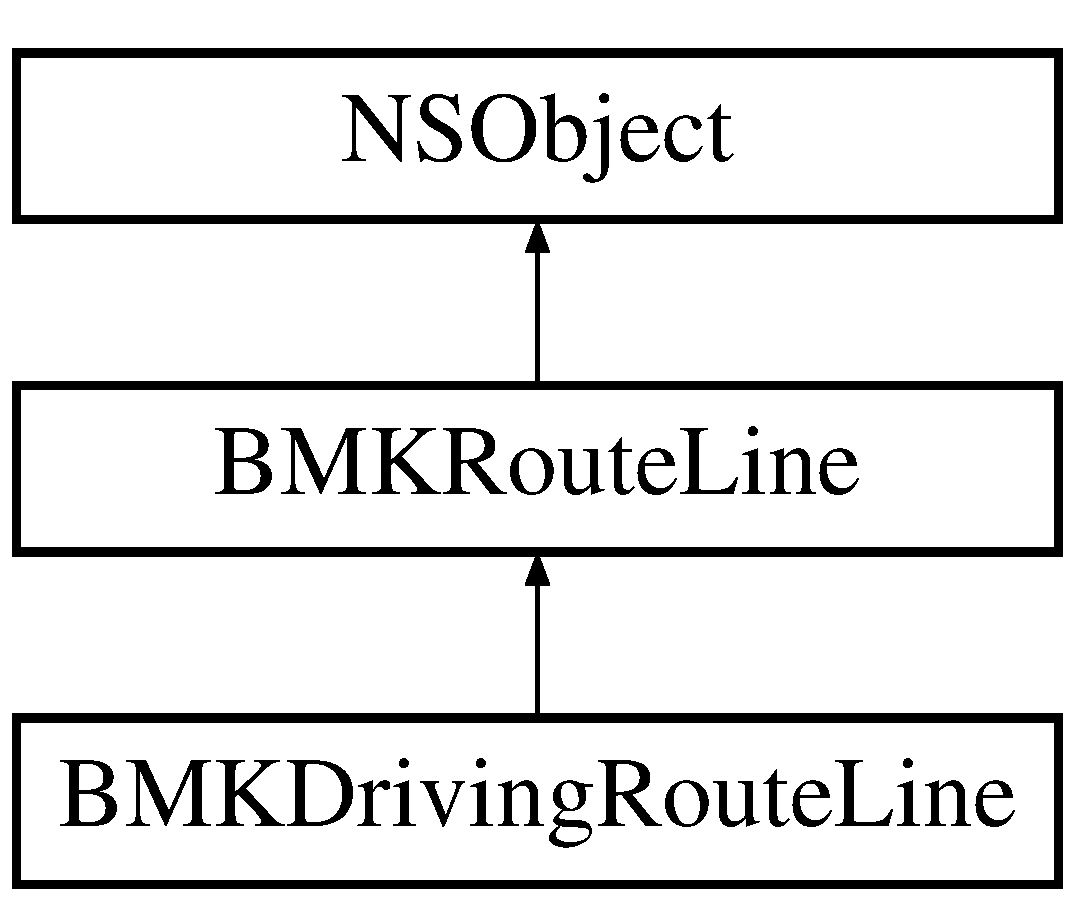
\includegraphics[height=3.000000cm]{interface_b_m_k_driving_route_line}
\end{center}
\end{figure}
\subsection*{Protected 属性}
\begin{DoxyCompactItemize}
\item 
\hypertarget{interface_b_m_k_driving_route_line_ac5d75fa8fdd883982c7870e821b93da0}{bool {\bfseries \+\_\+is\+Support\+Traffic}}\label{interface_b_m_k_driving_route_line_ac5d75fa8fdd883982c7870e821b93da0}

\item 
\hypertarget{interface_b_m_k_driving_route_line_a371d37ca24cff8e33b6f1540fdbab3a4}{N\+S\+Array $\ast$ {\bfseries \+\_\+way\+Points}}\label{interface_b_m_k_driving_route_line_a371d37ca24cff8e33b6f1540fdbab3a4}

\end{DoxyCompactItemize}
\subsection*{属性}
\begin{DoxyCompactItemize}
\item 
\hypertarget{interface_b_m_k_driving_route_line_a23c30bf764fd27531e7f7d1e1cb1d6b4}{bool \hyperlink{interface_b_m_k_driving_route_line_a23c30bf764fd27531e7f7d1e1cb1d6b4}{is\+Support\+Traffic}}\label{interface_b_m_k_driving_route_line_a23c30bf764fd27531e7f7d1e1cb1d6b4}

\begin{DoxyCompactList}\small\item\em 该路线所在区域是否含有交通流量信息 \end{DoxyCompactList}\item 
\hypertarget{interface_b_m_k_driving_route_line_a577c5a10368ef9c18ac73f20836092bd}{N\+S\+Array $\ast$ \hyperlink{interface_b_m_k_driving_route_line_a577c5a10368ef9c18ac73f20836092bd}{way\+Points}}\label{interface_b_m_k_driving_route_line_a577c5a10368ef9c18ac73f20836092bd}

\begin{DoxyCompactList}\small\item\em 路线途经点列表,成员类型为\+B\+M\+K\+Plan\+Node \end{DoxyCompactList}\end{DoxyCompactItemize}


\subsection{详细描述}
此类表示一条驾车路线 

该类的文档由以下文件生成\+:\begin{DoxyCompactItemize}
\item 
output/map\+\_\+search\+\_\+cloud\+\_\+loc\+\_\+util/inc/B\+M\+K\+Route\+Search\+Type.\+h\end{DoxyCompactItemize}

\hypertarget{interface_b_m_k_driving_route_plan_option}{\section{B\+M\+K\+Driving\+Route\+Plan\+Option类 参考}
\label{interface_b_m_k_driving_route_plan_option}\index{B\+M\+K\+Driving\+Route\+Plan\+Option@{B\+M\+K\+Driving\+Route\+Plan\+Option}}
}


驾车查询基础信息类  




{\ttfamily \#import $<$B\+M\+K\+Route\+Search\+Option.\+h$>$}

类 B\+M\+K\+Driving\+Route\+Plan\+Option 继承关系图\+:\begin{figure}[H]
\begin{center}
\leavevmode
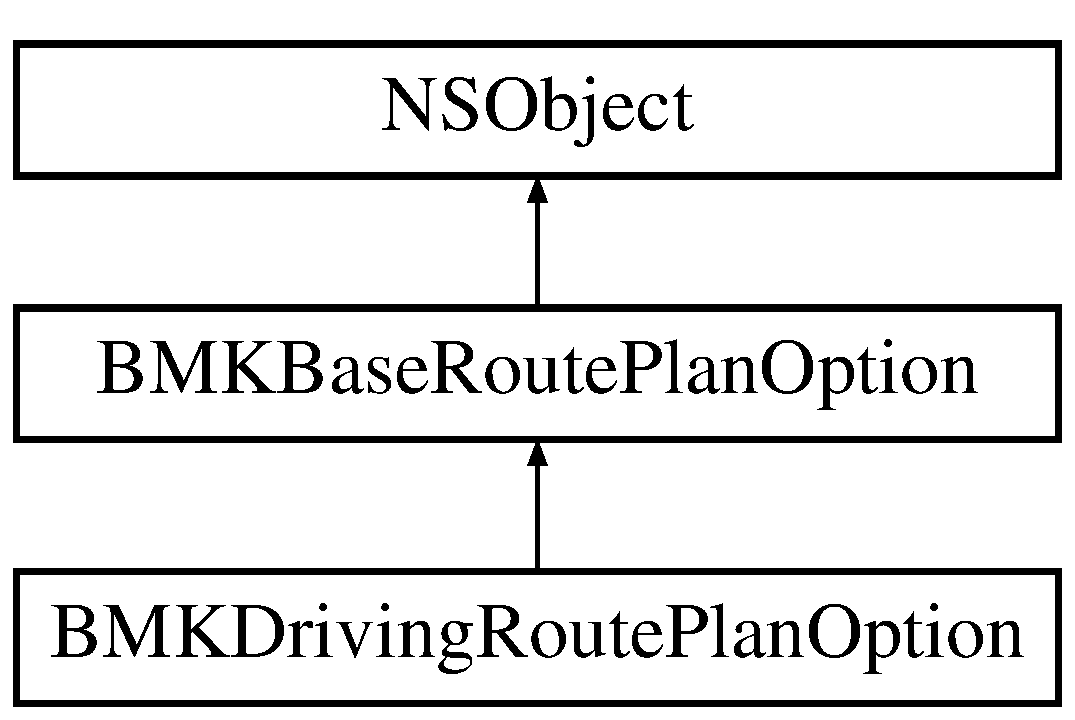
\includegraphics[height=3.000000cm]{interface_b_m_k_driving_route_plan_option}
\end{center}
\end{figure}
\subsection*{Protected 属性}
\begin{DoxyCompactItemize}
\item 
\hypertarget{interface_b_m_k_driving_route_plan_option_aac7dd49a6a8f7133ff8207b59bbb03ab}{N\+S\+Array $\ast$ {\bfseries \+\_\+way\+Points\+Array}}\label{interface_b_m_k_driving_route_plan_option_aac7dd49a6a8f7133ff8207b59bbb03ab}

\item 
\hypertarget{interface_b_m_k_driving_route_plan_option_a6378c481740e1aff326001bff3c28738}{B\+M\+K\+Driving\+Policy {\bfseries \+\_\+driving\+Policy}}\label{interface_b_m_k_driving_route_plan_option_a6378c481740e1aff326001bff3c28738}

\end{DoxyCompactItemize}
\subsection*{属性}
\begin{DoxyCompactItemize}
\item 
\hypertarget{interface_b_m_k_driving_route_plan_option_a13b365a390f0ccfc2f2b5d16927eb9db}{N\+S\+Array $\ast$ {\bfseries way\+Points\+Array}}\label{interface_b_m_k_driving_route_plan_option_a13b365a390f0ccfc2f2b5d16927eb9db}

\item 
\hypertarget{interface_b_m_k_driving_route_plan_option_a51fe8957c72c8d0d478515bd7afa0cfd}{B\+M\+K\+Driving\+Policy \hyperlink{interface_b_m_k_driving_route_plan_option_a51fe8957c72c8d0d478515bd7afa0cfd}{driving\+Policy}}\label{interface_b_m_k_driving_route_plan_option_a51fe8957c72c8d0d478515bd7afa0cfd}

\begin{DoxyCompactList}\small\item\em 驾车检索策略 \end{DoxyCompactList}\end{DoxyCompactItemize}


\subsection{详细描述}
驾车查询基础信息类 

该类的文档由以下文件生成\+:\begin{DoxyCompactItemize}
\item 
output/map\+\_\+search\+\_\+cloud\+\_\+loc\+\_\+util/inc/B\+M\+K\+Route\+Search\+Option.\+h\end{DoxyCompactItemize}

\hypertarget{interface_b_m_k_driving_route_result}{\section{B\+M\+K\+Driving\+Route\+Result类 参考}
\label{interface_b_m_k_driving_route_result}\index{B\+M\+K\+Driving\+Route\+Result@{B\+M\+K\+Driving\+Route\+Result}}
}


此类表示驾车路线结果  




{\ttfamily \#import $<$B\+M\+K\+Route\+Search\+Type.\+h$>$}

类 B\+M\+K\+Driving\+Route\+Result 继承关系图\+:\begin{figure}[H]
\begin{center}
\leavevmode
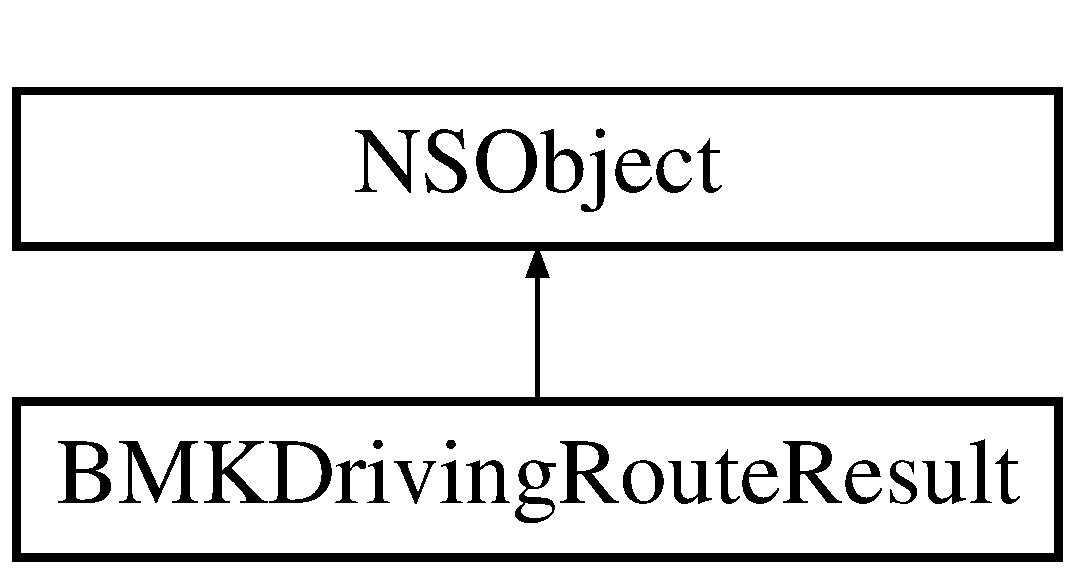
\includegraphics[height=2.000000cm]{interface_b_m_k_driving_route_result}
\end{center}
\end{figure}
\subsection*{Protected 属性}
\begin{DoxyCompactItemize}
\item 
\hypertarget{interface_b_m_k_driving_route_result_ad4dfb5abdc9df74cda947b4796879a13}{\hyperlink{interface_b_m_k_taxi_info}{B\+M\+K\+Taxi\+Info} $\ast$ {\bfseries \+\_\+taxi\+Info}}\label{interface_b_m_k_driving_route_result_ad4dfb5abdc9df74cda947b4796879a13}

\item 
\hypertarget{interface_b_m_k_driving_route_result_a7401197c1f543949165707362be5fcbb}{\hyperlink{interface_b_m_k_suggest_addr_info}{B\+M\+K\+Suggest\+Addr\+Info} $\ast$ {\bfseries \+\_\+suggest\+Addr\+Result}}\label{interface_b_m_k_driving_route_result_a7401197c1f543949165707362be5fcbb}

\item 
\hypertarget{interface_b_m_k_driving_route_result_a3a5b54ae9219585248392bbeaa5d9c42}{N\+S\+Array $\ast$ {\bfseries \+\_\+routes}}\label{interface_b_m_k_driving_route_result_a3a5b54ae9219585248392bbeaa5d9c42}

\end{DoxyCompactItemize}
\subsection*{属性}
\begin{DoxyCompactItemize}
\item 
\hypertarget{interface_b_m_k_driving_route_result_a4dc537f67ed47de78ac3bcda172397dd}{\hyperlink{interface_b_m_k_taxi_info}{B\+M\+K\+Taxi\+Info} $\ast$ \hyperlink{interface_b_m_k_driving_route_result_a4dc537f67ed47de78ac3bcda172397dd}{taxi\+Info}}\label{interface_b_m_k_driving_route_result_a4dc537f67ed47de78ac3bcda172397dd}

\begin{DoxyCompactList}\small\item\em 该路线打车信息 \end{DoxyCompactList}\item 
\hypertarget{interface_b_m_k_driving_route_result_adf554437aec4884ae9fdc7cdb8fc2625}{\hyperlink{interface_b_m_k_suggest_addr_info}{B\+M\+K\+Suggest\+Addr\+Info} $\ast$ \hyperlink{interface_b_m_k_driving_route_result_adf554437aec4884ae9fdc7cdb8fc2625}{suggest\+Addr\+Result}}\label{interface_b_m_k_driving_route_result_adf554437aec4884ae9fdc7cdb8fc2625}

\begin{DoxyCompactList}\small\item\em 返回起点或终点的地址信息结果 \end{DoxyCompactList}\item 
\hypertarget{interface_b_m_k_driving_route_result_a448147e99f71f6bf82c93a51dd2d4b81}{N\+S\+Array $\ast$ \hyperlink{interface_b_m_k_driving_route_result_a448147e99f71f6bf82c93a51dd2d4b81}{routes}}\label{interface_b_m_k_driving_route_result_a448147e99f71f6bf82c93a51dd2d4b81}

\begin{DoxyCompactList}\small\item\em 驾车结果,现在只返回一条。成员类型为\+B\+M\+K\+Driving\+Route\+Line \end{DoxyCompactList}\end{DoxyCompactItemize}


\subsection{详细描述}
此类表示驾车路线结果 

该类的文档由以下文件生成\+:\begin{DoxyCompactItemize}
\item 
output/map\+\_\+search\+\_\+cloud\+\_\+loc\+\_\+util/inc/B\+M\+K\+Route\+Search\+Type.\+h\end{DoxyCompactItemize}

\hypertarget{interface_b_m_k_driving_step}{\section{B\+M\+K\+Driving\+Step类 参考}
\label{interface_b_m_k_driving_step}\index{B\+M\+K\+Driving\+Step@{B\+M\+K\+Driving\+Step}}
}


此类表示驾车路线中的一个路段  




{\ttfamily \#import $<$B\+M\+K\+Route\+Search\+Type.\+h$>$}

类 B\+M\+K\+Driving\+Step 继承关系图\+:\begin{figure}[H]
\begin{center}
\leavevmode
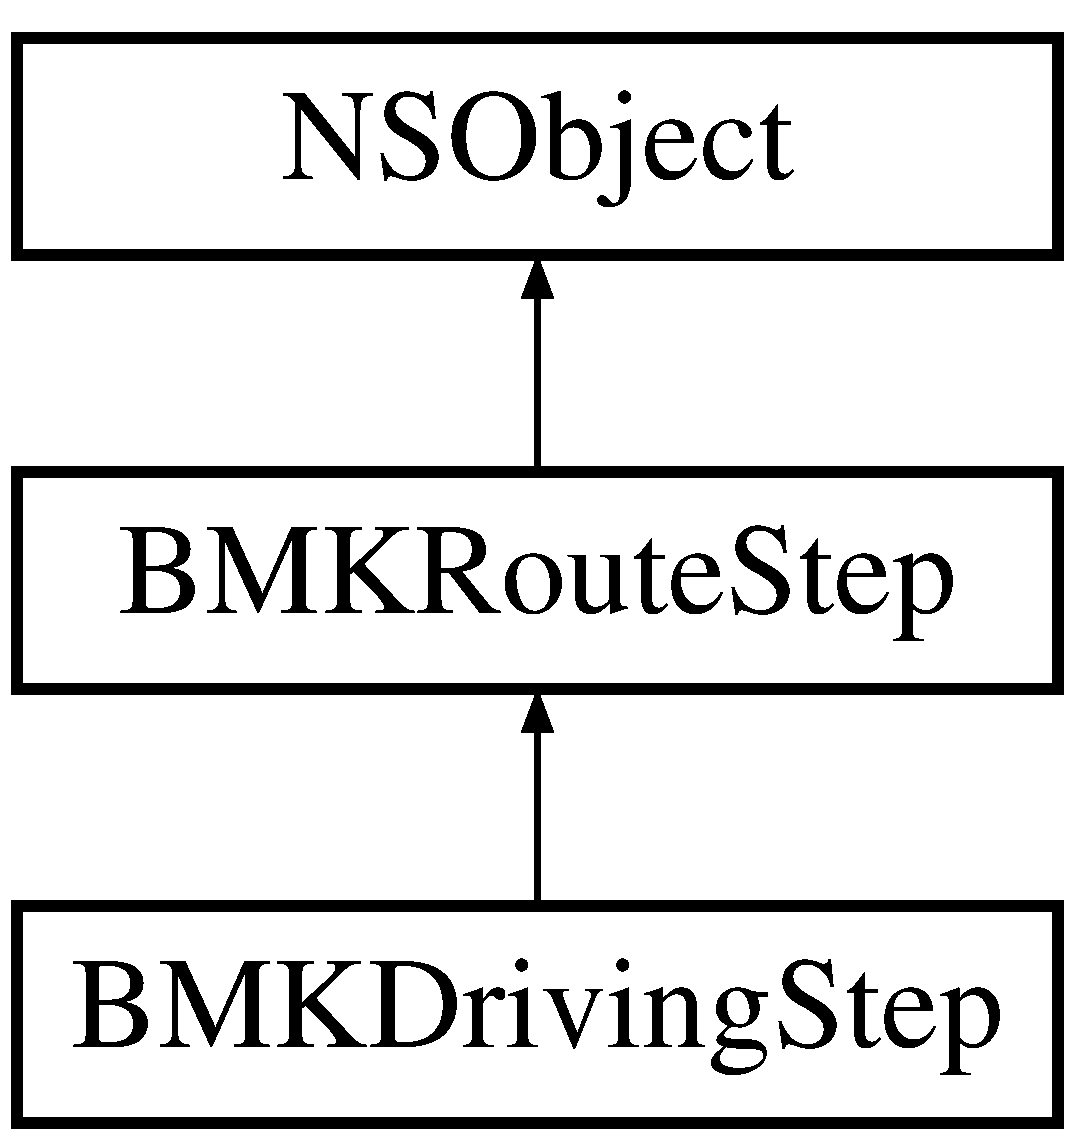
\includegraphics[height=3.000000cm]{interface_b_m_k_driving_step}
\end{center}
\end{figure}
\subsection*{Protected 属性}
\begin{DoxyCompactItemize}
\item 
\hypertarget{interface_b_m_k_driving_step_a5a13f3fe8c37bc2c59ce53918c4ba9e3}{int {\bfseries \+\_\+direction}}\label{interface_b_m_k_driving_step_a5a13f3fe8c37bc2c59ce53918c4ba9e3}

\item 
\hypertarget{interface_b_m_k_driving_step_ad9734de65efa299609b3e727cd54c0ee}{\hyperlink{interface_b_m_k_route_node}{B\+M\+K\+Route\+Node} $\ast$ {\bfseries \+\_\+entrace}}\label{interface_b_m_k_driving_step_ad9734de65efa299609b3e727cd54c0ee}

\item 
\hypertarget{interface_b_m_k_driving_step_a56fac51f78875aeab300b0b90beb000b}{N\+S\+String $\ast$ {\bfseries \+\_\+entrace\+Instruction}}\label{interface_b_m_k_driving_step_a56fac51f78875aeab300b0b90beb000b}

\item 
\hypertarget{interface_b_m_k_driving_step_a44388ed0ddfc2ea0ed3d618c4fae6bf6}{\hyperlink{interface_b_m_k_route_node}{B\+M\+K\+Route\+Node} $\ast$ {\bfseries \+\_\+exit}}\label{interface_b_m_k_driving_step_a44388ed0ddfc2ea0ed3d618c4fae6bf6}

\item 
\hypertarget{interface_b_m_k_driving_step_a1150eaac21b797ae0b22bec7776f7d84}{N\+S\+String $\ast$ {\bfseries \+\_\+exit\+Instruction}}\label{interface_b_m_k_driving_step_a1150eaac21b797ae0b22bec7776f7d84}

\item 
\hypertarget{interface_b_m_k_driving_step_a5d762f4cdd070e074ad0d18470b1e811}{N\+S\+String $\ast$ {\bfseries \+\_\+instruction}}\label{interface_b_m_k_driving_step_a5d762f4cdd070e074ad0d18470b1e811}

\item 
\hypertarget{interface_b_m_k_driving_step_a435b2806b650b115fdad649e9fd08feb}{int {\bfseries \+\_\+num\+Turns}}\label{interface_b_m_k_driving_step_a435b2806b650b115fdad649e9fd08feb}

\end{DoxyCompactItemize}
\subsection*{属性}
\begin{DoxyCompactItemize}
\item 
\hypertarget{interface_b_m_k_driving_step_a32f44a9d4e3bfb73a64a1ac0aa15df7e}{int \hyperlink{interface_b_m_k_driving_step_a32f44a9d4e3bfb73a64a1ac0aa15df7e}{direction}}\label{interface_b_m_k_driving_step_a32f44a9d4e3bfb73a64a1ac0aa15df7e}

\begin{DoxyCompactList}\small\item\em 该路段起点方向值 \end{DoxyCompactList}\item 
\hypertarget{interface_b_m_k_driving_step_aaebe4d99c4335c4995d819da68070675}{\hyperlink{interface_b_m_k_route_node}{B\+M\+K\+Route\+Node} $\ast$ \hyperlink{interface_b_m_k_driving_step_aaebe4d99c4335c4995d819da68070675}{entrace}}\label{interface_b_m_k_driving_step_aaebe4d99c4335c4995d819da68070675}

\begin{DoxyCompactList}\small\item\em 路段入口信息 \end{DoxyCompactList}\item 
\hypertarget{interface_b_m_k_driving_step_ac795c99a6fe1947752b037792682e29e}{N\+S\+String $\ast$ \hyperlink{interface_b_m_k_driving_step_ac795c99a6fe1947752b037792682e29e}{entrace\+Instruction}}\label{interface_b_m_k_driving_step_ac795c99a6fe1947752b037792682e29e}

\begin{DoxyCompactList}\small\item\em 路段入口的指示信息 \end{DoxyCompactList}\item 
\hypertarget{interface_b_m_k_driving_step_a18bb9a2457ed65f9c35f2026f45236aa}{\hyperlink{interface_b_m_k_route_node}{B\+M\+K\+Route\+Node} $\ast$ \hyperlink{interface_b_m_k_driving_step_a18bb9a2457ed65f9c35f2026f45236aa}{exit}}\label{interface_b_m_k_driving_step_a18bb9a2457ed65f9c35f2026f45236aa}

\begin{DoxyCompactList}\small\item\em 路段出口信息 \end{DoxyCompactList}\item 
\hypertarget{interface_b_m_k_driving_step_a2fd7d4885e56694283f0ed9d92d8b0cd}{N\+S\+String $\ast$ \hyperlink{interface_b_m_k_driving_step_a2fd7d4885e56694283f0ed9d92d8b0cd}{exit\+Instruction}}\label{interface_b_m_k_driving_step_a2fd7d4885e56694283f0ed9d92d8b0cd}

\begin{DoxyCompactList}\small\item\em 路段出口指示信息 \end{DoxyCompactList}\item 
\hypertarget{interface_b_m_k_driving_step_a70a35973fdc204236c21d44770014989}{N\+S\+String $\ast$ \hyperlink{interface_b_m_k_driving_step_a70a35973fdc204236c21d44770014989}{instruction}}\label{interface_b_m_k_driving_step_a70a35973fdc204236c21d44770014989}

\begin{DoxyCompactList}\small\item\em 路段总体指示信息 \end{DoxyCompactList}\item 
\hypertarget{interface_b_m_k_driving_step_a261507960f7fcf3b6981e9a31667f47c}{int \hyperlink{interface_b_m_k_driving_step_a261507960f7fcf3b6981e9a31667f47c}{num\+Turns}}\label{interface_b_m_k_driving_step_a261507960f7fcf3b6981e9a31667f47c}

\begin{DoxyCompactList}\small\item\em 路段需要转弯数 \end{DoxyCompactList}\end{DoxyCompactItemize}


\subsection{详细描述}
此类表示驾车路线中的一个路段 

该类的文档由以下文件生成\+:\begin{DoxyCompactItemize}
\item 
output/map\+\_\+search\+\_\+cloud\+\_\+loc\+\_\+util/inc/B\+M\+K\+Route\+Search\+Type.\+h\end{DoxyCompactItemize}

\hypertarget{protocol_b_m_k_general_delegate-p}{\section{$<$B\+M\+K\+General\+Delegate$>$协议 参考}
\label{protocol_b_m_k_general_delegate-p}\index{$<$\+B\+M\+K\+General\+Delegate$>$@{$<$\+B\+M\+K\+General\+Delegate$>$}}
}


通知\+Delegate  




{\ttfamily \#import $<$B\+M\+K\+General\+Delegate.\+h$>$}

类 $<$B\+M\+K\+General\+Delegate$>$ 继承关系图\+:\begin{figure}[H]
\begin{center}
\leavevmode
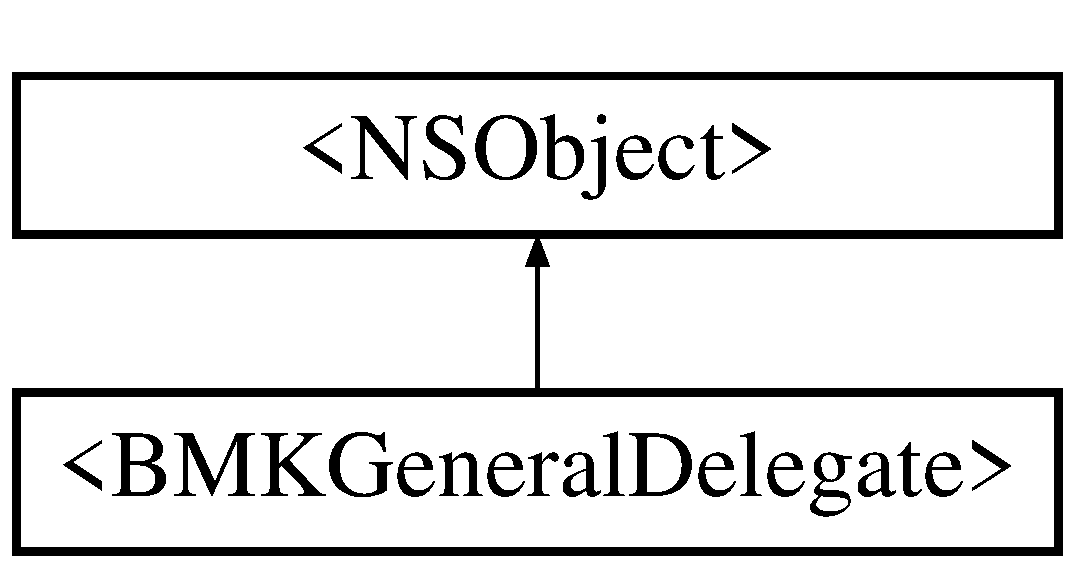
\includegraphics[height=2.000000cm]{protocol_b_m_k_general_delegate-p}
\end{center}
\end{figure}
\subsection*{Instance Methods}
\begin{DoxyCompactItemize}
\item 
(void) -\/ \hyperlink{protocol_b_m_k_general_delegate-p_ad30d0a4dc9bb54cda10cb892ed769491}{on\+Get\+Network\+State\+:}
\item 
(void) -\/ \hyperlink{protocol_b_m_k_general_delegate-p_ab0c34f007a8be34196fc81f2c7b3cddb}{on\+Get\+Permission\+State\+:}
\end{DoxyCompactItemize}


\subsection{详细描述}
通知\+Delegate 

\subsection{Method Documentation}
\hypertarget{protocol_b_m_k_general_delegate-p_ad30d0a4dc9bb54cda10cb892ed769491}{\index{B\+M\+K\+General\+Delegate-\/p@{B\+M\+K\+General\+Delegate-\/p}!on\+Get\+Network\+State\+:@{on\+Get\+Network\+State\+:}}
\index{on\+Get\+Network\+State\+:@{on\+Get\+Network\+State\+:}!B\+M\+K\+General\+Delegate-\/p@{B\+M\+K\+General\+Delegate-\/p}}
\subsubsection[{on\+Get\+Network\+State\+:}]{\setlength{\rightskip}{0pt plus 5cm}-\/ (void) on\+Get\+Network\+State\+: 
\begin{DoxyParamCaption}
\item[{(int)}]{i\+Error}
\end{DoxyParamCaption}
\hspace{0.3cm}{\ttfamily [optional]}}}\label{protocol_b_m_k_general_delegate-p_ad30d0a4dc9bb54cda10cb892ed769491}
返回网络错误 
\begin{DoxyParams}{参数}
{\em i\+Error} & 错误号 \\
\hline
\end{DoxyParams}
\hypertarget{protocol_b_m_k_general_delegate-p_ab0c34f007a8be34196fc81f2c7b3cddb}{\index{B\+M\+K\+General\+Delegate-\/p@{B\+M\+K\+General\+Delegate-\/p}!on\+Get\+Permission\+State\+:@{on\+Get\+Permission\+State\+:}}
\index{on\+Get\+Permission\+State\+:@{on\+Get\+Permission\+State\+:}!B\+M\+K\+General\+Delegate-\/p@{B\+M\+K\+General\+Delegate-\/p}}
\subsubsection[{on\+Get\+Permission\+State\+:}]{\setlength{\rightskip}{0pt plus 5cm}-\/ (void) on\+Get\+Permission\+State\+: 
\begin{DoxyParamCaption}
\item[{(int)}]{i\+Error}
\end{DoxyParamCaption}
\hspace{0.3cm}{\ttfamily [optional]}}}\label{protocol_b_m_k_general_delegate-p_ab0c34f007a8be34196fc81f2c7b3cddb}
返回授权验证错误 
\begin{DoxyParams}{参数}
{\em i\+Error} & 错误号 \+: 为0时验证通过,具体参加\+B\+M\+K\+Permission\+Check\+Result\+Code \\
\hline
\end{DoxyParams}


该协议的文档由以下文件生成\+:\begin{DoxyCompactItemize}
\item 
output/map\+\_\+search\+\_\+cloud\+\_\+loc\+\_\+util/inc/B\+M\+K\+General\+Delegate.\+h\end{DoxyCompactItemize}

\hypertarget{interface_b_m_k_geo_code_result}{\section{B\+M\+K\+Geo\+Code\+Result类 参考}
\label{interface_b_m_k_geo_code_result}\index{B\+M\+K\+Geo\+Code\+Result@{B\+M\+K\+Geo\+Code\+Result}}
}


地址编码结果  




{\ttfamily \#import $<$B\+M\+K\+Geocode\+Type.\+h$>$}

类 B\+M\+K\+Geo\+Code\+Result 继承关系图\+:\begin{figure}[H]
\begin{center}
\leavevmode
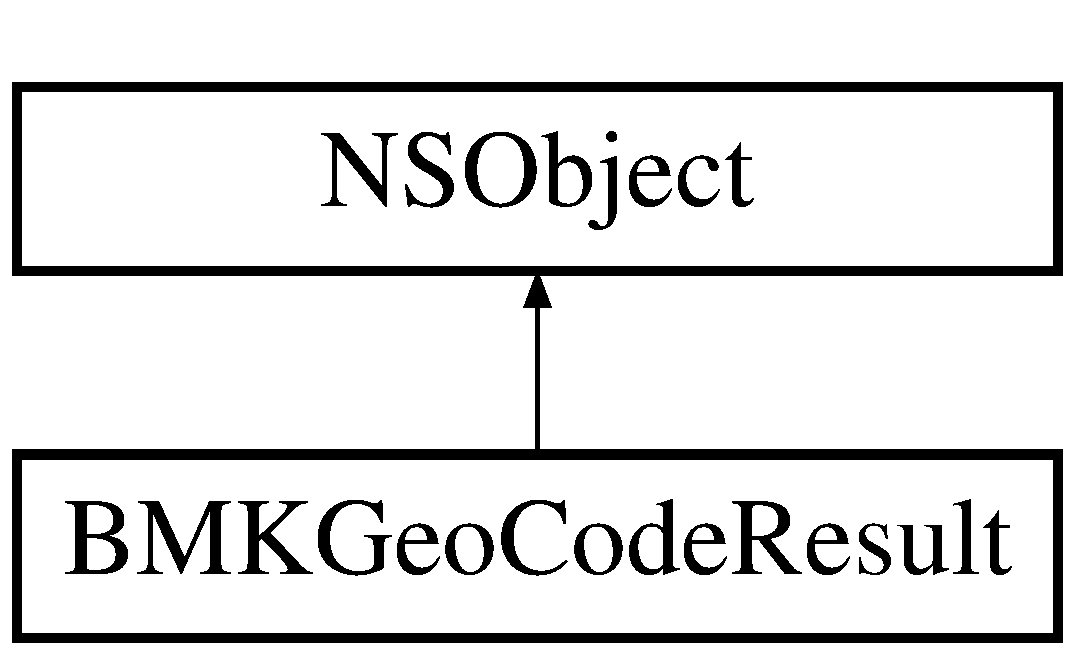
\includegraphics[height=2.000000cm]{interface_b_m_k_geo_code_result}
\end{center}
\end{figure}
\subsection*{Protected 属性}
\begin{DoxyCompactItemize}
\item 
\hypertarget{interface_b_m_k_geo_code_result_a24d63bcf89a08aaf8d2c74bfbbcf3f41}{C\+L\+Location\+Coordinate2\+D {\bfseries \+\_\+location}}\label{interface_b_m_k_geo_code_result_a24d63bcf89a08aaf8d2c74bfbbcf3f41}

\item 
\hypertarget{interface_b_m_k_geo_code_result_a7d9c5ba3e65ea13e9787ba3c00273f1c}{N\+S\+String $\ast$ {\bfseries \+\_\+address}}\label{interface_b_m_k_geo_code_result_a7d9c5ba3e65ea13e9787ba3c00273f1c}

\end{DoxyCompactItemize}
\subsection*{属性}
\begin{DoxyCompactItemize}
\item 
\hypertarget{interface_b_m_k_geo_code_result_a4f2aaf9561f955a26979d388557ff31b}{C\+L\+Location\+Coordinate2\+D \hyperlink{interface_b_m_k_geo_code_result_a4f2aaf9561f955a26979d388557ff31b}{location}}\label{interface_b_m_k_geo_code_result_a4f2aaf9561f955a26979d388557ff31b}

\begin{DoxyCompactList}\small\item\em 地理编码位置 \end{DoxyCompactList}\item 
\hypertarget{interface_b_m_k_geo_code_result_a828c8d7063323c1540e9d66bdf0df22c}{N\+S\+String $\ast$ \hyperlink{interface_b_m_k_geo_code_result_a828c8d7063323c1540e9d66bdf0df22c}{address}}\label{interface_b_m_k_geo_code_result_a828c8d7063323c1540e9d66bdf0df22c}

\begin{DoxyCompactList}\small\item\em 地理编码地址 \end{DoxyCompactList}\end{DoxyCompactItemize}


\subsection{详细描述}
地址编码结果 

该类的文档由以下文件生成\+:\begin{DoxyCompactItemize}
\item 
output/map\+\_\+search\+\_\+cloud\+\_\+loc\+\_\+util/inc/B\+M\+K\+Geocode\+Type.\+h\end{DoxyCompactItemize}

\hypertarget{interface_b_m_k_geo_code_search}{\section{B\+M\+K\+Geo\+Code\+Search类 参考}
\label{interface_b_m_k_geo_code_search}\index{B\+M\+K\+Geo\+Code\+Search@{B\+M\+K\+Geo\+Code\+Search}}
}


geo搜索服务  




{\ttfamily \#import $<$B\+M\+K\+Geocode\+Search.\+h$>$}

类 B\+M\+K\+Geo\+Code\+Search 继承关系图\+:\begin{figure}[H]
\begin{center}
\leavevmode
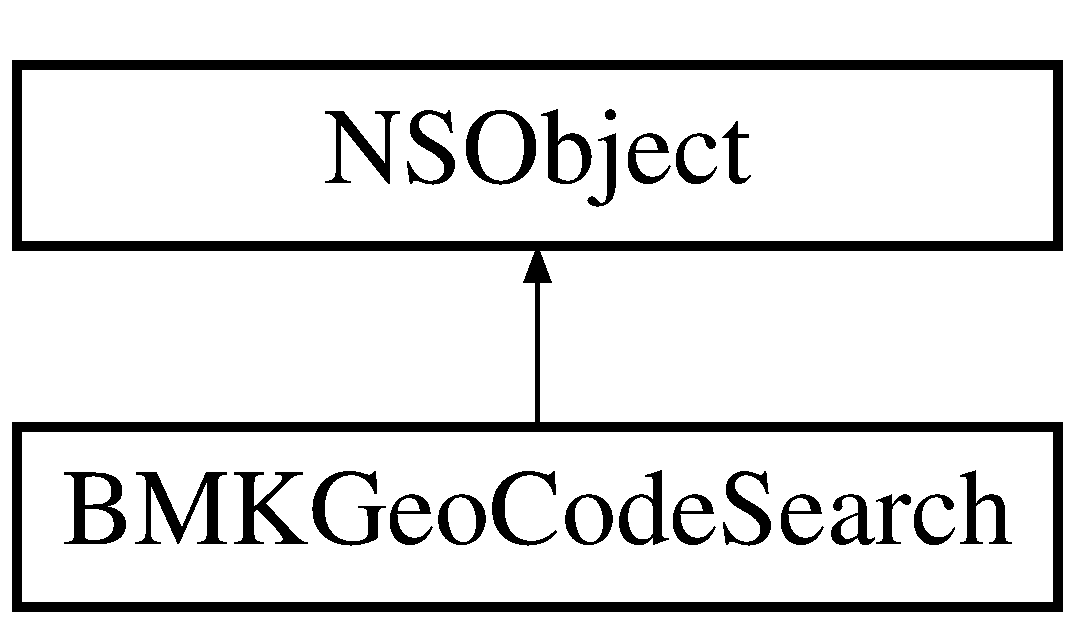
\includegraphics[height=2.000000cm]{interface_b_m_k_geo_code_search}
\end{center}
\end{figure}
\subsection*{Instance Methods}
\begin{DoxyCompactItemize}
\item 
(B\+O\+O\+L) -\/ \hyperlink{interface_b_m_k_geo_code_search_a48248533fdf98ee24679d97716f6d55b}{geo\+Code\+:}
\item 
(B\+O\+O\+L) -\/ \hyperlink{interface_b_m_k_geo_code_search_a3594336ed6a95074f069b4d0ebc75df2}{reverse\+Geo\+Code\+:}
\end{DoxyCompactItemize}
\subsection*{属性}
\begin{DoxyCompactItemize}
\item 
\hypertarget{interface_b_m_k_geo_code_search_a7a816dcf6d4f679ad3287948ad9427d2}{id$<$ \hyperlink{protocol_b_m_k_geo_code_search_delegate-p}{B\+M\+K\+Geo\+Code\+Search\+Delegate} $>$ \hyperlink{interface_b_m_k_geo_code_search_a7a816dcf6d4f679ad3287948ad9427d2}{delegate}}\label{interface_b_m_k_geo_code_search_a7a816dcf6d4f679ad3287948ad9427d2}

\begin{DoxyCompactList}\small\item\em 检索模块的\+Delegate,此处记得不用的时候需要置nil,否则影响内存的释放 \end{DoxyCompactList}\end{DoxyCompactItemize}


\subsection{详细描述}
geo搜索服务 

\subsection{Method Documentation}
\hypertarget{interface_b_m_k_geo_code_search_a48248533fdf98ee24679d97716f6d55b}{\index{B\+M\+K\+Geo\+Code\+Search@{B\+M\+K\+Geo\+Code\+Search}!geo\+Code\+:@{geo\+Code\+:}}
\index{geo\+Code\+:@{geo\+Code\+:}!B\+M\+K\+Geo\+Code\+Search@{B\+M\+K\+Geo\+Code\+Search}}
\subsubsection[{geo\+Code\+:}]{\setlength{\rightskip}{0pt plus 5cm}-\/ (B\+O\+O\+L) geo\+Code\+: 
\begin{DoxyParamCaption}
\item[{({\bf B\+M\+K\+Geo\+Code\+Search\+Option} $\ast$)}]{geo\+Code\+Option}
\end{DoxyParamCaption}
}}\label{interface_b_m_k_geo_code_search_a48248533fdf98ee24679d97716f6d55b}
根据地址名称获取地理信息 异步函数,返回结果在\+B\+M\+K\+Geo\+Code\+Search\+Delegate的on\+Get\+Addr\+Result通知 
\begin{DoxyParams}{参数}
{\em geo\+Code\+Option} & geo检索信息类 \\
\hline
\end{DoxyParams}
\begin{DoxyReturn}{返回}
成功返回\+Y\+E\+S,否则返回\+N\+O 
\end{DoxyReturn}
\hypertarget{interface_b_m_k_geo_code_search_a3594336ed6a95074f069b4d0ebc75df2}{\index{B\+M\+K\+Geo\+Code\+Search@{B\+M\+K\+Geo\+Code\+Search}!reverse\+Geo\+Code\+:@{reverse\+Geo\+Code\+:}}
\index{reverse\+Geo\+Code\+:@{reverse\+Geo\+Code\+:}!B\+M\+K\+Geo\+Code\+Search@{B\+M\+K\+Geo\+Code\+Search}}
\subsubsection[{reverse\+Geo\+Code\+:}]{\setlength{\rightskip}{0pt plus 5cm}-\/ (B\+O\+O\+L) reverse\+Geo\+Code\+: 
\begin{DoxyParamCaption}
\item[{({\bf B\+M\+K\+Reverse\+Geo\+Code\+Option} $\ast$)}]{reverse\+Geo\+Code\+Option}
\end{DoxyParamCaption}
}}\label{interface_b_m_k_geo_code_search_a3594336ed6a95074f069b4d0ebc75df2}
根据地理坐标获取地址信息 异步函数,返回结果在\+B\+M\+K\+Geo\+Code\+Search\+Delegate的on\+Get\+Addr\+Result通知 
\begin{DoxyParams}{参数}
{\em reverse\+Geo\+Code\+Option} & 反geo检索信息类 \\
\hline
\end{DoxyParams}
\begin{DoxyReturn}{返回}
成功返回\+Y\+E\+S,否则返回\+N\+O 
\end{DoxyReturn}


该类的文档由以下文件生成\+:\begin{DoxyCompactItemize}
\item 
output/map\+\_\+search\+\_\+cloud\+\_\+loc\+\_\+util/inc/B\+M\+K\+Geocode\+Search.\+h\end{DoxyCompactItemize}

\hypertarget{protocol_b_m_k_geo_code_search_delegate-p}{\section{$<$B\+M\+K\+Geo\+Code\+Search\+Delegate$>$协议 参考}
\label{protocol_b_m_k_geo_code_search_delegate-p}\index{$<$\+B\+M\+K\+Geo\+Code\+Search\+Delegate$>$@{$<$\+B\+M\+K\+Geo\+Code\+Search\+Delegate$>$}}
}


搜索delegate,用于获取搜索结果  




{\ttfamily \#import $<$B\+M\+K\+Geocode\+Search.\+h$>$}

类 $<$B\+M\+K\+Geo\+Code\+Search\+Delegate$>$ 继承关系图\+:\begin{figure}[H]
\begin{center}
\leavevmode
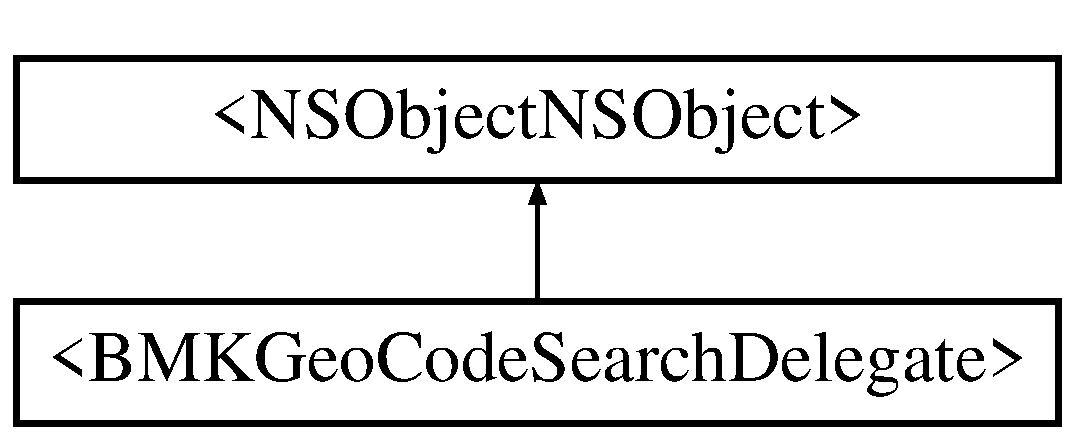
\includegraphics[height=2.000000cm]{protocol_b_m_k_geo_code_search_delegate-p}
\end{center}
\end{figure}
\subsection*{Instance Methods}
\begin{DoxyCompactItemize}
\item 
(void) -\/ \hyperlink{protocol_b_m_k_geo_code_search_delegate-p_ac50237b58058d88d46ad0a4c99208382}{on\+Get\+Geo\+Code\+Result\+:result\+:error\+Code\+:}
\item 
(void) -\/ \hyperlink{protocol_b_m_k_geo_code_search_delegate-p_a8b9139623a45d9366e38bd000c1369c0}{on\+Get\+Reverse\+Geo\+Code\+Result\+:result\+:error\+Code\+:}
\end{DoxyCompactItemize}


\subsection{详细描述}
搜索delegate,用于获取搜索结果 

\subsection{Method Documentation}
\hypertarget{protocol_b_m_k_geo_code_search_delegate-p_ac50237b58058d88d46ad0a4c99208382}{\index{B\+M\+K\+Geo\+Code\+Search\+Delegate-\/p@{B\+M\+K\+Geo\+Code\+Search\+Delegate-\/p}!on\+Get\+Geo\+Code\+Result\+:result\+:error\+Code\+:@{on\+Get\+Geo\+Code\+Result\+:result\+:error\+Code\+:}}
\index{on\+Get\+Geo\+Code\+Result\+:result\+:error\+Code\+:@{on\+Get\+Geo\+Code\+Result\+:result\+:error\+Code\+:}!B\+M\+K\+Geo\+Code\+Search\+Delegate-\/p@{B\+M\+K\+Geo\+Code\+Search\+Delegate-\/p}}
\subsubsection[{on\+Get\+Geo\+Code\+Result\+:result\+:error\+Code\+:}]{\setlength{\rightskip}{0pt plus 5cm}-\/ (void) on\+Get\+Geo\+Code\+Result\+: 
\begin{DoxyParamCaption}
\item[{({\bf B\+M\+K\+Geo\+Code\+Search} $\ast$)}]{searcher}
\item[{result:({\bf B\+M\+K\+Geo\+Code\+Result} $\ast$)}]{result}
\item[{errorCode:(B\+M\+K\+Search\+Error\+Code)}]{error}
\end{DoxyParamCaption}
\hspace{0.3cm}{\ttfamily [optional]}}}\label{protocol_b_m_k_geo_code_search_delegate-p_ac50237b58058d88d46ad0a4c99208382}
返回地址信息搜索结果 
\begin{DoxyParams}{参数}
{\em searcher} & 搜索对象 \\
\hline
{\em result} & 搜索结\+B\+M\+K\+Geo\+Code\+Search果 \\
\hline
{\em error} & 错误号,\\
\hline
\end{DoxyParams}
\begin{DoxySeeAlso}{参见}
B\+M\+K\+Search\+Error\+Code 
\end{DoxySeeAlso}
\hypertarget{protocol_b_m_k_geo_code_search_delegate-p_a8b9139623a45d9366e38bd000c1369c0}{\index{B\+M\+K\+Geo\+Code\+Search\+Delegate-\/p@{B\+M\+K\+Geo\+Code\+Search\+Delegate-\/p}!on\+Get\+Reverse\+Geo\+Code\+Result\+:result\+:error\+Code\+:@{on\+Get\+Reverse\+Geo\+Code\+Result\+:result\+:error\+Code\+:}}
\index{on\+Get\+Reverse\+Geo\+Code\+Result\+:result\+:error\+Code\+:@{on\+Get\+Reverse\+Geo\+Code\+Result\+:result\+:error\+Code\+:}!B\+M\+K\+Geo\+Code\+Search\+Delegate-\/p@{B\+M\+K\+Geo\+Code\+Search\+Delegate-\/p}}
\subsubsection[{on\+Get\+Reverse\+Geo\+Code\+Result\+:result\+:error\+Code\+:}]{\setlength{\rightskip}{0pt plus 5cm}-\/ (void) on\+Get\+Reverse\+Geo\+Code\+Result\+: 
\begin{DoxyParamCaption}
\item[{({\bf B\+M\+K\+Geo\+Code\+Search} $\ast$)}]{searcher}
\item[{result:({\bf B\+M\+K\+Reverse\+Geo\+Code\+Result} $\ast$)}]{result}
\item[{errorCode:(B\+M\+K\+Search\+Error\+Code)}]{error}
\end{DoxyParamCaption}
\hspace{0.3cm}{\ttfamily [optional]}}}\label{protocol_b_m_k_geo_code_search_delegate-p_a8b9139623a45d9366e38bd000c1369c0}
返回反地理编码搜索结果 
\begin{DoxyParams}{参数}
{\em searcher} & 搜索对象 \\
\hline
{\em result} & 搜索结果 \\
\hline
{\em error} & 错误号,\\
\hline
\end{DoxyParams}
\begin{DoxySeeAlso}{参见}
B\+M\+K\+Search\+Error\+Code 
\end{DoxySeeAlso}


该协议的文档由以下文件生成\+:\begin{DoxyCompactItemize}
\item 
output/map\+\_\+search\+\_\+cloud\+\_\+loc\+\_\+util/inc/B\+M\+K\+Geocode\+Search.\+h\end{DoxyCompactItemize}

\hypertarget{interface_b_m_k_geo_code_search_option}{\section{B\+M\+K\+Geo\+Code\+Search\+Option类 参考}
\label{interface_b_m_k_geo_code_search_option}\index{B\+M\+K\+Geo\+Code\+Search\+Option@{B\+M\+K\+Geo\+Code\+Search\+Option}}
}


geo检索信息类  




{\ttfamily \#import $<$B\+M\+K\+Geocode\+Search\+Option.\+h$>$}

类 B\+M\+K\+Geo\+Code\+Search\+Option 继承关系图\+:\begin{figure}[H]
\begin{center}
\leavevmode
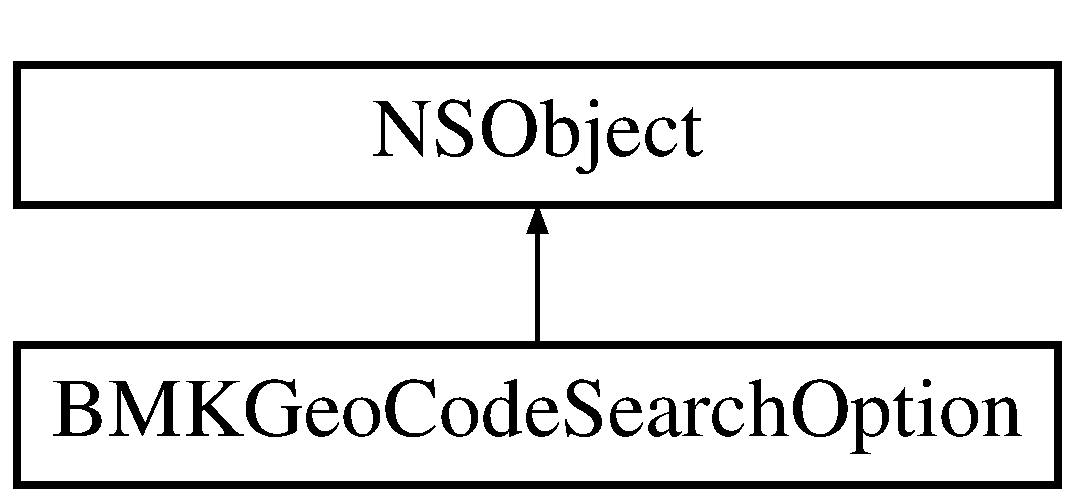
\includegraphics[height=2.000000cm]{interface_b_m_k_geo_code_search_option}
\end{center}
\end{figure}
\subsection*{Protected 属性}
\begin{DoxyCompactItemize}
\item 
\hypertarget{interface_b_m_k_geo_code_search_option_ad60b7404c92ec2b83741da90bd9c6375}{N\+S\+String $\ast$ {\bfseries \+\_\+address}}\label{interface_b_m_k_geo_code_search_option_ad60b7404c92ec2b83741da90bd9c6375}

\item 
\hypertarget{interface_b_m_k_geo_code_search_option_a3cd2ae3510249ea055adaa246e7947c3}{N\+S\+String $\ast$ {\bfseries \+\_\+city}}\label{interface_b_m_k_geo_code_search_option_a3cd2ae3510249ea055adaa246e7947c3}

\end{DoxyCompactItemize}
\subsection*{属性}
\begin{DoxyCompactItemize}
\item 
\hypertarget{interface_b_m_k_geo_code_search_option_a8d27ba1022cbb8b24e0e4f7ab7ec8a46}{N\+S\+String $\ast$ \hyperlink{interface_b_m_k_geo_code_search_option_a8d27ba1022cbb8b24e0e4f7ab7ec8a46}{address}}\label{interface_b_m_k_geo_code_search_option_a8d27ba1022cbb8b24e0e4f7ab7ec8a46}

\begin{DoxyCompactList}\small\item\em 地址 \end{DoxyCompactList}\item 
\hypertarget{interface_b_m_k_geo_code_search_option_ad16f0f623de2a8a74114fb72b2844003}{N\+S\+String $\ast$ \hyperlink{interface_b_m_k_geo_code_search_option_ad16f0f623de2a8a74114fb72b2844003}{city}}\label{interface_b_m_k_geo_code_search_option_ad16f0f623de2a8a74114fb72b2844003}

\begin{DoxyCompactList}\small\item\em 城市名 \end{DoxyCompactList}\end{DoxyCompactItemize}


\subsection{详细描述}
geo检索信息类 

该类的文档由以下文件生成\+:\begin{DoxyCompactItemize}
\item 
output/map\+\_\+search\+\_\+cloud\+\_\+loc\+\_\+util/inc/B\+M\+K\+Geocode\+Search\+Option.\+h\end{DoxyCompactItemize}

\hypertarget{struct_b_m_k_geo_point}{\section{B\+M\+K\+Geo\+Point结构体 参考}
\label{struct_b_m_k_geo_point}\index{B\+M\+K\+Geo\+Point@{B\+M\+K\+Geo\+Point}}
}


表示一个经纬度坐标点  




{\ttfamily \#include $<$B\+M\+K\+Types.\+h$>$}

\subsection*{Public 属性}
\begin{DoxyCompactItemize}
\item 
\hypertarget{struct_b_m_k_geo_point_ad6f5b38335cff314e953e9b7eb5c7b39}{int \hyperlink{struct_b_m_k_geo_point_ad6f5b38335cff314e953e9b7eb5c7b39}{latitude\+E6}}\label{struct_b_m_k_geo_point_ad6f5b38335cff314e953e9b7eb5c7b39}

\begin{DoxyCompactList}\small\item\em 纬度,乘以1e6之后的值 \end{DoxyCompactList}\item 
\hypertarget{struct_b_m_k_geo_point_aac3f3dc0ae09785e5b70c319b68d4047}{int \hyperlink{struct_b_m_k_geo_point_aac3f3dc0ae09785e5b70c319b68d4047}{longitude\+E6}}\label{struct_b_m_k_geo_point_aac3f3dc0ae09785e5b70c319b68d4047}

\begin{DoxyCompactList}\small\item\em 经度,乘以1e6之后的值 \end{DoxyCompactList}\end{DoxyCompactItemize}


\subsection{详细描述}
表示一个经纬度坐标点 

该结构体的文档由以下文件生成\+:\begin{DoxyCompactItemize}
\item 
output/map\+\_\+search\+\_\+cloud\+\_\+loc\+\_\+util/inc/B\+M\+K\+Types.\+h\end{DoxyCompactItemize}

\hypertarget{interface_b_m_k_gradient}{\section{B\+M\+K\+Gradient类 参考}
\label{interface_b_m_k_gradient}\index{B\+M\+K\+Gradient@{B\+M\+K\+Gradient}}
}


此类表示热力图渐变色  




{\ttfamily \#import $<$B\+M\+K\+Gradient.\+h$>$}

类 B\+M\+K\+Gradient 继承关系图\+:\begin{figure}[H]
\begin{center}
\leavevmode
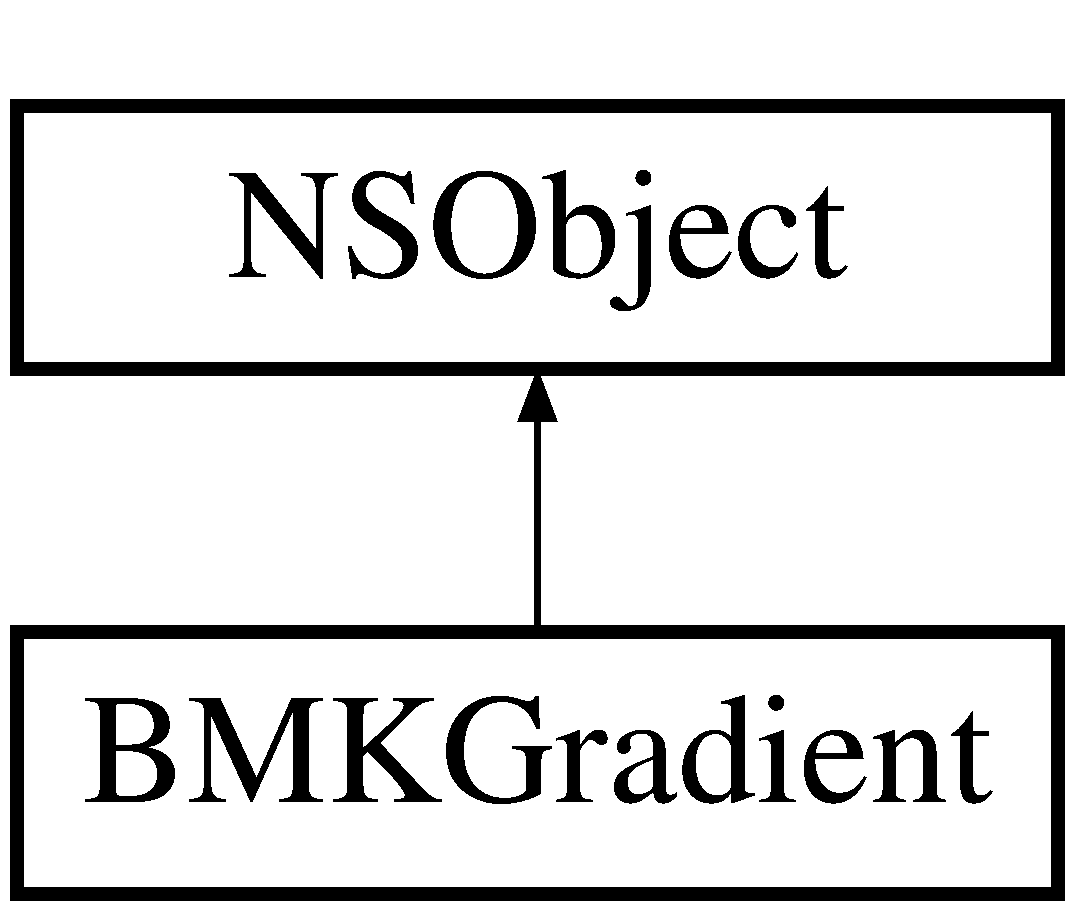
\includegraphics[height=2.000000cm]{interface_b_m_k_gradient}
\end{center}
\end{figure}
\subsection*{Instance Methods}
\begin{DoxyCompactItemize}
\item 
\hypertarget{interface_b_m_k_gradient_af4c887250c744cdfb9f472846449d05b}{(id) -\/ {\bfseries init\+With\+Colors\+:start\+Points\+:}}\label{interface_b_m_k_gradient_af4c887250c744cdfb9f472846449d05b}

\end{DoxyCompactItemize}
\subsection*{属性}
\begin{DoxyCompactItemize}
\item 
\hypertarget{interface_b_m_k_gradient_a74426351e0f774b497b5bc6848c4c97e}{N\+S\+Array $\ast$ \hyperlink{interface_b_m_k_gradient_a74426351e0f774b497b5bc6848c4c97e}{m\+Colors}}\label{interface_b_m_k_gradient_a74426351e0f774b497b5bc6848c4c97e}

\begin{DoxyCompactList}\small\item\em 渐变色用到的所有颜色数组,数组成员类型为\+U\+I\+Color \end{DoxyCompactList}\item 
\hypertarget{interface_b_m_k_gradient_aa26241e329d659f2cadcf2452a7371c6}{N\+S\+Array $\ast$ \hyperlink{interface_b_m_k_gradient_aa26241e329d659f2cadcf2452a7371c6}{m\+Start\+Points}}\label{interface_b_m_k_gradient_aa26241e329d659f2cadcf2452a7371c6}

\begin{DoxyCompactList}\small\item\em 每一个颜色的起始点数组,,数组成员类型为 \mbox{[}0,1\mbox{]}的double值, given as a percentage of the maximum intensity,个数和m\+Colors的个数必须相同,数组内元素必须时递增的 \end{DoxyCompactList}\end{DoxyCompactItemize}


\subsection{详细描述}
此类表示热力图渐变色 

该类的文档由以下文件生成\+:\begin{DoxyCompactItemize}
\item 
output/map\+\_\+search\+\_\+cloud\+\_\+loc\+\_\+util/inc/B\+M\+K\+Gradient.\+h\end{DoxyCompactItemize}

\hypertarget{interface_b_m_k_ground_overlay_view}{\section{B\+M\+K\+Ground\+Overlay\+View类 参考}
\label{interface_b_m_k_ground_overlay_view}\index{B\+M\+K\+Ground\+Overlay\+View@{B\+M\+K\+Ground\+Overlay\+View}}
}


该类用于定义一个\+B\+M\+K\+Ground\+Overlay\+View  




{\ttfamily \#import $<$B\+M\+K\+Ground\+Overlay\+View.\+h$>$}

类 B\+M\+K\+Ground\+Overlay\+View 继承关系图\+:\begin{figure}[H]
\begin{center}
\leavevmode
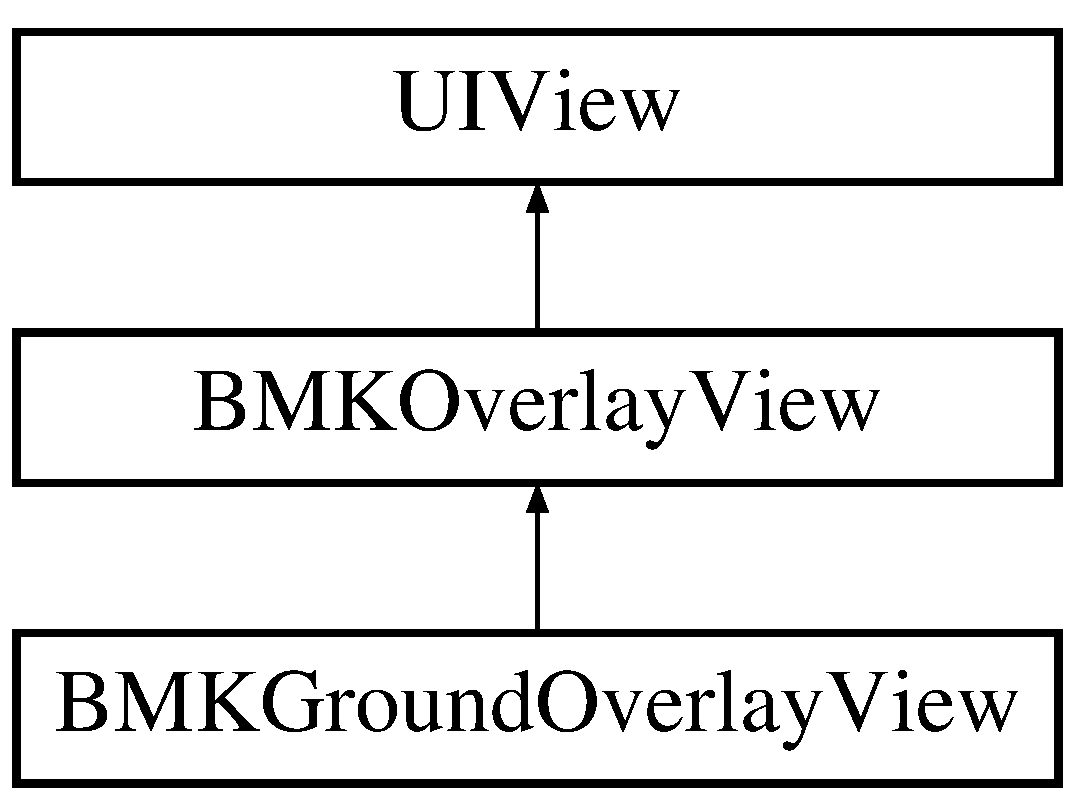
\includegraphics[height=3.000000cm]{interface_b_m_k_ground_overlay_view}
\end{center}
\end{figure}
\subsection*{Instance Methods}
\begin{DoxyCompactItemize}
\item 
(id) -\/ \hyperlink{interface_b_m_k_ground_overlay_view_a9a2e7f5341b40608aff7e8e70f219800}{init\+With\+Ground\+Overlay\+:}
\end{DoxyCompactItemize}
\subsection*{属性}
\begin{DoxyCompactItemize}
\item 
\hypertarget{interface_b_m_k_ground_overlay_view_afe3e5c81b5ba3b9a47dda8d3593fd8f2}{B\+M\+K\+Ground\+Overlay $\ast$ \hyperlink{interface_b_m_k_ground_overlay_view_afe3e5c81b5ba3b9a47dda8d3593fd8f2}{ground\+Overlay}}\label{interface_b_m_k_ground_overlay_view_afe3e5c81b5ba3b9a47dda8d3593fd8f2}

\begin{DoxyCompactList}\small\item\em 该\+View对应的ground数据对象 \end{DoxyCompactList}\end{DoxyCompactItemize}
\subsection*{额外继承的成员函数}


\subsection{详细描述}
该类用于定义一个\+B\+M\+K\+Ground\+Overlay\+View 

\subsection{Method Documentation}
\hypertarget{interface_b_m_k_ground_overlay_view_a9a2e7f5341b40608aff7e8e70f219800}{\index{B\+M\+K\+Ground\+Overlay\+View@{B\+M\+K\+Ground\+Overlay\+View}!init\+With\+Ground\+Overlay\+:@{init\+With\+Ground\+Overlay\+:}}
\index{init\+With\+Ground\+Overlay\+:@{init\+With\+Ground\+Overlay\+:}!B\+M\+K\+Ground\+Overlay\+View@{B\+M\+K\+Ground\+Overlay\+View}}
\subsubsection[{init\+With\+Ground\+Overlay\+:}]{\setlength{\rightskip}{0pt plus 5cm}-\/ (id) init\+With\+Ground\+Overlay\+: 
\begin{DoxyParamCaption}
\item[{(B\+M\+K\+Ground\+Overlay $\ast$)}]{ground\+Overlay}
\end{DoxyParamCaption}
}}\label{interface_b_m_k_ground_overlay_view_a9a2e7f5341b40608aff7e8e70f219800}
根据指定的ground\+Overlay生成一个\+View 
\begin{DoxyParams}{参数}
{\em ground\+Overlay} & 指定的ground\+Overlay数据对象 \\
\hline
\end{DoxyParams}
\begin{DoxyReturn}{返回}
新生成的\+View 
\end{DoxyReturn}


该类的文档由以下文件生成\+:\begin{DoxyCompactItemize}
\item 
output/map\+\_\+search\+\_\+cloud\+\_\+loc\+\_\+util/inc/B\+M\+K\+Ground\+Overlay\+View.\+h\end{DoxyCompactItemize}

\hypertarget{interface_b_m_k_heat_map}{\section{B\+M\+K\+Heat\+Map类 参考}
\label{interface_b_m_k_heat_map}\index{B\+M\+K\+Heat\+Map@{B\+M\+K\+Heat\+Map}}
}


热力图的绘制数据和显示样式类  




{\ttfamily \#import $<$B\+M\+K\+Heat\+Map.\+h$>$}

类 B\+M\+K\+Heat\+Map 继承关系图\+:\begin{figure}[H]
\begin{center}
\leavevmode
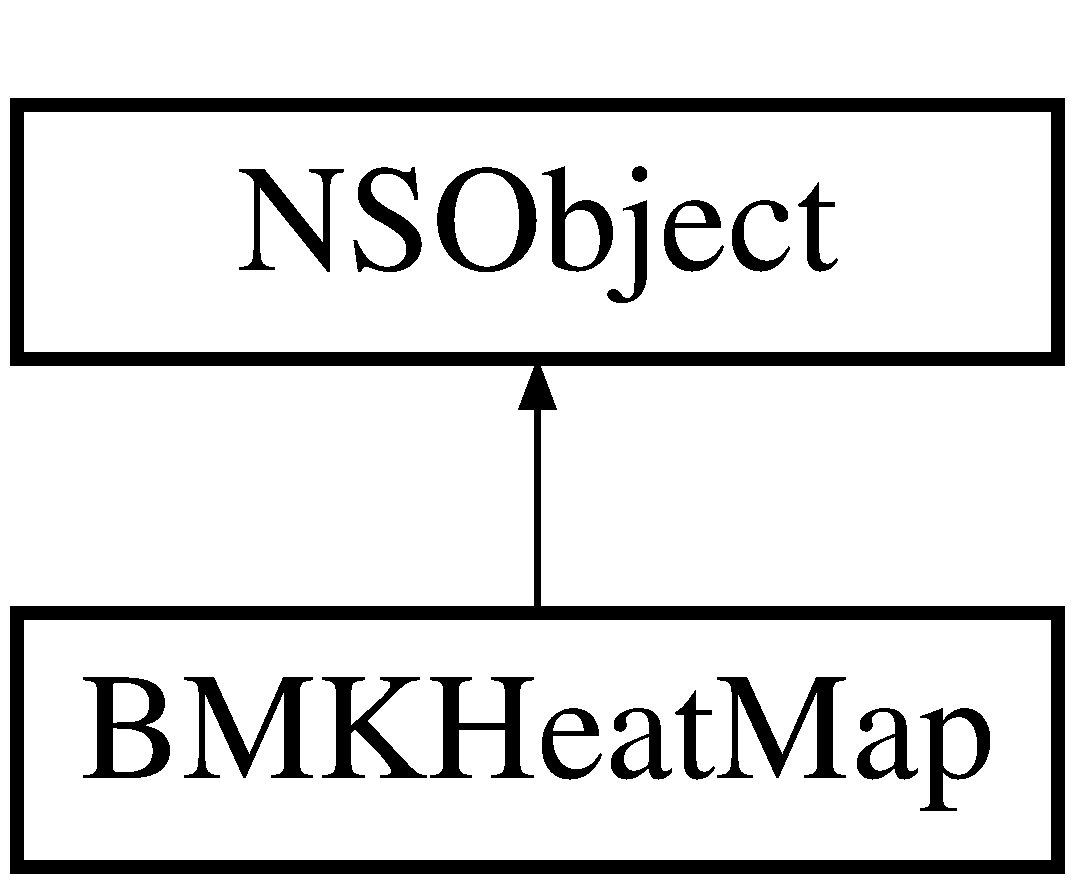
\includegraphics[height=2.000000cm]{interface_b_m_k_heat_map}
\end{center}
\end{figure}
\subsection*{Protected 属性}
\begin{DoxyCompactItemize}
\item 
\hypertarget{interface_b_m_k_heat_map_a70ff8c509134292bfd1b111196041085}{int {\bfseries \+\_\+m\+Radius}}\label{interface_b_m_k_heat_map_a70ff8c509134292bfd1b111196041085}

\item 
\hypertarget{interface_b_m_k_heat_map_a5cb9c9b8c4e4abad710abca27b2b3ec1}{\hyperlink{interface_b_m_k_gradient}{B\+M\+K\+Gradient} $\ast$ {\bfseries \+\_\+m\+Gradient}}\label{interface_b_m_k_heat_map_a5cb9c9b8c4e4abad710abca27b2b3ec1}

\item 
\hypertarget{interface_b_m_k_heat_map_ab1a2aac49094b1fb6c53ab09f9fc999d}{double {\bfseries \+\_\+m\+Opacity}}\label{interface_b_m_k_heat_map_ab1a2aac49094b1fb6c53ab09f9fc999d}

\item 
\hypertarget{interface_b_m_k_heat_map_a201c72e6cb01fec1eb1af4315b2508ba}{N\+S\+Mutable\+Array $\ast$ {\bfseries \+\_\+m\+Data}}\label{interface_b_m_k_heat_map_a201c72e6cb01fec1eb1af4315b2508ba}

\end{DoxyCompactItemize}
\subsection*{属性}
\begin{DoxyCompactItemize}
\item 
\hypertarget{interface_b_m_k_heat_map_a3e1a824fe5eb272797ac9b39cc596519}{int \hyperlink{interface_b_m_k_heat_map_a3e1a824fe5eb272797ac9b39cc596519}{m\+Radius}}\label{interface_b_m_k_heat_map_a3e1a824fe5eb272797ac9b39cc596519}

\begin{DoxyCompactList}\small\item\em 设置热力图点半径,默认为12ps \end{DoxyCompactList}\item 
\hypertarget{interface_b_m_k_heat_map_a2457a3c31731e42bfba4d17e4c83801f}{\hyperlink{interface_b_m_k_gradient}{B\+M\+K\+Gradient} $\ast$ \hyperlink{interface_b_m_k_heat_map_a2457a3c31731e42bfba4d17e4c83801f}{m\+Gradient}}\label{interface_b_m_k_heat_map_a2457a3c31731e42bfba4d17e4c83801f}

\begin{DoxyCompactList}\small\item\em 设置热力图渐变,有默认值 D\+E\+F\+A\+U\+L\+T\+\_\+\+G\+R\+A\+D\+I\+E\+N\+T \end{DoxyCompactList}\item 
\hypertarget{interface_b_m_k_heat_map_aa012e076b6487c0670499f61e8fe807f}{double \hyperlink{interface_b_m_k_heat_map_aa012e076b6487c0670499f61e8fe807f}{m\+Opacity}}\label{interface_b_m_k_heat_map_aa012e076b6487c0670499f61e8fe807f}

\begin{DoxyCompactList}\small\item\em 设置热力图层透明度,默认 0.\+6 \end{DoxyCompactList}\item 
\hypertarget{interface_b_m_k_heat_map_aa433ebe06960ff584026d8d2d191a6fe}{N\+S\+Mutable\+Array $\ast$ \hyperlink{interface_b_m_k_heat_map_aa433ebe06960ff584026d8d2d191a6fe}{m\+Data}}\label{interface_b_m_k_heat_map_aa433ebe06960ff584026d8d2d191a6fe}

\begin{DoxyCompactList}\small\item\em 用户传入的热力图数据,数组,成员类型为\+B\+M\+K\+Heat\+Map\+Node \end{DoxyCompactList}\end{DoxyCompactItemize}


\subsection{详细描述}
热力图的绘制数据和显示样式类 

该类的文档由以下文件生成\+:\begin{DoxyCompactItemize}
\item 
output/map\+\_\+search\+\_\+cloud\+\_\+loc\+\_\+util/inc/B\+M\+K\+Heat\+Map.\+h\end{DoxyCompactItemize}

\hypertarget{interface_b_m_k_heat_map_node}{\section{B\+M\+K\+Heat\+Map\+Node类 参考}
\label{interface_b_m_k_heat_map_node}\index{B\+M\+K\+Heat\+Map\+Node@{B\+M\+K\+Heat\+Map\+Node}}
}


热力图节点信息  




{\ttfamily \#import $<$B\+M\+K\+Heat\+Map.\+h$>$}

类 B\+M\+K\+Heat\+Map\+Node 继承关系图\+:\begin{figure}[H]
\begin{center}
\leavevmode
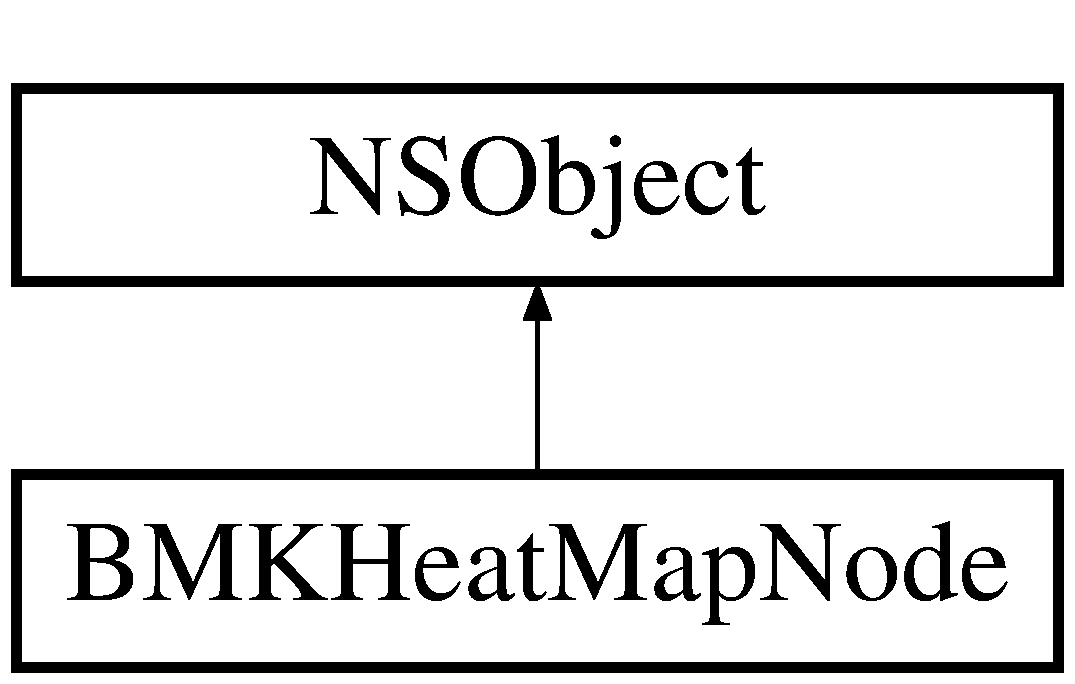
\includegraphics[height=2.000000cm]{interface_b_m_k_heat_map_node}
\end{center}
\end{figure}
\subsection*{Protected 属性}
\begin{DoxyCompactItemize}
\item 
\hypertarget{interface_b_m_k_heat_map_node_af1afa300b9057a129abdf531405fb4bf}{double {\bfseries \+\_\+intensity}}\label{interface_b_m_k_heat_map_node_af1afa300b9057a129abdf531405fb4bf}

\item 
\hypertarget{interface_b_m_k_heat_map_node_a52a3c9cf57869c93e99aae094f44edec}{C\+L\+Location\+Coordinate2\+D {\bfseries \+\_\+pt}}\label{interface_b_m_k_heat_map_node_a52a3c9cf57869c93e99aae094f44edec}

\end{DoxyCompactItemize}
\subsection*{属性}
\begin{DoxyCompactItemize}
\item 
\hypertarget{interface_b_m_k_heat_map_node_ac1ab14f83204a0e5f4a16180acc30742}{double \hyperlink{interface_b_m_k_heat_map_node_ac1ab14f83204a0e5f4a16180acc30742}{intensity}}\label{interface_b_m_k_heat_map_node_ac1ab14f83204a0e5f4a16180acc30742}

\begin{DoxyCompactList}\small\item\em 点的强度权值 \end{DoxyCompactList}\item 
\hypertarget{interface_b_m_k_heat_map_node_a7dcd370e65e376d8253e9a9d127dc984}{C\+L\+Location\+Coordinate2\+D \hyperlink{interface_b_m_k_heat_map_node_a7dcd370e65e376d8253e9a9d127dc984}{pt}}\label{interface_b_m_k_heat_map_node_a7dcd370e65e376d8253e9a9d127dc984}

\begin{DoxyCompactList}\small\item\em 点的位置坐标 \end{DoxyCompactList}\end{DoxyCompactItemize}


\subsection{详细描述}
热力图节点信息 

该类的文档由以下文件生成\+:\begin{DoxyCompactItemize}
\item 
output/map\+\_\+search\+\_\+cloud\+\_\+loc\+\_\+util/inc/B\+M\+K\+Heat\+Map.\+h\end{DoxyCompactItemize}

\hypertarget{interface_b_m_k_location_service}{\section{B\+M\+K\+Location\+Service类 参考}
\label{interface_b_m_k_location_service}\index{B\+M\+K\+Location\+Service@{B\+M\+K\+Location\+Service}}
}
类 B\+M\+K\+Location\+Service 继承关系图\+:\begin{figure}[H]
\begin{center}
\leavevmode
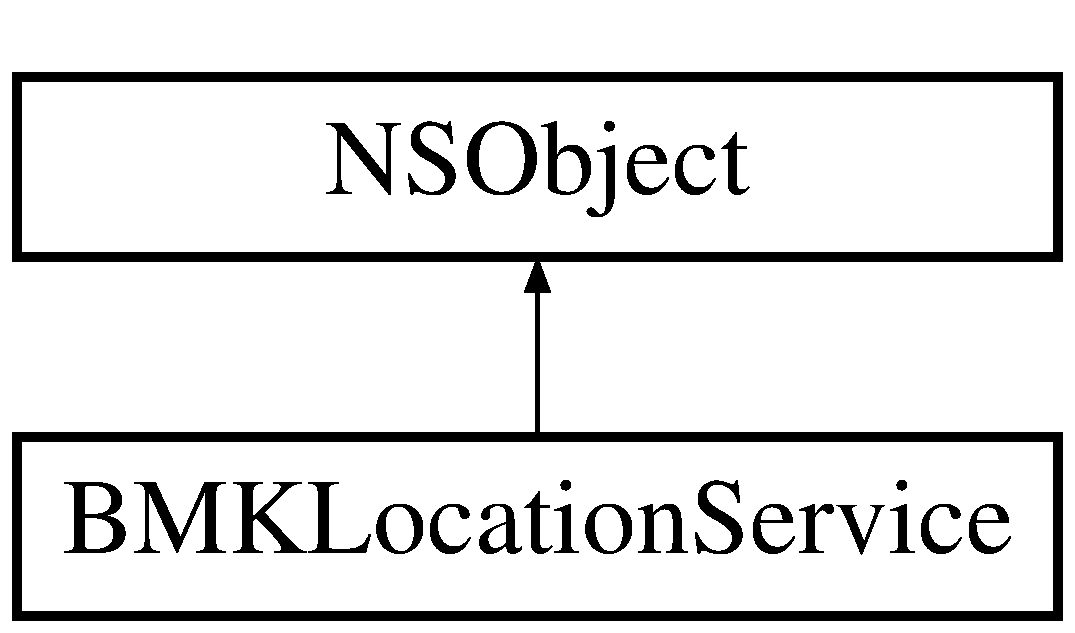
\includegraphics[height=2.000000cm]{interface_b_m_k_location_service}
\end{center}
\end{figure}
\subsection*{Instance Methods}
\begin{DoxyCompactItemize}
\item 
(void) -\/ \hyperlink{interface_b_m_k_location_service_a3b49abd4104d23a114b7a7a632ff3722}{start\+User\+Location\+Service}
\item 
(void) -\/ \hyperlink{interface_b_m_k_location_service_a1aece8fbe579debdd0984147e036e947}{stop\+User\+Location\+Service}
\end{DoxyCompactItemize}
\subsection*{Class Methods}
\begin{DoxyCompactItemize}
\item 
\hypertarget{interface_b_m_k_location_service_abc5a09b7684f33dba3b9863a8e279d9d}{(void) + {\bfseries set\+Location\+Distance\+Filter\+:}}\label{interface_b_m_k_location_service_abc5a09b7684f33dba3b9863a8e279d9d}

\item 
\hypertarget{interface_b_m_k_location_service_a7bedc55fa842dc67e5e6e332de2f934e}{(C\+L\+Location\+Distance) + {\bfseries get\+Current\+Location\+Distance\+Filter}}\label{interface_b_m_k_location_service_a7bedc55fa842dc67e5e6e332de2f934e}

\item 
\hypertarget{interface_b_m_k_location_service_aab4e97f6d6d047ef81895a3acff0f5b4}{(void) + {\bfseries set\+Location\+Desired\+Accuracy\+:}}\label{interface_b_m_k_location_service_aab4e97f6d6d047ef81895a3acff0f5b4}

\item 
\hypertarget{interface_b_m_k_location_service_a3b0b3c85476716fbbea4a535e38e038c}{(C\+L\+Location\+Accuracy) + {\bfseries get\+Current\+Location\+Desired\+Accuracy}}\label{interface_b_m_k_location_service_a3b0b3c85476716fbbea4a535e38e038c}

\end{DoxyCompactItemize}
\subsection*{属性}
\begin{DoxyCompactItemize}
\item 
\hypertarget{interface_b_m_k_location_service_a19c6477dc79e94c8e20d7ddf1e52b0c2}{\hyperlink{interface_b_m_k_user_location}{B\+M\+K\+User\+Location} $\ast$ \hyperlink{interface_b_m_k_location_service_a19c6477dc79e94c8e20d7ddf1e52b0c2}{user\+Location}}\label{interface_b_m_k_location_service_a19c6477dc79e94c8e20d7ddf1e52b0c2}

\begin{DoxyCompactList}\small\item\em 当前用户位置,返回坐标为百度坐标 \end{DoxyCompactList}\item 
\hypertarget{interface_b_m_k_location_service_a6a3767cb278c4dba0a59950586b5e37d}{id$<$ \hyperlink{protocol_b_m_k_location_service_delegate-p}{B\+M\+K\+Location\+Service\+Delegate} $>$ \hyperlink{interface_b_m_k_location_service_a6a3767cb278c4dba0a59950586b5e37d}{delegate}}\label{interface_b_m_k_location_service_a6a3767cb278c4dba0a59950586b5e37d}

\begin{DoxyCompactList}\small\item\em 定位服务\+Delegate,调用start\+User\+Location\+Service定位成功后,用此\+Delegate来获取定位数据 \end{DoxyCompactList}\end{DoxyCompactItemize}


\subsection{Method Documentation}
\hypertarget{interface_b_m_k_location_service_a3b49abd4104d23a114b7a7a632ff3722}{\index{B\+M\+K\+Location\+Service@{B\+M\+K\+Location\+Service}!start\+User\+Location\+Service@{start\+User\+Location\+Service}}
\index{start\+User\+Location\+Service@{start\+User\+Location\+Service}!B\+M\+K\+Location\+Service@{B\+M\+K\+Location\+Service}}
\subsubsection[{start\+User\+Location\+Service}]{\setlength{\rightskip}{0pt plus 5cm}-\/ (void) start\+User\+Location\+Service 
\begin{DoxyParamCaption}
{}
\end{DoxyParamCaption}
}}\label{interface_b_m_k_location_service_a3b49abd4104d23a114b7a7a632ff3722}
打开定位服务 需要在info.\+plist文件中添加(以下二选一,两个都添加默认使用\+N\+S\+Location\+When\+In\+Use\+Usage\+Description): N\+S\+Location\+When\+In\+Use\+Usage\+Description 允许在前台使用时获取\+G\+P\+S的描述 N\+S\+Location\+Always\+Usage\+Description 允许永远可获取\+G\+P\+S的描述 \hypertarget{interface_b_m_k_location_service_a1aece8fbe579debdd0984147e036e947}{\index{B\+M\+K\+Location\+Service@{B\+M\+K\+Location\+Service}!stop\+User\+Location\+Service@{stop\+User\+Location\+Service}}
\index{stop\+User\+Location\+Service@{stop\+User\+Location\+Service}!B\+M\+K\+Location\+Service@{B\+M\+K\+Location\+Service}}
\subsubsection[{stop\+User\+Location\+Service}]{\setlength{\rightskip}{0pt plus 5cm}-\/ (void) stop\+User\+Location\+Service 
\begin{DoxyParamCaption}
{}
\end{DoxyParamCaption}
}}\label{interface_b_m_k_location_service_a1aece8fbe579debdd0984147e036e947}
关闭定位服务 

该类的文档由以下文件生成\+:\begin{DoxyCompactItemize}
\item 
output/map\+\_\+search\+\_\+cloud\+\_\+loc\+\_\+util/inc/B\+M\+K\+Location\+Service.\+h\end{DoxyCompactItemize}

\hypertarget{protocol_b_m_k_location_service_delegate-p}{\section{$<$B\+M\+K\+Location\+Service\+Delegate$>$协议 参考}
\label{protocol_b_m_k_location_service_delegate-p}\index{$<$\+B\+M\+K\+Location\+Service\+Delegate$>$@{$<$\+B\+M\+K\+Location\+Service\+Delegate$>$}}
}


定位服务\+Delegate,调用start\+User\+Location\+Service定位成功后,用此\+Delegate来获取定位数据  




{\ttfamily \#import $<$B\+M\+K\+Location\+Service.\+h$>$}

类 $<$B\+M\+K\+Location\+Service\+Delegate$>$ 继承关系图\+:\begin{figure}[H]
\begin{center}
\leavevmode
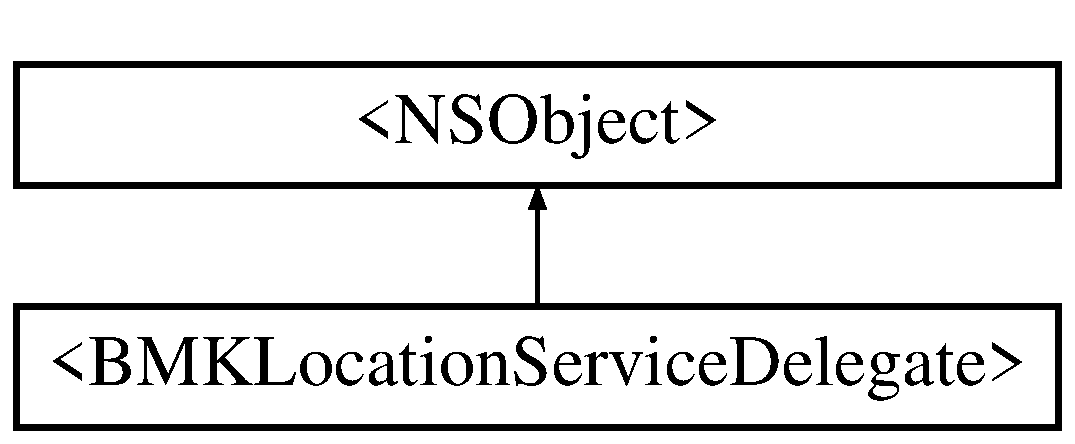
\includegraphics[height=2.000000cm]{protocol_b_m_k_location_service_delegate-p}
\end{center}
\end{figure}
\subsection*{Instance Methods}
\begin{DoxyCompactItemize}
\item 
(void) -\/ \hyperlink{protocol_b_m_k_location_service_delegate-p_a787a16ba232723b8c9594b468ce6714c}{will\+Start\+Locating\+User}
\item 
(void) -\/ \hyperlink{protocol_b_m_k_location_service_delegate-p_a03d0086502462319e2a007b837dc7e26}{did\+Stop\+Locating\+User}
\item 
(void) -\/ \hyperlink{protocol_b_m_k_location_service_delegate-p_a93b210b6948016039b9286cdb350cf13}{did\+Update\+User\+Heading\+:}
\item 
(void) -\/ \hyperlink{protocol_b_m_k_location_service_delegate-p_a3e9ba0b7fca0295aa46a2ad5a179645d}{did\+Update\+B\+M\+K\+User\+Location\+:}
\item 
(void) -\/ \hyperlink{protocol_b_m_k_location_service_delegate-p_a8653218e26f920bf67513c2c4fffb5be}{did\+Fail\+To\+Locate\+User\+With\+Error\+:}
\end{DoxyCompactItemize}


\subsection{详细描述}
定位服务\+Delegate,调用start\+User\+Location\+Service定位成功后,用此\+Delegate来获取定位数据 

\subsection{Method Documentation}
\hypertarget{protocol_b_m_k_location_service_delegate-p_a8653218e26f920bf67513c2c4fffb5be}{\index{B\+M\+K\+Location\+Service\+Delegate-\/p@{B\+M\+K\+Location\+Service\+Delegate-\/p}!did\+Fail\+To\+Locate\+User\+With\+Error\+:@{did\+Fail\+To\+Locate\+User\+With\+Error\+:}}
\index{did\+Fail\+To\+Locate\+User\+With\+Error\+:@{did\+Fail\+To\+Locate\+User\+With\+Error\+:}!B\+M\+K\+Location\+Service\+Delegate-\/p@{B\+M\+K\+Location\+Service\+Delegate-\/p}}
\subsubsection[{did\+Fail\+To\+Locate\+User\+With\+Error\+:}]{\setlength{\rightskip}{0pt plus 5cm}-\/ (void) did\+Fail\+To\+Locate\+User\+With\+Error\+: 
\begin{DoxyParamCaption}
\item[{(N\+S\+Error $\ast$)}]{error}
\end{DoxyParamCaption}
\hspace{0.3cm}{\ttfamily [optional]}}}\label{protocol_b_m_k_location_service_delegate-p_a8653218e26f920bf67513c2c4fffb5be}
定位失败后,会调用此函数 
\begin{DoxyParams}{参数}
{\em error} & 错误号 \\
\hline
\end{DoxyParams}
\hypertarget{protocol_b_m_k_location_service_delegate-p_a03d0086502462319e2a007b837dc7e26}{\index{B\+M\+K\+Location\+Service\+Delegate-\/p@{B\+M\+K\+Location\+Service\+Delegate-\/p}!did\+Stop\+Locating\+User@{did\+Stop\+Locating\+User}}
\index{did\+Stop\+Locating\+User@{did\+Stop\+Locating\+User}!B\+M\+K\+Location\+Service\+Delegate-\/p@{B\+M\+K\+Location\+Service\+Delegate-\/p}}
\subsubsection[{did\+Stop\+Locating\+User}]{\setlength{\rightskip}{0pt plus 5cm}-\/ (void) did\+Stop\+Locating\+User 
\begin{DoxyParamCaption}
{}
\end{DoxyParamCaption}
\hspace{0.3cm}{\ttfamily [optional]}}}\label{protocol_b_m_k_location_service_delegate-p_a03d0086502462319e2a007b837dc7e26}
在停止定位后,会调用此函数 \hypertarget{protocol_b_m_k_location_service_delegate-p_a3e9ba0b7fca0295aa46a2ad5a179645d}{\index{B\+M\+K\+Location\+Service\+Delegate-\/p@{B\+M\+K\+Location\+Service\+Delegate-\/p}!did\+Update\+B\+M\+K\+User\+Location\+:@{did\+Update\+B\+M\+K\+User\+Location\+:}}
\index{did\+Update\+B\+M\+K\+User\+Location\+:@{did\+Update\+B\+M\+K\+User\+Location\+:}!B\+M\+K\+Location\+Service\+Delegate-\/p@{B\+M\+K\+Location\+Service\+Delegate-\/p}}
\subsubsection[{did\+Update\+B\+M\+K\+User\+Location\+:}]{\setlength{\rightskip}{0pt plus 5cm}-\/ (void) did\+Update\+B\+M\+K\+User\+Location\+: 
\begin{DoxyParamCaption}
\item[{({\bf B\+M\+K\+User\+Location} $\ast$)}]{user\+Location}
\end{DoxyParamCaption}
\hspace{0.3cm}{\ttfamily [optional]}}}\label{protocol_b_m_k_location_service_delegate-p_a3e9ba0b7fca0295aa46a2ad5a179645d}
用户位置更新后,会调用此函数 
\begin{DoxyParams}{参数}
{\em user\+Location} & 新的用户位置 \\
\hline
\end{DoxyParams}
\hypertarget{protocol_b_m_k_location_service_delegate-p_a93b210b6948016039b9286cdb350cf13}{\index{B\+M\+K\+Location\+Service\+Delegate-\/p@{B\+M\+K\+Location\+Service\+Delegate-\/p}!did\+Update\+User\+Heading\+:@{did\+Update\+User\+Heading\+:}}
\index{did\+Update\+User\+Heading\+:@{did\+Update\+User\+Heading\+:}!B\+M\+K\+Location\+Service\+Delegate-\/p@{B\+M\+K\+Location\+Service\+Delegate-\/p}}
\subsubsection[{did\+Update\+User\+Heading\+:}]{\setlength{\rightskip}{0pt plus 5cm}-\/ (void) did\+Update\+User\+Heading\+: 
\begin{DoxyParamCaption}
\item[{({\bf B\+M\+K\+User\+Location} $\ast$)}]{user\+Location}
\end{DoxyParamCaption}
\hspace{0.3cm}{\ttfamily [optional]}}}\label{protocol_b_m_k_location_service_delegate-p_a93b210b6948016039b9286cdb350cf13}
用户方向更新后,会调用此函数 
\begin{DoxyParams}{参数}
{\em user\+Location} & 新的用户位置 \\
\hline
\end{DoxyParams}
\hypertarget{protocol_b_m_k_location_service_delegate-p_a787a16ba232723b8c9594b468ce6714c}{\index{B\+M\+K\+Location\+Service\+Delegate-\/p@{B\+M\+K\+Location\+Service\+Delegate-\/p}!will\+Start\+Locating\+User@{will\+Start\+Locating\+User}}
\index{will\+Start\+Locating\+User@{will\+Start\+Locating\+User}!B\+M\+K\+Location\+Service\+Delegate-\/p@{B\+M\+K\+Location\+Service\+Delegate-\/p}}
\subsubsection[{will\+Start\+Locating\+User}]{\setlength{\rightskip}{0pt plus 5cm}-\/ (void) will\+Start\+Locating\+User 
\begin{DoxyParamCaption}
{}
\end{DoxyParamCaption}
\hspace{0.3cm}{\ttfamily [optional]}}}\label{protocol_b_m_k_location_service_delegate-p_a787a16ba232723b8c9594b468ce6714c}
在将要启动定位时,会调用此函数 

该协议的文档由以下文件生成\+:\begin{DoxyCompactItemize}
\item 
output/map\+\_\+search\+\_\+cloud\+\_\+loc\+\_\+util/inc/B\+M\+K\+Location\+Service.\+h\end{DoxyCompactItemize}

\hypertarget{interface_b_m_k_location_share_u_r_l_option}{\section{B\+M\+K\+Location\+Share\+U\+R\+L\+Option类 参考}
\label{interface_b_m_k_location_share_u_r_l_option}\index{B\+M\+K\+Location\+Share\+U\+R\+L\+Option@{B\+M\+K\+Location\+Share\+U\+R\+L\+Option}}
}


反geo短串分享检索信息类  




{\ttfamily \#import $<$B\+M\+K\+Share\+Url\+Search\+Option.\+h$>$}

类 B\+M\+K\+Location\+Share\+U\+R\+L\+Option 继承关系图\+:\begin{figure}[H]
\begin{center}
\leavevmode
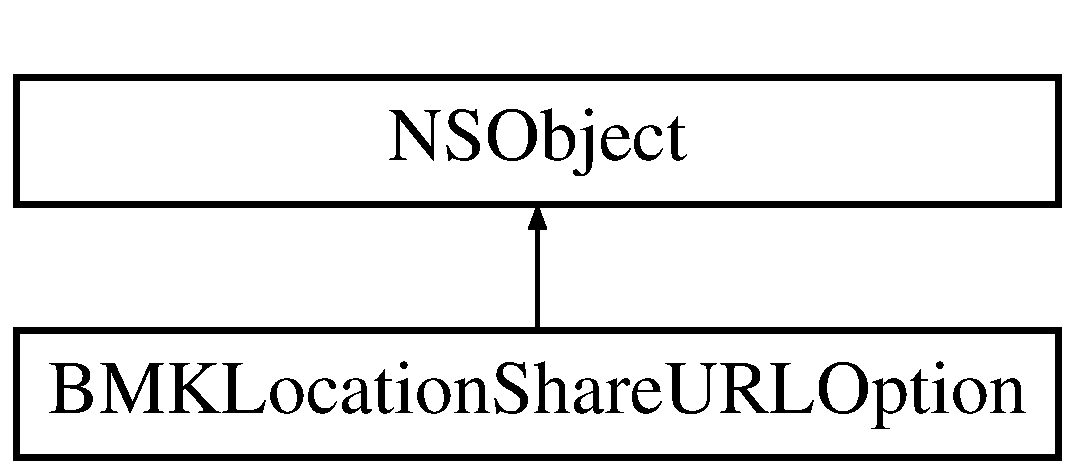
\includegraphics[height=2.000000cm]{interface_b_m_k_location_share_u_r_l_option}
\end{center}
\end{figure}
\subsection*{Protected 属性}
\begin{DoxyCompactItemize}
\item 
\hypertarget{interface_b_m_k_location_share_u_r_l_option_aa7590ba3b21f55434f5854778974b9c4}{N\+S\+String $\ast$ {\bfseries \+\_\+name}}\label{interface_b_m_k_location_share_u_r_l_option_aa7590ba3b21f55434f5854778974b9c4}

\item 
\hypertarget{interface_b_m_k_location_share_u_r_l_option_a455c7467cf0814dbe3219e7ed596b38a}{N\+S\+String $\ast$ {\bfseries \+\_\+snippet}}\label{interface_b_m_k_location_share_u_r_l_option_a455c7467cf0814dbe3219e7ed596b38a}

\item 
\hypertarget{interface_b_m_k_location_share_u_r_l_option_a67aa843182abf143e68a89d9fbe3441c}{C\+L\+Location\+Coordinate2\+D {\bfseries \+\_\+location}}\label{interface_b_m_k_location_share_u_r_l_option_a67aa843182abf143e68a89d9fbe3441c}

\end{DoxyCompactItemize}
\subsection*{属性}
\begin{DoxyCompactItemize}
\item 
\hypertarget{interface_b_m_k_location_share_u_r_l_option_a11f562286c830a4e78f9c7f1d40aded4}{N\+S\+String $\ast$ \hyperlink{interface_b_m_k_location_share_u_r_l_option_a11f562286c830a4e78f9c7f1d40aded4}{name}}\label{interface_b_m_k_location_share_u_r_l_option_a11f562286c830a4e78f9c7f1d40aded4}

\begin{DoxyCompactList}\small\item\em 名称 \end{DoxyCompactList}\item 
\hypertarget{interface_b_m_k_location_share_u_r_l_option_a9eb77e28dac4084933eb17cd3adef344}{N\+S\+String $\ast$ \hyperlink{interface_b_m_k_location_share_u_r_l_option_a9eb77e28dac4084933eb17cd3adef344}{snippet}}\label{interface_b_m_k_location_share_u_r_l_option_a9eb77e28dac4084933eb17cd3adef344}

\begin{DoxyCompactList}\small\item\em 通过短\+U\+R\+L调起客户端时作为附加信息显示在名称下面 \end{DoxyCompactList}\item 
\hypertarget{interface_b_m_k_location_share_u_r_l_option_adecb9b65fe164ed23f271b0693bfa354}{C\+L\+Location\+Coordinate2\+D \hyperlink{interface_b_m_k_location_share_u_r_l_option_adecb9b65fe164ed23f271b0693bfa354}{location}}\label{interface_b_m_k_location_share_u_r_l_option_adecb9b65fe164ed23f271b0693bfa354}

\begin{DoxyCompactList}\small\item\em 经纬度 \end{DoxyCompactList}\end{DoxyCompactItemize}


\subsection{详细描述}
反geo短串分享检索信息类 

该类的文档由以下文件生成\+:\begin{DoxyCompactItemize}
\item 
output/map\+\_\+search\+\_\+cloud\+\_\+loc\+\_\+util/inc/B\+M\+K\+Share\+Url\+Search\+Option.\+h\end{DoxyCompactItemize}

\hypertarget{interface_b_m_k_location_view_display_param}{\section{B\+M\+K\+Location\+View\+Display\+Param类 参考}
\label{interface_b_m_k_location_view_display_param}\index{B\+M\+K\+Location\+View\+Display\+Param@{B\+M\+K\+Location\+View\+Display\+Param}}
}


此类表示定位图层自定义样式参数  




{\ttfamily \#import $<$B\+M\+K\+Location\+View\+Display\+Param.\+h$>$}

类 B\+M\+K\+Location\+View\+Display\+Param 继承关系图\+:\begin{figure}[H]
\begin{center}
\leavevmode
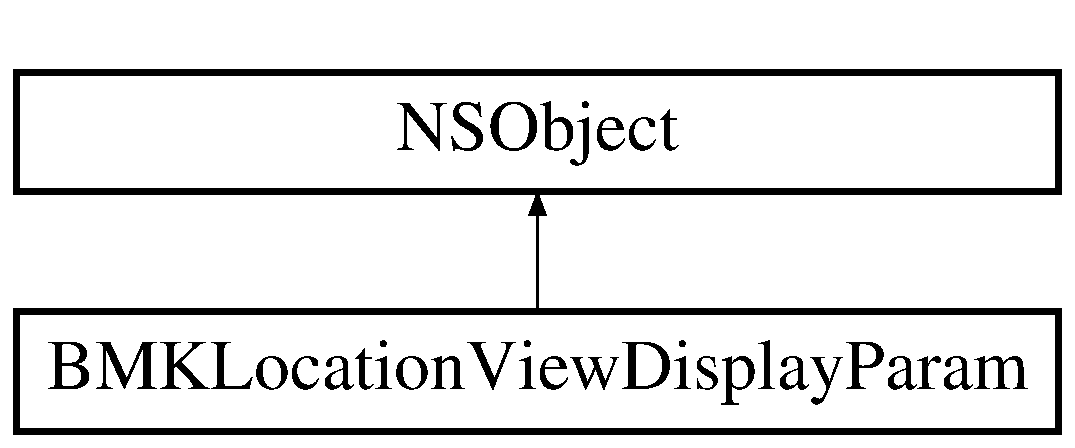
\includegraphics[height=2.000000cm]{interface_b_m_k_location_view_display_param}
\end{center}
\end{figure}
\subsection*{Protected 属性}
\begin{DoxyCompactItemize}
\item 
\hypertarget{interface_b_m_k_location_view_display_param_aca7d451721e1c1e3f75766fe3a3572e1}{float {\bfseries \+\_\+location\+View\+Offset\+X}}\label{interface_b_m_k_location_view_display_param_aca7d451721e1c1e3f75766fe3a3572e1}

\item 
\hypertarget{interface_b_m_k_location_view_display_param_a7914b096cec7ba724e9eb0b752c77dc0}{float {\bfseries \+\_\+location\+View\+Offset\+Y}}\label{interface_b_m_k_location_view_display_param_a7914b096cec7ba724e9eb0b752c77dc0}

\item 
\hypertarget{interface_b_m_k_location_view_display_param_a376ad9f3e561b1ff5c1fed963ffa62b8}{bool {\bfseries \+\_\+is\+Accuracy\+Circle\+Show}}\label{interface_b_m_k_location_view_display_param_a376ad9f3e561b1ff5c1fed963ffa62b8}

\item 
\hypertarget{interface_b_m_k_location_view_display_param_a9a113a1e0217f64e06311e752263d6e0}{bool {\bfseries \+\_\+is\+Rotate\+Angle\+Valid}}\label{interface_b_m_k_location_view_display_param_a9a113a1e0217f64e06311e752263d6e0}

\item 
\hypertarget{interface_b_m_k_location_view_display_param_a8cc611777402a8a9ca0fe3b12a48d87b}{N\+S\+String $\ast$ {\bfseries \+\_\+location\+View\+Img\+Name}}\label{interface_b_m_k_location_view_display_param_a8cc611777402a8a9ca0fe3b12a48d87b}

\end{DoxyCompactItemize}
\subsection*{属性}
\begin{DoxyCompactItemize}
\item 
\hypertarget{interface_b_m_k_location_view_display_param_a7b5ee93aed161a1d0456d83627b558df}{float \hyperlink{interface_b_m_k_location_view_display_param_a7b5ee93aed161a1d0456d83627b558df}{location\+View\+Offset\+X}}\label{interface_b_m_k_location_view_display_param_a7b5ee93aed161a1d0456d83627b558df}

\begin{DoxyCompactList}\small\item\em 定位图标偏移量\+X \end{DoxyCompactList}\item 
\hypertarget{interface_b_m_k_location_view_display_param_a187fc86fdc3a3630a59f1f1e22815085}{float \hyperlink{interface_b_m_k_location_view_display_param_a187fc86fdc3a3630a59f1f1e22815085}{location\+View\+Offset\+Y}}\label{interface_b_m_k_location_view_display_param_a187fc86fdc3a3630a59f1f1e22815085}

\begin{DoxyCompactList}\small\item\em 定位图标偏移量\+Y \end{DoxyCompactList}\item 
\hypertarget{interface_b_m_k_location_view_display_param_acf79f27e03fd92e8594ccd66a6e332b5}{bool \hyperlink{interface_b_m_k_location_view_display_param_acf79f27e03fd92e8594ccd66a6e332b5}{is\+Accuracy\+Circle\+Show}}\label{interface_b_m_k_location_view_display_param_acf79f27e03fd92e8594ccd66a6e332b5}

\begin{DoxyCompactList}\small\item\em 精度圈是否显示 \end{DoxyCompactList}\item 
\hypertarget{interface_b_m_k_location_view_display_param_a7e6cdb5311a7b6292a4c5f454975e840}{bool \hyperlink{interface_b_m_k_location_view_display_param_a7e6cdb5311a7b6292a4c5f454975e840}{is\+Rotate\+Angle\+Valid}}\label{interface_b_m_k_location_view_display_param_a7e6cdb5311a7b6292a4c5f454975e840}

\begin{DoxyCompactList}\small\item\em 跟随态旋转角度是否生效 \end{DoxyCompactList}\item 
\hypertarget{interface_b_m_k_location_view_display_param_af122b975fe0c3d636b94226382475366}{N\+S\+String $\ast$ \hyperlink{interface_b_m_k_location_view_display_param_af122b975fe0c3d636b94226382475366}{location\+View\+Img\+Name}}\label{interface_b_m_k_location_view_display_param_af122b975fe0c3d636b94226382475366}

\begin{DoxyCompactList}\small\item\em 定位图标 \end{DoxyCompactList}\end{DoxyCompactItemize}


\subsection{详细描述}
此类表示定位图层自定义样式参数 

该类的文档由以下文件生成\+:\begin{DoxyCompactItemize}
\item 
output/map\+\_\+search\+\_\+cloud\+\_\+loc\+\_\+util/inc/B\+M\+K\+Location\+View\+Display\+Param.\+h\end{DoxyCompactItemize}

\hypertarget{interface_b_m_k_map_manager}{\section{B\+M\+K\+Map\+Manager类 参考}
\label{interface_b_m_k_map_manager}\index{B\+M\+K\+Map\+Manager@{B\+M\+K\+Map\+Manager}}
}


主引擎类  




{\ttfamily \#import $<$B\+M\+K\+Map\+Manager.\+h$>$}

类 B\+M\+K\+Map\+Manager 继承关系图\+:\begin{figure}[H]
\begin{center}
\leavevmode
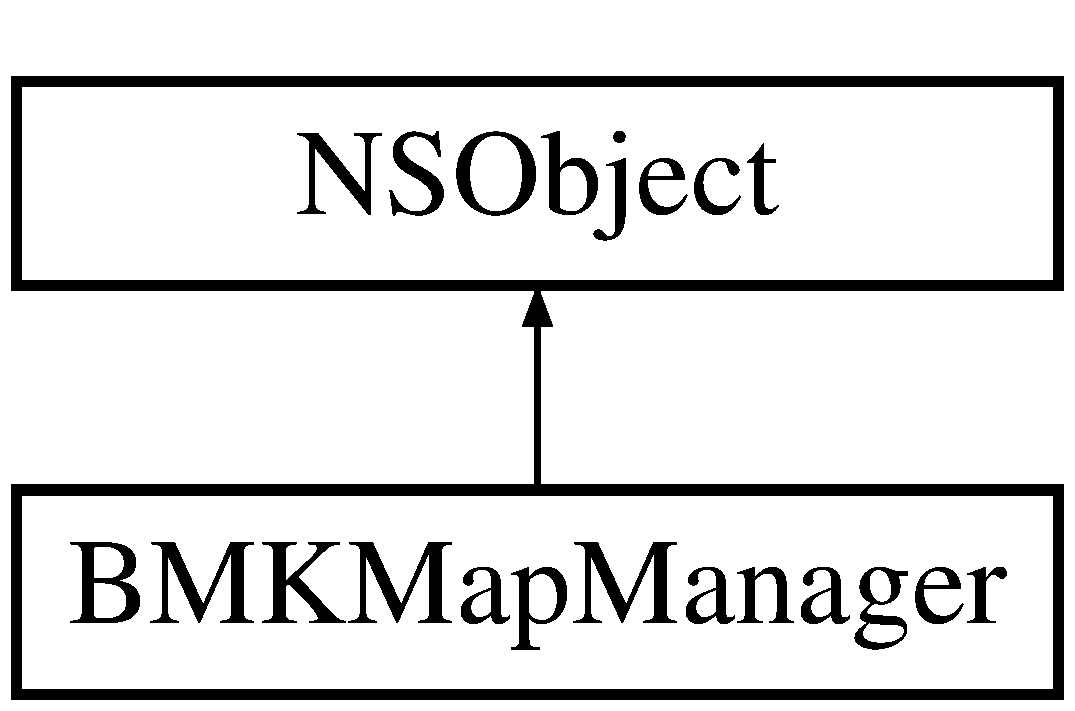
\includegraphics[height=2.000000cm]{interface_b_m_k_map_manager}
\end{center}
\end{figure}
\subsection*{Instance Methods}
\begin{DoxyCompactItemize}
\item 
(B\+O\+O\+L) -\/ \hyperlink{interface_b_m_k_map_manager_a95edf9c8fea4c61a79098641c4e9a50f}{start\+:general\+Delegate\+:}
\item 
(B\+O\+O\+L) -\/ \hyperlink{interface_b_m_k_map_manager_ac53850202f5017ff35c8933c171be0f1}{stop}
\end{DoxyCompactItemize}


\subsection{详细描述}
主引擎类 

\subsection{Method Documentation}
\hypertarget{interface_b_m_k_map_manager_a95edf9c8fea4c61a79098641c4e9a50f}{\index{B\+M\+K\+Map\+Manager@{B\+M\+K\+Map\+Manager}!start\+:general\+Delegate\+:@{start\+:general\+Delegate\+:}}
\index{start\+:general\+Delegate\+:@{start\+:general\+Delegate\+:}!B\+M\+K\+Map\+Manager@{B\+M\+K\+Map\+Manager}}
\subsubsection[{start\+:general\+Delegate\+:}]{\setlength{\rightskip}{0pt plus 5cm}-\/ (B\+O\+O\+L) start\+: 
\begin{DoxyParamCaption}
\item[{(N\+S\+String $\ast$)}]{key}
\item[{generalDelegate:(id$<$ {\bf B\+M\+K\+General\+Delegate} $>$)}]{delegate}
\end{DoxyParamCaption}
}}\label{interface_b_m_k_map_manager_a95edf9c8fea4c61a79098641c4e9a50f}
启动引擎 
\begin{DoxyParams}{参数}
{\em key} & 申请的有效key \\
\hline
{\em delegate} & \\
\hline
\end{DoxyParams}
\hypertarget{interface_b_m_k_map_manager_ac53850202f5017ff35c8933c171be0f1}{\index{B\+M\+K\+Map\+Manager@{B\+M\+K\+Map\+Manager}!stop@{stop}}
\index{stop@{stop}!B\+M\+K\+Map\+Manager@{B\+M\+K\+Map\+Manager}}
\subsubsection[{stop}]{\setlength{\rightskip}{0pt plus 5cm}-\/ (B\+O\+O\+L) stop 
\begin{DoxyParamCaption}
{}
\end{DoxyParamCaption}
}}\label{interface_b_m_k_map_manager_ac53850202f5017ff35c8933c171be0f1}
停止引擎 

该类的文档由以下文件生成\+:\begin{DoxyCompactItemize}
\item 
output/map\+\_\+search\+\_\+cloud\+\_\+loc\+\_\+util/inc/B\+M\+K\+Map\+Manager.\+h\end{DoxyCompactItemize}

\hypertarget{interface_b_m_k_map_poi}{\section{B\+M\+K\+Map\+Poi类 参考}
\label{interface_b_m_k_map_poi}\index{B\+M\+K\+Map\+Poi@{B\+M\+K\+Map\+Poi}}
}


点击地图标注返回数据结构  




{\ttfamily \#import $<$B\+M\+K\+Map\+View.\+h$>$}

类 B\+M\+K\+Map\+Poi 继承关系图\+:\begin{figure}[H]
\begin{center}
\leavevmode
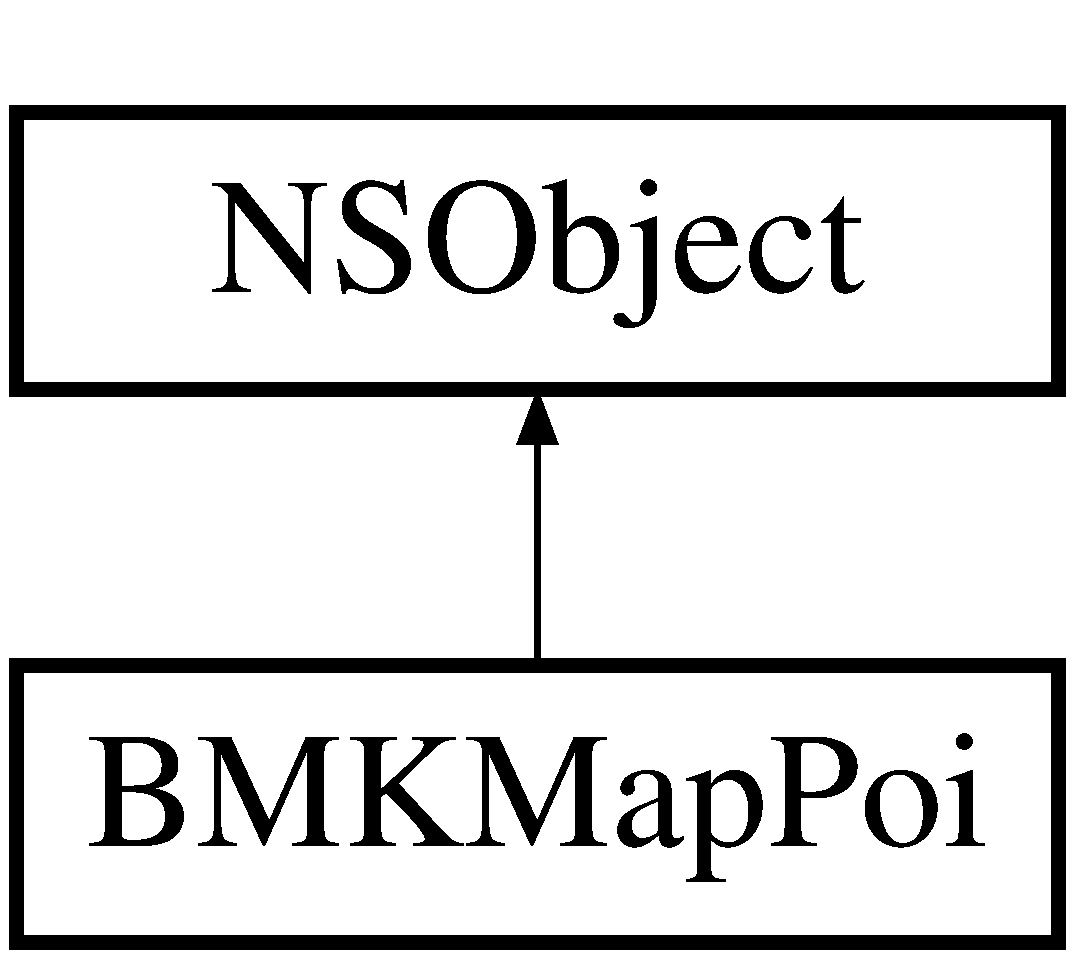
\includegraphics[height=2.000000cm]{interface_b_m_k_map_poi}
\end{center}
\end{figure}
\subsection*{属性}
\begin{DoxyCompactItemize}
\item 
\hypertarget{interface_b_m_k_map_poi_a5d5c19bd352dcab43167d97aa47ea38d}{N\+S\+String $\ast$ \hyperlink{interface_b_m_k_map_poi_a5d5c19bd352dcab43167d97aa47ea38d}{text}}\label{interface_b_m_k_map_poi_a5d5c19bd352dcab43167d97aa47ea38d}

\begin{DoxyCompactList}\small\item\em 点标注的名称 \end{DoxyCompactList}\item 
\hypertarget{interface_b_m_k_map_poi_a771c0672bbe2dd1dc526003717bbcec1}{C\+L\+Location\+Coordinate2\+D \hyperlink{interface_b_m_k_map_poi_a771c0672bbe2dd1dc526003717bbcec1}{pt}}\label{interface_b_m_k_map_poi_a771c0672bbe2dd1dc526003717bbcec1}

\begin{DoxyCompactList}\small\item\em 点标注的经纬度坐标 \end{DoxyCompactList}\end{DoxyCompactItemize}


\subsection{详细描述}
点击地图标注返回数据结构 

该类的文档由以下文件生成\+:\begin{DoxyCompactItemize}
\item 
output/map\+\_\+search\+\_\+cloud\+\_\+loc\+\_\+util/inc/B\+M\+K\+Map\+View.\+h\end{DoxyCompactItemize}

\hypertarget{struct_b_m_k_map_point}{\section{B\+M\+K\+Map\+Point结构体 参考}
\label{struct_b_m_k_map_point}\index{B\+M\+K\+Map\+Point@{B\+M\+K\+Map\+Point}}
}


地理坐标点,用直角地理坐标表示  




{\ttfamily \#include $<$B\+M\+K\+Types.\+h$>$}

\subsection*{Public 属性}
\begin{DoxyCompactItemize}
\item 
\hypertarget{struct_b_m_k_map_point_a8c0ca1c3f0cbb5fe183ae7745781d8fb}{double \hyperlink{struct_b_m_k_map_point_a8c0ca1c3f0cbb5fe183ae7745781d8fb}{x}}\label{struct_b_m_k_map_point_a8c0ca1c3f0cbb5fe183ae7745781d8fb}

\begin{DoxyCompactList}\small\item\em 横坐标 \end{DoxyCompactList}\item 
\hypertarget{struct_b_m_k_map_point_a9d0aff0bad009459af85d1e51a194341}{double \hyperlink{struct_b_m_k_map_point_a9d0aff0bad009459af85d1e51a194341}{y}}\label{struct_b_m_k_map_point_a9d0aff0bad009459af85d1e51a194341}

\begin{DoxyCompactList}\small\item\em 纵坐标 \end{DoxyCompactList}\end{DoxyCompactItemize}


\subsection{详细描述}
地理坐标点,用直角地理坐标表示 

该结构体的文档由以下文件生成\+:\begin{DoxyCompactItemize}
\item 
output/map\+\_\+search\+\_\+cloud\+\_\+loc\+\_\+util/inc/B\+M\+K\+Types.\+h\end{DoxyCompactItemize}

\hypertarget{struct_b_m_k_map_rect}{\section{B\+M\+K\+Map\+Rect结构体 参考}
\label{struct_b_m_k_map_rect}\index{B\+M\+K\+Map\+Rect@{B\+M\+K\+Map\+Rect}}
}


矩形,用直角地理坐标表示  




{\ttfamily \#include $<$B\+M\+K\+Types.\+h$>$}

\subsection*{Public 属性}
\begin{DoxyCompactItemize}
\item 
\hypertarget{struct_b_m_k_map_rect_aeeee8bcaabf5c65e222f1891009325f1}{\hyperlink{struct_b_m_k_map_point}{B\+M\+K\+Map\+Point} \hyperlink{struct_b_m_k_map_rect_aeeee8bcaabf5c65e222f1891009325f1}{origin}}\label{struct_b_m_k_map_rect_aeeee8bcaabf5c65e222f1891009325f1}

\begin{DoxyCompactList}\small\item\em 屏幕左上点对应的直角地理坐标 \end{DoxyCompactList}\item 
\hypertarget{struct_b_m_k_map_rect_ab83b0fb9e6e63b6ab24bdce9ced1e92e}{\hyperlink{struct_b_m_k_map_size}{B\+M\+K\+Map\+Size} \hyperlink{struct_b_m_k_map_rect_ab83b0fb9e6e63b6ab24bdce9ced1e92e}{size}}\label{struct_b_m_k_map_rect_ab83b0fb9e6e63b6ab24bdce9ced1e92e}

\begin{DoxyCompactList}\small\item\em 坐标范围 \end{DoxyCompactList}\end{DoxyCompactItemize}


\subsection{详细描述}
矩形,用直角地理坐标表示 

该结构体的文档由以下文件生成\+:\begin{DoxyCompactItemize}
\item 
output/map\+\_\+search\+\_\+cloud\+\_\+loc\+\_\+util/inc/B\+M\+K\+Types.\+h\end{DoxyCompactItemize}

\hypertarget{struct_b_m_k_map_size}{\section{B\+M\+K\+Map\+Size结构体 参考}
\label{struct_b_m_k_map_size}\index{B\+M\+K\+Map\+Size@{B\+M\+K\+Map\+Size}}
}


矩形大小,用直角地理坐标表示  




{\ttfamily \#include $<$B\+M\+K\+Types.\+h$>$}

\subsection*{Public 属性}
\begin{DoxyCompactItemize}
\item 
\hypertarget{struct_b_m_k_map_size_a1005d7fd59045a80619c024df3156d6a}{double \hyperlink{struct_b_m_k_map_size_a1005d7fd59045a80619c024df3156d6a}{width}}\label{struct_b_m_k_map_size_a1005d7fd59045a80619c024df3156d6a}

\begin{DoxyCompactList}\small\item\em 宽度 \end{DoxyCompactList}\item 
\hypertarget{struct_b_m_k_map_size_a516baff78187bf8f07ef49f01c7d86fc}{double \hyperlink{struct_b_m_k_map_size_a516baff78187bf8f07ef49f01c7d86fc}{height}}\label{struct_b_m_k_map_size_a516baff78187bf8f07ef49f01c7d86fc}

\begin{DoxyCompactList}\small\item\em 高度 \end{DoxyCompactList}\end{DoxyCompactItemize}


\subsection{详细描述}
矩形大小,用直角地理坐标表示 

该结构体的文档由以下文件生成\+:\begin{DoxyCompactItemize}
\item 
output/map\+\_\+search\+\_\+cloud\+\_\+loc\+\_\+util/inc/B\+M\+K\+Types.\+h\end{DoxyCompactItemize}

\hypertarget{interface_b_m_k_map_status}{\section{B\+M\+K\+Map\+Status类 参考}
\label{interface_b_m_k_map_status}\index{B\+M\+K\+Map\+Status@{B\+M\+K\+Map\+Status}}
}


此类表示地图状态信息  




{\ttfamily \#import $<$B\+M\+K\+Map\+Status.\+h$>$}

类 B\+M\+K\+Map\+Status 继承关系图\+:\begin{figure}[H]
\begin{center}
\leavevmode
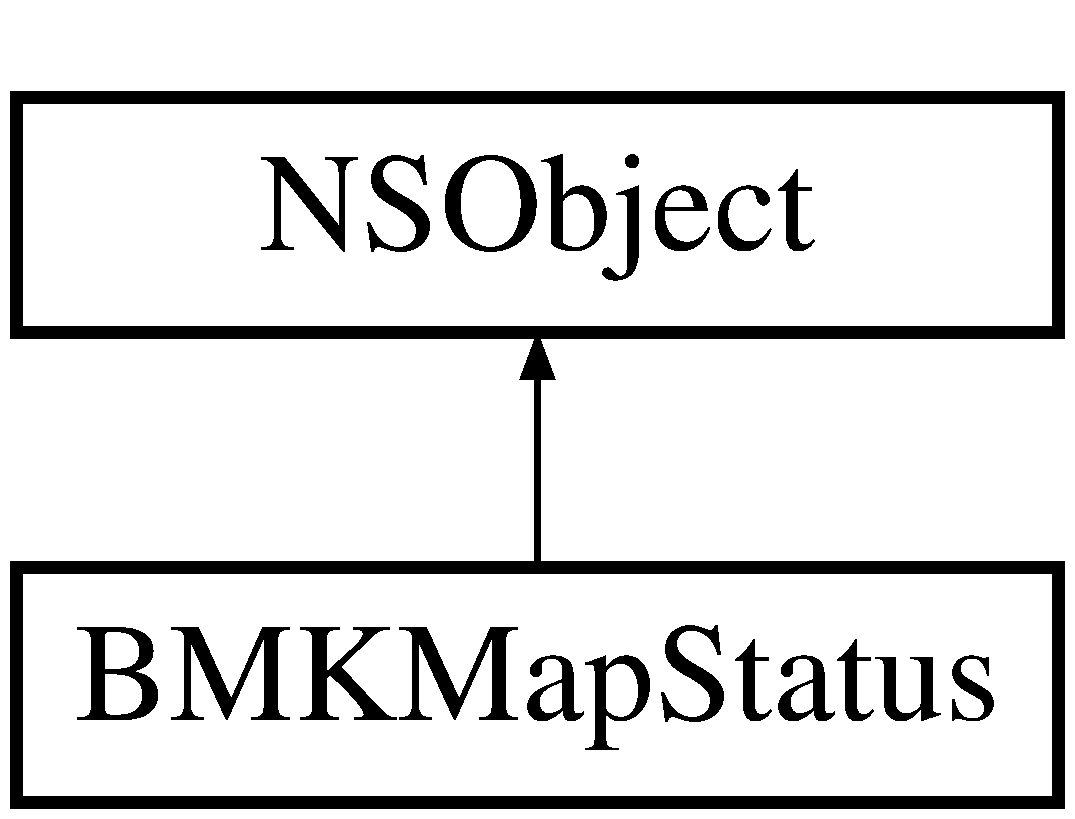
\includegraphics[height=2.000000cm]{interface_b_m_k_map_status}
\end{center}
\end{figure}
\subsection*{Protected 属性}
\begin{DoxyCompactItemize}
\item 
\hypertarget{interface_b_m_k_map_status_a0c67450ec78dc6be5e87fed6aa3ade92}{float {\bfseries \+\_\+f\+Level}}\label{interface_b_m_k_map_status_a0c67450ec78dc6be5e87fed6aa3ade92}

\item 
\hypertarget{interface_b_m_k_map_status_a04fb6a2f91634c82423dcd9bf07efa12}{float {\bfseries \+\_\+f\+Rotation}}\label{interface_b_m_k_map_status_a04fb6a2f91634c82423dcd9bf07efa12}

\item 
\hypertarget{interface_b_m_k_map_status_a3a4fb7039f93b796646d161e4e87ae77}{float {\bfseries \+\_\+f\+Overlooking}}\label{interface_b_m_k_map_status_a3a4fb7039f93b796646d161e4e87ae77}

\item 
\hypertarget{interface_b_m_k_map_status_aa440aec20efe8874977fa9fc18d71604}{C\+G\+Point {\bfseries \+\_\+target\+Screen\+Pt}}\label{interface_b_m_k_map_status_aa440aec20efe8874977fa9fc18d71604}

\item 
\hypertarget{interface_b_m_k_map_status_adca8672a6bea448a9eadcaf65df7eae2}{C\+L\+Location\+Coordinate2\+D {\bfseries \+\_\+target\+Geo\+Pt}}\label{interface_b_m_k_map_status_adca8672a6bea448a9eadcaf65df7eae2}

\end{DoxyCompactItemize}
\subsection*{属性}
\begin{DoxyCompactItemize}
\item 
\hypertarget{interface_b_m_k_map_status_abe3f9d36eee716ca15394aab89e1134c}{float \hyperlink{interface_b_m_k_map_status_abe3f9d36eee716ca15394aab89e1134c}{f\+Level}}\label{interface_b_m_k_map_status_abe3f9d36eee716ca15394aab89e1134c}

\begin{DoxyCompactList}\small\item\em 缩放级别\+:\mbox{[}3$\sim$19\mbox{]} \end{DoxyCompactList}\item 
\hypertarget{interface_b_m_k_map_status_a3c22c82aead710c2dec187ff1d39e370}{float \hyperlink{interface_b_m_k_map_status_a3c22c82aead710c2dec187ff1d39e370}{f\+Rotation}}\label{interface_b_m_k_map_status_a3c22c82aead710c2dec187ff1d39e370}

\begin{DoxyCompactList}\small\item\em 旋转角度 \end{DoxyCompactList}\item 
\hypertarget{interface_b_m_k_map_status_abd88f1cfbe5a8bbf2503c51802bf5c96}{float \hyperlink{interface_b_m_k_map_status_abd88f1cfbe5a8bbf2503c51802bf5c96}{f\+Overlooking}}\label{interface_b_m_k_map_status_abd88f1cfbe5a8bbf2503c51802bf5c96}

\begin{DoxyCompactList}\small\item\em 俯视角度\+:\mbox{[}-\/45$\sim$0\mbox{]} \end{DoxyCompactList}\item 
\hypertarget{interface_b_m_k_map_status_a902555f3b28504a2217443c496edc491}{C\+G\+Point \hyperlink{interface_b_m_k_map_status_a902555f3b28504a2217443c496edc491}{target\+Screen\+Pt}}\label{interface_b_m_k_map_status_a902555f3b28504a2217443c496edc491}

\begin{DoxyCompactList}\small\item\em 屏幕中心点坐标\+:在屏幕内,超过无效 \end{DoxyCompactList}\item 
\hypertarget{interface_b_m_k_map_status_a98d10950c91d08dce079020baafbe10d}{C\+L\+Location\+Coordinate2\+D \hyperlink{interface_b_m_k_map_status_a98d10950c91d08dce079020baafbe10d}{target\+Geo\+Pt}}\label{interface_b_m_k_map_status_a98d10950c91d08dce079020baafbe10d}

\begin{DoxyCompactList}\small\item\em 地理中心点坐标\+:经纬度 \end{DoxyCompactList}\end{DoxyCompactItemize}


\subsection{详细描述}
此类表示地图状态信息 

该类的文档由以下文件生成\+:\begin{DoxyCompactItemize}
\item 
output/map\+\_\+search\+\_\+cloud\+\_\+loc\+\_\+util/inc/B\+M\+K\+Map\+Status.\+h\end{DoxyCompactItemize}

\hypertarget{interface_b_m_k_map_view}{\section{B\+M\+K\+Map\+View类 参考}
\label{interface_b_m_k_map_view}\index{B\+M\+K\+Map\+View@{B\+M\+K\+Map\+View}}
}


地图\+View类,使用此\+View可以显示地图窗口,并且对地图进行相关的操作  




{\ttfamily \#import $<$B\+M\+K\+Map\+View.\+h$>$}

类 B\+M\+K\+Map\+View 继承关系图\+:\begin{figure}[H]
\begin{center}
\leavevmode
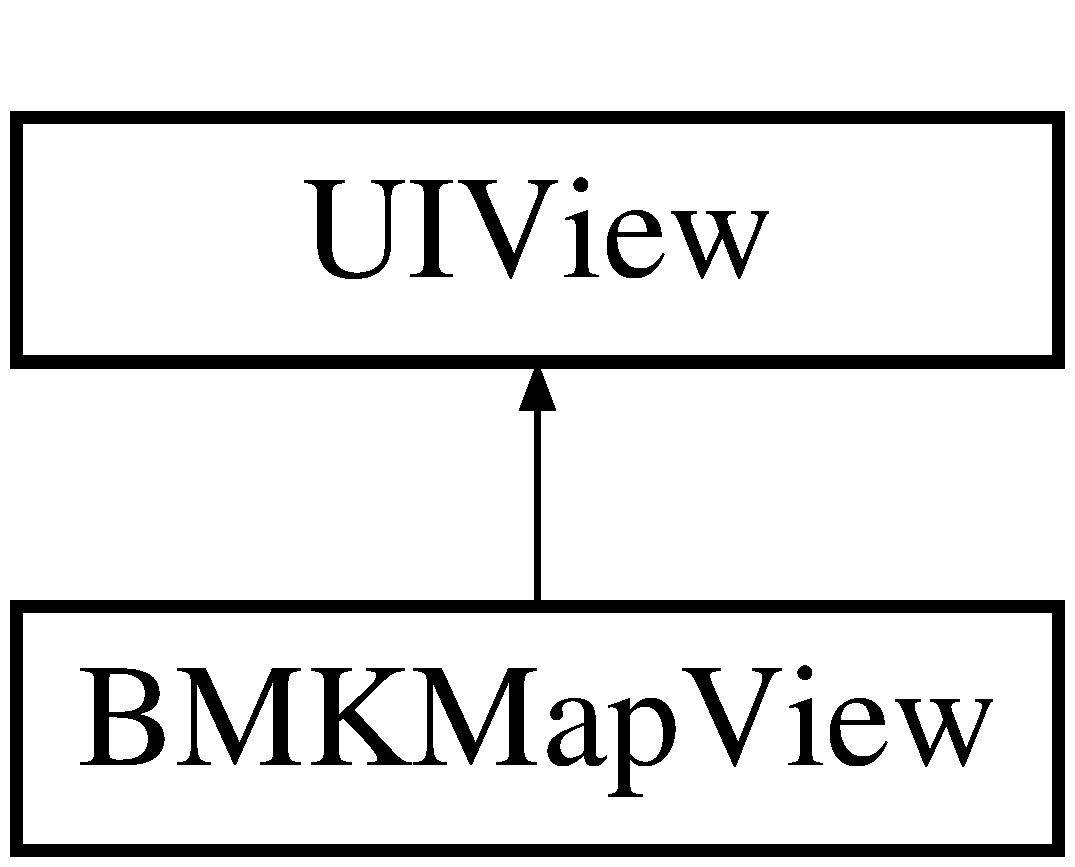
\includegraphics[height=2.000000cm]{interface_b_m_k_map_view}
\end{center}
\end{figure}
\subsection*{Instance Methods}
\begin{DoxyCompactItemize}
\item 
(void) -\/ \hyperlink{interface_b_m_k_map_view_a6ce8ac560bd901b93b3e15d6996a409a}{view\+Will\+Appear}
\item 
(void) -\/ \hyperlink{interface_b_m_k_map_view_a0cfbfc217062e84de41ddb04dcad7e67}{view\+Will\+Disappear}
\item 
(B\+O\+O\+L) -\/ \hyperlink{interface_b_m_k_map_view_a349f7c74871a389d73955edd7bcd9fdf}{zoom\+In}
\item 
(B\+O\+O\+L) -\/ \hyperlink{interface_b_m_k_map_view_a1806c818757917ef674ebe5ba24fe5a2}{zoom\+Out}
\item 
(\hyperlink{struct_b_m_k_coordinate_region}{B\+M\+K\+Coordinate\+Region}) -\/ \hyperlink{interface_b_m_k_map_view_a5a1387f64868bf341cbf743063a91d28}{region\+That\+Fits\+:}
\item 
(void) -\/ \hyperlink{interface_b_m_k_map_view_af182240990fe7ad8ff8b709456200fed}{set\+Region\+:animated\+:}
\item 
(void) -\/ \hyperlink{interface_b_m_k_map_view_a02c0933bb56354f30695a6634e416e26}{set\+Center\+Coordinate\+:animated\+:}
\item 
(U\+I\+Image $\ast$) -\/ \hyperlink{interface_b_m_k_map_view_af2af641b86f327aa9f2a16050d380db2}{take\+Snapshot}
\item 
(void) -\/ \hyperlink{interface_b_m_k_map_view_ad90d3e9ceabed218dcb90d9fc8247902}{set\+Visible\+Map\+Rect\+:animated\+:}
\item 
(\hyperlink{struct_b_m_k_map_rect}{B\+M\+K\+Map\+Rect}) -\/ \hyperlink{interface_b_m_k_map_view_a58f9c0d783d39cd0d028ae94ca408de8}{map\+Rect\+That\+Fits\+:}
\item 
(void) -\/ \hyperlink{interface_b_m_k_map_view_a1e5a69629b90ac2f571284e2e6c32397}{set\+Visible\+Map\+Rect\+:edge\+Padding\+:animated\+:}
\item 
(\hyperlink{struct_b_m_k_map_rect}{B\+M\+K\+Map\+Rect}) -\/ \hyperlink{interface_b_m_k_map_view_a93e07fbbe602a9a493650158babd2349}{map\+Rect\+That\+Fits\+:edge\+Padding\+:}
\item 
(C\+G\+Point) -\/ \hyperlink{interface_b_m_k_map_view_a46ec1b9f485f41a04ffe76300624f5b4}{convert\+Coordinate\+:to\+Point\+To\+View\+:}
\item 
(C\+L\+Location\+Coordinate2\+D) -\/ \hyperlink{interface_b_m_k_map_view_a6ab0dbfdf28bf2ab29174d9a70ce2e9c}{convert\+Point\+:to\+Coordinate\+From\+View\+:}
\item 
(C\+G\+Rect) -\/ \hyperlink{interface_b_m_k_map_view_a952023c2e24a13c993977d276745f329}{convert\+Region\+:to\+Rect\+To\+View\+:}
\item 
(\hyperlink{struct_b_m_k_coordinate_region}{B\+M\+K\+Coordinate\+Region}) -\/ \hyperlink{interface_b_m_k_map_view_ae99130c0eceabae6c9e202699ba375d1}{convert\+Rect\+:to\+Region\+From\+View\+:}
\item 
(C\+G\+Rect) -\/ \hyperlink{interface_b_m_k_map_view_a4a802244887690c7238bd5c8e18918ae}{convert\+Map\+Rect\+:to\+Rect\+To\+View\+:}
\item 
(\hyperlink{struct_b_m_k_map_rect}{B\+M\+K\+Map\+Rect}) -\/ \hyperlink{interface_b_m_k_map_view_afa77dab84c13620c4ce0dee46df87b46}{convert\+Rect\+:to\+Map\+Rect\+From\+View\+:}
\item 
(void) -\/ \hyperlink{interface_b_m_k_map_view_afc552204ea098d293a4f0d7ebf35b8ac}{set\+Map\+Center\+To\+Screen\+Pt\+:}
\item 
(\hyperlink{interface_b_m_k_map_status}{B\+M\+K\+Map\+Status} $\ast$) -\/ \hyperlink{interface_b_m_k_map_view_a419f8ac73742ccf9ef7fb921b349bca4}{get\+Map\+Status}
\item 
(void) -\/ \hyperlink{interface_b_m_k_map_view_a595b3baaa42f35fd5fa3b778011a59d7}{set\+Map\+Status\+:}
\item 
(void) -\/ \hyperlink{interface_b_m_k_map_view_abf8e2308ae62e367f8b1271a9918060f}{set\+Map\+Status\+:with\+Animation\+:}
\item 
(void) -\/ \hyperlink{interface_b_m_k_map_view_a9668d8aa419c7a9140c79846fabc3598}{set\+Map\+Status\+:with\+Animation\+:with\+Animation\+Time\+:}
\item 
(B\+O\+O\+L) -\/ \hyperlink{interface_b_m_k_map_view_a2256a65857b14f9cd56655663a966e14}{is\+Surpport\+Baidu\+Heat\+Map}
\item 
(void) -\/ \hyperlink{interface_b_m_k_map_view_a2af9ed45c3a7fd530dd414dc573327b3}{add\+Annotation\+:}
\item 
(void) -\/ \hyperlink{interface_b_m_k_map_view_affd032313c55ae27814430b760e4aea0}{add\+Annotations\+:}
\item 
(void) -\/ \hyperlink{interface_b_m_k_map_view_a6b6b75a5bf8b02854767f782a38d2009}{remove\+Annotation\+:}
\item 
(void) -\/ \hyperlink{interface_b_m_k_map_view_a37fbe2b5db750affb4e0234cbf24a3c7}{remove\+Annotations\+:}
\item 
(\hyperlink{interface_b_m_k_annotation_view}{B\+M\+K\+Annotation\+View} $\ast$) -\/ \hyperlink{interface_b_m_k_map_view_a0fb885234188aef28df944d5f636c70c}{view\+For\+Annotation\+:}
\item 
(\hyperlink{interface_b_m_k_annotation_view}{B\+M\+K\+Annotation\+View} $\ast$) -\/ \hyperlink{interface_b_m_k_map_view_a4d4aa7a171876f3f66add8f86cca1e8c}{dequeue\+Reusable\+Annotation\+View\+With\+Identifier\+:}
\item 
(void) -\/ \hyperlink{interface_b_m_k_map_view_a92dbf00c3eff2ede4d4ffd485c4059e0}{select\+Annotation\+:animated\+:}
\item 
(void) -\/ \hyperlink{interface_b_m_k_map_view_a3d6bbc91bc3b66463ee97b3c909e4999}{deselect\+Annotation\+:animated\+:}
\item 
(void) -\/ \hyperlink{interface_b_m_k_map_view_a62093e51bd52b357d909b75b4447b415}{show\+Annotations\+:animated\+:}
\item 
(void) -\/ \hyperlink{interface_b_m_k_map_view_a5945dec15b2d38ecf4b8efd4ce6b49e2}{add\+Heat\+Map\+:}
\item 
(void) -\/ \hyperlink{interface_b_m_k_map_view_a1337cb03abdb9ae730a2410f0fbd2f2f}{remove\+Heat\+Map}
\item 
(void) -\/ \hyperlink{interface_b_m_k_map_view_afc9842b45a41341b3ea5d2e632344382}{update\+Location\+View\+With\+Param\+:}
\item 
(void) -\/ \hyperlink{interface_b_m_k_map_view_a72c1c3b690379ecf804cc20ddf5840e9}{update\+Location\+Data\+:}
\item 
(void) -\/ \hyperlink{interface_b_m_k_map_view_af85ad6091568df29d9e7c3dea82a1a2b}{add\+Overlay\+:}
\item 
(void) -\/ \hyperlink{interface_b_m_k_map_view_ab7d29d948515cc6d947d6aa63f904168}{add\+Overlays\+:}
\item 
(void) -\/ \hyperlink{interface_b_m_k_map_view_a3be1f2a019df3ff971f6a36f142e55be}{remove\+Overlay\+:}
\item 
(void) -\/ \hyperlink{interface_b_m_k_map_view_a3eb7909fb1adce117c1de432fd5d816a}{remove\+Overlays\+:}
\item 
(void) -\/ \hyperlink{interface_b_m_k_map_view_adc0775a2651c1e4099f93d9c1bbffe3d}{insert\+Overlay\+:at\+Index\+:}
\item 
(void) -\/ \hyperlink{interface_b_m_k_map_view_a62c1c29b8e5b408ba0c40411a3c1f50f}{exchange\+Overlay\+At\+Index\+:with\+Overlay\+At\+Index\+:}
\item 
(void) -\/ \hyperlink{interface_b_m_k_map_view_ad94b45c4df7978e3a6095918323496d3}{insert\+Overlay\+:above\+Overlay\+:}
\item 
(void) -\/ \hyperlink{interface_b_m_k_map_view_a73dfe9f74d722b7b1fc477e791f34653}{insert\+Overlay\+:below\+Overlay\+:}
\item 
(\hyperlink{interface_b_m_k_overlay_view}{B\+M\+K\+Overlay\+View} $\ast$) -\/ \hyperlink{interface_b_m_k_map_view_aa88093440ad22f7af9cf9a36051f662d}{view\+For\+Overlay\+:}
\end{DoxyCompactItemize}
\subsection*{Class Methods}
\begin{DoxyCompactItemize}
\item 
(void) + \hyperlink{interface_b_m_k_map_view_a2f7752221a3c2ba2682cddbcd351f0fc}{will\+Back\+Ground}
\item 
(void) + \hyperlink{interface_b_m_k_map_view_ae9e5519e547a14d2fc5479c28f724560}{did\+Fore\+Ground}
\end{DoxyCompactItemize}
\subsection*{属性}
\begin{DoxyCompactItemize}
\item 
\hypertarget{interface_b_m_k_map_view_a80806d05b9f82dcf5630110b5d20dc2c}{id$<$ \hyperlink{protocol_b_m_k_map_view_delegate-p}{B\+M\+K\+Map\+View\+Delegate} $>$ \hyperlink{interface_b_m_k_map_view_a80806d05b9f82dcf5630110b5d20dc2c}{delegate}}\label{interface_b_m_k_map_view_a80806d05b9f82dcf5630110b5d20dc2c}

\begin{DoxyCompactList}\small\item\em 地图\+View的\+Delegate,此处记得不用的时候需要置nil,否则影响内存的释放 \end{DoxyCompactList}\item 
\hypertarget{interface_b_m_k_map_view_add5778e2d3c080b0ae2ce63538082fea}{B\+M\+K\+Map\+Type \hyperlink{interface_b_m_k_map_view_add5778e2d3c080b0ae2ce63538082fea}{map\+Type}}\label{interface_b_m_k_map_view_add5778e2d3c080b0ae2ce63538082fea}

\begin{DoxyCompactList}\small\item\em 当前地图类型,可设定为标准地图、卫星地图 \end{DoxyCompactList}\item 
\hypertarget{interface_b_m_k_map_view_ae54e847bb82b4e087ced8dc399a2d020}{\hyperlink{struct_b_m_k_coordinate_region}{B\+M\+K\+Coordinate\+Region} \hyperlink{interface_b_m_k_map_view_ae54e847bb82b4e087ced8dc399a2d020}{region}}\label{interface_b_m_k_map_view_ae54e847bb82b4e087ced8dc399a2d020}

\begin{DoxyCompactList}\small\item\em 当前地图的经纬度范围,设定的该范围可能会被调整为适合地图窗口显示的范围 \end{DoxyCompactList}\item 
\hypertarget{interface_b_m_k_map_view_adad44db2dcfaa2d92e5eabef40f32bd8}{C\+G\+Point \hyperlink{interface_b_m_k_map_view_adad44db2dcfaa2d92e5eabef40f32bd8}{compass\+Position}}\label{interface_b_m_k_map_view_adad44db2dcfaa2d92e5eabef40f32bd8}

\begin{DoxyCompactList}\small\item\em 指南针的位置,设定坐标以\+B\+M\+K\+Map\+View左上角为原点,向右向下增长 \end{DoxyCompactList}\item 
\hypertarget{interface_b_m_k_map_view_aa19c4d034a7861589044326107985632}{C\+L\+Location\+Coordinate2\+D \hyperlink{interface_b_m_k_map_view_aa19c4d034a7861589044326107985632}{center\+Coordinate}}\label{interface_b_m_k_map_view_aa19c4d034a7861589044326107985632}

\begin{DoxyCompactList}\small\item\em 当前地图的中心点,改变该值时,地图的比例尺级别不会发生变化 \end{DoxyCompactList}\item 
\hypertarget{interface_b_m_k_map_view_a5e6c1e21fddd4d6a24194be53f14c27e}{float \hyperlink{interface_b_m_k_map_view_a5e6c1e21fddd4d6a24194be53f14c27e}{zoom\+Level}}\label{interface_b_m_k_map_view_a5e6c1e21fddd4d6a24194be53f14c27e}

\begin{DoxyCompactList}\small\item\em 地图比例尺级别,在手机上当前可使用的级别为3-\/19级 \end{DoxyCompactList}\item 
\hypertarget{interface_b_m_k_map_view_ab504b39a0a908c811a258e058be7eeb9}{float \hyperlink{interface_b_m_k_map_view_ab504b39a0a908c811a258e058be7eeb9}{min\+Zoom\+Level}}\label{interface_b_m_k_map_view_ab504b39a0a908c811a258e058be7eeb9}

\begin{DoxyCompactList}\small\item\em 地图的自定义最小比例尺级别 \end{DoxyCompactList}\item 
\hypertarget{interface_b_m_k_map_view_ae9fce90bc3332cdf0dc477c3959e5e79}{float \hyperlink{interface_b_m_k_map_view_ae9fce90bc3332cdf0dc477c3959e5e79}{max\+Zoom\+Level}}\label{interface_b_m_k_map_view_ae9fce90bc3332cdf0dc477c3959e5e79}

\begin{DoxyCompactList}\small\item\em 地图的自定义最大比例尺级别 \end{DoxyCompactList}\item 
\hypertarget{interface_b_m_k_map_view_a344d3d4be5d00adfc22feaa2ab6869c4}{int \hyperlink{interface_b_m_k_map_view_a344d3d4be5d00adfc22feaa2ab6869c4}{rotation}}\label{interface_b_m_k_map_view_a344d3d4be5d00adfc22feaa2ab6869c4}

\begin{DoxyCompactList}\small\item\em 地图旋转角度,在手机上当前可使用的范围为-180~180度 \end{DoxyCompactList}\item 
\hypertarget{interface_b_m_k_map_view_a8ae6f6cf221ea4f14923150d8974f997}{int \hyperlink{interface_b_m_k_map_view_a8ae6f6cf221ea4f14923150d8974f997}{overlooking}}\label{interface_b_m_k_map_view_a8ae6f6cf221ea4f14923150d8974f997}

\begin{DoxyCompactList}\small\item\em 地图俯视角度,在手机上当前可使用的范围为-45~0度 \end{DoxyCompactList}\item 
\hypertarget{interface_b_m_k_map_view_abccbae8b8f7182769b8e0b69a4383ceb}{B\+O\+O\+L \hyperlink{interface_b_m_k_map_view_abccbae8b8f7182769b8e0b69a4383ceb}{buildings\+Enabled}}\label{interface_b_m_k_map_view_abccbae8b8f7182769b8e0b69a4383ceb}

\begin{DoxyCompactList}\small\item\em 设定地图是否现实3\+D楼块效果 \end{DoxyCompactList}\item 
\hypertarget{interface_b_m_k_map_view_a513d0877fb66681b10ad7a4ed1346cb7}{B\+O\+O\+L \hyperlink{interface_b_m_k_map_view_a513d0877fb66681b10ad7a4ed1346cb7}{traffic\+Enabled}}\label{interface_b_m_k_map_view_a513d0877fb66681b10ad7a4ed1346cb7}

\begin{DoxyCompactList}\small\item\em 设定地图是否打开路况图层 \end{DoxyCompactList}\item 
\hypertarget{interface_b_m_k_map_view_a9bc2c71421081064f9dbbd2a656172ff}{B\+O\+O\+L \hyperlink{interface_b_m_k_map_view_a9bc2c71421081064f9dbbd2a656172ff}{baidu\+Heat\+Map\+Enabled}}\label{interface_b_m_k_map_view_a9bc2c71421081064f9dbbd2a656172ff}

\begin{DoxyCompactList}\small\item\em 设定地图是否打开百度城市热力图图层(百度自有数据),注:地图层级大于11时,可显示热力图 \end{DoxyCompactList}\item 
\hypertarget{interface_b_m_k_map_view_acf8472da994b76cef21a40673a41f774}{B\+O\+O\+L \hyperlink{interface_b_m_k_map_view_acf8472da994b76cef21a40673a41f774}{zoom\+Enabled}}\label{interface_b_m_k_map_view_acf8472da994b76cef21a40673a41f774}

\begin{DoxyCompactList}\small\item\em 设定地图\+View能否支持用户多点缩放(双指) \end{DoxyCompactList}\item 
\hypertarget{interface_b_m_k_map_view_a11368ac9a8b66b2bc1c3e552e368939e}{B\+O\+O\+L \hyperlink{interface_b_m_k_map_view_a11368ac9a8b66b2bc1c3e552e368939e}{zoom\+Enabled\+With\+Tap}}\label{interface_b_m_k_map_view_a11368ac9a8b66b2bc1c3e552e368939e}

\begin{DoxyCompactList}\small\item\em 设定地图\+View能否支持用户缩放(双击或双指单击) \end{DoxyCompactList}\item 
\hypertarget{interface_b_m_k_map_view_adc7ae3120b0edf096ac0eb42f13ed93a}{B\+O\+O\+L \hyperlink{interface_b_m_k_map_view_adc7ae3120b0edf096ac0eb42f13ed93a}{scroll\+Enabled}}\label{interface_b_m_k_map_view_adc7ae3120b0edf096ac0eb42f13ed93a}

\begin{DoxyCompactList}\small\item\em 设定地图\+View能否支持用户移动地图 \end{DoxyCompactList}\item 
\hypertarget{interface_b_m_k_map_view_a8ab1315eb7dadb7db33f2ac568340dec}{B\+O\+O\+L \hyperlink{interface_b_m_k_map_view_a8ab1315eb7dadb7db33f2ac568340dec}{overlook\+Enabled}}\label{interface_b_m_k_map_view_a8ab1315eb7dadb7db33f2ac568340dec}

\begin{DoxyCompactList}\small\item\em 设定地图\+View能否支持俯仰角 \end{DoxyCompactList}\item 
\hypertarget{interface_b_m_k_map_view_acfd7b4dc9bb05e46ffe477b527c61ce0}{B\+O\+O\+L \hyperlink{interface_b_m_k_map_view_acfd7b4dc9bb05e46ffe477b527c61ce0}{rotate\+Enabled}}\label{interface_b_m_k_map_view_acfd7b4dc9bb05e46ffe477b527c61ce0}

\begin{DoxyCompactList}\small\item\em 设定地图\+View能否支持旋转 \end{DoxyCompactList}\item 
\hypertarget{interface_b_m_k_map_view_ad8768aef899c970e88a4cba6f4f7a1bd}{B\+O\+O\+L \hyperlink{interface_b_m_k_map_view_ad8768aef899c970e88a4cba6f4f7a1bd}{show\+Map\+Scale\+Bar}}\label{interface_b_m_k_map_view_ad8768aef899c970e88a4cba6f4f7a1bd}

\begin{DoxyCompactList}\small\item\em 设定是否显式比例尺 \end{DoxyCompactList}\item 
\hypertarget{interface_b_m_k_map_view_a5eeee2f88682636f7e6f891246b03730}{C\+G\+Point \hyperlink{interface_b_m_k_map_view_a5eeee2f88682636f7e6f891246b03730}{map\+Scale\+Bar\+Position}}\label{interface_b_m_k_map_view_a5eeee2f88682636f7e6f891246b03730}

\begin{DoxyCompactList}\small\item\em 比例尺的位置,设定坐标以\+B\+M\+K\+Map\+View左上角为原点,向右向下增长 \end{DoxyCompactList}\item 
\hypertarget{interface_b_m_k_map_view_a35576ab39592ef50d1190c2b672c0923}{\hyperlink{struct_b_m_k_map_rect}{B\+M\+K\+Map\+Rect} \hyperlink{interface_b_m_k_map_view_a35576ab39592ef50d1190c2b672c0923}{visible\+Map\+Rect}}\label{interface_b_m_k_map_view_a35576ab39592ef50d1190c2b672c0923}

\begin{DoxyCompactList}\small\item\em 当前地图范围,采用直角坐标系表示,向右向下增长 \end{DoxyCompactList}\item 
\hypertarget{interface_b_m_k_map_view_aa1868ea167edc68fe4b15ad982968ade}{B\+O\+O\+L \hyperlink{interface_b_m_k_map_view_aa1868ea167edc68fe4b15ad982968ade}{Change\+With\+Touch\+Point\+Center\+Enabled}}\label{interface_b_m_k_map_view_aa1868ea167edc68fe4b15ad982968ade}

\begin{DoxyCompactList}\small\item\em 设定地图\+View能否支持以手势中心点为轴进行旋转和缩放 \end{DoxyCompactList}\item 
\hypertarget{interface_b_m_k_map_view_a61bc5de820abcf06bf3792c933f3e618}{N\+S\+Array $\ast$ \hyperlink{interface_b_m_k_map_view_a61bc5de820abcf06bf3792c933f3e618}{annotations}}\label{interface_b_m_k_map_view_a61bc5de820abcf06bf3792c933f3e618}

\begin{DoxyCompactList}\small\item\em 当前地图\+View的已经添加的标注数组 \end{DoxyCompactList}\item 
\hypertarget{interface_b_m_k_map_view_a5907ada55d984353e2af6c510a334810}{B\+O\+O\+L {\bfseries is\+Selected\+Annotation\+View\+Front}}\label{interface_b_m_k_map_view_a5907ada55d984353e2af6c510a334810}

\item 
\hypertarget{interface_b_m_k_map_view_a6e18e9532c42e940eca7739378348af4}{B\+O\+O\+L \hyperlink{interface_b_m_k_map_view_a6e18e9532c42e940eca7739378348af4}{shows\+User\+Location}}\label{interface_b_m_k_map_view_a6e18e9532c42e940eca7739378348af4}

\begin{DoxyCompactList}\small\item\em 设定是否显示定位图层 \end{DoxyCompactList}\item 
\hypertarget{interface_b_m_k_map_view_aac0adfff30441312452cef6844ef818b}{B\+M\+K\+User\+Tracking\+Mode \hyperlink{interface_b_m_k_map_view_aac0adfff30441312452cef6844ef818b}{user\+Tracking\+Mode}}\label{interface_b_m_k_map_view_aac0adfff30441312452cef6844ef818b}

\begin{DoxyCompactList}\small\item\em 设定定位模式,取值为:\+B\+M\+K\+User\+Tracking\+Mode \end{DoxyCompactList}\item 
\hypertarget{interface_b_m_k_map_view_ada9feb9e53eb9611b57a596c572bb280}{B\+O\+O\+L \hyperlink{interface_b_m_k_map_view_ada9feb9e53eb9611b57a596c572bb280}{user\+Location\+Visible}}\label{interface_b_m_k_map_view_ada9feb9e53eb9611b57a596c572bb280}

\begin{DoxyCompactList}\small\item\em 返回定位坐标点是否在当前地图可视区域内 \end{DoxyCompactList}\item 
\hypertarget{interface_b_m_k_map_view_a6c673c46ad9f146f80e48d82ebcf934b}{N\+S\+Array $\ast$ \hyperlink{interface_b_m_k_map_view_a6c673c46ad9f146f80e48d82ebcf934b}{overlays}}\label{interface_b_m_k_map_view_a6c673c46ad9f146f80e48d82ebcf934b}

\begin{DoxyCompactList}\small\item\em 当前map\+View中已经添加的\+Overlay数组 \end{DoxyCompactList}\end{DoxyCompactItemize}


\subsection{详细描述}
地图\+View类,使用此\+View可以显示地图窗口,并且对地图进行相关的操作 

\subsection{Method Documentation}
\hypertarget{interface_b_m_k_map_view_a2af9ed45c3a7fd530dd414dc573327b3}{\index{B\+M\+K\+Map\+View@{B\+M\+K\+Map\+View}!add\+Annotation\+:@{add\+Annotation\+:}}
\index{add\+Annotation\+:@{add\+Annotation\+:}!B\+M\+K\+Map\+View@{B\+M\+K\+Map\+View}}
\subsubsection[{add\+Annotation\+:}]{\setlength{\rightskip}{0pt plus 5cm}-\/ (void) add\+Annotation\+: 
\begin{DoxyParamCaption}
\item[{(id$<$ {\bf B\+M\+K\+Annotation} $>$)}]{annotation}
\end{DoxyParamCaption}
}}\label{interface_b_m_k_map_view_a2af9ed45c3a7fd530dd414dc573327b3}
向地图窗口添加标注,需要实现\+B\+M\+K\+Map\+View\+Delegate的-\/map\+View\+:view\+For\+Annotation\+:函数来生成标注对应的\+View 
\begin{DoxyParams}{参数}
{\em annotation} & 要添加的标注 \\
\hline
\end{DoxyParams}


Provided by category \hyperlink{category_b_m_k_map_view_07_annotation_a_p_i_08_a2af9ed45c3a7fd530dd414dc573327b3}{B\+M\+K\+Map\+View(\+Annotation\+A\+P\+I)}.

\hypertarget{interface_b_m_k_map_view_affd032313c55ae27814430b760e4aea0}{\index{B\+M\+K\+Map\+View@{B\+M\+K\+Map\+View}!add\+Annotations\+:@{add\+Annotations\+:}}
\index{add\+Annotations\+:@{add\+Annotations\+:}!B\+M\+K\+Map\+View@{B\+M\+K\+Map\+View}}
\subsubsection[{add\+Annotations\+:}]{\setlength{\rightskip}{0pt plus 5cm}-\/ (void) add\+Annotations\+: 
\begin{DoxyParamCaption}
\item[{(N\+S\+Array $\ast$)}]{annotations}
\end{DoxyParamCaption}
}}\label{interface_b_m_k_map_view_affd032313c55ae27814430b760e4aea0}
向地图窗口添加一组标注,需要实现\+B\+M\+K\+Map\+View\+Delegate的-\/map\+View\+:view\+For\+Annotation\+:函数来生成标注对应的\+View 
\begin{DoxyParams}{参数}
{\em annotations} & 要添加的标注数组 \\
\hline
\end{DoxyParams}


Provided by category \hyperlink{category_b_m_k_map_view_07_annotation_a_p_i_08_affd032313c55ae27814430b760e4aea0}{B\+M\+K\+Map\+View(\+Annotation\+A\+P\+I)}.

\hypertarget{interface_b_m_k_map_view_a5945dec15b2d38ecf4b8efd4ce6b49e2}{\index{B\+M\+K\+Map\+View@{B\+M\+K\+Map\+View}!add\+Heat\+Map\+:@{add\+Heat\+Map\+:}}
\index{add\+Heat\+Map\+:@{add\+Heat\+Map\+:}!B\+M\+K\+Map\+View@{B\+M\+K\+Map\+View}}
\subsubsection[{add\+Heat\+Map\+:}]{\setlength{\rightskip}{0pt plus 5cm}-\/ (void) add\+Heat\+Map\+: 
\begin{DoxyParamCaption}
\item[{({\bf B\+M\+K\+Heat\+Map} $\ast$)}]{heat\+Map}
\end{DoxyParamCaption}
}}\label{interface_b_m_k_map_view_a5945dec15b2d38ecf4b8efd4ce6b49e2}
添加热力图 
\begin{DoxyParams}{参数}
{\em \mbox{[}\+B\+M\+K\+Heat\+Map$\ast$\mbox{]}} & heat\+Map 热力图绘制和显示数据 \\
\hline
\end{DoxyParams}


Provided by category \hyperlink{category_b_m_k_map_view_07_heat_map_a_p_i_08_a5945dec15b2d38ecf4b8efd4ce6b49e2}{B\+M\+K\+Map\+View(\+Heat\+Map\+A\+P\+I)}.

\hypertarget{interface_b_m_k_map_view_af85ad6091568df29d9e7c3dea82a1a2b}{\index{B\+M\+K\+Map\+View@{B\+M\+K\+Map\+View}!add\+Overlay\+:@{add\+Overlay\+:}}
\index{add\+Overlay\+:@{add\+Overlay\+:}!B\+M\+K\+Map\+View@{B\+M\+K\+Map\+View}}
\subsubsection[{add\+Overlay\+:}]{\setlength{\rightskip}{0pt plus 5cm}-\/ (void) add\+Overlay\+: 
\begin{DoxyParamCaption}
\item[{(id$<$ {\bf B\+M\+K\+Overlay} $>$)}]{overlay}
\end{DoxyParamCaption}
}}\label{interface_b_m_k_map_view_af85ad6091568df29d9e7c3dea82a1a2b}
向地图窗口添加\+Overlay,需要实现\+B\+M\+K\+Map\+View\+Delegate的-\/map\+View\+:view\+For\+Overlay\+:函数来生成标注对应的\+View 
\begin{DoxyParams}{参数}
{\em overlay} & 要添加的overlay \\
\hline
\end{DoxyParams}


Provided by category \hyperlink{category_b_m_k_map_view_07_overlays_a_p_i_08_af85ad6091568df29d9e7c3dea82a1a2b}{B\+M\+K\+Map\+View(\+Overlays\+A\+P\+I)}.

\hypertarget{interface_b_m_k_map_view_ab7d29d948515cc6d947d6aa63f904168}{\index{B\+M\+K\+Map\+View@{B\+M\+K\+Map\+View}!add\+Overlays\+:@{add\+Overlays\+:}}
\index{add\+Overlays\+:@{add\+Overlays\+:}!B\+M\+K\+Map\+View@{B\+M\+K\+Map\+View}}
\subsubsection[{add\+Overlays\+:}]{\setlength{\rightskip}{0pt plus 5cm}-\/ (void) add\+Overlays\+: 
\begin{DoxyParamCaption}
\item[{(N\+S\+Array $\ast$)}]{overlays}
\end{DoxyParamCaption}
}}\label{interface_b_m_k_map_view_ab7d29d948515cc6d947d6aa63f904168}
向地图窗口添加一组\+Overlay,需要实现\+B\+M\+K\+Map\+View\+Delegate的-\/map\+View\+:view\+For\+Overlay\+:函数来生成标注对应的\+View 
\begin{DoxyParams}{参数}
{\em overlays} & 要添加的overlay数组 \\
\hline
\end{DoxyParams}


Provided by category \hyperlink{category_b_m_k_map_view_07_overlays_a_p_i_08_ab7d29d948515cc6d947d6aa63f904168}{B\+M\+K\+Map\+View(\+Overlays\+A\+P\+I)}.

\hypertarget{interface_b_m_k_map_view_a46ec1b9f485f41a04ffe76300624f5b4}{\index{B\+M\+K\+Map\+View@{B\+M\+K\+Map\+View}!convert\+Coordinate\+:to\+Point\+To\+View\+:@{convert\+Coordinate\+:to\+Point\+To\+View\+:}}
\index{convert\+Coordinate\+:to\+Point\+To\+View\+:@{convert\+Coordinate\+:to\+Point\+To\+View\+:}!B\+M\+K\+Map\+View@{B\+M\+K\+Map\+View}}
\subsubsection[{convert\+Coordinate\+:to\+Point\+To\+View\+:}]{\setlength{\rightskip}{0pt plus 5cm}-\/ (C\+G\+Point) convert\+Coordinate\+: 
\begin{DoxyParamCaption}
\item[{(C\+L\+Location\+Coordinate2\+D)}]{coordinate}
\item[{toPointToView:(U\+I\+View $\ast$)}]{view}
\end{DoxyParamCaption}
}}\label{interface_b_m_k_map_view_a46ec1b9f485f41a04ffe76300624f5b4}
将经纬度坐标转换为\+View坐标 
\begin{DoxyParams}{参数}
{\em coordinate} & 待转换的经纬度坐标 \\
\hline
{\em view} & 指定相对的\+View \\
\hline
\end{DoxyParams}
\begin{DoxyReturn}{返回}
转换后的\+View坐标 
\end{DoxyReturn}
\hypertarget{interface_b_m_k_map_view_a4a802244887690c7238bd5c8e18918ae}{\index{B\+M\+K\+Map\+View@{B\+M\+K\+Map\+View}!convert\+Map\+Rect\+:to\+Rect\+To\+View\+:@{convert\+Map\+Rect\+:to\+Rect\+To\+View\+:}}
\index{convert\+Map\+Rect\+:to\+Rect\+To\+View\+:@{convert\+Map\+Rect\+:to\+Rect\+To\+View\+:}!B\+M\+K\+Map\+View@{B\+M\+K\+Map\+View}}
\subsubsection[{convert\+Map\+Rect\+:to\+Rect\+To\+View\+:}]{\setlength{\rightskip}{0pt plus 5cm}-\/ (C\+G\+Rect) convert\+Map\+Rect\+: 
\begin{DoxyParamCaption}
\item[{({\bf B\+M\+K\+Map\+Rect})}]{map\+Rect}
\item[{toRectToView:(U\+I\+View $\ast$)}]{view}
\end{DoxyParamCaption}
}}\label{interface_b_m_k_map_view_a4a802244887690c7238bd5c8e18918ae}
将直角地理坐标矩形区域转换为\+View矩形区域 
\begin{DoxyParams}{参数}
{\em map\+Rect} & 待转换的直角地理坐标矩形 \\
\hline
{\em view} & 指定相对的\+View \\
\hline
\end{DoxyParams}
\begin{DoxyReturn}{返回}
转换后的\+View矩形区域 
\end{DoxyReturn}
\hypertarget{interface_b_m_k_map_view_a6ab0dbfdf28bf2ab29174d9a70ce2e9c}{\index{B\+M\+K\+Map\+View@{B\+M\+K\+Map\+View}!convert\+Point\+:to\+Coordinate\+From\+View\+:@{convert\+Point\+:to\+Coordinate\+From\+View\+:}}
\index{convert\+Point\+:to\+Coordinate\+From\+View\+:@{convert\+Point\+:to\+Coordinate\+From\+View\+:}!B\+M\+K\+Map\+View@{B\+M\+K\+Map\+View}}
\subsubsection[{convert\+Point\+:to\+Coordinate\+From\+View\+:}]{\setlength{\rightskip}{0pt plus 5cm}-\/ (C\+L\+Location\+Coordinate2\+D) convert\+Point\+: 
\begin{DoxyParamCaption}
\item[{(C\+G\+Point)}]{point}
\item[{toCoordinateFromView:(U\+I\+View $\ast$)}]{view}
\end{DoxyParamCaption}
}}\label{interface_b_m_k_map_view_a6ab0dbfdf28bf2ab29174d9a70ce2e9c}
将\+View坐标转换成经纬度坐标 
\begin{DoxyParams}{参数}
{\em point} & 待转换的\+View坐标 \\
\hline
{\em view} & point坐标所在的view \\
\hline
\end{DoxyParams}
\begin{DoxyReturn}{返回}
转换后的经纬度坐标 
\end{DoxyReturn}
\hypertarget{interface_b_m_k_map_view_afa77dab84c13620c4ce0dee46df87b46}{\index{B\+M\+K\+Map\+View@{B\+M\+K\+Map\+View}!convert\+Rect\+:to\+Map\+Rect\+From\+View\+:@{convert\+Rect\+:to\+Map\+Rect\+From\+View\+:}}
\index{convert\+Rect\+:to\+Map\+Rect\+From\+View\+:@{convert\+Rect\+:to\+Map\+Rect\+From\+View\+:}!B\+M\+K\+Map\+View@{B\+M\+K\+Map\+View}}
\subsubsection[{convert\+Rect\+:to\+Map\+Rect\+From\+View\+:}]{\setlength{\rightskip}{0pt plus 5cm}-\/ ({\bf B\+M\+K\+Map\+Rect}) convert\+Rect\+: 
\begin{DoxyParamCaption}
\item[{(C\+G\+Rect)}]{rect}
\item[{toMapRectFromView:(U\+I\+View $\ast$)}]{view}
\end{DoxyParamCaption}
}}\label{interface_b_m_k_map_view_afa77dab84c13620c4ce0dee46df87b46}
将\+View矩形区域转换成直角地理坐标矩形区域 
\begin{DoxyParams}{参数}
{\em rect} & 待转换的\+View矩形区域 \\
\hline
{\em view} & rect坐标所在的view \\
\hline
\end{DoxyParams}
\begin{DoxyReturn}{返回}
转换后的直角地理坐标矩形区域 
\end{DoxyReturn}
\hypertarget{interface_b_m_k_map_view_ae99130c0eceabae6c9e202699ba375d1}{\index{B\+M\+K\+Map\+View@{B\+M\+K\+Map\+View}!convert\+Rect\+:to\+Region\+From\+View\+:@{convert\+Rect\+:to\+Region\+From\+View\+:}}
\index{convert\+Rect\+:to\+Region\+From\+View\+:@{convert\+Rect\+:to\+Region\+From\+View\+:}!B\+M\+K\+Map\+View@{B\+M\+K\+Map\+View}}
\subsubsection[{convert\+Rect\+:to\+Region\+From\+View\+:}]{\setlength{\rightskip}{0pt plus 5cm}-\/ ({\bf B\+M\+K\+Coordinate\+Region}) convert\+Rect\+: 
\begin{DoxyParamCaption}
\item[{(C\+G\+Rect)}]{rect}
\item[{toRegionFromView:(U\+I\+View $\ast$)}]{view}
\end{DoxyParamCaption}
}}\label{interface_b_m_k_map_view_ae99130c0eceabae6c9e202699ba375d1}
将\+View矩形区域转换成经纬度矩形区域 
\begin{DoxyParams}{参数}
{\em rect} & 待转换的\+View矩形区域 \\
\hline
{\em view} & rect坐标所在的view \\
\hline
\end{DoxyParams}
\begin{DoxyReturn}{返回}
转换后的经纬度矩形区域 
\end{DoxyReturn}
\hypertarget{interface_b_m_k_map_view_a952023c2e24a13c993977d276745f329}{\index{B\+M\+K\+Map\+View@{B\+M\+K\+Map\+View}!convert\+Region\+:to\+Rect\+To\+View\+:@{convert\+Region\+:to\+Rect\+To\+View\+:}}
\index{convert\+Region\+:to\+Rect\+To\+View\+:@{convert\+Region\+:to\+Rect\+To\+View\+:}!B\+M\+K\+Map\+View@{B\+M\+K\+Map\+View}}
\subsubsection[{convert\+Region\+:to\+Rect\+To\+View\+:}]{\setlength{\rightskip}{0pt plus 5cm}-\/ (C\+G\+Rect) convert\+Region\+: 
\begin{DoxyParamCaption}
\item[{({\bf B\+M\+K\+Coordinate\+Region})}]{region}
\item[{toRectToView:(U\+I\+View $\ast$)}]{view}
\end{DoxyParamCaption}
}}\label{interface_b_m_k_map_view_a952023c2e24a13c993977d276745f329}
将经纬度矩形区域转换为\+View矩形区域 
\begin{DoxyParams}{参数}
{\em region} & 待转换的经纬度矩形 \\
\hline
{\em view} & 指定相对的\+View \\
\hline
\end{DoxyParams}
\begin{DoxyReturn}{返回}
转换后的\+View矩形区域 
\end{DoxyReturn}
\hypertarget{interface_b_m_k_map_view_a4d4aa7a171876f3f66add8f86cca1e8c}{\index{B\+M\+K\+Map\+View@{B\+M\+K\+Map\+View}!dequeue\+Reusable\+Annotation\+View\+With\+Identifier\+:@{dequeue\+Reusable\+Annotation\+View\+With\+Identifier\+:}}
\index{dequeue\+Reusable\+Annotation\+View\+With\+Identifier\+:@{dequeue\+Reusable\+Annotation\+View\+With\+Identifier\+:}!B\+M\+K\+Map\+View@{B\+M\+K\+Map\+View}}
\subsubsection[{dequeue\+Reusable\+Annotation\+View\+With\+Identifier\+:}]{\setlength{\rightskip}{0pt plus 5cm}-\/ ({\bf B\+M\+K\+Annotation\+View} $\ast$) dequeue\+Reusable\+Annotation\+View\+With\+Identifier\+: 
\begin{DoxyParamCaption}
\item[{(N\+S\+String $\ast$)}]{identifier}
\end{DoxyParamCaption}
}}\label{interface_b_m_k_map_view_a4d4aa7a171876f3f66add8f86cca1e8c}
根据指定标识查找一个可被复用的标注\+View,一般在delegate中使用,用此函数来代替新申请一个\+View 
\begin{DoxyParams}{参数}
{\em identifier} & 指定标识 \\
\hline
\end{DoxyParams}
\begin{DoxyReturn}{返回}
返回可被复用的标注\+View 
\end{DoxyReturn}


Provided by category \hyperlink{category_b_m_k_map_view_07_annotation_a_p_i_08_a4d4aa7a171876f3f66add8f86cca1e8c}{B\+M\+K\+Map\+View(\+Annotation\+A\+P\+I)}.

\hypertarget{interface_b_m_k_map_view_a3d6bbc91bc3b66463ee97b3c909e4999}{\index{B\+M\+K\+Map\+View@{B\+M\+K\+Map\+View}!deselect\+Annotation\+:animated\+:@{deselect\+Annotation\+:animated\+:}}
\index{deselect\+Annotation\+:animated\+:@{deselect\+Annotation\+:animated\+:}!B\+M\+K\+Map\+View@{B\+M\+K\+Map\+View}}
\subsubsection[{deselect\+Annotation\+:animated\+:}]{\setlength{\rightskip}{0pt plus 5cm}-\/ (void) deselect\+Annotation\+: 
\begin{DoxyParamCaption}
\item[{(id$<$ {\bf B\+M\+K\+Annotation} $>$)}]{annotation}
\item[{animated:(B\+O\+O\+L)}]{animated}
\end{DoxyParamCaption}
}}\label{interface_b_m_k_map_view_a3d6bbc91bc3b66463ee97b3c909e4999}
取消指定的标注的选中状态,本版暂不支持animate效果 
\begin{DoxyParams}{参数}
{\em annotation} & 指定的标注 \\
\hline
{\em animated} & 本版暂不支持 \\
\hline
\end{DoxyParams}


Provided by category \hyperlink{category_b_m_k_map_view_07_annotation_a_p_i_08_a3d6bbc91bc3b66463ee97b3c909e4999}{B\+M\+K\+Map\+View(\+Annotation\+A\+P\+I)}.

\hypertarget{interface_b_m_k_map_view_ae9e5519e547a14d2fc5479c28f724560}{\index{B\+M\+K\+Map\+View@{B\+M\+K\+Map\+View}!did\+Fore\+Ground@{did\+Fore\+Ground}}
\index{did\+Fore\+Ground@{did\+Fore\+Ground}!B\+M\+K\+Map\+View@{B\+M\+K\+Map\+View}}
\subsubsection[{did\+Fore\+Ground}]{\setlength{\rightskip}{0pt plus 5cm}+ (void) did\+Fore\+Ground 
\begin{DoxyParamCaption}
{}
\end{DoxyParamCaption}
}}\label{interface_b_m_k_map_view_ae9e5519e547a14d2fc5479c28f724560}
当应用恢复前台状态时调用。 \hypertarget{interface_b_m_k_map_view_a62c1c29b8e5b408ba0c40411a3c1f50f}{\index{B\+M\+K\+Map\+View@{B\+M\+K\+Map\+View}!exchange\+Overlay\+At\+Index\+:with\+Overlay\+At\+Index\+:@{exchange\+Overlay\+At\+Index\+:with\+Overlay\+At\+Index\+:}}
\index{exchange\+Overlay\+At\+Index\+:with\+Overlay\+At\+Index\+:@{exchange\+Overlay\+At\+Index\+:with\+Overlay\+At\+Index\+:}!B\+M\+K\+Map\+View@{B\+M\+K\+Map\+View}}
\subsubsection[{exchange\+Overlay\+At\+Index\+:with\+Overlay\+At\+Index\+:}]{\setlength{\rightskip}{0pt plus 5cm}-\/ (void) exchange\+Overlay\+At\+Index\+: 
\begin{DoxyParamCaption}
\item[{(N\+S\+U\+Integer)}]{index1}
\item[{withOverlayAtIndex:(N\+S\+U\+Integer)}]{index2}
\end{DoxyParamCaption}
}}\label{interface_b_m_k_map_view_a62c1c29b8e5b408ba0c40411a3c1f50f}
在交换指定索引处的\+Overlay 
\begin{DoxyParams}{参数}
{\em index1} & 索引1 \\
\hline
{\em index2} & 索引2 \\
\hline
\end{DoxyParams}


Provided by category \hyperlink{category_b_m_k_map_view_07_overlays_a_p_i_08_a62c1c29b8e5b408ba0c40411a3c1f50f}{B\+M\+K\+Map\+View(\+Overlays\+A\+P\+I)}.

\hypertarget{interface_b_m_k_map_view_a419f8ac73742ccf9ef7fb921b349bca4}{\index{B\+M\+K\+Map\+View@{B\+M\+K\+Map\+View}!get\+Map\+Status@{get\+Map\+Status}}
\index{get\+Map\+Status@{get\+Map\+Status}!B\+M\+K\+Map\+View@{B\+M\+K\+Map\+View}}
\subsubsection[{get\+Map\+Status}]{\setlength{\rightskip}{0pt plus 5cm}-\/ ({\bf B\+M\+K\+Map\+Status}$\ast$) get\+Map\+Status 
\begin{DoxyParamCaption}
{}
\end{DoxyParamCaption}
}}\label{interface_b_m_k_map_view_a419f8ac73742ccf9ef7fb921b349bca4}
获取地图状态 \begin{DoxyReturn}{返回}
返回地图状态信息 
\end{DoxyReturn}
\hypertarget{interface_b_m_k_map_view_ad94b45c4df7978e3a6095918323496d3}{\index{B\+M\+K\+Map\+View@{B\+M\+K\+Map\+View}!insert\+Overlay\+:above\+Overlay\+:@{insert\+Overlay\+:above\+Overlay\+:}}
\index{insert\+Overlay\+:above\+Overlay\+:@{insert\+Overlay\+:above\+Overlay\+:}!B\+M\+K\+Map\+View@{B\+M\+K\+Map\+View}}
\subsubsection[{insert\+Overlay\+:above\+Overlay\+:}]{\setlength{\rightskip}{0pt plus 5cm}-\/ (void) insert\+Overlay\+: 
\begin{DoxyParamCaption}
\item[{(id$<$ {\bf B\+M\+K\+Overlay} $>$)}]{overlay}
\item[{aboveOverlay:(id$<$ {\bf B\+M\+K\+Overlay} $>$)}]{sibling}
\end{DoxyParamCaption}
}}\label{interface_b_m_k_map_view_ad94b45c4df7978e3a6095918323496d3}
在指定的\+Overlay之上插入一个overlay 
\begin{DoxyParams}{参数}
{\em overlay} & 带添加的\+Overlay \\
\hline
{\em sibling} & 用于指定相对位置的\+Overlay \\
\hline
\end{DoxyParams}


Provided by category \hyperlink{category_b_m_k_map_view_07_overlays_a_p_i_08_ad94b45c4df7978e3a6095918323496d3}{B\+M\+K\+Map\+View(\+Overlays\+A\+P\+I)}.

\hypertarget{interface_b_m_k_map_view_adc0775a2651c1e4099f93d9c1bbffe3d}{\index{B\+M\+K\+Map\+View@{B\+M\+K\+Map\+View}!insert\+Overlay\+:at\+Index\+:@{insert\+Overlay\+:at\+Index\+:}}
\index{insert\+Overlay\+:at\+Index\+:@{insert\+Overlay\+:at\+Index\+:}!B\+M\+K\+Map\+View@{B\+M\+K\+Map\+View}}
\subsubsection[{insert\+Overlay\+:at\+Index\+:}]{\setlength{\rightskip}{0pt plus 5cm}-\/ (void) insert\+Overlay\+: 
\begin{DoxyParamCaption}
\item[{(id$<$ {\bf B\+M\+K\+Overlay} $>$)}]{overlay}
\item[{atIndex:(N\+S\+U\+Integer)}]{index}
\end{DoxyParamCaption}
}}\label{interface_b_m_k_map_view_adc0775a2651c1e4099f93d9c1bbffe3d}
在指定的索引处添加一个\+Overlay 
\begin{DoxyParams}{参数}
{\em overlay} & 要添加的overlay \\
\hline
{\em index} & 指定的索引 \\
\hline
\end{DoxyParams}


Provided by category \hyperlink{category_b_m_k_map_view_07_overlays_a_p_i_08_adc0775a2651c1e4099f93d9c1bbffe3d}{B\+M\+K\+Map\+View(\+Overlays\+A\+P\+I)}.

\hypertarget{interface_b_m_k_map_view_a73dfe9f74d722b7b1fc477e791f34653}{\index{B\+M\+K\+Map\+View@{B\+M\+K\+Map\+View}!insert\+Overlay\+:below\+Overlay\+:@{insert\+Overlay\+:below\+Overlay\+:}}
\index{insert\+Overlay\+:below\+Overlay\+:@{insert\+Overlay\+:below\+Overlay\+:}!B\+M\+K\+Map\+View@{B\+M\+K\+Map\+View}}
\subsubsection[{insert\+Overlay\+:below\+Overlay\+:}]{\setlength{\rightskip}{0pt plus 5cm}-\/ (void) insert\+Overlay\+: 
\begin{DoxyParamCaption}
\item[{(id$<$ {\bf B\+M\+K\+Overlay} $>$)}]{overlay}
\item[{belowOverlay:(id$<$ {\bf B\+M\+K\+Overlay} $>$)}]{sibling}
\end{DoxyParamCaption}
}}\label{interface_b_m_k_map_view_a73dfe9f74d722b7b1fc477e791f34653}
在指定的\+Overlay之下插入一个overlay 
\begin{DoxyParams}{参数}
{\em overlay} & 带添加的\+Overlay \\
\hline
{\em sibling} & 用于指定相对位置的\+Overlay \\
\hline
\end{DoxyParams}


Provided by category \hyperlink{category_b_m_k_map_view_07_overlays_a_p_i_08_a73dfe9f74d722b7b1fc477e791f34653}{B\+M\+K\+Map\+View(\+Overlays\+A\+P\+I)}.

\hypertarget{interface_b_m_k_map_view_a2256a65857b14f9cd56655663a966e14}{\index{B\+M\+K\+Map\+View@{B\+M\+K\+Map\+View}!is\+Surpport\+Baidu\+Heat\+Map@{is\+Surpport\+Baidu\+Heat\+Map}}
\index{is\+Surpport\+Baidu\+Heat\+Map@{is\+Surpport\+Baidu\+Heat\+Map}!B\+M\+K\+Map\+View@{B\+M\+K\+Map\+View}}
\subsubsection[{is\+Surpport\+Baidu\+Heat\+Map}]{\setlength{\rightskip}{0pt plus 5cm}-\/ (B\+O\+O\+L) is\+Surpport\+Baidu\+Heat\+Map 
\begin{DoxyParamCaption}
{}
\end{DoxyParamCaption}
}}\label{interface_b_m_k_map_view_a2256a65857b14f9cd56655663a966e14}
判断当前图区是否支持百度热力图(百度自有数据) \begin{DoxyReturn}{返回}
支持返回\+Y\+E\+S,否则返回\+N\+O 
\end{DoxyReturn}
\hypertarget{interface_b_m_k_map_view_a58f9c0d783d39cd0d028ae94ca408de8}{\index{B\+M\+K\+Map\+View@{B\+M\+K\+Map\+View}!map\+Rect\+That\+Fits\+:@{map\+Rect\+That\+Fits\+:}}
\index{map\+Rect\+That\+Fits\+:@{map\+Rect\+That\+Fits\+:}!B\+M\+K\+Map\+View@{B\+M\+K\+Map\+View}}
\subsubsection[{map\+Rect\+That\+Fits\+:}]{\setlength{\rightskip}{0pt plus 5cm}-\/ ({\bf B\+M\+K\+Map\+Rect}) map\+Rect\+That\+Fits\+: 
\begin{DoxyParamCaption}
\item[{({\bf B\+M\+K\+Map\+Rect})}]{map\+Rect}
\end{DoxyParamCaption}
}}\label{interface_b_m_k_map_view_a58f9c0d783d39cd0d028ae94ca408de8}
根据当前地图\+View的窗口大小调整传入的map\+Rect,返回适合当前地图窗口显示的map\+Rect,调整过程会保证中心点不改变 
\begin{DoxyParams}{参数}
{\em map\+Rect} & 待调整的地理范围,采用直角坐标系表示 \\
\hline
\end{DoxyParams}
\begin{DoxyReturn}{返回}
调整后适合当前地图窗口显示的地理范围,采用直角坐标系 
\end{DoxyReturn}
\hypertarget{interface_b_m_k_map_view_a93e07fbbe602a9a493650158babd2349}{\index{B\+M\+K\+Map\+View@{B\+M\+K\+Map\+View}!map\+Rect\+That\+Fits\+:edge\+Padding\+:@{map\+Rect\+That\+Fits\+:edge\+Padding\+:}}
\index{map\+Rect\+That\+Fits\+:edge\+Padding\+:@{map\+Rect\+That\+Fits\+:edge\+Padding\+:}!B\+M\+K\+Map\+View@{B\+M\+K\+Map\+View}}
\subsubsection[{map\+Rect\+That\+Fits\+:edge\+Padding\+:}]{\setlength{\rightskip}{0pt plus 5cm}-\/ ({\bf B\+M\+K\+Map\+Rect}) {\bf map\+Rect\+That\+Fits\+:} 
\begin{DoxyParamCaption}
\item[{({\bf B\+M\+K\+Map\+Rect})}]{map\+Rect}
\item[{edgePadding:(U\+I\+Edge\+Insets)}]{insets}
\end{DoxyParamCaption}
}}\label{interface_b_m_k_map_view_a93e07fbbe602a9a493650158babd2349}
根据当前地图\+View的窗口大小调整传入的map\+Rect,返回适合当前地图窗口显示的map\+Rect,并且在该map\+Rect四周保留insets指定的边界区域 
\begin{DoxyParams}{参数}
{\em map\+Rect} & 待调整的地理范围,采用直角坐标系表示 ×\\
\hline
{\em insets} & map\+Rect四周要预留的边界大小 \\
\hline
\end{DoxyParams}
\begin{DoxyReturn}{返回}
调整后适合当前地图窗口显示的地理范围,采用直角坐标系 
\end{DoxyReturn}
\hypertarget{interface_b_m_k_map_view_a5a1387f64868bf341cbf743063a91d28}{\index{B\+M\+K\+Map\+View@{B\+M\+K\+Map\+View}!region\+That\+Fits\+:@{region\+That\+Fits\+:}}
\index{region\+That\+Fits\+:@{region\+That\+Fits\+:}!B\+M\+K\+Map\+View@{B\+M\+K\+Map\+View}}
\subsubsection[{region\+That\+Fits\+:}]{\setlength{\rightskip}{0pt plus 5cm}-\/ ({\bf B\+M\+K\+Coordinate\+Region}) region\+That\+Fits\+: 
\begin{DoxyParamCaption}
\item[{({\bf B\+M\+K\+Coordinate\+Region})}]{region}
\end{DoxyParamCaption}
}}\label{interface_b_m_k_map_view_a5a1387f64868bf341cbf743063a91d28}
根据当前地图\+View的窗口大小调整传入的region,返回适合当前地图窗口显示的region,调整过程会保证中心点不改变 
\begin{DoxyParams}{参数}
{\em region} & 待调整的经纬度范围 \\
\hline
\end{DoxyParams}
\begin{DoxyReturn}{返回}
调整后适合当前地图窗口显示的经纬度范围 
\end{DoxyReturn}
\hypertarget{interface_b_m_k_map_view_a6b6b75a5bf8b02854767f782a38d2009}{\index{B\+M\+K\+Map\+View@{B\+M\+K\+Map\+View}!remove\+Annotation\+:@{remove\+Annotation\+:}}
\index{remove\+Annotation\+:@{remove\+Annotation\+:}!B\+M\+K\+Map\+View@{B\+M\+K\+Map\+View}}
\subsubsection[{remove\+Annotation\+:}]{\setlength{\rightskip}{0pt plus 5cm}-\/ (void) remove\+Annotation\+: 
\begin{DoxyParamCaption}
\item[{(id$<$ {\bf B\+M\+K\+Annotation} $>$)}]{annotation}
\end{DoxyParamCaption}
}}\label{interface_b_m_k_map_view_a6b6b75a5bf8b02854767f782a38d2009}
移除标注 
\begin{DoxyParams}{参数}
{\em annotation} & 要移除的标注 \\
\hline
\end{DoxyParams}


Provided by category \hyperlink{category_b_m_k_map_view_07_annotation_a_p_i_08_a6b6b75a5bf8b02854767f782a38d2009}{B\+M\+K\+Map\+View(\+Annotation\+A\+P\+I)}.

\hypertarget{interface_b_m_k_map_view_a37fbe2b5db750affb4e0234cbf24a3c7}{\index{B\+M\+K\+Map\+View@{B\+M\+K\+Map\+View}!remove\+Annotations\+:@{remove\+Annotations\+:}}
\index{remove\+Annotations\+:@{remove\+Annotations\+:}!B\+M\+K\+Map\+View@{B\+M\+K\+Map\+View}}
\subsubsection[{remove\+Annotations\+:}]{\setlength{\rightskip}{0pt plus 5cm}-\/ (void) remove\+Annotations\+: 
\begin{DoxyParamCaption}
\item[{(N\+S\+Array $\ast$)}]{annotations}
\end{DoxyParamCaption}
}}\label{interface_b_m_k_map_view_a37fbe2b5db750affb4e0234cbf24a3c7}
移除一组标注 
\begin{DoxyParams}{参数}
{\em annotation} & 要移除的标注数组 \\
\hline
\end{DoxyParams}


Provided by category \hyperlink{category_b_m_k_map_view_07_annotation_a_p_i_08_a37fbe2b5db750affb4e0234cbf24a3c7}{B\+M\+K\+Map\+View(\+Annotation\+A\+P\+I)}.

\hypertarget{interface_b_m_k_map_view_a1337cb03abdb9ae730a2410f0fbd2f2f}{\index{B\+M\+K\+Map\+View@{B\+M\+K\+Map\+View}!remove\+Heat\+Map@{remove\+Heat\+Map}}
\index{remove\+Heat\+Map@{remove\+Heat\+Map}!B\+M\+K\+Map\+View@{B\+M\+K\+Map\+View}}
\subsubsection[{remove\+Heat\+Map}]{\setlength{\rightskip}{0pt plus 5cm}-\/ (void) remove\+Heat\+Map 
\begin{DoxyParamCaption}
{}
\end{DoxyParamCaption}
}}\label{interface_b_m_k_map_view_a1337cb03abdb9ae730a2410f0fbd2f2f}
移除热力图 

Provided by category \hyperlink{category_b_m_k_map_view_07_heat_map_a_p_i_08_a1337cb03abdb9ae730a2410f0fbd2f2f}{B\+M\+K\+Map\+View(\+Heat\+Map\+A\+P\+I)}.

\hypertarget{interface_b_m_k_map_view_a3be1f2a019df3ff971f6a36f142e55be}{\index{B\+M\+K\+Map\+View@{B\+M\+K\+Map\+View}!remove\+Overlay\+:@{remove\+Overlay\+:}}
\index{remove\+Overlay\+:@{remove\+Overlay\+:}!B\+M\+K\+Map\+View@{B\+M\+K\+Map\+View}}
\subsubsection[{remove\+Overlay\+:}]{\setlength{\rightskip}{0pt plus 5cm}-\/ (void) remove\+Overlay\+: 
\begin{DoxyParamCaption}
\item[{(id$<$ {\bf B\+M\+K\+Overlay} $>$)}]{overlay}
\end{DoxyParamCaption}
}}\label{interface_b_m_k_map_view_a3be1f2a019df3ff971f6a36f142e55be}
移除\+Overlay 
\begin{DoxyParams}{参数}
{\em overlay} & 要移除的overlay \\
\hline
\end{DoxyParams}


Provided by category \hyperlink{category_b_m_k_map_view_07_overlays_a_p_i_08_a3be1f2a019df3ff971f6a36f142e55be}{B\+M\+K\+Map\+View(\+Overlays\+A\+P\+I)}.

\hypertarget{interface_b_m_k_map_view_a3eb7909fb1adce117c1de432fd5d816a}{\index{B\+M\+K\+Map\+View@{B\+M\+K\+Map\+View}!remove\+Overlays\+:@{remove\+Overlays\+:}}
\index{remove\+Overlays\+:@{remove\+Overlays\+:}!B\+M\+K\+Map\+View@{B\+M\+K\+Map\+View}}
\subsubsection[{remove\+Overlays\+:}]{\setlength{\rightskip}{0pt plus 5cm}-\/ (void) remove\+Overlays\+: 
\begin{DoxyParamCaption}
\item[{(N\+S\+Array $\ast$)}]{overlays}
\end{DoxyParamCaption}
}}\label{interface_b_m_k_map_view_a3eb7909fb1adce117c1de432fd5d816a}
移除一组\+Overlay 
\begin{DoxyParams}{参数}
{\em overlays} & 要移除的overlay数组 \\
\hline
\end{DoxyParams}


Provided by category \hyperlink{category_b_m_k_map_view_07_overlays_a_p_i_08_a3eb7909fb1adce117c1de432fd5d816a}{B\+M\+K\+Map\+View(\+Overlays\+A\+P\+I)}.

\hypertarget{interface_b_m_k_map_view_a92dbf00c3eff2ede4d4ffd485c4059e0}{\index{B\+M\+K\+Map\+View@{B\+M\+K\+Map\+View}!select\+Annotation\+:animated\+:@{select\+Annotation\+:animated\+:}}
\index{select\+Annotation\+:animated\+:@{select\+Annotation\+:animated\+:}!B\+M\+K\+Map\+View@{B\+M\+K\+Map\+View}}
\subsubsection[{select\+Annotation\+:animated\+:}]{\setlength{\rightskip}{0pt plus 5cm}-\/ (void) select\+Annotation\+: 
\begin{DoxyParamCaption}
\item[{(id$<$ {\bf B\+M\+K\+Annotation} $>$)}]{annotation}
\item[{animated:(B\+O\+O\+L)}]{animated}
\end{DoxyParamCaption}
}}\label{interface_b_m_k_map_view_a92dbf00c3eff2ede4d4ffd485c4059e0}
选中指定的标注,本版暂不支持animate效果 
\begin{DoxyParams}{参数}
{\em annotation} & 指定的标注 \\
\hline
{\em animated} & 本版暂不支持 \\
\hline
\end{DoxyParams}


Provided by category \hyperlink{category_b_m_k_map_view_07_annotation_a_p_i_08_a92dbf00c3eff2ede4d4ffd485c4059e0}{B\+M\+K\+Map\+View(\+Annotation\+A\+P\+I)}.

\hypertarget{interface_b_m_k_map_view_a02c0933bb56354f30695a6634e416e26}{\index{B\+M\+K\+Map\+View@{B\+M\+K\+Map\+View}!set\+Center\+Coordinate\+:animated\+:@{set\+Center\+Coordinate\+:animated\+:}}
\index{set\+Center\+Coordinate\+:animated\+:@{set\+Center\+Coordinate\+:animated\+:}!B\+M\+K\+Map\+View@{B\+M\+K\+Map\+View}}
\subsubsection[{set\+Center\+Coordinate\+:animated\+:}]{\setlength{\rightskip}{0pt plus 5cm}-\/ (void) set\+Center\+Coordinate\+: 
\begin{DoxyParamCaption}
\item[{(C\+L\+Location\+Coordinate2\+D)}]{coordinate}
\item[{animated:(B\+O\+O\+L)}]{animated}
\end{DoxyParamCaption}
}}\label{interface_b_m_k_map_view_a02c0933bb56354f30695a6634e416e26}
设定地图中心点坐标 
\begin{DoxyParams}{参数}
{\em coordinate} & 要设定的地图中心点坐标,用经纬度表示 \\
\hline
{\em animated} & 是否采用动画效果 \\
\hline
\end{DoxyParams}
\hypertarget{interface_b_m_k_map_view_afc552204ea098d293a4f0d7ebf35b8ac}{\index{B\+M\+K\+Map\+View@{B\+M\+K\+Map\+View}!set\+Map\+Center\+To\+Screen\+Pt\+:@{set\+Map\+Center\+To\+Screen\+Pt\+:}}
\index{set\+Map\+Center\+To\+Screen\+Pt\+:@{set\+Map\+Center\+To\+Screen\+Pt\+:}!B\+M\+K\+Map\+View@{B\+M\+K\+Map\+View}}
\subsubsection[{set\+Map\+Center\+To\+Screen\+Pt\+:}]{\setlength{\rightskip}{0pt plus 5cm}-\/ (void) set\+Map\+Center\+To\+Screen\+Pt\+: 
\begin{DoxyParamCaption}
\item[{(C\+G\+Point)}]{pt\+In\+Screen}
\end{DoxyParamCaption}
}}\label{interface_b_m_k_map_view_afc552204ea098d293a4f0d7ebf35b8ac}
设置地图中心点在地图中的屏幕坐标位置 
\begin{DoxyParams}{参数}
{\em pt\+In\+Screen} & 要设定的地图中心点位置,为屏幕坐标,设置的中心点不能超过屏幕范围,否则无效 \\
\hline
\end{DoxyParams}
\hypertarget{interface_b_m_k_map_view_a595b3baaa42f35fd5fa3b778011a59d7}{\index{B\+M\+K\+Map\+View@{B\+M\+K\+Map\+View}!set\+Map\+Status\+:@{set\+Map\+Status\+:}}
\index{set\+Map\+Status\+:@{set\+Map\+Status\+:}!B\+M\+K\+Map\+View@{B\+M\+K\+Map\+View}}
\subsubsection[{set\+Map\+Status\+:}]{\setlength{\rightskip}{0pt plus 5cm}-\/ (void) set\+Map\+Status\+: 
\begin{DoxyParamCaption}
\item[{({\bf B\+M\+K\+Map\+Status} $\ast$)}]{map\+Status}
\end{DoxyParamCaption}
}}\label{interface_b_m_k_map_view_a595b3baaa42f35fd5fa3b778011a59d7}
设置地图状态 
\begin{DoxyParams}[1]{参数}
\mbox{\tt in}  & {\em map\+Status} & 地图状态信息 \\
\hline
\end{DoxyParams}
\hypertarget{interface_b_m_k_map_view_abf8e2308ae62e367f8b1271a9918060f}{\index{B\+M\+K\+Map\+View@{B\+M\+K\+Map\+View}!set\+Map\+Status\+:with\+Animation\+:@{set\+Map\+Status\+:with\+Animation\+:}}
\index{set\+Map\+Status\+:with\+Animation\+:@{set\+Map\+Status\+:with\+Animation\+:}!B\+M\+K\+Map\+View@{B\+M\+K\+Map\+View}}
\subsubsection[{set\+Map\+Status\+:with\+Animation\+:}]{\setlength{\rightskip}{0pt plus 5cm}-\/ (void) {\bf set\+Map\+Status\+:} 
\begin{DoxyParamCaption}
\item[{({\bf B\+M\+K\+Map\+Status} $\ast$)}]{map\+Status}
\item[{withAnimation:(B\+O\+O\+L)}]{b\+Animation}
\end{DoxyParamCaption}
}}\label{interface_b_m_k_map_view_abf8e2308ae62e367f8b1271a9918060f}
设置地图状态 
\begin{DoxyParams}[1]{参数}
\mbox{\tt in}  & {\em map\+Status} & 地图状态信息 \\
\hline
\mbox{\tt in}  & {\em b\+Animation} & 是否需要动画效果,true\+:需要做动画 \\
\hline
\end{DoxyParams}
\hypertarget{interface_b_m_k_map_view_a9668d8aa419c7a9140c79846fabc3598}{\index{B\+M\+K\+Map\+View@{B\+M\+K\+Map\+View}!set\+Map\+Status\+:with\+Animation\+:with\+Animation\+Time\+:@{set\+Map\+Status\+:with\+Animation\+:with\+Animation\+Time\+:}}
\index{set\+Map\+Status\+:with\+Animation\+:with\+Animation\+Time\+:@{set\+Map\+Status\+:with\+Animation\+:with\+Animation\+Time\+:}!B\+M\+K\+Map\+View@{B\+M\+K\+Map\+View}}
\subsubsection[{set\+Map\+Status\+:with\+Animation\+:with\+Animation\+Time\+:}]{\setlength{\rightskip}{0pt plus 5cm}-\/ (void) {\bf set\+Map\+Status\+:} 
\begin{DoxyParamCaption}
\item[{({\bf B\+M\+K\+Map\+Status} $\ast$)}]{map\+Status}
\item[{withAnimation:(B\+O\+O\+L)}]{b\+Animation}
\item[{withAnimationTime:(int)}]{ul\+Duration}
\end{DoxyParamCaption}
}}\label{interface_b_m_k_map_view_a9668d8aa419c7a9140c79846fabc3598}
设置地图状态 
\begin{DoxyParams}[1]{参数}
\mbox{\tt in}  & {\em map\+Status} & 地图状态信息 \\
\hline
\mbox{\tt in}  & {\em b\+Animation} & 是否需要动画效果,true\+:需要做动画 \\
\hline
\mbox{\tt in}  & {\em ul\+Duration} & 指定动画时间,单位:ms \\
\hline
\end{DoxyParams}
\hypertarget{interface_b_m_k_map_view_af182240990fe7ad8ff8b709456200fed}{\index{B\+M\+K\+Map\+View@{B\+M\+K\+Map\+View}!set\+Region\+:animated\+:@{set\+Region\+:animated\+:}}
\index{set\+Region\+:animated\+:@{set\+Region\+:animated\+:}!B\+M\+K\+Map\+View@{B\+M\+K\+Map\+View}}
\subsubsection[{set\+Region\+:animated\+:}]{\setlength{\rightskip}{0pt plus 5cm}-\/ (void) set\+Region\+: 
\begin{DoxyParamCaption}
\item[{({\bf B\+M\+K\+Coordinate\+Region})}]{region}
\item[{animated:(B\+O\+O\+L)}]{animated}
\end{DoxyParamCaption}
}}\label{interface_b_m_k_map_view_af182240990fe7ad8ff8b709456200fed}
设定当前地图的显示范围 
\begin{DoxyParams}{参数}
{\em region} & 要设定的地图范围,用经纬度的方式表示 \\
\hline
{\em animated} & 是否采用动画效果 \\
\hline
\end{DoxyParams}
\hypertarget{interface_b_m_k_map_view_ad90d3e9ceabed218dcb90d9fc8247902}{\index{B\+M\+K\+Map\+View@{B\+M\+K\+Map\+View}!set\+Visible\+Map\+Rect\+:animated\+:@{set\+Visible\+Map\+Rect\+:animated\+:}}
\index{set\+Visible\+Map\+Rect\+:animated\+:@{set\+Visible\+Map\+Rect\+:animated\+:}!B\+M\+K\+Map\+View@{B\+M\+K\+Map\+View}}
\subsubsection[{set\+Visible\+Map\+Rect\+:animated\+:}]{\setlength{\rightskip}{0pt plus 5cm}-\/ (void) set\+Visible\+Map\+Rect\+: 
\begin{DoxyParamCaption}
\item[{({\bf B\+M\+K\+Map\+Rect})}]{map\+Rect}
\item[{animated:(B\+O\+O\+L)}]{animate}
\end{DoxyParamCaption}
}}\label{interface_b_m_k_map_view_ad90d3e9ceabed218dcb90d9fc8247902}
设定当前地图的显示范围,采用直角坐标系表示 
\begin{DoxyParams}{参数}
{\em map\+Rect} & 要设定的地图范围,用直角坐标系表示 \\
\hline
{\em animate} & 是否采用动画效果 \\
\hline
\end{DoxyParams}
\hypertarget{interface_b_m_k_map_view_a1e5a69629b90ac2f571284e2e6c32397}{\index{B\+M\+K\+Map\+View@{B\+M\+K\+Map\+View}!set\+Visible\+Map\+Rect\+:edge\+Padding\+:animated\+:@{set\+Visible\+Map\+Rect\+:edge\+Padding\+:animated\+:}}
\index{set\+Visible\+Map\+Rect\+:edge\+Padding\+:animated\+:@{set\+Visible\+Map\+Rect\+:edge\+Padding\+:animated\+:}!B\+M\+K\+Map\+View@{B\+M\+K\+Map\+View}}
\subsubsection[{set\+Visible\+Map\+Rect\+:edge\+Padding\+:animated\+:}]{\setlength{\rightskip}{0pt plus 5cm}-\/ (void) set\+Visible\+Map\+Rect\+: 
\begin{DoxyParamCaption}
\item[{({\bf B\+M\+K\+Map\+Rect})}]{map\+Rect}
\item[{edgePadding:(U\+I\+Edge\+Insets)}]{insets}
\item[{animated:(B\+O\+O\+L)}]{animate}
\end{DoxyParamCaption}
}}\label{interface_b_m_k_map_view_a1e5a69629b90ac2f571284e2e6c32397}
设定地图的显示范围,并使map\+Rect四周保留insets指定的边界区域 
\begin{DoxyParams}{参数}
{\em map\+Rect} & 要设定的地图范围,用直角坐标系表示 \\
\hline
{\em insets} & 指定的四周边界大小 \\
\hline
{\em animate} & 是否采用动画效果 \\
\hline
\end{DoxyParams}
\hypertarget{interface_b_m_k_map_view_a62093e51bd52b357d909b75b4447b415}{\index{B\+M\+K\+Map\+View@{B\+M\+K\+Map\+View}!show\+Annotations\+:animated\+:@{show\+Annotations\+:animated\+:}}
\index{show\+Annotations\+:animated\+:@{show\+Annotations\+:animated\+:}!B\+M\+K\+Map\+View@{B\+M\+K\+Map\+View}}
\subsubsection[{show\+Annotations\+:animated\+:}]{\setlength{\rightskip}{0pt plus 5cm}-\/ (void) show\+Annotations\+: 
\begin{DoxyParamCaption}
\item[{(N\+S\+Array $\ast$)}]{annotations}
\item[{animated:(B\+O\+O\+L)}]{animated}
\end{DoxyParamCaption}
}}\label{interface_b_m_k_map_view_a62093e51bd52b357d909b75b4447b415}
设置地图使显示区域显示所有annotations 
\begin{DoxyParams}{参数}
{\em annotation} & 指定的标注 \\
\hline
{\em animated} & 是否启动动画 \\
\hline
\end{DoxyParams}


Provided by category \hyperlink{category_b_m_k_map_view_07_annotation_a_p_i_08_a62093e51bd52b357d909b75b4447b415}{B\+M\+K\+Map\+View(\+Annotation\+A\+P\+I)}.

\hypertarget{interface_b_m_k_map_view_af2af641b86f327aa9f2a16050d380db2}{\index{B\+M\+K\+Map\+View@{B\+M\+K\+Map\+View}!take\+Snapshot@{take\+Snapshot}}
\index{take\+Snapshot@{take\+Snapshot}!B\+M\+K\+Map\+View@{B\+M\+K\+Map\+View}}
\subsubsection[{take\+Snapshot}]{\setlength{\rightskip}{0pt plus 5cm}-\/ (U\+I\+Image$\ast$) take\+Snapshot 
\begin{DoxyParamCaption}
{}
\end{DoxyParamCaption}
}}\label{interface_b_m_k_map_view_af2af641b86f327aa9f2a16050d380db2}
获得地图当前可视区域截图 \begin{DoxyReturn}{返回}
返回view范围内的截取的\+U\+I\+Image 
\end{DoxyReturn}
\hypertarget{interface_b_m_k_map_view_a72c1c3b690379ecf804cc20ddf5840e9}{\index{B\+M\+K\+Map\+View@{B\+M\+K\+Map\+View}!update\+Location\+Data\+:@{update\+Location\+Data\+:}}
\index{update\+Location\+Data\+:@{update\+Location\+Data\+:}!B\+M\+K\+Map\+View@{B\+M\+K\+Map\+View}}
\subsubsection[{update\+Location\+Data\+:}]{\setlength{\rightskip}{0pt plus 5cm}-\/ (void) update\+Location\+Data\+: 
\begin{DoxyParamCaption}
\item[{({\bf B\+M\+K\+User\+Location} $\ast$)}]{user\+Location}
\end{DoxyParamCaption}
}}\label{interface_b_m_k_map_view_a72c1c3b690379ecf804cc20ddf5840e9}
动态更新我的位置数据 
\begin{DoxyParams}[1]{参数}
\mbox{\tt in}  & {\em user\+Location} & 定位数据 \\
\hline
\end{DoxyParams}


Provided by category \hyperlink{category_b_m_k_map_view_07_location_view_a_p_i_08_a72c1c3b690379ecf804cc20ddf5840e9}{B\+M\+K\+Map\+View(\+Location\+View\+A\+P\+I)}.

\hypertarget{interface_b_m_k_map_view_afc9842b45a41341b3ea5d2e632344382}{\index{B\+M\+K\+Map\+View@{B\+M\+K\+Map\+View}!update\+Location\+View\+With\+Param\+:@{update\+Location\+View\+With\+Param\+:}}
\index{update\+Location\+View\+With\+Param\+:@{update\+Location\+View\+With\+Param\+:}!B\+M\+K\+Map\+View@{B\+M\+K\+Map\+View}}
\subsubsection[{update\+Location\+View\+With\+Param\+:}]{\setlength{\rightskip}{0pt plus 5cm}-\/ (void) update\+Location\+View\+With\+Param\+: 
\begin{DoxyParamCaption}
\item[{({\bf B\+M\+K\+Location\+View\+Display\+Param} $\ast$)}]{location\+View\+Display\+Param}
\end{DoxyParamCaption}
}}\label{interface_b_m_k_map_view_afc9842b45a41341b3ea5d2e632344382}
动态定制我的位置样式 
\begin{DoxyParams}[1]{参数}
\mbox{\tt in}  & {\em location\+View\+Display\+Param} & 样式参数 \\
\hline
\end{DoxyParams}


Provided by category \hyperlink{category_b_m_k_map_view_07_location_view_a_p_i_08_afc9842b45a41341b3ea5d2e632344382}{B\+M\+K\+Map\+View(\+Location\+View\+A\+P\+I)}.

\hypertarget{interface_b_m_k_map_view_a0fb885234188aef28df944d5f636c70c}{\index{B\+M\+K\+Map\+View@{B\+M\+K\+Map\+View}!view\+For\+Annotation\+:@{view\+For\+Annotation\+:}}
\index{view\+For\+Annotation\+:@{view\+For\+Annotation\+:}!B\+M\+K\+Map\+View@{B\+M\+K\+Map\+View}}
\subsubsection[{view\+For\+Annotation\+:}]{\setlength{\rightskip}{0pt plus 5cm}-\/ ({\bf B\+M\+K\+Annotation\+View} $\ast$) view\+For\+Annotation\+: 
\begin{DoxyParamCaption}
\item[{(id$<$ {\bf B\+M\+K\+Annotation} $>$)}]{annotation}
\end{DoxyParamCaption}
}}\label{interface_b_m_k_map_view_a0fb885234188aef28df944d5f636c70c}
查找指定标注对应的\+View,如果该标注尚未显示,返回nil 
\begin{DoxyParams}{参数}
{\em annotation} & 指定的标注 \\
\hline
\end{DoxyParams}
\begin{DoxyReturn}{返回}
指定标注对应的\+View 
\end{DoxyReturn}


Provided by category \hyperlink{category_b_m_k_map_view_07_annotation_a_p_i_08_a0fb885234188aef28df944d5f636c70c}{B\+M\+K\+Map\+View(\+Annotation\+A\+P\+I)}.

\hypertarget{interface_b_m_k_map_view_aa88093440ad22f7af9cf9a36051f662d}{\index{B\+M\+K\+Map\+View@{B\+M\+K\+Map\+View}!view\+For\+Overlay\+:@{view\+For\+Overlay\+:}}
\index{view\+For\+Overlay\+:@{view\+For\+Overlay\+:}!B\+M\+K\+Map\+View@{B\+M\+K\+Map\+View}}
\subsubsection[{view\+For\+Overlay\+:}]{\setlength{\rightskip}{0pt plus 5cm}-\/ ({\bf B\+M\+K\+Overlay\+View} $\ast$) view\+For\+Overlay\+: 
\begin{DoxyParamCaption}
\item[{(id$<$ {\bf B\+M\+K\+Overlay} $>$)}]{overlay}
\end{DoxyParamCaption}
}}\label{interface_b_m_k_map_view_aa88093440ad22f7af9cf9a36051f662d}
查找指定overlay对应的\+View,如果该\+View尚未创建,返回nil 
\begin{DoxyParams}{参数}
{\em overlay} & 指定的overlay \\
\hline
\end{DoxyParams}
\begin{DoxyReturn}{返回}
指定overlay对应的\+View 
\end{DoxyReturn}


Provided by category \hyperlink{category_b_m_k_map_view_07_overlays_a_p_i_08_aa88093440ad22f7af9cf9a36051f662d}{B\+M\+K\+Map\+View(\+Overlays\+A\+P\+I)}.

\hypertarget{interface_b_m_k_map_view_a6ce8ac560bd901b93b3e15d6996a409a}{\index{B\+M\+K\+Map\+View@{B\+M\+K\+Map\+View}!view\+Will\+Appear@{view\+Will\+Appear}}
\index{view\+Will\+Appear@{view\+Will\+Appear}!B\+M\+K\+Map\+View@{B\+M\+K\+Map\+View}}
\subsubsection[{view\+Will\+Appear}]{\setlength{\rightskip}{0pt plus 5cm}-\/ (void) view\+Will\+Appear 
\begin{DoxyParamCaption}
{}
\end{DoxyParamCaption}
}}\label{interface_b_m_k_map_view_a6ce8ac560bd901b93b3e15d6996a409a}
当mapview即将被显式的时候调用,恢复之前存储的mapview状态。 \hypertarget{interface_b_m_k_map_view_a0cfbfc217062e84de41ddb04dcad7e67}{\index{B\+M\+K\+Map\+View@{B\+M\+K\+Map\+View}!view\+Will\+Disappear@{view\+Will\+Disappear}}
\index{view\+Will\+Disappear@{view\+Will\+Disappear}!B\+M\+K\+Map\+View@{B\+M\+K\+Map\+View}}
\subsubsection[{view\+Will\+Disappear}]{\setlength{\rightskip}{0pt plus 5cm}-\/ (void) view\+Will\+Disappear 
\begin{DoxyParamCaption}
{}
\end{DoxyParamCaption}
}}\label{interface_b_m_k_map_view_a0cfbfc217062e84de41ddb04dcad7e67}
当mapview即将被隐藏的时候调用,存储当前mapview的状态。 \hypertarget{interface_b_m_k_map_view_a2f7752221a3c2ba2682cddbcd351f0fc}{\index{B\+M\+K\+Map\+View@{B\+M\+K\+Map\+View}!will\+Back\+Ground@{will\+Back\+Ground}}
\index{will\+Back\+Ground@{will\+Back\+Ground}!B\+M\+K\+Map\+View@{B\+M\+K\+Map\+View}}
\subsubsection[{will\+Back\+Ground}]{\setlength{\rightskip}{0pt plus 5cm}+ (void) will\+Back\+Ground 
\begin{DoxyParamCaption}
{}
\end{DoxyParamCaption}
}}\label{interface_b_m_k_map_view_a2f7752221a3c2ba2682cddbcd351f0fc}
当应用即将后台时调用,停止一切调用opengl相关的操作。 \hypertarget{interface_b_m_k_map_view_a349f7c74871a389d73955edd7bcd9fdf}{\index{B\+M\+K\+Map\+View@{B\+M\+K\+Map\+View}!zoom\+In@{zoom\+In}}
\index{zoom\+In@{zoom\+In}!B\+M\+K\+Map\+View@{B\+M\+K\+Map\+View}}
\subsubsection[{zoom\+In}]{\setlength{\rightskip}{0pt plus 5cm}-\/ (B\+O\+O\+L) zoom\+In 
\begin{DoxyParamCaption}
{}
\end{DoxyParamCaption}
}}\label{interface_b_m_k_map_view_a349f7c74871a389d73955edd7bcd9fdf}
放大一级比例尺 \begin{DoxyReturn}{返回}
是否成功 
\end{DoxyReturn}
\hypertarget{interface_b_m_k_map_view_a1806c818757917ef674ebe5ba24fe5a2}{\index{B\+M\+K\+Map\+View@{B\+M\+K\+Map\+View}!zoom\+Out@{zoom\+Out}}
\index{zoom\+Out@{zoom\+Out}!B\+M\+K\+Map\+View@{B\+M\+K\+Map\+View}}
\subsubsection[{zoom\+Out}]{\setlength{\rightskip}{0pt plus 5cm}-\/ (B\+O\+O\+L) zoom\+Out 
\begin{DoxyParamCaption}
{}
\end{DoxyParamCaption}
}}\label{interface_b_m_k_map_view_a1806c818757917ef674ebe5ba24fe5a2}
缩小一级比例尺 \begin{DoxyReturn}{返回}
是否成功 
\end{DoxyReturn}


该类的文档由以下文件生成\+:\begin{DoxyCompactItemize}
\item 
output/map\+\_\+search\+\_\+cloud\+\_\+loc\+\_\+util/inc/B\+M\+K\+Map\+View.\+h\end{DoxyCompactItemize}

\hypertarget{category_b_m_k_map_view_07_annotation_a_p_i_08}{\section{B\+M\+K\+Map\+View(Annotation\+A\+P\+I)分类 参考}
\label{category_b_m_k_map_view_07_annotation_a_p_i_08}\index{B\+M\+K\+Map\+View(\+Annotation\+A\+P\+I)@{B\+M\+K\+Map\+View(\+Annotation\+A\+P\+I)}}
}
\subsection*{Instance Methods}
\begin{DoxyCompactItemize}
\item 
(void) -\/ \hyperlink{category_b_m_k_map_view_07_annotation_a_p_i_08_a2af9ed45c3a7fd530dd414dc573327b3}{add\+Annotation\+:}
\item 
(void) -\/ \hyperlink{category_b_m_k_map_view_07_annotation_a_p_i_08_affd032313c55ae27814430b760e4aea0}{add\+Annotations\+:}
\item 
(void) -\/ \hyperlink{category_b_m_k_map_view_07_annotation_a_p_i_08_a6b6b75a5bf8b02854767f782a38d2009}{remove\+Annotation\+:}
\item 
(void) -\/ \hyperlink{category_b_m_k_map_view_07_annotation_a_p_i_08_a37fbe2b5db750affb4e0234cbf24a3c7}{remove\+Annotations\+:}
\item 
(\hyperlink{interface_b_m_k_annotation_view}{B\+M\+K\+Annotation\+View} $\ast$) -\/ \hyperlink{category_b_m_k_map_view_07_annotation_a_p_i_08_a0fb885234188aef28df944d5f636c70c}{view\+For\+Annotation\+:}
\item 
(\hyperlink{interface_b_m_k_annotation_view}{B\+M\+K\+Annotation\+View} $\ast$) -\/ \hyperlink{category_b_m_k_map_view_07_annotation_a_p_i_08_a4d4aa7a171876f3f66add8f86cca1e8c}{dequeue\+Reusable\+Annotation\+View\+With\+Identifier\+:}
\item 
(void) -\/ \hyperlink{category_b_m_k_map_view_07_annotation_a_p_i_08_a92dbf00c3eff2ede4d4ffd485c4059e0}{select\+Annotation\+:animated\+:}
\item 
(void) -\/ \hyperlink{category_b_m_k_map_view_07_annotation_a_p_i_08_a3d6bbc91bc3b66463ee97b3c909e4999}{deselect\+Annotation\+:animated\+:}
\item 
(void) -\/ \hyperlink{category_b_m_k_map_view_07_annotation_a_p_i_08_a62093e51bd52b357d909b75b4447b415}{show\+Annotations\+:animated\+:}
\end{DoxyCompactItemize}
\subsection*{属性}
\begin{DoxyCompactItemize}
\item 
\hypertarget{category_b_m_k_map_view_07_annotation_a_p_i_08_a61bc5de820abcf06bf3792c933f3e618}{N\+S\+Array $\ast$ \hyperlink{category_b_m_k_map_view_07_annotation_a_p_i_08_a61bc5de820abcf06bf3792c933f3e618}{annotations}}\label{category_b_m_k_map_view_07_annotation_a_p_i_08_a61bc5de820abcf06bf3792c933f3e618}

\begin{DoxyCompactList}\small\item\em 当前地图\+View的已经添加的标注数组 \end{DoxyCompactList}\item 
\hypertarget{category_b_m_k_map_view_07_annotation_a_p_i_08_a5907ada55d984353e2af6c510a334810}{B\+O\+O\+L {\bfseries is\+Selected\+Annotation\+View\+Front}}\label{category_b_m_k_map_view_07_annotation_a_p_i_08_a5907ada55d984353e2af6c510a334810}

\end{DoxyCompactItemize}


\subsection{Method Documentation}
\hypertarget{category_b_m_k_map_view_07_annotation_a_p_i_08_a2af9ed45c3a7fd530dd414dc573327b3}{\index{B\+M\+K\+Map\+View(\+Annotation\+A\+P\+I)@{B\+M\+K\+Map\+View(\+Annotation\+A\+P\+I)}!add\+Annotation\+:@{add\+Annotation\+:}}
\index{add\+Annotation\+:@{add\+Annotation\+:}!B\+M\+K\+Map\+View(\+Annotation\+A\+P\+I)@{B\+M\+K\+Map\+View(\+Annotation\+A\+P\+I)}}
\subsubsection[{add\+Annotation\+:}]{\setlength{\rightskip}{0pt plus 5cm}-\/ (void) add\+Annotation\+: 
\begin{DoxyParamCaption}
\item[{(id$<$ {\bf B\+M\+K\+Annotation} $>$)}]{annotation}
\end{DoxyParamCaption}
}}\label{category_b_m_k_map_view_07_annotation_a_p_i_08_a2af9ed45c3a7fd530dd414dc573327b3}
向地图窗口添加标注,需要实现\+B\+M\+K\+Map\+View\+Delegate的-\/map\+View\+:view\+For\+Annotation\+:函数来生成标注对应的\+View 
\begin{DoxyParams}{参数}
{\em annotation} & 要添加的标注 \\
\hline
\end{DoxyParams}


Extends class \hyperlink{interface_b_m_k_map_view_a2af9ed45c3a7fd530dd414dc573327b3}{B\+M\+K\+Map\+View}.

\hypertarget{category_b_m_k_map_view_07_annotation_a_p_i_08_affd032313c55ae27814430b760e4aea0}{\index{B\+M\+K\+Map\+View(\+Annotation\+A\+P\+I)@{B\+M\+K\+Map\+View(\+Annotation\+A\+P\+I)}!add\+Annotations\+:@{add\+Annotations\+:}}
\index{add\+Annotations\+:@{add\+Annotations\+:}!B\+M\+K\+Map\+View(\+Annotation\+A\+P\+I)@{B\+M\+K\+Map\+View(\+Annotation\+A\+P\+I)}}
\subsubsection[{add\+Annotations\+:}]{\setlength{\rightskip}{0pt plus 5cm}-\/ (void) add\+Annotations\+: 
\begin{DoxyParamCaption}
\item[{(N\+S\+Array $\ast$)}]{annotations}
\end{DoxyParamCaption}
}}\label{category_b_m_k_map_view_07_annotation_a_p_i_08_affd032313c55ae27814430b760e4aea0}
向地图窗口添加一组标注,需要实现\+B\+M\+K\+Map\+View\+Delegate的-\/map\+View\+:view\+For\+Annotation\+:函数来生成标注对应的\+View 
\begin{DoxyParams}{参数}
{\em annotations} & 要添加的标注数组 \\
\hline
\end{DoxyParams}


Extends class \hyperlink{interface_b_m_k_map_view_affd032313c55ae27814430b760e4aea0}{B\+M\+K\+Map\+View}.

\hypertarget{category_b_m_k_map_view_07_annotation_a_p_i_08_a4d4aa7a171876f3f66add8f86cca1e8c}{\index{B\+M\+K\+Map\+View(\+Annotation\+A\+P\+I)@{B\+M\+K\+Map\+View(\+Annotation\+A\+P\+I)}!dequeue\+Reusable\+Annotation\+View\+With\+Identifier\+:@{dequeue\+Reusable\+Annotation\+View\+With\+Identifier\+:}}
\index{dequeue\+Reusable\+Annotation\+View\+With\+Identifier\+:@{dequeue\+Reusable\+Annotation\+View\+With\+Identifier\+:}!B\+M\+K\+Map\+View(\+Annotation\+A\+P\+I)@{B\+M\+K\+Map\+View(\+Annotation\+A\+P\+I)}}
\subsubsection[{dequeue\+Reusable\+Annotation\+View\+With\+Identifier\+:}]{\setlength{\rightskip}{0pt plus 5cm}-\/ ({\bf B\+M\+K\+Annotation\+View} $\ast$) dequeue\+Reusable\+Annotation\+View\+With\+Identifier\+: 
\begin{DoxyParamCaption}
\item[{(N\+S\+String $\ast$)}]{identifier}
\end{DoxyParamCaption}
}}\label{category_b_m_k_map_view_07_annotation_a_p_i_08_a4d4aa7a171876f3f66add8f86cca1e8c}
根据指定标识查找一个可被复用的标注\+View,一般在delegate中使用,用此函数来代替新申请一个\+View 
\begin{DoxyParams}{参数}
{\em identifier} & 指定标识 \\
\hline
\end{DoxyParams}
\begin{DoxyReturn}{返回}
返回可被复用的标注\+View 
\end{DoxyReturn}


Extends class \hyperlink{interface_b_m_k_map_view_a4d4aa7a171876f3f66add8f86cca1e8c}{B\+M\+K\+Map\+View}.

\hypertarget{category_b_m_k_map_view_07_annotation_a_p_i_08_a3d6bbc91bc3b66463ee97b3c909e4999}{\index{B\+M\+K\+Map\+View(\+Annotation\+A\+P\+I)@{B\+M\+K\+Map\+View(\+Annotation\+A\+P\+I)}!deselect\+Annotation\+:animated\+:@{deselect\+Annotation\+:animated\+:}}
\index{deselect\+Annotation\+:animated\+:@{deselect\+Annotation\+:animated\+:}!B\+M\+K\+Map\+View(\+Annotation\+A\+P\+I)@{B\+M\+K\+Map\+View(\+Annotation\+A\+P\+I)}}
\subsubsection[{deselect\+Annotation\+:animated\+:}]{\setlength{\rightskip}{0pt plus 5cm}-\/ (void) deselect\+Annotation\+: 
\begin{DoxyParamCaption}
\item[{(id$<$ {\bf B\+M\+K\+Annotation} $>$)}]{annotation}
\item[{animated:(B\+O\+O\+L)}]{animated}
\end{DoxyParamCaption}
}}\label{category_b_m_k_map_view_07_annotation_a_p_i_08_a3d6bbc91bc3b66463ee97b3c909e4999}
取消指定的标注的选中状态,本版暂不支持animate效果 
\begin{DoxyParams}{参数}
{\em annotation} & 指定的标注 \\
\hline
{\em animated} & 本版暂不支持 \\
\hline
\end{DoxyParams}


Extends class \hyperlink{interface_b_m_k_map_view_a3d6bbc91bc3b66463ee97b3c909e4999}{B\+M\+K\+Map\+View}.

\hypertarget{category_b_m_k_map_view_07_annotation_a_p_i_08_a6b6b75a5bf8b02854767f782a38d2009}{\index{B\+M\+K\+Map\+View(\+Annotation\+A\+P\+I)@{B\+M\+K\+Map\+View(\+Annotation\+A\+P\+I)}!remove\+Annotation\+:@{remove\+Annotation\+:}}
\index{remove\+Annotation\+:@{remove\+Annotation\+:}!B\+M\+K\+Map\+View(\+Annotation\+A\+P\+I)@{B\+M\+K\+Map\+View(\+Annotation\+A\+P\+I)}}
\subsubsection[{remove\+Annotation\+:}]{\setlength{\rightskip}{0pt plus 5cm}-\/ (void) remove\+Annotation\+: 
\begin{DoxyParamCaption}
\item[{(id$<$ {\bf B\+M\+K\+Annotation} $>$)}]{annotation}
\end{DoxyParamCaption}
}}\label{category_b_m_k_map_view_07_annotation_a_p_i_08_a6b6b75a5bf8b02854767f782a38d2009}
移除标注 
\begin{DoxyParams}{参数}
{\em annotation} & 要移除的标注 \\
\hline
\end{DoxyParams}


Extends class \hyperlink{interface_b_m_k_map_view_a6b6b75a5bf8b02854767f782a38d2009}{B\+M\+K\+Map\+View}.

\hypertarget{category_b_m_k_map_view_07_annotation_a_p_i_08_a37fbe2b5db750affb4e0234cbf24a3c7}{\index{B\+M\+K\+Map\+View(\+Annotation\+A\+P\+I)@{B\+M\+K\+Map\+View(\+Annotation\+A\+P\+I)}!remove\+Annotations\+:@{remove\+Annotations\+:}}
\index{remove\+Annotations\+:@{remove\+Annotations\+:}!B\+M\+K\+Map\+View(\+Annotation\+A\+P\+I)@{B\+M\+K\+Map\+View(\+Annotation\+A\+P\+I)}}
\subsubsection[{remove\+Annotations\+:}]{\setlength{\rightskip}{0pt plus 5cm}-\/ (void) remove\+Annotations\+: 
\begin{DoxyParamCaption}
\item[{(N\+S\+Array $\ast$)}]{annotations}
\end{DoxyParamCaption}
}}\label{category_b_m_k_map_view_07_annotation_a_p_i_08_a37fbe2b5db750affb4e0234cbf24a3c7}
移除一组标注 
\begin{DoxyParams}{参数}
{\em annotation} & 要移除的标注数组 \\
\hline
\end{DoxyParams}


Extends class \hyperlink{interface_b_m_k_map_view_a37fbe2b5db750affb4e0234cbf24a3c7}{B\+M\+K\+Map\+View}.

\hypertarget{category_b_m_k_map_view_07_annotation_a_p_i_08_a92dbf00c3eff2ede4d4ffd485c4059e0}{\index{B\+M\+K\+Map\+View(\+Annotation\+A\+P\+I)@{B\+M\+K\+Map\+View(\+Annotation\+A\+P\+I)}!select\+Annotation\+:animated\+:@{select\+Annotation\+:animated\+:}}
\index{select\+Annotation\+:animated\+:@{select\+Annotation\+:animated\+:}!B\+M\+K\+Map\+View(\+Annotation\+A\+P\+I)@{B\+M\+K\+Map\+View(\+Annotation\+A\+P\+I)}}
\subsubsection[{select\+Annotation\+:animated\+:}]{\setlength{\rightskip}{0pt plus 5cm}-\/ (void) select\+Annotation\+: 
\begin{DoxyParamCaption}
\item[{(id$<$ {\bf B\+M\+K\+Annotation} $>$)}]{annotation}
\item[{animated:(B\+O\+O\+L)}]{animated}
\end{DoxyParamCaption}
}}\label{category_b_m_k_map_view_07_annotation_a_p_i_08_a92dbf00c3eff2ede4d4ffd485c4059e0}
选中指定的标注,本版暂不支持animate效果 
\begin{DoxyParams}{参数}
{\em annotation} & 指定的标注 \\
\hline
{\em animated} & 本版暂不支持 \\
\hline
\end{DoxyParams}


Extends class \hyperlink{interface_b_m_k_map_view_a92dbf00c3eff2ede4d4ffd485c4059e0}{B\+M\+K\+Map\+View}.

\hypertarget{category_b_m_k_map_view_07_annotation_a_p_i_08_a62093e51bd52b357d909b75b4447b415}{\index{B\+M\+K\+Map\+View(\+Annotation\+A\+P\+I)@{B\+M\+K\+Map\+View(\+Annotation\+A\+P\+I)}!show\+Annotations\+:animated\+:@{show\+Annotations\+:animated\+:}}
\index{show\+Annotations\+:animated\+:@{show\+Annotations\+:animated\+:}!B\+M\+K\+Map\+View(\+Annotation\+A\+P\+I)@{B\+M\+K\+Map\+View(\+Annotation\+A\+P\+I)}}
\subsubsection[{show\+Annotations\+:animated\+:}]{\setlength{\rightskip}{0pt plus 5cm}-\/ (void) show\+Annotations\+: 
\begin{DoxyParamCaption}
\item[{(N\+S\+Array $\ast$)}]{annotations}
\item[{animated:(B\+O\+O\+L)}]{animated}
\end{DoxyParamCaption}
}}\label{category_b_m_k_map_view_07_annotation_a_p_i_08_a62093e51bd52b357d909b75b4447b415}
设置地图使显示区域显示所有annotations 
\begin{DoxyParams}{参数}
{\em annotation} & 指定的标注 \\
\hline
{\em animated} & 是否启动动画 \\
\hline
\end{DoxyParams}


Extends class \hyperlink{interface_b_m_k_map_view_a62093e51bd52b357d909b75b4447b415}{B\+M\+K\+Map\+View}.

\hypertarget{category_b_m_k_map_view_07_annotation_a_p_i_08_a0fb885234188aef28df944d5f636c70c}{\index{B\+M\+K\+Map\+View(\+Annotation\+A\+P\+I)@{B\+M\+K\+Map\+View(\+Annotation\+A\+P\+I)}!view\+For\+Annotation\+:@{view\+For\+Annotation\+:}}
\index{view\+For\+Annotation\+:@{view\+For\+Annotation\+:}!B\+M\+K\+Map\+View(\+Annotation\+A\+P\+I)@{B\+M\+K\+Map\+View(\+Annotation\+A\+P\+I)}}
\subsubsection[{view\+For\+Annotation\+:}]{\setlength{\rightskip}{0pt plus 5cm}-\/ ({\bf B\+M\+K\+Annotation\+View} $\ast$) view\+For\+Annotation\+: 
\begin{DoxyParamCaption}
\item[{(id$<$ {\bf B\+M\+K\+Annotation} $>$)}]{annotation}
\end{DoxyParamCaption}
}}\label{category_b_m_k_map_view_07_annotation_a_p_i_08_a0fb885234188aef28df944d5f636c70c}
查找指定标注对应的\+View,如果该标注尚未显示,返回nil 
\begin{DoxyParams}{参数}
{\em annotation} & 指定的标注 \\
\hline
\end{DoxyParams}
\begin{DoxyReturn}{返回}
指定标注对应的\+View 
\end{DoxyReturn}


Extends class \hyperlink{interface_b_m_k_map_view_a0fb885234188aef28df944d5f636c70c}{B\+M\+K\+Map\+View}.



该分类的文档由以下文件生成\+:\begin{DoxyCompactItemize}
\item 
output/map\+\_\+search\+\_\+cloud\+\_\+loc\+\_\+util/inc/B\+M\+K\+Map\+View.\+h\end{DoxyCompactItemize}

\hypertarget{category_b_m_k_map_view_07_heat_map_a_p_i_08}{\section{B\+M\+K\+Map\+View(Heat\+Map\+A\+P\+I)分类 参考}
\label{category_b_m_k_map_view_07_heat_map_a_p_i_08}\index{B\+M\+K\+Map\+View(\+Heat\+Map\+A\+P\+I)@{B\+M\+K\+Map\+View(\+Heat\+Map\+A\+P\+I)}}
}
\subsection*{Instance Methods}
\begin{DoxyCompactItemize}
\item 
(void) -\/ \hyperlink{category_b_m_k_map_view_07_heat_map_a_p_i_08_a5945dec15b2d38ecf4b8efd4ce6b49e2}{add\+Heat\+Map\+:}
\item 
(void) -\/ \hyperlink{category_b_m_k_map_view_07_heat_map_a_p_i_08_a1337cb03abdb9ae730a2410f0fbd2f2f}{remove\+Heat\+Map}
\end{DoxyCompactItemize}


\subsection{Method Documentation}
\hypertarget{category_b_m_k_map_view_07_heat_map_a_p_i_08_a5945dec15b2d38ecf4b8efd4ce6b49e2}{\index{B\+M\+K\+Map\+View(\+Heat\+Map\+A\+P\+I)@{B\+M\+K\+Map\+View(\+Heat\+Map\+A\+P\+I)}!add\+Heat\+Map\+:@{add\+Heat\+Map\+:}}
\index{add\+Heat\+Map\+:@{add\+Heat\+Map\+:}!B\+M\+K\+Map\+View(\+Heat\+Map\+A\+P\+I)@{B\+M\+K\+Map\+View(\+Heat\+Map\+A\+P\+I)}}
\subsubsection[{add\+Heat\+Map\+:}]{\setlength{\rightskip}{0pt plus 5cm}-\/ (void) add\+Heat\+Map\+: 
\begin{DoxyParamCaption}
\item[{({\bf B\+M\+K\+Heat\+Map} $\ast$)}]{heat\+Map}
\end{DoxyParamCaption}
}}\label{category_b_m_k_map_view_07_heat_map_a_p_i_08_a5945dec15b2d38ecf4b8efd4ce6b49e2}
添加热力图 
\begin{DoxyParams}{参数}
{\em \mbox{[}\+B\+M\+K\+Heat\+Map$\ast$\mbox{]}} & heat\+Map 热力图绘制和显示数据 \\
\hline
\end{DoxyParams}


Extends class \hyperlink{interface_b_m_k_map_view_a5945dec15b2d38ecf4b8efd4ce6b49e2}{B\+M\+K\+Map\+View}.

\hypertarget{category_b_m_k_map_view_07_heat_map_a_p_i_08_a1337cb03abdb9ae730a2410f0fbd2f2f}{\index{B\+M\+K\+Map\+View(\+Heat\+Map\+A\+P\+I)@{B\+M\+K\+Map\+View(\+Heat\+Map\+A\+P\+I)}!remove\+Heat\+Map@{remove\+Heat\+Map}}
\index{remove\+Heat\+Map@{remove\+Heat\+Map}!B\+M\+K\+Map\+View(\+Heat\+Map\+A\+P\+I)@{B\+M\+K\+Map\+View(\+Heat\+Map\+A\+P\+I)}}
\subsubsection[{remove\+Heat\+Map}]{\setlength{\rightskip}{0pt plus 5cm}-\/ (void) remove\+Heat\+Map 
\begin{DoxyParamCaption}
{}
\end{DoxyParamCaption}
}}\label{category_b_m_k_map_view_07_heat_map_a_p_i_08_a1337cb03abdb9ae730a2410f0fbd2f2f}
移除热力图 

Extends class \hyperlink{interface_b_m_k_map_view_a1337cb03abdb9ae730a2410f0fbd2f2f}{B\+M\+K\+Map\+View}.



该分类的文档由以下文件生成\+:\begin{DoxyCompactItemize}
\item 
output/map\+\_\+search\+\_\+cloud\+\_\+loc\+\_\+util/inc/B\+M\+K\+Map\+View.\+h\end{DoxyCompactItemize}

\hypertarget{category_b_m_k_map_view_07_location_view_a_p_i_08}{\section{B\+M\+K\+Map\+View(Location\+View\+A\+P\+I)分类 参考}
\label{category_b_m_k_map_view_07_location_view_a_p_i_08}\index{B\+M\+K\+Map\+View(\+Location\+View\+A\+P\+I)@{B\+M\+K\+Map\+View(\+Location\+View\+A\+P\+I)}}
}
\subsection*{Instance Methods}
\begin{DoxyCompactItemize}
\item 
(void) -\/ \hyperlink{category_b_m_k_map_view_07_location_view_a_p_i_08_afc9842b45a41341b3ea5d2e632344382}{update\+Location\+View\+With\+Param\+:}
\item 
(void) -\/ \hyperlink{category_b_m_k_map_view_07_location_view_a_p_i_08_a72c1c3b690379ecf804cc20ddf5840e9}{update\+Location\+Data\+:}
\end{DoxyCompactItemize}
\subsection*{属性}
\begin{DoxyCompactItemize}
\item 
\hypertarget{category_b_m_k_map_view_07_location_view_a_p_i_08_a6e18e9532c42e940eca7739378348af4}{B\+O\+O\+L \hyperlink{category_b_m_k_map_view_07_location_view_a_p_i_08_a6e18e9532c42e940eca7739378348af4}{shows\+User\+Location}}\label{category_b_m_k_map_view_07_location_view_a_p_i_08_a6e18e9532c42e940eca7739378348af4}

\begin{DoxyCompactList}\small\item\em 设定是否显示定位图层 \end{DoxyCompactList}\item 
\hypertarget{category_b_m_k_map_view_07_location_view_a_p_i_08_aac0adfff30441312452cef6844ef818b}{B\+M\+K\+User\+Tracking\+Mode \hyperlink{category_b_m_k_map_view_07_location_view_a_p_i_08_aac0adfff30441312452cef6844ef818b}{user\+Tracking\+Mode}}\label{category_b_m_k_map_view_07_location_view_a_p_i_08_aac0adfff30441312452cef6844ef818b}

\begin{DoxyCompactList}\small\item\em 设定定位模式,取值为:\+B\+M\+K\+User\+Tracking\+Mode \end{DoxyCompactList}\item 
\hypertarget{category_b_m_k_map_view_07_location_view_a_p_i_08_ada9feb9e53eb9611b57a596c572bb280}{B\+O\+O\+L \hyperlink{category_b_m_k_map_view_07_location_view_a_p_i_08_ada9feb9e53eb9611b57a596c572bb280}{user\+Location\+Visible}}\label{category_b_m_k_map_view_07_location_view_a_p_i_08_ada9feb9e53eb9611b57a596c572bb280}

\begin{DoxyCompactList}\small\item\em 返回定位坐标点是否在当前地图可视区域内 \end{DoxyCompactList}\end{DoxyCompactItemize}


\subsection{Method Documentation}
\hypertarget{category_b_m_k_map_view_07_location_view_a_p_i_08_a72c1c3b690379ecf804cc20ddf5840e9}{\index{B\+M\+K\+Map\+View(\+Location\+View\+A\+P\+I)@{B\+M\+K\+Map\+View(\+Location\+View\+A\+P\+I)}!update\+Location\+Data\+:@{update\+Location\+Data\+:}}
\index{update\+Location\+Data\+:@{update\+Location\+Data\+:}!B\+M\+K\+Map\+View(\+Location\+View\+A\+P\+I)@{B\+M\+K\+Map\+View(\+Location\+View\+A\+P\+I)}}
\subsubsection[{update\+Location\+Data\+:}]{\setlength{\rightskip}{0pt plus 5cm}-\/ (void) update\+Location\+Data\+: 
\begin{DoxyParamCaption}
\item[{({\bf B\+M\+K\+User\+Location} $\ast$)}]{user\+Location}
\end{DoxyParamCaption}
}}\label{category_b_m_k_map_view_07_location_view_a_p_i_08_a72c1c3b690379ecf804cc20ddf5840e9}
动态更新我的位置数据 
\begin{DoxyParams}[1]{参数}
\mbox{\tt in}  & {\em user\+Location} & 定位数据 \\
\hline
\end{DoxyParams}


Extends class \hyperlink{interface_b_m_k_map_view_a72c1c3b690379ecf804cc20ddf5840e9}{B\+M\+K\+Map\+View}.

\hypertarget{category_b_m_k_map_view_07_location_view_a_p_i_08_afc9842b45a41341b3ea5d2e632344382}{\index{B\+M\+K\+Map\+View(\+Location\+View\+A\+P\+I)@{B\+M\+K\+Map\+View(\+Location\+View\+A\+P\+I)}!update\+Location\+View\+With\+Param\+:@{update\+Location\+View\+With\+Param\+:}}
\index{update\+Location\+View\+With\+Param\+:@{update\+Location\+View\+With\+Param\+:}!B\+M\+K\+Map\+View(\+Location\+View\+A\+P\+I)@{B\+M\+K\+Map\+View(\+Location\+View\+A\+P\+I)}}
\subsubsection[{update\+Location\+View\+With\+Param\+:}]{\setlength{\rightskip}{0pt plus 5cm}-\/ (void) update\+Location\+View\+With\+Param\+: 
\begin{DoxyParamCaption}
\item[{({\bf B\+M\+K\+Location\+View\+Display\+Param} $\ast$)}]{location\+View\+Display\+Param}
\end{DoxyParamCaption}
}}\label{category_b_m_k_map_view_07_location_view_a_p_i_08_afc9842b45a41341b3ea5d2e632344382}
动态定制我的位置样式 
\begin{DoxyParams}[1]{参数}
\mbox{\tt in}  & {\em location\+View\+Display\+Param} & 样式参数 \\
\hline
\end{DoxyParams}


Extends class \hyperlink{interface_b_m_k_map_view_afc9842b45a41341b3ea5d2e632344382}{B\+M\+K\+Map\+View}.



该分类的文档由以下文件生成\+:\begin{DoxyCompactItemize}
\item 
output/map\+\_\+search\+\_\+cloud\+\_\+loc\+\_\+util/inc/B\+M\+K\+Map\+View.\+h\end{DoxyCompactItemize}

\hypertarget{category_b_m_k_map_view_07_overlays_a_p_i_08}{\section{B\+M\+K\+Map\+View(Overlays\+A\+P\+I)分类 参考}
\label{category_b_m_k_map_view_07_overlays_a_p_i_08}\index{B\+M\+K\+Map\+View(\+Overlays\+A\+P\+I)@{B\+M\+K\+Map\+View(\+Overlays\+A\+P\+I)}}
}


地图\+View类(和\+Overlay操作相关的接口)  




{\ttfamily \#import $<$B\+M\+K\+Map\+View.\+h$>$}

\subsection*{Instance Methods}
\begin{DoxyCompactItemize}
\item 
(void) -\/ \hyperlink{category_b_m_k_map_view_07_overlays_a_p_i_08_af85ad6091568df29d9e7c3dea82a1a2b}{add\+Overlay\+:}
\item 
(void) -\/ \hyperlink{category_b_m_k_map_view_07_overlays_a_p_i_08_ab7d29d948515cc6d947d6aa63f904168}{add\+Overlays\+:}
\item 
(void) -\/ \hyperlink{category_b_m_k_map_view_07_overlays_a_p_i_08_a3be1f2a019df3ff971f6a36f142e55be}{remove\+Overlay\+:}
\item 
(void) -\/ \hyperlink{category_b_m_k_map_view_07_overlays_a_p_i_08_a3eb7909fb1adce117c1de432fd5d816a}{remove\+Overlays\+:}
\item 
(void) -\/ \hyperlink{category_b_m_k_map_view_07_overlays_a_p_i_08_adc0775a2651c1e4099f93d9c1bbffe3d}{insert\+Overlay\+:at\+Index\+:}
\item 
(void) -\/ \hyperlink{category_b_m_k_map_view_07_overlays_a_p_i_08_a62c1c29b8e5b408ba0c40411a3c1f50f}{exchange\+Overlay\+At\+Index\+:with\+Overlay\+At\+Index\+:}
\item 
(void) -\/ \hyperlink{category_b_m_k_map_view_07_overlays_a_p_i_08_ad94b45c4df7978e3a6095918323496d3}{insert\+Overlay\+:above\+Overlay\+:}
\item 
(void) -\/ \hyperlink{category_b_m_k_map_view_07_overlays_a_p_i_08_a73dfe9f74d722b7b1fc477e791f34653}{insert\+Overlay\+:below\+Overlay\+:}
\item 
(\hyperlink{interface_b_m_k_overlay_view}{B\+M\+K\+Overlay\+View} $\ast$) -\/ \hyperlink{category_b_m_k_map_view_07_overlays_a_p_i_08_aa88093440ad22f7af9cf9a36051f662d}{view\+For\+Overlay\+:}
\end{DoxyCompactItemize}
\subsection*{属性}
\begin{DoxyCompactItemize}
\item 
\hypertarget{category_b_m_k_map_view_07_overlays_a_p_i_08_a6c673c46ad9f146f80e48d82ebcf934b}{N\+S\+Array $\ast$ \hyperlink{category_b_m_k_map_view_07_overlays_a_p_i_08_a6c673c46ad9f146f80e48d82ebcf934b}{overlays}}\label{category_b_m_k_map_view_07_overlays_a_p_i_08_a6c673c46ad9f146f80e48d82ebcf934b}

\begin{DoxyCompactList}\small\item\em 当前map\+View中已经添加的\+Overlay数组 \end{DoxyCompactList}\end{DoxyCompactItemize}


\subsection{详细描述}
地图\+View类(和\+Overlay操作相关的接口) 

\subsection{Method Documentation}
\hypertarget{category_b_m_k_map_view_07_overlays_a_p_i_08_af85ad6091568df29d9e7c3dea82a1a2b}{\index{B\+M\+K\+Map\+View(\+Overlays\+A\+P\+I)@{B\+M\+K\+Map\+View(\+Overlays\+A\+P\+I)}!add\+Overlay\+:@{add\+Overlay\+:}}
\index{add\+Overlay\+:@{add\+Overlay\+:}!B\+M\+K\+Map\+View(\+Overlays\+A\+P\+I)@{B\+M\+K\+Map\+View(\+Overlays\+A\+P\+I)}}
\subsubsection[{add\+Overlay\+:}]{\setlength{\rightskip}{0pt plus 5cm}-\/ (void) add\+Overlay\+: 
\begin{DoxyParamCaption}
\item[{(id$<$ {\bf B\+M\+K\+Overlay} $>$)}]{overlay}
\end{DoxyParamCaption}
}}\label{category_b_m_k_map_view_07_overlays_a_p_i_08_af85ad6091568df29d9e7c3dea82a1a2b}
向地图窗口添加\+Overlay,需要实现\+B\+M\+K\+Map\+View\+Delegate的-\/map\+View\+:view\+For\+Overlay\+:函数来生成标注对应的\+View 
\begin{DoxyParams}{参数}
{\em overlay} & 要添加的overlay \\
\hline
\end{DoxyParams}


Extends class \hyperlink{interface_b_m_k_map_view_af85ad6091568df29d9e7c3dea82a1a2b}{B\+M\+K\+Map\+View}.

\hypertarget{category_b_m_k_map_view_07_overlays_a_p_i_08_ab7d29d948515cc6d947d6aa63f904168}{\index{B\+M\+K\+Map\+View(\+Overlays\+A\+P\+I)@{B\+M\+K\+Map\+View(\+Overlays\+A\+P\+I)}!add\+Overlays\+:@{add\+Overlays\+:}}
\index{add\+Overlays\+:@{add\+Overlays\+:}!B\+M\+K\+Map\+View(\+Overlays\+A\+P\+I)@{B\+M\+K\+Map\+View(\+Overlays\+A\+P\+I)}}
\subsubsection[{add\+Overlays\+:}]{\setlength{\rightskip}{0pt plus 5cm}-\/ (void) add\+Overlays\+: 
\begin{DoxyParamCaption}
\item[{(N\+S\+Array $\ast$)}]{overlays}
\end{DoxyParamCaption}
}}\label{category_b_m_k_map_view_07_overlays_a_p_i_08_ab7d29d948515cc6d947d6aa63f904168}
向地图窗口添加一组\+Overlay,需要实现\+B\+M\+K\+Map\+View\+Delegate的-\/map\+View\+:view\+For\+Overlay\+:函数来生成标注对应的\+View 
\begin{DoxyParams}{参数}
{\em overlays} & 要添加的overlay数组 \\
\hline
\end{DoxyParams}


Extends class \hyperlink{interface_b_m_k_map_view_ab7d29d948515cc6d947d6aa63f904168}{B\+M\+K\+Map\+View}.

\hypertarget{category_b_m_k_map_view_07_overlays_a_p_i_08_a62c1c29b8e5b408ba0c40411a3c1f50f}{\index{B\+M\+K\+Map\+View(\+Overlays\+A\+P\+I)@{B\+M\+K\+Map\+View(\+Overlays\+A\+P\+I)}!exchange\+Overlay\+At\+Index\+:with\+Overlay\+At\+Index\+:@{exchange\+Overlay\+At\+Index\+:with\+Overlay\+At\+Index\+:}}
\index{exchange\+Overlay\+At\+Index\+:with\+Overlay\+At\+Index\+:@{exchange\+Overlay\+At\+Index\+:with\+Overlay\+At\+Index\+:}!B\+M\+K\+Map\+View(\+Overlays\+A\+P\+I)@{B\+M\+K\+Map\+View(\+Overlays\+A\+P\+I)}}
\subsubsection[{exchange\+Overlay\+At\+Index\+:with\+Overlay\+At\+Index\+:}]{\setlength{\rightskip}{0pt plus 5cm}-\/ (void) exchange\+Overlay\+At\+Index\+: 
\begin{DoxyParamCaption}
\item[{(N\+S\+U\+Integer)}]{index1}
\item[{withOverlayAtIndex:(N\+S\+U\+Integer)}]{index2}
\end{DoxyParamCaption}
}}\label{category_b_m_k_map_view_07_overlays_a_p_i_08_a62c1c29b8e5b408ba0c40411a3c1f50f}
在交换指定索引处的\+Overlay 
\begin{DoxyParams}{参数}
{\em index1} & 索引1 \\
\hline
{\em index2} & 索引2 \\
\hline
\end{DoxyParams}


Extends class \hyperlink{interface_b_m_k_map_view_a62c1c29b8e5b408ba0c40411a3c1f50f}{B\+M\+K\+Map\+View}.

\hypertarget{category_b_m_k_map_view_07_overlays_a_p_i_08_ad94b45c4df7978e3a6095918323496d3}{\index{B\+M\+K\+Map\+View(\+Overlays\+A\+P\+I)@{B\+M\+K\+Map\+View(\+Overlays\+A\+P\+I)}!insert\+Overlay\+:above\+Overlay\+:@{insert\+Overlay\+:above\+Overlay\+:}}
\index{insert\+Overlay\+:above\+Overlay\+:@{insert\+Overlay\+:above\+Overlay\+:}!B\+M\+K\+Map\+View(\+Overlays\+A\+P\+I)@{B\+M\+K\+Map\+View(\+Overlays\+A\+P\+I)}}
\subsubsection[{insert\+Overlay\+:above\+Overlay\+:}]{\setlength{\rightskip}{0pt plus 5cm}-\/ (void) insert\+Overlay\+: 
\begin{DoxyParamCaption}
\item[{(id$<$ {\bf B\+M\+K\+Overlay} $>$)}]{overlay}
\item[{aboveOverlay:(id$<$ {\bf B\+M\+K\+Overlay} $>$)}]{sibling}
\end{DoxyParamCaption}
}}\label{category_b_m_k_map_view_07_overlays_a_p_i_08_ad94b45c4df7978e3a6095918323496d3}
在指定的\+Overlay之上插入一个overlay 
\begin{DoxyParams}{参数}
{\em overlay} & 带添加的\+Overlay \\
\hline
{\em sibling} & 用于指定相对位置的\+Overlay \\
\hline
\end{DoxyParams}


Extends class \hyperlink{interface_b_m_k_map_view_ad94b45c4df7978e3a6095918323496d3}{B\+M\+K\+Map\+View}.

\hypertarget{category_b_m_k_map_view_07_overlays_a_p_i_08_adc0775a2651c1e4099f93d9c1bbffe3d}{\index{B\+M\+K\+Map\+View(\+Overlays\+A\+P\+I)@{B\+M\+K\+Map\+View(\+Overlays\+A\+P\+I)}!insert\+Overlay\+:at\+Index\+:@{insert\+Overlay\+:at\+Index\+:}}
\index{insert\+Overlay\+:at\+Index\+:@{insert\+Overlay\+:at\+Index\+:}!B\+M\+K\+Map\+View(\+Overlays\+A\+P\+I)@{B\+M\+K\+Map\+View(\+Overlays\+A\+P\+I)}}
\subsubsection[{insert\+Overlay\+:at\+Index\+:}]{\setlength{\rightskip}{0pt plus 5cm}-\/ (void) insert\+Overlay\+: 
\begin{DoxyParamCaption}
\item[{(id$<$ {\bf B\+M\+K\+Overlay} $>$)}]{overlay}
\item[{atIndex:(N\+S\+U\+Integer)}]{index}
\end{DoxyParamCaption}
}}\label{category_b_m_k_map_view_07_overlays_a_p_i_08_adc0775a2651c1e4099f93d9c1bbffe3d}
在指定的索引处添加一个\+Overlay 
\begin{DoxyParams}{参数}
{\em overlay} & 要添加的overlay \\
\hline
{\em index} & 指定的索引 \\
\hline
\end{DoxyParams}


Extends class \hyperlink{interface_b_m_k_map_view_adc0775a2651c1e4099f93d9c1bbffe3d}{B\+M\+K\+Map\+View}.

\hypertarget{category_b_m_k_map_view_07_overlays_a_p_i_08_a73dfe9f74d722b7b1fc477e791f34653}{\index{B\+M\+K\+Map\+View(\+Overlays\+A\+P\+I)@{B\+M\+K\+Map\+View(\+Overlays\+A\+P\+I)}!insert\+Overlay\+:below\+Overlay\+:@{insert\+Overlay\+:below\+Overlay\+:}}
\index{insert\+Overlay\+:below\+Overlay\+:@{insert\+Overlay\+:below\+Overlay\+:}!B\+M\+K\+Map\+View(\+Overlays\+A\+P\+I)@{B\+M\+K\+Map\+View(\+Overlays\+A\+P\+I)}}
\subsubsection[{insert\+Overlay\+:below\+Overlay\+:}]{\setlength{\rightskip}{0pt plus 5cm}-\/ (void) insert\+Overlay\+: 
\begin{DoxyParamCaption}
\item[{(id$<$ {\bf B\+M\+K\+Overlay} $>$)}]{overlay}
\item[{belowOverlay:(id$<$ {\bf B\+M\+K\+Overlay} $>$)}]{sibling}
\end{DoxyParamCaption}
}}\label{category_b_m_k_map_view_07_overlays_a_p_i_08_a73dfe9f74d722b7b1fc477e791f34653}
在指定的\+Overlay之下插入一个overlay 
\begin{DoxyParams}{参数}
{\em overlay} & 带添加的\+Overlay \\
\hline
{\em sibling} & 用于指定相对位置的\+Overlay \\
\hline
\end{DoxyParams}


Extends class \hyperlink{interface_b_m_k_map_view_a73dfe9f74d722b7b1fc477e791f34653}{B\+M\+K\+Map\+View}.

\hypertarget{category_b_m_k_map_view_07_overlays_a_p_i_08_a3be1f2a019df3ff971f6a36f142e55be}{\index{B\+M\+K\+Map\+View(\+Overlays\+A\+P\+I)@{B\+M\+K\+Map\+View(\+Overlays\+A\+P\+I)}!remove\+Overlay\+:@{remove\+Overlay\+:}}
\index{remove\+Overlay\+:@{remove\+Overlay\+:}!B\+M\+K\+Map\+View(\+Overlays\+A\+P\+I)@{B\+M\+K\+Map\+View(\+Overlays\+A\+P\+I)}}
\subsubsection[{remove\+Overlay\+:}]{\setlength{\rightskip}{0pt plus 5cm}-\/ (void) remove\+Overlay\+: 
\begin{DoxyParamCaption}
\item[{(id$<$ {\bf B\+M\+K\+Overlay} $>$)}]{overlay}
\end{DoxyParamCaption}
}}\label{category_b_m_k_map_view_07_overlays_a_p_i_08_a3be1f2a019df3ff971f6a36f142e55be}
移除\+Overlay 
\begin{DoxyParams}{参数}
{\em overlay} & 要移除的overlay \\
\hline
\end{DoxyParams}


Extends class \hyperlink{interface_b_m_k_map_view_a3be1f2a019df3ff971f6a36f142e55be}{B\+M\+K\+Map\+View}.

\hypertarget{category_b_m_k_map_view_07_overlays_a_p_i_08_a3eb7909fb1adce117c1de432fd5d816a}{\index{B\+M\+K\+Map\+View(\+Overlays\+A\+P\+I)@{B\+M\+K\+Map\+View(\+Overlays\+A\+P\+I)}!remove\+Overlays\+:@{remove\+Overlays\+:}}
\index{remove\+Overlays\+:@{remove\+Overlays\+:}!B\+M\+K\+Map\+View(\+Overlays\+A\+P\+I)@{B\+M\+K\+Map\+View(\+Overlays\+A\+P\+I)}}
\subsubsection[{remove\+Overlays\+:}]{\setlength{\rightskip}{0pt plus 5cm}-\/ (void) remove\+Overlays\+: 
\begin{DoxyParamCaption}
\item[{(N\+S\+Array $\ast$)}]{overlays}
\end{DoxyParamCaption}
}}\label{category_b_m_k_map_view_07_overlays_a_p_i_08_a3eb7909fb1adce117c1de432fd5d816a}
移除一组\+Overlay 
\begin{DoxyParams}{参数}
{\em overlays} & 要移除的overlay数组 \\
\hline
\end{DoxyParams}


Extends class \hyperlink{interface_b_m_k_map_view_a3eb7909fb1adce117c1de432fd5d816a}{B\+M\+K\+Map\+View}.

\hypertarget{category_b_m_k_map_view_07_overlays_a_p_i_08_aa88093440ad22f7af9cf9a36051f662d}{\index{B\+M\+K\+Map\+View(\+Overlays\+A\+P\+I)@{B\+M\+K\+Map\+View(\+Overlays\+A\+P\+I)}!view\+For\+Overlay\+:@{view\+For\+Overlay\+:}}
\index{view\+For\+Overlay\+:@{view\+For\+Overlay\+:}!B\+M\+K\+Map\+View(\+Overlays\+A\+P\+I)@{B\+M\+K\+Map\+View(\+Overlays\+A\+P\+I)}}
\subsubsection[{view\+For\+Overlay\+:}]{\setlength{\rightskip}{0pt plus 5cm}-\/ ({\bf B\+M\+K\+Overlay\+View} $\ast$) view\+For\+Overlay\+: 
\begin{DoxyParamCaption}
\item[{(id$<$ {\bf B\+M\+K\+Overlay} $>$)}]{overlay}
\end{DoxyParamCaption}
}}\label{category_b_m_k_map_view_07_overlays_a_p_i_08_aa88093440ad22f7af9cf9a36051f662d}
查找指定overlay对应的\+View,如果该\+View尚未创建,返回nil 
\begin{DoxyParams}{参数}
{\em overlay} & 指定的overlay \\
\hline
\end{DoxyParams}
\begin{DoxyReturn}{返回}
指定overlay对应的\+View 
\end{DoxyReturn}


Extends class \hyperlink{interface_b_m_k_map_view_aa88093440ad22f7af9cf9a36051f662d}{B\+M\+K\+Map\+View}.



该分类的文档由以下文件生成\+:\begin{DoxyCompactItemize}
\item 
output/map\+\_\+search\+\_\+cloud\+\_\+loc\+\_\+util/inc/B\+M\+K\+Map\+View.\+h\end{DoxyCompactItemize}

\hypertarget{protocol_b_m_k_map_view_delegate-p}{\section{$<$B\+M\+K\+Map\+View\+Delegate$>$协议 参考}
\label{protocol_b_m_k_map_view_delegate-p}\index{$<$\+B\+M\+K\+Map\+View\+Delegate$>$@{$<$\+B\+M\+K\+Map\+View\+Delegate$>$}}
}


Map\+View的\+Delegate,map\+View通过此类来通知用户对应的事件  




{\ttfamily \#import $<$B\+M\+K\+Map\+View.\+h$>$}

类 $<$B\+M\+K\+Map\+View\+Delegate$>$ 继承关系图\+:\begin{figure}[H]
\begin{center}
\leavevmode
\includegraphics[height=2.000000cm]{protocol_b_m_k_map_view_delegate-p}
\end{center}
\end{figure}
\subsection*{Instance Methods}
\begin{DoxyCompactItemize}
\item 
(void) -\/ \hyperlink{protocol_b_m_k_map_view_delegate-p_afb277fb60e14f6b2cc4bf06dede22fdd}{map\+View\+Did\+Finish\+Loading\+:}
\item 
(void) -\/ \hyperlink{protocol_b_m_k_map_view_delegate-p_a5918471c1fea23eae8bf7582c1fff17e}{map\+View\+:on\+Draw\+Map\+Frame\+:}
\item 
(void) -\/ \hyperlink{protocol_b_m_k_map_view_delegate-p_ae87e30d1d70dd4e8dcff06b5e0cf51a7}{map\+View\+:region\+Will\+Change\+Animated\+:}
\item 
(void) -\/ \hyperlink{protocol_b_m_k_map_view_delegate-p_a6639906de681668b08204765528ce825}{map\+View\+:region\+Did\+Change\+Animated\+:}
\item 
(\hyperlink{interface_b_m_k_annotation_view}{B\+M\+K\+Annotation\+View} $\ast$) -\/ \hyperlink{protocol_b_m_k_map_view_delegate-p_a58eb111045e3e124bcf8abba4d1188d5}{map\+View\+:view\+For\+Annotation\+:}
\item 
(void) -\/ \hyperlink{protocol_b_m_k_map_view_delegate-p_ad982960181ac5b4087f4087e06f16603}{map\+View\+:did\+Add\+Annotation\+Views\+:}
\item 
(void) -\/ \hyperlink{protocol_b_m_k_map_view_delegate-p_a825411129229ae80dbd104596c0d788a}{map\+View\+:did\+Select\+Annotation\+View\+:}
\item 
(void) -\/ \hyperlink{protocol_b_m_k_map_view_delegate-p_a8b3c67fbfebc7d7479a1935269d8302d}{map\+View\+:did\+Deselect\+Annotation\+View\+:}
\item 
(void) -\/ \hyperlink{protocol_b_m_k_map_view_delegate-p_add2407adba384f1dd3c0953590e4a60d}{map\+View\+:annotation\+View\+:did\+Change\+Drag\+State\+:from\+Old\+State\+:}
\item 
(void) -\/ \hyperlink{protocol_b_m_k_map_view_delegate-p_adf11fcfbabf17146fd10d24f5b70aaf2}{map\+View\+:annotation\+View\+For\+Bubble\+:}
\item 
(\hyperlink{interface_b_m_k_overlay_view}{B\+M\+K\+Overlay\+View} $\ast$) -\/ \hyperlink{protocol_b_m_k_map_view_delegate-p_a643e260b01350f089451d745574e3d72}{map\+View\+:view\+For\+Overlay\+:}
\item 
(void) -\/ \hyperlink{protocol_b_m_k_map_view_delegate-p_a4eb0201fbe51ecd74d3b678a139435bf}{map\+View\+:did\+Add\+Overlay\+Views\+:}
\item 
(void) -\/ \hyperlink{protocol_b_m_k_map_view_delegate-p_ac3e98436fce2ee14c02837200e57a6fe}{map\+View\+:on\+Clicked\+Map\+Poi\+:}
\item 
(void) -\/ \hyperlink{protocol_b_m_k_map_view_delegate-p_a7e98b75f0edfc05ed93fda98f3fb682e}{map\+View\+:on\+Clicked\+Map\+Blank\+:}
\item 
(void) -\/ \hyperlink{protocol_b_m_k_map_view_delegate-p_a957fb04d2fb88bd0e45ad9d712c1e85f}{mapview\+:on\+Double\+Click\+:}
\item 
(void) -\/ \hyperlink{protocol_b_m_k_map_view_delegate-p_abdef3e78c6a4d51665bc859e16c629a4}{mapview\+:on\+Long\+Click\+:}
\item 
(void) -\/ \hyperlink{protocol_b_m_k_map_view_delegate-p_a06d810eed5ca8add043ab4cd9367f14f}{map\+Status\+Did\+Changed\+:}
\end{DoxyCompactItemize}


\subsection{详细描述}
Map\+View的\+Delegate,map\+View通过此类来通知用户对应的事件 

\subsection{Method Documentation}
\hypertarget{protocol_b_m_k_map_view_delegate-p_a06d810eed5ca8add043ab4cd9367f14f}{\index{B\+M\+K\+Map\+View\+Delegate-\/p@{B\+M\+K\+Map\+View\+Delegate-\/p}!map\+Status\+Did\+Changed\+:@{map\+Status\+Did\+Changed\+:}}
\index{map\+Status\+Did\+Changed\+:@{map\+Status\+Did\+Changed\+:}!B\+M\+K\+Map\+View\+Delegate-\/p@{B\+M\+K\+Map\+View\+Delegate-\/p}}
\subsubsection[{map\+Status\+Did\+Changed\+:}]{\setlength{\rightskip}{0pt plus 5cm}-\/ (void) map\+Status\+Did\+Changed\+: 
\begin{DoxyParamCaption}
\item[{({\bf B\+M\+K\+Map\+View} $\ast$)}]{map\+View}
\end{DoxyParamCaption}
\hspace{0.3cm}{\ttfamily [optional]}}}\label{protocol_b_m_k_map_view_delegate-p_a06d810eed5ca8add043ab4cd9367f14f}
地图状态改变完成后会调用此接口 
\begin{DoxyParams}{参数}
{\em mapview} & 地图\+View \\
\hline
\end{DoxyParams}
\hypertarget{protocol_b_m_k_map_view_delegate-p_add2407adba384f1dd3c0953590e4a60d}{\index{B\+M\+K\+Map\+View\+Delegate-\/p@{B\+M\+K\+Map\+View\+Delegate-\/p}!map\+View\+:annotation\+View\+:did\+Change\+Drag\+State\+:from\+Old\+State\+:@{map\+View\+:annotation\+View\+:did\+Change\+Drag\+State\+:from\+Old\+State\+:}}
\index{map\+View\+:annotation\+View\+:did\+Change\+Drag\+State\+:from\+Old\+State\+:@{map\+View\+:annotation\+View\+:did\+Change\+Drag\+State\+:from\+Old\+State\+:}!B\+M\+K\+Map\+View\+Delegate-\/p@{B\+M\+K\+Map\+View\+Delegate-\/p}}
\subsubsection[{map\+View\+:annotation\+View\+:did\+Change\+Drag\+State\+:from\+Old\+State\+:}]{\setlength{\rightskip}{0pt plus 5cm}-\/ (void) map\+View\+: 
\begin{DoxyParamCaption}
\item[{({\bf B\+M\+K\+Map\+View} $\ast$)}]{map\+View}
\item[{annotationView:({\bf B\+M\+K\+Annotation\+View} $\ast$)}]{view}
\item[{didChangeDragState:(B\+M\+K\+Annotation\+View\+Drag\+State)}]{new\+State}
\item[{fromOldState:(B\+M\+K\+Annotation\+View\+Drag\+State)}]{old\+State}
\end{DoxyParamCaption}
\hspace{0.3cm}{\ttfamily [optional]}}}\label{protocol_b_m_k_map_view_delegate-p_add2407adba384f1dd3c0953590e4a60d}
拖动annotation view时,若view的状态发生变化,会调用此函数。ios3.2以后支持 
\begin{DoxyParams}{参数}
{\em map\+View} & 地图\+View \\
\hline
{\em view} & annotation view \\
\hline
{\em new\+State} & 新状态 \\
\hline
{\em old\+State} & 旧状态 \\
\hline
\end{DoxyParams}
\hypertarget{protocol_b_m_k_map_view_delegate-p_adf11fcfbabf17146fd10d24f5b70aaf2}{\index{B\+M\+K\+Map\+View\+Delegate-\/p@{B\+M\+K\+Map\+View\+Delegate-\/p}!map\+View\+:annotation\+View\+For\+Bubble\+:@{map\+View\+:annotation\+View\+For\+Bubble\+:}}
\index{map\+View\+:annotation\+View\+For\+Bubble\+:@{map\+View\+:annotation\+View\+For\+Bubble\+:}!B\+M\+K\+Map\+View\+Delegate-\/p@{B\+M\+K\+Map\+View\+Delegate-\/p}}
\subsubsection[{map\+View\+:annotation\+View\+For\+Bubble\+:}]{\setlength{\rightskip}{0pt plus 5cm}-\/ (void) map\+View\+: 
\begin{DoxyParamCaption}
\item[{({\bf B\+M\+K\+Map\+View} $\ast$)}]{map\+View}
\item[{annotationViewForBubble:({\bf B\+M\+K\+Annotation\+View} $\ast$)}]{view}
\end{DoxyParamCaption}
\hspace{0.3cm}{\ttfamily [optional]}}}\label{protocol_b_m_k_map_view_delegate-p_adf11fcfbabf17146fd10d24f5b70aaf2}
当点击annotation view弹出的泡泡时,调用此接口 
\begin{DoxyParams}{参数}
{\em map\+View} & 地图\+View \\
\hline
{\em view} & 泡泡所属的annotation view \\
\hline
\end{DoxyParams}
\hypertarget{protocol_b_m_k_map_view_delegate-p_ad982960181ac5b4087f4087e06f16603}{\index{B\+M\+K\+Map\+View\+Delegate-\/p@{B\+M\+K\+Map\+View\+Delegate-\/p}!map\+View\+:did\+Add\+Annotation\+Views\+:@{map\+View\+:did\+Add\+Annotation\+Views\+:}}
\index{map\+View\+:did\+Add\+Annotation\+Views\+:@{map\+View\+:did\+Add\+Annotation\+Views\+:}!B\+M\+K\+Map\+View\+Delegate-\/p@{B\+M\+K\+Map\+View\+Delegate-\/p}}
\subsubsection[{map\+View\+:did\+Add\+Annotation\+Views\+:}]{\setlength{\rightskip}{0pt plus 5cm}-\/ (void) map\+View\+: 
\begin{DoxyParamCaption}
\item[{({\bf B\+M\+K\+Map\+View} $\ast$)}]{map\+View}
\item[{didAddAnnotationViews:(N\+S\+Array $\ast$)}]{views}
\end{DoxyParamCaption}
\hspace{0.3cm}{\ttfamily [optional]}}}\label{protocol_b_m_k_map_view_delegate-p_ad982960181ac5b4087f4087e06f16603}
当map\+View新添加annotation views时,调用此接口 
\begin{DoxyParams}{参数}
{\em map\+View} & 地图\+View \\
\hline
{\em views} & 新添加的annotation views \\
\hline
\end{DoxyParams}
\hypertarget{protocol_b_m_k_map_view_delegate-p_a4eb0201fbe51ecd74d3b678a139435bf}{\index{B\+M\+K\+Map\+View\+Delegate-\/p@{B\+M\+K\+Map\+View\+Delegate-\/p}!map\+View\+:did\+Add\+Overlay\+Views\+:@{map\+View\+:did\+Add\+Overlay\+Views\+:}}
\index{map\+View\+:did\+Add\+Overlay\+Views\+:@{map\+View\+:did\+Add\+Overlay\+Views\+:}!B\+M\+K\+Map\+View\+Delegate-\/p@{B\+M\+K\+Map\+View\+Delegate-\/p}}
\subsubsection[{map\+View\+:did\+Add\+Overlay\+Views\+:}]{\setlength{\rightskip}{0pt plus 5cm}-\/ (void) map\+View\+: 
\begin{DoxyParamCaption}
\item[{({\bf B\+M\+K\+Map\+View} $\ast$)}]{map\+View}
\item[{didAddOverlayViews:(N\+S\+Array $\ast$)}]{overlay\+Views}
\end{DoxyParamCaption}
\hspace{0.3cm}{\ttfamily [optional]}}}\label{protocol_b_m_k_map_view_delegate-p_a4eb0201fbe51ecd74d3b678a139435bf}
当map\+View新添加overlay views时,调用此接口 
\begin{DoxyParams}{参数}
{\em map\+View} & 地图\+View \\
\hline
{\em overlay\+Views} & 新添加的overlay views \\
\hline
\end{DoxyParams}
\hypertarget{protocol_b_m_k_map_view_delegate-p_a8b3c67fbfebc7d7479a1935269d8302d}{\index{B\+M\+K\+Map\+View\+Delegate-\/p@{B\+M\+K\+Map\+View\+Delegate-\/p}!map\+View\+:did\+Deselect\+Annotation\+View\+:@{map\+View\+:did\+Deselect\+Annotation\+View\+:}}
\index{map\+View\+:did\+Deselect\+Annotation\+View\+:@{map\+View\+:did\+Deselect\+Annotation\+View\+:}!B\+M\+K\+Map\+View\+Delegate-\/p@{B\+M\+K\+Map\+View\+Delegate-\/p}}
\subsubsection[{map\+View\+:did\+Deselect\+Annotation\+View\+:}]{\setlength{\rightskip}{0pt plus 5cm}-\/ (void) map\+View\+: 
\begin{DoxyParamCaption}
\item[{({\bf B\+M\+K\+Map\+View} $\ast$)}]{map\+View}
\item[{didDeselectAnnotationView:({\bf B\+M\+K\+Annotation\+View} $\ast$)}]{view}
\end{DoxyParamCaption}
\hspace{0.3cm}{\ttfamily [optional]}}}\label{protocol_b_m_k_map_view_delegate-p_a8b3c67fbfebc7d7479a1935269d8302d}
当取消选中一个annotation views时,调用此接口 
\begin{DoxyParams}{参数}
{\em map\+View} & 地图\+View \\
\hline
{\em views} & 取消选中的annotation views \\
\hline
\end{DoxyParams}
\hypertarget{protocol_b_m_k_map_view_delegate-p_a825411129229ae80dbd104596c0d788a}{\index{B\+M\+K\+Map\+View\+Delegate-\/p@{B\+M\+K\+Map\+View\+Delegate-\/p}!map\+View\+:did\+Select\+Annotation\+View\+:@{map\+View\+:did\+Select\+Annotation\+View\+:}}
\index{map\+View\+:did\+Select\+Annotation\+View\+:@{map\+View\+:did\+Select\+Annotation\+View\+:}!B\+M\+K\+Map\+View\+Delegate-\/p@{B\+M\+K\+Map\+View\+Delegate-\/p}}
\subsubsection[{map\+View\+:did\+Select\+Annotation\+View\+:}]{\setlength{\rightskip}{0pt plus 5cm}-\/ (void) map\+View\+: 
\begin{DoxyParamCaption}
\item[{({\bf B\+M\+K\+Map\+View} $\ast$)}]{map\+View}
\item[{didSelectAnnotationView:({\bf B\+M\+K\+Annotation\+View} $\ast$)}]{view}
\end{DoxyParamCaption}
\hspace{0.3cm}{\ttfamily [optional]}}}\label{protocol_b_m_k_map_view_delegate-p_a825411129229ae80dbd104596c0d788a}
当选中一个annotation views时,调用此接口 
\begin{DoxyParams}{参数}
{\em map\+View} & 地图\+View \\
\hline
{\em views} & 选中的annotation views \\
\hline
\end{DoxyParams}
\hypertarget{protocol_b_m_k_map_view_delegate-p_a7e98b75f0edfc05ed93fda98f3fb682e}{\index{B\+M\+K\+Map\+View\+Delegate-\/p@{B\+M\+K\+Map\+View\+Delegate-\/p}!map\+View\+:on\+Clicked\+Map\+Blank\+:@{map\+View\+:on\+Clicked\+Map\+Blank\+:}}
\index{map\+View\+:on\+Clicked\+Map\+Blank\+:@{map\+View\+:on\+Clicked\+Map\+Blank\+:}!B\+M\+K\+Map\+View\+Delegate-\/p@{B\+M\+K\+Map\+View\+Delegate-\/p}}
\subsubsection[{map\+View\+:on\+Clicked\+Map\+Blank\+:}]{\setlength{\rightskip}{0pt plus 5cm}-\/ (void) map\+View\+: 
\begin{DoxyParamCaption}
\item[{({\bf B\+M\+K\+Map\+View} $\ast$)}]{map\+View}
\item[{onClickedMapBlank:(C\+L\+Location\+Coordinate2\+D)}]{coordinate}
\end{DoxyParamCaption}
\hspace{0.3cm}{\ttfamily [optional]}}}\label{protocol_b_m_k_map_view_delegate-p_a7e98b75f0edfc05ed93fda98f3fb682e}
点中底图空白处会回调此接口 
\begin{DoxyParams}{参数}
{\em mapview} & 地图\+View \\
\hline
{\em coordinate} & 空白处坐标点的经纬度 \\
\hline
\end{DoxyParams}
\hypertarget{protocol_b_m_k_map_view_delegate-p_ac3e98436fce2ee14c02837200e57a6fe}{\index{B\+M\+K\+Map\+View\+Delegate-\/p@{B\+M\+K\+Map\+View\+Delegate-\/p}!map\+View\+:on\+Clicked\+Map\+Poi\+:@{map\+View\+:on\+Clicked\+Map\+Poi\+:}}
\index{map\+View\+:on\+Clicked\+Map\+Poi\+:@{map\+View\+:on\+Clicked\+Map\+Poi\+:}!B\+M\+K\+Map\+View\+Delegate-\/p@{B\+M\+K\+Map\+View\+Delegate-\/p}}
\subsubsection[{map\+View\+:on\+Clicked\+Map\+Poi\+:}]{\setlength{\rightskip}{0pt plus 5cm}-\/ (void) map\+View\+: 
\begin{DoxyParamCaption}
\item[{({\bf B\+M\+K\+Map\+View} $\ast$)}]{map\+View}
\item[{onClickedMapPoi:({\bf B\+M\+K\+Map\+Poi} $\ast$)}]{map\+Poi}
\end{DoxyParamCaption}
\hspace{0.3cm}{\ttfamily [optional]}}}\label{protocol_b_m_k_map_view_delegate-p_ac3e98436fce2ee14c02837200e57a6fe}
点中底图标注后会回调此接口 
\begin{DoxyParams}{参数}
{\em mapview} & 地图\+View \\
\hline
{\em map\+Poi} & 标注点信息 \\
\hline
\end{DoxyParams}
\hypertarget{protocol_b_m_k_map_view_delegate-p_a957fb04d2fb88bd0e45ad9d712c1e85f}{\index{B\+M\+K\+Map\+View\+Delegate-\/p@{B\+M\+K\+Map\+View\+Delegate-\/p}!mapview\+:on\+Double\+Click\+:@{mapview\+:on\+Double\+Click\+:}}
\index{mapview\+:on\+Double\+Click\+:@{mapview\+:on\+Double\+Click\+:}!B\+M\+K\+Map\+View\+Delegate-\/p@{B\+M\+K\+Map\+View\+Delegate-\/p}}
\subsubsection[{mapview\+:on\+Double\+Click\+:}]{\setlength{\rightskip}{0pt plus 5cm}-\/ (void) mapview\+: 
\begin{DoxyParamCaption}
\item[{({\bf B\+M\+K\+Map\+View} $\ast$)}]{map\+View}
\item[{onDoubleClick:(C\+L\+Location\+Coordinate2\+D)}]{coordinate}
\end{DoxyParamCaption}
\hspace{0.3cm}{\ttfamily [optional]}}}\label{protocol_b_m_k_map_view_delegate-p_a957fb04d2fb88bd0e45ad9d712c1e85f}
双击地图时会回调此接口 
\begin{DoxyParams}{参数}
{\em mapview} & 地图\+View \\
\hline
{\em coordinate} & 返回双击处坐标点的经纬度 \\
\hline
\end{DoxyParams}
\hypertarget{protocol_b_m_k_map_view_delegate-p_a5918471c1fea23eae8bf7582c1fff17e}{\index{B\+M\+K\+Map\+View\+Delegate-\/p@{B\+M\+K\+Map\+View\+Delegate-\/p}!map\+View\+:on\+Draw\+Map\+Frame\+:@{map\+View\+:on\+Draw\+Map\+Frame\+:}}
\index{map\+View\+:on\+Draw\+Map\+Frame\+:@{map\+View\+:on\+Draw\+Map\+Frame\+:}!B\+M\+K\+Map\+View\+Delegate-\/p@{B\+M\+K\+Map\+View\+Delegate-\/p}}
\subsubsection[{map\+View\+:on\+Draw\+Map\+Frame\+:}]{\setlength{\rightskip}{0pt plus 5cm}-\/ (void) map\+View\+: 
\begin{DoxyParamCaption}
\item[{({\bf B\+M\+K\+Map\+View} $\ast$)}]{map\+View}
\item[{onDrawMapFrame:({\bf B\+M\+K\+Map\+Status} $\ast$)}]{status}
\end{DoxyParamCaption}
\hspace{0.3cm}{\ttfamily [optional]}}}\label{protocol_b_m_k_map_view_delegate-p_a5918471c1fea23eae8bf7582c1fff17e}
地图渲染每一帧画面过程中,以及每次需要重绘地图时(例如添加覆盖物)都会调用此接口 
\begin{DoxyParams}{参数}
{\em mapview} & 地图\+View \\
\hline
{\em status} & 此时地图的状态 \\
\hline
\end{DoxyParams}
\hypertarget{protocol_b_m_k_map_view_delegate-p_abdef3e78c6a4d51665bc859e16c629a4}{\index{B\+M\+K\+Map\+View\+Delegate-\/p@{B\+M\+K\+Map\+View\+Delegate-\/p}!mapview\+:on\+Long\+Click\+:@{mapview\+:on\+Long\+Click\+:}}
\index{mapview\+:on\+Long\+Click\+:@{mapview\+:on\+Long\+Click\+:}!B\+M\+K\+Map\+View\+Delegate-\/p@{B\+M\+K\+Map\+View\+Delegate-\/p}}
\subsubsection[{mapview\+:on\+Long\+Click\+:}]{\setlength{\rightskip}{0pt plus 5cm}-\/ (void) mapview\+: 
\begin{DoxyParamCaption}
\item[{({\bf B\+M\+K\+Map\+View} $\ast$)}]{map\+View}
\item[{onLongClick:(C\+L\+Location\+Coordinate2\+D)}]{coordinate}
\end{DoxyParamCaption}
\hspace{0.3cm}{\ttfamily [optional]}}}\label{protocol_b_m_k_map_view_delegate-p_abdef3e78c6a4d51665bc859e16c629a4}
长按地图时会回调此接口 
\begin{DoxyParams}{参数}
{\em mapview} & 地图\+View \\
\hline
{\em coordinate} & 返回长按事件坐标点的经纬度 \\
\hline
\end{DoxyParams}
\hypertarget{protocol_b_m_k_map_view_delegate-p_a6639906de681668b08204765528ce825}{\index{B\+M\+K\+Map\+View\+Delegate-\/p@{B\+M\+K\+Map\+View\+Delegate-\/p}!map\+View\+:region\+Did\+Change\+Animated\+:@{map\+View\+:region\+Did\+Change\+Animated\+:}}
\index{map\+View\+:region\+Did\+Change\+Animated\+:@{map\+View\+:region\+Did\+Change\+Animated\+:}!B\+M\+K\+Map\+View\+Delegate-\/p@{B\+M\+K\+Map\+View\+Delegate-\/p}}
\subsubsection[{map\+View\+:region\+Did\+Change\+Animated\+:}]{\setlength{\rightskip}{0pt plus 5cm}-\/ (void) map\+View\+: 
\begin{DoxyParamCaption}
\item[{({\bf B\+M\+K\+Map\+View} $\ast$)}]{map\+View}
\item[{regionDidChangeAnimated:(B\+O\+O\+L)}]{animated}
\end{DoxyParamCaption}
\hspace{0.3cm}{\ttfamily [optional]}}}\label{protocol_b_m_k_map_view_delegate-p_a6639906de681668b08204765528ce825}
地图区域改变完成后会调用此接口 
\begin{DoxyParams}{参数}
{\em mapview} & 地图\+View \\
\hline
{\em animated} & 是否动画 \\
\hline
\end{DoxyParams}
\hypertarget{protocol_b_m_k_map_view_delegate-p_ae87e30d1d70dd4e8dcff06b5e0cf51a7}{\index{B\+M\+K\+Map\+View\+Delegate-\/p@{B\+M\+K\+Map\+View\+Delegate-\/p}!map\+View\+:region\+Will\+Change\+Animated\+:@{map\+View\+:region\+Will\+Change\+Animated\+:}}
\index{map\+View\+:region\+Will\+Change\+Animated\+:@{map\+View\+:region\+Will\+Change\+Animated\+:}!B\+M\+K\+Map\+View\+Delegate-\/p@{B\+M\+K\+Map\+View\+Delegate-\/p}}
\subsubsection[{map\+View\+:region\+Will\+Change\+Animated\+:}]{\setlength{\rightskip}{0pt plus 5cm}-\/ (void) map\+View\+: 
\begin{DoxyParamCaption}
\item[{({\bf B\+M\+K\+Map\+View} $\ast$)}]{map\+View}
\item[{regionWillChangeAnimated:(B\+O\+O\+L)}]{animated}
\end{DoxyParamCaption}
\hspace{0.3cm}{\ttfamily [optional]}}}\label{protocol_b_m_k_map_view_delegate-p_ae87e30d1d70dd4e8dcff06b5e0cf51a7}
地图区域即将改变时会调用此接口 
\begin{DoxyParams}{参数}
{\em mapview} & 地图\+View \\
\hline
{\em animated} & 是否动画 \\
\hline
\end{DoxyParams}
\hypertarget{protocol_b_m_k_map_view_delegate-p_a58eb111045e3e124bcf8abba4d1188d5}{\index{B\+M\+K\+Map\+View\+Delegate-\/p@{B\+M\+K\+Map\+View\+Delegate-\/p}!map\+View\+:view\+For\+Annotation\+:@{map\+View\+:view\+For\+Annotation\+:}}
\index{map\+View\+:view\+For\+Annotation\+:@{map\+View\+:view\+For\+Annotation\+:}!B\+M\+K\+Map\+View\+Delegate-\/p@{B\+M\+K\+Map\+View\+Delegate-\/p}}
\subsubsection[{map\+View\+:view\+For\+Annotation\+:}]{\setlength{\rightskip}{0pt plus 5cm}-\/ ({\bf B\+M\+K\+Annotation\+View} $\ast$) map\+View\+: 
\begin{DoxyParamCaption}
\item[{({\bf B\+M\+K\+Map\+View} $\ast$)}]{map\+View}
\item[{viewForAnnotation:(id$<$ {\bf B\+M\+K\+Annotation} $>$)}]{annotation}
\end{DoxyParamCaption}
\hspace{0.3cm}{\ttfamily [optional]}}}\label{protocol_b_m_k_map_view_delegate-p_a58eb111045e3e124bcf8abba4d1188d5}
根据anntation生成对应的\+View 
\begin{DoxyParams}{参数}
{\em map\+View} & 地图\+View \\
\hline
{\em annotation} & 指定的标注 \\
\hline
\end{DoxyParams}
\begin{DoxyReturn}{返回}
生成的标注\+View 
\end{DoxyReturn}
\hypertarget{protocol_b_m_k_map_view_delegate-p_a643e260b01350f089451d745574e3d72}{\index{B\+M\+K\+Map\+View\+Delegate-\/p@{B\+M\+K\+Map\+View\+Delegate-\/p}!map\+View\+:view\+For\+Overlay\+:@{map\+View\+:view\+For\+Overlay\+:}}
\index{map\+View\+:view\+For\+Overlay\+:@{map\+View\+:view\+For\+Overlay\+:}!B\+M\+K\+Map\+View\+Delegate-\/p@{B\+M\+K\+Map\+View\+Delegate-\/p}}
\subsubsection[{map\+View\+:view\+For\+Overlay\+:}]{\setlength{\rightskip}{0pt plus 5cm}-\/ ({\bf B\+M\+K\+Overlay\+View} $\ast$) map\+View\+: 
\begin{DoxyParamCaption}
\item[{({\bf B\+M\+K\+Map\+View} $\ast$)}]{map\+View}
\item[{viewForOverlay:(id$<$ {\bf B\+M\+K\+Overlay} $>$)}]{overlay}
\end{DoxyParamCaption}
\hspace{0.3cm}{\ttfamily [optional]}}}\label{protocol_b_m_k_map_view_delegate-p_a643e260b01350f089451d745574e3d72}
根据overlay生成对应的\+View 
\begin{DoxyParams}{参数}
{\em map\+View} & 地图\+View \\
\hline
{\em overlay} & 指定的overlay \\
\hline
\end{DoxyParams}
\begin{DoxyReturn}{返回}
生成的覆盖物\+View 
\end{DoxyReturn}
\hypertarget{protocol_b_m_k_map_view_delegate-p_afb277fb60e14f6b2cc4bf06dede22fdd}{\index{B\+M\+K\+Map\+View\+Delegate-\/p@{B\+M\+K\+Map\+View\+Delegate-\/p}!map\+View\+Did\+Finish\+Loading\+:@{map\+View\+Did\+Finish\+Loading\+:}}
\index{map\+View\+Did\+Finish\+Loading\+:@{map\+View\+Did\+Finish\+Loading\+:}!B\+M\+K\+Map\+View\+Delegate-\/p@{B\+M\+K\+Map\+View\+Delegate-\/p}}
\subsubsection[{map\+View\+Did\+Finish\+Loading\+:}]{\setlength{\rightskip}{0pt plus 5cm}-\/ (void) map\+View\+Did\+Finish\+Loading\+: 
\begin{DoxyParamCaption}
\item[{({\bf B\+M\+K\+Map\+View} $\ast$)}]{map\+View}
\end{DoxyParamCaption}
\hspace{0.3cm}{\ttfamily [optional]}}}\label{protocol_b_m_k_map_view_delegate-p_afb277fb60e14f6b2cc4bf06dede22fdd}
地图初始化完毕时会调用此接口 
\begin{DoxyParams}{参数}
{\em mapview} & 地图\+View \\
\hline
\end{DoxyParams}


该协议的文档由以下文件生成\+:\begin{DoxyCompactItemize}
\item 
output/map\+\_\+search\+\_\+cloud\+\_\+loc\+\_\+util/inc/B\+M\+K\+Map\+View.\+h\end{DoxyCompactItemize}

\hypertarget{interface_b_m_k_multi_point}{\section{B\+M\+K\+Multi\+Point类 参考}
\label{interface_b_m_k_multi_point}\index{B\+M\+K\+Multi\+Point@{B\+M\+K\+Multi\+Point}}
}


该类定义多个点,是个由多个点组成的虚基类, 不能直接实例化对象, 要使用其子类\+B\+M\+K\+Polyline,B\+M\+K\+Polygon来实例化  




{\ttfamily \#import $<$B\+M\+K\+Multi\+Point.\+h$>$}

类 B\+M\+K\+Multi\+Point 继承关系图\+:\begin{figure}[H]
\begin{center}
\leavevmode
\includegraphics[height=5.000000cm]{interface_b_m_k_multi_point}
\end{center}
\end{figure}
\subsection*{Instance Methods}
\begin{DoxyCompactItemize}
\item 
(void) -\/ \hyperlink{interface_b_m_k_multi_point_a5d7b000029db5c7efb2230ccb980bc29}{get\+Coordinates\+:range\+:}
\end{DoxyCompactItemize}
\subsection*{Protected 属性}
\begin{DoxyCompactItemize}
\item 
\hypertarget{interface_b_m_k_multi_point_a736d72334fd2ca7ae2108d9692d1107c}{package \hyperlink{struct_b_m_k_map_point}{B\+M\+K\+Map\+Point} $\ast$ {\bfseries \+\_\+points}}\label{interface_b_m_k_multi_point_a736d72334fd2ca7ae2108d9692d1107c}

\item 
\hypertarget{interface_b_m_k_multi_point_a8cc584110411ad5f72fc5068ae123a32}{N\+S\+U\+Integer {\bfseries \+\_\+point\+Count}}\label{interface_b_m_k_multi_point_a8cc584110411ad5f72fc5068ae123a32}

\item 
\hypertarget{interface_b_m_k_multi_point_a25b2435a2c10b3a22f6e7dc5bd064a52}{\hyperlink{struct_b_m_k_map_rect}{B\+M\+K\+Map\+Rect} {\bfseries \+\_\+bounding\+Rect}}\label{interface_b_m_k_multi_point_a25b2435a2c10b3a22f6e7dc5bd064a52}

\end{DoxyCompactItemize}
\subsection*{属性}
\begin{DoxyCompactItemize}
\item 
\hypertarget{interface_b_m_k_multi_point_aa810056a59644284eb13fca968124e0c}{\hyperlink{struct_b_m_k_map_point}{B\+M\+K\+Map\+Point} $\ast$ \hyperlink{interface_b_m_k_multi_point_aa810056a59644284eb13fca968124e0c}{points}}\label{interface_b_m_k_multi_point_aa810056a59644284eb13fca968124e0c}

\begin{DoxyCompactList}\small\item\em 坐标点数组 \end{DoxyCompactList}\item 
\hypertarget{interface_b_m_k_multi_point_a717b76bf8c1c25ce7ae11c959fb4af9f}{N\+S\+U\+Integer \hyperlink{interface_b_m_k_multi_point_a717b76bf8c1c25ce7ae11c959fb4af9f}{point\+Count}}\label{interface_b_m_k_multi_point_a717b76bf8c1c25ce7ae11c959fb4af9f}

\begin{DoxyCompactList}\small\item\em 坐标点的个数 \end{DoxyCompactList}\end{DoxyCompactItemize}


\subsection{详细描述}
该类定义多个点,是个由多个点组成的虚基类, 不能直接实例化对象, 要使用其子类\+B\+M\+K\+Polyline,B\+M\+K\+Polygon来实例化 

\subsection{Method Documentation}
\hypertarget{interface_b_m_k_multi_point_a5d7b000029db5c7efb2230ccb980bc29}{\index{B\+M\+K\+Multi\+Point@{B\+M\+K\+Multi\+Point}!get\+Coordinates\+:range\+:@{get\+Coordinates\+:range\+:}}
\index{get\+Coordinates\+:range\+:@{get\+Coordinates\+:range\+:}!B\+M\+K\+Multi\+Point@{B\+M\+K\+Multi\+Point}}
\subsubsection[{get\+Coordinates\+:range\+:}]{\setlength{\rightskip}{0pt plus 5cm}-\/ (void) get\+Coordinates\+: 
\begin{DoxyParamCaption}
\item[{(C\+L\+Location\+Coordinate2\+D $\ast$)}]{coords}
\item[{range:(N\+S\+Range)}]{range}
\end{DoxyParamCaption}
}}\label{interface_b_m_k_multi_point_a5d7b000029db5c7efb2230ccb980bc29}
将内部的直角坐标数据转换为经纬度坐标点数据,并拷贝到指定的数组中 
\begin{DoxyParams}{参数}
{\em coords} & 经纬度坐标数组,转换后的坐标将存储到该数组中,该数组长度必须大于等于要拷贝的坐标点的个数(range.\+length) \\
\hline
{\em range} & 指定要拷贝的数据段 \\
\hline
\end{DoxyParams}


该类的文档由以下文件生成\+:\begin{DoxyCompactItemize}
\item 
output/map\+\_\+search\+\_\+cloud\+\_\+loc\+\_\+util/inc/B\+M\+K\+Multi\+Point.\+h\end{DoxyCompactItemize}

\hypertarget{interface_b_m_k_navigation}{\section{B\+M\+K\+Navigation类 参考}
\label{interface_b_m_k_navigation}\index{B\+M\+K\+Navigation@{B\+M\+K\+Navigation}}
}


主引擎类  




{\ttfamily \#import $<$B\+M\+K\+Navigation.\+h$>$}

类 B\+M\+K\+Navigation 继承关系图\+:\begin{figure}[H]
\begin{center}
\leavevmode
\includegraphics[height=2.000000cm]{interface_b_m_k_navigation}
\end{center}
\end{figure}
\subsection*{Class Methods}
\begin{DoxyCompactItemize}
\item 
(void) + \hyperlink{interface_b_m_k_navigation_ac60dec526bddc34309e593f2bbfe0264}{open\+Baidu\+Map\+Navigation\+:}
\end{DoxyCompactItemize}


\subsection{详细描述}
主引擎类 

\subsection{Method Documentation}
\hypertarget{interface_b_m_k_navigation_ac60dec526bddc34309e593f2bbfe0264}{\index{B\+M\+K\+Navigation@{B\+M\+K\+Navigation}!open\+Baidu\+Map\+Navigation\+:@{open\+Baidu\+Map\+Navigation\+:}}
\index{open\+Baidu\+Map\+Navigation\+:@{open\+Baidu\+Map\+Navigation\+:}!B\+M\+K\+Navigation@{B\+M\+K\+Navigation}}
\subsubsection[{open\+Baidu\+Map\+Navigation\+:}]{\setlength{\rightskip}{0pt plus 5cm}+ (void) open\+Baidu\+Map\+Navigation\+: 
\begin{DoxyParamCaption}
\item[{({\bf B\+M\+K\+Navi\+Para} $\ast$)}]{para}
\end{DoxyParamCaption}
}}\label{interface_b_m_k_navigation_ac60dec526bddc34309e593f2bbfe0264}
启动导航 
\begin{DoxyParams}{参数}
{\em para} & 调起导航时传入得参数 \\
\hline
\end{DoxyParams}


该类的文档由以下文件生成\+:\begin{DoxyCompactItemize}
\item 
output/map\+\_\+search\+\_\+cloud\+\_\+loc\+\_\+util/inc/B\+M\+K\+Navigation.\+h\end{DoxyCompactItemize}

\hypertarget{interface_b_m_k_navi_para}{\section{B\+M\+K\+Navi\+Para类 参考}
\label{interface_b_m_k_navi_para}\index{B\+M\+K\+Navi\+Para@{B\+M\+K\+Navi\+Para}}
}


此类管理调起导航时传入的参数  




{\ttfamily \#import $<$B\+M\+K\+Navigation.\+h$>$}

类 B\+M\+K\+Navi\+Para 继承关系图\+:\begin{figure}[H]
\begin{center}
\leavevmode
\includegraphics[height=2.000000cm]{interface_b_m_k_navi_para}
\end{center}
\end{figure}
\subsection*{Protected 属性}
\begin{DoxyCompactItemize}
\item 
\hypertarget{interface_b_m_k_navi_para_a61606b6d503536494dc88ca0f5c4a10a}{\hyperlink{interface_b_m_k_plan_node}{B\+M\+K\+Plan\+Node} $\ast$ {\bfseries \+\_\+start\+Point}}\label{interface_b_m_k_navi_para_a61606b6d503536494dc88ca0f5c4a10a}

\item 
\hypertarget{interface_b_m_k_navi_para_a4683a7844800c847ac279b643561f6ba}{\hyperlink{interface_b_m_k_plan_node}{B\+M\+K\+Plan\+Node} $\ast$ {\bfseries \+\_\+end\+Point}}\label{interface_b_m_k_navi_para_a4683a7844800c847ac279b643561f6ba}

\item 
\hypertarget{interface_b_m_k_navi_para_ab0dfd815bdc737dd794913d2389a4f0b}{B\+M\+K\+\_\+\+N\+A\+V\+I\+\_\+\+T\+Y\+P\+E {\bfseries \+\_\+navi\+Type}}\label{interface_b_m_k_navi_para_ab0dfd815bdc737dd794913d2389a4f0b}

\item 
\hypertarget{interface_b_m_k_navi_para_a506fe6a30001c88f3d0e1fcbc4e2754d}{N\+S\+String $\ast$ {\bfseries \+\_\+app\+Scheme}}\label{interface_b_m_k_navi_para_a506fe6a30001c88f3d0e1fcbc4e2754d}

\item 
\hypertarget{interface_b_m_k_navi_para_af5f38d4e1125aa660f65abd04b222438}{N\+S\+String $\ast$ {\bfseries \+\_\+app\+Name}}\label{interface_b_m_k_navi_para_af5f38d4e1125aa660f65abd04b222438}

\end{DoxyCompactItemize}
\subsection*{属性}
\begin{DoxyCompactItemize}
\item 
\hypertarget{interface_b_m_k_navi_para_aafbed621fc51d1fe9a24b007f06635fb}{\hyperlink{interface_b_m_k_plan_node}{B\+M\+K\+Plan\+Node} $\ast$ \hyperlink{interface_b_m_k_navi_para_aafbed621fc51d1fe9a24b007f06635fb}{start\+Point}}\label{interface_b_m_k_navi_para_aafbed621fc51d1fe9a24b007f06635fb}

\begin{DoxyCompactList}\small\item\em 起点 \end{DoxyCompactList}\item 
\hypertarget{interface_b_m_k_navi_para_a6c47b9b500a1361c81843dde65b79928}{\hyperlink{interface_b_m_k_plan_node}{B\+M\+K\+Plan\+Node} $\ast$ \hyperlink{interface_b_m_k_navi_para_a6c47b9b500a1361c81843dde65b79928}{end\+Point}}\label{interface_b_m_k_navi_para_a6c47b9b500a1361c81843dde65b79928}

\begin{DoxyCompactList}\small\item\em 终点 \end{DoxyCompactList}\item 
\hypertarget{interface_b_m_k_navi_para_abbc3ff6ed83b98d211205ebf2153fe2b}{B\+M\+K\+\_\+\+N\+A\+V\+I\+\_\+\+T\+Y\+P\+E \hyperlink{interface_b_m_k_navi_para_abbc3ff6ed83b98d211205ebf2153fe2b}{navi\+Type}}\label{interface_b_m_k_navi_para_abbc3ff6ed83b98d211205ebf2153fe2b}

\begin{DoxyCompactList}\small\item\em 导航类型 \end{DoxyCompactList}\item 
\hypertarget{interface_b_m_k_navi_para_aa6d336d0e092b0624c49cacf73141bee}{N\+S\+String $\ast$ \hyperlink{interface_b_m_k_navi_para_aa6d336d0e092b0624c49cacf73141bee}{app\+Scheme}}\label{interface_b_m_k_navi_para_aa6d336d0e092b0624c49cacf73141bee}

\begin{DoxyCompactList}\small\item\em 应用返回scheme \end{DoxyCompactList}\item 
\hypertarget{interface_b_m_k_navi_para_a4c98f8aca9d18fd287e345aaffff4f1c}{N\+S\+String $\ast$ \hyperlink{interface_b_m_k_navi_para_a4c98f8aca9d18fd287e345aaffff4f1c}{app\+Name}}\label{interface_b_m_k_navi_para_a4c98f8aca9d18fd287e345aaffff4f1c}

\begin{DoxyCompactList}\small\item\em 应用名称 \end{DoxyCompactList}\end{DoxyCompactItemize}


\subsection{详细描述}
此类管理调起导航时传入的参数 

该类的文档由以下文件生成\+:\begin{DoxyCompactItemize}
\item 
output/map\+\_\+search\+\_\+cloud\+\_\+loc\+\_\+util/inc/B\+M\+K\+Navigation.\+h\end{DoxyCompactItemize}

\hypertarget{interface_b_m_k_nearby_search_option}{\section{B\+M\+K\+Nearby\+Search\+Option类 参考}
\label{interface_b_m_k_nearby_search_option}\index{B\+M\+K\+Nearby\+Search\+Option@{B\+M\+K\+Nearby\+Search\+Option}}
}


周边云检索参数信息类  




{\ttfamily \#import $<$B\+M\+K\+Poi\+Search\+Option.\+h$>$}

类 B\+M\+K\+Nearby\+Search\+Option 继承关系图\+:\begin{figure}[H]
\begin{center}
\leavevmode
\includegraphics[height=3.000000cm]{interface_b_m_k_nearby_search_option}
\end{center}
\end{figure}
\subsection*{Protected 属性}
\begin{DoxyCompactItemize}
\item 
\hypertarget{interface_b_m_k_nearby_search_option_aa9be54322f66430b9f11d1259224b037}{C\+L\+Location\+Coordinate2\+D {\bfseries \+\_\+location}}\label{interface_b_m_k_nearby_search_option_aa9be54322f66430b9f11d1259224b037}

\item 
\hypertarget{interface_b_m_k_nearby_search_option_a90c1dbf1f976af8e3b80e7fe86e1ca98}{int {\bfseries \+\_\+radius}}\label{interface_b_m_k_nearby_search_option_a90c1dbf1f976af8e3b80e7fe86e1ca98}

\end{DoxyCompactItemize}
\subsection*{属性}
\begin{DoxyCompactItemize}
\item 
\hypertarget{interface_b_m_k_nearby_search_option_ac03907184a27878ce07e1fce8ee38d3e}{C\+L\+Location\+Coordinate2\+D \hyperlink{interface_b_m_k_nearby_search_option_ac03907184a27878ce07e1fce8ee38d3e}{location}}\label{interface_b_m_k_nearby_search_option_ac03907184a27878ce07e1fce8ee38d3e}

\begin{DoxyCompactList}\small\item\em 检索的中心点,经纬度 \end{DoxyCompactList}\item 
\hypertarget{interface_b_m_k_nearby_search_option_ad3a9f2d3cc3668165c229741b8791f90}{int \hyperlink{interface_b_m_k_nearby_search_option_ad3a9f2d3cc3668165c229741b8791f90}{radius}}\label{interface_b_m_k_nearby_search_option_ad3a9f2d3cc3668165c229741b8791f90}

\begin{DoxyCompactList}\small\item\em 周边检索半径 \end{DoxyCompactList}\end{DoxyCompactItemize}


\subsection{详细描述}
周边云检索参数信息类 

该类的文档由以下文件生成\+:\begin{DoxyCompactItemize}
\item 
output/map\+\_\+search\+\_\+cloud\+\_\+loc\+\_\+util/inc/B\+M\+K\+Poi\+Search\+Option.\+h\end{DoxyCompactItemize}

\hypertarget{interface_b_m_k_offline_map}{\section{B\+M\+K\+Offline\+Map类 参考}
\label{interface_b_m_k_offline_map}\index{B\+M\+K\+Offline\+Map@{B\+M\+K\+Offline\+Map}}
}


离线地图服务  




{\ttfamily \#import $<$B\+M\+K\+Offline\+Map.\+h$>$}

类 B\+M\+K\+Offline\+Map 继承关系图\+:\begin{figure}[H]
\begin{center}
\leavevmode
\includegraphics[height=2.000000cm]{interface_b_m_k_offline_map}
\end{center}
\end{figure}
\subsection*{Instance Methods}
\begin{DoxyCompactItemize}
\item 
(B\+O\+O\+L) -\/ \hyperlink{interface_b_m_k_offline_map_a2074d1fd832b6e5c84ab6b1c438a3b1f}{scan\+:}
\item 
(B\+O\+O\+L) -\/ \hyperlink{interface_b_m_k_offline_map_a40aa794e96677e472bf0d6f2ac18d583}{start\+:}
\item 
(B\+O\+O\+L) -\/ \hyperlink{interface_b_m_k_offline_map_a4c2489e1502d34bd807a1c4418560f88}{update\+:}
\item 
(B\+O\+O\+L) -\/ \hyperlink{interface_b_m_k_offline_map_a9c601d81b148c729342863db92b47831}{pause\+:}
\item 
(B\+O\+O\+L) -\/ \hyperlink{interface_b_m_k_offline_map_ac834ae7e577d2fa4dc864232b30f02df}{remove\+:}
\item 
(N\+S\+Array $\ast$) -\/ \hyperlink{interface_b_m_k_offline_map_a35c1c36472716ec22cacd54c5c710a5e}{get\+Hot\+City\+List}
\item 
(N\+S\+Array $\ast$) -\/ \hyperlink{interface_b_m_k_offline_map_a9a78b1a176ea59abe1b26e237a6e3a2c}{get\+Offline\+City\+List}
\item 
(N\+S\+Array $\ast$) -\/ \hyperlink{interface_b_m_k_offline_map_a9447d5aed62366152b3b6978b9fc1d34}{search\+City\+:}
\item 
(N\+S\+Array $\ast$) -\/ \hyperlink{interface_b_m_k_offline_map_a3152e5d5076958cda782d20565ceea56}{get\+All\+Update\+Info}
\item 
(\hyperlink{interface_b_m_k_o_l_update_element}{B\+M\+K\+O\+L\+Update\+Element} $\ast$) -\/ \hyperlink{interface_b_m_k_offline_map_ab11a98584ffd1f5582a2439a794646cb}{get\+Update\+Info\+:}
\end{DoxyCompactItemize}
\subsection*{属性}
\begin{DoxyCompactItemize}
\item 
\hypertarget{interface_b_m_k_offline_map_ae25b1af7e710b8dbffd88aad3e081f48}{id$<$ \hyperlink{protocol_b_m_k_offline_map_delegate-p}{B\+M\+K\+Offline\+Map\+Delegate} $>$ {\bfseries delegate}}\label{interface_b_m_k_offline_map_ae25b1af7e710b8dbffd88aad3e081f48}

\end{DoxyCompactItemize}


\subsection{详细描述}
离线地图服务 

\subsection{Method Documentation}
\hypertarget{interface_b_m_k_offline_map_a3152e5d5076958cda782d20565ceea56}{\index{B\+M\+K\+Offline\+Map@{B\+M\+K\+Offline\+Map}!get\+All\+Update\+Info@{get\+All\+Update\+Info}}
\index{get\+All\+Update\+Info@{get\+All\+Update\+Info}!B\+M\+K\+Offline\+Map@{B\+M\+K\+Offline\+Map}}
\subsubsection[{get\+All\+Update\+Info}]{\setlength{\rightskip}{0pt plus 5cm}-\/ (N\+S\+Array$\ast$) get\+All\+Update\+Info 
\begin{DoxyParamCaption}
{}
\end{DoxyParamCaption}
}}\label{interface_b_m_k_offline_map_a3152e5d5076958cda782d20565ceea56}
返回各城市离线地图更新信息 \begin{DoxyReturn}{返回}
各城市离线地图更新信息,用户需要显示释放该数组,数组元素为\+B\+M\+K\+O\+L\+Update\+Element 
\end{DoxyReturn}
\hypertarget{interface_b_m_k_offline_map_a35c1c36472716ec22cacd54c5c710a5e}{\index{B\+M\+K\+Offline\+Map@{B\+M\+K\+Offline\+Map}!get\+Hot\+City\+List@{get\+Hot\+City\+List}}
\index{get\+Hot\+City\+List@{get\+Hot\+City\+List}!B\+M\+K\+Offline\+Map@{B\+M\+K\+Offline\+Map}}
\subsubsection[{get\+Hot\+City\+List}]{\setlength{\rightskip}{0pt plus 5cm}-\/ (N\+S\+Array$\ast$) get\+Hot\+City\+List 
\begin{DoxyParamCaption}
{}
\end{DoxyParamCaption}
}}\label{interface_b_m_k_offline_map_a35c1c36472716ec22cacd54c5c710a5e}
返回热门城市列表 \begin{DoxyReturn}{返回}
热门城市列表,用户需要显示释放该数组,数组元素为\+B\+M\+K\+O\+L\+Search\+Record 
\end{DoxyReturn}
\hypertarget{interface_b_m_k_offline_map_a9a78b1a176ea59abe1b26e237a6e3a2c}{\index{B\+M\+K\+Offline\+Map@{B\+M\+K\+Offline\+Map}!get\+Offline\+City\+List@{get\+Offline\+City\+List}}
\index{get\+Offline\+City\+List@{get\+Offline\+City\+List}!B\+M\+K\+Offline\+Map@{B\+M\+K\+Offline\+Map}}
\subsubsection[{get\+Offline\+City\+List}]{\setlength{\rightskip}{0pt plus 5cm}-\/ (N\+S\+Array$\ast$) get\+Offline\+City\+List 
\begin{DoxyParamCaption}
{}
\end{DoxyParamCaption}
}}\label{interface_b_m_k_offline_map_a9a78b1a176ea59abe1b26e237a6e3a2c}
返回所有支持离线地图的城市列表 \begin{DoxyReturn}{返回}
支持离线地图的城市列表,用户需要显示释放该数组,数组元素为\+B\+M\+K\+O\+L\+Search\+Record 
\end{DoxyReturn}
\hypertarget{interface_b_m_k_offline_map_ab11a98584ffd1f5582a2439a794646cb}{\index{B\+M\+K\+Offline\+Map@{B\+M\+K\+Offline\+Map}!get\+Update\+Info\+:@{get\+Update\+Info\+:}}
\index{get\+Update\+Info\+:@{get\+Update\+Info\+:}!B\+M\+K\+Offline\+Map@{B\+M\+K\+Offline\+Map}}
\subsubsection[{get\+Update\+Info\+:}]{\setlength{\rightskip}{0pt plus 5cm}-\/ ({\bf B\+M\+K\+O\+L\+Update\+Element}$\ast$) get\+Update\+Info\+: 
\begin{DoxyParamCaption}
\item[{(int)}]{city\+I\+D}
\end{DoxyParamCaption}
}}\label{interface_b_m_k_offline_map_ab11a98584ffd1f5582a2439a794646cb}
返回指定城市id离线地图更新信息 
\begin{DoxyParams}{参数}
{\em city\+I\+D} & 指定的城市id \\
\hline
\end{DoxyParams}
\begin{DoxyReturn}{返回}
指定城市id离线地图更新信息,用户需要显示释放该数据 
\end{DoxyReturn}
\hypertarget{interface_b_m_k_offline_map_a9c601d81b148c729342863db92b47831}{\index{B\+M\+K\+Offline\+Map@{B\+M\+K\+Offline\+Map}!pause\+:@{pause\+:}}
\index{pause\+:@{pause\+:}!B\+M\+K\+Offline\+Map@{B\+M\+K\+Offline\+Map}}
\subsubsection[{pause\+:}]{\setlength{\rightskip}{0pt plus 5cm}-\/ (B\+O\+O\+L) pause\+: 
\begin{DoxyParamCaption}
\item[{(int)}]{city\+I\+D}
\end{DoxyParamCaption}
}}\label{interface_b_m_k_offline_map_a9c601d81b148c729342863db92b47831}
暂停下载指定城市id的离线地图 
\begin{DoxyParams}{参数}
{\em city\+I\+D} & 指定的城市id \\
\hline
\end{DoxyParams}
\begin{DoxyReturn}{返回}
成功返回\+Y\+E\+S,否则返回\+N\+O 
\end{DoxyReturn}
\hypertarget{interface_b_m_k_offline_map_ac834ae7e577d2fa4dc864232b30f02df}{\index{B\+M\+K\+Offline\+Map@{B\+M\+K\+Offline\+Map}!remove\+:@{remove\+:}}
\index{remove\+:@{remove\+:}!B\+M\+K\+Offline\+Map@{B\+M\+K\+Offline\+Map}}
\subsubsection[{remove\+:}]{\setlength{\rightskip}{0pt plus 5cm}-\/ (B\+O\+O\+L) remove\+: 
\begin{DoxyParamCaption}
\item[{(int)}]{city\+I\+D}
\end{DoxyParamCaption}
}}\label{interface_b_m_k_offline_map_ac834ae7e577d2fa4dc864232b30f02df}
删除下载指定城市id的离线地图 
\begin{DoxyParams}{参数}
{\em city\+I\+D} & 指定的城市id \\
\hline
\end{DoxyParams}
\begin{DoxyReturn}{返回}
成功返回\+Y\+E\+S,否则返回\+N\+O 
\end{DoxyReturn}
\hypertarget{interface_b_m_k_offline_map_a2074d1fd832b6e5c84ab6b1c438a3b1f}{\index{B\+M\+K\+Offline\+Map@{B\+M\+K\+Offline\+Map}!scan\+:@{scan\+:}}
\index{scan\+:@{scan\+:}!B\+M\+K\+Offline\+Map@{B\+M\+K\+Offline\+Map}}
\subsubsection[{scan\+:}]{\setlength{\rightskip}{0pt plus 5cm}-\/ (B\+O\+O\+L) scan\+: 
\begin{DoxyParamCaption}
\item[{(B\+O\+O\+L)}]{delete\+Failed}
\end{DoxyParamCaption}
}}\label{interface_b_m_k_offline_map_a2074d1fd832b6e5c84ab6b1c438a3b1f}
扫描离线地图压缩包,异步函数 \begin{DoxyReturn}{返回}
成功返回\+Y\+E\+S,否则返回\+N\+O 
\end{DoxyReturn}
\hypertarget{interface_b_m_k_offline_map_a9447d5aed62366152b3b6978b9fc1d34}{\index{B\+M\+K\+Offline\+Map@{B\+M\+K\+Offline\+Map}!search\+City\+:@{search\+City\+:}}
\index{search\+City\+:@{search\+City\+:}!B\+M\+K\+Offline\+Map@{B\+M\+K\+Offline\+Map}}
\subsubsection[{search\+City\+:}]{\setlength{\rightskip}{0pt plus 5cm}-\/ (N\+S\+Array$\ast$) search\+City\+: 
\begin{DoxyParamCaption}
\item[{(N\+S\+String $\ast$)}]{city\+Name}
\end{DoxyParamCaption}
}}\label{interface_b_m_k_offline_map_a9447d5aed62366152b3b6978b9fc1d34}
根据城市名搜索该城市离线地图记录 
\begin{DoxyParams}{参数}
{\em city\+Name} & 城市名 \\
\hline
\end{DoxyParams}
\begin{DoxyReturn}{返回}
该城市离线地图记录,用户需要显示释放该数组,数组元素为\+B\+M\+K\+O\+L\+Search\+Record 
\end{DoxyReturn}
\hypertarget{interface_b_m_k_offline_map_a40aa794e96677e472bf0d6f2ac18d583}{\index{B\+M\+K\+Offline\+Map@{B\+M\+K\+Offline\+Map}!start\+:@{start\+:}}
\index{start\+:@{start\+:}!B\+M\+K\+Offline\+Map@{B\+M\+K\+Offline\+Map}}
\subsubsection[{start\+:}]{\setlength{\rightskip}{0pt plus 5cm}-\/ (B\+O\+O\+L) start\+: 
\begin{DoxyParamCaption}
\item[{(int)}]{city\+I\+D}
\end{DoxyParamCaption}
}}\label{interface_b_m_k_offline_map_a40aa794e96677e472bf0d6f2ac18d583}
启动下载指定城市id的离线地图 
\begin{DoxyParams}{参数}
{\em city\+I\+D} & 指定的城市id \\
\hline
\end{DoxyParams}
\begin{DoxyReturn}{返回}
成功返回\+Y\+E\+S,否则返回\+N\+O 
\end{DoxyReturn}
\hypertarget{interface_b_m_k_offline_map_a4c2489e1502d34bd807a1c4418560f88}{\index{B\+M\+K\+Offline\+Map@{B\+M\+K\+Offline\+Map}!update\+:@{update\+:}}
\index{update\+:@{update\+:}!B\+M\+K\+Offline\+Map@{B\+M\+K\+Offline\+Map}}
\subsubsection[{update\+:}]{\setlength{\rightskip}{0pt plus 5cm}-\/ (B\+O\+O\+L) update\+: 
\begin{DoxyParamCaption}
\item[{(int)}]{city\+I\+D}
\end{DoxyParamCaption}
}}\label{interface_b_m_k_offline_map_a4c2489e1502d34bd807a1c4418560f88}
启动更新指定城市id的离线地图 
\begin{DoxyParams}{参数}
{\em city\+I\+D} & 指定的城市id \\
\hline
\end{DoxyParams}
\begin{DoxyReturn}{返回}
成功返回\+Y\+E\+S,否则返回\+N\+O 
\end{DoxyReturn}


该类的文档由以下文件生成\+:\begin{DoxyCompactItemize}
\item 
output/map\+\_\+search\+\_\+cloud\+\_\+loc\+\_\+util/inc/B\+M\+K\+Offline\+Map.\+h\end{DoxyCompactItemize}

\hypertarget{protocol_b_m_k_offline_map_delegate-p}{\section{$<$B\+M\+K\+Offline\+Map\+Delegate$>$协议 参考}
\label{protocol_b_m_k_offline_map_delegate-p}\index{$<$\+B\+M\+K\+Offline\+Map\+Delegate$>$@{$<$\+B\+M\+K\+Offline\+Map\+Delegate$>$}}
}


离线地图delegate,用于获取通知  




{\ttfamily \#import $<$B\+M\+K\+Offline\+Map.\+h$>$}

类 $<$B\+M\+K\+Offline\+Map\+Delegate$>$ 继承关系图\+:\begin{figure}[H]
\begin{center}
\leavevmode
\includegraphics[height=2.000000cm]{protocol_b_m_k_offline_map_delegate-p}
\end{center}
\end{figure}
\subsection*{Instance Methods}
\begin{DoxyCompactItemize}
\item 
(void) -\/ \hyperlink{protocol_b_m_k_offline_map_delegate-p_abe1dd90ae5ffd9612423c547ab9b1970}{on\+Get\+Offline\+Map\+State\+:with\+State\+:}
\end{DoxyCompactItemize}


\subsection{详细描述}
离线地图delegate,用于获取通知 

\subsection{Method Documentation}
\hypertarget{protocol_b_m_k_offline_map_delegate-p_abe1dd90ae5ffd9612423c547ab9b1970}{\index{B\+M\+K\+Offline\+Map\+Delegate-\/p@{B\+M\+K\+Offline\+Map\+Delegate-\/p}!on\+Get\+Offline\+Map\+State\+:with\+State\+:@{on\+Get\+Offline\+Map\+State\+:with\+State\+:}}
\index{on\+Get\+Offline\+Map\+State\+:with\+State\+:@{on\+Get\+Offline\+Map\+State\+:with\+State\+:}!B\+M\+K\+Offline\+Map\+Delegate-\/p@{B\+M\+K\+Offline\+Map\+Delegate-\/p}}
\subsubsection[{on\+Get\+Offline\+Map\+State\+:with\+State\+:}]{\setlength{\rightskip}{0pt plus 5cm}-\/ (void) on\+Get\+Offline\+Map\+State\+: 
\begin{DoxyParamCaption}
\item[{(int)}]{type}
\item[{withState:(int)}]{state}
\end{DoxyParamCaption}
}}\label{protocol_b_m_k_offline_map_delegate-p_abe1dd90ae5ffd9612423c547ab9b1970}
返回通知结果 
\begin{DoxyParams}{参数}
{\em type} & 事件类型: T\+Y\+P\+E\+\_\+\+O\+F\+F\+L\+I\+N\+E\+\_\+\+U\+P\+D\+A\+T\+E,T\+Y\+P\+E\+\_\+\+O\+F\+F\+L\+I\+N\+E\+\_\+\+Z\+I\+P\+C\+N\+T,T\+Y\+P\+E\+\_\+\+O\+F\+F\+L\+I\+N\+E\+\_\+\+U\+N\+Z\+I\+P, T\+Y\+P\+E\+\_\+\+O\+F\+F\+L\+I\+N\+E\+\_\+\+E\+R\+R\+Z\+I\+P, T\+Y\+P\+E\+\_\+\+V\+E\+R\+\_\+\+U\+P\+D\+A\+T\+E, T\+Y\+P\+E\+\_\+\+O\+F\+F\+L\+I\+N\+E\+\_\+\+U\+N\+Z\+I\+P\+F\+I\+N\+I\+S\+H, T\+Y\+P\+E\+\_\+\+O\+F\+F\+L\+I\+N\+E\+\_\+\+A\+D\+D \\
\hline
{\em state} & 事件状态,当type为\+T\+Y\+P\+E\+\_\+\+O\+F\+F\+L\+I\+N\+E\+\_\+\+U\+P\+D\+A\+T\+E时,表示正在下载或更新城市id为state的离线包,当type为\+T\+Y\+P\+E\+\_\+\+O\+F\+F\+L\+I\+N\+E\+\_\+\+Z\+I\+P\+C\+N\+T时,表示检测到state个离线压缩包,当type为\+T\+Y\+P\+E\+\_\+\+O\+F\+F\+L\+I\+N\+E\+\_\+\+A\+D\+D时,表示新安装的离线地图数目,当type为\+T\+Y\+P\+E\+\_\+\+O\+F\+F\+L\+I\+N\+E\+\_\+\+U\+N\+Z\+I\+P时,表示正在解压第state个离线包,当type为\+T\+Y\+P\+E\+\_\+\+O\+F\+F\+L\+I\+N\+E\+\_\+\+E\+R\+R\+Z\+I\+P时,表示有state个错误包,当type为\+T\+Y\+P\+E\+\_\+\+V\+E\+R\+\_\+\+U\+P\+D\+A\+T\+E时,表示id为state的城市离线包有更新,当type为\+T\+Y\+P\+E\+\_\+\+O\+F\+F\+L\+I\+N\+E\+\_\+\+U\+N\+Z\+I\+P\+F\+I\+N\+I\+S\+H时,表示扫瞄完成,成功导入state个离线包 \\
\hline
\end{DoxyParams}


该协议的文档由以下文件生成\+:\begin{DoxyCompactItemize}
\item 
output/map\+\_\+search\+\_\+cloud\+\_\+loc\+\_\+util/inc/B\+M\+K\+Offline\+Map.\+h\end{DoxyCompactItemize}

\hypertarget{interface_b_m_k_o_l_search_record}{\section{B\+M\+K\+O\+L\+Search\+Record类 参考}
\label{interface_b_m_k_o_l_search_record}\index{B\+M\+K\+O\+L\+Search\+Record@{B\+M\+K\+O\+L\+Search\+Record}}
}


离线地图搜索城市记录结构  




{\ttfamily \#import $<$B\+M\+K\+Offline\+Map\+Type.\+h$>$}

类 B\+M\+K\+O\+L\+Search\+Record 继承关系图\+:\begin{figure}[H]
\begin{center}
\leavevmode
\includegraphics[height=2.000000cm]{interface_b_m_k_o_l_search_record}
\end{center}
\end{figure}
\subsection*{Protected 属性}
\begin{DoxyCompactItemize}
\item 
\hypertarget{interface_b_m_k_o_l_search_record_abb283493e35764e63a41766d40f9f016}{N\+S\+String $\ast$ {\bfseries \+\_\+city\+Name}}\label{interface_b_m_k_o_l_search_record_abb283493e35764e63a41766d40f9f016}

\item 
\hypertarget{interface_b_m_k_o_l_search_record_a16e88995e8c282f3aa7a1dc72cdc9580}{int {\bfseries \+\_\+size}}\label{interface_b_m_k_o_l_search_record_a16e88995e8c282f3aa7a1dc72cdc9580}

\item 
\hypertarget{interface_b_m_k_o_l_search_record_a9ed9011244b41c5360e7d9bd010d7e53}{int {\bfseries \+\_\+city\+I\+D}}\label{interface_b_m_k_o_l_search_record_a9ed9011244b41c5360e7d9bd010d7e53}

\item 
\hypertarget{interface_b_m_k_o_l_search_record_abda23ccbf5aa6fe33911d76a268f013d}{int {\bfseries \+\_\+city\+Type}}\label{interface_b_m_k_o_l_search_record_abda23ccbf5aa6fe33911d76a268f013d}

\item 
\hypertarget{interface_b_m_k_o_l_search_record_a0e6d2797e93de33955702cf362f6ab08}{N\+S\+Array $\ast$ {\bfseries \+\_\+child\+Cities}}\label{interface_b_m_k_o_l_search_record_a0e6d2797e93de33955702cf362f6ab08}

\end{DoxyCompactItemize}
\subsection*{属性}
\begin{DoxyCompactItemize}
\item 
\hypertarget{interface_b_m_k_o_l_search_record_a9b511c21c21f4b67eef345b11c0e9826}{N\+S\+String $\ast$ \hyperlink{interface_b_m_k_o_l_search_record_a9b511c21c21f4b67eef345b11c0e9826}{city\+Name}}\label{interface_b_m_k_o_l_search_record_a9b511c21c21f4b67eef345b11c0e9826}

\begin{DoxyCompactList}\small\item\em 城市名称 \end{DoxyCompactList}\item 
\hypertarget{interface_b_m_k_o_l_search_record_a65d925120ac45eec0047bad23225f67f}{int \hyperlink{interface_b_m_k_o_l_search_record_a65d925120ac45eec0047bad23225f67f}{size}}\label{interface_b_m_k_o_l_search_record_a65d925120ac45eec0047bad23225f67f}

\begin{DoxyCompactList}\small\item\em 数据包总大小 \end{DoxyCompactList}\item 
\hypertarget{interface_b_m_k_o_l_search_record_a45d36f0768cca26895c7078900ad8d7b}{int \hyperlink{interface_b_m_k_o_l_search_record_a45d36f0768cca26895c7078900ad8d7b}{city\+I\+D}}\label{interface_b_m_k_o_l_search_record_a45d36f0768cca26895c7078900ad8d7b}

\begin{DoxyCompactList}\small\item\em 城市\+I\+D \end{DoxyCompactList}\item 
\hypertarget{interface_b_m_k_o_l_search_record_a74c11b249d3d97503c4a4efa880cc99a}{int \hyperlink{interface_b_m_k_o_l_search_record_a74c11b249d3d97503c4a4efa880cc99a}{city\+Type}}\label{interface_b_m_k_o_l_search_record_a74c11b249d3d97503c4a4efa880cc99a}

\begin{DoxyCompactList}\small\item\em 城市类型 0:全国;1:省份;2:城市;如果是省份,可以通过child\+Cities得到子城市列表 \end{DoxyCompactList}\item 
\hypertarget{interface_b_m_k_o_l_search_record_a883fcb06413f7da8b4e8a50e038a3e78}{N\+S\+Array $\ast$ \hyperlink{interface_b_m_k_o_l_search_record_a883fcb06413f7da8b4e8a50e038a3e78}{child\+Cities}}\label{interface_b_m_k_o_l_search_record_a883fcb06413f7da8b4e8a50e038a3e78}

\begin{DoxyCompactList}\small\item\em 子城市列表 \end{DoxyCompactList}\end{DoxyCompactItemize}


\subsection{详细描述}
离线地图搜索城市记录结构 

该类的文档由以下文件生成\+:\begin{DoxyCompactItemize}
\item 
output/map\+\_\+search\+\_\+cloud\+\_\+loc\+\_\+util/inc/B\+M\+K\+Offline\+Map\+Type.\+h\end{DoxyCompactItemize}

\hypertarget{interface_b_m_k_o_l_update_element}{\section{B\+M\+K\+O\+L\+Update\+Element类 参考}
\label{interface_b_m_k_o_l_update_element}\index{B\+M\+K\+O\+L\+Update\+Element@{B\+M\+K\+O\+L\+Update\+Element}}
}


离线地图更新信息  




{\ttfamily \#import $<$B\+M\+K\+Offline\+Map\+Type.\+h$>$}

类 B\+M\+K\+O\+L\+Update\+Element 继承关系图\+:\begin{figure}[H]
\begin{center}
\leavevmode
\includegraphics[height=2.000000cm]{interface_b_m_k_o_l_update_element}
\end{center}
\end{figure}
\subsection*{Protected 属性}
\begin{DoxyCompactItemize}
\item 
\hypertarget{interface_b_m_k_o_l_update_element_aa27dfbfc8e801d04ea9a55c43793fe24}{N\+S\+String $\ast$ {\bfseries \+\_\+city\+Name}}\label{interface_b_m_k_o_l_update_element_aa27dfbfc8e801d04ea9a55c43793fe24}

\item 
\hypertarget{interface_b_m_k_o_l_update_element_aa136416d4cc93c840d971046171358f3}{int {\bfseries \+\_\+city\+I\+D}}\label{interface_b_m_k_o_l_update_element_aa136416d4cc93c840d971046171358f3}

\item 
\hypertarget{interface_b_m_k_o_l_update_element_a9b77aeb4ed08740f3dab046fb48cf4f9}{int {\bfseries \+\_\+size}}\label{interface_b_m_k_o_l_update_element_a9b77aeb4ed08740f3dab046fb48cf4f9}

\item 
\hypertarget{interface_b_m_k_o_l_update_element_acf85b01f08fccf6e7ab5d1bbce6485b6}{int {\bfseries \+\_\+serversize}}\label{interface_b_m_k_o_l_update_element_acf85b01f08fccf6e7ab5d1bbce6485b6}

\item 
\hypertarget{interface_b_m_k_o_l_update_element_a2ce86cc25a0ce594be9dee2ed7ed6d7b}{B\+O\+O\+L {\bfseries \+\_\+update}}\label{interface_b_m_k_o_l_update_element_a2ce86cc25a0ce594be9dee2ed7ed6d7b}

\item 
\hypertarget{interface_b_m_k_o_l_update_element_a7d22cf3754355f93fb119984121d25be}{int {\bfseries \+\_\+ratio}}\label{interface_b_m_k_o_l_update_element_a7d22cf3754355f93fb119984121d25be}

\item 
\hypertarget{interface_b_m_k_o_l_update_element_afac492949ec4ce5f4f229de43f9a6836}{int {\bfseries \+\_\+status}}\label{interface_b_m_k_o_l_update_element_afac492949ec4ce5f4f229de43f9a6836}

\item 
\hypertarget{interface_b_m_k_o_l_update_element_a21210d50957c6b1ebddd9f5bdfed5e7f}{C\+L\+Location\+Coordinate2\+D {\bfseries \+\_\+pt}}\label{interface_b_m_k_o_l_update_element_a21210d50957c6b1ebddd9f5bdfed5e7f}

\end{DoxyCompactItemize}
\subsection*{属性}
\begin{DoxyCompactItemize}
\item 
\hypertarget{interface_b_m_k_o_l_update_element_acf8998f896d5eee3bf25b5efaf316ffa}{N\+S\+String $\ast$ \hyperlink{interface_b_m_k_o_l_update_element_acf8998f896d5eee3bf25b5efaf316ffa}{city\+Name}}\label{interface_b_m_k_o_l_update_element_acf8998f896d5eee3bf25b5efaf316ffa}

\begin{DoxyCompactList}\small\item\em 城市名称 \end{DoxyCompactList}\item 
\hypertarget{interface_b_m_k_o_l_update_element_a0fc2ac335466b2fb891d1c3c430e14db}{int \hyperlink{interface_b_m_k_o_l_update_element_a0fc2ac335466b2fb891d1c3c430e14db}{city\+I\+D}}\label{interface_b_m_k_o_l_update_element_a0fc2ac335466b2fb891d1c3c430e14db}

\begin{DoxyCompactList}\small\item\em 城市\+I\+D \end{DoxyCompactList}\item 
\hypertarget{interface_b_m_k_o_l_update_element_a64207ce9d00c3127b02fbeaeb2dfc49c}{int \hyperlink{interface_b_m_k_o_l_update_element_a64207ce9d00c3127b02fbeaeb2dfc49c}{size}}\label{interface_b_m_k_o_l_update_element_a64207ce9d00c3127b02fbeaeb2dfc49c}

\begin{DoxyCompactList}\small\item\em 已下载数据大小,单位:字节 \end{DoxyCompactList}\item 
\hypertarget{interface_b_m_k_o_l_update_element_ad61b9f37f09ee7c2c2c41570c1329d1e}{int \hyperlink{interface_b_m_k_o_l_update_element_ad61b9f37f09ee7c2c2c41570c1329d1e}{serversize}}\label{interface_b_m_k_o_l_update_element_ad61b9f37f09ee7c2c2c41570c1329d1e}

\begin{DoxyCompactList}\small\item\em 服务端数据大小,当update为\+Y\+E\+S时有效,单位:字节 \end{DoxyCompactList}\item 
\hypertarget{interface_b_m_k_o_l_update_element_a8f26b0d8b91573b17f2314fe5795dcd4}{int \hyperlink{interface_b_m_k_o_l_update_element_a8f26b0d8b91573b17f2314fe5795dcd4}{ratio}}\label{interface_b_m_k_o_l_update_element_a8f26b0d8b91573b17f2314fe5795dcd4}

\begin{DoxyCompactList}\small\item\em 下载比率,100为下载完成 \end{DoxyCompactList}\item 
\hypertarget{interface_b_m_k_o_l_update_element_a1e980d13929fc0dc732edddf1ae13bf2}{int \hyperlink{interface_b_m_k_o_l_update_element_a1e980d13929fc0dc732edddf1ae13bf2}{status}}\label{interface_b_m_k_o_l_update_element_a1e980d13929fc0dc732edddf1ae13bf2}

\begin{DoxyCompactList}\small\item\em 下载状态, -\/1\+:未定义 1\+:正在下载 2\+:等待下载 3\+:已暂停 4\+:完成 5\+:校验失败 6\+:网络异常 7\+:读写异常 8\+:Wifi网络异常 9\+:未完成的离线包有更新包 10\+:已完成的离线包有更新包 11\+:没有完全下载完成的省份 12\+:该省份的所有城市都已经下载完成 13\+:该省份的部分城市需要更新 \end{DoxyCompactList}\item 
\hypertarget{interface_b_m_k_o_l_update_element_a1adc137eba11d9ae142310d3556bc446}{B\+O\+O\+L \hyperlink{interface_b_m_k_o_l_update_element_a1adc137eba11d9ae142310d3556bc446}{update}}\label{interface_b_m_k_o_l_update_element_a1adc137eba11d9ae142310d3556bc446}

\begin{DoxyCompactList}\small\item\em 更新状态 \end{DoxyCompactList}\item 
\hypertarget{interface_b_m_k_o_l_update_element_a9e229b507ced476146db8f80c71ea5bd}{C\+L\+Location\+Coordinate2\+D \hyperlink{interface_b_m_k_o_l_update_element_a9e229b507ced476146db8f80c71ea5bd}{pt}}\label{interface_b_m_k_o_l_update_element_a9e229b507ced476146db8f80c71ea5bd}

\begin{DoxyCompactList}\small\item\em 城市中心点 \end{DoxyCompactList}\end{DoxyCompactItemize}


\subsection{详细描述}
离线地图更新信息 

该类的文档由以下文件生成\+:\begin{DoxyCompactItemize}
\item 
output/map\+\_\+search\+\_\+cloud\+\_\+loc\+\_\+util/inc/B\+M\+K\+Offline\+Map\+Type.\+h\end{DoxyCompactItemize}

\hypertarget{protocol_b_m_k_overlay-p}{\section{$<$B\+M\+K\+Overlay$>$协议 参考}
\label{protocol_b_m_k_overlay-p}\index{$<$\+B\+M\+K\+Overlay$>$@{$<$\+B\+M\+K\+Overlay$>$}}
}


该类是地图覆盖物的基类,所有地图的覆盖物需要继承自此类  




{\ttfamily \#import $<$B\+M\+K\+Overlay.\+h$>$}

类 $<$B\+M\+K\+Overlay$>$ 继承关系图\+:\begin{figure}[H]
\begin{center}
\leavevmode
\includegraphics[height=4.000000cm]{protocol_b_m_k_overlay-p}
\end{center}
\end{figure}
\subsection*{Instance Methods}
\begin{DoxyCompactItemize}
\item 
(B\+O\+O\+L) -\/ \hyperlink{protocol_b_m_k_overlay-p_ad89c522da656c2a977b87bdc1cc4bf21}{intersects\+Map\+Rect\+:}
\end{DoxyCompactItemize}
\subsection*{属性}
\begin{DoxyCompactItemize}
\item 
\hypertarget{protocol_b_m_k_overlay-p_a7a10d9dde65c9611e3b5279179a9d480}{C\+L\+Location\+Coordinate2\+D \hyperlink{protocol_b_m_k_overlay-p_a7a10d9dde65c9611e3b5279179a9d480}{coordinate}}\label{protocol_b_m_k_overlay-p_a7a10d9dde65c9611e3b5279179a9d480}

\begin{DoxyCompactList}\small\item\em 返回区域中心坐标. \end{DoxyCompactList}\item 
\hypertarget{protocol_b_m_k_overlay-p_a77465daa9e52be51cc5aa15591ab74f0}{\hyperlink{struct_b_m_k_map_rect}{B\+M\+K\+Map\+Rect} \hyperlink{protocol_b_m_k_overlay-p_a77465daa9e52be51cc5aa15591ab74f0}{bounding\+Map\+Rect}}\label{protocol_b_m_k_overlay-p_a77465daa9e52be51cc5aa15591ab74f0}

\begin{DoxyCompactList}\small\item\em 返回区域外接矩形 \end{DoxyCompactList}\end{DoxyCompactItemize}


\subsection{详细描述}
该类是地图覆盖物的基类,所有地图的覆盖物需要继承自此类 

\subsection{Method Documentation}
\hypertarget{protocol_b_m_k_overlay-p_ad89c522da656c2a977b87bdc1cc4bf21}{\index{B\+M\+K\+Overlay-\/p@{B\+M\+K\+Overlay-\/p}!intersects\+Map\+Rect\+:@{intersects\+Map\+Rect\+:}}
\index{intersects\+Map\+Rect\+:@{intersects\+Map\+Rect\+:}!B\+M\+K\+Overlay-\/p@{B\+M\+K\+Overlay-\/p}}
\subsubsection[{intersects\+Map\+Rect\+:}]{\setlength{\rightskip}{0pt plus 5cm}-\/ (B\+O\+O\+L) intersects\+Map\+Rect\+: 
\begin{DoxyParamCaption}
\item[{({\bf B\+M\+K\+Map\+Rect})}]{map\+Rect}
\end{DoxyParamCaption}
\hspace{0.3cm}{\ttfamily [optional]}}}\label{protocol_b_m_k_overlay-p_ad89c522da656c2a977b87bdc1cc4bf21}
判断指定的矩形是否与本\+Overlay相交,用于更精确的控制overlay view的显示. 默认使用\+B\+M\+K\+Map\+Rect\+Intersects\+Rect(\mbox{[}overlay bounding\+Rect\mbox{]}, map\+Rect)代替. 
\begin{DoxyParams}{参数}
{\em map\+Rect} & 指定的\+B\+M\+K\+Map\+Rect \\
\hline
\end{DoxyParams}
\begin{DoxyReturn}{返回}
如果相交返回\+Y\+E\+S,否则返回\+N\+O 
\end{DoxyReturn}


该协议的文档由以下文件生成\+:\begin{DoxyCompactItemize}
\item 
output/map\+\_\+search\+\_\+cloud\+\_\+loc\+\_\+util/inc/B\+M\+K\+Overlay.\+h\end{DoxyCompactItemize}

\hypertarget{interface_b_m_k_overlay_g_l_basic_view}{\section{B\+M\+K\+Overlay\+G\+L\+Basic\+View类 参考}
\label{interface_b_m_k_overlay_g_l_basic_view}\index{B\+M\+K\+Overlay\+G\+L\+Basic\+View@{B\+M\+K\+Overlay\+G\+L\+Basic\+View}}
}


该类定义了一个用opengl绘制的\+Overlay\+View的基类,如果需要用gdi进行绘制请继承于\+B\+M\+K\+Overlay\+Path\+View类  




{\ttfamily \#import $<$B\+M\+K\+Overlay\+G\+L\+Basic\+View.\+h$>$}

类 B\+M\+K\+Overlay\+G\+L\+Basic\+View 继承关系图\+:\begin{figure}[H]
\begin{center}
\leavevmode
\includegraphics[height=3.333333cm]{interface_b_m_k_overlay_g_l_basic_view}
\end{center}
\end{figure}
\subsection*{Protected 属性}
\begin{DoxyCompactItemize}
\item 
\hypertarget{interface_b_m_k_overlay_g_l_basic_view_a8adee647cc7ac0f196b7603405369ea7}{package U\+I\+Color $\ast$ {\bfseries \+\_\+fill\+Color}}\label{interface_b_m_k_overlay_g_l_basic_view_a8adee647cc7ac0f196b7603405369ea7}

\item 
\hypertarget{interface_b_m_k_overlay_g_l_basic_view_a1d4374c8eab668cec99c7440f04d9797}{U\+I\+Color $\ast$ {\bfseries \+\_\+stroke\+Color}}\label{interface_b_m_k_overlay_g_l_basic_view_a1d4374c8eab668cec99c7440f04d9797}

\item 
\hypertarget{interface_b_m_k_overlay_g_l_basic_view_a16d048b6d3c2d01cc2e66aa7e369b722}{C\+G\+Float {\bfseries \+\_\+line\+Width}}\label{interface_b_m_k_overlay_g_l_basic_view_a16d048b6d3c2d01cc2e66aa7e369b722}

\item 
\hypertarget{interface_b_m_k_overlay_g_l_basic_view_ad0bc8178da7b75c866b8425f49eeecc9}{C\+G\+Path\+Ref {\bfseries \+\_\+path}}\label{interface_b_m_k_overlay_g_l_basic_view_ad0bc8178da7b75c866b8425f49eeecc9}

\end{DoxyCompactItemize}
\subsection*{属性}
\begin{DoxyCompactItemize}
\item 
\hypertarget{interface_b_m_k_overlay_g_l_basic_view_a8eb0ecfa09f5ab1b71f3ec4cfa9a2c70}{U\+I\+Color $\ast$ \hyperlink{interface_b_m_k_overlay_g_l_basic_view_a8eb0ecfa09f5ab1b71f3ec4cfa9a2c70}{fill\+Color}}\label{interface_b_m_k_overlay_g_l_basic_view_a8eb0ecfa09f5ab1b71f3ec4cfa9a2c70}

\begin{DoxyCompactList}\small\item\em 填充颜色 \end{DoxyCompactList}\item 
\hypertarget{interface_b_m_k_overlay_g_l_basic_view_a99dfabd79cc8a845a742f5ee5742c626}{U\+I\+Color $\ast$ \hyperlink{interface_b_m_k_overlay_g_l_basic_view_a99dfabd79cc8a845a742f5ee5742c626}{stroke\+Color}}\label{interface_b_m_k_overlay_g_l_basic_view_a99dfabd79cc8a845a742f5ee5742c626}

\begin{DoxyCompactList}\small\item\em 画笔颜色 \end{DoxyCompactList}\item 
\hypertarget{interface_b_m_k_overlay_g_l_basic_view_a230d5991c45f628c98f4ab10de2dd093}{C\+G\+Float \hyperlink{interface_b_m_k_overlay_g_l_basic_view_a230d5991c45f628c98f4ab10de2dd093}{line\+Width}}\label{interface_b_m_k_overlay_g_l_basic_view_a230d5991c45f628c98f4ab10de2dd093}

\begin{DoxyCompactList}\small\item\em 画笔宽度,默认为0 \end{DoxyCompactList}\item 
\hypertarget{interface_b_m_k_overlay_g_l_basic_view_a9df6afb206ccd65d94dd223af256d3c2}{C\+G\+Path\+Ref \hyperlink{interface_b_m_k_overlay_g_l_basic_view_a9df6afb206ccd65d94dd223af256d3c2}{path}}\label{interface_b_m_k_overlay_g_l_basic_view_a9df6afb206ccd65d94dd223af256d3c2}

\begin{DoxyCompactList}\small\item\em path对象 \end{DoxyCompactList}\item 
\hypertarget{interface_b_m_k_overlay_g_l_basic_view_aaf8c5d04df3104082006af36b4e3f2f3}{B\+O\+O\+L \hyperlink{interface_b_m_k_overlay_g_l_basic_view_aaf8c5d04df3104082006af36b4e3f2f3}{line\+Dash}}\label{interface_b_m_k_overlay_g_l_basic_view_aaf8c5d04df3104082006af36b4e3f2f3}

\begin{DoxyCompactList}\small\item\em 是否为虚线样式 \end{DoxyCompactList}\end{DoxyCompactItemize}
\subsection*{额外继承的成员函数}


\subsection{详细描述}
该类定义了一个用opengl绘制的\+Overlay\+View的基类,如果需要用gdi进行绘制请继承于\+B\+M\+K\+Overlay\+Path\+View类 

该类的文档由以下文件生成\+:\begin{DoxyCompactItemize}
\item 
output/map\+\_\+search\+\_\+cloud\+\_\+loc\+\_\+util/inc/B\+M\+K\+Overlay\+G\+L\+Basic\+View.\+h\end{DoxyCompactItemize}

\hypertarget{interface_b_m_k_overlay_path_view}{\section{B\+M\+K\+Overlay\+Path\+View类 参考}
\label{interface_b_m_k_overlay_path_view}\index{B\+M\+K\+Overlay\+Path\+View@{B\+M\+K\+Overlay\+Path\+View}}
}


该类定义了一个基本的\+Overlay\+View,并且在\+B\+Map\+Kit中预置了几个经常使用的\+Overlay\+View  




{\ttfamily \#import $<$B\+M\+K\+Overlay\+Path\+View.\+h$>$}

类 B\+M\+K\+Overlay\+Path\+View 继承关系图\+:\begin{figure}[H]
\begin{center}
\leavevmode
\includegraphics[height=3.000000cm]{interface_b_m_k_overlay_path_view}
\end{center}
\end{figure}
\subsection*{Instance Methods}
\begin{DoxyCompactItemize}
\item 
(void) -\/ \hyperlink{interface_b_m_k_overlay_path_view_a4e76c3b9524b555c2118ae18f6057605}{create\+Path}
\item 
(void) -\/ \hyperlink{interface_b_m_k_overlay_path_view_ac773bae0823405dcf5b78a3361fa2d56}{invalidate\+Path}
\item 
(void) -\/ \hyperlink{interface_b_m_k_overlay_path_view_a2acbf6bd9401c2904148b7b6cf85c6e9}{apply\+Stroke\+Properties\+To\+Context\+:at\+Zoom\+Scale\+:}
\item 
(void) -\/ \hyperlink{interface_b_m_k_overlay_path_view_af549bea37a94164a088826f9a962e08c}{apply\+Fill\+Properties\+To\+Context\+:at\+Zoom\+Scale\+:}
\item 
(void) -\/ \hyperlink{interface_b_m_k_overlay_path_view_a482e5fe24f04335d090b32d449ef6dc4}{stroke\+Path\+:in\+Context\+:}
\item 
(void) -\/ \hyperlink{interface_b_m_k_overlay_path_view_a036abde24b9ae921f209cde884dad49b}{fill\+Path\+:in\+Context\+:}
\end{DoxyCompactItemize}
\subsection*{Protected 属性}
\begin{DoxyCompactItemize}
\item 
\hypertarget{interface_b_m_k_overlay_path_view_acc3564ea23047d84cc7656ce15c8d393}{package U\+I\+Color $\ast$ {\bfseries \+\_\+fill\+Color}}\label{interface_b_m_k_overlay_path_view_acc3564ea23047d84cc7656ce15c8d393}

\item 
\hypertarget{interface_b_m_k_overlay_path_view_a3e288997d3aa85a36d35a437cc6f9198}{U\+I\+Color $\ast$ {\bfseries \+\_\+stroke\+Color}}\label{interface_b_m_k_overlay_path_view_a3e288997d3aa85a36d35a437cc6f9198}

\item 
\hypertarget{interface_b_m_k_overlay_path_view_a09255527f57e864e0bd2a908f87789de}{C\+G\+Float {\bfseries \+\_\+line\+Width}}\label{interface_b_m_k_overlay_path_view_a09255527f57e864e0bd2a908f87789de}

\item 
\hypertarget{interface_b_m_k_overlay_path_view_a46d7a15cc3e746c7e318d38525dc15ee}{C\+G\+Line\+Join {\bfseries \+\_\+line\+Join}}\label{interface_b_m_k_overlay_path_view_a46d7a15cc3e746c7e318d38525dc15ee}

\item 
\hypertarget{interface_b_m_k_overlay_path_view_a69ebe48069dfc67a636d6ec39eed87d7}{C\+G\+Line\+Cap {\bfseries \+\_\+line\+Cap}}\label{interface_b_m_k_overlay_path_view_a69ebe48069dfc67a636d6ec39eed87d7}

\item 
\hypertarget{interface_b_m_k_overlay_path_view_a26c31e09cfce21dd87bb1a838fee6d93}{C\+G\+Float {\bfseries \+\_\+miter\+Limit}}\label{interface_b_m_k_overlay_path_view_a26c31e09cfce21dd87bb1a838fee6d93}

\item 
\hypertarget{interface_b_m_k_overlay_path_view_afc1d60d9090890522425fe8e66295c43}{C\+G\+Float {\bfseries \+\_\+line\+Dash\+Phase}}\label{interface_b_m_k_overlay_path_view_afc1d60d9090890522425fe8e66295c43}

\item 
\hypertarget{interface_b_m_k_overlay_path_view_a272a0cd6bdb5b7a693f7169d0b5168e7}{N\+S\+Array $\ast$ {\bfseries \+\_\+line\+Dash\+Pattern}}\label{interface_b_m_k_overlay_path_view_a272a0cd6bdb5b7a693f7169d0b5168e7}

\item 
\hypertarget{interface_b_m_k_overlay_path_view_a803f7a80f30080739fe2d853819374dd}{C\+G\+Path\+Ref {\bfseries \+\_\+path}}\label{interface_b_m_k_overlay_path_view_a803f7a80f30080739fe2d853819374dd}

\end{DoxyCompactItemize}
\subsection*{属性}
\begin{DoxyCompactItemize}
\item 
\hypertarget{interface_b_m_k_overlay_path_view_a955c1cfe9de3338eccbde829a6651d07}{U\+I\+Color $\ast$ \hyperlink{interface_b_m_k_overlay_path_view_a955c1cfe9de3338eccbde829a6651d07}{fill\+Color}}\label{interface_b_m_k_overlay_path_view_a955c1cfe9de3338eccbde829a6651d07}

\begin{DoxyCompactList}\small\item\em 填充颜色 \end{DoxyCompactList}\item 
\hypertarget{interface_b_m_k_overlay_path_view_a5fe2c3236a16a520f9f867bd34dac08e}{U\+I\+Color $\ast$ \hyperlink{interface_b_m_k_overlay_path_view_a5fe2c3236a16a520f9f867bd34dac08e}{stroke\+Color}}\label{interface_b_m_k_overlay_path_view_a5fe2c3236a16a520f9f867bd34dac08e}

\begin{DoxyCompactList}\small\item\em 画笔颜色 \end{DoxyCompactList}\item 
\hypertarget{interface_b_m_k_overlay_path_view_a037ec8a5e6c8ee0f9b6459c8dbe280bb}{C\+G\+Float \hyperlink{interface_b_m_k_overlay_path_view_a037ec8a5e6c8ee0f9b6459c8dbe280bb}{line\+Width}}\label{interface_b_m_k_overlay_path_view_a037ec8a5e6c8ee0f9b6459c8dbe280bb}

\begin{DoxyCompactList}\small\item\em 画笔宽度,默认为0 \end{DoxyCompactList}\item 
\hypertarget{interface_b_m_k_overlay_path_view_aa57813af69de6d1852f47cdc198393fc}{C\+G\+Line\+Join \hyperlink{interface_b_m_k_overlay_path_view_aa57813af69de6d1852f47cdc198393fc}{line\+Join}}\label{interface_b_m_k_overlay_path_view_aa57813af69de6d1852f47cdc198393fc}

\begin{DoxyCompactList}\small\item\em Line\+Join,默认为k\+C\+G\+Line\+Join\+Round. \end{DoxyCompactList}\item 
\hypertarget{interface_b_m_k_overlay_path_view_a3b52405ce16992ffd75e98cf7f8392a1}{C\+G\+Line\+Cap \hyperlink{interface_b_m_k_overlay_path_view_a3b52405ce16992ffd75e98cf7f8392a1}{line\+Cap}}\label{interface_b_m_k_overlay_path_view_a3b52405ce16992ffd75e98cf7f8392a1}

\begin{DoxyCompactList}\small\item\em Line\+Cap,默认为k\+C\+G\+Line\+Cap\+Round. \end{DoxyCompactList}\item 
\hypertarget{interface_b_m_k_overlay_path_view_a097b8a404bc074f802b7dcba593bdd40}{C\+G\+Float \hyperlink{interface_b_m_k_overlay_path_view_a097b8a404bc074f802b7dcba593bdd40}{miter\+Limit}}\label{interface_b_m_k_overlay_path_view_a097b8a404bc074f802b7dcba593bdd40}

\begin{DoxyCompactList}\small\item\em miter\+Limit,在样式为k\+C\+G\+Line\+Join\+Miter时有效,默认为10 \end{DoxyCompactList}\item 
\hypertarget{interface_b_m_k_overlay_path_view_ab1b6a4d757514e534fa76c92faf5270f}{C\+G\+Float \hyperlink{interface_b_m_k_overlay_path_view_ab1b6a4d757514e534fa76c92faf5270f}{line\+Dash\+Phase}}\label{interface_b_m_k_overlay_path_view_ab1b6a4d757514e534fa76c92faf5270f}

\begin{DoxyCompactList}\small\item\em line\+Dash\+Phase, 默认为0 \end{DoxyCompactList}\item 
\hypertarget{interface_b_m_k_overlay_path_view_aa8064f10fe64961b37efb2dadeb83b8d}{N\+S\+Array $\ast$ \hyperlink{interface_b_m_k_overlay_path_view_aa8064f10fe64961b37efb2dadeb83b8d}{line\+Dash\+Pattern}}\label{interface_b_m_k_overlay_path_view_aa8064f10fe64961b37efb2dadeb83b8d}

\begin{DoxyCompactList}\small\item\em line\+Dash\+Pattern,一个\+N\+S\+Numbers的数组,默认为nil \end{DoxyCompactList}\item 
\hypertarget{interface_b_m_k_overlay_path_view_a0e1316ba1283dcc2a772a9489efac73b}{C\+G\+Path\+Ref \hyperlink{interface_b_m_k_overlay_path_view_a0e1316ba1283dcc2a772a9489efac73b}{path}}\label{interface_b_m_k_overlay_path_view_a0e1316ba1283dcc2a772a9489efac73b}

\begin{DoxyCompactList}\small\item\em path对象 \end{DoxyCompactList}\end{DoxyCompactItemize}


\subsection{详细描述}
该类定义了一个基本的\+Overlay\+View,并且在\+B\+Map\+Kit中预置了几个经常使用的\+Overlay\+View 

\subsection{Method Documentation}
\hypertarget{interface_b_m_k_overlay_path_view_af549bea37a94164a088826f9a962e08c}{\index{B\+M\+K\+Overlay\+Path\+View@{B\+M\+K\+Overlay\+Path\+View}!apply\+Fill\+Properties\+To\+Context\+:at\+Zoom\+Scale\+:@{apply\+Fill\+Properties\+To\+Context\+:at\+Zoom\+Scale\+:}}
\index{apply\+Fill\+Properties\+To\+Context\+:at\+Zoom\+Scale\+:@{apply\+Fill\+Properties\+To\+Context\+:at\+Zoom\+Scale\+:}!B\+M\+K\+Overlay\+Path\+View@{B\+M\+K\+Overlay\+Path\+View}}
\subsubsection[{apply\+Fill\+Properties\+To\+Context\+:at\+Zoom\+Scale\+:}]{\setlength{\rightskip}{0pt plus 5cm}-\/ (void) apply\+Fill\+Properties\+To\+Context\+: 
\begin{DoxyParamCaption}
\item[{(C\+G\+Context\+Ref)}]{context}
\item[{atZoomScale:(B\+M\+K\+Zoom\+Scale)}]{zoom\+Scale}
\end{DoxyParamCaption}
}}\label{interface_b_m_k_overlay_path_view_af549bea37a94164a088826f9a962e08c}
应用画刷属性 
\begin{DoxyParams}{参数}
{\em context} & C\+G\+Context对象 \\
\hline
{\em zoom\+Scale} & 当前的zoom\+Scale \\
\hline
\end{DoxyParams}
\hypertarget{interface_b_m_k_overlay_path_view_a2acbf6bd9401c2904148b7b6cf85c6e9}{\index{B\+M\+K\+Overlay\+Path\+View@{B\+M\+K\+Overlay\+Path\+View}!apply\+Stroke\+Properties\+To\+Context\+:at\+Zoom\+Scale\+:@{apply\+Stroke\+Properties\+To\+Context\+:at\+Zoom\+Scale\+:}}
\index{apply\+Stroke\+Properties\+To\+Context\+:at\+Zoom\+Scale\+:@{apply\+Stroke\+Properties\+To\+Context\+:at\+Zoom\+Scale\+:}!B\+M\+K\+Overlay\+Path\+View@{B\+M\+K\+Overlay\+Path\+View}}
\subsubsection[{apply\+Stroke\+Properties\+To\+Context\+:at\+Zoom\+Scale\+:}]{\setlength{\rightskip}{0pt plus 5cm}-\/ (void) apply\+Stroke\+Properties\+To\+Context\+: 
\begin{DoxyParamCaption}
\item[{(C\+G\+Context\+Ref)}]{context}
\item[{atZoomScale:(B\+M\+K\+Zoom\+Scale)}]{zoom\+Scale}
\end{DoxyParamCaption}
}}\label{interface_b_m_k_overlay_path_view_a2acbf6bd9401c2904148b7b6cf85c6e9}
应用画笔属性 
\begin{DoxyParams}{参数}
{\em context} & C\+G\+Context对象 \\
\hline
{\em zoom\+Scale} & 当前的zoom\+Scale \\
\hline
\end{DoxyParams}
\hypertarget{interface_b_m_k_overlay_path_view_a4e76c3b9524b555c2118ae18f6057605}{\index{B\+M\+K\+Overlay\+Path\+View@{B\+M\+K\+Overlay\+Path\+View}!create\+Path@{create\+Path}}
\index{create\+Path@{create\+Path}!B\+M\+K\+Overlay\+Path\+View@{B\+M\+K\+Overlay\+Path\+View}}
\subsubsection[{create\+Path}]{\setlength{\rightskip}{0pt plus 5cm}-\/ (void) create\+Path 
\begin{DoxyParamCaption}
{}
\end{DoxyParamCaption}
}}\label{interface_b_m_k_overlay_path_view_a4e76c3b9524b555c2118ae18f6057605}
生成要绘制的path,子类需要重写此函数,并且对path属性赋值:self.\+path = new\+Path; \hypertarget{interface_b_m_k_overlay_path_view_a036abde24b9ae921f209cde884dad49b}{\index{B\+M\+K\+Overlay\+Path\+View@{B\+M\+K\+Overlay\+Path\+View}!fill\+Path\+:in\+Context\+:@{fill\+Path\+:in\+Context\+:}}
\index{fill\+Path\+:in\+Context\+:@{fill\+Path\+:in\+Context\+:}!B\+M\+K\+Overlay\+Path\+View@{B\+M\+K\+Overlay\+Path\+View}}
\subsubsection[{fill\+Path\+:in\+Context\+:}]{\setlength{\rightskip}{0pt plus 5cm}-\/ (void) fill\+Path\+: 
\begin{DoxyParamCaption}
\item[{(C\+G\+Path\+Ref)}]{path}
\item[{inContext:(C\+G\+Context\+Ref)}]{context}
\end{DoxyParamCaption}
}}\label{interface_b_m_k_overlay_path_view_a036abde24b9ae921f209cde884dad49b}
填充path 
\begin{DoxyParams}{参数}
{\em path} & 要绘制的\+C\+G\+Path \\
\hline
{\em context} & C\+G\+Context对象 \\
\hline
\end{DoxyParams}
\hypertarget{interface_b_m_k_overlay_path_view_ac773bae0823405dcf5b78a3361fa2d56}{\index{B\+M\+K\+Overlay\+Path\+View@{B\+M\+K\+Overlay\+Path\+View}!invalidate\+Path@{invalidate\+Path}}
\index{invalidate\+Path@{invalidate\+Path}!B\+M\+K\+Overlay\+Path\+View@{B\+M\+K\+Overlay\+Path\+View}}
\subsubsection[{invalidate\+Path}]{\setlength{\rightskip}{0pt plus 5cm}-\/ (void) invalidate\+Path 
\begin{DoxyParamCaption}
{}
\end{DoxyParamCaption}
}}\label{interface_b_m_k_overlay_path_view_ac773bae0823405dcf5b78a3361fa2d56}
刷新path,调用该函数将会使已经缓存的path失效,将会重新调用create\+Path来生成新的path对象 \hypertarget{interface_b_m_k_overlay_path_view_a482e5fe24f04335d090b32d449ef6dc4}{\index{B\+M\+K\+Overlay\+Path\+View@{B\+M\+K\+Overlay\+Path\+View}!stroke\+Path\+:in\+Context\+:@{stroke\+Path\+:in\+Context\+:}}
\index{stroke\+Path\+:in\+Context\+:@{stroke\+Path\+:in\+Context\+:}!B\+M\+K\+Overlay\+Path\+View@{B\+M\+K\+Overlay\+Path\+View}}
\subsubsection[{stroke\+Path\+:in\+Context\+:}]{\setlength{\rightskip}{0pt plus 5cm}-\/ (void) stroke\+Path\+: 
\begin{DoxyParamCaption}
\item[{(C\+G\+Path\+Ref)}]{path}
\item[{inContext:(C\+G\+Context\+Ref)}]{context}
\end{DoxyParamCaption}
}}\label{interface_b_m_k_overlay_path_view_a482e5fe24f04335d090b32d449ef6dc4}
绘制path 
\begin{DoxyParams}{参数}
{\em path} & 要绘制的\+C\+G\+Path \\
\hline
{\em context} & C\+G\+Context对象 \\
\hline
\end{DoxyParams}


该类的文档由以下文件生成\+:\begin{DoxyCompactItemize}
\item 
output/map\+\_\+search\+\_\+cloud\+\_\+loc\+\_\+util/inc/B\+M\+K\+Overlay\+Path\+View.\+h\end{DoxyCompactItemize}

\hypertarget{interface_b_m_k_overlay_view}{\section{B\+M\+K\+Overlay\+View类 参考}
\label{interface_b_m_k_overlay_view}\index{B\+M\+K\+Overlay\+View@{B\+M\+K\+Overlay\+View}}
}


该类是地图覆盖物\+View的基类,提供绘制overlay的接口但本身并无实现,所有地图覆盖物\+View需要继承自此类  




{\ttfamily \#import $<$B\+M\+K\+Overlay\+View.\+h$>$}

类 B\+M\+K\+Overlay\+View 继承关系图\+:\begin{figure}[H]
\begin{center}
\leavevmode
\includegraphics[height=3.333333cm]{interface_b_m_k_overlay_view}
\end{center}
\end{figure}
\subsection*{Instance Methods}
\begin{DoxyCompactItemize}
\item 
\hypertarget{interface_b_m_k_overlay_view_a2a9f42799b36989d9f1faac29892026a}{(void) -\/ \hyperlink{interface_b_m_k_overlay_view_a2a9f42799b36989d9f1faac29892026a}{set\+Geometry\+Delegate\+:}}\label{interface_b_m_k_overlay_view_a2a9f42799b36989d9f1faac29892026a}

\begin{DoxyCompactList}\small\item\em 设置该overlay的\+Geometry\+Delegate \end{DoxyCompactList}\item 
(id) -\/ \hyperlink{interface_b_m_k_overlay_view_a93cdba852e915d6a417b95edabe4af4c}{init\+With\+Overlay\+:}
\item 
(C\+G\+Point) -\/ \hyperlink{interface_b_m_k_overlay_view_a211d0d55b1c10b0abca45e83f4fcf05c}{point\+For\+Map\+Point\+:}
\item 
(\hyperlink{struct_b_m_k_map_point}{B\+M\+K\+Map\+Point}) -\/ \hyperlink{interface_b_m_k_overlay_view_ab0270107a383cf49fd46d9b624604d53}{map\+Point\+For\+Point\+:}
\item 
(C\+G\+Rect) -\/ \hyperlink{interface_b_m_k_overlay_view_a4eb52fd9951bcfc898e9a026ee40e99e}{rect\+For\+Map\+Rect\+:}
\item 
(\hyperlink{struct_b_m_k_map_rect}{B\+M\+K\+Map\+Rect}) -\/ \hyperlink{interface_b_m_k_overlay_view_ae8c0f0415357f281451eaa602b3f388b}{map\+Rect\+For\+Rect\+:}
\item 
(B\+O\+O\+L) -\/ \hyperlink{interface_b_m_k_overlay_view_ad5c0685243ded79bc6657ebb7df08f87}{can\+Draw\+Map\+Rect\+:zoom\+Scale\+:}
\item 
(void) -\/ \hyperlink{interface_b_m_k_overlay_view_aad771b4c325461d99b142e79287188dc}{draw\+Map\+Rect\+:zoom\+Scale\+:in\+Context\+:}
\item 
(void) -\/ \hyperlink{interface_b_m_k_overlay_view_aca005b8bf49d57b404da473fd6f0d534}{set\+Needs\+Display\+In\+Map\+Rect\+:}
\item 
(void) -\/ \hyperlink{interface_b_m_k_overlay_view_a67fcc048446dfa1725aa4a86b241b282}{render\+Lines\+With\+Points\+:point\+Count\+:stroke\+Color\+:line\+Width\+:looped\+:}
\item 
(void) -\/ \hyperlink{interface_b_m_k_overlay_view_a81a56677ce4da3b33a07430793784341}{render\+Lines\+With\+Points\+:point\+Count\+:stroke\+Color\+:line\+Width\+:looped\+:line\+Dash\+:}
\item 
(void) -\/ \hyperlink{interface_b_m_k_overlay_view_a4f1fc6aa6b3dfc3d98469b2221ffabc7}{render\+Textured\+Lines\+With\+Points\+:point\+Count\+:line\+Width\+:texture\+I\+D\+:looped\+:}
\item 
(void) -\/ \hyperlink{interface_b_m_k_overlay_view_a85a054df49b09373b036e22771138ba2}{render\+Region\+With\+Points\+:point\+Count\+:fill\+Color\+:using\+Triangle\+Fan\+:}
\item 
(void) -\/ \hyperlink{interface_b_m_k_overlay_view_a9b277a3ef5cfef2ba6737af997c869d5}{render\+A\+T\+Region\+With\+Point\+:point\+Count\+:fill\+Color\+:using\+Triangle\+Fan\+:}
\item 
(void) -\/ \hyperlink{interface_b_m_k_overlay_view_a0a851a886a4bb7268ea595d3892ab59f}{gl\+Render}
\item 
(G\+Luint) -\/ \hyperlink{interface_b_m_k_overlay_view_aa6768a6f3648c99f7fde290623be0b24}{load\+Stroke\+Texture\+Image\+:}
\end{DoxyCompactItemize}
\subsection*{Protected 属性}
\begin{DoxyCompactItemize}
\item 
\hypertarget{interface_b_m_k_overlay_view_a1221418aafb1e98ab9caf88bb5fea5d7}{package id$<$ \hyperlink{protocol_b_m_k_overlay-p}{B\+M\+K\+Overlay} $>$ {\bfseries \+\_\+overlay}}\label{interface_b_m_k_overlay_view_a1221418aafb1e98ab9caf88bb5fea5d7}

\item 
\hypertarget{interface_b_m_k_overlay_view_a9c358f158a9d30b23ff8dddce028be61}{\hyperlink{struct_b_m_k_map_rect}{B\+M\+K\+Map\+Rect} {\bfseries \+\_\+bounding\+Map\+Rect}}\label{interface_b_m_k_overlay_view_a9c358f158a9d30b23ff8dddce028be61}

\item 
\hypertarget{interface_b_m_k_overlay_view_a33718c9269f4aad056f2360a368d65bb}{C\+G\+Affine\+Transform {\bfseries \+\_\+map\+Transform}}\label{interface_b_m_k_overlay_view_a33718c9269f4aad056f2360a368d65bb}

\item 
\hypertarget{interface_b_m_k_overlay_view_a811bdb8cdb5c83a3e91674eeb35db281}{id {\bfseries \+\_\+geometry\+Delegate}}\label{interface_b_m_k_overlay_view_a811bdb8cdb5c83a3e91674eeb35db281}

\item 
\hypertarget{interface_b_m_k_overlay_view_af3de42334db2d56dfe7b9c2674fcd6a2}{id {\bfseries \+\_\+can\+Draw\+Cache}}\label{interface_b_m_k_overlay_view_af3de42334db2d56dfe7b9c2674fcd6a2}

\item 
\hypertarget{interface_b_m_k_overlay_view_a4f7d62b7dfdc4502a2b95c678e4e0190}{B\+O\+O\+L {\bfseries keep\+Scale}}\label{interface_b_m_k_overlay_view_a4f7d62b7dfdc4502a2b95c678e4e0190}

\item 
\hypertarget{interface_b_m_k_overlay_view_ae28114032fc8056e491f11c6e41d9bda}{C\+F\+Time\+Interval {\bfseries \+\_\+last\+Tile}}\label{interface_b_m_k_overlay_view_ae28114032fc8056e491f11c6e41d9bda}

\item 
\hypertarget{interface_b_m_k_overlay_view_ae9feb5df6871e3e2cbc3ddd3fcfcefdc}{C\+F\+Run\+Loop\+Timer\+Ref {\bfseries \+\_\+scheduled\+Scale\+Timer}}\label{interface_b_m_k_overlay_view_ae9feb5df6871e3e2cbc3ddd3fcfcefdc}

\item 
\hypertarget{interface_b_m_k_overlay_view_a1b29250fea696a6c7317fe55b0ffe0f5}{\begin{tabbing}
xx\=xx\=xx\=xx\=xx\=xx\=xx\=xx\=xx\=\kill
struct \{\\
\>unsigned int {\bfseries keepAlive}:1\\
\>unsigned int {\bfseries levelCrossFade}:1\\
\>unsigned int {\bfseries drawingDisabled}:1\\
\>unsigned int {\bfseries usesTiledLayer}:1\\
\} {\bfseries \_flags}}\label{interface_b_m_k_overlay_view_a1b29250fea696a6c7317fe55b0ffe0f5}
\\

\end{tabbing}\end{DoxyCompactItemize}
\subsection*{属性}
\begin{DoxyCompactItemize}
\item 
\hypertarget{interface_b_m_k_overlay_view_a0824b78460b0c199376680c7c335d562}{id$<$ \hyperlink{protocol_b_m_k_overlay-p}{B\+M\+K\+Overlay} $>$ \hyperlink{interface_b_m_k_overlay_view_a0824b78460b0c199376680c7c335d562}{overlay}}\label{interface_b_m_k_overlay_view_a0824b78460b0c199376680c7c335d562}

\begin{DoxyCompactList}\small\item\em 关联的overlay对象 \end{DoxyCompactList}\item 
\hypertarget{interface_b_m_k_overlay_view_a160ee62c460e1fa87ccd588f8024e1a9}{G\+Luint \hyperlink{interface_b_m_k_overlay_view_a160ee62c460e1fa87ccd588f8024e1a9}{stroke\+Texture\+I\+D}}\label{interface_b_m_k_overlay_view_a160ee62c460e1fa87ccd588f8024e1a9}

\begin{DoxyCompactList}\small\item\em 关联的纹理对象\+I\+D \end{DoxyCompactList}\end{DoxyCompactItemize}


\subsection{详细描述}
该类是地图覆盖物\+View的基类,提供绘制overlay的接口但本身并无实现,所有地图覆盖物\+View需要继承自此类 

\subsection{Method Documentation}
\hypertarget{interface_b_m_k_overlay_view_ad5c0685243ded79bc6657ebb7df08f87}{\index{B\+M\+K\+Overlay\+View@{B\+M\+K\+Overlay\+View}!can\+Draw\+Map\+Rect\+:zoom\+Scale\+:@{can\+Draw\+Map\+Rect\+:zoom\+Scale\+:}}
\index{can\+Draw\+Map\+Rect\+:zoom\+Scale\+:@{can\+Draw\+Map\+Rect\+:zoom\+Scale\+:}!B\+M\+K\+Overlay\+View@{B\+M\+K\+Overlay\+View}}
\subsubsection[{can\+Draw\+Map\+Rect\+:zoom\+Scale\+:}]{\setlength{\rightskip}{0pt plus 5cm}-\/ (B\+O\+O\+L) can\+Draw\+Map\+Rect\+: 
\begin{DoxyParamCaption}
\item[{({\bf B\+M\+K\+Map\+Rect})}]{map\+Rect}
\item[{zoomScale:(B\+M\+K\+Zoom\+Scale)}]{zoom\+Scale}
\end{DoxyParamCaption}
}}\label{interface_b_m_k_overlay_view_ad5c0685243ded79bc6657ebb7df08f87}
判断ovlerlay view是否准备绘制内容 默认返回\+Y\+E\+S,如果用户设为\+N\+O,当需要绘制内容时要显示调用set\+Needs\+Display\+In\+Map\+Rect\+:zoom\+Scale\+:方法 
\begin{DoxyParams}{参数}
{\em map\+Rect} & 需要更新的地图矩形区域 \\
\hline
{\em zoom\+Scale} & 当前的缩放因子 \\
\hline
\end{DoxyParams}
\begin{DoxyReturn}{返回}
如果view准备好绘制内容,返回\+Y\+E\+S,否则返回\+N\+O 
\end{DoxyReturn}
\hypertarget{interface_b_m_k_overlay_view_aad771b4c325461d99b142e79287188dc}{\index{B\+M\+K\+Overlay\+View@{B\+M\+K\+Overlay\+View}!draw\+Map\+Rect\+:zoom\+Scale\+:in\+Context\+:@{draw\+Map\+Rect\+:zoom\+Scale\+:in\+Context\+:}}
\index{draw\+Map\+Rect\+:zoom\+Scale\+:in\+Context\+:@{draw\+Map\+Rect\+:zoom\+Scale\+:in\+Context\+:}!B\+M\+K\+Overlay\+View@{B\+M\+K\+Overlay\+View}}
\subsubsection[{draw\+Map\+Rect\+:zoom\+Scale\+:in\+Context\+:}]{\setlength{\rightskip}{0pt plus 5cm}-\/ (void) draw\+Map\+Rect\+: 
\begin{DoxyParamCaption}
\item[{({\bf B\+M\+K\+Map\+Rect})}]{map\+Rect}
\item[{zoomScale:(B\+M\+K\+Zoom\+Scale)}]{zoom\+Scale}
\item[{inContext:(C\+G\+Context\+Ref)}]{context}
\end{DoxyParamCaption}
}}\label{interface_b_m_k_overlay_view_aad771b4c325461d99b142e79287188dc}
绘制overlay view内容 该方法默认不做任何事,子类需要重载该方法来绘制view的内容 
\begin{DoxyParams}{参数}
{\em map\+Rect} & 需要更新的地图矩形区域 \\
\hline
{\em zoom\+Scale} & 当前的缩放因子 \\
\hline
{\em context} & 使用的graphics context \\
\hline
\end{DoxyParams}
\hypertarget{interface_b_m_k_overlay_view_a0a851a886a4bb7268ea595d3892ab59f}{\index{B\+M\+K\+Overlay\+View@{B\+M\+K\+Overlay\+View}!gl\+Render@{gl\+Render}}
\index{gl\+Render@{gl\+Render}!B\+M\+K\+Overlay\+View@{B\+M\+K\+Overlay\+View}}
\subsubsection[{gl\+Render}]{\setlength{\rightskip}{0pt plus 5cm}-\/ (void) gl\+Render 
\begin{DoxyParamCaption}
{}
\end{DoxyParamCaption}
}}\label{interface_b_m_k_overlay_view_a0a851a886a4bb7268ea595d3892ab59f}
绘制函数(子类需要重载来实现) \hypertarget{interface_b_m_k_overlay_view_a93cdba852e915d6a417b95edabe4af4c}{\index{B\+M\+K\+Overlay\+View@{B\+M\+K\+Overlay\+View}!init\+With\+Overlay\+:@{init\+With\+Overlay\+:}}
\index{init\+With\+Overlay\+:@{init\+With\+Overlay\+:}!B\+M\+K\+Overlay\+View@{B\+M\+K\+Overlay\+View}}
\subsubsection[{init\+With\+Overlay\+:}]{\setlength{\rightskip}{0pt plus 5cm}-\/ (id) init\+With\+Overlay\+: 
\begin{DoxyParamCaption}
\item[{(id$<$ {\bf B\+M\+K\+Overlay} $>$)}]{overlay}
\end{DoxyParamCaption}
}}\label{interface_b_m_k_overlay_view_a93cdba852e915d6a417b95edabe4af4c}
初始化并返回一个overlay view 
\begin{DoxyParams}{参数}
{\em overlay} & 关联的overlay对象 \\
\hline
\end{DoxyParams}
\begin{DoxyReturn}{返回}
初始化成功则返回overlay view,否则返回nil 
\end{DoxyReturn}
\hypertarget{interface_b_m_k_overlay_view_aa6768a6f3648c99f7fde290623be0b24}{\index{B\+M\+K\+Overlay\+View@{B\+M\+K\+Overlay\+View}!load\+Stroke\+Texture\+Image\+:@{load\+Stroke\+Texture\+Image\+:}}
\index{load\+Stroke\+Texture\+Image\+:@{load\+Stroke\+Texture\+Image\+:}!B\+M\+K\+Overlay\+View@{B\+M\+K\+Overlay\+View}}
\subsubsection[{load\+Stroke\+Texture\+Image\+:}]{\setlength{\rightskip}{0pt plus 5cm}-\/ (G\+Luint) load\+Stroke\+Texture\+Image\+: 
\begin{DoxyParamCaption}
\item[{(U\+I\+Image $\ast$)}]{texture\+Image}
\end{DoxyParamCaption}
}}\label{interface_b_m_k_overlay_view_aa6768a6f3648c99f7fde290623be0b24}
加载纹理图片 
\begin{DoxyParams}{参数}
{\em texture\+Image} & 图片对象,opengl要求图片宽高必须是2的n次幂,如果图片对象为nil,则清空原有纹理 \\
\hline
\end{DoxyParams}
\begin{DoxyReturn}{返回}
open\+G\+L纹理\+I\+D, 若纹理加载失败返回0 
\end{DoxyReturn}
\hypertarget{interface_b_m_k_overlay_view_ab0270107a383cf49fd46d9b624604d53}{\index{B\+M\+K\+Overlay\+View@{B\+M\+K\+Overlay\+View}!map\+Point\+For\+Point\+:@{map\+Point\+For\+Point\+:}}
\index{map\+Point\+For\+Point\+:@{map\+Point\+For\+Point\+:}!B\+M\+K\+Overlay\+View@{B\+M\+K\+Overlay\+View}}
\subsubsection[{map\+Point\+For\+Point\+:}]{\setlength{\rightskip}{0pt plus 5cm}-\/ ({\bf B\+M\+K\+Map\+Point}) map\+Point\+For\+Point\+: 
\begin{DoxyParamCaption}
\item[{(C\+G\+Point)}]{point}
\end{DoxyParamCaption}
}}\label{interface_b_m_k_overlay_view_ab0270107a383cf49fd46d9b624604d53}
将overlay view坐标转为直角坐标 
\begin{DoxyParams}{参数}
{\em point} & view坐标 \\
\hline
\end{DoxyParams}
\begin{DoxyReturn}{返回}
对应的直角坐标 
\end{DoxyReturn}
\hypertarget{interface_b_m_k_overlay_view_ae8c0f0415357f281451eaa602b3f388b}{\index{B\+M\+K\+Overlay\+View@{B\+M\+K\+Overlay\+View}!map\+Rect\+For\+Rect\+:@{map\+Rect\+For\+Rect\+:}}
\index{map\+Rect\+For\+Rect\+:@{map\+Rect\+For\+Rect\+:}!B\+M\+K\+Overlay\+View@{B\+M\+K\+Overlay\+View}}
\subsubsection[{map\+Rect\+For\+Rect\+:}]{\setlength{\rightskip}{0pt plus 5cm}-\/ ({\bf B\+M\+K\+Map\+Rect}) map\+Rect\+For\+Rect\+: 
\begin{DoxyParamCaption}
\item[{(C\+G\+Rect)}]{rect}
\end{DoxyParamCaption}
}}\label{interface_b_m_k_overlay_view_ae8c0f0415357f281451eaa602b3f388b}
将overlay view区域转为二维地图投影区域 
\begin{DoxyParams}{参数}
{\em rect} & 指定的view矩形 \\
\hline
\end{DoxyParams}
\begin{DoxyReturn}{返回}
对应的二维地图投影矩形 
\end{DoxyReturn}
\hypertarget{interface_b_m_k_overlay_view_a211d0d55b1c10b0abca45e83f4fcf05c}{\index{B\+M\+K\+Overlay\+View@{B\+M\+K\+Overlay\+View}!point\+For\+Map\+Point\+:@{point\+For\+Map\+Point\+:}}
\index{point\+For\+Map\+Point\+:@{point\+For\+Map\+Point\+:}!B\+M\+K\+Overlay\+View@{B\+M\+K\+Overlay\+View}}
\subsubsection[{point\+For\+Map\+Point\+:}]{\setlength{\rightskip}{0pt plus 5cm}-\/ (C\+G\+Point) point\+For\+Map\+Point\+: 
\begin{DoxyParamCaption}
\item[{({\bf B\+M\+K\+Map\+Point})}]{map\+Point}
\end{DoxyParamCaption}
}}\label{interface_b_m_k_overlay_view_a211d0d55b1c10b0abca45e83f4fcf05c}
将直角坐标转为overlay view坐标 
\begin{DoxyParams}{参数}
{\em map\+Point} & 直角坐标 \\
\hline
\end{DoxyParams}
\begin{DoxyReturn}{返回}
对应的view坐标 
\end{DoxyReturn}
\hypertarget{interface_b_m_k_overlay_view_a4eb52fd9951bcfc898e9a026ee40e99e}{\index{B\+M\+K\+Overlay\+View@{B\+M\+K\+Overlay\+View}!rect\+For\+Map\+Rect\+:@{rect\+For\+Map\+Rect\+:}}
\index{rect\+For\+Map\+Rect\+:@{rect\+For\+Map\+Rect\+:}!B\+M\+K\+Overlay\+View@{B\+M\+K\+Overlay\+View}}
\subsubsection[{rect\+For\+Map\+Rect\+:}]{\setlength{\rightskip}{0pt plus 5cm}-\/ (C\+G\+Rect) rect\+For\+Map\+Rect\+: 
\begin{DoxyParamCaption}
\item[{({\bf B\+M\+K\+Map\+Rect})}]{map\+Rect}
\end{DoxyParamCaption}
}}\label{interface_b_m_k_overlay_view_a4eb52fd9951bcfc898e9a026ee40e99e}
将二维地图投影矩形转为overlay view矩形 
\begin{DoxyParams}{参数}
{\em map\+Rect} & 二维地图投影矩形 \\
\hline
\end{DoxyParams}
\begin{DoxyReturn}{返回}
对应的view矩形 
\end{DoxyReturn}
\hypertarget{interface_b_m_k_overlay_view_a9b277a3ef5cfef2ba6737af997c869d5}{\index{B\+M\+K\+Overlay\+View@{B\+M\+K\+Overlay\+View}!render\+A\+T\+Region\+With\+Point\+:point\+Count\+:fill\+Color\+:using\+Triangle\+Fan\+:@{render\+A\+T\+Region\+With\+Point\+:point\+Count\+:fill\+Color\+:using\+Triangle\+Fan\+:}}
\index{render\+A\+T\+Region\+With\+Point\+:point\+Count\+:fill\+Color\+:using\+Triangle\+Fan\+:@{render\+A\+T\+Region\+With\+Point\+:point\+Count\+:fill\+Color\+:using\+Triangle\+Fan\+:}!B\+M\+K\+Overlay\+View@{B\+M\+K\+Overlay\+View}}
\subsubsection[{render\+A\+T\+Region\+With\+Point\+:point\+Count\+:fill\+Color\+:using\+Triangle\+Fan\+:}]{\setlength{\rightskip}{0pt plus 5cm}-\/ (void) render\+A\+T\+Region\+With\+Point\+: 
\begin{DoxyParamCaption}
\item[{({\bf B\+M\+K\+Map\+Point} $\ast$)}]{points}
\item[{pointCount:(N\+S\+U\+Integer)}]{point\+Count}
\item[{fillColor:(U\+I\+Color $\ast$)}]{fill\+Color}
\item[{usingTriangleFan:(B\+O\+O\+L)}]{using\+Triangle\+Fan}
\end{DoxyParamCaption}
}}\label{interface_b_m_k_overlay_view_a9b277a3ef5cfef2ba6737af997c869d5}
使用\+Open\+G\+L\+E\+S 绘制区域(支持凹多边形) 
\begin{DoxyParams}{参数}
{\em points} & 直角坐标点 \\
\hline
{\em point\+Count} & 点个数 \\
\hline
{\em fill\+Color} & 填充颜色 \\
\hline
{\em using\+Triangle\+Fan} & Y\+E\+S对应\+G\+L\+\_\+\+T\+R\+I\+A\+N\+G\+L\+E\+\_\+\+F\+A\+N, N\+O对应\+G\+L\+\_\+\+T\+R\+I\+A\+N\+G\+L\+E\+S \\
\hline
\end{DoxyParams}
\hypertarget{interface_b_m_k_overlay_view_a67fcc048446dfa1725aa4a86b241b282}{\index{B\+M\+K\+Overlay\+View@{B\+M\+K\+Overlay\+View}!render\+Lines\+With\+Points\+:point\+Count\+:stroke\+Color\+:line\+Width\+:looped\+:@{render\+Lines\+With\+Points\+:point\+Count\+:stroke\+Color\+:line\+Width\+:looped\+:}}
\index{render\+Lines\+With\+Points\+:point\+Count\+:stroke\+Color\+:line\+Width\+:looped\+:@{render\+Lines\+With\+Points\+:point\+Count\+:stroke\+Color\+:line\+Width\+:looped\+:}!B\+M\+K\+Overlay\+View@{B\+M\+K\+Overlay\+View}}
\subsubsection[{render\+Lines\+With\+Points\+:point\+Count\+:stroke\+Color\+:line\+Width\+:looped\+:}]{\setlength{\rightskip}{0pt plus 5cm}-\/ (void) render\+Lines\+With\+Points\+: 
\begin{DoxyParamCaption}
\item[{({\bf B\+M\+K\+Map\+Point} $\ast$)}]{points}
\item[{pointCount:(N\+S\+U\+Integer)}]{point\+Count}
\item[{strokeColor:(U\+I\+Color $\ast$)}]{stroke\+Color}
\item[{lineWidth:(C\+G\+Float)}]{line\+Width}
\item[{looped:(B\+O\+O\+L)}]{looped}
\end{DoxyParamCaption}
}}\label{interface_b_m_k_overlay_view_a67fcc048446dfa1725aa4a86b241b282}
使用\+Open\+G\+L\+E\+S 绘制线 
\begin{DoxyParams}{参数}
{\em points} & 直角坐标点 \\
\hline
{\em point\+Count} & 点个数 \\
\hline
{\em stroke\+Color} & 线颜色 \\
\hline
{\em line\+Width} & Open\+G\+L\+E\+S支持线宽尺寸 \\
\hline
{\em looped} & 是否闭合, 如polyline会设置\+N\+O, polygon会设置\+Y\+E\+S. \\
\hline
\end{DoxyParams}
\hypertarget{interface_b_m_k_overlay_view_a81a56677ce4da3b33a07430793784341}{\index{B\+M\+K\+Overlay\+View@{B\+M\+K\+Overlay\+View}!render\+Lines\+With\+Points\+:point\+Count\+:stroke\+Color\+:line\+Width\+:looped\+:line\+Dash\+:@{render\+Lines\+With\+Points\+:point\+Count\+:stroke\+Color\+:line\+Width\+:looped\+:line\+Dash\+:}}
\index{render\+Lines\+With\+Points\+:point\+Count\+:stroke\+Color\+:line\+Width\+:looped\+:line\+Dash\+:@{render\+Lines\+With\+Points\+:point\+Count\+:stroke\+Color\+:line\+Width\+:looped\+:line\+Dash\+:}!B\+M\+K\+Overlay\+View@{B\+M\+K\+Overlay\+View}}
\subsubsection[{render\+Lines\+With\+Points\+:point\+Count\+:stroke\+Color\+:line\+Width\+:looped\+:line\+Dash\+:}]{\setlength{\rightskip}{0pt plus 5cm}-\/ (void) render\+Lines\+With\+Points\+: 
\begin{DoxyParamCaption}
\item[{({\bf B\+M\+K\+Map\+Point} $\ast$)}]{points}
\item[{pointCount:(N\+S\+U\+Integer)}]{point\+Count}
\item[{strokeColor:(U\+I\+Color $\ast$)}]{stroke\+Color}
\item[{lineWidth:(C\+G\+Float)}]{line\+Width}
\item[{looped:(B\+O\+O\+L)}]{looped}
\item[{lineDash:(B\+O\+O\+L)}]{line\+Dash}
\end{DoxyParamCaption}
}}\label{interface_b_m_k_overlay_view_a81a56677ce4da3b33a07430793784341}
使用\+Open\+G\+L\+E\+S 绘制线 
\begin{DoxyParams}{参数}
{\em points} & 直角坐标点 \\
\hline
{\em point\+Count} & 点个数 \\
\hline
{\em stroke\+Color} & 线颜色 \\
\hline
{\em line\+Width} & Open\+G\+L\+E\+S支持线宽尺寸 \\
\hline
{\em looped} & 是否闭合, 如polyline会设置\+N\+O, polygon会设置\+Y\+E\+S. \\
\hline
{\em line\+Dash} & 是否虚线样式 \\
\hline
\end{DoxyParams}
\hypertarget{interface_b_m_k_overlay_view_a85a054df49b09373b036e22771138ba2}{\index{B\+M\+K\+Overlay\+View@{B\+M\+K\+Overlay\+View}!render\+Region\+With\+Points\+:point\+Count\+:fill\+Color\+:using\+Triangle\+Fan\+:@{render\+Region\+With\+Points\+:point\+Count\+:fill\+Color\+:using\+Triangle\+Fan\+:}}
\index{render\+Region\+With\+Points\+:point\+Count\+:fill\+Color\+:using\+Triangle\+Fan\+:@{render\+Region\+With\+Points\+:point\+Count\+:fill\+Color\+:using\+Triangle\+Fan\+:}!B\+M\+K\+Overlay\+View@{B\+M\+K\+Overlay\+View}}
\subsubsection[{render\+Region\+With\+Points\+:point\+Count\+:fill\+Color\+:using\+Triangle\+Fan\+:}]{\setlength{\rightskip}{0pt plus 5cm}-\/ (void) render\+Region\+With\+Points\+: 
\begin{DoxyParamCaption}
\item[{({\bf B\+M\+K\+Map\+Point} $\ast$)}]{points}
\item[{pointCount:(N\+S\+U\+Integer)}]{point\+Count}
\item[{fillColor:(U\+I\+Color $\ast$)}]{fill\+Color}
\item[{usingTriangleFan:(B\+O\+O\+L)}]{using\+Triangle\+Fan}
\end{DoxyParamCaption}
}}\label{interface_b_m_k_overlay_view_a85a054df49b09373b036e22771138ba2}
使用\+Open\+G\+L\+E\+S 绘制区域 
\begin{DoxyParams}{参数}
{\em points} & 直角坐标点 \\
\hline
{\em point\+Count} & 点个数 \\
\hline
{\em fill\+Color} & 填充颜色 \\
\hline
{\em using\+Triangle\+Fan} & Y\+E\+S对应\+G\+L\+\_\+\+T\+R\+I\+A\+N\+G\+L\+E\+\_\+\+F\+A\+N, N\+O对应\+G\+L\+\_\+\+T\+R\+I\+A\+N\+G\+L\+E\+S \\
\hline
\end{DoxyParams}
\hypertarget{interface_b_m_k_overlay_view_a4f1fc6aa6b3dfc3d98469b2221ffabc7}{\index{B\+M\+K\+Overlay\+View@{B\+M\+K\+Overlay\+View}!render\+Textured\+Lines\+With\+Points\+:point\+Count\+:line\+Width\+:texture\+I\+D\+:looped\+:@{render\+Textured\+Lines\+With\+Points\+:point\+Count\+:line\+Width\+:texture\+I\+D\+:looped\+:}}
\index{render\+Textured\+Lines\+With\+Points\+:point\+Count\+:line\+Width\+:texture\+I\+D\+:looped\+:@{render\+Textured\+Lines\+With\+Points\+:point\+Count\+:line\+Width\+:texture\+I\+D\+:looped\+:}!B\+M\+K\+Overlay\+View@{B\+M\+K\+Overlay\+View}}
\subsubsection[{render\+Textured\+Lines\+With\+Points\+:point\+Count\+:line\+Width\+:texture\+I\+D\+:looped\+:}]{\setlength{\rightskip}{0pt plus 5cm}-\/ (void) render\+Textured\+Lines\+With\+Points\+: 
\begin{DoxyParamCaption}
\item[{({\bf B\+M\+K\+Map\+Point} $\ast$)}]{points}
\item[{pointCount:(N\+S\+U\+Integer)}]{point\+Count}
\item[{lineWidth:(C\+G\+Float)}]{line\+Width}
\item[{textureID:(G\+Luint)}]{texture\+I\+D}
\item[{looped:(B\+O\+O\+L)}]{looped}
\end{DoxyParamCaption}
}}\label{interface_b_m_k_overlay_view_a4f1fc6aa6b3dfc3d98469b2221ffabc7}
使用\+Open\+G\+L\+E\+S 按指定纹理绘制线 
\begin{DoxyParams}{参数}
{\em points} & 直角坐标点 \\
\hline
{\em point\+Count} & 点个数 \\
\hline
{\em line\+Width} & Open\+G\+L\+E\+S支持线宽尺寸 \\
\hline
{\em texture\+I\+D} & 纹理\+I\+D,使用-\/ (void)\hyperlink{interface_b_m_k_overlay_view_aa6768a6f3648c99f7fde290623be0b24}{load\+Stroke\+Texture\+Image\+:}texture\+Image;加载 \\
\hline
{\em looped} & 是否闭合, 如polyline会设置\+N\+O, polygon会设置\+Y\+E\+S. \\
\hline
\end{DoxyParams}
\hypertarget{interface_b_m_k_overlay_view_aca005b8bf49d57b404da473fd6f0d534}{\index{B\+M\+K\+Overlay\+View@{B\+M\+K\+Overlay\+View}!set\+Needs\+Display\+In\+Map\+Rect\+:@{set\+Needs\+Display\+In\+Map\+Rect\+:}}
\index{set\+Needs\+Display\+In\+Map\+Rect\+:@{set\+Needs\+Display\+In\+Map\+Rect\+:}!B\+M\+K\+Overlay\+View@{B\+M\+K\+Overlay\+View}}
\subsubsection[{set\+Needs\+Display\+In\+Map\+Rect\+:}]{\setlength{\rightskip}{0pt plus 5cm}-\/ (void) set\+Needs\+Display\+In\+Map\+Rect\+: 
\begin{DoxyParamCaption}
\item[{({\bf B\+M\+K\+Map\+Rect})}]{map\+Rect}
\end{DoxyParamCaption}
}}\label{interface_b_m_k_overlay_view_aca005b8bf49d57b404da473fd6f0d534}
使view在给定矩形的区域无效,系统将重绘该区域 
\begin{DoxyParams}{参数}
{\em map\+Rect} & 需要更新的区域 \\
\hline
\end{DoxyParams}


该类的文档由以下文件生成\+:\begin{DoxyCompactItemize}
\item 
output/map\+\_\+search\+\_\+cloud\+\_\+loc\+\_\+util/inc/B\+M\+K\+Overlay\+View.\+h\end{DoxyCompactItemize}

\hypertarget{interface_b_m_k_pin_annotation_view}{\section{B\+M\+K\+Pin\+Annotation\+View类 参考}
\label{interface_b_m_k_pin_annotation_view}\index{B\+M\+K\+Pin\+Annotation\+View@{B\+M\+K\+Pin\+Annotation\+View}}
}


提供类似大头针效果的annotation view  




{\ttfamily \#import $<$B\+M\+K\+Pin\+Annotation\+View.\+h$>$}

类 B\+M\+K\+Pin\+Annotation\+View 继承关系图\+:\begin{figure}[H]
\begin{center}
\leavevmode
\includegraphics[height=3.000000cm]{interface_b_m_k_pin_annotation_view}
\end{center}
\end{figure}
\subsection*{属性}
\begin{DoxyCompactItemize}
\item 
\hypertarget{interface_b_m_k_pin_annotation_view_a84f4c8db4dfa8d1d5a8ff6af8db7826d}{B\+M\+K\+Pin\+Annotation\+Color \hyperlink{interface_b_m_k_pin_annotation_view_a84f4c8db4dfa8d1d5a8ff6af8db7826d}{pin\+Color}}\label{interface_b_m_k_pin_annotation_view_a84f4c8db4dfa8d1d5a8ff6af8db7826d}

\begin{DoxyCompactList}\small\item\em 大头针的颜色,有\+B\+M\+K\+Pin\+Annotation\+Color\+Red, B\+M\+K\+Pin\+Annotation\+Color\+Green, B\+M\+K\+Pin\+Annotation\+Color\+Purple三种 \end{DoxyCompactList}\item 
\hypertarget{interface_b_m_k_pin_annotation_view_a0ea18aa3b2d71e06564bf11199d05625}{B\+O\+O\+L \hyperlink{interface_b_m_k_pin_annotation_view_a0ea18aa3b2d71e06564bf11199d05625}{animates\+Drop}}\label{interface_b_m_k_pin_annotation_view_a0ea18aa3b2d71e06564bf11199d05625}

\begin{DoxyCompactList}\small\item\em 动画效果 \end{DoxyCompactList}\end{DoxyCompactItemize}
\subsection*{额外继承的成员函数}


\subsection{详细描述}
提供类似大头针效果的annotation view 

该类的文档由以下文件生成\+:\begin{DoxyCompactItemize}
\item 
output/map\+\_\+search\+\_\+cloud\+\_\+loc\+\_\+util/inc/B\+M\+K\+Pin\+Annotation\+View.\+h\end{DoxyCompactItemize}

\hypertarget{interface_b_m_k_plan_node}{\section{B\+M\+K\+Plan\+Node类 参考}
\label{interface_b_m_k_plan_node}\index{B\+M\+K\+Plan\+Node@{B\+M\+K\+Plan\+Node}}
}


线路检索节点信息,一个路线检索节点可以通过经纬度坐标或城市名加地名确定  




{\ttfamily \#import $<$B\+M\+K\+Types.\+h$>$}

类 B\+M\+K\+Plan\+Node 继承关系图\+:\begin{figure}[H]
\begin{center}
\leavevmode
\includegraphics[height=2.000000cm]{interface_b_m_k_plan_node}
\end{center}
\end{figure}
\subsection*{Protected 属性}
\begin{DoxyCompactItemize}
\item 
\hypertarget{interface_b_m_k_plan_node_a1536db105328adee8a9e0c44804d8755}{N\+S\+String $\ast$ {\bfseries \+\_\+city\+Name}}\label{interface_b_m_k_plan_node_a1536db105328adee8a9e0c44804d8755}

\item 
\hypertarget{interface_b_m_k_plan_node_a6eeeeb61aa4389cea7e8ebb1d03a4d61}{N\+S\+String $\ast$ {\bfseries \+\_\+name}}\label{interface_b_m_k_plan_node_a6eeeeb61aa4389cea7e8ebb1d03a4d61}

\item 
\hypertarget{interface_b_m_k_plan_node_a503dbc9a4e2e07e81c3a701b64fcd3c3}{C\+L\+Location\+Coordinate2\+D {\bfseries \+\_\+pt}}\label{interface_b_m_k_plan_node_a503dbc9a4e2e07e81c3a701b64fcd3c3}

\end{DoxyCompactItemize}
\subsection*{属性}
\begin{DoxyCompactItemize}
\item 
\hypertarget{interface_b_m_k_plan_node_ae6181a2e46740e8422a0b0820eedd0bb}{N\+S\+String $\ast$ \hyperlink{interface_b_m_k_plan_node_ae6181a2e46740e8422a0b0820eedd0bb}{city\+Name}}\label{interface_b_m_k_plan_node_ae6181a2e46740e8422a0b0820eedd0bb}

\begin{DoxyCompactList}\small\item\em 节点所在城市 \end{DoxyCompactList}\item 
\hypertarget{interface_b_m_k_plan_node_afe487565841e6361610e53d77af75f65}{N\+S\+String $\ast$ \hyperlink{interface_b_m_k_plan_node_afe487565841e6361610e53d77af75f65}{name}}\label{interface_b_m_k_plan_node_afe487565841e6361610e53d77af75f65}

\begin{DoxyCompactList}\small\item\em 节点名称 \end{DoxyCompactList}\item 
\hypertarget{interface_b_m_k_plan_node_a1fa1ff65e104926cc145168df5261136}{C\+L\+Location\+Coordinate2\+D \hyperlink{interface_b_m_k_plan_node_a1fa1ff65e104926cc145168df5261136}{pt}}\label{interface_b_m_k_plan_node_a1fa1ff65e104926cc145168df5261136}

\begin{DoxyCompactList}\small\item\em 节点坐标 \end{DoxyCompactList}\end{DoxyCompactItemize}


\subsection{详细描述}
线路检索节点信息,一个路线检索节点可以通过经纬度坐标或城市名加地名确定 

该类的文档由以下文件生成\+:\begin{DoxyCompactItemize}
\item 
output/map\+\_\+search\+\_\+cloud\+\_\+loc\+\_\+util/inc/B\+M\+K\+Types.\+h\end{DoxyCompactItemize}

\hypertarget{interface_b_m_k_poi_detail_result}{\section{B\+M\+K\+Poi\+Detail\+Result类 参考}
\label{interface_b_m_k_poi_detail_result}\index{B\+M\+K\+Poi\+Detail\+Result@{B\+M\+K\+Poi\+Detail\+Result}}
}


poi详情检索结果类  




{\ttfamily \#import $<$B\+M\+K\+Poi\+Search\+Type.\+h$>$}

类 B\+M\+K\+Poi\+Detail\+Result 继承关系图\+:\begin{figure}[H]
\begin{center}
\leavevmode
\includegraphics[height=2.000000cm]{interface_b_m_k_poi_detail_result}
\end{center}
\end{figure}
\subsection*{Protected 属性}
\begin{DoxyCompactItemize}
\item 
\hypertarget{interface_b_m_k_poi_detail_result_a1c6836823f18347ea64a0e9dfa638a6b}{N\+S\+String $\ast$ {\bfseries \+\_\+name}}\label{interface_b_m_k_poi_detail_result_a1c6836823f18347ea64a0e9dfa638a6b}

\item 
\hypertarget{interface_b_m_k_poi_detail_result_a7ec290c59d80be78d5b75ea4d1bf2f13}{C\+L\+Location\+Coordinate2\+D {\bfseries \+\_\+pt}}\label{interface_b_m_k_poi_detail_result_a7ec290c59d80be78d5b75ea4d1bf2f13}

\item 
\hypertarget{interface_b_m_k_poi_detail_result_a22d506873e3c85763c3e7c0cd35989bd}{N\+S\+String $\ast$ {\bfseries \+\_\+address}}\label{interface_b_m_k_poi_detail_result_a22d506873e3c85763c3e7c0cd35989bd}

\item 
\hypertarget{interface_b_m_k_poi_detail_result_a95ac8ce3cb0ddd4b4045cd793760b34d}{N\+S\+String $\ast$ {\bfseries \+\_\+phone}}\label{interface_b_m_k_poi_detail_result_a95ac8ce3cb0ddd4b4045cd793760b34d}

\item 
\hypertarget{interface_b_m_k_poi_detail_result_a0fb7a235f83c8fc974122a5e15a37297}{N\+S\+String $\ast$ {\bfseries \+\_\+uid}}\label{interface_b_m_k_poi_detail_result_a0fb7a235f83c8fc974122a5e15a37297}

\item 
\hypertarget{interface_b_m_k_poi_detail_result_a081373802de0c198b3bd2b7fc2c7fe6b}{N\+S\+String $\ast$ {\bfseries \+\_\+tag}}\label{interface_b_m_k_poi_detail_result_a081373802de0c198b3bd2b7fc2c7fe6b}

\item 
\hypertarget{interface_b_m_k_poi_detail_result_a334d0de011dd6702bbdbd4520a34a174}{N\+S\+String $\ast$ {\bfseries \+\_\+detail\+Url}}\label{interface_b_m_k_poi_detail_result_a334d0de011dd6702bbdbd4520a34a174}

\item 
\hypertarget{interface_b_m_k_poi_detail_result_a73cff0e770cdadd2d79b9999f70d2d35}{N\+S\+String $\ast$ {\bfseries \+\_\+type}}\label{interface_b_m_k_poi_detail_result_a73cff0e770cdadd2d79b9999f70d2d35}

\item 
\hypertarget{interface_b_m_k_poi_detail_result_aa1844dc0cfba943fb48bc3127ef453d2}{double {\bfseries \+\_\+price}}\label{interface_b_m_k_poi_detail_result_aa1844dc0cfba943fb48bc3127ef453d2}

\item 
\hypertarget{interface_b_m_k_poi_detail_result_a93f8b00d816a79d00f6c2b971ad6eb7e}{double {\bfseries \+\_\+overall\+Rating}}\label{interface_b_m_k_poi_detail_result_a93f8b00d816a79d00f6c2b971ad6eb7e}

\item 
\hypertarget{interface_b_m_k_poi_detail_result_affe6c22fa69ef9699e9043312eff87bb}{double {\bfseries \+\_\+taste\+Rating}}\label{interface_b_m_k_poi_detail_result_affe6c22fa69ef9699e9043312eff87bb}

\item 
\hypertarget{interface_b_m_k_poi_detail_result_a1d59e25caae9436609073777d8cfbaef}{double {\bfseries \+\_\+service\+Rating}}\label{interface_b_m_k_poi_detail_result_a1d59e25caae9436609073777d8cfbaef}

\item 
\hypertarget{interface_b_m_k_poi_detail_result_ace5f154bbad7395169a46ad6ad09b2ec}{double {\bfseries \+\_\+environment\+Rating}}\label{interface_b_m_k_poi_detail_result_ace5f154bbad7395169a46ad6ad09b2ec}

\item 
\hypertarget{interface_b_m_k_poi_detail_result_a3d3d1a3fa5cbaceb046a158dc6553bf0}{double {\bfseries \+\_\+facility\+Rating}}\label{interface_b_m_k_poi_detail_result_a3d3d1a3fa5cbaceb046a158dc6553bf0}

\item 
\hypertarget{interface_b_m_k_poi_detail_result_aa1bb48d0285ffb76bd068aeb4a2cf29d}{double {\bfseries \+\_\+hygiene\+Rating}}\label{interface_b_m_k_poi_detail_result_aa1bb48d0285ffb76bd068aeb4a2cf29d}

\item 
\hypertarget{interface_b_m_k_poi_detail_result_ac40b858aeb8c4a55d6dbfaef5843ba56}{double {\bfseries \+\_\+technology\+Rating}}\label{interface_b_m_k_poi_detail_result_ac40b858aeb8c4a55d6dbfaef5843ba56}

\item 
\hypertarget{interface_b_m_k_poi_detail_result_abb57b2214dbf68182e9e0876964735f1}{int {\bfseries \+\_\+image\+Num}}\label{interface_b_m_k_poi_detail_result_abb57b2214dbf68182e9e0876964735f1}

\item 
\hypertarget{interface_b_m_k_poi_detail_result_ae884d07ce40fbb019d936367f4c730ae}{int {\bfseries \+\_\+groupon\+Num}}\label{interface_b_m_k_poi_detail_result_ae884d07ce40fbb019d936367f4c730ae}

\item 
\hypertarget{interface_b_m_k_poi_detail_result_a079442f8fdc1f0b6c9b28602fc827011}{int {\bfseries \+\_\+comment\+Num}}\label{interface_b_m_k_poi_detail_result_a079442f8fdc1f0b6c9b28602fc827011}

\item 
\hypertarget{interface_b_m_k_poi_detail_result_a3f339832a7144845a03db3bcc41c92c7}{int {\bfseries \+\_\+favorite\+Num}}\label{interface_b_m_k_poi_detail_result_a3f339832a7144845a03db3bcc41c92c7}

\item 
\hypertarget{interface_b_m_k_poi_detail_result_a9a6ac1ec310115fc7d7e71e7ec088d8f}{int {\bfseries \+\_\+check\+In\+Num}}\label{interface_b_m_k_poi_detail_result_a9a6ac1ec310115fc7d7e71e7ec088d8f}

\item 
\hypertarget{interface_b_m_k_poi_detail_result_a259202dbe4b2dcb23510539e64520b15}{N\+S\+String $\ast$ {\bfseries \+\_\+shop\+Hours}}\label{interface_b_m_k_poi_detail_result_a259202dbe4b2dcb23510539e64520b15}

\end{DoxyCompactItemize}
\subsection*{属性}
\begin{DoxyCompactItemize}
\item 
\hypertarget{interface_b_m_k_poi_detail_result_af37ca33e92d24ebf6afda28007e65a81}{N\+S\+String $\ast$ \hyperlink{interface_b_m_k_poi_detail_result_af37ca33e92d24ebf6afda28007e65a81}{name}}\label{interface_b_m_k_poi_detail_result_af37ca33e92d24ebf6afda28007e65a81}

\begin{DoxyCompactList}\small\item\em P\+O\+I名称 \end{DoxyCompactList}\item 
\hypertarget{interface_b_m_k_poi_detail_result_ad9f9271fce819291edb731bd6fd21feb}{N\+S\+String $\ast$ \hyperlink{interface_b_m_k_poi_detail_result_ad9f9271fce819291edb731bd6fd21feb}{address}}\label{interface_b_m_k_poi_detail_result_ad9f9271fce819291edb731bd6fd21feb}

\begin{DoxyCompactList}\small\item\em P\+O\+I地址 \end{DoxyCompactList}\item 
\hypertarget{interface_b_m_k_poi_detail_result_a8bd2b5baec148b46fc503231c0b61091}{N\+S\+String $\ast$ \hyperlink{interface_b_m_k_poi_detail_result_a8bd2b5baec148b46fc503231c0b61091}{phone}}\label{interface_b_m_k_poi_detail_result_a8bd2b5baec148b46fc503231c0b61091}

\begin{DoxyCompactList}\small\item\em P\+O\+I电话号码 \end{DoxyCompactList}\item 
\hypertarget{interface_b_m_k_poi_detail_result_ab82bad5f6027172d0b07aa4c45311c91}{N\+S\+String $\ast$ \hyperlink{interface_b_m_k_poi_detail_result_ab82bad5f6027172d0b07aa4c45311c91}{uid}}\label{interface_b_m_k_poi_detail_result_ab82bad5f6027172d0b07aa4c45311c91}

\begin{DoxyCompactList}\small\item\em P\+O\+Iuid. \end{DoxyCompactList}\item 
\hypertarget{interface_b_m_k_poi_detail_result_a91d920a4ff4ab6ff60c887518ef1ea64}{N\+S\+String $\ast$ \hyperlink{interface_b_m_k_poi_detail_result_a91d920a4ff4ab6ff60c887518ef1ea64}{tag}}\label{interface_b_m_k_poi_detail_result_a91d920a4ff4ab6ff60c887518ef1ea64}

\begin{DoxyCompactList}\small\item\em P\+O\+I标签 \end{DoxyCompactList}\item 
\hypertarget{interface_b_m_k_poi_detail_result_a8924119cef8b6d48c481d030101b6c56}{N\+S\+String $\ast$ \hyperlink{interface_b_m_k_poi_detail_result_a8924119cef8b6d48c481d030101b6c56}{detail\+Url}}\label{interface_b_m_k_poi_detail_result_a8924119cef8b6d48c481d030101b6c56}

\begin{DoxyCompactList}\small\item\em P\+O\+I详情页url. \end{DoxyCompactList}\item 
\hypertarget{interface_b_m_k_poi_detail_result_abfb97cc8a340caec03111dd31d97e65e}{N\+S\+String $\ast$ \hyperlink{interface_b_m_k_poi_detail_result_abfb97cc8a340caec03111dd31d97e65e}{type}}\label{interface_b_m_k_poi_detail_result_abfb97cc8a340caec03111dd31d97e65e}

\begin{DoxyCompactList}\small\item\em P\+O\+I所属分类,如“hotel”,“cater”,“life” \end{DoxyCompactList}\item 
\hypertarget{interface_b_m_k_poi_detail_result_a3c136c46389101d6709a4b5393c7849c}{C\+L\+Location\+Coordinate2\+D \hyperlink{interface_b_m_k_poi_detail_result_a3c136c46389101d6709a4b5393c7849c}{pt}}\label{interface_b_m_k_poi_detail_result_a3c136c46389101d6709a4b5393c7849c}

\begin{DoxyCompactList}\small\item\em P\+O\+I地理坐标 \end{DoxyCompactList}\item 
\hypertarget{interface_b_m_k_poi_detail_result_afd147e5aaa946583f1873cc650440fa1}{double \hyperlink{interface_b_m_k_poi_detail_result_afd147e5aaa946583f1873cc650440fa1}{price}}\label{interface_b_m_k_poi_detail_result_afd147e5aaa946583f1873cc650440fa1}

\begin{DoxyCompactList}\small\item\em P\+O\+I价格 \end{DoxyCompactList}\item 
\hypertarget{interface_b_m_k_poi_detail_result_a1b23bf2d013b1391ef11074e0d208873}{double \hyperlink{interface_b_m_k_poi_detail_result_a1b23bf2d013b1391ef11074e0d208873}{overall\+Rating}}\label{interface_b_m_k_poi_detail_result_a1b23bf2d013b1391ef11074e0d208873}

\begin{DoxyCompactList}\small\item\em P\+O\+I综合评分 \end{DoxyCompactList}\item 
\hypertarget{interface_b_m_k_poi_detail_result_ac22f723eda70923703939bdf5bb90d55}{double \hyperlink{interface_b_m_k_poi_detail_result_ac22f723eda70923703939bdf5bb90d55}{taste\+Rating}}\label{interface_b_m_k_poi_detail_result_ac22f723eda70923703939bdf5bb90d55}

\begin{DoxyCompactList}\small\item\em P\+O\+I口味评分 \end{DoxyCompactList}\item 
\hypertarget{interface_b_m_k_poi_detail_result_a2f5e431adee68db7b43a1f2a1ff85f85}{double \hyperlink{interface_b_m_k_poi_detail_result_a2f5e431adee68db7b43a1f2a1ff85f85}{service\+Rating}}\label{interface_b_m_k_poi_detail_result_a2f5e431adee68db7b43a1f2a1ff85f85}

\begin{DoxyCompactList}\small\item\em P\+O\+I服务评分 \end{DoxyCompactList}\item 
\hypertarget{interface_b_m_k_poi_detail_result_a665dbebde5599409f2665b99f32cf6bf}{double \hyperlink{interface_b_m_k_poi_detail_result_a665dbebde5599409f2665b99f32cf6bf}{environment\+Rating}}\label{interface_b_m_k_poi_detail_result_a665dbebde5599409f2665b99f32cf6bf}

\begin{DoxyCompactList}\small\item\em P\+O\+I环境评分 \end{DoxyCompactList}\item 
\hypertarget{interface_b_m_k_poi_detail_result_abea3501c8d14cd9c890462c7acf19b09}{double \hyperlink{interface_b_m_k_poi_detail_result_abea3501c8d14cd9c890462c7acf19b09}{facility\+Rating}}\label{interface_b_m_k_poi_detail_result_abea3501c8d14cd9c890462c7acf19b09}

\begin{DoxyCompactList}\small\item\em P\+O\+I设施评分 \end{DoxyCompactList}\item 
\hypertarget{interface_b_m_k_poi_detail_result_a1d7465907e585ba54c4b159c676612e4}{double \hyperlink{interface_b_m_k_poi_detail_result_a1d7465907e585ba54c4b159c676612e4}{hygiene\+Rating}}\label{interface_b_m_k_poi_detail_result_a1d7465907e585ba54c4b159c676612e4}

\begin{DoxyCompactList}\small\item\em P\+O\+I卫生评分 \end{DoxyCompactList}\item 
\hypertarget{interface_b_m_k_poi_detail_result_a6888f4078f047722ed94daab2724a10d}{double \hyperlink{interface_b_m_k_poi_detail_result_a6888f4078f047722ed94daab2724a10d}{technology\+Rating}}\label{interface_b_m_k_poi_detail_result_a6888f4078f047722ed94daab2724a10d}

\begin{DoxyCompactList}\small\item\em P\+O\+I技术评分 \end{DoxyCompactList}\item 
\hypertarget{interface_b_m_k_poi_detail_result_a151586c28ca3340c615f6b10710f90f2}{int \hyperlink{interface_b_m_k_poi_detail_result_a151586c28ca3340c615f6b10710f90f2}{image\+Num}}\label{interface_b_m_k_poi_detail_result_a151586c28ca3340c615f6b10710f90f2}

\begin{DoxyCompactList}\small\item\em P\+O\+I图片数目 \end{DoxyCompactList}\item 
\hypertarget{interface_b_m_k_poi_detail_result_a56cbfa1a9d24f3cbcdabefa0264c84a3}{int \hyperlink{interface_b_m_k_poi_detail_result_a56cbfa1a9d24f3cbcdabefa0264c84a3}{groupon\+Num}}\label{interface_b_m_k_poi_detail_result_a56cbfa1a9d24f3cbcdabefa0264c84a3}

\begin{DoxyCompactList}\small\item\em P\+O\+I团购数目 \end{DoxyCompactList}\item 
\hypertarget{interface_b_m_k_poi_detail_result_a8d6c2934c93fcfb443098f3225defc21}{int \hyperlink{interface_b_m_k_poi_detail_result_a8d6c2934c93fcfb443098f3225defc21}{comment\+Num}}\label{interface_b_m_k_poi_detail_result_a8d6c2934c93fcfb443098f3225defc21}

\begin{DoxyCompactList}\small\item\em P\+O\+I评论数目 \end{DoxyCompactList}\item 
\hypertarget{interface_b_m_k_poi_detail_result_a75a1ec92232c6861fdce5de65a2366c2}{int \hyperlink{interface_b_m_k_poi_detail_result_a75a1ec92232c6861fdce5de65a2366c2}{favorite\+Num}}\label{interface_b_m_k_poi_detail_result_a75a1ec92232c6861fdce5de65a2366c2}

\begin{DoxyCompactList}\small\item\em P\+O\+I收藏数目 \end{DoxyCompactList}\item 
\hypertarget{interface_b_m_k_poi_detail_result_aeb7c140cbab374cb4a1171d9b0110e47}{int \hyperlink{interface_b_m_k_poi_detail_result_aeb7c140cbab374cb4a1171d9b0110e47}{check\+In\+Num}}\label{interface_b_m_k_poi_detail_result_aeb7c140cbab374cb4a1171d9b0110e47}

\begin{DoxyCompactList}\small\item\em P\+O\+I签到数目 \end{DoxyCompactList}\item 
\hypertarget{interface_b_m_k_poi_detail_result_abc1d7ae185ffba432cf72148c9a896dd}{N\+S\+String $\ast$ \hyperlink{interface_b_m_k_poi_detail_result_abc1d7ae185ffba432cf72148c9a896dd}{shop\+Hours}}\label{interface_b_m_k_poi_detail_result_abc1d7ae185ffba432cf72148c9a896dd}

\begin{DoxyCompactList}\small\item\em P\+O\+I营业时间 \end{DoxyCompactList}\end{DoxyCompactItemize}


\subsection{详细描述}
poi详情检索结果类 

该类的文档由以下文件生成\+:\begin{DoxyCompactItemize}
\item 
output/map\+\_\+search\+\_\+cloud\+\_\+loc\+\_\+util/inc/B\+M\+K\+Poi\+Search\+Type.\+h\end{DoxyCompactItemize}

\hypertarget{interface_b_m_k_poi_detail_search_option}{\section{B\+M\+K\+Poi\+Detail\+Search\+Option类 参考}
\label{interface_b_m_k_poi_detail_search_option}\index{B\+M\+K\+Poi\+Detail\+Search\+Option@{B\+M\+K\+Poi\+Detail\+Search\+Option}}
}


poi详情检索信息类  




{\ttfamily \#import $<$B\+M\+K\+Poi\+Search\+Option.\+h$>$}

类 B\+M\+K\+Poi\+Detail\+Search\+Option 继承关系图\+:\begin{figure}[H]
\begin{center}
\leavevmode
\includegraphics[height=2.000000cm]{interface_b_m_k_poi_detail_search_option}
\end{center}
\end{figure}
\subsection*{Protected 属性}
\begin{DoxyCompactItemize}
\item 
\hypertarget{interface_b_m_k_poi_detail_search_option_a9cbce2578220c6a05536df2200013659}{N\+S\+String $\ast$ {\bfseries \+\_\+poi\+Uid}}\label{interface_b_m_k_poi_detail_search_option_a9cbce2578220c6a05536df2200013659}

\end{DoxyCompactItemize}
\subsection*{属性}
\begin{DoxyCompactItemize}
\item 
\hypertarget{interface_b_m_k_poi_detail_search_option_a270c8018741875dc0bd80018b077952d}{N\+S\+String $\ast$ \hyperlink{interface_b_m_k_poi_detail_search_option_a270c8018741875dc0bd80018b077952d}{poi\+Uid}}\label{interface_b_m_k_poi_detail_search_option_a270c8018741875dc0bd80018b077952d}

\begin{DoxyCompactList}\small\item\em poi的uid,从poi检索返回的\+B\+M\+K\+Poi\+Result结构中获取 \end{DoxyCompactList}\end{DoxyCompactItemize}


\subsection{详细描述}
poi详情检索信息类 

该类的文档由以下文件生成\+:\begin{DoxyCompactItemize}
\item 
output/map\+\_\+search\+\_\+cloud\+\_\+loc\+\_\+util/inc/B\+M\+K\+Poi\+Search\+Option.\+h\end{DoxyCompactItemize}

\hypertarget{interface_b_m_k_poi_detail_share_u_r_l_option}{\section{B\+M\+K\+Poi\+Detail\+Share\+U\+R\+L\+Option类 参考}
\label{interface_b_m_k_poi_detail_share_u_r_l_option}\index{B\+M\+K\+Poi\+Detail\+Share\+U\+R\+L\+Option@{B\+M\+K\+Poi\+Detail\+Share\+U\+R\+L\+Option}}
}


poi详情短串分享检索信息类  




{\ttfamily \#import $<$B\+M\+K\+Share\+Url\+Search\+Option.\+h$>$}

类 B\+M\+K\+Poi\+Detail\+Share\+U\+R\+L\+Option 继承关系图\+:\begin{figure}[H]
\begin{center}
\leavevmode
\includegraphics[height=2.000000cm]{interface_b_m_k_poi_detail_share_u_r_l_option}
\end{center}
\end{figure}
\subsection*{Protected 属性}
\begin{DoxyCompactItemize}
\item 
\hypertarget{interface_b_m_k_poi_detail_share_u_r_l_option_a5c9e2a4e4a0ccda38ae749a38f74184f}{N\+S\+String $\ast$ {\bfseries \+\_\+uid}}\label{interface_b_m_k_poi_detail_share_u_r_l_option_a5c9e2a4e4a0ccda38ae749a38f74184f}

\end{DoxyCompactItemize}
\subsection*{属性}
\begin{DoxyCompactItemize}
\item 
\hypertarget{interface_b_m_k_poi_detail_share_u_r_l_option_ae0e491dbe434887138d5d6022c0ad9e2}{N\+S\+String $\ast$ \hyperlink{interface_b_m_k_poi_detail_share_u_r_l_option_ae0e491dbe434887138d5d6022c0ad9e2}{uid}}\label{interface_b_m_k_poi_detail_share_u_r_l_option_ae0e491dbe434887138d5d6022c0ad9e2}

\begin{DoxyCompactList}\small\item\em poi的uid \end{DoxyCompactList}\end{DoxyCompactItemize}


\subsection{详细描述}
poi详情短串分享检索信息类 

该类的文档由以下文件生成\+:\begin{DoxyCompactItemize}
\item 
output/map\+\_\+search\+\_\+cloud\+\_\+loc\+\_\+util/inc/B\+M\+K\+Share\+Url\+Search\+Option.\+h\end{DoxyCompactItemize}

\hypertarget{interface_b_m_k_poi_info}{\section{B\+M\+K\+Poi\+Info类 参考}
\label{interface_b_m_k_poi_info}\index{B\+M\+K\+Poi\+Info@{B\+M\+K\+Poi\+Info}}
}


P\+O\+I信息类  




{\ttfamily \#import $<$B\+M\+K\+Poi\+Search\+Type.\+h$>$}

类 B\+M\+K\+Poi\+Info 继承关系图\+:\begin{figure}[H]
\begin{center}
\leavevmode
\includegraphics[height=2.000000cm]{interface_b_m_k_poi_info}
\end{center}
\end{figure}
\subsection*{Protected 属性}
\begin{DoxyCompactItemize}
\item 
\hypertarget{interface_b_m_k_poi_info_ab34c02df04b959fa0d2cfa141cd50c1e}{N\+S\+String $\ast$ \hyperlink{interface_b_m_k_poi_info_ab34c02df04b959fa0d2cfa141cd50c1e}{\+\_\+name}}\label{interface_b_m_k_poi_info_ab34c02df04b959fa0d2cfa141cd50c1e}

\begin{DoxyCompactList}\small\item\em P\+O\+I名称 \end{DoxyCompactList}\item 
\hypertarget{interface_b_m_k_poi_info_a5b4ebb41e4042d681b8f7b7720df84d1}{N\+S\+String $\ast$ {\bfseries \+\_\+uid}}\label{interface_b_m_k_poi_info_a5b4ebb41e4042d681b8f7b7720df84d1}

\item 
\hypertarget{interface_b_m_k_poi_info_a270dc7228aa502be45367e4d023ab238}{N\+S\+String $\ast$ \hyperlink{interface_b_m_k_poi_info_a270dc7228aa502be45367e4d023ab238}{\+\_\+address}}\label{interface_b_m_k_poi_info_a270dc7228aa502be45367e4d023ab238}

\begin{DoxyCompactList}\small\item\em P\+O\+I地址 \end{DoxyCompactList}\item 
\hypertarget{interface_b_m_k_poi_info_ad3239a4e452fe04daebee082134aa971}{N\+S\+String $\ast$ \hyperlink{interface_b_m_k_poi_info_ad3239a4e452fe04daebee082134aa971}{\+\_\+city}}\label{interface_b_m_k_poi_info_ad3239a4e452fe04daebee082134aa971}

\begin{DoxyCompactList}\small\item\em P\+O\+I所在城市 \end{DoxyCompactList}\item 
\hypertarget{interface_b_m_k_poi_info_a09b2b48d006e98069e1c11d020ee2eec}{N\+S\+String $\ast$ \hyperlink{interface_b_m_k_poi_info_a09b2b48d006e98069e1c11d020ee2eec}{\+\_\+phone}}\label{interface_b_m_k_poi_info_a09b2b48d006e98069e1c11d020ee2eec}

\begin{DoxyCompactList}\small\item\em P\+O\+I电话号码 \end{DoxyCompactList}\item 
\hypertarget{interface_b_m_k_poi_info_a4ef0d56b5d7ec9effd13c74fa2ecefe9}{N\+S\+String $\ast$ \hyperlink{interface_b_m_k_poi_info_a4ef0d56b5d7ec9effd13c74fa2ecefe9}{\+\_\+postcode}}\label{interface_b_m_k_poi_info_a4ef0d56b5d7ec9effd13c74fa2ecefe9}

\begin{DoxyCompactList}\small\item\em P\+O\+I邮编 \end{DoxyCompactList}\item 
\hypertarget{interface_b_m_k_poi_info_a5c00c72364b946887e29f42208cfa944}{int \hyperlink{interface_b_m_k_poi_info_a5c00c72364b946887e29f42208cfa944}{\+\_\+epoitype}}\label{interface_b_m_k_poi_info_a5c00c72364b946887e29f42208cfa944}

\begin{DoxyCompactList}\small\item\em P\+O\+I类型,0\+:普通点 1\+:公交站 2\+:公交线路 3\+:地铁站 4\+:地铁线路 \end{DoxyCompactList}\item 
\hypertarget{interface_b_m_k_poi_info_afe07d662e1b6c47a64cfa2bd8a70780b}{C\+L\+Location\+Coordinate2\+D \hyperlink{interface_b_m_k_poi_info_afe07d662e1b6c47a64cfa2bd8a70780b}{\+\_\+pt}}\label{interface_b_m_k_poi_info_afe07d662e1b6c47a64cfa2bd8a70780b}

\begin{DoxyCompactList}\small\item\em P\+O\+I坐标 \end{DoxyCompactList}\end{DoxyCompactItemize}
\subsection*{属性}
\begin{DoxyCompactItemize}
\item 
\hypertarget{interface_b_m_k_poi_info_a58ff98eb46756c14f82a550974cf65b0}{N\+S\+String $\ast$ \hyperlink{interface_b_m_k_poi_info_a58ff98eb46756c14f82a550974cf65b0}{name}}\label{interface_b_m_k_poi_info_a58ff98eb46756c14f82a550974cf65b0}

\begin{DoxyCompactList}\small\item\em P\+O\+I名称 \end{DoxyCompactList}\item 
\hypertarget{interface_b_m_k_poi_info_a83caa34c026af8cc265d3b36c06f4c6b}{N\+S\+String $\ast$ \hyperlink{interface_b_m_k_poi_info_a83caa34c026af8cc265d3b36c06f4c6b}{uid}}\label{interface_b_m_k_poi_info_a83caa34c026af8cc265d3b36c06f4c6b}

\begin{DoxyCompactList}\small\item\em P\+O\+Iuid. \end{DoxyCompactList}\item 
\hypertarget{interface_b_m_k_poi_info_aa4bc4a2db1f2fa26fe77a8dad77fed21}{N\+S\+String $\ast$ \hyperlink{interface_b_m_k_poi_info_aa4bc4a2db1f2fa26fe77a8dad77fed21}{address}}\label{interface_b_m_k_poi_info_aa4bc4a2db1f2fa26fe77a8dad77fed21}

\begin{DoxyCompactList}\small\item\em P\+O\+I地址 \end{DoxyCompactList}\item 
\hypertarget{interface_b_m_k_poi_info_a4e4b4609a4fa81b653d642ed21d93e41}{N\+S\+String $\ast$ \hyperlink{interface_b_m_k_poi_info_a4e4b4609a4fa81b653d642ed21d93e41}{city}}\label{interface_b_m_k_poi_info_a4e4b4609a4fa81b653d642ed21d93e41}

\begin{DoxyCompactList}\small\item\em P\+O\+I所在城市 \end{DoxyCompactList}\item 
\hypertarget{interface_b_m_k_poi_info_a12400456544f0542682c09b8e443553d}{N\+S\+String $\ast$ \hyperlink{interface_b_m_k_poi_info_a12400456544f0542682c09b8e443553d}{phone}}\label{interface_b_m_k_poi_info_a12400456544f0542682c09b8e443553d}

\begin{DoxyCompactList}\small\item\em P\+O\+I电话号码 \end{DoxyCompactList}\item 
\hypertarget{interface_b_m_k_poi_info_a696c50cfef411e4c8aa4a53693c26dc5}{N\+S\+String $\ast$ \hyperlink{interface_b_m_k_poi_info_a696c50cfef411e4c8aa4a53693c26dc5}{postcode}}\label{interface_b_m_k_poi_info_a696c50cfef411e4c8aa4a53693c26dc5}

\begin{DoxyCompactList}\small\item\em P\+O\+I邮编 \end{DoxyCompactList}\item 
\hypertarget{interface_b_m_k_poi_info_ada3ccb40708069fe5d82414af8de1ab5}{int \hyperlink{interface_b_m_k_poi_info_ada3ccb40708069fe5d82414af8de1ab5}{epoitype}}\label{interface_b_m_k_poi_info_ada3ccb40708069fe5d82414af8de1ab5}

\begin{DoxyCompactList}\small\item\em P\+O\+I类型,0\+:普通点 1\+:公交站 2\+:公交线路 3\+:地铁站 4\+:地铁线路 \end{DoxyCompactList}\item 
\hypertarget{interface_b_m_k_poi_info_a6ace0b9f9462c1695317654d92c3795a}{C\+L\+Location\+Coordinate2\+D \hyperlink{interface_b_m_k_poi_info_a6ace0b9f9462c1695317654d92c3795a}{pt}}\label{interface_b_m_k_poi_info_a6ace0b9f9462c1695317654d92c3795a}

\begin{DoxyCompactList}\small\item\em P\+O\+I坐标 \end{DoxyCompactList}\end{DoxyCompactItemize}


\subsection{详细描述}
P\+O\+I信息类 

该类的文档由以下文件生成\+:\begin{DoxyCompactItemize}
\item 
output/map\+\_\+search\+\_\+cloud\+\_\+loc\+\_\+util/inc/B\+M\+K\+Poi\+Search\+Type.\+h\end{DoxyCompactItemize}

\hypertarget{interface_b_m_k_point_annotation}{\section{B\+M\+K\+Point\+Annotation类 参考}
\label{interface_b_m_k_point_annotation}\index{B\+M\+K\+Point\+Annotation@{B\+M\+K\+Point\+Annotation}}
}


表示一个点的annotation  




{\ttfamily \#import $<$B\+M\+K\+Point\+Annotation.\+h$>$}

类 B\+M\+K\+Point\+Annotation 继承关系图\+:\begin{figure}[H]
\begin{center}
\leavevmode
\includegraphics[height=4.000000cm]{interface_b_m_k_point_annotation}
\end{center}
\end{figure}
\subsection*{Protected 属性}
\begin{DoxyCompactItemize}
\item 
\hypertarget{interface_b_m_k_point_annotation_affd501bbf19fb485a6bd7e0e49c9a144}{package C\+L\+Location\+Coordinate2\+D {\bfseries \+\_\+coordinate}}\label{interface_b_m_k_point_annotation_affd501bbf19fb485a6bd7e0e49c9a144}

\end{DoxyCompactItemize}
\subsection*{属性}
\begin{DoxyCompactItemize}
\item 
\hypertarget{interface_b_m_k_point_annotation_a4434c998ea13f0c029eb944312611091}{C\+L\+Location\+Coordinate2\+D \hyperlink{interface_b_m_k_point_annotation_a4434c998ea13f0c029eb944312611091}{coordinate}}\label{interface_b_m_k_point_annotation_a4434c998ea13f0c029eb944312611091}

\begin{DoxyCompactList}\small\item\em 该点的坐标 \end{DoxyCompactList}\end{DoxyCompactItemize}
\subsection*{额外继承的成员函数}


\subsection{详细描述}
表示一个点的annotation 

该类的文档由以下文件生成\+:\begin{DoxyCompactItemize}
\item 
output/map\+\_\+search\+\_\+cloud\+\_\+loc\+\_\+util/inc/B\+M\+K\+Point\+Annotation.\+h\end{DoxyCompactItemize}

\hypertarget{interface_b_m_k_poi_result}{\section{B\+M\+K\+Poi\+Result类 参考}
\label{interface_b_m_k_poi_result}\index{B\+M\+K\+Poi\+Result@{B\+M\+K\+Poi\+Result}}
}


P\+O\+I搜索结果类  




{\ttfamily \#import $<$B\+M\+K\+Poi\+Search\+Type.\+h$>$}

类 B\+M\+K\+Poi\+Result 继承关系图\+:\begin{figure}[H]
\begin{center}
\leavevmode
\includegraphics[height=2.000000cm]{interface_b_m_k_poi_result}
\end{center}
\end{figure}
\subsection*{Protected 属性}
\begin{DoxyCompactItemize}
\item 
\hypertarget{interface_b_m_k_poi_result_a4a48255798b55903c7ffc1f4a5fd20aa}{int \hyperlink{interface_b_m_k_poi_result_a4a48255798b55903c7ffc1f4a5fd20aa}{\+\_\+total\+Poi\+Num}}\label{interface_b_m_k_poi_result_a4a48255798b55903c7ffc1f4a5fd20aa}

\begin{DoxyCompactList}\small\item\em 本次\+P\+O\+I搜索的总结果数 \end{DoxyCompactList}\item 
\hypertarget{interface_b_m_k_poi_result_a734c9424931aaa457069c0179c22d307}{int \hyperlink{interface_b_m_k_poi_result_a734c9424931aaa457069c0179c22d307}{\+\_\+curr\+Poi\+Num}}\label{interface_b_m_k_poi_result_a734c9424931aaa457069c0179c22d307}

\begin{DoxyCompactList}\small\item\em 当前页的\+P\+O\+I结果数 \end{DoxyCompactList}\item 
\hypertarget{interface_b_m_k_poi_result_a5831f7fc7e978e04e58fe9f3a1da0fd7}{int \hyperlink{interface_b_m_k_poi_result_a5831f7fc7e978e04e58fe9f3a1da0fd7}{\+\_\+page\+Num}}\label{interface_b_m_k_poi_result_a5831f7fc7e978e04e58fe9f3a1da0fd7}

\begin{DoxyCompactList}\small\item\em 本次\+P\+O\+I搜索的总页数 \end{DoxyCompactList}\item 
\hypertarget{interface_b_m_k_poi_result_a0b75833625c93cd9c4d4fc225324cee1}{int \hyperlink{interface_b_m_k_poi_result_a0b75833625c93cd9c4d4fc225324cee1}{\+\_\+page\+Index}}\label{interface_b_m_k_poi_result_a0b75833625c93cd9c4d4fc225324cee1}

\begin{DoxyCompactList}\small\item\em 当前页的索引 \end{DoxyCompactList}\item 
\hypertarget{interface_b_m_k_poi_result_a25244becb10392bdb2d9d781d357208d}{N\+S\+Array $\ast$ \hyperlink{interface_b_m_k_poi_result_a25244becb10392bdb2d9d781d357208d}{\+\_\+poi\+Info\+List}}\label{interface_b_m_k_poi_result_a25244becb10392bdb2d9d781d357208d}

\begin{DoxyCompactList}\small\item\em P\+O\+I列表,成员是\+B\+M\+K\+Poi\+Info. \end{DoxyCompactList}\item 
\hypertarget{interface_b_m_k_poi_result_acf4e2c4c0040c79368d2da36bfd7c092}{N\+S\+Array $\ast$ \hyperlink{interface_b_m_k_poi_result_acf4e2c4c0040c79368d2da36bfd7c092}{\+\_\+city\+List}}\label{interface_b_m_k_poi_result_acf4e2c4c0040c79368d2da36bfd7c092}

\begin{DoxyCompactList}\small\item\em 城市列表,成员是\+B\+M\+K\+City\+List\+Info \end{DoxyCompactList}\end{DoxyCompactItemize}
\subsection*{属性}
\begin{DoxyCompactItemize}
\item 
\hypertarget{interface_b_m_k_poi_result_aa4c147655cc6c787a10794c91cf6d525}{int \hyperlink{interface_b_m_k_poi_result_aa4c147655cc6c787a10794c91cf6d525}{total\+Poi\+Num}}\label{interface_b_m_k_poi_result_aa4c147655cc6c787a10794c91cf6d525}

\begin{DoxyCompactList}\small\item\em 本次\+P\+O\+I搜索的总结果数 \end{DoxyCompactList}\item 
\hypertarget{interface_b_m_k_poi_result_aafa2dcb8b8faf851b011ac268a37dc8e}{int \hyperlink{interface_b_m_k_poi_result_aafa2dcb8b8faf851b011ac268a37dc8e}{curr\+Poi\+Num}}\label{interface_b_m_k_poi_result_aafa2dcb8b8faf851b011ac268a37dc8e}

\begin{DoxyCompactList}\small\item\em 当前页的\+P\+O\+I结果数 \end{DoxyCompactList}\item 
\hypertarget{interface_b_m_k_poi_result_aa5985334edff4ec10dacf4bcdbf7c5f8}{int \hyperlink{interface_b_m_k_poi_result_aa5985334edff4ec10dacf4bcdbf7c5f8}{page\+Num}}\label{interface_b_m_k_poi_result_aa5985334edff4ec10dacf4bcdbf7c5f8}

\begin{DoxyCompactList}\small\item\em 本次\+P\+O\+I搜索的总页数 \end{DoxyCompactList}\item 
\hypertarget{interface_b_m_k_poi_result_a7f4e48d20ae32404d0113f4224e8bad3}{int \hyperlink{interface_b_m_k_poi_result_a7f4e48d20ae32404d0113f4224e8bad3}{page\+Index}}\label{interface_b_m_k_poi_result_a7f4e48d20ae32404d0113f4224e8bad3}

\begin{DoxyCompactList}\small\item\em 当前页的索引 \end{DoxyCompactList}\item 
\hypertarget{interface_b_m_k_poi_result_a4f5475068a92bab6e67f47654e8c6256}{N\+S\+Array $\ast$ \hyperlink{interface_b_m_k_poi_result_a4f5475068a92bab6e67f47654e8c6256}{poi\+Info\+List}}\label{interface_b_m_k_poi_result_a4f5475068a92bab6e67f47654e8c6256}

\begin{DoxyCompactList}\small\item\em P\+O\+I列表,成员是\+B\+M\+K\+Poi\+Info. \end{DoxyCompactList}\item 
\hypertarget{interface_b_m_k_poi_result_a8315d8ec2e803b8dd3af74b197b4aa80}{N\+S\+Array $\ast$ \hyperlink{interface_b_m_k_poi_result_a8315d8ec2e803b8dd3af74b197b4aa80}{city\+List}}\label{interface_b_m_k_poi_result_a8315d8ec2e803b8dd3af74b197b4aa80}

\begin{DoxyCompactList}\small\item\em 城市列表,成员是\+B\+M\+K\+City\+List\+Info \end{DoxyCompactList}\end{DoxyCompactItemize}


\subsection{详细描述}
P\+O\+I搜索结果类 

该类的文档由以下文件生成\+:\begin{DoxyCompactItemize}
\item 
output/map\+\_\+search\+\_\+cloud\+\_\+loc\+\_\+util/inc/B\+M\+K\+Poi\+Search\+Type.\+h\end{DoxyCompactItemize}

\hypertarget{interface_b_m_k_poi_search}{\section{B\+M\+K\+Poi\+Search类 参考}
\label{interface_b_m_k_poi_search}\index{B\+M\+K\+Poi\+Search@{B\+M\+K\+Poi\+Search}}
}


搜索服务  




{\ttfamily \#import $<$B\+M\+K\+Poi\+Search.\+h$>$}

类 B\+M\+K\+Poi\+Search 继承关系图\+:\begin{figure}[H]
\begin{center}
\leavevmode
\includegraphics[height=2.000000cm]{interface_b_m_k_poi_search}
\end{center}
\end{figure}
\subsection*{Instance Methods}
\begin{DoxyCompactItemize}
\item 
(B\+O\+O\+L) -\/ \hyperlink{interface_b_m_k_poi_search_afd3f3ed4e5193e71ec0efada3172991e}{poi\+Search\+In\+City\+:}
\item 
(B\+O\+O\+L) -\/ \hyperlink{interface_b_m_k_poi_search_a6da39f1518d0dba9df8c31a1fd90b44f}{poi\+Search\+Inbounds\+:}
\item 
(B\+O\+O\+L) -\/ \hyperlink{interface_b_m_k_poi_search_a7abe377e0a0609058d5db2236b33aff1}{poi\+Search\+Near\+By\+:}
\item 
(B\+O\+O\+L) -\/ \hyperlink{interface_b_m_k_poi_search_aae3c3917b12d0212a78a90d4206b8e17}{poi\+Detail\+Search\+:}
\end{DoxyCompactItemize}
\subsection*{属性}
\begin{DoxyCompactItemize}
\item 
\hypertarget{interface_b_m_k_poi_search_a5cf63a1ba785de9592b81ba28acf90e4}{id$<$ \hyperlink{protocol_b_m_k_poi_search_delegate-p}{B\+M\+K\+Poi\+Search\+Delegate} $>$ \hyperlink{interface_b_m_k_poi_search_a5cf63a1ba785de9592b81ba28acf90e4}{delegate}}\label{interface_b_m_k_poi_search_a5cf63a1ba785de9592b81ba28acf90e4}

\begin{DoxyCompactList}\small\item\em 检索模块的\+Delegate,此处记得不用的时候需要置nil,否则影响内存的释放 \end{DoxyCompactList}\end{DoxyCompactItemize}


\subsection{详细描述}
搜索服务 

\subsection{Method Documentation}
\hypertarget{interface_b_m_k_poi_search_aae3c3917b12d0212a78a90d4206b8e17}{\index{B\+M\+K\+Poi\+Search@{B\+M\+K\+Poi\+Search}!poi\+Detail\+Search\+:@{poi\+Detail\+Search\+:}}
\index{poi\+Detail\+Search\+:@{poi\+Detail\+Search\+:}!B\+M\+K\+Poi\+Search@{B\+M\+K\+Poi\+Search}}
\subsubsection[{poi\+Detail\+Search\+:}]{\setlength{\rightskip}{0pt plus 5cm}-\/ (B\+O\+O\+L) poi\+Detail\+Search\+: 
\begin{DoxyParamCaption}
\item[{({\bf B\+M\+K\+Poi\+Detail\+Search\+Option} $\ast$)}]{option}
\end{DoxyParamCaption}
}}\label{interface_b_m_k_poi_search_aae3c3917b12d0212a78a90d4206b8e17}
根据poi uid 发起poi详情检索 异步函数,返回结果在\+B\+M\+K\+Poi\+Search\+Delegate的on\+Get\+Poi\+Detail\+Result通知 
\begin{DoxyParams}{参数}
{\em option} & poi详情检索参数类(\+B\+M\+K\+Poi\+Detail\+Search\+Option) \\
\hline
\end{DoxyParams}
\begin{DoxyReturn}{返回}
成功返回\+Y\+E\+S,否则返回\+N\+O 
\end{DoxyReturn}
\hypertarget{interface_b_m_k_poi_search_a6da39f1518d0dba9df8c31a1fd90b44f}{\index{B\+M\+K\+Poi\+Search@{B\+M\+K\+Poi\+Search}!poi\+Search\+Inbounds\+:@{poi\+Search\+Inbounds\+:}}
\index{poi\+Search\+Inbounds\+:@{poi\+Search\+Inbounds\+:}!B\+M\+K\+Poi\+Search@{B\+M\+K\+Poi\+Search}}
\subsubsection[{poi\+Search\+Inbounds\+:}]{\setlength{\rightskip}{0pt plus 5cm}-\/ (B\+O\+O\+L) poi\+Search\+Inbounds\+: 
\begin{DoxyParamCaption}
\item[{({\bf B\+M\+K\+Bound\+Search\+Option} $\ast$)}]{option}
\end{DoxyParamCaption}
}}\label{interface_b_m_k_poi_search_a6da39f1518d0dba9df8c31a1fd90b44f}
根据范围和检索词发起范围检索 异步函数,返回结果在\+B\+M\+K\+Poi\+Search\+Delegate的on\+Get\+Poi\+Result通知 
\begin{DoxyParams}{参数}
{\em option} & 范围搜索的搜索参数类(\+B\+M\+K\+Bound\+Search\+Option) \\
\hline
\end{DoxyParams}
\begin{DoxyReturn}{返回}
成功返回\+Y\+E\+S,否则返回\+N\+O 
\end{DoxyReturn}
\hypertarget{interface_b_m_k_poi_search_afd3f3ed4e5193e71ec0efada3172991e}{\index{B\+M\+K\+Poi\+Search@{B\+M\+K\+Poi\+Search}!poi\+Search\+In\+City\+:@{poi\+Search\+In\+City\+:}}
\index{poi\+Search\+In\+City\+:@{poi\+Search\+In\+City\+:}!B\+M\+K\+Poi\+Search@{B\+M\+K\+Poi\+Search}}
\subsubsection[{poi\+Search\+In\+City\+:}]{\setlength{\rightskip}{0pt plus 5cm}-\/ (B\+O\+O\+L) poi\+Search\+In\+City\+: 
\begin{DoxyParamCaption}
\item[{({\bf B\+M\+K\+City\+Search\+Option} $\ast$)}]{option}
\end{DoxyParamCaption}
}}\label{interface_b_m_k_poi_search_afd3f3ed4e5193e71ec0efada3172991e}
城市\+P\+O\+I检索 异步函数,返回结果在\+B\+M\+K\+Poi\+Search\+Delegate的on\+Get\+Poi\+Result通知 
\begin{DoxyParams}{参数}
{\em option} & 城市内搜索的搜索参数类(\+B\+M\+K\+City\+Search\+Option) \\
\hline
\end{DoxyParams}
\begin{DoxyReturn}{返回}
成功返回\+Y\+E\+S,否则返回\+N\+O 
\end{DoxyReturn}
\hypertarget{interface_b_m_k_poi_search_a7abe377e0a0609058d5db2236b33aff1}{\index{B\+M\+K\+Poi\+Search@{B\+M\+K\+Poi\+Search}!poi\+Search\+Near\+By\+:@{poi\+Search\+Near\+By\+:}}
\index{poi\+Search\+Near\+By\+:@{poi\+Search\+Near\+By\+:}!B\+M\+K\+Poi\+Search@{B\+M\+K\+Poi\+Search}}
\subsubsection[{poi\+Search\+Near\+By\+:}]{\setlength{\rightskip}{0pt plus 5cm}-\/ (B\+O\+O\+L) poi\+Search\+Near\+By\+: 
\begin{DoxyParamCaption}
\item[{({\bf B\+M\+K\+Nearby\+Search\+Option} $\ast$)}]{option}
\end{DoxyParamCaption}
}}\label{interface_b_m_k_poi_search_a7abe377e0a0609058d5db2236b33aff1}
根据中心点、半径和检索词发起周边检索 异步函数,返回结果在\+B\+M\+K\+Poi\+Search\+Delegate的on\+Get\+Poi\+Result通知 
\begin{DoxyParams}{参数}
{\em option} & 周边搜索的搜索参数类(\+B\+M\+K\+Nearby\+Search\+Option) \\
\hline
{\em index} & 页码,如果是第一次发起搜索,填0,根据返回的结果可以去获取第n页的结果,页码从0开始 \\
\hline
\end{DoxyParams}
\begin{DoxyReturn}{返回}
成功返回\+Y\+E\+S,否则返回\+N\+O 
\end{DoxyReturn}


该类的文档由以下文件生成\+:\begin{DoxyCompactItemize}
\item 
output/map\+\_\+search\+\_\+cloud\+\_\+loc\+\_\+util/inc/B\+M\+K\+Poi\+Search.\+h\end{DoxyCompactItemize}

\hypertarget{protocol_b_m_k_poi_search_delegate-p}{\section{$<$B\+M\+K\+Poi\+Search\+Delegate$>$协议 参考}
\label{protocol_b_m_k_poi_search_delegate-p}\index{$<$\+B\+M\+K\+Poi\+Search\+Delegate$>$@{$<$\+B\+M\+K\+Poi\+Search\+Delegate$>$}}
}


搜索delegate,用于获取搜索结果  




{\ttfamily \#import $<$B\+M\+K\+Poi\+Search.\+h$>$}

类 $<$B\+M\+K\+Poi\+Search\+Delegate$>$ 继承关系图\+:\begin{figure}[H]
\begin{center}
\leavevmode
\includegraphics[height=2.000000cm]{protocol_b_m_k_poi_search_delegate-p}
\end{center}
\end{figure}
\subsection*{Instance Methods}
\begin{DoxyCompactItemize}
\item 
(void) -\/ \hyperlink{protocol_b_m_k_poi_search_delegate-p_ac37fca8bc7dc97af6e2eccdf5c17bcf7}{on\+Get\+Poi\+Result\+:result\+:error\+Code\+:}
\item 
(void) -\/ \hyperlink{protocol_b_m_k_poi_search_delegate-p_a510274f805b822e918ed2d1374577b8b}{on\+Get\+Poi\+Detail\+Result\+:result\+:error\+Code\+:}
\end{DoxyCompactItemize}


\subsection{详细描述}
搜索delegate,用于获取搜索结果 

\subsection{Method Documentation}
\hypertarget{protocol_b_m_k_poi_search_delegate-p_a510274f805b822e918ed2d1374577b8b}{\index{B\+M\+K\+Poi\+Search\+Delegate-\/p@{B\+M\+K\+Poi\+Search\+Delegate-\/p}!on\+Get\+Poi\+Detail\+Result\+:result\+:error\+Code\+:@{on\+Get\+Poi\+Detail\+Result\+:result\+:error\+Code\+:}}
\index{on\+Get\+Poi\+Detail\+Result\+:result\+:error\+Code\+:@{on\+Get\+Poi\+Detail\+Result\+:result\+:error\+Code\+:}!B\+M\+K\+Poi\+Search\+Delegate-\/p@{B\+M\+K\+Poi\+Search\+Delegate-\/p}}
\subsubsection[{on\+Get\+Poi\+Detail\+Result\+:result\+:error\+Code\+:}]{\setlength{\rightskip}{0pt plus 5cm}-\/ (void) on\+Get\+Poi\+Detail\+Result\+: 
\begin{DoxyParamCaption}
\item[{({\bf B\+M\+K\+Poi\+Search} $\ast$)}]{searcher}
\item[{result:({\bf B\+M\+K\+Poi\+Detail\+Result} $\ast$)}]{poi\+Detail\+Result}
\item[{errorCode:(B\+M\+K\+Search\+Error\+Code)}]{error\+Code}
\end{DoxyParamCaption}
\hspace{0.3cm}{\ttfamily [optional]}}}\label{protocol_b_m_k_poi_search_delegate-p_a510274f805b822e918ed2d1374577b8b}
返回\+P\+O\+I详情搜索结果 
\begin{DoxyParams}{参数}
{\em searcher} & 搜索对象 \\
\hline
{\em poi\+Detail\+Result} & 详情搜索结果 \\
\hline
{\em error\+Code} & 错误号,\\
\hline
\end{DoxyParams}
\begin{DoxySeeAlso}{参见}
B\+M\+K\+Search\+Error\+Code 
\end{DoxySeeAlso}
\hypertarget{protocol_b_m_k_poi_search_delegate-p_ac37fca8bc7dc97af6e2eccdf5c17bcf7}{\index{B\+M\+K\+Poi\+Search\+Delegate-\/p@{B\+M\+K\+Poi\+Search\+Delegate-\/p}!on\+Get\+Poi\+Result\+:result\+:error\+Code\+:@{on\+Get\+Poi\+Result\+:result\+:error\+Code\+:}}
\index{on\+Get\+Poi\+Result\+:result\+:error\+Code\+:@{on\+Get\+Poi\+Result\+:result\+:error\+Code\+:}!B\+M\+K\+Poi\+Search\+Delegate-\/p@{B\+M\+K\+Poi\+Search\+Delegate-\/p}}
\subsubsection[{on\+Get\+Poi\+Result\+:result\+:error\+Code\+:}]{\setlength{\rightskip}{0pt plus 5cm}-\/ (void) on\+Get\+Poi\+Result\+: 
\begin{DoxyParamCaption}
\item[{({\bf B\+M\+K\+Poi\+Search} $\ast$)}]{searcher}
\item[{result:({\bf B\+M\+K\+Poi\+Result} $\ast$)}]{poi\+Result}
\item[{errorCode:(B\+M\+K\+Search\+Error\+Code)}]{error\+Code}
\end{DoxyParamCaption}
\hspace{0.3cm}{\ttfamily [optional]}}}\label{protocol_b_m_k_poi_search_delegate-p_ac37fca8bc7dc97af6e2eccdf5c17bcf7}
返回\+P\+O\+I搜索结果 
\begin{DoxyParams}{参数}
{\em searcher} & 搜索对象 \\
\hline
{\em poi\+Result} & 搜索结果列表 \\
\hline
{\em error\+Code} & 错误号,\\
\hline
\end{DoxyParams}
\begin{DoxySeeAlso}{参见}
B\+M\+K\+Search\+Error\+Code 
\end{DoxySeeAlso}


该协议的文档由以下文件生成\+:\begin{DoxyCompactItemize}
\item 
output/map\+\_\+search\+\_\+cloud\+\_\+loc\+\_\+util/inc/B\+M\+K\+Poi\+Search.\+h\end{DoxyCompactItemize}

\hypertarget{interface_b_m_k_polygon}{\section{B\+M\+K\+Polygon类 参考}
\label{interface_b_m_k_polygon}\index{B\+M\+K\+Polygon@{B\+M\+K\+Polygon}}
}


此类用于定义一个多边形区域  




{\ttfamily \#import $<$B\+M\+K\+Polygon.\+h$>$}

类 B\+M\+K\+Polygon 继承关系图\+:\begin{figure}[H]
\begin{center}
\leavevmode
\includegraphics[height=5.000000cm]{interface_b_m_k_polygon}
\end{center}
\end{figure}
\subsection*{Class Methods}
\begin{DoxyCompactItemize}
\item 
(\hyperlink{interface_b_m_k_polygon}{B\+M\+K\+Polygon} $\ast$) + \hyperlink{interface_b_m_k_polygon_a74b92a200709fb4c6718b26ebdfcc50a}{polygon\+With\+Points\+:count\+:}
\item 
(\hyperlink{interface_b_m_k_polygon}{B\+M\+K\+Polygon} $\ast$) + \hyperlink{interface_b_m_k_polygon_aa3de0deeba040969c9211b64c59831f2}{polygon\+With\+Coordinates\+:count\+:}
\end{DoxyCompactItemize}
\subsection*{额外继承的成员函数}


\subsection{详细描述}
此类用于定义一个多边形区域 

\subsection{Method Documentation}
\hypertarget{interface_b_m_k_polygon_aa3de0deeba040969c9211b64c59831f2}{\index{B\+M\+K\+Polygon@{B\+M\+K\+Polygon}!polygon\+With\+Coordinates\+:count\+:@{polygon\+With\+Coordinates\+:count\+:}}
\index{polygon\+With\+Coordinates\+:count\+:@{polygon\+With\+Coordinates\+:count\+:}!B\+M\+K\+Polygon@{B\+M\+K\+Polygon}}
\subsubsection[{polygon\+With\+Coordinates\+:count\+:}]{\setlength{\rightskip}{0pt plus 5cm}+ ({\bf B\+M\+K\+Polygon} $\ast$) polygon\+With\+Coordinates\+: 
\begin{DoxyParamCaption}
\item[{(C\+L\+Location\+Coordinate2\+D $\ast$)}]{coords}
\item[{count:(N\+S\+U\+Integer)}]{count}
\end{DoxyParamCaption}
}}\label{interface_b_m_k_polygon_aa3de0deeba040969c9211b64c59831f2}
根据多个点生成多边形 
\begin{DoxyParams}{参数}
{\em coords} & 经纬度坐标点数组,这些点将被拷贝到生成的多边形对象中 \\
\hline
{\em count} & 点的个数 \\
\hline
\end{DoxyParams}
\begin{DoxyReturn}{返回}
新生成的多边形对象 
\end{DoxyReturn}
\hypertarget{interface_b_m_k_polygon_a74b92a200709fb4c6718b26ebdfcc50a}{\index{B\+M\+K\+Polygon@{B\+M\+K\+Polygon}!polygon\+With\+Points\+:count\+:@{polygon\+With\+Points\+:count\+:}}
\index{polygon\+With\+Points\+:count\+:@{polygon\+With\+Points\+:count\+:}!B\+M\+K\+Polygon@{B\+M\+K\+Polygon}}
\subsubsection[{polygon\+With\+Points\+:count\+:}]{\setlength{\rightskip}{0pt plus 5cm}+ ({\bf B\+M\+K\+Polygon} $\ast$) polygon\+With\+Points\+: 
\begin{DoxyParamCaption}
\item[{({\bf B\+M\+K\+Map\+Point} $\ast$)}]{points}
\item[{count:(N\+S\+U\+Integer)}]{count}
\end{DoxyParamCaption}
}}\label{interface_b_m_k_polygon_a74b92a200709fb4c6718b26ebdfcc50a}
根据多个点生成多边形 
\begin{DoxyParams}{参数}
{\em points} & 直角坐标点数组,这些点将被拷贝到生成的多边形对象中 \\
\hline
{\em count} & 点的个数 \\
\hline
\end{DoxyParams}
\begin{DoxyReturn}{返回}
新生成的多边形对象 
\end{DoxyReturn}


该类的文档由以下文件生成\+:\begin{DoxyCompactItemize}
\item 
output/map\+\_\+search\+\_\+cloud\+\_\+loc\+\_\+util/inc/B\+M\+K\+Polygon.\+h\end{DoxyCompactItemize}

\hypertarget{interface_b_m_k_polygon_view}{\section{B\+M\+K\+Polygon\+View类 参考}
\label{interface_b_m_k_polygon_view}\index{B\+M\+K\+Polygon\+View@{B\+M\+K\+Polygon\+View}}
}


此类用于定义一个多边形\+View  




{\ttfamily \#import $<$B\+M\+K\+Polygon\+View.\+h$>$}

类 B\+M\+K\+Polygon\+View 继承关系图\+:\begin{figure}[H]
\begin{center}
\leavevmode
\includegraphics[height=4.000000cm]{interface_b_m_k_polygon_view}
\end{center}
\end{figure}
\subsection*{Instance Methods}
\begin{DoxyCompactItemize}
\item 
(id) -\/ \hyperlink{interface_b_m_k_polygon_view_a447c40c6fd5c04668d7b9da823a5af26}{init\+With\+Polygon\+:}
\end{DoxyCompactItemize}
\subsection*{属性}
\begin{DoxyCompactItemize}
\item 
\hypertarget{interface_b_m_k_polygon_view_afcb56ec12abe7a03236d732f63f555bd}{\hyperlink{interface_b_m_k_polygon}{B\+M\+K\+Polygon} $\ast$ \hyperlink{interface_b_m_k_polygon_view_afcb56ec12abe7a03236d732f63f555bd}{polygon}}\label{interface_b_m_k_polygon_view_afcb56ec12abe7a03236d732f63f555bd}

\begin{DoxyCompactList}\small\item\em 该\+View对应的多边形数据 \end{DoxyCompactList}\end{DoxyCompactItemize}
\subsection*{额外继承的成员函数}


\subsection{详细描述}
此类用于定义一个多边形\+View 

\subsection{Method Documentation}
\hypertarget{interface_b_m_k_polygon_view_a447c40c6fd5c04668d7b9da823a5af26}{\index{B\+M\+K\+Polygon\+View@{B\+M\+K\+Polygon\+View}!init\+With\+Polygon\+:@{init\+With\+Polygon\+:}}
\index{init\+With\+Polygon\+:@{init\+With\+Polygon\+:}!B\+M\+K\+Polygon\+View@{B\+M\+K\+Polygon\+View}}
\subsubsection[{init\+With\+Polygon\+:}]{\setlength{\rightskip}{0pt plus 5cm}-\/ (id) init\+With\+Polygon\+: 
\begin{DoxyParamCaption}
\item[{({\bf B\+M\+K\+Polygon} $\ast$)}]{polygon}
\end{DoxyParamCaption}
}}\label{interface_b_m_k_polygon_view_a447c40c6fd5c04668d7b9da823a5af26}
根据指定的多边形生成一个多边形\+View 
\begin{DoxyParams}{参数}
{\em polygon} & 指定的多边形数据对象 \\
\hline
\end{DoxyParams}
\begin{DoxyReturn}{返回}
新生成的多边形\+View 
\end{DoxyReturn}


该类的文档由以下文件生成\+:\begin{DoxyCompactItemize}
\item 
output/map\+\_\+search\+\_\+cloud\+\_\+loc\+\_\+util/inc/B\+M\+K\+Polygon\+View.\+h\end{DoxyCompactItemize}

\hypertarget{interface_b_m_k_polyline}{\section{B\+M\+K\+Polyline类 参考}
\label{interface_b_m_k_polyline}\index{B\+M\+K\+Polyline@{B\+M\+K\+Polyline}}
}


此类用于定义一段折线  




{\ttfamily \#import $<$B\+M\+K\+Polyline.\+h$>$}

类 B\+M\+K\+Polyline 继承关系图\+:\begin{figure}[H]
\begin{center}
\leavevmode
\includegraphics[height=5.000000cm]{interface_b_m_k_polyline}
\end{center}
\end{figure}
\subsection*{Class Methods}
\begin{DoxyCompactItemize}
\item 
(\hyperlink{interface_b_m_k_polyline}{B\+M\+K\+Polyline} $\ast$) + \hyperlink{interface_b_m_k_polyline_aa4f399b9bcc1c33b871b3d8152842eac}{polyline\+With\+Points\+:count\+:}
\item 
(\hyperlink{interface_b_m_k_polyline}{B\+M\+K\+Polyline} $\ast$) + \hyperlink{interface_b_m_k_polyline_af43f8ff39d6a8c56f28f3294f9c41681}{polyline\+With\+Coordinates\+:count\+:}
\end{DoxyCompactItemize}
\subsection*{额外继承的成员函数}


\subsection{详细描述}
此类用于定义一段折线 

\subsection{Method Documentation}
\hypertarget{interface_b_m_k_polyline_af43f8ff39d6a8c56f28f3294f9c41681}{\index{B\+M\+K\+Polyline@{B\+M\+K\+Polyline}!polyline\+With\+Coordinates\+:count\+:@{polyline\+With\+Coordinates\+:count\+:}}
\index{polyline\+With\+Coordinates\+:count\+:@{polyline\+With\+Coordinates\+:count\+:}!B\+M\+K\+Polyline@{B\+M\+K\+Polyline}}
\subsubsection[{polyline\+With\+Coordinates\+:count\+:}]{\setlength{\rightskip}{0pt plus 5cm}+ ({\bf B\+M\+K\+Polyline} $\ast$) polyline\+With\+Coordinates\+: 
\begin{DoxyParamCaption}
\item[{(C\+L\+Location\+Coordinate2\+D $\ast$)}]{coords}
\item[{count:(N\+S\+U\+Integer)}]{count}
\end{DoxyParamCaption}
}}\label{interface_b_m_k_polyline_af43f8ff39d6a8c56f28f3294f9c41681}
根据指定坐标点生成一段折线 
\begin{DoxyParams}{参数}
{\em coords} & 指定的经纬度坐标点数组 \\
\hline
{\em count} & 坐标点的个数 \\
\hline
\end{DoxyParams}
\begin{DoxyReturn}{返回}
新生成的折线对象 
\end{DoxyReturn}
\hypertarget{interface_b_m_k_polyline_aa4f399b9bcc1c33b871b3d8152842eac}{\index{B\+M\+K\+Polyline@{B\+M\+K\+Polyline}!polyline\+With\+Points\+:count\+:@{polyline\+With\+Points\+:count\+:}}
\index{polyline\+With\+Points\+:count\+:@{polyline\+With\+Points\+:count\+:}!B\+M\+K\+Polyline@{B\+M\+K\+Polyline}}
\subsubsection[{polyline\+With\+Points\+:count\+:}]{\setlength{\rightskip}{0pt plus 5cm}+ ({\bf B\+M\+K\+Polyline} $\ast$) polyline\+With\+Points\+: 
\begin{DoxyParamCaption}
\item[{({\bf B\+M\+K\+Map\+Point} $\ast$)}]{points}
\item[{count:(N\+S\+U\+Integer)}]{count}
\end{DoxyParamCaption}
}}\label{interface_b_m_k_polyline_aa4f399b9bcc1c33b871b3d8152842eac}
根据指定坐标点生成一段折线 
\begin{DoxyParams}{参数}
{\em points} & 指定的直角坐标点数组 \\
\hline
{\em count} & 坐标点的个数 \\
\hline
\end{DoxyParams}
\begin{DoxyReturn}{返回}
新生成的折线对象 
\end{DoxyReturn}


该类的文档由以下文件生成\+:\begin{DoxyCompactItemize}
\item 
output/map\+\_\+search\+\_\+cloud\+\_\+loc\+\_\+util/inc/B\+M\+K\+Polyline.\+h\end{DoxyCompactItemize}

\hypertarget{interface_b_m_k_polyline_view}{\section{B\+M\+K\+Polyline\+View类 参考}
\label{interface_b_m_k_polyline_view}\index{B\+M\+K\+Polyline\+View@{B\+M\+K\+Polyline\+View}}
}


此类用于定义一个折线\+View  




{\ttfamily \#import $<$B\+M\+K\+Polyline\+View.\+h$>$}

类 B\+M\+K\+Polyline\+View 继承关系图\+:\begin{figure}[H]
\begin{center}
\leavevmode
\includegraphics[height=4.000000cm]{interface_b_m_k_polyline_view}
\end{center}
\end{figure}
\subsection*{Instance Methods}
\begin{DoxyCompactItemize}
\item 
(id) -\/ \hyperlink{interface_b_m_k_polyline_view_a9e771508504ccb0fdf491dcb406e23ed}{init\+With\+Polyline\+:}
\end{DoxyCompactItemize}
\subsection*{属性}
\begin{DoxyCompactItemize}
\item 
\hypertarget{interface_b_m_k_polyline_view_a780ecfc589530cc4514e790422730e5f}{\hyperlink{interface_b_m_k_polyline}{B\+M\+K\+Polyline} $\ast$ \hyperlink{interface_b_m_k_polyline_view_a780ecfc589530cc4514e790422730e5f}{polyline}}\label{interface_b_m_k_polyline_view_a780ecfc589530cc4514e790422730e5f}

\begin{DoxyCompactList}\small\item\em 该\+View对应的折线数据对象 \end{DoxyCompactList}\end{DoxyCompactItemize}
\subsection*{额外继承的成员函数}


\subsection{详细描述}
此类用于定义一个折线\+View 

\subsection{Method Documentation}
\hypertarget{interface_b_m_k_polyline_view_a9e771508504ccb0fdf491dcb406e23ed}{\index{B\+M\+K\+Polyline\+View@{B\+M\+K\+Polyline\+View}!init\+With\+Polyline\+:@{init\+With\+Polyline\+:}}
\index{init\+With\+Polyline\+:@{init\+With\+Polyline\+:}!B\+M\+K\+Polyline\+View@{B\+M\+K\+Polyline\+View}}
\subsubsection[{init\+With\+Polyline\+:}]{\setlength{\rightskip}{0pt plus 5cm}-\/ (id) init\+With\+Polyline\+: 
\begin{DoxyParamCaption}
\item[{({\bf B\+M\+K\+Polyline} $\ast$)}]{polyline}
\end{DoxyParamCaption}
}}\label{interface_b_m_k_polyline_view_a9e771508504ccb0fdf491dcb406e23ed}
根据指定的折线生成一个折线\+View 
\begin{DoxyParams}{参数}
{\em polyline} & 指定的折线数据对象 \\
\hline
\end{DoxyParams}
\begin{DoxyReturn}{返回}
新生成的折线\+View 
\end{DoxyReturn}


该类的文档由以下文件生成\+:\begin{DoxyCompactItemize}
\item 
output/map\+\_\+search\+\_\+cloud\+\_\+loc\+\_\+util/inc/B\+M\+K\+Polyline\+View.\+h\end{DoxyCompactItemize}

\hypertarget{interface_b_m_k_reverse_geo_code_option}{\section{B\+M\+K\+Reverse\+Geo\+Code\+Option类 参考}
\label{interface_b_m_k_reverse_geo_code_option}\index{B\+M\+K\+Reverse\+Geo\+Code\+Option@{B\+M\+K\+Reverse\+Geo\+Code\+Option}}
}


反geo检索信息类  




{\ttfamily \#import $<$B\+M\+K\+Geocode\+Search\+Option.\+h$>$}

类 B\+M\+K\+Reverse\+Geo\+Code\+Option 继承关系图\+:\begin{figure}[H]
\begin{center}
\leavevmode
\includegraphics[height=2.000000cm]{interface_b_m_k_reverse_geo_code_option}
\end{center}
\end{figure}
\subsection*{Protected 属性}
\begin{DoxyCompactItemize}
\item 
\hypertarget{interface_b_m_k_reverse_geo_code_option_aa133954248beab4577dfab30a851741a}{C\+L\+Location\+Coordinate2\+D {\bfseries \+\_\+reverse\+Geo\+Point}}\label{interface_b_m_k_reverse_geo_code_option_aa133954248beab4577dfab30a851741a}

\end{DoxyCompactItemize}
\subsection*{属性}
\begin{DoxyCompactItemize}
\item 
\hypertarget{interface_b_m_k_reverse_geo_code_option_aaa7bef4496d51b86817745915fe5478e}{C\+L\+Location\+Coordinate2\+D \hyperlink{interface_b_m_k_reverse_geo_code_option_aaa7bef4496d51b86817745915fe5478e}{reverse\+Geo\+Point}}\label{interface_b_m_k_reverse_geo_code_option_aaa7bef4496d51b86817745915fe5478e}

\begin{DoxyCompactList}\small\item\em 经纬度 \end{DoxyCompactList}\end{DoxyCompactItemize}


\subsection{详细描述}
反geo检索信息类 

该类的文档由以下文件生成\+:\begin{DoxyCompactItemize}
\item 
output/map\+\_\+search\+\_\+cloud\+\_\+loc\+\_\+util/inc/B\+M\+K\+Geocode\+Search\+Option.\+h\end{DoxyCompactItemize}

\hypertarget{interface_b_m_k_reverse_geo_code_result}{\section{B\+M\+K\+Reverse\+Geo\+Code\+Result类 参考}
\label{interface_b_m_k_reverse_geo_code_result}\index{B\+M\+K\+Reverse\+Geo\+Code\+Result@{B\+M\+K\+Reverse\+Geo\+Code\+Result}}
}


反地址编码结果  




{\ttfamily \#import $<$B\+M\+K\+Geocode\+Type.\+h$>$}

类 B\+M\+K\+Reverse\+Geo\+Code\+Result 继承关系图\+:\begin{figure}[H]
\begin{center}
\leavevmode
\includegraphics[height=2.000000cm]{interface_b_m_k_reverse_geo_code_result}
\end{center}
\end{figure}
\subsection*{Protected 属性}
\begin{DoxyCompactItemize}
\item 
\hypertarget{interface_b_m_k_reverse_geo_code_result_a608c763c37e9f692c21284f6983666ee}{\hyperlink{interface_b_m_k_address_component}{B\+M\+K\+Address\+Component} $\ast$ {\bfseries \+\_\+address\+Detail}}\label{interface_b_m_k_reverse_geo_code_result_a608c763c37e9f692c21284f6983666ee}

\item 
\hypertarget{interface_b_m_k_reverse_geo_code_result_aaf0a6e9ae4f26fad365f95228cd019ad}{N\+S\+String $\ast$ {\bfseries \+\_\+address}}\label{interface_b_m_k_reverse_geo_code_result_aaf0a6e9ae4f26fad365f95228cd019ad}

\item 
\hypertarget{interface_b_m_k_reverse_geo_code_result_a879089700a14cf97e5f408dbeb453b82}{C\+L\+Location\+Coordinate2\+D {\bfseries \+\_\+location}}\label{interface_b_m_k_reverse_geo_code_result_a879089700a14cf97e5f408dbeb453b82}

\item 
\hypertarget{interface_b_m_k_reverse_geo_code_result_acc26e3e65250883c34ad4a7f71225441}{N\+S\+Array $\ast$ {\bfseries \+\_\+poi\+List}}\label{interface_b_m_k_reverse_geo_code_result_acc26e3e65250883c34ad4a7f71225441}

\end{DoxyCompactItemize}
\subsection*{属性}
\begin{DoxyCompactItemize}
\item 
\hypertarget{interface_b_m_k_reverse_geo_code_result_acde5aee09b57f17a58b7f557e3ad4758}{\hyperlink{interface_b_m_k_address_component}{B\+M\+K\+Address\+Component} $\ast$ \hyperlink{interface_b_m_k_reverse_geo_code_result_acde5aee09b57f17a58b7f557e3ad4758}{address\+Detail}}\label{interface_b_m_k_reverse_geo_code_result_acde5aee09b57f17a58b7f557e3ad4758}

\begin{DoxyCompactList}\small\item\em 层次化地址信息 \end{DoxyCompactList}\item 
\hypertarget{interface_b_m_k_reverse_geo_code_result_a069818e5afe4ee4041d7484d70e1e3bb}{N\+S\+String $\ast$ \hyperlink{interface_b_m_k_reverse_geo_code_result_a069818e5afe4ee4041d7484d70e1e3bb}{address}}\label{interface_b_m_k_reverse_geo_code_result_a069818e5afe4ee4041d7484d70e1e3bb}

\begin{DoxyCompactList}\small\item\em 地址名称 \end{DoxyCompactList}\item 
\hypertarget{interface_b_m_k_reverse_geo_code_result_ae7afa6e87f1c8fc31a17dbccf15588da}{C\+L\+Location\+Coordinate2\+D \hyperlink{interface_b_m_k_reverse_geo_code_result_ae7afa6e87f1c8fc31a17dbccf15588da}{location}}\label{interface_b_m_k_reverse_geo_code_result_ae7afa6e87f1c8fc31a17dbccf15588da}

\begin{DoxyCompactList}\small\item\em 地址坐标 \end{DoxyCompactList}\item 
\hypertarget{interface_b_m_k_reverse_geo_code_result_a6c9fd2997504cff3b99569f5f89dba20}{N\+S\+Array $\ast$ \hyperlink{interface_b_m_k_reverse_geo_code_result_a6c9fd2997504cff3b99569f5f89dba20}{poi\+List}}\label{interface_b_m_k_reverse_geo_code_result_a6c9fd2997504cff3b99569f5f89dba20}

\begin{DoxyCompactList}\small\item\em 地址周边\+P\+O\+I信息,成员类型为\+B\+M\+K\+Poi\+Info \end{DoxyCompactList}\end{DoxyCompactItemize}


\subsection{详细描述}
反地址编码结果 

该类的文档由以下文件生成\+:\begin{DoxyCompactItemize}
\item 
output/map\+\_\+search\+\_\+cloud\+\_\+loc\+\_\+util/inc/B\+M\+K\+Geocode\+Type.\+h\end{DoxyCompactItemize}

\hypertarget{interface_b_m_k_route_line}{\section{B\+M\+K\+Route\+Line类 参考}
\label{interface_b_m_k_route_line}\index{B\+M\+K\+Route\+Line@{B\+M\+K\+Route\+Line}}
}


{\ttfamily \#import $<$B\+M\+K\+Route\+Search\+Type.\+h$>$}

类 B\+M\+K\+Route\+Line 继承关系图\+:\begin{figure}[H]
\begin{center}
\leavevmode
\includegraphics[height=3.000000cm]{interface_b_m_k_route_line}
\end{center}
\end{figure}
\subsection*{Protected 属性}
\begin{DoxyCompactItemize}
\item 
\hypertarget{interface_b_m_k_route_line_ab4bc6b811527065bb19e0c8d1af822ee}{int {\bfseries \+\_\+distance}}\label{interface_b_m_k_route_line_ab4bc6b811527065bb19e0c8d1af822ee}

\item 
\hypertarget{interface_b_m_k_route_line_ab856ba5b78a2bb4d3625c0cf74b1e427}{\hyperlink{interface_b_m_k_time}{B\+M\+K\+Time} $\ast$ {\bfseries \+\_\+duration}}\label{interface_b_m_k_route_line_ab856ba5b78a2bb4d3625c0cf74b1e427}

\item 
\hypertarget{interface_b_m_k_route_line_adbeb7549910a94f1b6513b124808d57f}{\hyperlink{interface_b_m_k_route_node}{B\+M\+K\+Route\+Node} $\ast$ {\bfseries \+\_\+starting}}\label{interface_b_m_k_route_line_adbeb7549910a94f1b6513b124808d57f}

\item 
\hypertarget{interface_b_m_k_route_line_a42ee9b3affc42d0a25c52fa0dc2d4a8f}{\hyperlink{interface_b_m_k_route_node}{B\+M\+K\+Route\+Node} $\ast$ {\bfseries \+\_\+terminal}}\label{interface_b_m_k_route_line_a42ee9b3affc42d0a25c52fa0dc2d4a8f}

\item 
\hypertarget{interface_b_m_k_route_line_a862b967d37cfd210ba72dcaa6bad75b1}{N\+S\+String $\ast$ {\bfseries \+\_\+title}}\label{interface_b_m_k_route_line_a862b967d37cfd210ba72dcaa6bad75b1}

\item 
\hypertarget{interface_b_m_k_route_line_ad573249944bdb333411aa9ea588b3eb0}{N\+S\+Array $\ast$ {\bfseries \+\_\+steps}}\label{interface_b_m_k_route_line_ad573249944bdb333411aa9ea588b3eb0}

\end{DoxyCompactItemize}
\subsection*{属性}
\begin{DoxyCompactItemize}
\item 
\hypertarget{interface_b_m_k_route_line_a81457e28259f233d070a253369cb08cd}{int \hyperlink{interface_b_m_k_route_line_a81457e28259f233d070a253369cb08cd}{distance}}\label{interface_b_m_k_route_line_a81457e28259f233d070a253369cb08cd}

\begin{DoxyCompactList}\small\item\em 路线长度 单位: 米 \end{DoxyCompactList}\item 
\hypertarget{interface_b_m_k_route_line_a726e651e7f2033fb389655408ea0a0ba}{\hyperlink{interface_b_m_k_time}{B\+M\+K\+Time} $\ast$ \hyperlink{interface_b_m_k_route_line_a726e651e7f2033fb389655408ea0a0ba}{duration}}\label{interface_b_m_k_route_line_a726e651e7f2033fb389655408ea0a0ba}

\begin{DoxyCompactList}\small\item\em 路线耗时 单位: 秒 \end{DoxyCompactList}\item 
\hypertarget{interface_b_m_k_route_line_ab4980e956c6a40fb31e99fed60f2f2e3}{\hyperlink{interface_b_m_k_route_node}{B\+M\+K\+Route\+Node} $\ast$ \hyperlink{interface_b_m_k_route_line_ab4980e956c6a40fb31e99fed60f2f2e3}{starting}}\label{interface_b_m_k_route_line_ab4980e956c6a40fb31e99fed60f2f2e3}

\begin{DoxyCompactList}\small\item\em 路线起点信息 \end{DoxyCompactList}\item 
\hypertarget{interface_b_m_k_route_line_ad2cecafa2bc1b126cf303600c35c0e8c}{\hyperlink{interface_b_m_k_route_node}{B\+M\+K\+Route\+Node} $\ast$ \hyperlink{interface_b_m_k_route_line_ad2cecafa2bc1b126cf303600c35c0e8c}{terminal}}\label{interface_b_m_k_route_line_ad2cecafa2bc1b126cf303600c35c0e8c}

\begin{DoxyCompactList}\small\item\em 路线终点信息 \end{DoxyCompactList}\item 
\hypertarget{interface_b_m_k_route_line_af9634cb2ab0fff868aa5a7ebb394a501}{N\+S\+String $\ast$ \hyperlink{interface_b_m_k_route_line_af9634cb2ab0fff868aa5a7ebb394a501}{title}}\label{interface_b_m_k_route_line_af9634cb2ab0fff868aa5a7ebb394a501}

\begin{DoxyCompactList}\small\item\em 路线名称(预留字段,现为空) \end{DoxyCompactList}\item 
\hypertarget{interface_b_m_k_route_line_a181c231815114b03dfc858ac26a0168a}{N\+S\+Array $\ast$ \hyperlink{interface_b_m_k_route_line_a181c231815114b03dfc858ac26a0168a}{steps}}\label{interface_b_m_k_route_line_a181c231815114b03dfc858ac26a0168a}

\begin{DoxyCompactList}\small\item\em 路线中的所有路段,成员类型为\+B\+M\+K\+Walking\+Step,\+B\+M\+K\+Driving\+Step,\+B\+M\+K\+Transit\+Step \end{DoxyCompactList}\end{DoxyCompactItemize}


\subsection{详细描述}
此类表示路线数据结构的基类,表示一条路线,路线可能包括:路线规划中的换乘/驾车/步行路线 此类为路线数据结构的基类,一般关注其子类对象即可,无需直接生成该类对象 

该类的文档由以下文件生成\+:\begin{DoxyCompactItemize}
\item 
output/map\+\_\+search\+\_\+cloud\+\_\+loc\+\_\+util/inc/B\+M\+K\+Route\+Search\+Type.\+h\end{DoxyCompactItemize}

\hypertarget{interface_b_m_k_route_node}{\section{B\+M\+K\+Route\+Node类 参考}
\label{interface_b_m_k_route_node}\index{B\+M\+K\+Route\+Node@{B\+M\+K\+Route\+Node}}
}


此类表示路线中的一节点,节点包括:路线起终点,公交站点等  




{\ttfamily \#import $<$B\+M\+K\+Route\+Search\+Type.\+h$>$}

类 B\+M\+K\+Route\+Node 继承关系图\+:\begin{figure}[H]
\begin{center}
\leavevmode
\includegraphics[height=3.000000cm]{interface_b_m_k_route_node}
\end{center}
\end{figure}
\subsection*{Protected 属性}
\begin{DoxyCompactItemize}
\item 
\hypertarget{interface_b_m_k_route_node_aea076ef4640413168162572460252743}{N\+S\+String $\ast$ {\bfseries \+\_\+uid}}\label{interface_b_m_k_route_node_aea076ef4640413168162572460252743}

\item 
\hypertarget{interface_b_m_k_route_node_a5fdb2b4ec6cda2a9b97796c6d2583ce5}{N\+S\+String $\ast$ {\bfseries \+\_\+title}}\label{interface_b_m_k_route_node_a5fdb2b4ec6cda2a9b97796c6d2583ce5}

\item 
\hypertarget{interface_b_m_k_route_node_af10ce80ceda0f352764ed59e98ba3deb}{C\+L\+Location\+Coordinate2\+D {\bfseries \+\_\+location}}\label{interface_b_m_k_route_node_af10ce80ceda0f352764ed59e98ba3deb}

\end{DoxyCompactItemize}
\subsection*{属性}
\begin{DoxyCompactItemize}
\item 
\hypertarget{interface_b_m_k_route_node_aaa2aba77525dedcf747e2b3073d0b178}{N\+S\+String $\ast$ \hyperlink{interface_b_m_k_route_node_aaa2aba77525dedcf747e2b3073d0b178}{uid}}\label{interface_b_m_k_route_node_aaa2aba77525dedcf747e2b3073d0b178}

\begin{DoxyCompactList}\small\item\em 该节点uid \end{DoxyCompactList}\item 
\hypertarget{interface_b_m_k_route_node_a911fa36be5587e1bd9abb6bd9c4e6c2b}{N\+S\+String $\ast$ \hyperlink{interface_b_m_k_route_node_a911fa36be5587e1bd9abb6bd9c4e6c2b}{title}}\label{interface_b_m_k_route_node_a911fa36be5587e1bd9abb6bd9c4e6c2b}

\begin{DoxyCompactList}\small\item\em 该节点的名称 \end{DoxyCompactList}\item 
\hypertarget{interface_b_m_k_route_node_a4e3c2a31a2293b6f600f3b4f9a52a722}{C\+L\+Location\+Coordinate2\+D \hyperlink{interface_b_m_k_route_node_a4e3c2a31a2293b6f600f3b4f9a52a722}{location}}\label{interface_b_m_k_route_node_a4e3c2a31a2293b6f600f3b4f9a52a722}

\begin{DoxyCompactList}\small\item\em 该节点的坐标 \end{DoxyCompactList}\end{DoxyCompactItemize}


\subsection{详细描述}
此类表示路线中的一节点,节点包括:路线起终点,公交站点等 

该类的文档由以下文件生成\+:\begin{DoxyCompactItemize}
\item 
output/map\+\_\+search\+\_\+cloud\+\_\+loc\+\_\+util/inc/B\+M\+K\+Route\+Search\+Type.\+h\end{DoxyCompactItemize}

\hypertarget{interface_b_m_k_route_search}{\section{B\+M\+K\+Route\+Search类 参考}
\label{interface_b_m_k_route_search}\index{B\+M\+K\+Route\+Search@{B\+M\+K\+Route\+Search}}
}


route搜索服务  




{\ttfamily \#import $<$B\+M\+K\+Route\+Search.\+h$>$}

类 B\+M\+K\+Route\+Search 继承关系图\+:\begin{figure}[H]
\begin{center}
\leavevmode
\includegraphics[height=2.000000cm]{interface_b_m_k_route_search}
\end{center}
\end{figure}
\subsection*{Instance Methods}
\begin{DoxyCompactItemize}
\item 
(B\+O\+O\+L) -\/ \hyperlink{interface_b_m_k_route_search_af5fd9df6e0d4940ca0a2bf7823dc95a8}{transit\+Search\+:}
\item 
(B\+O\+O\+L) -\/ \hyperlink{interface_b_m_k_route_search_a64bca1276cae03de35f61a0f733d6135}{driving\+Search\+:}
\item 
(B\+O\+O\+L) -\/ \hyperlink{interface_b_m_k_route_search_a40676ec66d861873d8e0117feb3e2483}{walking\+Search\+:}
\end{DoxyCompactItemize}
\subsection*{属性}
\begin{DoxyCompactItemize}
\item 
\hypertarget{interface_b_m_k_route_search_a5f41c24c0894bb01bb12cacf5c410d95}{id$<$ \hyperlink{protocol_b_m_k_route_search_delegate-p}{B\+M\+K\+Route\+Search\+Delegate} $>$ \hyperlink{interface_b_m_k_route_search_a5f41c24c0894bb01bb12cacf5c410d95}{delegate}}\label{interface_b_m_k_route_search_a5f41c24c0894bb01bb12cacf5c410d95}

\begin{DoxyCompactList}\small\item\em 检索模块的\+Delegate,此处记得不用的时候需要置nil,否则影响内存的释放 \end{DoxyCompactList}\end{DoxyCompactItemize}


\subsection{详细描述}
route搜索服务 

\subsection{Method Documentation}
\hypertarget{interface_b_m_k_route_search_a64bca1276cae03de35f61a0f733d6135}{\index{B\+M\+K\+Route\+Search@{B\+M\+K\+Route\+Search}!driving\+Search\+:@{driving\+Search\+:}}
\index{driving\+Search\+:@{driving\+Search\+:}!B\+M\+K\+Route\+Search@{B\+M\+K\+Route\+Search}}
\subsubsection[{driving\+Search\+:}]{\setlength{\rightskip}{0pt plus 5cm}-\/ (B\+O\+O\+L) driving\+Search\+: 
\begin{DoxyParamCaption}
\item[{({\bf B\+M\+K\+Driving\+Route\+Plan\+Option} $\ast$)}]{driving\+Route\+Plan\+Option}
\end{DoxyParamCaption}
}}\label{interface_b_m_k_route_search_a64bca1276cae03de35f61a0f733d6135}
驾乘路线检索 异步函数,返回结果在\+B\+M\+K\+Route\+Search\+Delegate的on\+Get\+Driving\+Route\+Result通知 
\begin{DoxyParams}{参数}
{\em driving\+Route\+Plan\+Option} & 驾车检索信息类 \\
\hline
\end{DoxyParams}
\begin{DoxyReturn}{返回}
成功返回\+Y\+E\+S,否则返回\+N\+O 
\end{DoxyReturn}
\hypertarget{interface_b_m_k_route_search_af5fd9df6e0d4940ca0a2bf7823dc95a8}{\index{B\+M\+K\+Route\+Search@{B\+M\+K\+Route\+Search}!transit\+Search\+:@{transit\+Search\+:}}
\index{transit\+Search\+:@{transit\+Search\+:}!B\+M\+K\+Route\+Search@{B\+M\+K\+Route\+Search}}
\subsubsection[{transit\+Search\+:}]{\setlength{\rightskip}{0pt plus 5cm}-\/ (B\+O\+O\+L) transit\+Search\+: 
\begin{DoxyParamCaption}
\item[{({\bf B\+M\+K\+Transit\+Route\+Plan\+Option} $\ast$)}]{transit\+Route\+Plan\+Option}
\end{DoxyParamCaption}
}}\label{interface_b_m_k_route_search_af5fd9df6e0d4940ca0a2bf7823dc95a8}
公交路线检索 异步函数,返回结果在\+B\+M\+K\+Route\+Search\+Delegate的on\+Get\+Transit\+Route\+Result通知 
\begin{DoxyParams}{参数}
{\em transit\+Route\+Plan\+Option} & 公交换乘信息类 \\
\hline
\end{DoxyParams}
\begin{DoxyReturn}{返回}
成功返回\+Y\+E\+S,否则返回\+N\+O 
\end{DoxyReturn}
\hypertarget{interface_b_m_k_route_search_a40676ec66d861873d8e0117feb3e2483}{\index{B\+M\+K\+Route\+Search@{B\+M\+K\+Route\+Search}!walking\+Search\+:@{walking\+Search\+:}}
\index{walking\+Search\+:@{walking\+Search\+:}!B\+M\+K\+Route\+Search@{B\+M\+K\+Route\+Search}}
\subsubsection[{walking\+Search\+:}]{\setlength{\rightskip}{0pt plus 5cm}-\/ (B\+O\+O\+L) walking\+Search\+: 
\begin{DoxyParamCaption}
\item[{({\bf B\+M\+K\+Walking\+Route\+Plan\+Option} $\ast$)}]{walking\+Route\+Plan\+Option}
\end{DoxyParamCaption}
}}\label{interface_b_m_k_route_search_a40676ec66d861873d8e0117feb3e2483}
步行路线检索 异步函数,返回结果在\+B\+M\+K\+Route\+Search\+Delegate的on\+Get\+Walking\+Route\+Result通知 
\begin{DoxyParams}{参数}
{\em walking\+Route\+Plan\+Option} & 步行检索信息类 \\
\hline
\end{DoxyParams}
\begin{DoxyReturn}{返回}
成功返回\+Y\+E\+S,否则返回\+N\+O 
\end{DoxyReturn}


该类的文档由以下文件生成\+:\begin{DoxyCompactItemize}
\item 
output/map\+\_\+search\+\_\+cloud\+\_\+loc\+\_\+util/inc/B\+M\+K\+Route\+Search.\+h\end{DoxyCompactItemize}

\hypertarget{protocol_b_m_k_route_search_delegate-p}{\section{$<$B\+M\+K\+Route\+Search\+Delegate$>$协议 参考}
\label{protocol_b_m_k_route_search_delegate-p}\index{$<$\+B\+M\+K\+Route\+Search\+Delegate$>$@{$<$\+B\+M\+K\+Route\+Search\+Delegate$>$}}
}


路线搜索delegate,用于获取路线搜索结果  




{\ttfamily \#import $<$B\+M\+K\+Route\+Search.\+h$>$}

类 $<$B\+M\+K\+Route\+Search\+Delegate$>$ 继承关系图\+:\begin{figure}[H]
\begin{center}
\leavevmode
\includegraphics[height=2.000000cm]{protocol_b_m_k_route_search_delegate-p}
\end{center}
\end{figure}
\subsection*{Instance Methods}
\begin{DoxyCompactItemize}
\item 
(void) -\/ \hyperlink{protocol_b_m_k_route_search_delegate-p_adc734b9f771f0a2f600e0dc9da42fc9b}{on\+Get\+Transit\+Route\+Result\+:result\+:error\+Code\+:}
\item 
(void) -\/ \hyperlink{protocol_b_m_k_route_search_delegate-p_ad59fd0b2fd5232e5c8f36a30cc8f842f}{on\+Get\+Driving\+Route\+Result\+:result\+:error\+Code\+:}
\item 
(void) -\/ \hyperlink{protocol_b_m_k_route_search_delegate-p_aad8e804e5ef257146f31e7665a2edafa}{on\+Get\+Walking\+Route\+Result\+:result\+:error\+Code\+:}
\end{DoxyCompactItemize}


\subsection{详细描述}
路线搜索delegate,用于获取路线搜索结果 

\subsection{Method Documentation}
\hypertarget{protocol_b_m_k_route_search_delegate-p_ad59fd0b2fd5232e5c8f36a30cc8f842f}{\index{B\+M\+K\+Route\+Search\+Delegate-\/p@{B\+M\+K\+Route\+Search\+Delegate-\/p}!on\+Get\+Driving\+Route\+Result\+:result\+:error\+Code\+:@{on\+Get\+Driving\+Route\+Result\+:result\+:error\+Code\+:}}
\index{on\+Get\+Driving\+Route\+Result\+:result\+:error\+Code\+:@{on\+Get\+Driving\+Route\+Result\+:result\+:error\+Code\+:}!B\+M\+K\+Route\+Search\+Delegate-\/p@{B\+M\+K\+Route\+Search\+Delegate-\/p}}
\subsubsection[{on\+Get\+Driving\+Route\+Result\+:result\+:error\+Code\+:}]{\setlength{\rightskip}{0pt plus 5cm}-\/ (void) on\+Get\+Driving\+Route\+Result\+: 
\begin{DoxyParamCaption}
\item[{({\bf B\+M\+K\+Route\+Search} $\ast$)}]{searcher}
\item[{result:({\bf B\+M\+K\+Driving\+Route\+Result} $\ast$)}]{result}
\item[{errorCode:(B\+M\+K\+Search\+Error\+Code)}]{error}
\end{DoxyParamCaption}
\hspace{0.3cm}{\ttfamily [optional]}}}\label{protocol_b_m_k_route_search_delegate-p_ad59fd0b2fd5232e5c8f36a30cc8f842f}
返回驾乘搜索结果 
\begin{DoxyParams}{参数}
{\em searcher} & 搜索对象 \\
\hline
{\em result} & 搜索结果,类型为\+B\+M\+K\+Driving\+Route\+Result \\
\hline
{\em error} & 错误号,\\
\hline
\end{DoxyParams}
\begin{DoxySeeAlso}{参见}
B\+M\+K\+Search\+Error\+Code 
\end{DoxySeeAlso}
\hypertarget{protocol_b_m_k_route_search_delegate-p_adc734b9f771f0a2f600e0dc9da42fc9b}{\index{B\+M\+K\+Route\+Search\+Delegate-\/p@{B\+M\+K\+Route\+Search\+Delegate-\/p}!on\+Get\+Transit\+Route\+Result\+:result\+:error\+Code\+:@{on\+Get\+Transit\+Route\+Result\+:result\+:error\+Code\+:}}
\index{on\+Get\+Transit\+Route\+Result\+:result\+:error\+Code\+:@{on\+Get\+Transit\+Route\+Result\+:result\+:error\+Code\+:}!B\+M\+K\+Route\+Search\+Delegate-\/p@{B\+M\+K\+Route\+Search\+Delegate-\/p}}
\subsubsection[{on\+Get\+Transit\+Route\+Result\+:result\+:error\+Code\+:}]{\setlength{\rightskip}{0pt plus 5cm}-\/ (void) on\+Get\+Transit\+Route\+Result\+: 
\begin{DoxyParamCaption}
\item[{({\bf B\+M\+K\+Route\+Search} $\ast$)}]{searcher}
\item[{result:({\bf B\+M\+K\+Transit\+Route\+Result} $\ast$)}]{result}
\item[{errorCode:(B\+M\+K\+Search\+Error\+Code)}]{error}
\end{DoxyParamCaption}
\hspace{0.3cm}{\ttfamily [optional]}}}\label{protocol_b_m_k_route_search_delegate-p_adc734b9f771f0a2f600e0dc9da42fc9b}
返回公交搜索结果 
\begin{DoxyParams}{参数}
{\em searcher} & 搜索对象 \\
\hline
{\em result} & 搜索结果,类型为\+B\+M\+K\+Transit\+Route\+Result \\
\hline
{\em error} & 错误号,\\
\hline
\end{DoxyParams}
\begin{DoxySeeAlso}{参见}
B\+M\+K\+Search\+Error\+Code 
\end{DoxySeeAlso}
\hypertarget{protocol_b_m_k_route_search_delegate-p_aad8e804e5ef257146f31e7665a2edafa}{\index{B\+M\+K\+Route\+Search\+Delegate-\/p@{B\+M\+K\+Route\+Search\+Delegate-\/p}!on\+Get\+Walking\+Route\+Result\+:result\+:error\+Code\+:@{on\+Get\+Walking\+Route\+Result\+:result\+:error\+Code\+:}}
\index{on\+Get\+Walking\+Route\+Result\+:result\+:error\+Code\+:@{on\+Get\+Walking\+Route\+Result\+:result\+:error\+Code\+:}!B\+M\+K\+Route\+Search\+Delegate-\/p@{B\+M\+K\+Route\+Search\+Delegate-\/p}}
\subsubsection[{on\+Get\+Walking\+Route\+Result\+:result\+:error\+Code\+:}]{\setlength{\rightskip}{0pt plus 5cm}-\/ (void) on\+Get\+Walking\+Route\+Result\+: 
\begin{DoxyParamCaption}
\item[{({\bf B\+M\+K\+Route\+Search} $\ast$)}]{searcher}
\item[{result:({\bf B\+M\+K\+Walking\+Route\+Result} $\ast$)}]{result}
\item[{errorCode:(B\+M\+K\+Search\+Error\+Code)}]{error}
\end{DoxyParamCaption}
\hspace{0.3cm}{\ttfamily [optional]}}}\label{protocol_b_m_k_route_search_delegate-p_aad8e804e5ef257146f31e7665a2edafa}
返回步行搜索结果 
\begin{DoxyParams}{参数}
{\em searcher} & 搜索对象 \\
\hline
{\em result} & 搜索结果,类型为\+B\+M\+K\+Walking\+Route\+Result \\
\hline
{\em error} & 错误号,\\
\hline
\end{DoxyParams}
\begin{DoxySeeAlso}{参见}
B\+M\+K\+Search\+Error\+Code 
\end{DoxySeeAlso}


该协议的文档由以下文件生成\+:\begin{DoxyCompactItemize}
\item 
output/map\+\_\+search\+\_\+cloud\+\_\+loc\+\_\+util/inc/B\+M\+K\+Route\+Search.\+h\end{DoxyCompactItemize}

\hypertarget{interface_b_m_k_route_step}{\section{B\+M\+K\+Route\+Step类 参考}
\label{interface_b_m_k_route_step}\index{B\+M\+K\+Route\+Step@{B\+M\+K\+Route\+Step}}
}


此类表示路线中的一个路段(基类)  




{\ttfamily \#import $<$B\+M\+K\+Route\+Search\+Type.\+h$>$}

类 B\+M\+K\+Route\+Step 继承关系图\+:\begin{figure}[H]
\begin{center}
\leavevmode
\includegraphics[height=3.000000cm]{interface_b_m_k_route_step}
\end{center}
\end{figure}
\subsection*{Protected 属性}
\begin{DoxyCompactItemize}
\item 
\hypertarget{interface_b_m_k_route_step_ad3cde05d4399b85ec3acd42a7c423c1a}{int {\bfseries \+\_\+distance}}\label{interface_b_m_k_route_step_ad3cde05d4399b85ec3acd42a7c423c1a}

\item 
\hypertarget{interface_b_m_k_route_step_aa51f65db494e87099473478e04bc3e2c}{int {\bfseries \+\_\+duration}}\label{interface_b_m_k_route_step_aa51f65db494e87099473478e04bc3e2c}

\item 
\hypertarget{interface_b_m_k_route_step_a8aa8cc9d1b1c845ecb418fb8ab97f12c}{\hyperlink{struct_b_m_k_map_point}{B\+M\+K\+Map\+Point} $\ast$ {\bfseries \+\_\+points}}\label{interface_b_m_k_route_step_a8aa8cc9d1b1c845ecb418fb8ab97f12c}

\item 
\hypertarget{interface_b_m_k_route_step_aa66e782ce3d4a34af627113e2e41aea1}{int {\bfseries \+\_\+points\+Count}}\label{interface_b_m_k_route_step_aa66e782ce3d4a34af627113e2e41aea1}

\end{DoxyCompactItemize}
\subsection*{属性}
\begin{DoxyCompactItemize}
\item 
\hypertarget{interface_b_m_k_route_step_a868b7ecc4313b1c1824a80199012c877}{int \hyperlink{interface_b_m_k_route_step_a868b7ecc4313b1c1824a80199012c877}{distance}}\label{interface_b_m_k_route_step_a868b7ecc4313b1c1824a80199012c877}

\begin{DoxyCompactList}\small\item\em 路段长度 单位: 米 \end{DoxyCompactList}\item 
\hypertarget{interface_b_m_k_route_step_a9c191d3389a169c46e76fb432926855d}{int \hyperlink{interface_b_m_k_route_step_a9c191d3389a169c46e76fb432926855d}{duration}}\label{interface_b_m_k_route_step_a9c191d3389a169c46e76fb432926855d}

\begin{DoxyCompactList}\small\item\em 路段耗时 单位: 秒 \end{DoxyCompactList}\item 
\hypertarget{interface_b_m_k_route_step_aa2faec42865f6254da77039a0729bb6b}{\hyperlink{struct_b_m_k_map_point}{B\+M\+K\+Map\+Point} $\ast$ \hyperlink{interface_b_m_k_route_step_aa2faec42865f6254da77039a0729bb6b}{points}}\label{interface_b_m_k_route_step_aa2faec42865f6254da77039a0729bb6b}

\begin{DoxyCompactList}\small\item\em 路段所经过的地理坐标集合 \end{DoxyCompactList}\item 
\hypertarget{interface_b_m_k_route_step_a58902517ed7dc89918d9b4b9a02dbafa}{int \hyperlink{interface_b_m_k_route_step_a58902517ed7dc89918d9b4b9a02dbafa}{points\+Count}}\label{interface_b_m_k_route_step_a58902517ed7dc89918d9b4b9a02dbafa}

\begin{DoxyCompactList}\small\item\em 路段所经过的地理坐标集合内点的个数 \end{DoxyCompactList}\end{DoxyCompactItemize}


\subsection{详细描述}
此类表示路线中的一个路段(基类) 

该类的文档由以下文件生成\+:\begin{DoxyCompactItemize}
\item 
output/map\+\_\+search\+\_\+cloud\+\_\+loc\+\_\+util/inc/B\+M\+K\+Route\+Search\+Type.\+h\end{DoxyCompactItemize}

\hypertarget{interface_b_m_k_shape}{\section{B\+M\+K\+Shape类 参考}
\label{interface_b_m_k_shape}\index{B\+M\+K\+Shape@{B\+M\+K\+Shape}}
}


该类为一个抽象类,定义了基于\+B\+M\+K\+Annotation的\+B\+M\+K\+Shape类的基本属性和行为,不能直接使用,必须子类化之后才能使用  




{\ttfamily \#import $<$B\+M\+K\+Shape.\+h$>$}

类 B\+M\+K\+Shape 继承关系图\+:\begin{figure}[H]
\begin{center}
\leavevmode
\includegraphics[height=5.000000cm]{interface_b_m_k_shape}
\end{center}
\end{figure}
\subsection*{属性}
\begin{DoxyCompactItemize}
\item 
\hypertarget{interface_b_m_k_shape_a64da6d2885114c0c2da35aa1ffec925d}{N\+S\+String $\ast$ \hyperlink{interface_b_m_k_shape_a64da6d2885114c0c2da35aa1ffec925d}{title}}\label{interface_b_m_k_shape_a64da6d2885114c0c2da35aa1ffec925d}

\begin{DoxyCompactList}\small\item\em 要显示的标题 \end{DoxyCompactList}\item 
\hypertarget{interface_b_m_k_shape_ae588ba39a27b52bcaed14d40e6494398}{N\+S\+String $\ast$ \hyperlink{interface_b_m_k_shape_ae588ba39a27b52bcaed14d40e6494398}{subtitle}}\label{interface_b_m_k_shape_ae588ba39a27b52bcaed14d40e6494398}

\begin{DoxyCompactList}\small\item\em 要显示的副标题 \end{DoxyCompactList}\end{DoxyCompactItemize}
\subsection*{额外继承的成员函数}


\subsection{详细描述}
该类为一个抽象类,定义了基于\+B\+M\+K\+Annotation的\+B\+M\+K\+Shape类的基本属性和行为,不能直接使用,必须子类化之后才能使用 

该类的文档由以下文件生成\+:\begin{DoxyCompactItemize}
\item 
output/map\+\_\+search\+\_\+cloud\+\_\+loc\+\_\+util/inc/B\+M\+K\+Shape.\+h\end{DoxyCompactItemize}

\hypertarget{interface_b_m_k_share_u_r_l_result}{\section{B\+M\+K\+Share\+U\+R\+L\+Result类 参考}
\label{interface_b_m_k_share_u_r_l_result}\index{B\+M\+K\+Share\+U\+R\+L\+Result@{B\+M\+K\+Share\+U\+R\+L\+Result}}
}


分享\+U\+R\+L结果类  




{\ttfamily \#import $<$B\+M\+K\+Share\+U\+R\+L\+Search.\+h$>$}

类 B\+M\+K\+Share\+U\+R\+L\+Result 继承关系图\+:\begin{figure}[H]
\begin{center}
\leavevmode
\includegraphics[height=2.000000cm]{interface_b_m_k_share_u_r_l_result}
\end{center}
\end{figure}
\subsection*{Protected 属性}
\begin{DoxyCompactItemize}
\item 
\hypertarget{interface_b_m_k_share_u_r_l_result_ae6060f2c0da5559f27d001b81b703149}{N\+S\+String $\ast$ {\bfseries \+\_\+url}}\label{interface_b_m_k_share_u_r_l_result_ae6060f2c0da5559f27d001b81b703149}

\end{DoxyCompactItemize}
\subsection*{属性}
\begin{DoxyCompactItemize}
\item 
\hypertarget{interface_b_m_k_share_u_r_l_result_aab32f03a7af14ad74e61dcc24e4c9554}{N\+S\+String $\ast$ \hyperlink{interface_b_m_k_share_u_r_l_result_aab32f03a7af14ad74e61dcc24e4c9554}{url}}\label{interface_b_m_k_share_u_r_l_result_aab32f03a7af14ad74e61dcc24e4c9554}

\begin{DoxyCompactList}\small\item\em 返回结果url \end{DoxyCompactList}\end{DoxyCompactItemize}


\subsection{详细描述}
分享\+U\+R\+L结果类 

该类的文档由以下文件生成\+:\begin{DoxyCompactItemize}
\item 
output/map\+\_\+search\+\_\+cloud\+\_\+loc\+\_\+util/inc/B\+M\+K\+Share\+U\+R\+L\+Search.\+h\end{DoxyCompactItemize}

\hypertarget{interface_b_m_k_share_u_r_l_search}{\section{B\+M\+K\+Share\+U\+R\+L\+Search类 参考}
\label{interface_b_m_k_share_u_r_l_search}\index{B\+M\+K\+Share\+U\+R\+L\+Search@{B\+M\+K\+Share\+U\+R\+L\+Search}}
}


短串搜索服务  




{\ttfamily \#import $<$B\+M\+K\+Share\+U\+R\+L\+Search.\+h$>$}

类 B\+M\+K\+Share\+U\+R\+L\+Search 继承关系图\+:\begin{figure}[H]
\begin{center}
\leavevmode
\includegraphics[height=2.000000cm]{interface_b_m_k_share_u_r_l_search}
\end{center}
\end{figure}
\subsection*{Instance Methods}
\begin{DoxyCompactItemize}
\item 
(B\+O\+O\+L) -\/ \hyperlink{interface_b_m_k_share_u_r_l_search_a91351e2591a3918fc233ba8ca42c83be}{request\+Poi\+Detail\+Share\+U\+R\+L\+:}
\item 
(B\+O\+O\+L) -\/ \hyperlink{interface_b_m_k_share_u_r_l_search_a42ece3de1f45f2fd3be760f78e37b9b2}{request\+Location\+Share\+U\+R\+L\+:}
\end{DoxyCompactItemize}
\subsection*{属性}
\begin{DoxyCompactItemize}
\item 
\hypertarget{interface_b_m_k_share_u_r_l_search_af3d6d7b5ecf6c9b09b292c1684dad3db}{id$<$ \hyperlink{protocol_b_m_k_share_u_r_l_search_delegate-p}{B\+M\+K\+Share\+U\+R\+L\+Search\+Delegate} $>$ \hyperlink{interface_b_m_k_share_u_r_l_search_af3d6d7b5ecf6c9b09b292c1684dad3db}{delegate}}\label{interface_b_m_k_share_u_r_l_search_af3d6d7b5ecf6c9b09b292c1684dad3db}

\begin{DoxyCompactList}\small\item\em 检索模块的\+Delegate,此处记得不用的时候需要置nil,否则影响内存的释放 \end{DoxyCompactList}\end{DoxyCompactItemize}


\subsection{详细描述}
短串搜索服务 

\subsection{Method Documentation}
\hypertarget{interface_b_m_k_share_u_r_l_search_a42ece3de1f45f2fd3be760f78e37b9b2}{\index{B\+M\+K\+Share\+U\+R\+L\+Search@{B\+M\+K\+Share\+U\+R\+L\+Search}!request\+Location\+Share\+U\+R\+L\+:@{request\+Location\+Share\+U\+R\+L\+:}}
\index{request\+Location\+Share\+U\+R\+L\+:@{request\+Location\+Share\+U\+R\+L\+:}!B\+M\+K\+Share\+U\+R\+L\+Search@{B\+M\+K\+Share\+U\+R\+L\+Search}}
\subsubsection[{request\+Location\+Share\+U\+R\+L\+:}]{\setlength{\rightskip}{0pt plus 5cm}-\/ (B\+O\+O\+L) request\+Location\+Share\+U\+R\+L\+: 
\begin{DoxyParamCaption}
\item[{({\bf B\+M\+K\+Location\+Share\+U\+R\+L\+Option} $\ast$)}]{reverse\+Geo\+Share\+Url\+Search\+Option}
\end{DoxyParamCaption}
}}\label{interface_b_m_k_share_u_r_l_search_a42ece3de1f45f2fd3be760f78e37b9b2}
获取反geo短串分享url 异步函数,返回结果在\+B\+M\+K\+Share\+Url\+Search\+Delegate的on\+Get\+Share\+Url通知 
\begin{DoxyParams}{参数}
{\em reverse\+Geo\+Share\+Url\+Search\+Option} & 反geo短串分享检索信息类 \\
\hline
\end{DoxyParams}
\begin{DoxyReturn}{返回}
成功返回\+Y\+E\+S,否则返回\+N\+O 
\end{DoxyReturn}
\hypertarget{interface_b_m_k_share_u_r_l_search_a91351e2591a3918fc233ba8ca42c83be}{\index{B\+M\+K\+Share\+U\+R\+L\+Search@{B\+M\+K\+Share\+U\+R\+L\+Search}!request\+Poi\+Detail\+Share\+U\+R\+L\+:@{request\+Poi\+Detail\+Share\+U\+R\+L\+:}}
\index{request\+Poi\+Detail\+Share\+U\+R\+L\+:@{request\+Poi\+Detail\+Share\+U\+R\+L\+:}!B\+M\+K\+Share\+U\+R\+L\+Search@{B\+M\+K\+Share\+U\+R\+L\+Search}}
\subsubsection[{request\+Poi\+Detail\+Share\+U\+R\+L\+:}]{\setlength{\rightskip}{0pt plus 5cm}-\/ (B\+O\+O\+L) request\+Poi\+Detail\+Share\+U\+R\+L\+: 
\begin{DoxyParamCaption}
\item[{({\bf B\+M\+K\+Poi\+Detail\+Share\+U\+R\+L\+Option} $\ast$)}]{poi\+Detail\+Share\+Url\+Search\+Option}
\end{DoxyParamCaption}
}}\label{interface_b_m_k_share_u_r_l_search_a91351e2591a3918fc233ba8ca42c83be}
获取poi详情短串分享url 异步函数,返回结果在\+B\+M\+K\+Share\+Url\+Search\+Delegate的on\+Get\+Share\+Url通知 
\begin{DoxyParams}{参数}
{\em poi\+Detail\+Share\+Url\+Search\+Option} & poi详情短串分享检索信息类 \\
\hline
\end{DoxyParams}
\begin{DoxyReturn}{返回}
成功返回\+Y\+E\+S,否则返回\+N\+O 
\end{DoxyReturn}


该类的文档由以下文件生成\+:\begin{DoxyCompactItemize}
\item 
output/map\+\_\+search\+\_\+cloud\+\_\+loc\+\_\+util/inc/B\+M\+K\+Share\+U\+R\+L\+Search.\+h\end{DoxyCompactItemize}

\hypertarget{protocol_b_m_k_share_u_r_l_search_delegate-p}{\section{$<$B\+M\+K\+Share\+U\+R\+L\+Search\+Delegate$>$协议 参考}
\label{protocol_b_m_k_share_u_r_l_search_delegate-p}\index{$<$\+B\+M\+K\+Share\+U\+R\+L\+Search\+Delegate$>$@{$<$\+B\+M\+K\+Share\+U\+R\+L\+Search\+Delegate$>$}}
}


搜索delegate,用于获取搜索结果  




{\ttfamily \#import $<$B\+M\+K\+Share\+U\+R\+L\+Search.\+h$>$}

类 $<$B\+M\+K\+Share\+U\+R\+L\+Search\+Delegate$>$ 继承关系图\+:\begin{figure}[H]
\begin{center}
\leavevmode
\includegraphics[height=2.000000cm]{protocol_b_m_k_share_u_r_l_search_delegate-p}
\end{center}
\end{figure}
\subsection*{Instance Methods}
\begin{DoxyCompactItemize}
\item 
(void) -\/ \hyperlink{protocol_b_m_k_share_u_r_l_search_delegate-p_a585f4e1aa26bb11f59bd624c0e513cd6}{on\+Get\+Poi\+Detail\+Share\+U\+R\+L\+Result\+:result\+:error\+Code\+:}
\item 
(void) -\/ \hyperlink{protocol_b_m_k_share_u_r_l_search_delegate-p_a856efc4ec1a61f942bd5c025f29fc83c}{on\+Get\+Location\+Share\+U\+R\+L\+Result\+:result\+:error\+Code\+:}
\end{DoxyCompactItemize}


\subsection{详细描述}
搜索delegate,用于获取搜索结果 

\subsection{Method Documentation}
\hypertarget{protocol_b_m_k_share_u_r_l_search_delegate-p_a856efc4ec1a61f942bd5c025f29fc83c}{\index{B\+M\+K\+Share\+U\+R\+L\+Search\+Delegate-\/p@{B\+M\+K\+Share\+U\+R\+L\+Search\+Delegate-\/p}!on\+Get\+Location\+Share\+U\+R\+L\+Result\+:result\+:error\+Code\+:@{on\+Get\+Location\+Share\+U\+R\+L\+Result\+:result\+:error\+Code\+:}}
\index{on\+Get\+Location\+Share\+U\+R\+L\+Result\+:result\+:error\+Code\+:@{on\+Get\+Location\+Share\+U\+R\+L\+Result\+:result\+:error\+Code\+:}!B\+M\+K\+Share\+U\+R\+L\+Search\+Delegate-\/p@{B\+M\+K\+Share\+U\+R\+L\+Search\+Delegate-\/p}}
\subsubsection[{on\+Get\+Location\+Share\+U\+R\+L\+Result\+:result\+:error\+Code\+:}]{\setlength{\rightskip}{0pt plus 5cm}-\/ (void) on\+Get\+Location\+Share\+U\+R\+L\+Result\+: 
\begin{DoxyParamCaption}
\item[{({\bf B\+M\+K\+Share\+U\+R\+L\+Search} $\ast$)}]{searcher}
\item[{result:({\bf B\+M\+K\+Share\+U\+R\+L\+Result} $\ast$)}]{result}
\item[{errorCode:(B\+M\+K\+Search\+Error\+Code)}]{error}
\end{DoxyParamCaption}
\hspace{0.3cm}{\ttfamily [optional]}}}\label{protocol_b_m_k_share_u_r_l_search_delegate-p_a856efc4ec1a61f942bd5c025f29fc83c}
返回位置信息分享url 
\begin{DoxyParams}{参数}
{\em searcher} & 搜索对象 \\
\hline
{\em result} & 返回结果 \\
\hline
{\em error} & 错误号,\\
\hline
\end{DoxyParams}
\begin{DoxySeeAlso}{参见}
B\+M\+K\+Search\+Error\+Code 
\end{DoxySeeAlso}
\hypertarget{protocol_b_m_k_share_u_r_l_search_delegate-p_a585f4e1aa26bb11f59bd624c0e513cd6}{\index{B\+M\+K\+Share\+U\+R\+L\+Search\+Delegate-\/p@{B\+M\+K\+Share\+U\+R\+L\+Search\+Delegate-\/p}!on\+Get\+Poi\+Detail\+Share\+U\+R\+L\+Result\+:result\+:error\+Code\+:@{on\+Get\+Poi\+Detail\+Share\+U\+R\+L\+Result\+:result\+:error\+Code\+:}}
\index{on\+Get\+Poi\+Detail\+Share\+U\+R\+L\+Result\+:result\+:error\+Code\+:@{on\+Get\+Poi\+Detail\+Share\+U\+R\+L\+Result\+:result\+:error\+Code\+:}!B\+M\+K\+Share\+U\+R\+L\+Search\+Delegate-\/p@{B\+M\+K\+Share\+U\+R\+L\+Search\+Delegate-\/p}}
\subsubsection[{on\+Get\+Poi\+Detail\+Share\+U\+R\+L\+Result\+:result\+:error\+Code\+:}]{\setlength{\rightskip}{0pt plus 5cm}-\/ (void) on\+Get\+Poi\+Detail\+Share\+U\+R\+L\+Result\+: 
\begin{DoxyParamCaption}
\item[{({\bf B\+M\+K\+Share\+U\+R\+L\+Search} $\ast$)}]{searcher}
\item[{result:({\bf B\+M\+K\+Share\+U\+R\+L\+Result} $\ast$)}]{result}
\item[{errorCode:(B\+M\+K\+Search\+Error\+Code)}]{error}
\end{DoxyParamCaption}
\hspace{0.3cm}{\ttfamily [optional]}}}\label{protocol_b_m_k_share_u_r_l_search_delegate-p_a585f4e1aa26bb11f59bd624c0e513cd6}
返回poi详情分享url 
\begin{DoxyParams}{参数}
{\em searcher} & 搜索对象 \\
\hline
{\em result} & 返回结果 \\
\hline
{\em error} & 错误号,\\
\hline
\end{DoxyParams}
\begin{DoxySeeAlso}{参见}
B\+M\+K\+Search\+Error\+Code 
\end{DoxySeeAlso}


该协议的文档由以下文件生成\+:\begin{DoxyCompactItemize}
\item 
output/map\+\_\+search\+\_\+cloud\+\_\+loc\+\_\+util/inc/B\+M\+K\+Share\+U\+R\+L\+Search.\+h\end{DoxyCompactItemize}

\hypertarget{interface_b_m_k_suggest_addr_info}{\section{B\+M\+K\+Suggest\+Addr\+Info类 参考}
\label{interface_b_m_k_suggest_addr_info}\index{B\+M\+K\+Suggest\+Addr\+Info@{B\+M\+K\+Suggest\+Addr\+Info}}
}


路线搜索地址结果类.\+当输入的起点或终点有多个地点选择时,或者选定的城市没有此地点,但其它城市有(驾乘或步行),返回该类的实例  




{\ttfamily \#import $<$B\+M\+K\+Route\+Search\+Type.\+h$>$}

类 B\+M\+K\+Suggest\+Addr\+Info 继承关系图\+:\begin{figure}[H]
\begin{center}
\leavevmode
\includegraphics[height=2.000000cm]{interface_b_m_k_suggest_addr_info}
\end{center}
\end{figure}
\subsection*{Protected 属性}
\begin{DoxyCompactItemize}
\item 
\hypertarget{interface_b_m_k_suggest_addr_info_a657b1ced936e21c3f94143ce98c48460}{N\+S\+Array $\ast$ {\bfseries \+\_\+start\+Poi\+List}}\label{interface_b_m_k_suggest_addr_info_a657b1ced936e21c3f94143ce98c48460}

\item 
\hypertarget{interface_b_m_k_suggest_addr_info_a3c7c6d4f9be6894e65c7c5dc7d046a65}{N\+S\+Array $\ast$ {\bfseries \+\_\+end\+Poi\+List}}\label{interface_b_m_k_suggest_addr_info_a3c7c6d4f9be6894e65c7c5dc7d046a65}

\item 
\hypertarget{interface_b_m_k_suggest_addr_info_a31a6569a57c33060e17bbc8c3a84e44c}{N\+S\+Array $\ast$ {\bfseries \+\_\+start\+City\+List}}\label{interface_b_m_k_suggest_addr_info_a31a6569a57c33060e17bbc8c3a84e44c}

\item 
\hypertarget{interface_b_m_k_suggest_addr_info_a389e48e508638e721942829e402ca4a4}{N\+S\+Array $\ast$ {\bfseries \+\_\+end\+City\+List}}\label{interface_b_m_k_suggest_addr_info_a389e48e508638e721942829e402ca4a4}

\item 
\hypertarget{interface_b_m_k_suggest_addr_info_abb75154327e96193a53c4df7508c7e02}{N\+S\+Array $\ast$ {\bfseries \+\_\+way\+Points\+Poi\+List}}\label{interface_b_m_k_suggest_addr_info_abb75154327e96193a53c4df7508c7e02}

\item 
\hypertarget{interface_b_m_k_suggest_addr_info_a2a36a53d9402f5c429a8586b1fde5e09}{N\+S\+Array $\ast$ {\bfseries \+\_\+way\+Points\+City\+List}}\label{interface_b_m_k_suggest_addr_info_a2a36a53d9402f5c429a8586b1fde5e09}

\end{DoxyCompactItemize}
\subsection*{属性}
\begin{DoxyCompactItemize}
\item 
\hypertarget{interface_b_m_k_suggest_addr_info_aca634e3aa38db8cb6127c080969ad327}{N\+S\+Array $\ast$ \hyperlink{interface_b_m_k_suggest_addr_info_aca634e3aa38db8cb6127c080969ad327}{start\+Poi\+List}}\label{interface_b_m_k_suggest_addr_info_aca634e3aa38db8cb6127c080969ad327}

\begin{DoxyCompactList}\small\item\em 起点\+P\+O\+I列表,成员类型为\+B\+M\+K\+Poi\+Info \end{DoxyCompactList}\item 
\hypertarget{interface_b_m_k_suggest_addr_info_afdffb61936341d125e268202000ae551}{N\+S\+Array $\ast$ \hyperlink{interface_b_m_k_suggest_addr_info_afdffb61936341d125e268202000ae551}{start\+City\+List}}\label{interface_b_m_k_suggest_addr_info_afdffb61936341d125e268202000ae551}

\begin{DoxyCompactList}\small\item\em 起点城市列表,成员类型为\+B\+M\+K\+City\+List\+Info,如果输入的地点在本城市没有而在其它城市有,则返回其它城市的信息 \end{DoxyCompactList}\item 
\hypertarget{interface_b_m_k_suggest_addr_info_a4e7a759214b84050b0b47d059eb3ed9d}{N\+S\+Array $\ast$ \hyperlink{interface_b_m_k_suggest_addr_info_a4e7a759214b84050b0b47d059eb3ed9d}{end\+Poi\+List}}\label{interface_b_m_k_suggest_addr_info_a4e7a759214b84050b0b47d059eb3ed9d}

\begin{DoxyCompactList}\small\item\em 终点\+P\+O\+I列表,成员类型为\+B\+M\+K\+Poi\+Info \end{DoxyCompactList}\item 
\hypertarget{interface_b_m_k_suggest_addr_info_a4ab8bde0ab4def7c2de3a57b7447e16a}{N\+S\+Array $\ast$ \hyperlink{interface_b_m_k_suggest_addr_info_a4ab8bde0ab4def7c2de3a57b7447e16a}{end\+City\+List}}\label{interface_b_m_k_suggest_addr_info_a4ab8bde0ab4def7c2de3a57b7447e16a}

\begin{DoxyCompactList}\small\item\em 终点城市列表,成员类型为\+B\+M\+K\+City\+List\+Info,如果输入的地点在本城市没有而在其它城市有,则返回其它城市的信息 \end{DoxyCompactList}\item 
\hypertarget{interface_b_m_k_suggest_addr_info_aa84760d7426d319275a06d1e2169bb91}{N\+S\+Array $\ast$ \hyperlink{interface_b_m_k_suggest_addr_info_aa84760d7426d319275a06d1e2169bb91}{way\+Point\+Poi\+List}}\label{interface_b_m_k_suggest_addr_info_aa84760d7426d319275a06d1e2169bb91}

\begin{DoxyCompactList}\small\item\em 途经点\+P\+O\+I列表,成员类型为\+N\+S\+Array$<$\+B\+M\+K\+Poi\+Info$\ast$$>$ \end{DoxyCompactList}\item 
\hypertarget{interface_b_m_k_suggest_addr_info_a3eeadb7f0eaaa514391a7f9565e9029a}{N\+S\+Array $\ast$ \hyperlink{interface_b_m_k_suggest_addr_info_a3eeadb7f0eaaa514391a7f9565e9029a}{way\+Point\+City\+List}}\label{interface_b_m_k_suggest_addr_info_a3eeadb7f0eaaa514391a7f9565e9029a}

\begin{DoxyCompactList}\small\item\em 途经点城市列表,成员类型为\+N\+S\+Array$<$\+B\+M\+K\+City\+List\+Info$\ast$$>$,如果输入的地点在本城市没有而在其它城市有,则返回其它城市的信息 \end{DoxyCompactList}\end{DoxyCompactItemize}


\subsection{详细描述}
路线搜索地址结果类.\+当输入的起点或终点有多个地点选择时,或者选定的城市没有此地点,但其它城市有(驾乘或步行),返回该类的实例 

该类的文档由以下文件生成\+:\begin{DoxyCompactItemize}
\item 
output/map\+\_\+search\+\_\+cloud\+\_\+loc\+\_\+util/inc/B\+M\+K\+Route\+Search\+Type.\+h\end{DoxyCompactItemize}

\hypertarget{interface_b_m_k_suggestion_result}{\section{B\+M\+K\+Suggestion\+Result类 参考}
\label{interface_b_m_k_suggestion_result}\index{B\+M\+K\+Suggestion\+Result@{B\+M\+K\+Suggestion\+Result}}
}


Suggestion结果类  




{\ttfamily \#import $<$B\+M\+K\+Suggestion\+Search.\+h$>$}

类 B\+M\+K\+Suggestion\+Result 继承关系图\+:\begin{figure}[H]
\begin{center}
\leavevmode
\includegraphics[height=2.000000cm]{interface_b_m_k_suggestion_result}
\end{center}
\end{figure}
\subsection*{Protected 属性}
\begin{DoxyCompactItemize}
\item 
\hypertarget{interface_b_m_k_suggestion_result_af33171b4e254408d71e6e6904ff361a1}{N\+S\+Array $\ast$ {\bfseries \+\_\+key\+List}}\label{interface_b_m_k_suggestion_result_af33171b4e254408d71e6e6904ff361a1}

\item 
\hypertarget{interface_b_m_k_suggestion_result_a6b3b6f1702dbb6acbe1d77e71d5b07b5}{N\+S\+Array $\ast$ {\bfseries \+\_\+city\+List}}\label{interface_b_m_k_suggestion_result_a6b3b6f1702dbb6acbe1d77e71d5b07b5}

\item 
\hypertarget{interface_b_m_k_suggestion_result_a0d6c54df02825f8166ff6c55c95b8770}{N\+S\+Array $\ast$ {\bfseries \+\_\+district\+List}}\label{interface_b_m_k_suggestion_result_a0d6c54df02825f8166ff6c55c95b8770}

\end{DoxyCompactItemize}
\subsection*{属性}
\begin{DoxyCompactItemize}
\item 
\hypertarget{interface_b_m_k_suggestion_result_a799c815afa6706915ba59cb1b917696f}{N\+S\+Array $\ast$ \hyperlink{interface_b_m_k_suggestion_result_a799c815afa6706915ba59cb1b917696f}{key\+List}}\label{interface_b_m_k_suggestion_result_a799c815afa6706915ba59cb1b917696f}

\begin{DoxyCompactList}\small\item\em key列表,成员是\+N\+S\+String \end{DoxyCompactList}\item 
\hypertarget{interface_b_m_k_suggestion_result_a84e062c301ca7d07ebd586cbbb995c8c}{N\+S\+Array $\ast$ \hyperlink{interface_b_m_k_suggestion_result_a84e062c301ca7d07ebd586cbbb995c8c}{city\+List}}\label{interface_b_m_k_suggestion_result_a84e062c301ca7d07ebd586cbbb995c8c}

\begin{DoxyCompactList}\small\item\em city列表,成员是\+N\+S\+String \end{DoxyCompactList}\item 
\hypertarget{interface_b_m_k_suggestion_result_ac60b5de3361f806d6bc4266a5c450d42}{N\+S\+Array $\ast$ \hyperlink{interface_b_m_k_suggestion_result_ac60b5de3361f806d6bc4266a5c450d42}{district\+List}}\label{interface_b_m_k_suggestion_result_ac60b5de3361f806d6bc4266a5c450d42}

\begin{DoxyCompactList}\small\item\em district列表,成员是\+N\+S\+String \end{DoxyCompactList}\end{DoxyCompactItemize}


\subsection{详细描述}
Suggestion结果类 

该类的文档由以下文件生成\+:\begin{DoxyCompactItemize}
\item 
output/map\+\_\+search\+\_\+cloud\+\_\+loc\+\_\+util/inc/B\+M\+K\+Suggestion\+Search.\+h\end{DoxyCompactItemize}

\hypertarget{interface_b_m_k_suggestion_search}{\section{B\+M\+K\+Suggestion\+Search类 参考}
\label{interface_b_m_k_suggestion_search}\index{B\+M\+K\+Suggestion\+Search@{B\+M\+K\+Suggestion\+Search}}
}


sug搜索服务  




{\ttfamily \#import $<$B\+M\+K\+Suggestion\+Search.\+h$>$}

类 B\+M\+K\+Suggestion\+Search 继承关系图\+:\begin{figure}[H]
\begin{center}
\leavevmode
\includegraphics[height=2.000000cm]{interface_b_m_k_suggestion_search}
\end{center}
\end{figure}
\subsection*{Instance Methods}
\begin{DoxyCompactItemize}
\item 
(B\+O\+O\+L) -\/ \hyperlink{interface_b_m_k_suggestion_search_a86144cad8ce80290cb6c352f5b68cbdc}{suggestion\+Search\+:}
\end{DoxyCompactItemize}
\subsection*{属性}
\begin{DoxyCompactItemize}
\item 
\hypertarget{interface_b_m_k_suggestion_search_a37cc038d39539458fe7071154b2ddaaa}{id$<$ \hyperlink{protocol_b_m_k_suggestion_search_delegate-p}{B\+M\+K\+Suggestion\+Search\+Delegate} $>$ \hyperlink{interface_b_m_k_suggestion_search_a37cc038d39539458fe7071154b2ddaaa}{delegate}}\label{interface_b_m_k_suggestion_search_a37cc038d39539458fe7071154b2ddaaa}

\begin{DoxyCompactList}\small\item\em 检索模块的\+Delegate,此处记得不用的时候需要置nil,否则影响内存的释放 \end{DoxyCompactList}\end{DoxyCompactItemize}


\subsection{详细描述}
sug搜索服务 

\subsection{Method Documentation}
\hypertarget{interface_b_m_k_suggestion_search_a86144cad8ce80290cb6c352f5b68cbdc}{\index{B\+M\+K\+Suggestion\+Search@{B\+M\+K\+Suggestion\+Search}!suggestion\+Search\+:@{suggestion\+Search\+:}}
\index{suggestion\+Search\+:@{suggestion\+Search\+:}!B\+M\+K\+Suggestion\+Search@{B\+M\+K\+Suggestion\+Search}}
\subsubsection[{suggestion\+Search\+:}]{\setlength{\rightskip}{0pt plus 5cm}-\/ (B\+O\+O\+L) suggestion\+Search\+: 
\begin{DoxyParamCaption}
\item[{({\bf B\+M\+K\+Suggestion\+Search\+Option} $\ast$)}]{suggestion\+Search\+Option}
\end{DoxyParamCaption}
}}\label{interface_b_m_k_suggestion_search_a86144cad8ce80290cb6c352f5b68cbdc}
搜索建议检索 
\begin{DoxyParams}{参数}
{\em suggestion\+Search\+Option} & sug检索信息类 异步函数,返回结果在\+B\+M\+K\+Suggestion\+Search\+Delegate的on\+Get\+Suggestion\+Result通知 \\
\hline
\end{DoxyParams}
\begin{DoxyReturn}{返回}
成功返回\+Y\+E\+S,否则返回\+N\+O 
\end{DoxyReturn}


该类的文档由以下文件生成\+:\begin{DoxyCompactItemize}
\item 
output/map\+\_\+search\+\_\+cloud\+\_\+loc\+\_\+util/inc/B\+M\+K\+Suggestion\+Search.\+h\end{DoxyCompactItemize}

\hypertarget{protocol_b_m_k_suggestion_search_delegate-p}{\section{$<$B\+M\+K\+Suggestion\+Search\+Delegate$>$协议 参考}
\label{protocol_b_m_k_suggestion_search_delegate-p}\index{$<$\+B\+M\+K\+Suggestion\+Search\+Delegate$>$@{$<$\+B\+M\+K\+Suggestion\+Search\+Delegate$>$}}
}


搜索delegate,用于获取搜索结果  




{\ttfamily \#import $<$B\+M\+K\+Suggestion\+Search.\+h$>$}

类 $<$B\+M\+K\+Suggestion\+Search\+Delegate$>$ 继承关系图\+:\begin{figure}[H]
\begin{center}
\leavevmode
\includegraphics[height=2.000000cm]{protocol_b_m_k_suggestion_search_delegate-p}
\end{center}
\end{figure}
\subsection*{Instance Methods}
\begin{DoxyCompactItemize}
\item 
(void) -\/ \hyperlink{protocol_b_m_k_suggestion_search_delegate-p_ac775c91f8fa313629246bbeafcf98eba}{on\+Get\+Suggestion\+Result\+:result\+:error\+Code\+:}
\end{DoxyCompactItemize}


\subsection{详细描述}
搜索delegate,用于获取搜索结果 

\subsection{Method Documentation}
\hypertarget{protocol_b_m_k_suggestion_search_delegate-p_ac775c91f8fa313629246bbeafcf98eba}{\index{B\+M\+K\+Suggestion\+Search\+Delegate-\/p@{B\+M\+K\+Suggestion\+Search\+Delegate-\/p}!on\+Get\+Suggestion\+Result\+:result\+:error\+Code\+:@{on\+Get\+Suggestion\+Result\+:result\+:error\+Code\+:}}
\index{on\+Get\+Suggestion\+Result\+:result\+:error\+Code\+:@{on\+Get\+Suggestion\+Result\+:result\+:error\+Code\+:}!B\+M\+K\+Suggestion\+Search\+Delegate-\/p@{B\+M\+K\+Suggestion\+Search\+Delegate-\/p}}
\subsubsection[{on\+Get\+Suggestion\+Result\+:result\+:error\+Code\+:}]{\setlength{\rightskip}{0pt plus 5cm}-\/ (void) on\+Get\+Suggestion\+Result\+: 
\begin{DoxyParamCaption}
\item[{({\bf B\+M\+K\+Suggestion\+Search} $\ast$)}]{searcher}
\item[{result:({\bf B\+M\+K\+Suggestion\+Result} $\ast$)}]{result}
\item[{errorCode:(B\+M\+K\+Search\+Error\+Code)}]{error}
\end{DoxyParamCaption}
\hspace{0.3cm}{\ttfamily [optional]}}}\label{protocol_b_m_k_suggestion_search_delegate-p_ac775c91f8fa313629246bbeafcf98eba}
返回suggestion搜索结果 
\begin{DoxyParams}{参数}
{\em searcher} & 搜索对象 \\
\hline
{\em result} & 搜索结果 \\
\hline
{\em error} & 错误号,\\
\hline
\end{DoxyParams}
\begin{DoxySeeAlso}{参见}
B\+M\+K\+Search\+Error\+Code 
\end{DoxySeeAlso}


该协议的文档由以下文件生成\+:\begin{DoxyCompactItemize}
\item 
output/map\+\_\+search\+\_\+cloud\+\_\+loc\+\_\+util/inc/B\+M\+K\+Suggestion\+Search.\+h\end{DoxyCompactItemize}

\hypertarget{interface_b_m_k_suggestion_search_option}{\section{B\+M\+K\+Suggestion\+Search\+Option类 参考}
\label{interface_b_m_k_suggestion_search_option}\index{B\+M\+K\+Suggestion\+Search\+Option@{B\+M\+K\+Suggestion\+Search\+Option}}
}


sug检索信息类  




{\ttfamily \#import $<$B\+M\+K\+Suggestion\+Search\+Option.\+h$>$}

类 B\+M\+K\+Suggestion\+Search\+Option 继承关系图\+:\begin{figure}[H]
\begin{center}
\leavevmode
\includegraphics[height=2.000000cm]{interface_b_m_k_suggestion_search_option}
\end{center}
\end{figure}
\subsection*{Protected 属性}
\begin{DoxyCompactItemize}
\item 
\hypertarget{interface_b_m_k_suggestion_search_option_ae4f74fcd89bf2c869f7b140998b9836f}{N\+S\+String $\ast$ {\bfseries \+\_\+keyword}}\label{interface_b_m_k_suggestion_search_option_ae4f74fcd89bf2c869f7b140998b9836f}

\item 
\hypertarget{interface_b_m_k_suggestion_search_option_a3e69b3fe06083ba59dc4c3c6d5f90e98}{N\+S\+String $\ast$ {\bfseries \+\_\+cityname}}\label{interface_b_m_k_suggestion_search_option_a3e69b3fe06083ba59dc4c3c6d5f90e98}

\end{DoxyCompactItemize}
\subsection*{属性}
\begin{DoxyCompactItemize}
\item 
\hypertarget{interface_b_m_k_suggestion_search_option_a2b769ad03eb52e46d9e14e8c096b6b43}{N\+S\+String $\ast$ \hyperlink{interface_b_m_k_suggestion_search_option_a2b769ad03eb52e46d9e14e8c096b6b43}{keyword}}\label{interface_b_m_k_suggestion_search_option_a2b769ad03eb52e46d9e14e8c096b6b43}

\begin{DoxyCompactList}\small\item\em 搜索关键字 \end{DoxyCompactList}\item 
\hypertarget{interface_b_m_k_suggestion_search_option_a938c2265022ca94d18c636388fc75e68}{N\+S\+String $\ast$ \hyperlink{interface_b_m_k_suggestion_search_option_a938c2265022ca94d18c636388fc75e68}{cityname}}\label{interface_b_m_k_suggestion_search_option_a938c2265022ca94d18c636388fc75e68}

\begin{DoxyCompactList}\small\item\em 城市名 \end{DoxyCompactList}\end{DoxyCompactItemize}


\subsection{详细描述}
sug检索信息类 

该类的文档由以下文件生成\+:\begin{DoxyCompactItemize}
\item 
output/map\+\_\+search\+\_\+cloud\+\_\+loc\+\_\+util/inc/B\+M\+K\+Suggestion\+Search\+Option.\+h\end{DoxyCompactItemize}

\hypertarget{interface_b_m_k_taxi_info}{\section{B\+M\+K\+Taxi\+Info类 参考}
\label{interface_b_m_k_taxi_info}\index{B\+M\+K\+Taxi\+Info@{B\+M\+K\+Taxi\+Info}}
}


打车信息类  




{\ttfamily \#import $<$B\+M\+K\+Route\+Search\+Type.\+h$>$}

类 B\+M\+K\+Taxi\+Info 继承关系图\+:\begin{figure}[H]
\begin{center}
\leavevmode
\includegraphics[height=2.000000cm]{interface_b_m_k_taxi_info}
\end{center}
\end{figure}
\subsection*{Protected 属性}
\begin{DoxyCompactItemize}
\item 
\hypertarget{interface_b_m_k_taxi_info_a31a15f90f1d7d94ebe866dadc826275e}{N\+S\+String $\ast$ {\bfseries \+\_\+desc}}\label{interface_b_m_k_taxi_info_a31a15f90f1d7d94ebe866dadc826275e}

\item 
\hypertarget{interface_b_m_k_taxi_info_a034a523b6e5c546466efd26bf4d62327}{int {\bfseries \+\_\+distance}}\label{interface_b_m_k_taxi_info_a034a523b6e5c546466efd26bf4d62327}

\item 
\hypertarget{interface_b_m_k_taxi_info_a4c0577d1da6086b7ac19193476a83a45}{int {\bfseries \+\_\+duration}}\label{interface_b_m_k_taxi_info_a4c0577d1da6086b7ac19193476a83a45}

\item 
\hypertarget{interface_b_m_k_taxi_info_a6dbca9a1eb364b633b94ae7d58399a0b}{float {\bfseries \+\_\+per\+K\+M\+Price}}\label{interface_b_m_k_taxi_info_a6dbca9a1eb364b633b94ae7d58399a0b}

\item 
\hypertarget{interface_b_m_k_taxi_info_aed1f43a63f7121e98683b665fa7a6f6f}{int {\bfseries \+\_\+total\+Price}}\label{interface_b_m_k_taxi_info_aed1f43a63f7121e98683b665fa7a6f6f}

\end{DoxyCompactItemize}
\subsection*{属性}
\begin{DoxyCompactItemize}
\item 
\hypertarget{interface_b_m_k_taxi_info_a3f7635255548ce4a6baa13c6badc048d}{N\+S\+String $\ast$ \hyperlink{interface_b_m_k_taxi_info_a3f7635255548ce4a6baa13c6badc048d}{desc}}\label{interface_b_m_k_taxi_info_a3f7635255548ce4a6baa13c6badc048d}

\begin{DoxyCompactList}\small\item\em 路线打车描述信息 \end{DoxyCompactList}\item 
\hypertarget{interface_b_m_k_taxi_info_a0f40d0e207438cb15746b8f5c15dd0c7}{int \hyperlink{interface_b_m_k_taxi_info_a0f40d0e207438cb15746b8f5c15dd0c7}{distance}}\label{interface_b_m_k_taxi_info_a0f40d0e207438cb15746b8f5c15dd0c7}

\begin{DoxyCompactList}\small\item\em 总路程,单位: 米 \end{DoxyCompactList}\item 
\hypertarget{interface_b_m_k_taxi_info_af327eba903b8dd7873f3edffbc329dcc}{int \hyperlink{interface_b_m_k_taxi_info_af327eba903b8dd7873f3edffbc329dcc}{duration}}\label{interface_b_m_k_taxi_info_af327eba903b8dd7873f3edffbc329dcc}

\begin{DoxyCompactList}\small\item\em 总耗时,单位: 秒 \end{DoxyCompactList}\item 
\hypertarget{interface_b_m_k_taxi_info_a64631e889c0a36ccd3fa8c1596a25544}{float \hyperlink{interface_b_m_k_taxi_info_a64631e889c0a36ccd3fa8c1596a25544}{per\+K\+M\+Price}}\label{interface_b_m_k_taxi_info_a64631e889c0a36ccd3fa8c1596a25544}

\begin{DoxyCompactList}\small\item\em 每千米单价,单位 元 \end{DoxyCompactList}\item 
\hypertarget{interface_b_m_k_taxi_info_a4787f76e00a7c1a9cda736bfb9d6bd5e}{int \hyperlink{interface_b_m_k_taxi_info_a4787f76e00a7c1a9cda736bfb9d6bd5e}{total\+Price}}\label{interface_b_m_k_taxi_info_a4787f76e00a7c1a9cda736bfb9d6bd5e}

\begin{DoxyCompactList}\small\item\em 总价 , 单位: 元 \end{DoxyCompactList}\end{DoxyCompactItemize}


\subsection{详细描述}
打车信息类 

该类的文档由以下文件生成\+:\begin{DoxyCompactItemize}
\item 
output/map\+\_\+search\+\_\+cloud\+\_\+loc\+\_\+util/inc/B\+M\+K\+Route\+Search\+Type.\+h\end{DoxyCompactItemize}

\hypertarget{interface_b_m_k_time}{\section{B\+M\+K\+Time类 参考}
\label{interface_b_m_k_time}\index{B\+M\+K\+Time@{B\+M\+K\+Time}}
}


此类代表一个时间段,每个属性都是一个时间段。  




{\ttfamily \#import $<$B\+M\+K\+Route\+Search\+Type.\+h$>$}

类 B\+M\+K\+Time 继承关系图\+:\begin{figure}[H]
\begin{center}
\leavevmode
\includegraphics[height=2.000000cm]{interface_b_m_k_time}
\end{center}
\end{figure}
\subsection*{Protected 属性}
\begin{DoxyCompactItemize}
\item 
\hypertarget{interface_b_m_k_time_af301a1d5456265dd7e7de6e436b60e6f}{int {\bfseries \+\_\+dates}}\label{interface_b_m_k_time_af301a1d5456265dd7e7de6e436b60e6f}

\item 
\hypertarget{interface_b_m_k_time_a94fe70a1661e0d87a62aea5e8410b795}{int {\bfseries \+\_\+hours}}\label{interface_b_m_k_time_a94fe70a1661e0d87a62aea5e8410b795}

\item 
\hypertarget{interface_b_m_k_time_a9e7741ab7eed73e512d8c774e010dfc4}{int {\bfseries \+\_\+minutes}}\label{interface_b_m_k_time_a9e7741ab7eed73e512d8c774e010dfc4}

\item 
\hypertarget{interface_b_m_k_time_a398774b4d57bf197fff42a0503d607c7}{int {\bfseries \+\_\+seconds}}\label{interface_b_m_k_time_a398774b4d57bf197fff42a0503d607c7}

\end{DoxyCompactItemize}
\subsection*{属性}
\begin{DoxyCompactItemize}
\item 
\hypertarget{interface_b_m_k_time_a24bb65125c9fd504229a04e616130cb1}{int \hyperlink{interface_b_m_k_time_a24bb65125c9fd504229a04e616130cb1}{dates}}\label{interface_b_m_k_time_a24bb65125c9fd504229a04e616130cb1}

\begin{DoxyCompactList}\small\item\em 时间段,单位(天) \end{DoxyCompactList}\item 
\hypertarget{interface_b_m_k_time_ae91ad4ffdcb6c8c42a5477199e4947f8}{int \hyperlink{interface_b_m_k_time_ae91ad4ffdcb6c8c42a5477199e4947f8}{hours}}\label{interface_b_m_k_time_ae91ad4ffdcb6c8c42a5477199e4947f8}

\begin{DoxyCompactList}\small\item\em 时间段,单位(小时) \end{DoxyCompactList}\item 
\hypertarget{interface_b_m_k_time_a8c39c525065b0fef0983a0feddae471d}{int \hyperlink{interface_b_m_k_time_a8c39c525065b0fef0983a0feddae471d}{minutes}}\label{interface_b_m_k_time_a8c39c525065b0fef0983a0feddae471d}

\begin{DoxyCompactList}\small\item\em 时间段,单位(分) \end{DoxyCompactList}\item 
\hypertarget{interface_b_m_k_time_a66d0a1c9418ef56ef10ad023513c0f95}{int \hyperlink{interface_b_m_k_time_a66d0a1c9418ef56ef10ad023513c0f95}{seconds}}\label{interface_b_m_k_time_a66d0a1c9418ef56ef10ad023513c0f95}

\begin{DoxyCompactList}\small\item\em 时间段,单位(秒) \end{DoxyCompactList}\end{DoxyCompactItemize}


\subsection{详细描述}
此类代表一个时间段,每个属性都是一个时间段。 

该类的文档由以下文件生成\+:\begin{DoxyCompactItemize}
\item 
output/map\+\_\+search\+\_\+cloud\+\_\+loc\+\_\+util/inc/B\+M\+K\+Route\+Search\+Type.\+h\end{DoxyCompactItemize}

\hypertarget{interface_b_m_k_transit_route_line}{\section{B\+M\+K\+Transit\+Route\+Line类 参考}
\label{interface_b_m_k_transit_route_line}\index{B\+M\+K\+Transit\+Route\+Line@{B\+M\+K\+Transit\+Route\+Line}}
}


此类表示一个换乘路线,换乘路线将根据既定策略调配多种交通工具  




{\ttfamily \#import $<$B\+M\+K\+Route\+Search\+Type.\+h$>$}

类 B\+M\+K\+Transit\+Route\+Line 继承关系图\+:\begin{figure}[H]
\begin{center}
\leavevmode
\includegraphics[height=3.000000cm]{interface_b_m_k_transit_route_line}
\end{center}
\end{figure}
\subsection*{额外继承的成员函数}


\subsection{详细描述}
此类表示一个换乘路线,换乘路线将根据既定策略调配多种交通工具 

该类的文档由以下文件生成\+:\begin{DoxyCompactItemize}
\item 
output/map\+\_\+search\+\_\+cloud\+\_\+loc\+\_\+util/inc/B\+M\+K\+Route\+Search\+Type.\+h\end{DoxyCompactItemize}

\hypertarget{interface_b_m_k_transit_route_plan_option}{\section{B\+M\+K\+Transit\+Route\+Plan\+Option类 参考}
\label{interface_b_m_k_transit_route_plan_option}\index{B\+M\+K\+Transit\+Route\+Plan\+Option@{B\+M\+K\+Transit\+Route\+Plan\+Option}}
}


公交查询基础信息类  




{\ttfamily \#import $<$B\+M\+K\+Route\+Search\+Option.\+h$>$}

类 B\+M\+K\+Transit\+Route\+Plan\+Option 继承关系图\+:\begin{figure}[H]
\begin{center}
\leavevmode
\includegraphics[height=3.000000cm]{interface_b_m_k_transit_route_plan_option}
\end{center}
\end{figure}
\subsection*{Protected 属性}
\begin{DoxyCompactItemize}
\item 
\hypertarget{interface_b_m_k_transit_route_plan_option_affceafe01e258cc5ede4f29c75ac9062}{N\+S\+String $\ast$ {\bfseries \+\_\+city}}\label{interface_b_m_k_transit_route_plan_option_affceafe01e258cc5ede4f29c75ac9062}

\item 
\hypertarget{interface_b_m_k_transit_route_plan_option_abd1d6515bb16bea503eca019739d5ffd}{B\+M\+K\+Transit\+Policy {\bfseries \+\_\+transit\+Policy}}\label{interface_b_m_k_transit_route_plan_option_abd1d6515bb16bea503eca019739d5ffd}

\end{DoxyCompactItemize}
\subsection*{属性}
\begin{DoxyCompactItemize}
\item 
\hypertarget{interface_b_m_k_transit_route_plan_option_ad3060cccd7cae43c4564a42f19b972aa}{N\+S\+String $\ast$ \hyperlink{interface_b_m_k_transit_route_plan_option_ad3060cccd7cae43c4564a42f19b972aa}{city}}\label{interface_b_m_k_transit_route_plan_option_ad3060cccd7cae43c4564a42f19b972aa}

\begin{DoxyCompactList}\small\item\em 城市名,用于在哪个城市内进行检索 \end{DoxyCompactList}\item 
\hypertarget{interface_b_m_k_transit_route_plan_option_a78e87e470653062316a53e6e8e5399e5}{B\+M\+K\+Transit\+Policy \hyperlink{interface_b_m_k_transit_route_plan_option_a78e87e470653062316a53e6e8e5399e5}{transit\+Policy}}\label{interface_b_m_k_transit_route_plan_option_a78e87e470653062316a53e6e8e5399e5}

\begin{DoxyCompactList}\small\item\em 公交检索策略 \end{DoxyCompactList}\end{DoxyCompactItemize}


\subsection{详细描述}
公交查询基础信息类 

该类的文档由以下文件生成\+:\begin{DoxyCompactItemize}
\item 
output/map\+\_\+search\+\_\+cloud\+\_\+loc\+\_\+util/inc/B\+M\+K\+Route\+Search\+Option.\+h\end{DoxyCompactItemize}

\hypertarget{interface_b_m_k_transit_route_result}{\section{B\+M\+K\+Transit\+Route\+Result类 参考}
\label{interface_b_m_k_transit_route_result}\index{B\+M\+K\+Transit\+Route\+Result@{B\+M\+K\+Transit\+Route\+Result}}
}
类 B\+M\+K\+Transit\+Route\+Result 继承关系图\+:\begin{figure}[H]
\begin{center}
\leavevmode
\includegraphics[height=2.000000cm]{interface_b_m_k_transit_route_result}
\end{center}
\end{figure}
\subsection*{Protected 属性}
\begin{DoxyCompactItemize}
\item 
\hypertarget{interface_b_m_k_transit_route_result_ae443891449bb1e950302c880fa70256f}{\hyperlink{interface_b_m_k_taxi_info}{B\+M\+K\+Taxi\+Info} $\ast$ {\bfseries \+\_\+taxi\+Info}}\label{interface_b_m_k_transit_route_result_ae443891449bb1e950302c880fa70256f}

\item 
\hypertarget{interface_b_m_k_transit_route_result_a10b93b18a6b3009f5f871bc6f54b2403}{\hyperlink{interface_b_m_k_suggest_addr_info}{B\+M\+K\+Suggest\+Addr\+Info} $\ast$ {\bfseries \+\_\+suggest\+Addr\+Result}}\label{interface_b_m_k_transit_route_result_a10b93b18a6b3009f5f871bc6f54b2403}

\item 
\hypertarget{interface_b_m_k_transit_route_result_a0e197c7e3c3992c90a40ab4ee4b966f1}{N\+S\+Array $\ast$ {\bfseries \+\_\+routes}}\label{interface_b_m_k_transit_route_result_a0e197c7e3c3992c90a40ab4ee4b966f1}

\end{DoxyCompactItemize}
\subsection*{属性}
\begin{DoxyCompactItemize}
\item 
\hypertarget{interface_b_m_k_transit_route_result_ae880202db7750ff403011f52fc3b87b7}{\hyperlink{interface_b_m_k_taxi_info}{B\+M\+K\+Taxi\+Info} $\ast$ \hyperlink{interface_b_m_k_transit_route_result_ae880202db7750ff403011f52fc3b87b7}{taxi\+Info}}\label{interface_b_m_k_transit_route_result_ae880202db7750ff403011f52fc3b87b7}

\begin{DoxyCompactList}\small\item\em 该路线打车信息 \end{DoxyCompactList}\item 
\hypertarget{interface_b_m_k_transit_route_result_ab5908f0b5471308dbd0ea14618c1b1d6}{\hyperlink{interface_b_m_k_suggest_addr_info}{B\+M\+K\+Suggest\+Addr\+Info} $\ast$ \hyperlink{interface_b_m_k_transit_route_result_ab5908f0b5471308dbd0ea14618c1b1d6}{suggest\+Addr\+Result}}\label{interface_b_m_k_transit_route_result_ab5908f0b5471308dbd0ea14618c1b1d6}

\begin{DoxyCompactList}\small\item\em 返回起点或终点的地址信息结果 \end{DoxyCompactList}\item 
\hypertarget{interface_b_m_k_transit_route_result_ad23c905161697d0549715622abd4b400}{N\+S\+Array $\ast$ \hyperlink{interface_b_m_k_transit_route_result_ad23c905161697d0549715622abd4b400}{routes}}\label{interface_b_m_k_transit_route_result_ad23c905161697d0549715622abd4b400}

\begin{DoxyCompactList}\small\item\em 方案数组,成员类型为\+B\+M\+K\+Transit\+Route\+Line \end{DoxyCompactList}\end{DoxyCompactItemize}


该类的文档由以下文件生成\+:\begin{DoxyCompactItemize}
\item 
output/map\+\_\+search\+\_\+cloud\+\_\+loc\+\_\+util/inc/B\+M\+K\+Route\+Search\+Type.\+h\end{DoxyCompactItemize}

\hypertarget{interface_b_m_k_transit_step}{\section{B\+M\+K\+Transit\+Step类 参考}
\label{interface_b_m_k_transit_step}\index{B\+M\+K\+Transit\+Step@{B\+M\+K\+Transit\+Step}}
}


此类表示公交换乘路线中的一个路段  




{\ttfamily \#import $<$B\+M\+K\+Route\+Search\+Type.\+h$>$}

类 B\+M\+K\+Transit\+Step 继承关系图\+:\begin{figure}[H]
\begin{center}
\leavevmode
\includegraphics[height=3.000000cm]{interface_b_m_k_transit_step}
\end{center}
\end{figure}
\subsection*{Protected 属性}
\begin{DoxyCompactItemize}
\item 
\hypertarget{interface_b_m_k_transit_step_a3f777185172c4fc2908bdf085608f667}{\hyperlink{interface_b_m_k_route_node}{B\+M\+K\+Route\+Node} $\ast$ {\bfseries \+\_\+entrace}}\label{interface_b_m_k_transit_step_a3f777185172c4fc2908bdf085608f667}

\item 
\hypertarget{interface_b_m_k_transit_step_a19b1312da2bc9127325d463d3ab24394}{\hyperlink{interface_b_m_k_route_node}{B\+M\+K\+Route\+Node} $\ast$ {\bfseries \+\_\+exit}}\label{interface_b_m_k_transit_step_a19b1312da2bc9127325d463d3ab24394}

\item 
\hypertarget{interface_b_m_k_transit_step_a1fc4eb0a80c0df8cdaca074cdd0e4dbf}{N\+S\+String $\ast$ {\bfseries \+\_\+instruction}}\label{interface_b_m_k_transit_step_a1fc4eb0a80c0df8cdaca074cdd0e4dbf}

\item 
\hypertarget{interface_b_m_k_transit_step_a5605e43564a15320633eca415340c07a}{B\+M\+K\+Transit\+Step\+Type {\bfseries \+\_\+step\+Type}}\label{interface_b_m_k_transit_step_a5605e43564a15320633eca415340c07a}

\item 
\hypertarget{interface_b_m_k_transit_step_abd02085fceae2720a221647f73ab0524}{\hyperlink{interface_b_m_k_vehicle_info}{B\+M\+K\+Vehicle\+Info} $\ast$ {\bfseries \+\_\+vehicle\+Info}}\label{interface_b_m_k_transit_step_abd02085fceae2720a221647f73ab0524}

\end{DoxyCompactItemize}
\subsection*{属性}
\begin{DoxyCompactItemize}
\item 
\hypertarget{interface_b_m_k_transit_step_a8241c007efc75882537c83cf7c49d403}{\hyperlink{interface_b_m_k_route_node}{B\+M\+K\+Route\+Node} $\ast$ \hyperlink{interface_b_m_k_transit_step_a8241c007efc75882537c83cf7c49d403}{entrace}}\label{interface_b_m_k_transit_step_a8241c007efc75882537c83cf7c49d403}

\begin{DoxyCompactList}\small\item\em 路段入口信息 \end{DoxyCompactList}\item 
\hypertarget{interface_b_m_k_transit_step_ab3971103f9cd325a79712eaa09e341f5}{\hyperlink{interface_b_m_k_route_node}{B\+M\+K\+Route\+Node} $\ast$ \hyperlink{interface_b_m_k_transit_step_ab3971103f9cd325a79712eaa09e341f5}{exit}}\label{interface_b_m_k_transit_step_ab3971103f9cd325a79712eaa09e341f5}

\begin{DoxyCompactList}\small\item\em 路段出口信息 \end{DoxyCompactList}\item 
\hypertarget{interface_b_m_k_transit_step_abb426a15b7ebf35ea6a7aacb87023391}{N\+S\+String $\ast$ \hyperlink{interface_b_m_k_transit_step_abb426a15b7ebf35ea6a7aacb87023391}{instruction}}\label{interface_b_m_k_transit_step_abb426a15b7ebf35ea6a7aacb87023391}

\begin{DoxyCompactList}\small\item\em 路段换乘说明 \end{DoxyCompactList}\item 
\hypertarget{interface_b_m_k_transit_step_a19dc0d26a9b5908704fea8d9a2ea3328}{B\+M\+K\+Transit\+Step\+Type \hyperlink{interface_b_m_k_transit_step_a19dc0d26a9b5908704fea8d9a2ea3328}{step\+Type}}\label{interface_b_m_k_transit_step_a19dc0d26a9b5908704fea8d9a2ea3328}

\begin{DoxyCompactList}\small\item\em 路段类型 \end{DoxyCompactList}\item 
\hypertarget{interface_b_m_k_transit_step_aa8fd99fdc509dbccab356e9388974978}{\hyperlink{interface_b_m_k_vehicle_info}{B\+M\+K\+Vehicle\+Info} $\ast$ \hyperlink{interface_b_m_k_transit_step_aa8fd99fdc509dbccab356e9388974978}{vehicle\+Info}}\label{interface_b_m_k_transit_step_aa8fd99fdc509dbccab356e9388974978}

\begin{DoxyCompactList}\small\item\em 当路段为公交路段或地铁路段时,可以获取交通工具信息 \end{DoxyCompactList}\end{DoxyCompactItemize}


\subsection{详细描述}
此类表示公交换乘路线中的一个路段 

该类的文档由以下文件生成\+:\begin{DoxyCompactItemize}
\item 
output/map\+\_\+search\+\_\+cloud\+\_\+loc\+\_\+util/inc/B\+M\+K\+Route\+Search\+Type.\+h\end{DoxyCompactItemize}

\hypertarget{interface_b_m_k_user_location}{\section{B\+M\+K\+User\+Location类 参考}
\label{interface_b_m_k_user_location}\index{B\+M\+K\+User\+Location@{B\+M\+K\+User\+Location}}
}
类 B\+M\+K\+User\+Location 继承关系图\+:\begin{figure}[H]
\begin{center}
\leavevmode
\includegraphics[height=2.000000cm]{interface_b_m_k_user_location}
\end{center}
\end{figure}
\subsection*{属性}
\begin{DoxyCompactItemize}
\item 
\hypertarget{interface_b_m_k_user_location_a57e486ccb3b7665183e9e1eaa4d2716e}{B\+O\+O\+L \hyperlink{interface_b_m_k_user_location_a57e486ccb3b7665183e9e1eaa4d2716e}{updating}}\label{interface_b_m_k_user_location_a57e486ccb3b7665183e9e1eaa4d2716e}

\begin{DoxyCompactList}\small\item\em 位置更新状态,如果正在更新位置信息,则该值为\+Y\+E\+S \end{DoxyCompactList}\item 
\hypertarget{interface_b_m_k_user_location_aba4b76e55f4605c5554fe16aca1b4fbf}{C\+L\+Location $\ast$ \hyperlink{interface_b_m_k_user_location_aba4b76e55f4605c5554fe16aca1b4fbf}{location}}\label{interface_b_m_k_user_location_aba4b76e55f4605c5554fe16aca1b4fbf}

\begin{DoxyCompactList}\small\item\em 位置信息,如果\+B\+M\+K\+Map\+View的shows\+User\+Location为\+N\+O,或者尚未定位成功,则该值为nil \end{DoxyCompactList}\item 
\hypertarget{interface_b_m_k_user_location_a23e9a1be042844a326e4bbc589ec613c}{C\+L\+Heading $\ast$ \hyperlink{interface_b_m_k_user_location_a23e9a1be042844a326e4bbc589ec613c}{heading}}\label{interface_b_m_k_user_location_a23e9a1be042844a326e4bbc589ec613c}

\begin{DoxyCompactList}\small\item\em heading信息,如果\+B\+M\+K\+Map\+View的shows\+User\+Location为\+N\+O,或者尚未定位成功,则该值为nil \end{DoxyCompactList}\item 
\hypertarget{interface_b_m_k_user_location_a8fc42845ec226a1af2de73c8dd4d183d}{N\+S\+String $\ast$ \hyperlink{interface_b_m_k_user_location_a8fc42845ec226a1af2de73c8dd4d183d}{title}}\label{interface_b_m_k_user_location_a8fc42845ec226a1af2de73c8dd4d183d}

\begin{DoxyCompactList}\small\item\em 定位标注点要显示的标题信息 \end{DoxyCompactList}\item 
\hypertarget{interface_b_m_k_user_location_af38d7aa4f89637da255ca7308fcaa240}{N\+S\+String $\ast$ \hyperlink{interface_b_m_k_user_location_af38d7aa4f89637da255ca7308fcaa240}{subtitle}}\label{interface_b_m_k_user_location_af38d7aa4f89637da255ca7308fcaa240}

\begin{DoxyCompactList}\small\item\em 定位标注点要显示的子标题信息. \end{DoxyCompactList}\end{DoxyCompactItemize}


该类的文档由以下文件生成\+:\begin{DoxyCompactItemize}
\item 
output/map\+\_\+search\+\_\+cloud\+\_\+loc\+\_\+util/inc/B\+M\+K\+User\+Location.\+h\end{DoxyCompactItemize}

\hypertarget{interface_b_m_k_vehicle_info}{\section{B\+M\+K\+Vehicle\+Info类 参考}
\label{interface_b_m_k_vehicle_info}\index{B\+M\+K\+Vehicle\+Info@{B\+M\+K\+Vehicle\+Info}}
}


路线换乘方案里的交通工具信息类  




{\ttfamily \#import $<$B\+M\+K\+Route\+Search\+Type.\+h$>$}

类 B\+M\+K\+Vehicle\+Info 继承关系图\+:\begin{figure}[H]
\begin{center}
\leavevmode
\includegraphics[height=2.000000cm]{interface_b_m_k_vehicle_info}
\end{center}
\end{figure}
\subsection*{Protected 属性}
\begin{DoxyCompactItemize}
\item 
\hypertarget{interface_b_m_k_vehicle_info_a853ee3a522e8444b9971b49488e8400b}{N\+S\+String $\ast$ {\bfseries \+\_\+uid}}\label{interface_b_m_k_vehicle_info_a853ee3a522e8444b9971b49488e8400b}

\item 
\hypertarget{interface_b_m_k_vehicle_info_a1595d93dc64551a2aecb711a5f1beeb7}{N\+S\+String $\ast$ {\bfseries \+\_\+title}}\label{interface_b_m_k_vehicle_info_a1595d93dc64551a2aecb711a5f1beeb7}

\item 
\hypertarget{interface_b_m_k_vehicle_info_a249d923d79203f1a3a0a24edbde42e4f}{int {\bfseries \+\_\+pass\+Station\+Num}}\label{interface_b_m_k_vehicle_info_a249d923d79203f1a3a0a24edbde42e4f}

\item 
\hypertarget{interface_b_m_k_vehicle_info_af5ed718d348fa9a5763afeb849195415}{int {\bfseries \+\_\+total\+Price}}\label{interface_b_m_k_vehicle_info_af5ed718d348fa9a5763afeb849195415}

\item 
\hypertarget{interface_b_m_k_vehicle_info_a4357a0dd3f52b78a01df9f68199fb81d}{int {\bfseries \+\_\+zone\+Price}}\label{interface_b_m_k_vehicle_info_a4357a0dd3f52b78a01df9f68199fb81d}

\end{DoxyCompactItemize}
\subsection*{属性}
\begin{DoxyCompactItemize}
\item 
\hypertarget{interface_b_m_k_vehicle_info_a17283dfe6370d707ab8a8260b5728428}{N\+S\+String $\ast$ \hyperlink{interface_b_m_k_vehicle_info_a17283dfe6370d707ab8a8260b5728428}{uid}}\label{interface_b_m_k_vehicle_info_a17283dfe6370d707ab8a8260b5728428}

\begin{DoxyCompactList}\small\item\em 该交通路线的标识 \end{DoxyCompactList}\item 
\hypertarget{interface_b_m_k_vehicle_info_ad188d1a1f9f87b507098f3190275964e}{N\+S\+String $\ast$ \hyperlink{interface_b_m_k_vehicle_info_ad188d1a1f9f87b507098f3190275964e}{title}}\label{interface_b_m_k_vehicle_info_ad188d1a1f9f87b507098f3190275964e}

\begin{DoxyCompactList}\small\item\em 该交通路线的名称 \end{DoxyCompactList}\item 
\hypertarget{interface_b_m_k_vehicle_info_a328104a4b6f915fe8654325ddd7de287}{int \hyperlink{interface_b_m_k_vehicle_info_a328104a4b6f915fe8654325ddd7de287}{pass\+Station\+Num}}\label{interface_b_m_k_vehicle_info_a328104a4b6f915fe8654325ddd7de287}

\begin{DoxyCompactList}\small\item\em 该交通路线的所乘站数 \end{DoxyCompactList}\item 
\hypertarget{interface_b_m_k_vehicle_info_a2167884d0d65e0f1bfa8b51215f31ba2}{int \hyperlink{interface_b_m_k_vehicle_info_a2167884d0d65e0f1bfa8b51215f31ba2}{total\+Price}}\label{interface_b_m_k_vehicle_info_a2167884d0d65e0f1bfa8b51215f31ba2}

\begin{DoxyCompactList}\small\item\em 该交通路线的全程价格 \end{DoxyCompactList}\item 
\hypertarget{interface_b_m_k_vehicle_info_ac880b4af4c7e2e9f622720e7488ef3c7}{int \hyperlink{interface_b_m_k_vehicle_info_ac880b4af4c7e2e9f622720e7488ef3c7}{zone\+Price}}\label{interface_b_m_k_vehicle_info_ac880b4af4c7e2e9f622720e7488ef3c7}

\begin{DoxyCompactList}\small\item\em 该交通路线的所乘区间的区间价格 \end{DoxyCompactList}\end{DoxyCompactItemize}


\subsection{详细描述}
路线换乘方案里的交通工具信息类 

该类的文档由以下文件生成\+:\begin{DoxyCompactItemize}
\item 
output/map\+\_\+search\+\_\+cloud\+\_\+loc\+\_\+util/inc/B\+M\+K\+Route\+Search\+Type.\+h\end{DoxyCompactItemize}

\hypertarget{interface_b_m_k_walking_route_line}{\section{B\+M\+K\+Walking\+Route\+Line类 参考}
\label{interface_b_m_k_walking_route_line}\index{B\+M\+K\+Walking\+Route\+Line@{B\+M\+K\+Walking\+Route\+Line}}
}


此类表示一条步行路线  




{\ttfamily \#import $<$B\+M\+K\+Route\+Search\+Type.\+h$>$}

类 B\+M\+K\+Walking\+Route\+Line 继承关系图\+:\begin{figure}[H]
\begin{center}
\leavevmode
\includegraphics[height=3.000000cm]{interface_b_m_k_walking_route_line}
\end{center}
\end{figure}
\subsection*{额外继承的成员函数}


\subsection{详细描述}
此类表示一条步行路线 

该类的文档由以下文件生成\+:\begin{DoxyCompactItemize}
\item 
output/map\+\_\+search\+\_\+cloud\+\_\+loc\+\_\+util/inc/B\+M\+K\+Route\+Search\+Type.\+h\end{DoxyCompactItemize}

\hypertarget{interface_b_m_k_walking_route_plan_option}{\section{B\+M\+K\+Walking\+Route\+Plan\+Option类 参考}
\label{interface_b_m_k_walking_route_plan_option}\index{B\+M\+K\+Walking\+Route\+Plan\+Option@{B\+M\+K\+Walking\+Route\+Plan\+Option}}
}


步行查询基础信息类  




{\ttfamily \#import $<$B\+M\+K\+Route\+Search\+Option.\+h$>$}

类 B\+M\+K\+Walking\+Route\+Plan\+Option 继承关系图\+:\begin{figure}[H]
\begin{center}
\leavevmode
\includegraphics[height=3.000000cm]{interface_b_m_k_walking_route_plan_option}
\end{center}
\end{figure}
\subsection*{额外继承的成员函数}


\subsection{详细描述}
步行查询基础信息类 

该类的文档由以下文件生成\+:\begin{DoxyCompactItemize}
\item 
output/map\+\_\+search\+\_\+cloud\+\_\+loc\+\_\+util/inc/B\+M\+K\+Route\+Search\+Option.\+h\end{DoxyCompactItemize}

\hypertarget{interface_b_m_k_walking_route_result}{\section{B\+M\+K\+Walking\+Route\+Result类 参考}
\label{interface_b_m_k_walking_route_result}\index{B\+M\+K\+Walking\+Route\+Result@{B\+M\+K\+Walking\+Route\+Result}}
}


此类表示步行路线结果  




{\ttfamily \#import $<$B\+M\+K\+Route\+Search\+Type.\+h$>$}

类 B\+M\+K\+Walking\+Route\+Result 继承关系图\+:\begin{figure}[H]
\begin{center}
\leavevmode
\includegraphics[height=2.000000cm]{interface_b_m_k_walking_route_result}
\end{center}
\end{figure}
\subsection*{Protected 属性}
\begin{DoxyCompactItemize}
\item 
\hypertarget{interface_b_m_k_walking_route_result_a06266f058bb82711e6bb63f4d1837d95}{\hyperlink{interface_b_m_k_taxi_info}{B\+M\+K\+Taxi\+Info} $\ast$ {\bfseries \+\_\+taxi\+Info}}\label{interface_b_m_k_walking_route_result_a06266f058bb82711e6bb63f4d1837d95}

\item 
\hypertarget{interface_b_m_k_walking_route_result_ae300b05f1e799eb3d91985e88170a601}{\hyperlink{interface_b_m_k_suggest_addr_info}{B\+M\+K\+Suggest\+Addr\+Info} $\ast$ {\bfseries \+\_\+suggest\+Addr\+Result}}\label{interface_b_m_k_walking_route_result_ae300b05f1e799eb3d91985e88170a601}

\item 
\hypertarget{interface_b_m_k_walking_route_result_a9f52e1604f500f2de097f3f8d1800b45}{N\+S\+Array $\ast$ {\bfseries \+\_\+routes}}\label{interface_b_m_k_walking_route_result_a9f52e1604f500f2de097f3f8d1800b45}

\end{DoxyCompactItemize}
\subsection*{属性}
\begin{DoxyCompactItemize}
\item 
\hypertarget{interface_b_m_k_walking_route_result_a64e1ed0711dbed93a53cce9f3fd5b477}{\hyperlink{interface_b_m_k_taxi_info}{B\+M\+K\+Taxi\+Info} $\ast$ \hyperlink{interface_b_m_k_walking_route_result_a64e1ed0711dbed93a53cce9f3fd5b477}{taxi\+Info}}\label{interface_b_m_k_walking_route_result_a64e1ed0711dbed93a53cce9f3fd5b477}

\begin{DoxyCompactList}\small\item\em 该路线打车信息 \end{DoxyCompactList}\item 
\hypertarget{interface_b_m_k_walking_route_result_aa609ce663bd13a0c2a96df209d3adc67}{\hyperlink{interface_b_m_k_suggest_addr_info}{B\+M\+K\+Suggest\+Addr\+Info} $\ast$ \hyperlink{interface_b_m_k_walking_route_result_aa609ce663bd13a0c2a96df209d3adc67}{suggest\+Addr\+Result}}\label{interface_b_m_k_walking_route_result_aa609ce663bd13a0c2a96df209d3adc67}

\begin{DoxyCompactList}\small\item\em 返回起点或终点的地址信息结果 \end{DoxyCompactList}\item 
\hypertarget{interface_b_m_k_walking_route_result_a5d3582bcf623a0a164e68d4bc9b329f3}{N\+S\+Array $\ast$ \hyperlink{interface_b_m_k_walking_route_result_a5d3582bcf623a0a164e68d4bc9b329f3}{routes}}\label{interface_b_m_k_walking_route_result_a5d3582bcf623a0a164e68d4bc9b329f3}

\begin{DoxyCompactList}\small\item\em 步行结果,现在只返回一条。成员类型为\+B\+M\+K\+Walking\+Route\+Line \end{DoxyCompactList}\end{DoxyCompactItemize}


\subsection{详细描述}
此类表示步行路线结果 

该类的文档由以下文件生成\+:\begin{DoxyCompactItemize}
\item 
output/map\+\_\+search\+\_\+cloud\+\_\+loc\+\_\+util/inc/B\+M\+K\+Route\+Search\+Type.\+h\end{DoxyCompactItemize}

\hypertarget{interface_b_m_k_walking_step}{\section{B\+M\+K\+Walking\+Step类 参考}
\label{interface_b_m_k_walking_step}\index{B\+M\+K\+Walking\+Step@{B\+M\+K\+Walking\+Step}}
}


此类表示步行路线中的一个路段  




{\ttfamily \#import $<$B\+M\+K\+Route\+Search\+Type.\+h$>$}

类 B\+M\+K\+Walking\+Step 继承关系图\+:\begin{figure}[H]
\begin{center}
\leavevmode
\includegraphics[height=3.000000cm]{interface_b_m_k_walking_step}
\end{center}
\end{figure}
\subsection*{Protected 属性}
\begin{DoxyCompactItemize}
\item 
\hypertarget{interface_b_m_k_walking_step_ae228d2fcf96f0b45fb8d88c90ac0a36b}{int {\bfseries \+\_\+direction}}\label{interface_b_m_k_walking_step_ae228d2fcf96f0b45fb8d88c90ac0a36b}

\item 
\hypertarget{interface_b_m_k_walking_step_a50b8d5a16a9646d5843e9b8151f72486}{\hyperlink{interface_b_m_k_route_node}{B\+M\+K\+Route\+Node} $\ast$ {\bfseries \+\_\+entrace}}\label{interface_b_m_k_walking_step_a50b8d5a16a9646d5843e9b8151f72486}

\item 
\hypertarget{interface_b_m_k_walking_step_ade12c451bf711b1968ecd28e85db181b}{N\+S\+String $\ast$ {\bfseries \+\_\+entrace\+Instruction}}\label{interface_b_m_k_walking_step_ade12c451bf711b1968ecd28e85db181b}

\item 
\hypertarget{interface_b_m_k_walking_step_a7d8595edf38ee9af73fe67343ff2ac9c}{\hyperlink{interface_b_m_k_route_node}{B\+M\+K\+Route\+Node} $\ast$ {\bfseries \+\_\+exit}}\label{interface_b_m_k_walking_step_a7d8595edf38ee9af73fe67343ff2ac9c}

\item 
\hypertarget{interface_b_m_k_walking_step_a8f2654311c041ee72797647ddb53051b}{N\+S\+String $\ast$ {\bfseries \+\_\+exit\+Instruction}}\label{interface_b_m_k_walking_step_a8f2654311c041ee72797647ddb53051b}

\item 
\hypertarget{interface_b_m_k_walking_step_a9291db23fb101adb768986b2ed806894}{N\+S\+String $\ast$ {\bfseries \+\_\+instruction}}\label{interface_b_m_k_walking_step_a9291db23fb101adb768986b2ed806894}

\end{DoxyCompactItemize}
\subsection*{属性}
\begin{DoxyCompactItemize}
\item 
\hypertarget{interface_b_m_k_walking_step_aa26c9684c3570baab3902e6d4f5777a8}{int \hyperlink{interface_b_m_k_walking_step_aa26c9684c3570baab3902e6d4f5777a8}{direction}}\label{interface_b_m_k_walking_step_aa26c9684c3570baab3902e6d4f5777a8}

\begin{DoxyCompactList}\small\item\em 该路段起点方向值 \end{DoxyCompactList}\item 
\hypertarget{interface_b_m_k_walking_step_a2efa57790c273bcd89f4588d968baaf1}{\hyperlink{interface_b_m_k_route_node}{B\+M\+K\+Route\+Node} $\ast$ \hyperlink{interface_b_m_k_walking_step_a2efa57790c273bcd89f4588d968baaf1}{entrace}}\label{interface_b_m_k_walking_step_a2efa57790c273bcd89f4588d968baaf1}

\begin{DoxyCompactList}\small\item\em 路段入口信息 \end{DoxyCompactList}\item 
\hypertarget{interface_b_m_k_walking_step_a5e8c407f118c24d8ea4249e405e6a7bd}{N\+S\+String $\ast$ \hyperlink{interface_b_m_k_walking_step_a5e8c407f118c24d8ea4249e405e6a7bd}{entrace\+Instruction}}\label{interface_b_m_k_walking_step_a5e8c407f118c24d8ea4249e405e6a7bd}

\begin{DoxyCompactList}\small\item\em 获取该路段换乘说明 \end{DoxyCompactList}\item 
\hypertarget{interface_b_m_k_walking_step_a8df8f0b041619898c91290e351313cbe}{\hyperlink{interface_b_m_k_route_node}{B\+M\+K\+Route\+Node} $\ast$ \hyperlink{interface_b_m_k_walking_step_a8df8f0b041619898c91290e351313cbe}{exit}}\label{interface_b_m_k_walking_step_a8df8f0b041619898c91290e351313cbe}

\begin{DoxyCompactList}\small\item\em 路段出口信息 \end{DoxyCompactList}\item 
\hypertarget{interface_b_m_k_walking_step_a8c2671c230be07ff75be285089d34665}{N\+S\+String $\ast$ \hyperlink{interface_b_m_k_walking_step_a8c2671c230be07ff75be285089d34665}{exit\+Instruction}}\label{interface_b_m_k_walking_step_a8c2671c230be07ff75be285089d34665}

\begin{DoxyCompactList}\small\item\em 获取该路段换乘说明 \end{DoxyCompactList}\item 
\hypertarget{interface_b_m_k_walking_step_ac55da8a1ca91a2b9d3bce4ddb711cf8e}{N\+S\+String $\ast$ \hyperlink{interface_b_m_k_walking_step_ac55da8a1ca91a2b9d3bce4ddb711cf8e}{instruction}}\label{interface_b_m_k_walking_step_ac55da8a1ca91a2b9d3bce4ddb711cf8e}

\begin{DoxyCompactList}\small\item\em 获取该路段换乘说明 \end{DoxyCompactList}\end{DoxyCompactItemize}


\subsection{详细描述}
此类表示步行路线中的一个路段 

该类的文档由以下文件生成\+:\begin{DoxyCompactItemize}
\item 
output/map\+\_\+search\+\_\+cloud\+\_\+loc\+\_\+util/inc/B\+M\+K\+Route\+Search\+Type.\+h\end{DoxyCompactItemize}

%--- End generated contents ---

% Index
\newpage
\phantomsection
\addcontentsline{toc}{chapter}{索引}
\printindex

\end{document}
